% !TeX TXS-program:bibliography = txs:///bibtex
%oli8: this line allows me to use plain BibTex without reconfiguring
%my own settings. 
%BEGIN_FOLD  Complete Preamble

%BEGIN_FOLD  AAAI-preamble
\def\year{2021}\relax
% File: formatting-instruction.tex
\documentclass[letterpaper]{article} % DO NOT CHANGE THIS
\usepackage{aaai21} % DO NOT CHANGE THIS
\usepackage{times} % DO NOT CHANGE THIS
\usepackage{helvet} % DO NOT CHANGE THIS
\usepackage{courier} % DO NOT CHANGE THIS
\usepackage[hyphens]{url} % DO NOT CHANGE THIS
\usepackage{graphicx} % DO NOT CHANGE THIS
\urlstyle{rm} % DO NOT CHANGE THIS
\def\UrlFont{\rm} % DO NOT CHANGE THIS
\usepackage{graphicx} % DO NOT CHANGE THIS
\usepackage{natbib} % DO NOT CHANGE THIS OR ADD OPTIONS
\usepackage{caption} % DO NOT CHANGE THIS OR ADD OPTIONS
\frenchspacing % DO NOT CHANGE THIS
\setlength{\pdfpagewidth}{8.5in} % DO NOT CHANGE THIS
\setlength{\pdfpageheight}{11in} % DO NOT CHANGE THIS
%
% PDF Info Is REQUIRED.
% For /Author, add all authors within the parentheses,
% separated by commas. No accents or commands.
% For /Title, add Title in Mixed Case.
% No accents or commands. Retain the parentheses.
\pdfinfo{
/Title (Probabilisti Dependency Graphs)
/Author (Oliver Richardson, Joseph Halpern)
/TemplateVersion (2021.1)
}
\setcounter{secnumdepth}{1}  
%END_FOLD   AAAI-preamble
%BEGIN_FOLD Tikz Stylings.
\usepackage{tikz}
	\usetikzlibrary{positioning,fit,calc, decorations, arrows, shapes, shapes.geometric}
	\usetikzlibrary{backgrounds}
	\usetikzlibrary{cd}
	
	\pgfdeclaredecoration{arrows}{draw}{
		\state{draw}[width=\pgfdecoratedinputsegmentlength]{%
			\path [every arrow subpath/.try] \pgfextra{%
				\pgfpathmoveto{\pgfpointdecoratedinputsegmentfirst}%
				\pgfpathlineto{\pgfpointdecoratedinputsegmentlast}%
			};
	}}
	%%%%%%%%%%%%
	\tikzset{AmpRep/.style={ampersand replacement=\&}}
	\tikzset{center base/.style={baseline={([yshift=-.8ex]current bounding box.center)}}}
	\tikzset{is bn/.style={background rectangle/.style={fill=blue!35,opacity=0.3, rounded corners=5},show background rectangle}}

	% Node Stylings
	\tikzset{dpadded/.style={rounded corners=2, inner sep=0.7em, draw, outer sep=0.3em, fill={black!50}, fill opacity=0.08, text opacity=1}}
	\tikzset{dpad0/.style={outer sep=0.05em, inner sep=0.3em, draw=gray!75, rounded corners=4, fill=black!08, fill opacity=1}}
	\tikzset{dpad/.style args={#1}{every matrix/.append style={nodes={dpadded, #1}}}}
	\tikzset{light pad/.style={outer sep=0.2em, inner sep=0.5em, draw=gray!50}}
		
	\tikzset{arr/.style={draw, ->, thick, shorten <=3pt, shorten >=3pt}}
	\tikzset{arr0/.style={draw, ->, thick, shorten <=0pt, shorten >=0pt}}
	\tikzset{arr1/.style={draw, ->, thick, shorten <=1pt, shorten >=1pt}}
	\tikzset{arr2/.style={draw, ->, thick, shorten <=2pt, shorten >=2pt}}
	\tikzset{archain/.style args={#1}{arr, every arrow subpath/.style={draw,arr, #1}, decoration=arrows, decorate}}


	\tikzset{fgnode/.style={dpadded,inner sep=0.6em, circle},
	factor/.style={light pad}}	
	
	
	\newcommand\cmergearr[4]{
		\draw[arr,-] (#1) -- (#4) -- (#2);
		\draw[arr, shorten <=0] (#4) -- (#3);
	}
	\newcommand\mergearr[3]{
		\coordinate (center-#1#2#3) at (barycentric cs:#1=1,#2=1,#3=1.2);
		\cmergearr{#1}{#2}{#3}{center-#1#2#3}
	}
	\newcommand\cunmergearr[4]{
		\draw[arr,-, , shorten >=0] (#1) -- (#4);
		\draw[arr, shorten <=0] (#4) -- (#2);
		\draw[arr, shorten <=0] (#4) -- (#3);
	}
	\newcommand\unmergearr[3]{
		\coordinate (center-#1#2#3) at (barycentric cs:#1=1.2,#2=1,#3=1);
		\cunmergearr{#1}{#2}{#3}{center-#1#2#3}
	}

	
	\usetikzlibrary{matrix}
	\tikzset{toprule/.style={%
	        execute at end cell={%
	            \draw [line cap=rect,#1] 
	            (\tikzmatrixname-\the\pgfmatrixcurrentrow-\the\pgfmatrixcurrentcolumn.north west) -- (\tikzmatrixname-\the\pgfmatrixcurrentrow-\the\pgfmatrixcurrentcolumn.north east);%
	        }
	    },
	    bottomrule/.style={%
	        execute at end cell={%
	            \draw [line cap=rect,#1] (\tikzmatrixname-\the\pgfmatrixcurrentrow-\the\pgfmatrixcurrentcolumn.south west) -- (\tikzmatrixname-\the\pgfmatrixcurrentrow-\the\pgfmatrixcurrentcolumn.south east);%
	        }
	    },
	    leftrule/.style={%
	        execute at end cell={%
	            \draw [line cap=rect,#1] (\tikzmatrixname-\the\pgfmatrixcurrentrow-\the\pgfmatrixcurrentcolumn.north west) -- (\tikzmatrixname-\the\pgfmatrixcurrentrow-\the\pgfmatrixcurrentcolumn.south west);%
	        }
	    },
	    rightrule/.style={%
	        execute at end cell={%
	            \draw [line cap=rect,#1] (\tikzmatrixname-\the\pgfmatrixcurrentrow-\the\pgfmatrixcurrentcolumn.north east) -- (\tikzmatrixname-\the\pgfmatrixcurrentrow-\the\pgfmatrixcurrentcolumn.south east);%
	        }
	    },
	    table with head/.style={
		    matrix of nodes,
		    row sep=-\pgflinewidth,
		    column sep=-\pgflinewidth,
		    nodes={rectangle,minimum width=2.5em, outer sep=0pt},
		    row 1/.style={toprule=thick, bottomrule},
  	    }
	}
    %oli8: disable tikz externalization for now, dependence on etoolbox
    % \usepackage{etoolbox}
    % \usetikzlibrary{external}
    % \tikzexternalize[prefix=tikz/]  % activate!
    % %
    % \AtBeginEnvironment{tikzcd}{\tikzexternaldisable} %... except careful of tikzcd...
    % \AtEndEnvironment{tikzcd}{\tikzexternalenable}
%END_FOLD


%BEGIN_FOLD: Theorems and Tools

\usepackage{booktabs}       % professional-quality tables
\usepackage{amsfonts}       % blackboard math symbols
\usepackage{nicefrac}       % compact symbols for 1/2, etc.
\usepackage{microtype}      % microtypography
\usepackage{mathtools}		%also loads amsmath
\usepackage{amssymb, bbm}

%oli20: oops, this is vorboten :(
% \usepackage[format=plain,
%             labelfont={sl},
%             textfont={it,small}]{caption}

\usepackage{relsize}
\usepackage{environ} % http://ctan.org/pkg/environ; for capturing body as a parameter for idxmats

\usepackage{color}
%\usepackage{stmaryrd}

\usepackage{amsthm}
\usepackage{thmtools}

\theoremstyle{plain}
\newtheorem{theorem}{Theorem}[section]
\newtheorem{coro}{Corollary}[theorem]
\newtheorem{prop}[theorem]{Proposition}
\newtheorem{lemma}[theorem]{Lemma}
\newtheorem{fact}[theorem]{Fact}
\newtheorem{conj}[theorem]{Conjecture}

\theoremstyle{definition}

% no section numbers for theorems in AAAI style ... 
%joe17: can you reinstate this?
%oli20:done
\declaretheorem[name=Definition,qed=$\square$,numberwithin=section]{defn} %
\declaretheorem[name=Construction,qed=$\square$,sibling=defn]{constr}
\declaretheorem[qed=$\square$]{example}

\theoremstyle{remark}
\newtheorem*{remark}{Remark}

\usepackage{xstring}
\usepackage{enumitem}

\usepackage{environ}
\usepackage{xstring}

% Wow this works I'm brilliant
\def\wrapwith#1[#2;#3]{
	\expandarg\IfSubStr{#1}{,}{
		\expandafter#2{\expandarg\StrBefore{#1}{,}}
		\expandarg\StrBehind{#1}{,}[\tmp]
		\xdef\tmp{\expandafter\unexpanded\expandafter{\tmp}}
		#3
		\wrapwith{\tmp}[#2;{#3}]
	}{ \expandafter#2{#1} }
}
\def\hwrapcells#1[#2]{\wrapwith#1[#2;&]}
\def\vwrapcells#1[#2]{\wrapwith#1[#2;\\]}
\NewEnviron{mymathenv}{$\BODY$}

\newcommand{\smalltext}[1]{\text{\footnotesize#1}}
\newsavebox{\idxmatsavebox}
\def\makeinvisibleidxstyle#1#2{\phantom{\hbox{#1#2}}}
\newenvironment{idxmatphant}[4][\color{gray}\smalltext]{%
	\def\idxstyle{#1}
	\def\colitems{#3}
	\def\rowitems{#2}
	\def\phantitems{#4}
	\begin{lrbox}{\idxmatsavebox}$%$\begin{mymathenv}
	\begin{matrix}  \begin{matrix} \hwrapcells{\colitems}[\idxstyle]  \end{matrix}
		% &\vphantom{\idxstyle\colitems}
		\\[-0.05em]
		\left[
		\begin{matrix}
			\hwrapcells{\phantitems}[\expandafter\makeinvisibleidxstyle\idxstyle]  \\[-1.2em]
	}{
		\end{matrix}\right]		&\hspace{-0.8em}\begin{matrix*}[l] \vwrapcells{\rowitems}[\idxstyle] \end{matrix*}\hspace{0.1em}%
	\end{matrix}%
	$%\end{mymathenv}
	\end{lrbox}%
	\raisebox{0.75em}{\usebox\idxmatsavebox}
%	\vspace{-0.5em}
}

\newenvironment{idxmat}[3][\color{gray}\smalltext]
	{\begingroup\idxmatphant[#1]{#2}{#3}{#3}}
	{\endidxmatphant\endgroup}

\newenvironment{sqidxmat}[2][\color{gray}\smalltext]
	{\begingroup\idxmat[#1]{#2}{#2}}
	{\endidxmat\endgroup}


%%%%%%%%%%%%
% better alignment for cases
\makeatletter
\renewenvironment{cases}[1][l]{\matrix@check\cases\env@cases{#1}}{\endarray\right.}
\def\env@cases#1{%
	\let\@ifnextchar\new@ifnextchar
	\left\lbrace\def\arraystretch{1.2}%
	\array{@{}#1@{\quad}l@{}}}
\makeatother

\newcommand\numberthis{\addtocounter{equation}{1}\tag{\theequation}}

%oli20: apparently this is not allowed in AAAI style.
% \usepackage{hyperref}
% \definecolor{deepgreen}{rgb}{0,0.5,0}
% \hypersetup{colorlinks=true, linkcolor=blue!50!black, urlcolor=magenta, citecolor=deepgreen}

\usepackage[noabbrev,nameinlink,capitalize]{cleveref}
\crefname{example}{Example}{Examples}
\crefname{defn}{Definition}{Definitions}
\crefname{prop}{Proposition}{Propositions}
\crefname{constr}{Construction}{Constructions}
\crefname{fact}{Fact}{Facts}
%\crefname{section}{\S\!}{\S\!}


\usepackage{float}
\usepackage{subcaption}
	\captionsetup[subfigure]{subrefformat=simple,labelformat=simple}
	\renewcommand\thesubfigure{(\alph{subfigure})}
    
\newenvironment{old}[1]{\par\noindent{\bf \Cref{#1}.} \em \noindent}{\par\medskip}

\usepackage{xpatch}
\makeatletter
\xpatchcmd{\thmt@restatable}% Edit \thmt@restatable
   {\csname #2\@xa\endcsname\ifx\@nx#1\@nx\else[{#1}]\fi}% Replace this code
   % {\ifthmt@thisistheone\csname #2\@xa\endcsname\typeout{oiii[#1;#2\@xa;#3;\csname thmt@stored@#3\endcsname]}\ifx\@nx#1\@nx\else[#1]\fi\else\csname #2\@xa\endcsname\fi}% with this code
   {\ifthmt@thisistheone\csname #2\@xa\endcsname\ifx\@nx#1\@nx\else[{#1}]\fi
   \else\fi}
   {\typeout{oii Success1?}}{\typeout{oiii failure1?}} % execute code for success/failure instances
\xpatchcmd{\thmt@restatable}% Edit \thmt@restatable
   {\csname end#2\endcsname}
   {\ifthmt@thisistheone\csname end#2\endcsname\else\fi}
   {\typeout{oii Success2?}}{\typeout{oiii failure2?}}
\newcommand{\recall}[1]{\smallskip\par\noindent{\bf \expandarg\Cref{thmt@@#1}.} \begingroup\em \noindent
   \expandafter\csname#1\endcsname* \endgroup\par\smallskip}
\makeatother
%oli16: The extra space was because there was extra space in the paragraph, not
%because this length was too big. By breaking arrays, everything will be better.
\allowdisplaybreaks

% \newcommand{\begprop}[1]{\begin{prop}[restate=#1,label=#1]}
\newcommand{\begthm}[2]{\begin{#1}[restate=#2,label=#2]}

%TODO
\newcommand{\createversion}[2][{gray}{0.75}]{
	\definecolor{v#2color}#1\relax
    \expandafter\xdef\csname v#2on\endcsname{%
		% \xdef\gamma{\tau}%
		% \expandafter\renewcommand\csname v#2\endcsname{ONN}%
		% \expandafter\xdef{\csname v#2on\endcsname}##{{\color{v##2color} #1}}
	}
	\expandafter\xdef\csname v#2off\endcsname{
	% 	\expandafter\newcommand\csname v #2\endcsname[1]{{\color{v ##2 color} #1}}
	}
}
\createversion{test}
% \vteston
%END_FOLD

%BEGIN_FOLD   %%%% Version knobs %%%%%. 
%oli20: your commenting system is better than the one based on comment package, 
% which is way more problematic than I thought.
% I'm killing it and refactoring all comments to be like yours. I'm not annotating
% everything I'm doing here but the result will be way clearer and less problematic.

\definecolor{vfullcolor}{gray}{0.7}
\newcommand\vfull[1]{{\color{vfullcolor} #1}}
\renewcommand\vfull[1]{} % disable vfull

\definecolor{vleftoverscolor}{gray}{0.85}
\newcommand{\vleftovers}[1]{{\color{vleftoverscolor} #1}} 
\renewcommand{\vleftovers}[1]{} %disable vleftovers

\definecolor{notationcolor}{rgb}{0.9,0.9,.9} 
\newcommand{\notation}[1]{{\color{notationcolor} #1}}
\renewcommand{\notation}[1]{} % disable notation

\definecolor{contentiouscolor}{rgb}{0.7,0.3,.1} 
\newcommand{\commentout}[1]{\ignorespaces} 

\newcommand{\contentious}[1]{
	\noindent\colorbox{red!10!white}{\parbox{\linewidth-3pt}{\color{red!10!black}#1}}}
\newcommand{\contentio}[1]{
	\colorbox{red!10!white}{\color{red!10!black}#1}}
\newcommand{\vcontentio}[1]{{\color{red!40!black}#1}}
%END_FOLD


%BEGIN_FOLD definitions
%BEGIN_FOLD %%%%%   general shorthand I use   %%%%%%%%%%%%%%%%%

%\usepackage{stmaryrd}
%\DeclarePairedDelimiter{\ccbr}{\lBrace}{\rBrace}
%\DeclarePairedDelimiter{\bbr}{\llbracket}{\rrbracket}
%\DeclarePairedDelimiter{\ppr}{\llparenthesis}{\rrparenthesis}

\DeclarePairedDelimiterX{\bbr}[1]{[}{]}{\mspace{-3.5mu}\delimsize[#1\delimsize]\mspace{-3.5mu}}
\DeclarePairedDelimiter{\norm}{\lVert}{\rVert}

\let\Horig\H
\let\H\relax
\DeclareMathOperator{\H}{\mathrm{H}} % Entropy
\DeclareMathOperator{\I}{\mathrm{I}} % Information
\DeclareMathOperator*{\E}{\mathbb{E}} % Expectation
\DeclareMathOperator*{\argmin}{arg\;min}
\newcommand{\CI}{\mathrel{\perp\mspace{-10mu}\perp}} % Conditional Independence
\newcommand\mat[1]{\mathbf{#1}}
\DeclarePairedDelimiterX{\infdivx}[2]{(}{)}{%
	#1\;\delimsize\|\;#2%
}
\newcommand{\thickD}{I\mkern-8muD}
\newcommand{\kldiv}{\thickD\infdivx}


\newcommand{\todo}[1]{{\color{red}\ \!\Large\smash{\textbf{[}}{\normalsize\textsc{todo:} #1}\ \!\smash{\textbf{]}}}}
\newcommand{\note}[1]{{\color{blue}\ \!\Large\smash{\textbf{[}}{\normalsize\textsc{note:} #1}\ \!\smash{\textbf{]}}}}



% SPACES
\newcommand\Set{\mathbb{S}\mathrm{et}}
\newcommand\FinSet{\mathbb{F}\mathrm{in}\mathrm{S}\mathrm{et}}
\newcommand\Meas{\mathbb{M}\mathrm{eas}}
\newcommand\two{\mathbbm 2}

%END_FOLD

%BEGIN_FOLD %%%%%    PDG-specific macros     %%%%%%%%%%%%%%%%
\DeclarePairedDelimiterXPP{\SD}[1]{}{[}{]}{_{\text{sd}}}{\mspace{-3.5mu}\delimsize[#1\delimsize]\mspace{-3.5mu}}
		
%\usepackage{stmaryrd}
%\newcommand{\none}{\varobslash}
\newcommand{\none}{\bullet}

\def\sheq{\!=\!}
\DeclareMathOperator\dcap{\mathop{\dot\cap}}
\newcommand{\tto}{\rightarrow\mathrel{\mspace{-15mu}}\rightarrow}

\newcommand{\bp}[1][L]{\mat{p}_{\!_{#1}\!}}
\newcommand{\V}{\mathcal V}
\newcommand{\N}{\mathcal N}
\newcommand{\Ed}{\mathcal E}
\newcommand{\pdgvars}[1][]{(\N#1, \Ed#1, \V#1, \mat p#1, \beta#1)}


\DeclareMathAlphabet{\mathdcal}{U}{dutchcal}{m}{n}
\DeclareMathAlphabet{\mathbdcal}{U}{dutchcal}{b}{n}
%joe1:out of curiousity, why not use \mathcal?  That's what you use
%for BNs.  Why do PDG use a different font?
\newcommand{\dg}[1]{\mathbdcal{#1}}
\newcommand{\var}[1]{\mathsf{#1}}
\newcommand\Pa{\mathbf{Pa}}

%oli20: better spacing
% \newcommand{\IDef}[1]{\mathit{IDef}_{#1}}
\newcommand{\IDef}[1]{\mathit{IDef}_{\!#1}}

\newcommand\Inc{\mathit{Inc}}
\newcommand{\PDGof}[1]{{\dg M}_{#1}}

\newcommand{\ed}[3]{#2
  \overset{\smash{\mskip-5mu\raisebox{-1pt}{$\scriptscriptstyle
        #1$}}}{\rightarrow} #3} 
%oli11: so now we can use this version...
\newcommand{\alle}[1][L]{_{ \ed {#1}XY}}
%END_FOLD %%%%%%%%%%%%%%%%%%%%%%%%%%%%%%%%%%%%%%%%%%%%%%%%%%%%%%%%%%%%%%%%%
%\numberwithin{equation}{section}
%\addbibresource{../refs.bib}
%\addbibresource{../uncertainty.bib}
%\addbibresource{../maths.bib}
%\addbibresource{graphical-models.bib}

\title{Probabilistic Dependency Graphs}
\author{
	Oliver Richardson, Joseph Halpern \\
}
\affiliations {
	Computer Science Dept. \\
	Cornell University
}

%END_FOLD
\begin{document}
\maketitle
\begin{abstract}
We introduce Probabilistic Dependency Graphs (PDGs), a new class of
directed graphical models.   PDGs can capture inconsistent beliefs in a
natural way and are more modular than Bayesian Networks (BNs), in that
they make it easier to incorporate new information and restructure the  
representation.    We show by example how PDGs are an especially natural
modeling tool.
%oli20: reinstated (see below)
We provide three semantics for PDGs, each of which can be derived from a
scoring function (on joint distributions over the
variables in the network) that can be viewed as representing a
distribution's incompatibility with the PDG.
%joe17*: why did you rewrite this?  I think that the intuition of
%incompatibility is useful.  Also note while the first semantics  can
%be viewed as being derived from a scoring function, I don't think
%it's the best way to think about it.  I didn't change it back to
%avoid a series of back and forths, but unless you have a compelling
%reason for the change, I would prefer to do that
%oli20: I initially had more dramatic changes which I evidently walked back before sending you; after re-reading, I'm happy to reinstate the original.
%oli19: rewritten:
% We provide three semantics for PDGs, each derived from an
% information-theoretically motivated scoring function (on joint
% distributions over the network's variables)
For the PDG corresponding
to a BN, this function is uniquely minimized by the distribution the
BN represents, showing that PDG semantics extend BN semantics.  
%joe17*: I'm quite unhappy with this change.  I strongly feel it makes
%things worse.  First, what does ``embedded'' mean?  If you mean that
%the factor graph can be viewed as a subgraph of a PDG that represents
%the same distribution, that's fine.  I'm not sure what ``retains the
%factor graph's topology'' means beyond it being a subgraph.
%oli20: I intended to say that the class of factor graphs embeds as a
%(generally inconsistent) 
% subclass of PDGs: not only can we translate a factor graph to a PDG,
% but the image of this 
% transformation is easy to recognize. 
%oli20: by "retains its topology" I mean that the graphs of \PDGof(\Phi) and
%\Phi are sturturally similar. To be precise, regarded as 1-dimensional spaces,
%there is a homotopy between the (bipartite) graph of \Phi and \PDGof(\Phi), if
%we delete the single point of the latter corresponding to "1".   
%joe18: Readers can't read your mind!  This may be what you intended
%but (a) I don't see why it's important and (b) even it is, no one
%will get it.
%joe17*: Seoncd why is the PDG inconsistent?  Third, why stress this, even if
%it is?  It will raise unnecessary flags.  
%oli20:  the translation is basically an assertion that locally normalizing each
%factor results in the right marginals of each factor's variables. This is
%basically always false, but useful. I thought stressing a useful example of an inconsistency 
%right away could be useful.
% A factor graph, too, can be naturally embedded as an (inconsistent)
% PDG, which retains the factor graph's topology and represents the same
% distribution. However,
%
%joe17:
%  A factor graph $\Phi$ can be viewed as a subgraph of a PDG that 
%  represents the same distribution as $\Phi$. 
%oli20: your suggestion above isn't exactly what I wanted to say. I rewrote it again. I think
%it's now a good summary of what's going on, though I am aware it doesn't
%exactly match the focus of what we've written.
%joe18
%We show further that factor graphs can also be faithfully written as
We show further that factor graphs can also be faithfully represented as
PDGs.
%joe18*: The next phrase has nothing to do with PDGs
%A BN $B$ can be regarded as a factor graph $\Phi_B$ representing the same
%distribution, 
%joe18*: I have no idea what ``directness'' means here
%(such as directness).  More importantly, unless we discuss how the
%extra information in PDGs is important when we change network
%structure (which we currently don't, as near as I can tell), we
%should absolutely not mention it in the abstract.  
%but the latter view destroys qualitative information
%that may become relevant if the network structure
%changes. This difference is visible from the differences between the
%semantics of the respective PDGs of $B$ and $\Phi_B$. 
%oli20: Concretely, although I don't want to say this in the abstract: the factor graph 
% makes a some assertions about joint distributions which are inconsistent, but are resolved
% appropriately by relative entropy, whereas the BN uses the qualitative structure. 
% Variation in any of the paramters (\alpha, \beta, \gamma) expose this change.
% This is why, for instance, our BN theorem works for any divergence, and for
% any values of \beta, and \gamma so long as \alpha = 1 --- but the factor graph
% analog requires relative entropy, and an orthogonal constraint: that every
% \beta = \alpha\gamma.
%oli19: not how I want to put it anymore...
% A slight variant of the scoring function (which does not affect the
% score of a distribution that represents a BN) yields the variational
% free energy of general factor graphs; we use this to explain how PDGs
% and factor graphs generalize BNs in orthogonal directions.%
\end{abstract}

\section{Introduction}

In this paper we introduce yet another graphical for modeling beliefs,
\emph{Probabilistic Dependency Graphs} (PDGs). There are already many
such models in the literature, including Bayesian networks (BNs) and
factor graphs. (For an overview, see \citeauthor{KF09}.)
Why does the world need one more?  

Our original motivation for introducing PDGs was to be able capture
inconsistency. We want to be able to model the process of resolving
inconsistency; to do so, we have to model the inconsistency itself. But our
approach to modeling inconsistency has many other advantages. In particular,
PDGs are significantly more modular than other directed graphical models:
operations like restriction and union that are easily done with PDGs are
difficult or impossible to do with other representations.

We start with some examples to motivate PDGs and illustrate some of these properties.  

\begin{example} \label{ex:guns-and-floomps}
Grok is visiting a neighboring district. From prior reading, she thinks it likely (probability
.95) that guns are illegal here. Some brief conversations with locals lead her to believe believe with
probility .1, that the law prohibits floomps.

% The obvious way to represent this as a BN involves two binary random variables,
% $F$ (taking values $\{f, \overline f\}$), indicating the legality of floomps,
% and $G$ (taking values $g, \overline g$) indicating the legality of guns. 
The obvious way to represent this as a BN is to use two random variables
$F$ and $G$ (respectively taking values $\{f, \smash{\overline f}\}$ and $g, \overline g$), indicating the respective legalities of owning floomps and guns.
%oli12 no paragraph break here.
The semantics of a 
%oli12
% Bayes Net
BN
offer her two choices: either assume that $F$ and $G$
% are independent and give (unconditional) probabilities of $F$ and $G$, or we
to be independent and give (unconditional) probabilities of $F$ and $G$, or
choose a direction of dependency, and give one of the two unconditional
probabilities and a conditional probability distribution. 
%oli12:
% As there is no reason
% to believe that either variable depends on the other, 
As there is no reason to choose either direction of dependence, the
natural choice is to 
assume independence, giving her the 
%oli12: combining figures
BN on the left of \Cref{fig:gun-floomp-diagram}.
%following BN

\begin{figure}[htb]
%joe11*: why are some parts of the figure in light gray?  I would prefer
%to make it all black.  If we use a different color, we have to
%explain why.  
  \centering
	\scalebox{0.8}{
    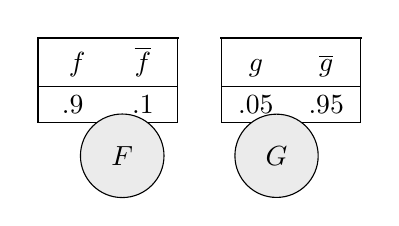
\begin{tikzpicture}[center base, scale=0.7,ampersand replacement=\&]
        % \def\figtabledist{1.4}
        % \def\fignodedist{1.2}
        % \def\figtableheight{0.22}
        \def\figtabledist{0.2}
        \def\fignodedist{1.4}
        \def\figtableheight{0.41} 

        \matrix [table with head, column 1/.style={leftrule}, anchor=south east,
             column 2/.style={rightrule}, row 2/.style={bottomrule}] at (-\figtabledist,\figtableheight) {
            \vphantom{$\overline fg$} $f$ \& \vphantom{$\overline fg$}$\overline f$\\
            .9 \& .1\\
        };
        \matrix [table with head, column 1/.style={leftrule}, anchor=south west,
             column 2/.style={rightrule}, row 2/.style={bottomrule}] at (\figtabledist,\figtableheight) {
             \vphantom{$\overline fg$}$g$ \& \vphantom{$\overline fg$}$\overline g$\\
             .05 \& .95\\
        };
        \node[dpadded, circle, fill=black!08, fill opacity=1] (floomp) at (-\fignodedist,0) {$F$};
        \node[dpadded, circle, fill=black!08, fill opacity=1] (gun) at (\fignodedist,0) {$G$};
    \end{tikzpicture}
    ~~\vrule~~
	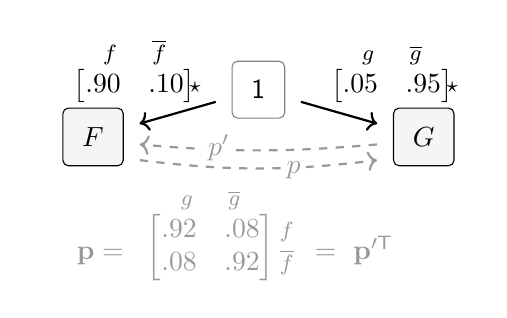
\begin{tikzpicture}[center base]

        \def\fignodedist{2.1}
        \def\fignodeheight{1.1}
        \def\newcptX{-0.3}
        \def\newcptY{-0.1}
                     
		\node[dpadded, fill=white, draw=gray] (true)  at (0,1.7) {$\var 1$};
		\node[dpadded] (floomp) at (-\fignodedist,\fignodeheight) {$F$};
		\node[dpadded] (gun) at (\fignodedist,\fignodeheight) {$G$};			
		
		\draw[arr] (true) -- coordinate(A) (floomp);
		\draw[arr] (true) -- coordinate(B) (gun);

		\node[above left=2.2em of A, anchor=center] {
        %oli14 fix gray.
			% \begin{idxmat}{\!\!\!$\star$\;\;\;}{$f$, $\overline f$}
			\begin{idxmat}[\color{black}\smalltext]{\!\!\!$\star$\;\;\;}{$f$, $\overline f$}
				.90 & .10 \\
			\end{idxmat}
		};
		\node[above right=2.2em of B, anchor=center] {
        %oli14
        % \begin{idxmat}{\!\!\!$\star$}{$g$, $\overline g$}
			\begin{idxmat}[\color{black}\smalltext]{\!\!\!$\star$}{$g$, $\overline g$}
				.05 & .95 \\
			\end{idxmat}
		};
		\definecolor{heldout}{rgb}{0.6, 0.6, .6}	
		\draw[heldout, dashed, arr] (floomp.-30) to[bend right=7] node[pos=0.65, fill=white, inner sep=2pt] (C) {$\smash{p}\vphantom{v}$} (gun.210);
        %oli12: addes reverse arrow, edited the above line with a yshift.
        \draw[heldout, dashed, arr] (gun.190) to[bend left=5] node[pos=0.668, fill=white, inner sep=2pt] {$\smash{p'}\vphantom{v}$} (floomp.-10);
		\node[anchor=center] (newcpd) at (\newcptX,\newcptY) {
			\color{heldout}
			$\mat p =\!\!\!$\begin{idxmat}[\color{heldout}\smalltext]{$f$,$\overline f$}{$g$, $\overline g$}
%joe12
%			  .92 & 0.08 \\ .08 & .92 \\
			  .92 & .08 \\ .08 & .92 \\
          \end{idxmat}$~=~{\mat p'^{\textsf T}}$
		};
        % \node[below=3pt of newcpd] {\color{heldout}$\mat p' = \mat p^{\textsf T}$};
	\end{tikzpicture}
	}
    %oli12 update caption accordingly.
    %oli12: note before editing caption: making it fit on one line is not easy.
	% \caption{An inconsistent PDG, requiring resolution}
%joe11
%        \caption{A BN (left), and respective PDG (right), which can
%oli19: added word "simple" BN
%joe17: why did you add it?  What is a simple BN?
%oli20: Nothing technical. It doesn't look very much like a BN and I
%wanted to assure  
% readers that nothing strange is going on here. I trust your judgement and gether you
% think it's negative, and so am pre-emptively reverting it.
        \caption{A BN (left) and corresponding PDG (right), which can
        include more cpds; $p$ or $p'$ make it inconsistent.} 
    \label{fig:gun-floomp-diagram}
\end{figure}

%oli12
% Now suppose that you later discover that
A traumatic experience a few hours later leaves Grok believing that
%joe11
%``floomp'' is likely (92\%) to be another word for gun.
``floomp'' is likely (probability .92) to be another word for gun.
%oli12: I've removed the directionality by adding arrows in both directions.
%, and come to believe that if floomps are legal (resp., illegal), then
% there's a  chance guns are as well, and vice versa. 
%joe7: r seems like a atrange letter to use, although it's not a big deal
%oli12: I don't care about the letter. let's use p? Also this notation, while 
% you might not like it, is the consensus, especially in the conference we're 
% submitting to. We're already giving them something quite out of the ordinary;
% I don't want  to push it too far.  It's also expedient here as it lets us 
% immediately indicate the direction.
Let $p(G \mid F)$ be the \emph conditional \emph probability \emph
distribution (cpd) that describes 
the belief that if floomps are legal (resp., illegal),
%joe11
%then with 92\% probability, guns are as well, and $p'(F \mid G)$ be
then with probability .92, guns are as well, and $p'(F \mid G)$ be
the reverse. 
%oli12:
% A first reaction might be to
Starting with $p$, Grok's first instinct is to
simply incorporate the conditional information by adding $F$ as a parent of
$G$, and then associating
the cpd
$p$ with $G$. But then what should she do
with the original probability she had for $G$?  Should she just discard it?
It is easy to check that there is no 
%oli12
% probability distribution 
joint distribution
that is consistent with
%oli12 inserted
both
the two original priors on $F$ and $G$ and also 
%oli12: already lots of commas in this sentence. saying "the cpd" too often also gets to be a lot....
%the cpd $\mat r$, so if she
%joe11
%$p$---so if she
$p$.  So if she
is to represent the information with a BN, which always represents a consistent
distribution, she must resolve the inconsistency.  

However,
%oli12: rewrote paragraph.
% it may be better not to sort this out right away. 
% How to resolve it may be clearer 
% if you can get confirmation that guns are indeed floomps, or read the
% laws more carefully.
sorting this out immediately may not be ideal.
For instance, if the inconsistency arises from a conflation between
two definitions 
of ``gun'', a resolution will have destroyed the original cpds. A
better use of computation may be to notice the inconsistency and look
up the actual law. 

By way of contrast, consider the corresponding PDG. In a PDG, the cpds are
attached to edges, rather than nodes of the graph.
%oli12: this discussion is a distraction; it has nothing to do with PDGs over BNs.
 % we don't mention matrices anywhere else anymore, and the matrix representation
 % in the figure is both a common and inutuitive way of describing this
%
% The cpd associated with an
% edge $e$ from $X$ to $Y$ is a matrix $\mat e$, where the element $\mat e_{x,y}$
% at row $x$ and column $y$ is the conditional probability $\Pr(Y \!\!=\!\!y \mid
% X \!\!=\!\! x)$. 
In order to represent unconditional probabilities, we introduce
a \emph{unit variable} $\var 1$ which 
%oli12: no reason to be too verbose here; more important stuff is coming.
% takes on only one possible value, which we denote
takes only one value, denoted
$\star$. 
%oli12: Thus, we have
This leads Grok to 
the PDG depicted in \Cref{fig:gun-floomp-diagram},
where the edges from $\var 1$ to $F$ and $G$ are associated with the
unconditional probabilities of $F$ and $G$, and the 
%oli12
%edge from $F$ to $G$ is associated with the cpd $p$. 
edges between $F$ and $G$ are associated with $p$ and $p'$.



%joe11: if we make everything black, we should get rid of ``black'' in
%the next line.
The original state of knowledge consists of all three nodes and the two
%oli13: the important bit is that they're solid. I'm trying to
%linguistically  exclude the blue/ dashed lines.
% black
solid
edges from $\var 1$. This is like Bayes Net that we considered above,
%joe11
%except we
except that we 
no longer
%oli12! 
explicitly
%joe11
%oli13:  :(  I think "to be" sounds way better. It's shorter, it doesn't expend
% our limited supply of "and", "that" and "are", which tiring quickly. It sounds
% cooloer. That's also definitely how I would say it in person; I
% think the "that 
% ... are" sounds like you're talking to someone you only trust to know simple 
% grammar --- but in fact, "to be" often taught earlier when people learn English
% as a foreign language, so this form is shorter and without an accesibility 
% cost.
% I believe the infinitive also strengthens the statement by not implying a 
% present tense (how is time relevant here?). I'm changing it back. If you have 
% a reason for your aesthetic preference that you think objectively outweighs this
% consideration to a significant degree, you can change it back and I will 
% accept it without argument, but ask you why later.
%
% assume that $F$ and $G$ are independent; we merely record the constraints
%joe12: if you must have ``to be''
%assume $F$ and $G$ to be independent; we merely record the constraints
take  $F$ and $G$ to be independent; we merely record the constraints
imposed by the given probabilities.  
	
The key point is that we can incorporate the new information into our original
representation (the graph in \Cref{fig:gun-floomp-diagram} without the edge from
$F$ to $G$) simply  by adding the edge from $F$ to $G$ and the associated cpd
%joe12: I could accept that the new information is in gray but then
%why are f and \overline{f}, g nad \overline{g}, and * in gray?
%oli14: Fixed. The reason is because I didn't want to draw focus towards the labels.
%$\mat r$. Doing so does not change the meaning of the original edges.  
%oli14:
% $\mat p$ (the new infromation is shown in gray). 
$p$ (the new infromation is shown in blue).
Doing so does not change the meaning of the original edges.   
%oli12: redundant.
% This
% presentation lets us simply include information, and resolve inconsistencies
% later.
Unlike a Bayesian update, the operation is even reversible: all we need
to do recover our original belief state is delete the new edge, 
%oli12: no need for 'effectively'
%effectively
making it possible to mull over and then reject an observation.
%
\end{example}


The ability of PDGs to model inconsistency, as illustrated in
\Cref{ex:guns-and-floomps}, appears to have come at a significant cost. We seem
to have lost a key benefit of BNs: the ease with which they can
capture
(conditional) independencies, which, as Pearl \cite{pearl1989conditional} has
argued forcefully, are omnipresent.
%oli12*: it seems like we should add a sentence fragment here, along
%the lines of "but we will be able to easily recover them".  Also, the
%above is kind of redundant, so I keep looking at it trying to figure
%out how to re-word, but it's so well written that I can't figure out
%what I want to do to it.
%joe11: how about:
%As we shall see, we will be able to recover this information.
%oli13: Most anything we add without cutting down the text before will
%ultimately cost a line. I'm not sure this particular phrase is worth
%it, I've commented it out. 
% Counterproposal:
%joe12: Looks like you didn't finish this here
%joe13*: you still didn't finish this sentence.  I'm cutting it.
%And yet:
%oli15: The intention was to lead directly to the example. It's a
%clever but maybe  
% too-cute transition; it is free (fits on on the line) if you remove a comma. 


% most of the time, we do not make the independence
% assumption in a bn because we know for certain that the
% variables are independent; rather, we just suspect that the
% identified edges are by much more important than the
% others. determining for sure that smoking  and second hand
% smoke are independent, controlling for parents' smoking
% habits, would extremely difficult, and would require
% empiricism to validate. 
	

\begin{example}[emulating a BN]\label{ex:smoking}

We now consider the classic (quantitative) Bayesian network $\cal B$, which has
four binary variables indicating whether a person ($C$) develops cancer, ($S$)
smokes, ($\mathit{SH}$) is exposed to second-hand smoke, and ($\mathit{PS}$) has
parents who smoke, presented graphically in \Cref{subfig:smoking-bn}. We now
walk through what is required to represent $\cal B$ as a PDG, which we call
$\PDGof{{\mathcal B}}$, shown as the solid nodes and edges in
\Cref{subfig:smoking-pdg}. 

\begin{figure*}[ht!]
	\centering
	
	\begin{subfigure}[b]{0.25\textwidth}
		\scalebox{0.9}{
        %oli12: update BN figure to be consistently shaped
		\begin{tikzcd}[center base, column sep=1.0em, row sep=0em, dpad={fill opacity=1,fill=black!08, circle, inner sep=3pt, minimum size=2.3em, draw=gray}, 
			ampersand replacement=\&]
		\& S \ar[dr] \\
		PS \ar[ur]\ar[dr] \&\& C \\
		\& SH \ar[ur]
		\end{tikzcd}}
        \caption{The Bayesian network $\cal B$}
		\label{subfig:smoking-bn}
	\end{subfigure}%
	\hspace{1.5em}\vline\hspace{1.5em}
	\begin{subfigure}[b]{0.57\textwidth}
		\scalebox{0.9}{
		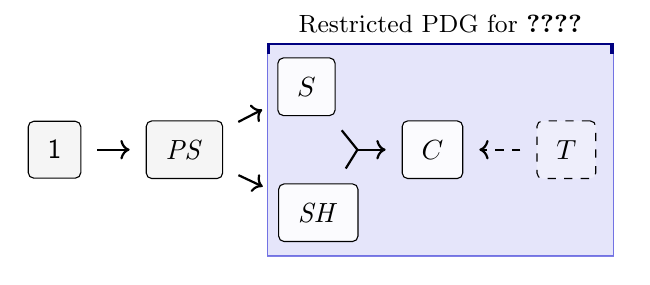
\begin{tikzpicture}[center base]
		\fill[fill opacity=0.1, blue!80!black, draw, draw opacity=0.5] (2.7,1.35) rectangle (7.1, -1.35);
		
		\node[dpadded] (1) at (0,0) {$\var 1$};
		\node[dpadded] (PS) at (1.65,0) {$\mathit{PS}$};
		\node[dpadded, fill=black!.16, fill opacity=0.9] (S) at (3.2, 0.8) {$S$};
		\node[dpadded, fill=black!.16, fill opacity=0.9] (SH) at (3.35, -0.8) {$\mathit{SH}$};
		\node[dpadded, fill=black!.16, fill opacity=0.9] (C) at (4.8,0) {$C$};
		
		\draw[arr] (1) -- (PS);
		\draw[arr] (PS) -- (S);
		\draw[arr] (PS) -- (SH);
		\mergearr{SH}{S}{C}
		
		\node[dpadded, fill=black!.16, fill opacity=0.35, dashed] (T) at (6.5,0) {$T$};
		\draw[arr,dashed] (T) -- (C);	

		\draw[very thick, |-|, color=blue!50!black,text=black] (2.7, 1.35) --coordinate(Q) (7.1,1.35);
        \fill[white] (2.6, 1.36) rectangle (7.2,1.55);
        \useasboundingbox (current bounding box);
        \node[above=0.05em of Q]{\small Restricted PDG for \Cref{ex:grok-ablate,ex:grok-union}};
		
		\end{tikzpicture}}

%oli12: I wasn't really sure what to do with this caption given that it really needs to be 2/3 of a line for the figure to look right.
% \caption{The PDG $\PDGof{{\mathcal B}}$ corresponding to ${\mathcal B}$, and a restriction of it.} 
\caption{The PDG $\PDGof{{\mathcal B}}$, and two alterations of it.} 
		\label{subfig:smoking-pdg}
	\end{subfigure}

    \caption{Graphical models representing conditional relationships in \Cref{ex:smoking,ex:grok-ablate,ex:grok-union}}
	\label{fig:smoking-bn+pdg}
\end{figure*}
		
We start with the nodes corresponding to the variables in $\cal B$, together
with the special node $\sf 1$ from \Cref{ex:guns-and-floomps}; we add an edge
from ${\sf 1}$ to $\mathit{PS}$, to which we associate the unconditional
probability given by the cpd for $\mathit{PS}$ in $\cal B$. We can also re-use
the cpds for $S$ and $\mathit{SH}$, assigning them, respectively, to the edges
$PS \to S$ and $PS \to SH$ in $\PDGof{{\mathcal B}}$.
There are two remaining problems: (1) modeling the remaining table in $\cal B$,
which corresponds to the conditional probability of $C$ given $S$ and $SH$; and
(2) recovering the additional
%oli12 added
conditional
independence assumptions in the BN. 

For (1), we cannot just add the edges $S \to C$ and $SH \to C$ that are present
%joe11: line shaving
%in $\cal B$, because, as we saw in \Cref{ex:guns-and-floomps}, this would mean
in $\cal B$. As we saw in \Cref{ex:guns-and-floomps}, this would mean
supplying two \emph{separate} tables, one indicating the probability of $C$
given $S$, and the other indicating the probability of $C$ given
%joe11: more line shaving
%$\mathit{SH}$. Doing this would lose significant information that is
$\mathit{SH}$.  We would lose significant information that is
present in $\cal B$  about 
how $C$ depends jointly on $S$ and $SH$. To distinguish the joint dependence on
$S$ and $\mathit{SH}$, for now, we draw an edge with two tails---a
\emph{hyperedge}---that completes the diagram in \Cref{subfig:smoking-pdg}. 
%
With regard to (2), there are many distributions consistent with the conditional
marginal probabilities in the cpds, and the independences presumed by $\cal B$
need not hold for them. 
%oli12
% Rather than encoding the extra probabilistic information as cpds,
Rather than trying to distinguish between them with additional constraints,
we develop a a scoring-function semantics for PDGs
%oli12: hmm, the consistency is part of the scoring function. 
%    , and show that, among all distributions consistent with
%    $\PDGof{{\mathcal B}}$,
%joe11: so we're encoding the constraints in the semantics of the
%scoring function, rather than directly in the PDG.  This makes it a
%``soft'' constraint.  We could say that somewhere, but this seems
%like the wrong place.
%joe11: I don't know what ``emphasis on matching (potentially
%arbitrary) cpds'' means 
%which, despite an emphasis on matching (potentially arbitrary) cpds,
which 
is in this case uniquely minimized by the distribution 
%joe8*: I think we need to throw out hints about how we're going to
%use scoring functions.  I view this as critical
%oli12: I think the BN result is strong enough that this is too much hedging.
% for the appropriate scoring function, 
% the unique distribution with a minimum
% score is the one
%
specified by ${\mathcal B}$ (\Cref{thm:bns-are-pdgs}).
This allows us to recover the semantics of Bayesian networks without requiring the independencies that they assume.

%But now suppose that we get information beyond that captured by the
Next suppose that we get information beyond that captured by the original BN.
Specifically, we read a thorough empirical study demonstrating that people who
use tanning beds have a 10\% incidence of cancer, compared with 1\% in the
%joe7: \mat p comes out as a strange symbol in my pdf file.  Why do
%you need to use nonstandard fonts like \mat?
%oli12: It's just \mathbf. I'm surprised it comes out strange. In any case, no
% more \mat for cpds unless they're matrices.
%joe11: this was an old problem, that got fixed by the other changes
%you made.  But I prefer the current notation in an case.
control (call the cpd for this $p$); we would like to add this information to
$\cal B$. The first step is clearly to add a new node labeled $T$, for ``tanning
bed use''.  But simply making $T$ a parent of $C$ (as clearly seems appropriate,
given that the incidence of cancer depends on tanning bed use) requires a
substantial expansion of the cpd; in particular, it requires us to make
assumptions about the interactions between tanning beds and smoking.  
%
The corresponding PDG, $\PDGof{{\mathcal B}}$, on the other hand, has no
trouble: We can simply add the node $T$ with an edge to $C$ that is associated
with $\mat p$.  But note that doing this makes it possible for our knowledge to
be inconsistent. To take a simple example, if the distribution on $C$ given $S$
and $H$ encoded in the original cpd was always deterministically ``has cancer''
for every possible value of $S$ and $H$, but the distribution according to the
new cpd from $T$ was deterministically ``no cancer'', the resulting PDG would be
inconsistent.  
%
\end{example}


We have seen that we can easily add information to PDGs; removing information is
equally painless.   

\begin{example}[restriction]\label{ex:grok-ablate}
%oli12
% After the communist uprising, 
%joe11
%  After the communist party came to power,
  After the Communist party came to power,
  children were raised communally, and so parents' smoking habits no longer had any impact on them. Grok is reading her favorite book on graphical models, and she realizes that while the node $\mathit{PS}$ in \Cref{subfig:smoking-bn} has lost its usefulness, and nodes $S$ and $\mathit{SH}$ no longer ought to have $\mathit{PS}$ as a parent, the other half of the diagram---that is, the node $C$ and its dependence on $S$ and $\mathit{SH}$---should apply as before.
%oli4: this next sentence is less useful, and can be
    %removed; its purpose is to pre-emptively push against
    %a desire to margnialize and get a new BN.  
%joe4: let's remove it
% \begin{edge} 
% 	The rise of the communist party also came with changes in smoking habits, so a new unconditional distribution on $S$ could not be obtained by eliminating the variable $PS$. 
% \end{edge}
Grok has identified two obstacles to modeling deletion of information from a BN
by simply deleting nodes and their associated cpds. First, this restricted model
is technically no longer a BN (which in this case would require unconditional
distributions on $S$ and $\mathit{SH}$), but rather a \emph{conditional} BN
\cite{KF09}, which allows for these nodes to be marked as observations;
observation nodes do not have associated beliefs. Second, even regarded as a
conditional BN, the result of deleting a node may introduce \emph{new}
independence information, incompatible with the original BN. For instance, by
deleting the node $B$ in a chain $A \rightarrow B \rightarrow C$, one concludes
that $A$ and $C$ are independent, a conclusion incompatible with the original BN
containing all three nodes.   
%joe7*: shortened significantly.  I don't think it's
   %worth agonizing this over this.
%oli12: Your shortening is excellent :)
%joe11: :-)
PDGs do not suffer from either problem.  We can easily delete the
nodes labeled 1 and $PS$ in \Cref{subfig:smoking-pdg} to get the
restricted PDG shown in the figure, which captures Grok's updated information.
%oli12: I want to keep some of the material  underneath it for the
%full paper though. 
% I have rewritten a lot of it.
%joe17: I can live with this in the paper
%\begin{vfull}
The resulting PDG has no edges leading to $S$ or $\mathit{SH}$, and hence no
distributions specified on them; no special modeling distinction between
observation nodes and other nodes are required. Because PDGs do not directly
make independence assumptions, the information in this fragment is truly a
subset of the information in the whole PDG. 	
%\end{vfull}
% 
\end{example}

Being able to form a well-behaved local picture and restrict knowledge is
useful, but an even more compelling reason to use PDGs is their ability to
aggregate information. 
	
\begin{example}\label{ex:grok-union}
Grok dreams of becoming Supreme Leader ($\it SL$), and has come up with a plan.
She has noticed that people who use tanning beds have significantly more power
and than those who don't. Unfortunately, her mom has always told her that
%joe11
%tanning beds cause cancer%
tanning beds cause cancer;
%oli12 
%. In particular,
%joe11: I'm not a fan of dashes; there are better punctuation
%oli13: I've noticed. I'm not a purist, except about maximizing the entropy
% of my punctuation :P
%---specifically, that
specifically, that
15\% of people who use tanning beds
get it, compared to the baseline of 2\%.
%oli12: shortening
% Let $q$ be the cpd associated with this belief.
Call this cpd $q$.
Grok thinks people will make fun of her if she uses a tanning bed and
gets cancer, making becoming Supreme Leader impossible. This mental state is
depicted as  a PDG on the left of \Cref{fig:grok-combine}.
%oli12 we haven't left out anything more than we have earlier.
% (where we have left out the cpds, to avoid clutter).


Grok is reading about graphical models because she vaguely remembers that the
variables in \Cref{ex:smoking} match the ones she already knows about. When she
finishes reading the statistics on smoking and the original study on tanning
beds (associated to a cpd $\mat p$ in \Cref{ex:smoking}), but before she has
time to reflect, we can represent her (conflicted) knowledge state as the union
of the two graphs, depicted graphically on the right of \Cref{fig:grok-combine}.  


\begin{figure}
	\colorlet{colororiginal}{blue!50!black}
	\colorlet{colorsmoking}{orange!80!black}
	\tikzset{hybrid/.style={postaction={draw,colorsmoking,dash pattern= on 5pt off 8pt,dash phase=6.5pt,thick},
		draw=colororiginal,dash pattern= on 5pt off 8pt,thick}}
	\centering
	\scalebox{0.8}{
	\begin{tikzpicture}[thick, draw=colororiginal, text=black]
		\node[dpadded] (C) at (0,0) {$C$};
		\node[dpadded] (T) at (2,0){$T$};
		\node[dpadded] (SL) at (1,-1.5){$\it SL$};
		
		\draw[arr] (T) to[bend right] node[above]{$q$} (C);
		\mergearr{C}{T}{SL}
	\end{tikzpicture}
	\hspace{2em}\vline\hspace{2em}
	\begin{tikzpicture}
		\begin{scope}[postaction={draw,colorsmoking,dash pattern= on 3pt off 5pt,dash phase=4pt,thick}]
			
			\node[dpadded,hybrid] (C) at (0,0) {$C$};
			\node[dpadded,hybrid] (T) at (2,0){$T$};
		\end{scope}
		
		\begin{scope}[thick, draw=colororiginal, text=black]
			\node[dpadded] (SL) at (1,-1.5){$\it SL$};
			\draw[arr] (T) to[bend right] node[above]{$q$} (C);
			\mergearr{C}{T}{SL}
		\end{scope}


		\begin{scope}[thick, draw=colorsmoking, text=black]
			\node[dpadded] (S) at (-1.4, 0.8) {$S$};
			\node[dpadded] (SH) at (-1.45, -0.8) {$\mathit{SH}$};
			\draw[arr] (T) to node[fill=white, fill opacity=1,text opacity=1,inner sep=1pt]{$p$} (C);
			\mergearr{S}{SH}{C}
		\end{scope}
	\end{tikzpicture}
	}
	\caption{Grok's prior (left) and combined (right) knowledge.}
	\label{fig:grok-combine}
\end{figure}

The union of the two PDGs, even with overlapping nodes and is still a PDG. This
is not the case in general with a BN. Note that the PDG that Grok used to
represent her two different sources of information (the mother's wisdom and the
study) regarding the distribution of $C$ is a \emph{multigraph}: there are two
edges from $T$ to $C$, with inconsistent information. Had we not not allowed
multigraphs, we would need to choose between the two edges, or represent the
information some other (arguably less natural) way. As we are already allowing
inconsistency, merely recording both is much more in keeping with the way we
have handled other types of uncertainty. 
%		
%TODO: I should not say this yet. This is a related story that I haven't told yet. 
%Moreover, if Grok were to later discover that her mother had been faithfully transmitting the results of an unrelated study, she would be justified in increasing her certainty that a cpd roughly like $\mat p$ and $\mat q$ were correct.
% This suggests a result that is perhaps obvious in retrospect: the mere \emph{possibility} of inconisistency increases the value of consistency. For an agent that is guaranteed to be consistent by design, corroborating evidence has no value. 
\end{example}

Not all inconsistencies are equally egregious. For example, even though the cpds
$p$ and $q$ are different, they are numerically close, so, intuitively, the PDG on the right in
\Cref{fig:grok-combine} is not very inconsistent.
Making this precise 
%oli12:  
% will be
is
the focus of \Cref{sec:scoring-semantics}.


%joe4*: While I don't have an intrinsic problem with this paragraph,
%I'm not sure it belongs in the introduction.  Do we discuss this in
%more detail elsewhere in the paper?   If so, we have to say more
%about it.  As it stands, it seems like a letdown, after quite a
%compelling introduction.  I cut it for now.
%
%oli5: I agree with your assessment that it either needs to be followed
% up by something, or removed---although I'm not sure I agree there needs
% to be more text here. I strongly prefer to follow it up with something;
% I think path composition is one of the most important selling point of PDGs, 
% on par with the ability represent inconsistency, and showcases
% modularity in a useful, compositional way. To reflect this preference,
% I'm uncommenting this, but you're welcome to re-comment it in the next iteration.
%joe5*: commenting out, until you come up with a story for it that
%fits in the paper.  I strongly suspect that it won't make it into a
%NIPS submission, so by commenting it out, we'll be able to better
%judge space.
\commentout{
While a PDG is in some sense merely a set of constraints (the cpds), these constraints themselves have a useful computational meaning. Regarding cpds as stochastic matrices, we can get cpds corresponding to paths by multiplying them; equivalently, thought of as probabilistic functions, we can compose them.
	For instance, in \Cref{ex:grok-union}, if we were to give Grok
        unconditional probabilities in the form of vectors
        $\smash{(\vec s, \vec h, \vec t)}$ over the possible values of
        $\mathit{S, SH}$ and $\mathit T$ respectively, she could
        compute three distinct estimates for $\mathit{SL}$. This is
        perhaps clearest visually, but for clarity, if $\mat S$ is
        the cpd for the orange hyperedge that computes $C$ from
        $\mathit{S, SH}$, and $\mat L$ is the cpd for the
%joe4: the colors may not come across for some people, so you may want
%to use some other way of distinguishing them
%oli5*: Can I rely on colors to distinguish things in general? I've been using it throughout the document. I've seen papers that do this, but I can see why it might be poor taste (e.g., black and white printers). I can add letters to the hyper-edges here.
%        blue hyper edge, which computes $\mathit{SL}$ from $\mathit{C, T}$, and
%        $[\vec a; \vec b]$ is a vertical stacking of the vectors $\vec
    blue hyperedge that computes $\mathit{SL}$ from $\mathit{C, T}$, and we 
%oli5:
% use the notation 
		write
        $[\vec a; \vec b]$ for the matrix with rows $\vec
        a$ and $\vec b$, then 
	\[ \mat L \Big[\mat p \vec t; \vec t\ \Big],
		\qquad \mat L \Big[\mat q \vec t; \vec t\ \Big], \quad\text{and}
		\quad \mat L \Big[\mat S \big[\vec s; \vec h\big], \vec t\ \Big]  \]
	        are all probabilistic estimates of $\mathit{SL}$, which
                can be used in different circumstances: the first two are
        applicable even if given only $\vec t$, and the last requires
        all three values. 
	This property gives PDGs more useful structure than most
        collections of constraints.  
}
%joe5: \end{commentout}
        
These examples give a taste of the power of PDGs.  In the coming sections, we formalize PDGs and relate them to other approaches.		
% \begin{notfocus}
%	\begin{enumerate}[nosep]
%		\item This representation more naturally matches what humans are aware of, encoding small locally consistent models rather than one giant probability distribution
%		\item It is a strictly more general representation--- we can easily convert BNs to these diagrams (section \ref{sec:convert2bn})
%		\item This allows composition of arrows to be defined, and gives meanings to paths (section \ref{sec:composition}).
%		\item Allowing variables to be added and removed makes
%		\item Changing and partially determining arrows is more reasonable.
%		\item We can now represent inconsistency, which will allow us to capture mental states which, and . While we agree with the classical picture in that inconsistency is bad, now we can talk about it
%	\end{enumerate}
% Redundency is important: types in programming languages, more data in ML systems.
% Puts gurads
% Makes it possible to combine knowledge without destroying old knowledge.
% preference updating
	
	
\section{Syntax}\label{sec:formal+syntax}
We now provide formal definitions for PDGs.        
Although it is possible to formalize PDGS with hyperedges directly,
    we opt for a different approach here, in which PDGs have only regular edges,
and hyperedges are captured using a simple construction
that involves adding an extra node.

\vfull{\footnote{In the factor graph literature,
          especially with regard to loopy belief propagation
          \cite{wainwright2007graphical}, it is common to
          call a collection of marginals that are not
          necessarily all compatible with a distribution
          \emph{pseudomarginals}, making a PDG in some sense a
          collection of `conditional' pseudomarginals. This
          gives an alternate, more technically precise
          expansion of PDG as ``Pseudomarginal Dependency Graph''.}}



\begin{defn}[PDG]\label{def:model}
	A \emph{Probabilistic Dependency Graph} is a tuple $\pdgvars[]$ where
	\begin{description}%[nosep]
	\item[$\N$] $\notation{:\Set}$
		is a finite set of nodes, corresponding to variables;
	\item[$\Ed$] $\notation{ \subseteq \N \times \N \times \mathit{Label}}$
		is a set of directed edges, each with a source and target in $\N$, as well as an arbitrary label;
	\item[$\V$] $\notation{\N \to \mathbf{Set}}$
		associates each variable $N \in \N$ with a set $\V(N)$ of values that the variable $N$ can take;
  	\item[$\mat p$] $\notation{\colon \big(\!({A,B,\ell})\colon \! \Ed \big) \to \V(A) \to \Delta\V(B)}$
			% HYPERGRAPH \mat p TYPE: $\colon\!\big(\!({\bf A,B})\colon \! \Ed \big) \to \prod\limits_{A\in \bf A} \!\! \V(A) \to \underline\Delta\left[\prod\limits_{B \in \bf B}\!\!\V(B)\right]$
		associates to each edge $(X,Y,\ell) \in \Ed$ a distribution $\bp(x)$ on $Y$ for each $x \in \V(X)$; 
% %joe8*: I thought of adding \alpha, then decided it was a bad idea; see below
%oli20: added temporarily so you can see what I'm envisioning
	
	\item[\contentio{$\alpha$}] \contentious{$\notation{}$
	 	associates a non-negative real number $\alpha_L$ 
 		to each link $L$,
%joe18: it would be fine if we could ever agree on what it meant.
%indicating an agent's confidence in the functional (and we have tried
%many times in the past ...)
%       	 	dependence suggested by $L$ } 
	 	dependence suggested by $L$;} 
	\item[$\beta$] $\notation{:\Ed \to \mathbb R^+}$
		associates a positive real number $\beta_L$ to each edge $L$, indicating an agent's subjective confidence in the reliability of cpd $\bp$. 
%joe8*: can't the number be 0?  Also, is higher intended to be better;
%if so, we should say that.  But that means that we can't indicate
%complete certainty.  I would prefer to use a number in [0,1].  Is
%there a reason we shouldn't take \beta \in [0,1]
%oli10: 
% I think \beta=0 should be allowed, but if there is a \beta=0, we
% will use uniqueness guarantees. Also, this would effectively just
% contribute to the qualitative picture of the PDG, which is currently
%joe9: I don't understand what you said above.  What do ``uniqueness
%guarantees'' have to do with anything?
%joe10: I puzzled over this until I realized that you probably meant
%``lose [not use] uniquenes guarantees'' above and ``if \beta can be 0
%oli12: Oops, I don't know how I made both typos. You're correct.
%[not positive] below.  If that's not right, I'm badly confused.
\end{description}
\end{defn}

If $\dg M$ is a PDG, we reserve the names 
$\pdgvars[^{\dg M}]$
% $\N^{\dg M}$, $\Ed^{\dg M}$, and so forth,
for the components of $\dg M$, so that we may reference one without naming them
all explicitly. We write $\V(S)$ for the set of possible joint settings of a set
$S$ of variables; in particular, we write $\V(\dg M) = \prod_{N \in \N^\dg M}
\V^\dg M(N)$ for all settings of the variables $(\N^\dg M, \V^\dg M)$. 	

While the definition above is sufficient to represent the class of all legal
PDGs, we often use two additional bits of syntax to represent common
constraints:  
    
\begin{itemize}
    \item A special variable $\sf 1$ whose range consists of only element, which
    we denote $\star$. It is used to represent unconditional distributions, as
    in \Cref{ex:guns-and-floomps,ex:smoking}.  
%joe17* I would cut this.  As I said above, it breaks the flow and is
%unnecesary; the examles sffice
%oli20: oops, did not intend to reinsert this. 
\vleftovers{
		\begin{example}\label{ex:worldsonly}
			A probability distribution $p$ over a measurable set $W$ of possible worlds is represented as 
			\begin{center}
				\scalebox{0.8}{
				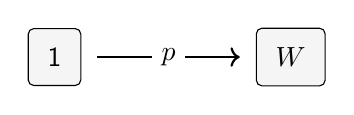
\begin{tikzpicture}
					\node[dpadded] (1) at (0,0) {$\sf 1$};
					\node[dpadded] (W) at (3,0) {$W$};

					\draw[arr] (1) to node[fill=white]{$p$} (W);
				\end{tikzpicture}}
			\end{center}
		\end{example}
}%joe17 \end{vleftovers}

		\item Double-headed arrows, $A \tto
                  B$, which visually indicate the degenerate special
                  case of a cpd that assigns probability 1 to $f(a)$
                  for each $a \in A$ (corresponding to a deterministic
                  function $f : A \to B$). 
\end{itemize}


\begin{constr}\label{constr:hyperedge-reducton}
We can now explain how we capture   the multi-tailed edges that 
were used in 
\Crefrange{ex:smoking}{ex:grok-union}. 
That notation can be viewed as shorthand for the graph that results by adding a new node at the junction representing the joint value of the nodes at the tails, with projections going back.  For instance,
% the diagram of the PDG in the shaded box of \Cref{subfig:smoking-pdg}
the diagram displaying Grok's prior knowledge in \Cref{ex:grok-union}, on the left of \Cref{fig:grok-combine}
%joe7: moved up from below, to save a line
%is really shorthand for the following PDG:
is really shorthand for the following PDG, where
where we insert a node labeled $C \times T$ at the junction:
		\begin{center}
		\scalebox{0.8}{
		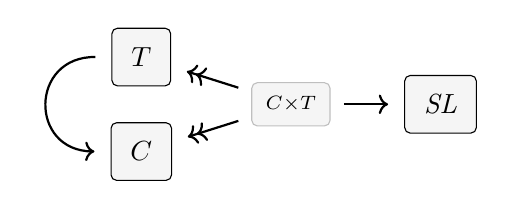
\begin{tikzpicture}
			\node[dpadded] (SL) at (-1.0,0) {$\mathit{SL}$};
			
			\node[dpadded,light pad] (CT) at (-2.9, 0){$\scriptstyle C \times T$};
			\node[dpadded] (C) at (-4.8, -0.6) {$C$};
			\node[dpadded] (T) at (-4.8, 0.6) {$T$};
			
	%				\node[dpadded, dashed,color=violet] (X) at (6.5,0) {$X$};
	%				\draw[arr, color=violet] (X) -- (S);
	%				\draw[arr, color=violet] (X) -- (C);
	%				\draw[arr, dashed, color=violet] (X) -- (SC);
			
			\draw[arr, ->>] (CT) -- (C);
			\draw[arr, ->>] (CT) -- (T);
			\draw[arr] (CT) -- (SL);
			\draw[arr] (T) to [bend right=90, looseness=2] (C);
	\end{tikzpicture}}
	%%%%%%%%%%%%%%%%%  smoking fragment: %%%%%%%%%%%%%%%%%%%%%%
% 		\scalebox{0.8}{
% 			\begin{tikzpicture}
% 				\node[dpadded] (C) at (-1.0,0) {$C$};
% 				\node[dpadded] (T) at (0.5,0) {$T$};
% 
% 				\node[dpadded,light pad] (SSH) at (-2.9, 0){$\scriptsize \mathit{SH} \times S$};
% 				\node[dpadded] (S) at (-4.8, 0.6) {$S$};
% 				\node[dpadded] (SH) at (-5.0, -0.6) {$\mathit{SH}$};
% 
% %				\node[dpadded, dashed,color=violet] (X) at (6.5,0) {$X$};
% %				\draw[arr, color=violet] (X) -- (S);
% %				\draw[arr, color=violet] (X) -- (C);
% %				\draw[arr, dashed, color=violet] (X) -- (SC);
% 
% 				\draw[arr, ->>] (SSH) -- (S);
% 				\draw[arr, ->>] (SSH) -- (SH);
% 				\draw[arr] (SSH) -- (C);
% 				\draw[arr] (T) -- (C);
% 		\end{tikzpicture}}
	\end{center}

% That is, we inserted a node labeled $SH \times S$ at the junction.  As
% the notation suggests, $\V( \mathit{SH} \times S) = \V(\mathit{SH}) \times \V(S)$.
% The cpd for $(h,s) \in \V(\mathit{SH} \times S)$  associated with 
% the edge from $\mathit{SH} \times S$ to $\mathit{SH}$ gives probability 1 to $h$;
% similarly, the cpd for $(s,c)$  associated with 
% the edge from $ C \times C$ to $S$ gives probability 1 to $s$.
%joe7
%        That is, we inserted a node labeled $C \times T$ at the junction.
As the notation suggests, $\V( C \times T) = \V(C) \times \V(T)$.
%joe2: this is not the time to start talking about matri\mathit{SL}es
%Thus, $\V(S \times \mathit{SL}) = \V(S) \times \V(\mathit{SL})$; the matrix asso\mathit{SL}iated with
For any joint setting $(c,t) \in \V(C \times T)$ of both variables, the cpd for
the edge from $C \times T$ to $C$ gives probability 1 to $c$;
similarly, the cpd for the edge from $ C \times T$ to $T$ gives probability 1 to $t$.
\end{constr}

%oli11: Quickly hint about why this works syntactically, so we can
%better summarize this contribution
%joe10*: NO!!!  This ha nothing to do with our story, It's a complete
%distraction.  I don't see the connection between a failure of
%consistency and a failure to commute (and I have a Ph.D. in
%mathematics and no exactly what the words mean).  I *strongly* object
%to including this.  If you have some interesting theorems to prove,
%you can write another paper on it.  You can also talk about it in
%your thesis if you really care.  But not in the paper!  Even if we
%could afford the space (which we can't) I would strongly object.
%oli12*: Are you serious that you don't see the connection?? We should
%talk about this.
%joe11: Yes, I'm serious.  We can discuss it after the deadline.
% I really do think it's a massive oversight not to at least mention
% this. I can see a world where mentioning this is the most important
% thing we do in the paper. I also think you hugely underestimate how
% many people care about commutative diagrams, what this buys you, and
% the implications for mathematical reasonsing.
%joe11: There are certainly people who care about this material.  They
%are an extremely small subset of the NeurIPS community.  We're
%submitting this paper to NeurIPS.  You're more than welcome to write
%a paper about this for a conference where there are substantially more pepole
%who care about commutative diagrms.
%joe17: We *definitely* should not be talking about commuatative
%diagrams at this point in the paper (frankly, I don't think we should
%talk about them at all in the paper
%oli20: agreed, did not intend for this to resurface.
\vleftovers{
    We have stressed that edges are interpreted differently in PDGs than
    in Bayesian Networks. Readers should be aware that this approach is
    closely related to the notion of a \emph{commutative diagram}, a
    common representation in pure mathematics. For those familiar with
    them, the potential failure of a PDG to be consistent is analogous to
    the possibility that a diagram could fail to commute. 
}

%joe4*: cut this paragraph.  It's a distraction.  Moreover, BN's don't
%need this ``trick'', because of the way they interpret the edges.  
\section{Semantics}\label{sec:semantics}
%oli12: I dislike the sentence below. Primarily, it seems like
%cheating to come up 
% with totally different semantics depending on what you want to capture, and 
% we're really not doing that --- our three semantics are intimately
% related, and 
% can all be represented naturally in terms of the scoring function. 
%   There is more than one way of giving semantics to a PDG.  
%oli12: I think something along these lines has the additional benefit of 
% quickly speaking to why we're doing this (people write down cpds all the time). 
Although the meaning of an individual cpd is clear, we have not yet given 
%joe11: you seem to like using ``local'' and ``global'' a lot.
%Although I understand what you intend here, I'm still uncomfortable
%about the usage, because it suggests that there's a local semantics.
%oli13: There is a local semantics: the cpd itself already is a local
%probabilistic object. It is already useful on its own. You can even compose
%them, etc,... But there's ambiguity in stitching them together. In some sense
%this is the problem we address.
%joe12: but we have never talked about local semanatics or local
%probabilistic objects.  This is not the time to start!
%oli14: Anecdotally, this is the point that convinced me that semantics was 
% actually worthwhile. Many people just use cpds by themselves; I'd guess many
% ML people will be wondering why we need anything else if we already have
% the cpds that we need. Can't you just do math with those? In any
% case, "global" 
% is good enough for me.
%joe11: I left it in with the quotation marks.
%oli13: The "local" and "global" is going to also help make sure these terms
% don't come out of the blue later in the paper.
%joe12: but they come out of the blue here.  Do we really need them?
%Are they adding something useful to the discussion?  (As you can
%guess, I don't think that they do.)
%oli14: I think they are. I think this "global" here is already worth it
% even if we don't follow up. I have plenty of following up to do, but
% probably anything substantive won't make it. I have just a few
% characters on the final page. 
%PDGs any global semantics. We discuss three related approaches. The first
%joe14
%PDGs a ``global'' semantics. We discuss three related approaches. The
PDGs a ``global'' semantics. We discuss three related approaches to doing so.
The first is the simplest: we associate with a PDG the set of distributions that
are consistent with it. This set will be empty if the PDG is inconsistent.
%
The second approach associates a PDG with a scoring function, indicating the fit
of an arbitrary distribution $\mu$, and can be thought of as a \emph{weighted}
set of distributions \cite{HL12}. This approach allows us to distinguish
inconsistent PDGs, while the first approach does not. The third approach chooses
the distributions with the best score, typically associating with a PDG a unique
distribution.

%joe18*: Oliver, can you reinstate subsection numbers?
\subsection{PDGs As Sets Of Distributions}\label{sec:set-of-distribution-semantics} 
We have been thinking of a PDG as a collection of constraints on distributions,
specified by matching cpds. From this perspective, it is natural to consider the
set of all distributions that are consistent with the constraints.

\begin{defn} \label{def:set-semantics} 
If $\dg M\sheq\pdgvars[]$ is a PDG, let $\SD{\dg M}$ be the \emph{s}et of
\emph{d}istributions over the variables in $\dg M$ 
%oli12: "the conditional probabilities" is ambiguous, I thought it was reffering
%to p. For a joint distribution p, it's the conditional _marginal_ on the
%appropriate variables that's of interest.
% for which the conditional probabilities are exactly 
%joe11
%whose conditional marginals on are exactly those given by $\mat p$.
whose conditional marginals are exactly those given by $\mat p$.
%oli20: edges have labels (but no need to draw attention to them)
% That is, $\mu \in \SD{\dg M}$ iff, for all edges $L = (X,Y) \in \Ed$,  $x \in
That is, $\mu \in \SD{\dg M}$ iff, for all edges $L \in \Ed$ from $X$
to $Y$,  $x \in 
\V(X)$,  and $y \in \V(Y)$, we have that $\mu(Y = y \mid X\sheq x) = \bp(x)$.
\notation{Formally,		
    \[ \SD[\Big]{\dg M} = \!\left\{\mu \!\in\! \Delta \V_\none (\dg M) \middle|\!
        \begin{array}{l}
        \mu(B\!\! =\!\! b \mid A\!\!=\!\! a) \geq \bp(b \mid a) \\[0.1em]
        ~\text{$\forall (A, B,\ell) \!\in\! \Ed$, $a \!\in\!\V(A)$, $b \!\in\! \V(B)$} 
   		\end{array}\!\!\! \right\}\]
    }
% $\dg M$ is \emph{consistent} if $\SD{\dg M} \ne \emptyset$, and inconsistent otherwise.
% $\dg M$ is \emph{inconsistent} if $\SD{\dg M} = \emptyset$, and consistent otherwise.
$\dg M$ is \emph{inconsistent} if $\SD{\dg M} = \emptyset$, and \emph{consistent} otherwise.
\end{defn}

%joe17*: This breaks teh flow here.  If it were go anywhere, it should
%be in the appendix
%oli20: oops, I don't want it in the AAAI submission either.
\vleftovers{
	It turns out that this semantics only results in convex sets. This may provide useful intuition, and we will prove a stronger version of this statement that corresponds to our second semantics.
	\begin{lemma}[restate=thmsetconvex] 
		\label{prop:convex}
		$\SD{\dg M}$ is convex, for any PDG $\dg M$.
	\end{lemma}

	Note that being inconsistent is not the same things as \emph{over-constrained}: 	
	\begin{defn}
		$\dg M = \pdgvars[]$ is over-constrained if there exists
		  \emph{some $\mat p'$} assigning cpds to the same edges as
		  $\mat p$, such that $(\N, \Ed, \V, \mat p')$ is inconsistent
		  \notation{(i.e., $\SD{\N^\dg M, \Ed^\dg M, \V^\dg M, \mat p}
			= \emptyset$)}, and under-constrained if there are
		  multiple distributions in $(\N, \Ed, \V, \mat p')$ for
		  \emph{every such $\mat p'$}, making this a property of the
		  qualitative PDG $(\N, \Ed, \V)$.  
	\end{defn}

	We know that an under-constrained PDG is consistent without even looking at the tables. However if a we know that an \emph{over-constrained} PDG is actually consistent (when it could have easily contradicted itself), the information provides corroborating evidence, and one can take this as support in favor of the beliefs. 
}

\subsection{PDGs As Distribution Scoring Functions} \label{sec:scoring-semantics}   

We now generalize the previous semantics by viewing a PDG $\dg M$ as a
\emph{scoring function} that, given an arbitrary distribution $\mu$ on $\V(\dg
M)$, returns a real-valued score indicating how well $\mu$ fits $\dg M$.
Distributions with the lowest (best) scores are those that most closely match
the cpds in $\dg M$, and contain the fewest unspecified correlations.
% We now make this precise.

We start with the first component of the score, which assigns higher scores to
distributions that require a larger perturbation in order to be consistent with
$\dg M$.  
%
We measure the magnitude of this perturbation with relative entropy. In
particular, for each edge $L = (X,Y, \ell)$, and each $x \in \V(X)$, we measure
the relative entropy from $\bp(x)$ to $\mu(Y \!= \cdot\mid X=x)$, take the
expectation over $\mu_X$ (that is, the marginal of $\mu$ on $X$). We then sum
over all the edges $L$ in the PDG, weighted by their reliability.


\begin{defn}\label{def:inc}
%oli19: swapping \mu and {\dg M} to shift foucs.
	% The \emph{incompatibility} of a PDG $\dg M = \pdgvars[]$ with
	% a joint distribution $\mu$, denoted $\Inc_{\dg M}(\mu)$, is  
    For a PDG $\dg M$, the \emph{incompatibility} of a
    a joint distribution $\mu$ over $\V(\dg M)$, is given by
    \[
%oli19: removed \pdgvars above, putting ^{\dg M} subscripts here instead.
	\Inc_{\dg M }( \mu) := 
		\!\!\!\!\!\sum_{\ed LXY \in \Ed^{\dg M}} \!\!\beta_L^{\dg M} \E_{x \sim \mu_{_X}}
%oli19: no \cdot to make equation fit on one line. The fact that it is a 
% distribution should be clear because both that this is standard notation, and
% because of the definition of KL divergence that follows. 
% \left[\kldiv[\Big]{ \mu(Y\!= \cdot\mid X \sheq x) }{\bp(x) } \right] ,
\left[\kldiv[\Big]{ \mu(Y \mid X \sheq x) }{\bp^{\dg M}(x) } \right] ,
	\]
	where $\kldiv{\mu}{\nu} = \sum_{w \in \text{Supp($\mu$)}} \mu(w) \log\frac{\mu(w)}{\nu(w)}$ is the 
	relative entropy from $\nu$ to $\mu$.
%joe17: If we use this at all, it should be defined where it's used,
%not here
%oli20: oops, fixed.
\vfull{
	The \emph{inconsistency of PDG $\dg M = \pdgvars[]$}, denoted $\Inc(\dg M)$, is the minimum possible incompatibility of $\dg M$ with any distribution $\mu$,  
	\[ \Inc(\dg M) = \inf_{ \mu \in \Delta [W_{\cal V}]} \Inc_{\dg M}(\mu) . \]
}
\end{defn}

%joe17*: cutting this.  This might be useful if we used it somewhere
%(in which case it should probably go where it's used, not here), but we don't.
%oli20: agreed, updating comment.
\vfull{
    The idea behind this definition of inconsistency is that we want to choose a
    distribution $\mu$ that minimizes the total number of bits required to
    encode all of the relevant conditional marginals. More precisely, fix a
    distribution $\mu$. For each edge $L = (X, Y, \ell) \in \Ed$ and $x \in
    \V(X)$, we are given a code for $Y$ optimized for the distribution $\bp(x)$,
    and asked to transmit data from $\mu(Y\mid x)$; we incur a cost for each bit
    required beyond what we would have used had we used a code optimized for the
    actual distribution $\mu(Y\mid X=x)$. To obtain the cost for $L$, we take a
    weighted average of these costs, where the weight for the value $x$ is the
    probability $\mu_X(x)$. We do this for every edge $L \in \Ed$, summing the
    cost.

    For even more intuition, imagine two agents ($A$ and $B$) with identical
    beliefs described by a PDG $\dg M$ about a set of variables that are in fact
    distributed according to $\mu$. For each edge $L = (X,Y, \ell) \in \Ed^\dg
    M$, values $x,y \in \V(X)$ are chosen according to $\mu_{_{XY}}$ and $x$ is
    given to both agents. 

    At this point, the agents, having the same conditional beliefs, and the same
    information about $Y$, agree on the optimal encoding of the possible values
    of $Y$ as sequences of bits, so that if $y$ were drawn from $\bp(x)$, the
    fewest number of bits would be needed to communicate it in expectation. The
    value of $y$---which is distributed not according to $\bp(x)$, but $\mu(Y
    \mid X=x)$---is now given to agent A. The agents pay a cost equal the number
    of bits needed to encode $y$ according to the agreed-upon optimal code, but
    reimbursed the (smaller) cost that would have been paid, had the agents
    beliefs lined up with the true distribution $\mu$.

    Repeating for each edge and summing the expectations of these costs, we can view
    $\Inc_{\dg M}(\mu)$ as the total number of \emph{additional} expected
    bits required to communicate $y$ with a code optimized for
    $\bp$ instead of the true conditional distribution   $\mu(Y \mid X=x)$. 

    If $\dg M$ is inconsistent, then there will be a cost no matter what
    distribution $\mu$ is the true distribution. Conversely, if $\dg M$ is
    consistent, then any distribution $\mu \in \SD{\dg M}$ will have $\Inc_{\dg
    M}( \mu) = 0$.  

	\begin{example}[continues=ex:worldsonly]
	    Recall our simplest example, which directly encodes an entire distribution $p$
	    over the set $W$. In this case, there is only one edge, the expectation is over
	    a single element, and the marginal on $W$ is the entire distribution. Therefore,
	    $\Inc(\dg M; \mu) = \kldiv{\mu}{\mu}$, so the inconsistency is just the
	    information $\mu$ and $p$, so is minimized uniquely when $\mu$ is $p$
	\end{example}
}
	
$\SD{\dg M}$ and $\Inc_{\dg M}$ distinguish only
between distributions based on their compatibility with
$\dg M$, but even among distributions that match the
marginals, some more closely match the qualitative structure
of the graph than others.  
\commentout{
    Suppose an agent has a PDG $\dg M$ in mind, and imagines that all sample
    variation in a joint distribution $\mu$ over $\V(\dg M)$ arises as a result
    %joe9*: In the next line, did you mean ``some'' or ``each''? See my
    %next joe9*
    %oli11: Both words are ambiguous because of the sentence structure,
    %but I meant to say that we imagine the distribution is generated by
    %rolling the dice in each link. What we do is clear from the
    %formula. I think this is why I prefer putting the formula before the
    %explanation --- people read the explanation already knowing what
    %you're going to do, and then learn why you do it.
    %joe10: there are reasons to put intuition before the formula, and
    %reasons to put after.  I generally prefer giving a high-level
    %intuition first, and then following up with more intuition after the
    %formula if it's would help                
    of sampling the value of a target variable $Y$ of some edge $\ed LXY$, given the
    value of $X$. If this is the case, one would expect the total amount of
    information required to communicate a sample of $\mu$ to be the same as the
    total amount of the information required to separately encode, for
    each edge $\ed LXY$, the randomness of $Y$ given $X$.

    For an arbitrary PDG and $\mu$, these two quantities will differ; if the amount
    of uncertainty in the distribution is lower than one would expect from the
    edges, the distribution has an \emph{information deficiency}, indicating that there
    are additional correlations between variables that are not captured by the
    graph. The higher the information deficiency, the worse the qualitative fit between
    the PDG and $\mu$.
    %joe9*: Now you lost me.  What is ``surplus uncertainty''? This needs
    %tob e given *much* more intuition.
    On the other hand, if a distribution has surplus uncertainty, using it confers a
    benefit. For instance, a PDG containing only the variable $X$
    %joe9* I strenously object to the use of ``safest'' in the way you've
    %used it below.  What is safe depends on utilities, which we haven't
    %mentioned. 
    %oli11: I think this is false. While to express "safe" in general, you
    %would need a utility function, I claim that there is not *any*
    %utility function that, over the joint space of random variables here,
    %would change this calculus at all (except to make it so that you
                    %don't care).
    %joe11: I dsagree; you're too wedded to maxent.  But this is not the
    %time to have this battle                
    % there's 
    %oli13: (This part is still commented out.)
    %joe12: good; let's keep it that way :-)
    and no
    edges encodes awareness about $X$ but no beliefs about it. Given that $X$
    could be distributed in any way (even chosen adversarially), it is safest to act
    as though you believed $X$ to be uniform.  
    %oli11: irrelevant because commented out anyway, but I think what I
    %wrote is more coherent than the below.  and no edges leading to $X$
    %means that the agent is  aware of $X$, but has no  information
    %regarding the probability of various values of $X$ but no 
    We measure the surplus/deficit with a quantity we call
    the \emph{information fit} ($\IDef$) (between ${\dg M}$ and $\mu$):
}
%oli11: end comment. The summary at the end of our meeting was,
%" Given a distribution, compare the cost of specifying \mu directly
%to the cost of specifying the information on the edges for \mu.". You
%also said not to say anything about samples, but it's information
%required to specify a sample of the distribution, given the
%distribution. I'll try a slightly different appraoch, but I don't
%have a good idea about what's going to stick. 
%Let $G$ be a (multi-)graph whose nodes correspond to random variables. 
%joe10
%Each edge $\ed LXY$ of a PDG $\dg M$ represents a qualitative claim
We think of each edge $\ed LXY$ of a PDG $\dg M$ as representing a
qualitative claim that the value of $Y$ can be (noisily) computed from
$X$ alone.  
%
%joe10*: I'm not happy about his, because ``amount of variation'' is
%not well defined. Whateever intuitions you're suggesting here is (in
%my opinion) too closely tied to entroyp.  As a technical matter, I
%think you want to talk about \mu matching \dg M.  Also, in fact, it
%does not match the definition, since it doesn't say what to do with
%parallel edges
%oli13: We already talk about matching in the sentence above.
%oli13: ALso the parallel edges is the reverse of what I'm talking about here.
%How do I people from getting this mixed up? If you think about it carefully.
%With parallel edges (b) > (a) and as we've said, there are additional
%correlations that allow for a more  compact representation. That's the case
%that parallel edges push towards ( and of course the total score is just in
%net). We still need to give intuition for the other case though; here we need
%to say something about the case when (for instance) there are no edges at all.
%joe12: I didn't understand what you wrote above
%   A joint distribution that qualitatively matches $\mu$ will intuitively
%   have as much variation as possible, except where we have claimed that
%   one variable depends on another.
%oli13*: Ok, but we need to impart slightly more detailed intuition instead of
% saying this. I know you don't like entroyp, but given that our formua uses
% entropy (Sorry), and we need to  say something of intermediate formality here
% that gives the right intuition --- we need to say something about variation, 
% or something else that's equivalent with different words. That's the 
% concept we need to communicate here. It doesn't matter if it's undefined, we
% are about to define it. You do a good job explaining it. We'll explain it 
% eve more carefully in the appendix. I promise you nobody at Neurips will care.
% People take so much information theory (and whatever else) for granted; for 
% the full paper, I think we can say enough to make you happy, because I belive
% it really is well-motivated.
%joe12: sometimes less is more.  If you can impart useful intuition.
%oli14: THe reason I keep changing your words in this particular
%section is not 
% because I don't like the way they sound, but because I think they either say
% almost nothing, or they are slightly wrong / misleading. Considering the 
% (perhaps regretably) standard % culture of talking in a cavalier way about
% information, I think I have a bit better sense of how to impart useful
% intuition about entropy.
%I'd *strongly* prefer to say something well in the appendix and nothing
%here rather than saying something not-so-good or unclear here.   
%that's good.  If what you impart is not so useful, then not so good.
%oli13: The current sentence does not serve the correct purpose (and its purpose has
% alredy been fulfilled by the first sentence in the paragraph).
% Thus, given ${\dg M}$, for each measure $\mu$, we consider how well
% the structure of ${\dg M}$ matches that of $\mu$.
%oli14*: I actually really like this sentence, save for the word "anything" 
% (which may be replacable but I could not do easily without either
% being more vague or 
% technical than is your standard preference)
% Think about it carefully before you change it. 
    % The best description of an outcome drawn from a joint distribution that 
%oli16: deleting entire sentence, starting over below.
%joe13
%qualitatively matches $G$, should intuitively both be efficiently
    % qualitatively matches $G$ should intuitively both be efficiently
%oli16
    % described by $G$
    % wherever $G$ has an edge,
%oli16: I'm not super happy with the two lines above either.  line below added
% and then removed.
% described by the conditional outcomes of each edge of $G$,
%joe13
%while also encoding uncertainty about
%oli15: it's not just dependence--- it's technically not accurate
%because there's also the univariate case! 
% while also not having dependences between variables where there is
% no edge in $G$.
%joe14*: Sorry; I do not understand ``maximal information'' in the next
%line.   %This has to be rewritten.  My preference would be for
%reinstating what I wrote.   I don't understand the issue with the
%univariate case, and evenif there is an issue with the univariate
%case, it doesn't prevent what I wrote from being good intuition.
%oli16: the problem is that   
% while also being requiring maximal information to encode relationships
% not in $G$ [[REWRITE]]. 
%oli16: It's so very difficult to write this sentence without making
%it technical, talking 
% about information, or lying....
%oli16: What I had before:
    % The best description of an outcomedrawn from a joint
    % distribution that qualitatively matches $G$ should intuitively
    % both be efficiently described by $G$ wherever $G$ has an edge,
    % while also requiring maximal information to encode relationships
    % not in $G$. 
%oli16: I did a bunch of rewrites, and kept the last 4 in the comments below.
%oli16:rewrite 1:
    % A distribution $\mu$  qualitatively matches $G$ well if it is
    % efficient to describe the outcomes along the edges of $G$, but
    % hard to describe features of $\mu$ that are not encoded by the
    % edges of $\mu$.  
%oli16:rewrite 2:
% pros: no lies, short, should be reasonable intuition. 
% cons: "respect" and "relationships" are vague.
%joe15: this didn't help at all.  I don't understand what it means to
%be ``inefficient to describe''.  It's OK to lie a little when giving
%intuition.  We said above than an think of edge from X to Y as
%''representing a qualitative claim that the value of $Y$ can be
%(noisily) computed from $X$ alone.'' If you want to say something about
%non-edges, it should be that there is no edge from X to Y if we can't
%compute X from Y alone.  If you think that's not quite right, then
%it's better to say nothing than to say something which is likely to
%confuse the reader, especially given how we've described the meaning
%of an edge.
%oli17: I don't think that saying that helps bridge the gap between this idea
%and the next one. I am willing to settle with the document in its current
%state. However, if you read these two paragraphs again closely, you will see
%a rather large chasm between the "qualitatively described just by X" bit, and
%the "information requird to draw a sample" bit. We do not explain why they are
%related. We might modify the first part, but we cannot delete it because we
%need to talk about the qualitative nature of a link; I think that changing the
%secong part significantly is an even bigger mistake, as this is the best
%intuition we give for the equation.
%
%$G$ should be inefficient to describe in every respect except those
%relationships that are encoded by the edges of $G$.  
%oli16:rewrite 3:
% pros: technically accurate
% cons: not the clearest why this is desirable. 
    % We judge a distribution $\mu$ to qualitatively fit $G$ better
    % when the features of an outcome $\mat w \sim \mu$ that follow
    % from the conditional outcomes of $G$ are easy to describe (given
    % $\mu$), and worse when any other features (i.e., those not
    % described by $G$) of $\mat w$ are easy to describe (given
    % $\mu$). 
%oli16:rewrite 4:
% pros: still accurate, more explicit about why it works
% cons: not very eloquent, and might require some of the figures to
% really see why this is the same as the formalism. 
    % Intuitively, a distribution is most likely to have been
    % generated by the edges of $G$ if the information required to
    % specify a the target variables of $G$ directly is no more than
    % the information required to sample separately along the edges of
    % $G$. If $\mu$ makes it easy to describe other aspects of a
    % sample, that $G$ does not articulate, this counts against the
    % match, because we imagine that $G$ would have included these
    % edges if they were easy to communicate qualitatively. 
%oli13: This "anything" is intentionally vague. We cannot clarify this with 
% just the variables it says nothing about, because cycles are possible. 
%joe12*: NO!  I don't know what it means, and I won't accept vagueness
%here.  It's better to cut it!  I need to go now; I'll come back to
%this around 2.
%oli14: Ok, I'll try something slightly less vague.
% anything
%joe13: cut
%\todo{anything}
%that is not described by $G$.
%joe10
%To formalize this, we require only the underlying multigraph $G :=
To formalize this, we require only the underlying multigraph $G^{\dg M} :=
(\N^{\dg M}, \Ed^{\dg M})$ of $\dg M$. 
%joe10: I'm not ure where there ``are known'' is coming from
%oli12: I don't think this is strictly necessary, but it could be useful
% clarification. It seems you (and sometimes I) sometimes get
% mixed up about what exactly this information means.
% The point is that it's the information needed to specify
% the outcome if you already know it is drawn from \mu. 
%joe11: the sentence with ``are known'' doesn't even parse.  Let's
%just leave it.
%oli13: Oops, this parses though (I don't think the "we thus" buys us anything except fluff):
%joe13: whether or not \mu is known is irrelevant!  Why empahsize it
%For a fixed $G$ and known $\mu$, contrast the amount
%oli15: very false. \mu has to be common knowledge! I won't change
%joe14: knowledge has nothing to do with anything here!  There are no
%agents in the picture in this definition.
%oli16: We're now heavily leaning on the term "description", which I argue
% is effectively knowledge. As a technical matter, the way we
% calculate the length of this  
% description assumes that the distribution \mu is known to both the
% sender and reiever of the description.
%joe15: I don't see why.  A calculation is a mathematical expression.
%At best you can say that they way you *use* the result of the calculation is
%meaningful only if something is common knowledge,  but that would
%depend on the usage.   The calculation itself does not depend on
%knowledge. There is no sender and receiver anywhere in our formalism.
%oli17: Ok no more agentive terminology. For the  "description" metaphor to make
%sense, it's necessary that the description gets to exploit the distribution.
%Therefore both the construction of the description, and the interpretation of
%the description, must depend on \mu. Are we now on the same page?
%joe16: I'm afraid not.  I'm not sure what you mean by ``the
%interpretation of the description'' and how ``the construction of the
%desription'' differs from ``the description''.  I'm happy to agree
%that everything (whatever everything is) depends on \mu.
Given $G$ and $\mu$, contrast the amount of
%For an arbitrary  $G$ and $\mu$ are known, contrast the amount of
% We thus consider the difference between the
information required to 
\begin{enumerate}[label=(\alph*)]
\item directly describe a joint outcome   
%oli20: line shave
%$\mat w ~ \sim \mu$ drawn from $\mu$, and 
$\mat w$ drawn from $\mu$, and 
	\item separately specify, for each edge $\ed LXY$, the value
%joe10
%          $\mat w_Y$  given the value $\mat w_X$, in expectation. 
%oli20: this is a more natural explanation I think?
	% $\mat w_Y$ (the projection of $\mat w$ onto the variable $Y$) 
    $\mat w_Y$ (of $Y$ in world $\mat w$) 
	given the value $\mat w_X$, in expectation. 
\end{enumerate}

%oli20:
%joe18: Why did you cut this line?  I thought it was useful for the reader
 When these two quantities are equal, a specification of (b) has
 exactly the same length as a full desciption of the world. 
%joe18*: I couldn't parse the next sentence.   I think you mean to be
%talking about distributions that are point masses, but why focus on them?
%For degenerate distribution $\mu$, every variable is known zero
%further information, (a) = (b) = 0, and there is no information
%deficiency. 
%joe10: misplaced  
%In particular, this is true if
%$\mu$ is a degenerate distribution, in which case the agent, who knows
%$\mu$, requires no descriptions at all.  
%
%If (b) $>$ (a), then there are extra correlations in $\mu$ that are
% If (b) $>$ (a), then there are dependencies suggested by $G$ that are
% not present in $\mu$
If (b) $>$ (a), then there are correlations in $\mu$ that allow for a more
compact representation than $G$ provides.
%oli20: trying to use our terminology a little and tie toegether the
%analogy a  bit more cohesively
% The larger the difference, the poorer the fit.
The larger the difference, the more information is needed to determine
%joe18*: I found this hard to follow, so rewrote slightly.   But, more
%importantly, I'm really confused.  I would have thought that if (b) > (a)
%then the information given in G might be enough to determine \mu, but
%it can be described more compactly.  You're suggesting that it's not
%enough, which would be the case if (a) > (b), not if (b) > (a)>  
%targets $Y$ beyond their sources $X$ (which according to $G$ should be
targets $Y$ beyond the conditional probabilities associated with the
edges $X \rightarrow Y$ leading to $Y$
(which according to $G$ should be
sufficient to compute them), and so the greater the $G$-information
deficiency of $\mu$, 
%oli20: hoping that "deficiency" is negative enough that I don't need
%to say this.
%joe18: Sorry; I disagree.  I think this change makes it worse.
and the poorer the qualitative fit of $\mu$ to $G$.
%
On the other hand, if (a) $>$ (b), then 
$\mu$ requires additional information to specify, beyond
%oli20: minor style edits + trying to continue style pattern in other direction
% what could be used to encode outcomes of the marginals selected by $G$.
what is necessary to specify outcomes of the marginals selected by $G$%.
%joe18: cut this; I don't think it helps.  I prefer what we had
%before.  More importantly, I think what we had before will be more
%meaningful to more readers.
%---what might be called a $G$-information excess.

% $\mu$ now has a $G$-information \emph{surplus}.
%joe11*: I don't like this, and don't really understand it.  Why are
%we suddenly making things  unspecified by G constants.  I cut it.
%joe13* :I don't understand why this should be true, and don't
%understand why yu want ot make things a contsnt.  Again, I feel
%strongly that this hurts far more than it helps.
%oli15*: You wanted to know what zero means. I'm motivating negative
%numbers. In any case we still need the punchline. partially
%reinstated. 
%joe14*: I still don't understand.  What does it mean to fix things
%that are unkonwn, and why should we want to do this?  If you can't
%explain this better, then I feel strongly we should cut the next line.
%oli16: A distribution fixes something that is unknown, if there's a
%feature that has no presence in $G$, and according to $\mu$ this
%feature is a constant.
%joe15: I simply did not understand the sentence above at all.  I
%wrote a whole book on uncertainty.  I'm considered an expert in the
%area, yet I find the language in your preceding sentence completely
%mysterious.  I feel like we're speaking different languages.  
%We don't want to fix things that are unknown. You've got it backwards: I'm
%saying that such a distribution DOES in fact match all of the independencies of
%$G$, so it would not be fair to ding it. But another distribution that did all
%of this and also made these unknown features in $G$ also difficult to describe
%--- this distribution deserves extra credit.
%Such a $\mu$ is arguably a \emph{better} fit to $G$, than a
    % Such a $\mu$ is arguably a \emph{better} fit to $G$ than a
    % distribution that that merely obeys the dependencies (and fixes things
    % that are unknown) [[REWRITE]]. 
%oli16:rewrite.
%joe15*: I give up.  I don't understand this at all, so it clearly is
%not helping my intuition.  I have no clue why we're comparing to a
%distribution that just exhibits the dependence structure of G (which
%I assume means that \mu has all the conditional independencies
%expressed by the edges of G.  Where did that come from?  I have no
%idea what it means for G to to articular features of an outcome.  My
%best guess is that you're trying to say something about non-edges,
%but that's a guess.
%oli17: IDef has two effects:
% (Here "wherever" means for every region of the info diagram, i.e., subset
% of variables that excludes some other subset.)
% (1) to give a max-entropy result wherever G does not specify something
% (think: no edges, or a cycle that allows multiple solutions), and 
% (2) to give a min-entropy result whenever it is over-specified. For regions
% with exactly 2 overlapping variables, this amounts to a statement of
% independence.
%joe16: This may be true; I don't understand IDef well enough.  I
%suspect it's not true, but just describes extreme cases.  In any case, it
%is definitely *not* what we should be writing here.  It's far too
%dependent on the details of this scoring function, and doesn't get at
%the essence of what we hope the scoring function is trying to do.
%You keep saying ``the scoring function does the right thing''.  What
%we should be saying here is what the ``right thing'' is, not
%describing what the scoring function does.
%oli17 Examples. In [X -> Y], X is qualitatively under-specified, and in 
% [ X <-> Y ], the mutual data between X and Y is qualitatively under-specified.
% On the other hand, in [X <- 1 -> Y], the area shared in both X and Y is
% over-specified (as it is specified by both edges), and so the resulting IDef
% term penalizes mutual information, giving a min-entropy result.
%
%oli17: now, with regard to the above, I'm trying to hint at (1). I'm trying to 
% that if G has nothing to say about a variable Z (maybe no edges to Z), or about the mutual information between X and Y (maybe there's a cycle, with many soultions), then $\mu$ gets bonus points for not being certain about it. 
%
%oli17: I can articulate this more clearly with the information diagrams---which I think
% I am going to write in a separate document for you, and not press here right now.
%joe16: I will say again that this discussion doesn't belong at this
%point in the paper (and is probably best saved for a meeting).  
%joe15:  I view the next sentence as a significant net
%negative.  The likelihood that it will help a reader are far lower
%than the likelihood that it will confuse the reader.  I'm cutting it.
%oli17*: If we do not at least state the polarity, there is another big gap
% in our story here---why do we even bother saying this sentence? It doesn't 
% even lead to a vague intuition about IDef. We need to discuss this in person.
%joe16: Yes; let's discuss it in person
%Such a $\mu$ is arguably a \emph{better} fit to $G$ than a
%distribution that that merely exhibits the dependence structure of
%$G$, because it expresses uncertainty about features  
%%oli16 next line optional
%(of an outcome) 
%that $G$ does not articulate.
%is silent on.
%oli16: I notice you don't like the "is silent" on. Why is that?
%oli16 I'm also using "features" to avoid specific mention of 
% variables here, when in fact, it could involve any relationship
% between any number of variables, which is too many words and
% distracts from the point.
%joe15: This indirect way of talking about things requires the reader
%to read your mind.  I obviusly don't understand the point.  
% than one in which anything
%unspecified by $G$ were a constant (and thus would be known
%immediately even before 
%drawing a sample)---even though this would still be perfectly
%consistent with each 
%edge determining its target.
% Such a $\mu$ is arguably a \emph{better} description
% of the agent's knowledge than a description in which anything
% unspecified by $G$ were a constant according to $\mu$ (and could be
% known once we are handed $\mu$, without the need to communicate any
% information about a sample)---even though this would still be
% perfectly consistent.  
%joe10: worse fit than what?
%not suggested by the graph structure, which makes a $\mu$ a worse fit
%if you think the graph is correct.
%not suggested by the graph structure.
%joe19
%If (a) $<$ (b), then there is something in the distribution that $G$
%is silent on; distributions that are more uncertain in these places
%fit the graph better. 

\begin{defn}\label{def:info-deficiency}
For a multi-graph $G = (\N, \Ed)$ over a set $\N$ of variables,
define the \emph{$G$-information deficiency}
of distribution $\mu$, denoted $\IDef{G}(\mu)$,
by considering the difference between (a) and (b), 
where we measure the amount of information needed for a description
using entropy: 
\begin{equation}
	\IDef{G}(\mu) := \sum_{(X,Y) \in \Ed} \H_\mu(Y\mid X) - \H(\mu). 
	\label{eqn:alt-extra}
\end{equation}
%oli11: I've rewritten the commented out material below.
%		This approach neatly combines the benefits of choosing
%                the maximum-entropy distribution consistent with
%                constraints \cite{Jaynes57}, with the ability to
		%                articulate qualitative independences.
%oli11:
% where, just as in the case of incompatibility, we are measuring the amount of
% surplus/deficit using entropy.%
%\footnote{Recall that $H_\mu(Y\mid X)$, the
(Recall that $H_\mu(Y\mid X)$, the
%oli19: shortening "with respect to" (\mu is implicit anyway in the literature)
% so that the text justification doesn't make the spacing strange
% \emph{conditional entropy of $Y$ given $X$} with respect to $\mu$, is
($\mu$-)\emph{conditional entropy of $Y$ given $X$}, is
defined as $- \sum_{x,y \in \V(X,Y)} \mu(x,y) \log \mu(y\mid x)$.)
For a PDG ${\dg M}$, we take $\IDef{\dg M} = \IDef{(\V^{\dg M}, \Ed^{\dg M})}$.  
\end{defn}

We illustrate $\IDef{\dg M}$ with some simple examples.  
%joe10*: I find this incredibly frustrating.  I'm sure you spent hours
%on this.  Unfortunately, these figures tell me NOTHING about the
%definition we have given.  
%
%They don't relate to our discussion abot
%dependency.  I don't know what ``shared information'' means, and it
%is not mentioned in our earlier discussion.  you can't bring these
%things up out of the blue.    There might be an interesting
%connection that would be worth making to BN's, but we haven't
%discussed it in the text, and I crtainly can't make sense of it from
%thee pictures.  I have no inuution for what the ``candidate area''
%means,
%oli12: ... I never said "candidate area".
%joe11: you did!  See the line immediately below, which is commented out
% and why variation in the candidate area makes things better,
%since you haven't related this to our discussion.
%I'm cutting the figure.  It may be worth adding a figure to the main
        %paper, but it won't look anything like this.
\commentout{
	%oli11*: This is much longer than it should eventually be, but I assume you will be happier cutting and rewriting than trying to come up with this yourself.
    %joe10: I basically scrapped it and started from scratch, since what
    %you wrote didn't really helallp my intuition at all (besides being too long)
    	
    %oli11: recycled from above with modifications.
    %oli14: Do you think it is possible to hint at any of this? In my
    %view, this is  
    % the payoff, and if we relegate it to the apendix (like we probably
    % need to) I want to hint at it. 
    %joe13: No!   It will be too unclear, so the prospect of having
    %someone disagree with it or get confused makes adding it a net negative
      This approach combines the benefits of choosing
    the maximum-entropy distribution consistent with
    constraints \cite{Jaynes57}, while also providing the ability to back off of this (e.g., by providing a universal graph structure), and simultaneously providing a way of articulating qualitative independences.
    There is no information required
}
%joe10: \end{commentout} followed by my rewrite
Suppose that $\dg M$ has two nodes, $X$ and $Y$.  If $\dg M$ has no edges, the
$\IDef{\dg M}(\mu) = - H(\mu)$. There is no information required to specify, for
each edge in ${\dg M}$ from $X$ to $Y$, the value ${\mat w}_Y$ given ${\mat
w}_X$, since there are no edges. Since we view smaller numbers as representing a
better fit, $\IDef{\dg M}$ in this case will prefer the distribution that
maximizes entropy. If $\dg M$ has one edge from $X$ to $Y$, then since $H(\mu) =
H_{\mu}(Y \mid X) + H_\mu(X)$ by the well known \emph{entropy chain rule}
\cite{mackay2003information}, $\IDef{\dg   M}(\mu) = -H_{\mu}(X)$. Intuitively,
while knowing the conditional probability $\mu(Y \mid X)$ is helpful, to
completely specify $\mu$ we also need $\mu(X)$. Thus, in this case, $\IDef{\dg
M}$ prefers distributions that maximize the entropy of the marginal
on $X$. If $\dg M$ has sufficiently many parallel edges
% What I don't like about "sufficiently many" is that we're varying the graph
% while keeping $\mu$ constant, and so $\H > 0$ is not particularly meaningful.
% I'm adding an edge 1 -> X so that this is correct and has the right emphasis.
%joe13*: Aargh!! You took a clean story with two nodes, and muddled it
%by adding a third node.  This is not helpful.  I reverted back.  
an edge $1 \to X$, and also 
%oli15* AAhh This node doesn't even change the joint space! It's also
%not and  emphasizes the wrong things
%joe14*: but from a reader's perspective, it does (and you've never
%said that the node 1 doesn't count for the sample space.  If that's
%the cse, you need to say that somewhere!
%oli16*: I'm not even treating it like a special variable. It just has
%one value, so the sample space is naturally isomorphic to the sample
%space that does not include it.
%joe15: I will repeat.  These are things you haven't discussed.  Why
%complicated the reader's likfe by introducing it?
%oli17: another possibility: define IDef for hyper-graphs. It's more intuitive,
% we'll be able to use examples like this directly, and it will immediately
% apply to other directed graphical models.
%joe16: NO!!!  After saying that we're not going to deal with
%hypergraphs, we shouldn't bring them in now.
%oli16: When I last looked at this I didn't re-perform the changes you made here
%due to time pressure, but I still think the emphasis on a fixed \mu and a
%changing M is much less clear than the reverse. Besides, wasn't that our
%rationale for changing IDef to have M as a subscript? You're emphasizing this,
%and the number zero, both of which you have repeatedly told me make no sense. I
%do not understand why you wrote the example this way. 
 %oli14: fix spacing
 %more than one parallel edge
%joe13: this wasnn't worth the effort; I really don't want to
%introduce this notation out of the blue
 % $X \substack{\to\\[-1em]\to} Y$
 from $X$ to $Y$
%oli13:
%joe13: reverted
 and $H_{\mu}(Y \mid X) > 0$ 
%while $H_{\mu}(Y \mid X) > 0$ 
%oli12: this is reversed for H, but the correct intuition for each edge.
% Because of the context, I'm assuming you meant the former and changing it.
% (so knowing $X$ tells you something about $Y$),
(so that $Y$ is not totally determined by $X$)
then we have $\IDef{\dg M}(\mu) > 0$, because the redundant edges add no
information, but there is still a cost to specifying them.
In this case, $\IDef{\dg M}$ prefers distributions that make $Y$ a
deterministic function of $X$ will maximizing the entropy of the
marginal on $X$.
Finally, if ${\dg M}$ has an edge from $X$ to $Y$ and another from $Y$
to $X$, then a distribution $\mu$ minimizes $\IDef{\dg M}$ when 
% $X$ and $Y$ depend on each other 
%joe11: I don't like ``have randomness'', and it's unneessary.  I
%don't see why ``vary together'' is better than ``depend on each
%other'', but I'll leave it
%$X$ and $Y$ both individually have randomness, but vary together
$X$ and $Y$  vary together (so that $H_\mu(Y \mid X) = H_\mu(X \mid Y) = 0$)
while maximizing $H(\mu)$, for example, by taking $\mu(0,0) = \mu(1,1) = 1/2$.
%oli12: added.
%joe11
%More complicated examples and graphical illustrations can be found in
%joe16*; this for now, since I'm not sure that this wil be
%true.  If it is, we should reinstate this.
%More examples can be found in the appendix. 

\commentout{
    we prefer those whose independence structure comes closer to that of
    the PDG.       
    We measure how closely a distribution $\mu$ comes to the independence
    structure of the PDG using entropy. 
    %oli9**: I strongly disagree with this motivation. I don't think it works unless the PDG is litterally a BN. What are even the independencies of the PDG? In general it is not the kind of object where we can just port d-separation. 
    %oli9*: Moreover, it covers more than independence. It also covers the maximum entropy case. I feel like until you look at the information diagrams a little more carefully, motivating this will be very tricky, and I know that you don't trust me to motivate it. 
    %oli9: Perhaps we can try to write it together on a shared doc. 
    To motivate our approach, we need recall some definitions and results.
    Recall that the entropy function $\H(\mu) = -\sum_{w \in \text{Supp($\mu$)}}
    \mu(w) \log \mu(w)$ (where $Supp(\mu)$ denotes the \emph{support} of $\mu$,
    that is, the elements to which $\mu$ gives positive measure) can be
    understood as the number of bits required to describe the exact state
    \cite{Jaynes57}.  If $\mu$ is a distribution over variables $X_1, \ldots,
    X_n$, then $H_\mu(X_i \mid X_j) = \sum_{\{x_i,x_j: \mu(x_i,x_j) \ne 0\}}
    \mu(x_i,x_j) \log(\mu(x_i)/\mu(x_i,x_j))$.  It is well known that entropy
    satisfies the \emph{chain rule}: $H(\mu) = \sum_{i=1}^n H_\mu(X_i \mid X_1,
    \ldots, X_{i-1})$. Moreover, if $X_i$ is independent of $X_k$ given $X_j$,
    then $H(X_i \mid X_j, X_k) = H(X_i\mid X_j)$.  It follows that if the
    independencies in $\mu$ are correctly represented by the PDG ${\dg M}$ then
    $\IDef(\dg M; \mu) = 0$, where
}
\commentout{ 
    \[ \extrainfo\mu :=
    \sum_{\ed{L}XY \in \E^{\dg M}} \Big[ \E_{x
                    \sim \mu_X}  \H (\bp (x))  \Big] - \H(\mu). \]  
	The \emph{extra information}, given by a distribution $\mu$ 
	with respect to a PDG $\dg M = \pdgvars[]$ 
	is given by
\[ \extrainfo\mu := \sum\alle \Big[ \E_{x \sim \mu_X}  \H (\bp (x))  \Big] - \H(\mu) \] 
	where $\mu_X$ is the marginal of $\mu$ on the variable $X$, and
	$\H(\bp(x))$ is the entropy of the distribution on $Y$ specified by the cpd
	$\bp$ when $X = x$.

	The extra information is the sum of the entropies that \emph{actually}
	result from each table, in the context of distribution $\mu$, minus the
	total entropy of the distribution.  We can think of its negation as the
	uncertainty in $\mu$, which has not already been specified by the cpds in $\dg M$.

    %joe4*: I don't undrestand this, since I don't understand the causal
    %interpretaiton.  I would strongly prefer to cut it from here, and
    %then have a separate section on the causa interpretaino.
    %	Note that when every $\alpha_L = 0$, minimizing the extra
    %        information corresponds to maximizing entropy subject to
    %        constraints, which is arguably the right thing to do if we
    %        take the constraints at face value, rather than causally (see
    %        \Cref{ex:counterexample}), justifying their naming. 

    %%joe3*: Can you give some intuition for why this is reasonable?
    %%oli3: yeah. Here are several arguments:
    %% (1) if the constraints are all you know, and you choose another distribution, you're somehow claiming to know more than you do. This is the maximum entropy distribution associated with some other constraints. 
    %% (2) Specifying the wrong distribution is costly --- but much cheaper if you specified a uniform distribution. For this reason, the relative entropy from uniform to any other distribution is cheaper than the relative entropy to go back: the maximum entropy distribution is the most adaptable, paying the smallest price to specialize, where price is the expected surprise, = log (1 / p), related to energy of the associated Boltzmann distribution.
    %%oli3*: More generally, I do not think it's worth the space to do any motivation like this at all. I could do it, and it would make me a better person, but it takes a lot of time, will require a lot of energy from readers, and it's a very standard thing. My guess is at least half are already on board with maximizing entropy, and providing a remedial introduction to such a deep topic in a 9-page abstract is not a good use of space. I also imagine that it will come off as patronizing to those who know what they're doing in the context of an original research paper. 
    %We think of distributions with higher entropy as being ``better''.
    %%joe3: reorganizing what you wrote.  
    %Since we want to minimize inconsistency and maximize entropy, we
    %subtract one from the other (with relative weighting $\alpha$), to get
    %a score $\mathcal U_\alpha(\dg M; p)$:
    %	\begin{equation}
    %		\mathcal U_\alpha(\dg M; p) := \Inc(\dg M;p) - \alpha
    %                H(p). \label{eqn:full-score} 
    %	\end{equation} 
    %joe3: This may be true, but why say it?        
    %	Thought of this way, in specifying a PDG, a modeler has not
    %        only specified a a distribution, but also a higher-order
    %        object, that scores all distributions.  
    %oli3: because mixing up the levels is problematic. Maybe it doesn't need to be said.
    %joe3: why does this mean someting is wrong?
    %oli3: rewording and uncommenting.
    % $\Inc$ provides us with a meaningful continuous score, but as
    % a semantics for PDGs, there's still something missing: $\Inc$ can
    % only distinguish between those distributions $p$ that are
    %         \emph{inconsistent} with $\dg M$.
    % 
    %oli8:added remark
    \begin{remark}
    	For distributions $\mu$ that exactly match the cpds in $\dg M$, then the term $\E_{x \sim \mu_X} \H (\bp (x))$ is can be recognized as the conditional entropy $\H_\mu(Y \mid X)$.
    	If we take a variant of the extra information given by
    	\begin{equation}
    		\IDef'(\dg M; \mu) := \sum\alle \H_\mu(Y\mid X) - \H_\mu
    			\label{eqn:alt-extra}
    	\end{equation}
     	which uses this simpler term directly, we can get a clearer
            picture of the ``qualitative'' structure of a PDG. Motivating
    %joe7*: If this is really true (I'm hoping it's not, and that the
    %intuition I gave is sufficient), then I would not agree to include it
    %in the paper.  We can't use what we can't motivate and explain!
            this properly is trickier and beyond the scope of the paper,
            but this definition will be useful point of comparison when we
            discuss factor graphs.  
    \end{remark}
} %joe7: \end{commentout}

$\Inc_{\dg M}(\mu)$ and $\IDef{\dg M}(\mu)$ give us two measures
of compatibility between ${\dg M}$ and a distribution $\mu$.
We take the score of interest to be their sum, with the tradeoff
controlled by a parameter $\gamma \ge 0$:

\begin{equation}
  	  \bbr{\dg M}_\gamma(\mu)
%joe8*: your formullation does not let us ignore Inc.  I don't see why
%we shouldn't allow ignoring Inc
%			 := \Inc(\dg M,\mu) + \gamma \extrainfo\mu
%oli10: This is a good point. I am actually sympathetic to this framing of it, 
% Howeer, it's not mathematically necessary becasue we already have
% scaling parameters for each $\beta$.  
% I actually now buy that convex combinations are the "right" thing to
% do, but it involves adding two extra scalar parameters that change
      % nothing to get the units right.
%joe9: I don't see why; let's discuss.          
% In the full paper I would prefer to do this properly as a convex combination.
%oli10: Because of our discussion and my rewrite above, I am reverting this. 
% I'm not trying to be stubborn though; my preference has weakened,
%and if you care you should change it back. Just be aware that the
%factor graph section will require a few factors of 1/(1-\gamma).  
%joe9*: OK; let's leave it as is  for the abstract; we have better
%things to focus on.  But since it seems that we agree that the convex
%combination is ``right'', let's do that for the full paper.
	  % := (1-\gamma) \Inc(\dg M,\mu) + \gamma \extrainfo\mu
	 := \Inc_{\dg M}(\mu) + \gamma \IDef{\dg M}(\mu)  \label{eqn:full-score}
\end{equation}

The following just makes precise that the scoring semantics generalizes the first semantics.

\begthm{prop}{prop:sd-is-zeroset}
% For all PDGs $\dg M$, we have that $\SD{\dg M}=\{\mu : \bbr{\dg M}_0(\mu) = 0\}$. 
	$\SD{\dg M} = \{ \mu : \bbr{\dg M}_0(\mu) = 0\}$ for 
	every PDG $\dg M$.
\end{prop}
          
While we focus on this particular scoring function in the paper, 
in part because
%oli19
% it leads to interesting results and
% has deep connections to the free energy of a factor graph \cite{KF09},
%joe17: what does it mean that an anlogy is common in a model?  You
%can replace ``factor graph'' by ``undirected graphical model'' if
%it's correct
%doesn't parse in ENglish. Reinstated most of earlier text
%it replicates the thermostatistical analogy common in undirected
%graphical models, 
it has deep connections to the free energy of a factor graph \cite{KF09},
other scoring functions may well end up being of interest. 
%oli19*: You may appreciate this
%joe17*: I might appreciate it if I understood it.  is there a space
%of possible divergence functions?  If so, this needs to be explained
%*much better* before it can be included.  Specifically, you have to
%describe what the space is, and give a reference.  I cut it for now.
%oli20*: a divergence D on a space X := any D satisfying  { D(x,y) = 0
%iff x=y }.
%joe18: This may be a standad definition, but I've never seen it
%before.  You certainly can't assume that the reader knows it.
% To get the BN theorem, we only need Inc to be such that a distribution minimizing
% it is compatible with all CPTs.  (Please follow up if you still want a reference.)
%
%In fact, \Cref{thm:bns-are-pdgs} would follow from \emph{any} choice
%of divergence, so the fact that PDGs extend Bayesian Network semantics
%does not hinge on this choice. 
        
%oli8: deleted. Higher value to talk about trade-off parameter
%	For $\gamma = 0$, the only thing that matters is consistency, as $\mathcal U_0 = \Inc$.
%joe7: I have no idea of what ``regularization strength'' means.
%The trade-off parameter $\gamma$ can be seen as a regularization strength,
%                trading off quantitative fit for
                %        qualitative accuracy.
%joe7**: why do we focus on this case?  We need to motivate this.
%joe8: I cut this from here: it's the wrong place.
%        In this paper, we focus on the case
%        where $\gamma$ is small, making $\Inc$ the more important term. 
%joe4*: cut; this is false, unless you're allowing infinitesimals.
%Why complicate things?
%	For $\gamma>0$ but arbitrarily small, the preference for
%        consistency dominates, and extra information is used only to
%        break ties. If an agent is very certain that their cpds are
%        well-informed, which we will call the `low ambient
        %        uncertainty' case, this may be appropriate.
        %joe4*: I don't understand this intuition, Oliver.  It needs to
        %be explained better.  In what way do you get more ``safety''
        %if \gamma is larger?

\commentout{
	\begin{example}
		Consider the PDG with variables $\sf 1$ and $X$, and two distributions $p, q$ on $X$, that only overlap with $\epsilon$ mass.
		\todo{This works out nicely but I actually don't think this can be done without eliding a row of a cpd (which I've been calling sub-stochasticity). This is the one discussed in meeting, where two experts disagree on their except for $\epsilon$ overlap.}
	\end{example}


    $\mathcal U_\gamma(\dg M, p)$ can be thought of as the energy state of
            a distribution (larger numbers indicate a worse fit) and can
            be anywhere between $-\infty$ and $\infty$.
            To get a semantics in the style of \cite{halpern2015weighted},
            we transform it so that it is non-negative and larger scores
            are better (making it distribution-like, by analogy to a
            Boltzmann distribution) and normalize so that the lowest
            energy distributions get weight 1. We introduce a scaling
            parameter $k > 0$ (the corresponding inverse temperature)
           which does not affect the rankings of distributions. 
    %joe4*: I would like to add a sentence relating this to Halpern and
    %Leung, but I don't undrestand the scaling parameter at all.   Why
    %complicate matters. We can just take it to be 1.
           \[ W^k_\gamma(\dg M, \mu) := \exp\Big(  -k \Big\{\mathcal U_{\gamma}(\dg M,\mu)- \inf_{\mu'} \mathcal U_\gamma(\dg M,\mu')\Big\} \Big).\]
    Now 
    $W^k_\gamma(\mu) \in  [0,1]$, for all $k$, and hence acts like a weight in the sense of  Halpern and Leung \citeyear{halpern2015weighted}.
    For now, we set $k=1$, but note that $k$ does not affect the ranking of distributions of scores according to $W^k_\gamma(\dg M, -)$, and so $\arg\max_{\mu'} W^k_\gamma(\dg M, \mu')  = \arg\min_{\mu'} \mathcal U_\gamma(\dg M,\mu')$ is independent of $k$. 
    %
    $W_\gamma$ and $\mathcal U_\gamma$ carry roughly equivalent information aside from the normalization, but the latter is slightly more useful and will play a larger role in our analysis, and so we notationally use this as our second semantics: $\bbr{\dg M}_\gamma(\mu) := \mathcal U_\gamma(\dg M, \mu)$.
}
%joe4: \end{commentout}

\commentout{        
	We now offer generalizations of some results found in in
        \Cref{sec:set-of-distribution-semantics}:
        \Cref{def:cont-inconsist} is the continuous version of
        inconsistency we were searching
        for. \Cref{prop:union-weight-semantics} shows that the
        weighted semantics $\bbr{-}$ also has the modularity
        properties we wanted, and \Cref{thm:zetaconvex} will let us
        define concrete distributions just like its more specific
        counterpart. 

	%	\Cref{prop:union-weight-semantics} shows that the weighted distributions also have the modularity properties we're interested in.
	\begin{prop}[name=\Cref{prop:union-set-semantics} analog]\label{prop:union-weight-semantics}
		$\bbr{\dg M \cup \dg M'} = \bbr{\dg M} + \bbr{\dg M'}$
	\end{prop}
	
	\begin{coro}\label{cor:u-convex}
		$\mathcal{U}_\alpha(\dg M, p)$ is convex in $p$ for $\alpha \geq 0$, and strictly so for $\alpha> 0$. Furthermore, $\bbr{-}$ is quasiconvex---that is, all of its level sets are convex sets.
	\end{coro}

	As a result of \Cref{cor:u-convex}, $\bbr{M}$ is a quasiconvex function 
	%, and hence every local minimum is a global minimum. 
	In particular, \Cref{prop:convex} is the special case for the level set $\mathcal U \leq 0$ for $\alpha = 0$. 
}

	% unhelpful?
\commentout{
	The semantics given in \Cref{sec:set-of-distribution-semantics} does not allow us to express independencies very effectively.
	For instance, in \Cref{ex:smoking}, to fully get the joint
        representation given by the BN, we also need to somehow assume
        that $SC \CI S \mid PS$. This is possible to do explicitly
        with an extra arrow meaningless arrow, but this solution doe
        not scale well, looks like it dependence (the opposite of our
        intention), and clutters the diagram.  
	We now show that by applying the principal of maximum entropy, we can recover all of a BN's independence assumptions at once. This should make intuitive sense: maximizing entropy tend to `make things as independent as possible'. 
	Those familiar with the view of graphical models as separable exponential families may have even seen a similar result in an undirected setting \cite[e.g..][pp. 37-39]{wainwright2008graphical}. 
	We proceed with the theorem, and discuss some consequences below.
}

\subsection{PDGs As Unique Distributions}\label{sec:uniq-dist-semantics}

Finally, we provide an interpretation of a PDG as a probability distribution.
Before we provide this semantics, we stress that this distribution does
\emph{not} capture all of the important information in the PDG---for example, a
PDG can represent inconsistent knowledge states.  Still, by giving a
distribution, we enable comparisons with other graphical models.  It also shows
that PDGS are a surprisingly flexible tool for specifying distributions.  The
idea is to select the distributions with the best score. 

We thus define 
\begin{equation}
	\bbr{\dg M}_\gamma^* = \argmin_{\mu \in \Delta\V(\dg M)} \bbr{\dg M}_\gamma(\mu).
\end{equation}   

In general, $\bbr{\dg M}_\gamma^*$ does not give a unique distribution.  But if
$\gamma$ is sufficiently small, then it does:

\begthm{prop}{prop:sem3}
	If $\dg M$ is a PDG and $0 < \gamma \leq \min_L \beta_L^{\dg M}$, then
	$\bbr{\dg M}_\gamma^*$ is a singleton. 
\end{prop}

In this paper, we are interested in the case where $\gamma$ is small;
this amounts to emphasizing the accuracy of the probability
distribution as a description of probabilistic information, rather than
the independence structure of the PDG.  This is what was going on in
all the examples in the introduction.  This motivates us to consider
what happens as $\gamma$ goes to 0.  If $S_\gamma$ is a set of
probability distributions for all $\gamma \in [0,1]$, we define $\lim_{\gamma
\rightarrow 0} S_\gamma$ to consist of all distributions $\mu$ such that there
is a sequence $(\gamma_i, \mu_i)_{i \in \mathbb N}$ with $\gamma_i \to 0$ and
$\mu_i \to \mu$ such that $\mu_i \in S_{\gamma_i}$ for all $i$. 
It can be further shown that 

\begthm{prop}{prop:limit-uniq}
    For all $\dg M$, $\lim_{\gamma\to0}\bbr{\dg M}_\gamma^*$ is a singleton.
\end{prop}
%
Let $\bbr{{\dg M}}^*$ be the unique element of $\smash{\lim\limits_{\gamma
	\rightarrow 0}} \bbr{{\dg M}}_\gamma^*$. 
%
%oli9: this prop is false for now
\commentout{
	There is a unique such distribution because, as we now
	show, the score is strongly convex
	which can be found efficiently \cite{strongconvexopt}.
    \begin{prop}\label{prop:u-convex}
      $\bbr{\dg M}_\gamma(\mu)$ is $\gamma$-strongly convex.% in $\mu$.
    \end{prop}
	%oli7: I can do a better job here; I was feeling rushed when I wrote it.
%joe7*: Is this result still true, now that we're going with the other
%definition of extra information?
%oli9: Only if \alpha\gamma < \beta for all links.
    \begin{proof}
      $\Inc_{\dg M}( \mu)$ is convex in $\mu$
      (\Cref{thm:inc-convex}), and $\gamma\sum\alle \E_{x\sim \mu_X}
      \H(\bp(x))$ is linear in $\mu$.  
		Negative entropy is $1$-strongly convex
		(\Cref{prop:neg-ent-convex}), so $- \gamma \H(\mu)$ is $\gamma$-strongly convex.
		The sum of a $\gamma$-strongly convex, linear, and
        convex functions must be $\gamma$-strongly convex. 
%		, and strongly so when the coefficient on $-\H$ ($\gamma$) is positive. 
		%(see \cite{Rockafellar1970ConvexA})
	\end{proof}
}%oli9: end commentout
 %oli8: change text
% We can now define the unique distribution semantics:
%joe7
    %    We use this to get our desired semantics
%oli9 added alternate proposition for Extra.
%joe8*: I simplified the wording.  In any case, this needs a proof and
%can go to the appendix.  We'll need the space.
\commentout{
    \begin{prop}\label{prop:convex-if-gamma-small}
      If $\dg M$ is a PDG and
    %joe8*
      %  $\beta_0$ is a constant less than any
      %        $\beta_L \in \beta^{\dg M}$, then for any $\gamma < \beta_0$,
      $\gamma < \min_L \beta_L^{\dg M}$, then
      $\bbr{\dg M}_\gamma$ is a strictly convex function of $\mu$.%
    %  		\footnote{All proofs can be found in \Cref{sec:proofs}.}
    \end{prop}

                              
                              
    %oli9: expanded this, added footnote.
    % Proposition~\ref{prop:u-convex} allows us to define our desired
    \Cref{prop:convex-if-gamma-small} allows us to define our desired
    semantics by ensuring the limit%
    	\footnote{$\mu$ is in this limit iff there is a sequence $(\gamma_i, \mu_i)_{i \in \mathbb N}$ with $\gamma_i \to 0$ and $\mu_i \to \mu$ such that $\mu_i \in \bbr{\dg M}_{\gamma_i}$ for all $i$.}
     in \eqref{eq:uniqdist} is well-defined.
	
     %oli8: reformat with equation, added the limit.
	\begin{equation}
		 \bbr{\dg M}_* := \lim_{\gamma\to 0^+}\argmin_{\mu \in
    %joe7
    %                   \Delta\V(\dg M)} \mathcal U_\gamma(\dg M,\mu) 
    %oli9: I missed this instance of \U when I eliminated it.
                       % \Delta\V(\dg M)} \mathcal U_\gamma(\dg M,\mu). 
				   \Delta\V(\dg M)} \bbr{\dg M}_\gamma(\mu). 
		   \label{eq:uniqdist}
	\end{equation}
}
%joe8: \end{commentout}
The semantics has an important property: 

\begthm{prop}{prop:consist}
	$\bbr{\dg M}^* \in \bbr{\dg M}_0^*$, so if $\dg M$ is consistent,
	then $\bbr{\dg M}^* \in \SD{\dg  M}$.
\end{prop}

    % \begin{defn}
    % 	For $\gamma > 0$,
    % 	$\bbr{\dg M}^*_\gamma := \arg\min_{\mu \in \Delta\V(\dg M)} \mathcal U_\gamma(\dg M;\mu)$
    % \end{defn}

        %oli8:
        %joe7
\commentout{        
	\begin{remark}
		If $\dg M$ is a consistent PDG, then 
		$\bbr{\dg M}'_* = \bbr{\dg M}_*$
	 	where $\bbr{\dg M}'_*$ is the variant of \eqref{eq:uniqdist} which uses the alternate formulation $\IBal'$ of the extra information in place of $\IDef$.
	\end{remark}
}

%joe4*: this comes out of the blue, since you haven't discussed union
%for the other two semantics %(which is as it should be; it's a distraction)   

%joe17*: this is absolutely the wrong place for this paragraph.  If we
%havea discussion of union in this paper (which I could actually
%imagine in the full paper) it should go there
\vleftovers{
      In contrast with the other two semantics, $\UD{\dg M_1 \cup
          \dg M_2}$ cannot be calculated from $\UD{\dg M_1}$ and
        $\UD{\dg M_2}$. However, it is effectively the only semantics
        offered by alternative graphical models, which contributes to
        their relative lack of modularity. We return to this after a
        more careful treatment of unions in
        \Cref{sec:pdg-operations}.
}%\end{vleftovers}
%joe4*: This is a distraction, althogh it is cute.  If I were writing
%a text on this material, it woudl be an exericse.
\commentout{
	\subsection{Recovering Other Semantics As Special Cases of Distribution Scores}

	We have just seen that $\gamma >0$, $\mathcal U_\gamma$ has a unique minimum,
        $\UD{\dg M}$. By increasing $k$ in $W^k_\gamma$, the weights of any distribution that is not optimal go to zero. Therefore, taking a limit as $k \to \infty$, we see that $W^k_\gamma$ converges to the weighted
        distribution that puts weight 1 on $\UD{\dg M}$ and weight 0 on all
                        other distributions, as shown below:
%joe3*: I have no idea why this should put weight 1 on a single
%distribution.  I'm lost!  I think we should just give a third
%semantics that amounts to picking the distribution of higest weight, 
%after stating a theorem that says that there always is one.  (Your
%results on convexity will be used in the proof of the theorem, but
%don't need to be stated separately.
%oli3*: I'm just using the standard trick to achieve the maximum without taking 
% a supremum. A supremum is not continuous, but we can get it for these strongly
% convex spaces by taking the associated temperature of the Boltzmann distribution to
% zero.  We're just doing this one level up, for the weighted distributions...
%oli4: I've made a bunch of changes so it's more readable. It still probably won't make it into the short paper, but I think it is useful intuition and verification for the naturality of the semantics.
	\[ \lim_{k \to \infty} W_\gamma^k(\dg M, \mu)
        = \lim_{k \to \infty} \exp\Big\{-k \Big(\mathcal
        U_\gamma(\dg M;\mu) - \mathcal
        U_\gamma(\dg M;\UD\dg M)\Big) \Big\} = \begin{cases}
        	1 & \UD\dg M = \mu \\
        	0 & \text{otherwise}
        \end{cases} \] 
\vleftovers{
   		A weighted distribution is closely related to a second order
    	distribution: a distribution over distributions, which can be
    	naturally collapsed to a single distribution by taking an expectation. 
   		\begin{align*}
    		\Big(\bbr{\dg M}_{\alpha_0}^*\Big)(w) &:= \lim_{k \to \infty} 
    		\E_{\mu \sim W_{\gamma}^k(\dg M,-)} [\mu(w)] \numberthis\label{eqn:higher-expectation} \\
    		&= \lim_{k \to \infty}  \frac{1}{Z} \int_{\Delta\V(\dg M)} W_\gamma^k(\dg M;\mu) \mu(w) d\mu
    	\end{align*}
    	defined where the sum is finite; $Z$ is a normalization constant across all worlds $w \in \V(\dg M)$. 
}%\end{vleftovers}

For $\gamma = 0$, and $\dg M$ is consistent
%joe10: undefined notation
% (i.e., $\SD{\dg M} \ne \emptyset$), 
%oli12: This is in the full paper, where this notation actually is
%defined. Reverting.
%joe11: this will have to be rewritten in any case ...
($i.e., \Inc(\dg   M) = 0$)
 we recover the set-of-distribution semantics with
          the same trick: 
%oli4:
%	\note{thereby providing an alternate notational justification for $^*$ as a limit as $k\to \infty$}:
	\begin{align*}
		 \lim_{k \to \infty} W_0^k(\dg M, \mu)
		&= \lim_{k \to \infty} \exp\Big\{-k \Big(\mathcal U_0(\dg M;\mu) - \inf_{\mu'} \mathcal U_0(\dg M; \mu')\Big) \Big\} \\
		&= \lim_{k \to \infty} \exp\Big\{-k \Big(\Inc_{\dg
                 M})\mu) - \Inc(\dg M)\Big) \Big\}  
		= \begin{cases}
			1 & \mu \in \SD\dg M \\
			0 & \text{otherwise}
		\end{cases} 
	\end{align*}

	In this sense, a weighted distribution provides a much more expressive semantics for a PDG than a single probability distribution, or set of them.
}%end{commentout}

%joe1*: I cut this.  You haven't explained in what sense a conditional
%distribuiton is a program, you havne't motivated it, it takes us too
%far afield ...	
\vleftovers{
	\subsection{As Probabilisitic Programs}\label{sec:prog-semantics}
	
	One final way of viewing PDGs is as a set of probabilistic programs, corresponding to the edges. 
	Conditional distributions can be thought of as probabilistic programs. As a result, we can compose and run them: paths from $A$ to $B$ correspond to noisy estimates of $B$ from $A$.
	
	Specifically, if $f(b \mid a) : \mathcal V_A \to \Delta \mathcal V_B$ and $g(c \mid b) : \mathcal V_B \to \Delta \mathcal V_C$ are conditional distributions, then the probabilistic composition $g\circ f : \mathcal V_A \to \Delta\mathcal V_C$ is
	\begin{align*}
		(g\circ  f) (c \mid a) :=  \sum_{b \in \mathcal V B}\!\! f (b \mid a)\ g(c \mid b)
	\end{align*}
	
	This can be recognized as a matrix multiplication $f$ and $g$ regarded as sub-stochastic matrices.
	Thinking about graphical models this way makes thinking about chains of reasoning simpler, gives us a way out of storing probability tables, and suggests additional applications.
	
	More formally, we can define
	\[ \bbr{M}_\lambda = \left\{
			\begin{aligned}
				 \text{paths } p = N_0 \xrightarrow{p^1} N_1 \xrightarrow{p^2}\cdots\xrightarrow{p^n}N_n \\
				 \text{such that } (N_{i-1}, N_i, p^i) \in \Ed^\dg M
			\end{aligned}
		\right\} \]
	
	\begin{example}
		Composition of arrows in a tables in chain is simply an easy case of variable elimination. 
		
		\[
			\scalebox{0.8}{
			\begin{tikzcd}[dpad, ampersand replacement=\&]
				A \ar[r]\& C
			\end{tikzcd}\hspace{3em}
			\begin{tikzcd}[dpad, ampersand replacement=\&]
				A \ar[r]\& B \ar[r] \& C
			\end{tikzcd}}
		\]	

		Conversely, factorization of a table $A \to C$ into tables $A \to B$ and $B \to C$ (i.e., a stochastic matrix factorization) corresponds to splitting a program into two steps, and the data necessary to describe it will be smaller if $|B|$ is small.
	\end{example}	
	
	% It also has not escaped us that PDGs have a particularly nice description in categorical terms, which we do not pursue further here.
	
	Furthermore, thinking about the mental state of an agent as a collection of programs you could run from any concept gives our first natural interpretation of a sub-distribution (more in \Cref{sec:full-model}): probability mass assigned to $\none$ by a edge $p$ has not terminated yet (if at all). 
	Even given infinite time, some paths in $\bbr{\dg M}_\lambda$ may be infinite.
	
	\begin{defn}
		A PDG $\dg M$ is \emph{strongly consistent} if every collection of paths $P \subseteq \bbr{\dg M}_\lambda$ is compatible, in that 
		$$\bigcap_{p \in P}\ \SD*{\vphantom{\Big|}p^0\circ \cdots\circ p^k} \neq \varnothing$$
	\end{defn}

	\begin{example}
		Bayesian Networks and conditional Bayesian Networks are strongly consistent.
	\end{example}

	\begin{prop}
%		$ \text{strongly consistent}  \subsetneq \quad 
%		\text{strictly consistent}  \subsetneq  \text{consistent} $
		Any PDG $M$ that is strongly consistent is also consistent, but some strongly consistent PDGs are not strictly consistent.
	\end{prop}
}
%joe9
%\section{Relations to Other Graphical
%          Models}\label{sec:other-graphical-models}
\section{Relations to BNs and Factor Graphs}\label{sec:other-graphical-models} 
We now relate PDGs to two of the most popular graphical models: BNs and factor
graphs. PDGs are strictly more general than BNs, and can emulate factor graphs
for a particular value of $\gamma$. 
%oli8: Unecessary, I'll get to it. Would require updating anyway. Deleted.
	% More concretely, we will see
    %     that we can get the standard free energy of factor graphs, and
    %     more generally, of the full exponential family that it
    %     corresponds to, by setting each $\alpha$ to zero, and removing
    %     an implicit  `local regularization' term in $\mathcal U$. 
%	; for others, consult \Cref{fig:model-transformations} and its explanation in \Cref{sec:many-relations-graphical-models}.
%joe10: can cut this to save space if needed to save space
%oli12: done
%joe11: reinstated, since we have the space, but I don't mind cutting
%it again.  But it actually doesn't seem to save space in practice
%joe17: OK; I think we have room.  But we shoudl definitely reinstate
%the section numbers I'm pretty sure they're allowed
%\vfull{
\subsection{Bayesian Networks} 
%}%\end{vfull}
\label{sec:bn-convert}
\commentout{	
	A (quantitative) Bayesian Network $(G, f)$ consists of two parts: its qualitative graphical structure $G$, indicating a set of
	variables and
	conditional independencies, and its quantitative data $f$, an assignment of 
	a cpd $p_i(X_i \mid \Pa(X_i))$ to each variable $X_i$.
    %
    %joe4: this may be true, but why bother saying it?
    %oli5: I guess I really have a terrible model of what you view as
    %worth saying. This might not be the most efficient use of space, but
    %I think provides useful historical background, explains why the
    %problem hasn't been solved yet, provides a great deal more intuititon
    %about how this solution works than the proof. It also tells a story.  
    %joe5: My model is ``have a clear conception of the story and
    %ruthlessly restructure things so as to bring it out''
            %oli5: I've changed it to vfull, as I understand we're short on space,
    %but I remain confused about why you don't view it as worth
    %saying---especially in contrast to the verbose expansions of
    %sentences you employ when you rewrite my texts, and reitterations of
    %previous points with "as we've said". 
    %joe5: HOw does it fit the story?  We are not telling a story about
    %BNs, but about PDGs.  Even in the full paper, it doesn't belong.
            %oli5: I also think the narrative and reasons for dropping the independences are important for discussing BNs, which have historically had that focus.
    % I've therefore reinstated this paragraph, and promoted the rest of the comment to the full version.
    	The first is usually seen as more fundamental
    %oli8: Updated to reflect new understanding of \alpha, though could use further editing
    %	; one can think of the corresponding PDG as keeping only the second. 
    %joe7
    %	, but equation \eqref{eq:uniqdist}, specifically the limit as
    %        $\gamma \to 0$, can be thought of as elevating the
    %        quantitative data above the independence assumptions.  
            but the third semantics ($\bbr{\dg M}^*$) can be
            can be understood as viewing the quantitative information as
    %joe7*: But this begs the question.  Why are we doing this?
    %oli9: Because with BN's it's impossible to break the independece assumptions.  Worse, there's no way to sepcify constaints ---even constraints consistent with the independence assumptions--- unless they lie on one of the edges of the graph. 
    % In a BN, independence is primary. But I think it's really easy to argue that those independencies aught to take a back seat to the data. This way you can do both at once.
            more important that the qualitative independence assumptions.  
    %oli5: I can do without this sentence though:
    %	Fortunately, there is an intuitive way to recover the
    %independencies by optimizing for a natural information-theoretic
    %quantity: the extra information (\Cref{sec:extra}). 
    %joe5*: Kept the sentence above. Cut the rest.  I don't even know what
    %contravariant means in this context.
    %oli6: I find this a useful explanation of why keeping track of 
    % independences messes up modularity. I explain what I mean by contravarient
    % immediately below. It can be cut for space but I'm marking it for
    % the full paper 
    %joe6: No!  This is a distraction.  We are not writing a paper on BNs,
    %or what is the right way to interpret things to get modularity. Focus
    %on the story!
    \vfull{
    	This is the more desirable option if one cares about
    	modularity, because the two components are contravariant: a subset of
    	the graph, and hence of the cpds, results in a \emph{super-set} of
    	the independencies, and vice versa. It is in part for this reason
    	that a BN does not say monotonically less when edges are deleted, or
    	more when edges are added. 
    }

    %joe7: I don't understand the net paragraph, so I'm just cutting it.
    \commentout{
    To do without the independence assumptions, one might hope
            that maximizing entropy would recover the conditional
            independencies, as maximizing entropy tends to make things as
            independent as possible given the constraints --- but
            maximizing entropy alone is not enough
            (\Cref{ex:counterexample}).
    } %joe7: \end{commentout}
    \vfull{	
    	In response, some \cite{williamson2001foundations}\cite{holmes2001independence} have added alternate constraints of a causal flavor, which are perhaps smaller and more palatable than the full set of conditional independencies.  Williamson, for instance, introduces what he calls the \emph{principle of causal irrelevance}--- that extending a BN with variables $\{C_i\}$ with children $\{D_j\}$ where no $C_i$ depends on a $D_j$, restricts to the same distribution as the original.  However, these constraints are also overkill: by merely maximizing entropy one can already get the BN distribution for rooted trees, disconnected graphs, and even graphs that have nodes with multiple incoming edges, so long as every row in each such target node's cpd has the same entropy---none of which are reflected as a weakening of assumptions in a Williamson's principle of causal irrelevance.
    	
        %	\begin{enumerate}
        %		\item (1) In contrast with a Bayesian Network, in which each node has a set of parents, each node of a PDG has possibly many sets of parents, where each set of parents corresponds to a different constraint, associated to a different table, and (2) We no longer require conditional independence of non-descendants given children
        %		\item A BN is just a PDG where every cycle commutes		
        %		% \item A tree. 
        %	\end{enumerate}
    }
    %oli5: I've rewritten this more dramatically and pulled it out of the comment, as a transition
    %joe5
    %The key insight%
    %joe8: cut this too.  it's no longer consistent with what we do (and I
    %never undrstaood it anyway).
    The key insight is that we can recover the BN distribution if we control for
    %joe5: sorry; I don't understand this.  What does it mean to control
    %for the counterfactual nature of the cpd?  For that matter, what's
    %counterfactult about it?
    %oli6: This is the motivation for the extra information. We
    %acknowledge that a cpd 
    % results in a distribution at its target, whose entropy depends on
    % the distribution at its 
    % source. Therefore, the cpd results in a different constraint,
    % depending on what the distirbution 
    % at the source is (the cpd counterfactually contains information
    % about the distribution at $Y$, even if the distribution at X were to
    % be completely different). In minimizing the information we know
    % about the distribution, we have to control for the fact that cpds
    % have this property, making them very unlike the standard constraints
    % that are used (e.g., for exponential families). The resulting
            % correction gives us the extra information.
    %joe6*: If you want to keep this, you need to slow down.  Look at a BN
    %of the form X -> Y and point out that the cpd for X gives us the
    %actual distribution on X, but the cpd lets us detemine the marginal
    %probabilty of Y for all distributions on X.  In that sense, its
    %giving us counterfactual information.  As I said in an earlier joe6*
    %comment, you probably should say this earlier.
            %Then exlain (slowly) how your definition does account for it.
    %This will be a mysterious definition to many readers, so you have to
    %motivate it much better.         
            the counterfactual nature of the cpd as a constraint, as we
            do in \Cref{sec:scoring-semantics}, allowing us to recover the
    %joe6
            %        independences without assuming them.
            independencies without assuming them.
    %}        
    Nevertheless, as we shall show, our third semantics still allows us to
    recover the independencies.
}%joe8: \end{commentout}

\Cref{constr:hyperedge-reducton} can be generalized to convert arbitrary Bayesian Networks into PDGs.
%oli19: don't need to wrap in defn
% \begin{defn}[BN to PDG]
Given a BN $\mathcal B$, and a positive number $\beta_X$ for
        each variable $X$ of $\cal B$,
%joe10
%oli120: reinstating your %joe10 .
       let $\PDGof{\mathcal B, \beta}$
               be the PDG containing of the cpds of $\cal B$%,
%oli20: ... with this extra text:
in this way,
the straightforward formal details of which we defer to the appendix. 
%oli20: here's what we had before:
% we denote its corresponding PDG $\PDGof{\mathcal B, \beta}$.  
% We defer the
% straightforward formal details
% to the appendix. % (\Cref{def:bn2PDG}).
% \end{defn}

	
	% \begin{theorem}[restate=thmbnsRpdgs]\label{thm:bns-are-pdgs}
    % \begin{restatable}{theorem}{bnsRpdgs}\label{thm:bns-are-pdgs}
\begthm{theorem}{thm:bns-are-pdgs}
 	  If $\cal B$ is a Bayesian network
%oli15:
    % and specifies the distribution $\Pr_{\cal B}$, then 
%joe14: for consistency
%          and $\Pr_{\cal B}$ is the distribution it specifies, then
          and $\Pr_{\cal B}$ is the distribution it specifies, then
          %oli11: insert \betas, and reword because one semantics distribution is provably unique.
	% for all $\gamma > 0$,
	% we have $\bbr{\PDGof{{\mathcal B}}}_\gamma^* =
	% \bbr{\PDGof{{\mathcal B}}}^*$.  Moreover, the unique probability distribution in
	% $\bbr{\PDGof{{\mathcal B}}}^*$ is the distribution specified by
	%             ${\mathcal B}$.
%joe14: not all vectors \beta
%oli16*: Currently, \beta > 0 by definition; there's no need for this
% if we keep our current definition. Therefore, reverted for now.
%joe15*: You missed my point.  Do you want to rquire that all entries
%are strictly positive? If so, you have to say it.  This does not
%follow from \beta -> 0. 
%oli17: Oh, I see what you're saying. I just assuemed "all vectors beta" was
% valid shorthand for "all valid vectors of positive numbers, like in our
% definition"---but you're probably right to state this
% explicitly. I'm reinstating 
% your version.
%it does in one of our definitions
          % Benefits of mandating \beta > 0:
%  - it means a PDG always represents a unique distribtion as \gamma -> 0
%  - we don't have to keep mentioning this condition (and we're short on space).
% Benefits of allowing \beta=0
%  - Can articulate an edge qualitatively without supplying a cpt (ideally
%       we would articulate how this works better before doing this. Ideally,
%       we could get to the point where people buy the qualitative picture in 
%       well enough that they understand the diagrams and feel like they know
%       what a qualitative edge does)
%  - [works better with \alpha]: \alpha = 0 makes a lot of sense, and so 
%       the symmetry probably worth it when we include \alpha.
        % for all $\gamma > 0$ and all vectors $\beta$,
%oli16: reinstated the above and commented out the below:
        for all $\gamma > 0$ and all vectors $\beta$ such
        that $\beta_L > 0$ for all edges $L$,
%joe15: I will not change this, but if you don't change it back to my
%version, then you have to weaken the requirement  \beta_X > 0 in
%Definition 4.1.
        %joe14
    %    $\bbr{\PDGof{\mathcal B, \beta}}_\gamma^* = \{ \Pr_{\cal B}\}$.
        $\bbr{\PDGof{\mathcal B, \beta}}_\gamma^* = \{ \Pr_{\cal B}\}$, 
    %oli15: added
    %joe14: It's not ``in particular'', since it's not a special case
    %of the above, although it does follow from the above.
    %oli16: does it not make sense to you to say "these two functions
    %    are the same, so in particular, their minima are the same?" 
%joe15: what you wrote below is certainly a logical consequence of
%what you wrote above, but it's not a special case.   I would not say
%(in English) ``in particular, their minima are the same''.   I would
%say ``and so their minima are the same''.  We're arguing about
%English here, not mathematics.
    %oli16: whether or not this is an obvious special case might depend on your 
    % representation of the function (it's natural to represent a convex
    % function as a taylor expansion around its critical points, for instance).
        %    In particular, $\bbr{\PDGof{\mathcal B, \beta}}^* = \Pr_{\cal B}$.
and thus $\bbr{\PDGof{\mathcal B, \beta}}^* = \Pr_{\cal B}$.    
\end{theorem}

	%oli11: For the full paper, once we add restriction & combination, add the following result for conditional BNs.
%joe10*: If we include this, we'll need a *much* better story.  The
%goal is not to overwhelm the reader with theorems, but to tell a
%story.  My guess is that if this belongs anywhere, it belongs in a
%section on  modularity, where we have a more general discussion of
%modularity   This will be an example there.
%joe17*: See my comment above
%oli20: oops, agreed.
\vleftovers{
    \begin{theorem}
    If $\mathcal B_1, \mathcal B_2, \ldots$ are a conditional Bayesian
    networks containing whose sets of variables they condition on are
    pairwise disjoint, then they can be combined into one conditional BN
    $\cal B$, and  PDG union 
        %	\[ \dg M} := \bigoplus_i \mathcal
 	\[ {\dg M} := \bigoplus_i \PDGof{\mathcal B_i} \]  
			satisfies
			$\bbr{\dg M} = \bbr{\PDGof{\cal B}}$.
	\end{theorem}
}


%joe6*: Note for the Nuerips submission, nad we don't want to talk
%about \alpha_L yet
\commentout{
    %joe4*: I don't understand the corollary (or even the notation)
	%oli5: I've introduced all of the notation, but I can explain
	%it better. This is the more powerful version of the theorem,
	%and in my opinion, is the real payout of this appraoch: not
	%only is it true for some settings of the parameters, but you
	%get th BN distribution out for ALMOST EVERY setting of the
	%parameters. 
%\commentout{
    \begin{coro}
		Let $\cal B$ be a BN. For any $\gamma > 0$, and vector of positive numbers $\vec \beta > \vec 0$, 
		\[ \UD[\Big]{\PDGof{\mathcal B}, \vec{1}, \vec
                  \beta}_\gamma = \Pr\nolimits_{\cal B} \]
%oli5: added. I did this because you say you don't understand the
%statement above, but I have all of this explanation below as well. We
                %should probably remove one of the two.
%joe5: I didn't read this; I don't want to think about \alpha yet (and
%I still don't understand it).                  
		That is, so long as we take each $\alpha_L = 1$, the
                distribution defined by the cpds of $\PDGof{\mathcal
                B}$ with \emph{any weights} is precisely the one given
                by $\cal B$. 
	\end{coro}
	The corollary extends \Cref{thm:bns-are-pdgs} through the other two semantics, showing that the result is not sensitive to the additional parameters ($\beta, \gamma$), and works for the default value of $\alpha = 1$.
	This is true for PDGs which are structurally just subsets of BNs, where every node has at most one incoming edge. In such a structure, every cpd can be simultaneously attained perfectly regardless of how little you are attached to them ($\beta$) and the strength of the bias towards uncertainty $(\gamma)$.
	However, not all PDGs have the particularly nice structure,
        and these parameters will be important once there starts to be
        possible conflict between beliefs.  
}
%joe6: \end{commentout}
% d-separation? I don't have a lot to say but it the specialness of the ``colider'' or head-to-head nodes in determining connectedness  is related to the difference in interpretations I think.
%oli12: done
%joe11
%joe17
%\vfull{
\subsection{Factor Graphs} 
%}%\end{vfull}
\label{sec:factor-graphs}
%oli8: moved all of the original material to the appendix, this section is new.
%joe7
%	Factor graphs \cite{koller2009probabilistic}, make some
%        similar promises to PDGs. They generalize BNs, the barrier to
%        adding observations is extremely low, and their failure to
%        normalize in general may be viewed as a kind of inconsistency
%        in a very similar fashion \cite{wainwright2008graphical}.
%joe18: we may want to cite the original paper on factor graphs here,
%along with (probably more accessible) KF09; I on'd tfeel strongly
%about this though.
Factor graphs \cite{KF09}, like PDGs, generalize BNs and have a
        low barrier to adding observations.  Moreover, their failure to
        normalize in general may be viewed as a way of representing
%oli9: line shave
%joe8: reinstated
        some
        inconsistency.
%joe8
        In this section, we consider the relationship between factor graphs
and PDGs.        

%oli9: inserting a lot of material. Some taken from appendix and added, so 
% End of insert marked below with %%oli9-end insert
\begin{defn}
%joe8
  %  A \emph{factor graph} is a collection of random variables
%        $\mathcal X = \{X_i\}$ and a collection of \emph{factors}
  A \emph{factor graph} $\Phi$ is a collection of random variables
        $\mathcal X = \{X_i\}$ and \emph{factors}
%joe8: I can't parse this: you have a bunch of notation that comes out of the blue
%oli10: I think it's useful. It linguistically matches the above,
%makes it clear that the object is an indexed set, and immediately
%gives the function type of a factor, without having to read the whole
%paragraph. Also we've defined all of the nonstandard symbols already,
%and we define everything else below 
       $\{\phi_J\colon \V(X_J) \to \mathbb R_{\geq0}\}_{J \in
%joe9
%    \mathcal J }$, %where each $J \in \mathcal J$ is associated
    \mathcal J }$ %where each $J \in \mathcal J$ is associated
    %        to a subset of $X_J \subseteq \mathcal X$.  
%	Together with a vector of weights $\{ \theta_J \in \mathbb R
%        \}_J$ (or otherwise assuming each $\theta_J = 1$),  
%joe9: we have to explain the notation
  %  that define relationships between subsets of variables in
%        $\mathcal X$;
  that define relationships between subsets $J$ of variables in
        $\mathcal X$ in some index set $\mathcal J$;
more precisely, each factor $\phi_J$ is associated with a subset
$X_j\subseteq \mathcal{X}$,
%oli10
% and maps $\V(X_j)$ to $\mathbb{R}^+$ (the non-negative reals).
and values of $\V(X_j)$ to non-negative real numbers.
%oli10:
% I'm not sure how to do this, but it's not the factor graph itself
% that has the weights. It's just the natural exponential family,
% which is why I was careful to say these weights were part of the
% factor graph; they're not.  But for the conversion to be invertible
% I need to consider the appoprate associated member of the
% exopnential family. 
% Each factor $\phi_J$ also has a weight $\theta_J \in \mathbb{R}$.   The
% factor graph specifies the distribution
%oli19:
\end{defn}
A factor graph $\Phi$,
together with a vector of non-negative weights $\{ \theta_J \}_{J \in \mathcal J}$,%
\footnote{\label{note:fg-or-expfam}
Typically, a factor graph is taken to be the special case
%oli12: shave a line from footnote.
% where all the parameters $\theta_J$ are set to 1,
where each $\theta_J=1$,
 while the more general
case is the exponential family associated with the factor graph.
 For convenience, we allow the weights from the outset.}
%joe9*: is this the standard notation for free energy?  If not, please
%change it to the standard notation.
%specifies a scoring function $\mathcal G_\Phi$ of its own, called its
%``free energy'', and a distribution $\Pr_{\Phi}$ which minimizes it.
%oli11 citation  
%oli19: inine equations + remove duplicated cite now that citations are long.
% specifies a scoring function $\mathcal G_\Phi$, called the 
% \emph{free energy} \cite{KF09} of the factor graph, and a distribution
%oli19: switching the order to emphasize the probability distribution
specifies a distribution 
%oli20: explicitly add \theta dependence
% \[ {\Pr}_{\Phi}(\vec x)
\[ {\Pr}_{\Phi,\theta}(\vec x)
		= \frac{1}{Z_{\Phi, \theta}} \prod_{J \in \cal J} \phi_J(\vec
                                x_J)^{\theta_J} \]
and also a canonical scoring function 
%oli20: \begin{equation} instead of \[ for number, referring to this later.
%\[
\begin{equation}
%oli20: explicitly add \theta dependence
% \mathcal G_\Phi(\mu)
 	\mathcal G_{\Phi,\theta}(\mu)
	 := \!\E_{\vec x\sim\mu}\left[  \sum_{J \in
           \cal J} \theta_J \log\frac1{\phi_J(\vec
               x_J)}\right] - \H(\mu)  , 
			   \label{eqn:free-energy}
\end{equation}
%\]
%joe17: you should give a reference for this
%which $\Pr_\Phi$ mimizes, called the variational Gibbs free energy.
which $\Pr_{\Phi,\theta}$ minimizes, called the \emph{variational Gibbs free energy}
%oli20:
\cite{wainwright2008graphical}. 
%oli19: before I had ", where x is ..."; I don't know if it is
%acceptable to wait
%joe17: Please, please leave the original version in, commented out, so that I
%can compare more easily!
Here $\vec{x}$ is a joint setting on all of the variables,
        $\vec{x}_J$ is the restriction of $\vec{x}$ to only the
        variables $X_J$, and $Z_{\Phi, \theta}$ is the constant required to
        normalize the distribution.  
%oli19
% \end{defn}
%joe8: we've never alked about ``global semantics'' before.  This is
%the wrong story
%The global semantics of a BN make it the product of its cpts. We
%extend this to arbitrary PDGs.
%oli19: expanded.
% We can associate with each PDG a factor graph, and vice versa

The cpds of a PDG straightforwardly constitute the data of a factor graph. 

\begin{defn}[PDG to factor graph]\label{def:PDG2fg}
%joe8: we have notation; let's use it.
  %  If $\dg M = \pdgvars[]$ is a PDG, define
  If $\dg M$ is a PDG, define   
%joe6*: Sorry, I don't undestand this notation.  Is ((\Ed,\in), \mat
%p)$ supposed to be a factor graph? So you're somehow identify \in
%with \iota?  This shows that the use of \iota is making life worse
%...  I think that you have to spell this out better.
	% $ \Phi(\dg M) := ((\Ed,\in), \mat p)$
%oli9: using the less clever, compressed notation.
%joe8: 
  %  $\mathcal J := \Ed$ and the associated factor graph	on the
%oli20: 
% the associated factor graph $\Phi_{\dg M}$ on the	
the associated factor graph $(\Phi_{\dg M}, \theta)$ on the	
%oli9.question: is (\N, \V) appropriate? you need both \N and \V to determine the
% variables, but it looks strange.
variables $(\N,\V)$ by
%joe8: I find it *extremely* difficult to make sense of what you wrote
%Please chck if I've got it right.  Note also p_l(y|x) does not typecheck.
%oli10: It's correct.
%oli10: As for the note, it does typecheck, because now it's defined
%as a conditoinal probability distrribution. It's also obvious
%shorthand and sometimes clearer.
%joe9: I really don't think we should do this, and I've undone all the
%(fortunately, very few) changes where we did do this.  If you think
%it helps, you can say at some point that we write p_L(Y=y|X=x)
%instead of p_L(x)(y) for readability, but I'm not sure it's worth the space.
%joe9: No!  If there's an edge X->Y, then p_L takes as an argument x
%\in \V(X) and returns a probabilityx
%	$\Phi(\dg M) := \smash{ \{ x,y \mapsto \bp(y \mid x)\}_{\ed
%                    LXY \in \Ed}}$ and weights $\theta_L := \beta_L$. 
%oli10 changing "link" to "edge" for consistency, and using notation
% taking the factors to be given by the links in ${\dg M}$, and for a
%joe9
taking the factors to be given by the edges in $\Ed^{\dg M}$, and for an
edge $L$ from $X$ to $Y$, taking $\phi_L(x,y)$ to be $(\bp^{\dg
  M}(x))(y)$, and taking the weight $\theta_L = \beta_L$.
\end{defn}
%joe8: moved the next sentence down
%The translation in \Cref{def:PDG2fg} clearly destroys the direction of
%the arrows, which makes the structure impossible to recover.
%joe8: I can't make sense of the following sentence.  I cut it.
%Instead, we can add a new edge, with a completely different asserting
%a joint probability.  
%oli19: new text, some storytelling
Using essentially the same trick as \cref{constr:hyperedge-reducton},
we can encode a factor graph as an assertion about the unconditional
probability distribution over the variables associated to each
factor.  

\begin{defn}[factor graph to PDG] \label{def:fg2PDG}
%oli20: shuffle + add \theta (2 lines)
% If $\Phi=(\{\phi_J\}_{J \in \cal J})$ is a factor graph, then $\PDGof{\Phi}$ is
For a factor graph $\Phi=(\{\phi_J\}_{J \in \cal J})$ and 
	non-negative vector $\theta$ over $\cal J$,  let $\PDGof{\Phi,\theta}$ be
%
the PDG which has all the variables in $\Phi$ together with $\sf 1$ and a
variable $X_J := \prod_{j \in J} X_j$ for every factor $J \in \mathcal J$; there
are edges $X_J \tto X_j$ for each $X_j \in X_J$
(as in the appendix)%
%oli20
% , and edges $\sf 1 \to X_J$ with
, and edges ${\mathsf 1} \to X_J$ with
associated cpd $\bp[J]$ is the joint distribution on $X_J$ obtained by
normalizing $\phi_J$; finally, let $\beta_L := \theta_L$. 
%oli19: added, and also figure
%oli19: later cut the text for line. Should reinstate if we drop the
%reference beneath it.
%joe17: I didn't understand your omment above, an don't see any reason
%to remove this line, which I think is useful.
The process is illustrated in \cref{fig:fg2PDG}.
\end{defn}
%joe18
%\begin{figure*}
\begin{figure*}[htb]
	\centering
		% \begin{subfigure}{0.5\linewidth}\centering
			\scalebox{0.8}
            {
				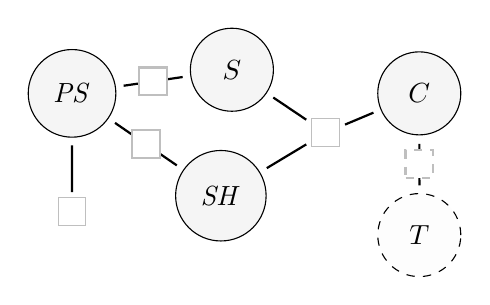
\begin{tikzpicture}[center base, xscale=1.4,
					fgnode/.append style={minimum width=3em}]
					\node[factor] (prior) at (1.65,-1) {};
					\node[factor] (center) at (3.95, 0){};
					
					\node[fgnode] (PS) at (1.65,0.5) {$\mathit{PS}$};
					\node[fgnode] (S) at (3.1, 0.8) {$S$};
					\node[fgnode] (SH) at (3.0, -0.8) {$\mathit{SH}$};
					\node[fgnode] (C) at (4.8,0.5) {$C$};
					
					\draw[thick] (prior) -- (PS);
					\draw[thick] (PS) --node[factor, fill=white](pss){} (S);
					\draw[thick] (PS) --node[factor, fill=white](pssh){} (SH);
					\draw[thick] (S) -- (center) (center) -- (SH) (C) -- (center);
					
					%					\node[dpadded, fill=blue] (1) at (2.5,-2) {1};
					%					
					%					\draw[blue!50, arr] (1) -- (prior);
					%					\draw[blue!50, arr] (1) -- (center);
					%					\draw[blue!50, arr] (1) -- (pss);
					%					\draw[blue!50, arr] (1) -- (pssh);
					
					
					\node[fgnode, fill opacity=0.02,dashed] (T) at (4.8, -1.3) {$T$};
					\draw[thick,dashed] (T) -- node[factor, fill=white]{}  (C);	
			\end{tikzpicture}}
        ~\vrule~
		% \end{subfigure}
		% \begin{subfigure}{0.5\linewidth}\centering
		\scalebox{1}
        {
			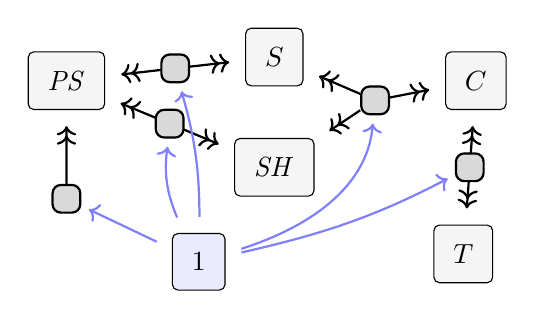
\begin{tikzpicture}[center base, xscale=1.6,
                newnode/.style={rectangle, inner sep=5pt, fill=gray!30, rounded corners=3, thick,draw}]
				\node[newnode] (prior) at (1.65,-1) {};
				\node[newnode] (center) at (4.1, 0.25){};
				
				\node[dpadded] (PS) at (1.65,0.5) {$\mathit{PS}$};
				\node[dpadded] (S) at (3.3, 0.8) {$S$};
				\node[dpadded] (SH) at (3.3, -0.6) {$\mathit{SH}$};
				\node[dpadded] (C) at (4.9,0.5) {$C$};
				
				\draw[arr, ->>, shorten <=0pt] (prior) -- (PS);
				\draw[arr, <<->>] (PS) --node[newnode](pss){} (S);
				\draw[arr, <<->>] (PS) --node[newnode](pssh){} (SH);
				\draw[arr, <<-, shorten >=0pt] (S) -- (center); 
				\draw[arr, <<-, shorten >=0pt] (SH)-- (center); 
				\draw[arr, <<-, shorten >=0pt] (C) -- (center);
				
				\node[dpadded, fill=blue] (1) at (2.7,-1.8) {1};
				
				\draw[blue!50, arr] (1) -- (prior);
				\draw[blue!50, arr] (1) to[bend right=30] (center);
				\draw[blue!50, arr] (1) to[bend right = 5] (pss);
				\draw[blue!50, arr] (1) to[bend left = 10] (pssh);

				
				\node[dpadded] (T) at (4.8, -1.7) {$T$};
				\draw[arr, <<->>] (T) -- node[newnode](tc){}  (C);	

				\draw[blue!50, arr] (1) to[bend right = 10] (tc);
		\end{tikzpicture}}
		% \end{subfigure}
	
	\caption{
%oli20: oops garbled. Fixing.
% The conversion from a PDG to a factor graph to factor
% graph, and vice versa, as defined in \Cref{def:fg2PDG}. The
%joe18: still garbled
%Conversion of the PDG in \cref{ex:smoking} a PDG to a factor graph
Conversion of the PDG in \cref{ex:smoking} to a factor graph
according to \cref{def:PDG2fg} (left), and from that factor graph back
to a PDG by \cref{def:fg2PDG} (right). 
%oli20:
%joe18
%In the later,
In the latter,
%joe17
%blue edges carry the (renormalized) cpds corresponding to the
%joe18: what does ``renormalized'' mean here?  Why did the cpds have
%to be renoormalized
%blue edges are associated with the (renormalized) cpds corresponding to the
blue edges are associated with the cpds corresponding to the
%joe17: what's a product node?  This is very mysterious, and needs to
%be expanded a bit.
%oli20:
% original factors, and product nodes 
original factors, each leading to a new node $X_J$ (displayed as a
%joe18
%smaller darker rectangle) whose values are joint settings the
smaller darker rectangle) whose values are joint settings of the
variables connected to the factor $J$. 
%oli20:
%	are inserted for every edge.
} 
	\label{fig:fg2PDG}
\end{figure*}

%joe1: rewrote
%Surprisingly, despite garbling the structure (see
%\Cref{fig:fg2PDG,fig:fg-intro-examples}), when we fix $\gamma=1$, the
%two operations preserve most of their semantics.
PDGs are directed graphs, while factors graphs are undirected. The
map from PDGs to factor graphs thus loses some important structure.
As shown in
%joe17: I get problems when I latex this.  It says ``As shown in
%Figures 8 and 9 in Figure 9''. Moreover, the actual figure is Figure 4.
%oli20: another problem with comments... should be fixed now. 
\vfull{
    \Cref{fig:fg2PDG,fig:fg-intro-examples}
}%\end{vfull}
\Cref{fig:fg2PDG},
%joe11
%the mappings can change the graphical structure signfiicantly.
the mappings can change the graphical structure significantly.
%oli12: no \alphas, so we have something slightly different is true.
% Nevertheless, if we take $\gamma=1$,
Nevertheless, in the case where every weight is the same,
%joe18: why do we have to say this
%and equal to $\gamma$,
%oli19: because the process is not involutive, I'm changing the wording
% then the factor graph and the associated PDG have the same semantics.  
then both conversions preserve the semantics. 

\commentout{
%oli9: this holds more generally, illustrating that PDGs can carry factor graph data regardless of \theta, \beta.
	\begthm{prop}{prop:fg-pdg-lossless}
		$\Phi \circ \PDGof = \mathrm{Id}_{\text{FG}}$. That
		is, if $F$ is a factor graph, then
		$\Pr_{\Phi(\PDGof{F})} = \Pr_F$. 
	\end{prop}
}

% \begthm{theorem}[restate=thmpdgisfg]\label{thm:pdg-is-fg}
\begthm{theorem}{thm:pdg-is-fg}
%oli20: ok let's be more careful. What is 'gamma'?
% If $\dg M$ is a PDG with $\beta_L = \gamma$ for all 
%joe18: I actually thought it was fine before, but I'm OK with the
%following slight reweroding
%If $\dg M$ is a PDG, and $\gamma$ is a number such that $\beta_L\!
If $\dg M$ is a PDG such that for some $\gamma >0$, we have that $\beta_L\!
= \gamma$ for all  
%oli12 line shave
%edges
 $L$, then
%oli20: we're now using subscripts. Also, swapping order so the conclusion
% is read in the direction we're emphasizing. Spacing also.
% $\gamma \mathcal G_{\Phi(\dg M)} = \bbr{\dg M}_{\gamma}$ and
% $\bbr{\dg M}_{\gamma}^* = \{\Pr_{\Phi({\dg M})} \}$.
%joe18*: this is problematic given your current notation.  \G needs to
%subscripts, and so does \Pr.
$\bbr{\dg M}_{\gamma} = \gamma\,\mathcal G_{\Phi_{\dg M}}$ and
$\bbr{\dg M}_{\gamma}^* = \{\Pr_{\Phi_{{\dg M}}} \}$.
% $\kldiv{\mu}{\Pr_{\Phi(\dg M)}} = \bbr{\dg M}_{1}(\mu)$
	% In particular, $\Pr_{\Phi(\dg M)} = \bbr{\dg M}_*^{\gamma := 1}$
\end{theorem}
% \begin{theorem}[restate=thmfgispdg]\label{thm:fg-is-pdg}
\begthm{theorem}{thm:fg-is-pdg}
%oli20:
% For a factor graph $\Phi$,
Given a factor graph $\Phi$, 
%oli20: \gamma is undefined; re-wording and precisifying:
% such that $\theta_J = \gamma$ for all factors $J$,
and a constant vector $\kappa = \{ k \}_{J \in \cal J}$ for some fixed $k$, then
we have that
% for any joint distribution $\mu$ on $\V(\mathcal X)$, we
        % have $\kldiv{\mu}{\Pr_\Phi} = \bbr{\PDGof{(\Phi)}}_{1}(\mu)$ 
%joe8: again
%oli10: adding back in
%joe9
        %	$\gamma \mathcal G_\Phi = \bbr{\PDGof{(\Phi)}}_{\gamma} + k$
        %        where $k$ is a constant, and in particular, 
%oli20: fixing it all at once:
	% $\gamma \mathcal G_\Phi = \bbr{\PDGof{\Phi}}_{\gamma} + k$  
	% for some constant $k$, so
	% $\bbr{\PDGof{\Phi}}_{\gamma}^* = \{\Pr_{\Phi} \}$. 
%joe18: missing \kappa, I think
%$\mathcal G_{\Phi, \kappa} = \nicefrac{1}{k}\bbr{\PDGof{\Phi}}_{k} + C$  
$\mathcal G_{\Phi, \kappa} = \nicefrac{1}{k}\bbr{\PDGof{\Phi,\kappa}}_{k} + C$  
for some constant $C$, so
	$\Pr_{\Phi, \kappa}$ is the unique element of $\bbr{\PDGof{\Phi,\kappa}}_{k}^*$. 
\end{theorem}
%oli20: general versions for whole exponetial family
\noindent\contentious{
%joe18*: rewrote.  Assuming we keep this, the real question is where
%we introduce \alpha.  If we introduce it at the beginning, then we
%need to include it in the BN theorem and were really should give more
%intuition (which we'll have a hard time agreeing on, based on past
%history), although perhaps we can get away with saying that we'll
%just use it in a technical way.  Obviously, if we include it, we
%shold get rid of Theorems 4.2 and 4.3, and just use the stronger version. 
%These theorems above are actually quite restrictive:
%	both \cref{thm:pdg-is-fg,thm:fg-is-pdg} require that the
%	confidences be uniform,  
	% and even then only offer a correspondence for a specific value of $\gamma$, which makes it impossible to even consider our limit.
These theorems are quite restrictive:  Theorem~\ref{thm:pdg-is-fg}
applies only to PDGs where all the uncertainties $\beta_L$ are
identical, while Theorem~\ref{thm:fg-is-pdg} applies only to factor
graphs where all weights $\Theta_J$ are identical.  We can generalize
Theorem~\ref{thm:pdg-is-fg} slightly to the case where the ratio of
$\alpha_L$ to $\beta_L$ is a constant.
			
	\begthm{theorem}{thm:pdg-is-fg2}
%joe18
%If $\dg M$ is a PDG, and $\gamma$ is a number such that
If $\dg M$ is a PDG such that for some $\gamma >0$, we have that
	$\beta_L = \alpha_L \gamma$ for all  
	%oli12 line shave
	%edges
	$L$, then
	$\bbr{\dg M}_{\gamma} = \gamma\,\mathcal G_{\Phi_{\dg M}} $ and
	$\bbr{\dg M}_{\gamma}^* = \{\Pr_{\Phi_{\dg M}} \}$.
	 	% $\kldiv{\mu}{\Pr_{\Phi(\dg M)}} = \bbr{\dg M}_{1}(\mu)$
		% In particular, $\Pr_{\Phi(\dg M)} = \bbr{\dg M}_*^{\gamma := 1}$
	\end{theorem}
	% \begin{theorem}[restate=thmfgispdg]\label{thm:fg-is-pdg}

%joe18* unless I'm missing something, you need to redo Definition 4.3
%to explain how to add the \alphas.  Will you add them in such a way
%that the ratio of \beta_L to \alpha_L is constant?  If so, we can say
%that because the construction made it a constant, the following result holds.
%If the updated Definition 4.3 allows some flexibility in
%choosing \alpha and \beta, then this would reqire more work.

	\begthm{theorem}{thm:fg-is-pdg2}
	%oli20: we got to remove the condition!
For every factor graph $\Phi$, and EVERY vector $\theta$ over $\cal J$ 
	%, and EVERY $\gamma >0$
	we have that
	% for any joint distribution $\mu$ on $\V(\mathcal X)$, we
	        % have $\kldiv{\mu}{\Pr_\Phi} = \bbr{\PDGof{(\Phi)}}_{1}(\mu)$ 
	%joe8: again
	%oli10: adding back in
	%joe9
	        %	$\gamma \mathcal G_\Phi = \bbr{\PDGof{(\Phi)}}_{\gamma} + k$
	        %        where $k$ is a constant, and in particular, 
		$\mathcal G_\Phi = \nicefrac1{\gamma} \bbr{\PDGof{\Phi,\theta}}_{\gamma} + C$  
	for some constant $C$, so
	   $\Pr_{\Phi, \theta}$ is the unique element of $\bbr{\PDGof{\Phi,\theta}}_{\gamma}^*$. 
	   % Moreover, $\Pr_{\Phi, \theta} = \bbr{\PDGof{\Phi,\theta}}^*$.
	\end{theorem}

%joe18: cut from here.  Once we fix the second theorem, the relevant
%discussion should go before the theorem
%	\cref{thm:pdg-is-fg} still has a retriction, but if we can
%        choose the values of $\alpha$ (or alternatively $\beta$), we
%        can get the result to apply for arbitrary values of $\gamma$
%        and $\beta$ (resp. $\alpha$). \Cref{thm:fg-is-pdg2} is
%        substantially stronger than its counterpart: it shows that
%        PDGs in which the quantitative and qualitative certainties are
%        fused ($\alpha_L = \beta_L$) completely adopt the semantics of
%        factor graphs and their exponential families, for $\gamma =
%        1$.\footnotemark 
%joe18*: This is the point; you have to explain how the tranlsation
%works in the presence of \alpha!
%\vcontentio{\footnotetext{The result can be achieved for arbitrary
%	$\gamma \neq 1$, if we are willing to set $\alpha$ based on
%	$\gamma$ in our translation of factor graphs to PDGs.}} 

%oli19:
% Justification for both theorems is provided by rewriting
%joe18*: We need to add a proof for this result in teh appendix.
%The truth of \Cref{thm:fg-is-pdg,thm:pdg-is-fg} may be seen
%intuitively by rewriting 
The key step in preoving \Cref{thm:fg-is-pdg,thm:pdg-is-fg}
(and in the proofs of a number of other results) involves 
rewriting  
$\bbr{\dg M}_\gamma$ as follows: 
\begin{prop}[restate=prop:nice-score,label=prop:nice-score]% \label{}
% \begin{restatable}{prop}{propnicescore}\label{prop:nice-score}
 Letting $x^{\mat w}$ and $y^{\mat w}$ denote the values of
  $X$ and $Y$, respectively, in $\mat w \in \V(\dg M)$, 
we have 
\begin{equation}\label{eq:semantics-breakdown}
\begin{split}
%joe17*: Now that I look at it again, this is horrible notation, and
%it confused me for a whle.  When we write E(X), X is a random
%variable.  So what random variable are you taking the expectation of
%Look at the last term.  You wrote \mu(w), but that's not a random
%variable.  (I suspect that there's a typo here and it should
%be \mu(\mat w).  But, in any case, that's a value, not a random
%varaible (which is a function.  I just got rid of the E and corrected
%the typo, so it least now it's mathematically correct.
%oli20: Hmm. I'm willing to accept the change, but I don't buy the
%argument. Is there something wrong with regarding $\mu(\mat w)$ as a
%random variable which depends on \mu? It clearly is a function from
%worlds to reals. Convention, exepctation is quite common in such
%contexts in information theory, and quite intuitive (for instance,
%the entropy = "expected surprise" relies on this). As a matter of
%consistency, you should be aware that we do a very similar thing in
%the definition of Inc: there's an expected  divergence
%from \mu(Y|x). This kind of term is common, the expectation is the
%standard way to write it.
%joe18: you're right; we do it there, and it's a bad abuse of notation
%there too.  Probabilists have this unfortunate habit of using what I
%find terribly confusing notation.  I always feel forced to unpack
%it.  How many people who read this even realize that a random
%variable is not a variable and is not random, but is a function.  I
%would actually prefer to rewrite Definition 3.2 this way as well.  I
%think it would make it clearer to get rid of the expectation.  I
%think it make things clearer to get rid of it.
%oli20: I changed the spacing some so your version looks better. I
%still prefer the expectation but if you're not swayed by the above I
%won't say anything furhter. 
%joe17
% \bbr{\dg M}(\mu) =  \E_{\mat w \sim \mu}\! \Bigg\{
\bbr{\dg M}(\mu) =  \!\!\!\sum_{\mat w \in \V(\dg M)} \!\!\! \mu(\mat w) \Bigg\{
 \sum_{ X \xrightarrow{\!\!L} Y  }
\bigg[\,
    \color{gray}\overbrace{\color{black}
      \!\beta_L \log \frac{1}{\bp(y^{\mat w} |x^{\mat w})}
%	}^{\color{gray}\smash{\text{log likelihood}}} + \\[-0.5em]
	}^{\color{gray}\smash{\mathclap{\text{log likelihood / cross entropy}}}} + \\[-0.5em]
    \color{gray}\underbrace{\color{black} 
(\contentio{$\alpha_L$}\gamma - \beta_L ) \log \frac{1}{\mu(y^{\mat w} |x^{\mat w})} 
	}_{\color{gray}\smash{\mathclap{\text{local regularization (if $\beta_L > \gamma$)}}}}\bigg] - \underbrace{\color{black}
%joe17
%\gamma \log \frac{1}{\mu(w)}
\gamma \log \frac{1}{\mu(\mat w)}
	}_{\color{gray}\smash{\mathclap{\text{global
        regularization}}}}\color{black} \Bigg\} .
\end{split}
\end{equation}
\end{prop}
%joe17*: sorry; this isn't claer to me at all.  
%assume that $\beta_L = \theta_L$.  But we did that, so that's not so
%bad (although you should say it). Second, we get, the last term
%becomes \gamma H(\mu), so it only matches the free energy if \gamma =
%-1.  Finally, why should p_L(y^W | x^w) = \phi_L(x_J) (even if we
%assume that \phi = p_L.
%  Part of the problem is that you wronte in
%the w  I think what you mean is the E(\gamme \log(1/\mu)
%= \sum_\oemga \gamma \mu(w)/log(\mu) = = H(\mu).  But then ou're
%still out by a factor of -\gamma.
%oli20: A factor of + \gamma, but point taken. I guess it's standard
%to effectively 
% fix \gamma=1 for factor graph because the ratio of the \theta's to the entropy term is
% the only thing that matters, so one can fix that scale to 1.
%joe18: it may be standard, but not everyone knows it (I didn't).
%  I've rewritten it so it's more correct. 
%	The first and last terms of \eqref{eq:semantics-breakdown} are precisely
%	$\mathcal G_\Phi$ for $\phi = \bp$.  
%joe18
%For any fixed $\gamma$, the first and last terms
For a fixed $\gamma$, the first and last terms
of \eqref{eq:semantics-breakdown} are equal to a scaled
%joe18: in what sense is it equivalent?  
%(which is essentially equivalent)
%joe18*: I'm confused.  This statement seems technically incorrect to
%me, on  two counts.  First, you would have to
%multiply the first term by \gamma (there is no \gamma factor
%currently in the first term); second, for the last term, the factor
%is -\gamma, not \gamma.  
version of the free energy, $\gamma\mathcal
G_\Phi$, for $\phi_J = \bp$ and $\theta_J
= \nicefrac{\beta_L}{\gamma}$.  
%oli19
% Thus, if we assume that $\phi = \bp$ and in addition assume that each
%oli20: edit for flow
% Furthermore, if each $\beta_L = \gamma$, the local regularization term disappears, so we get 
%joe18
%If in addition, each $\beta_L = \contentio{$\alpha_L$}\gamma$,
If, in addition, $\beta_L = \contentio{$\alpha_L$}\gamma$ for all
edges $L$, then
the local regularization term disappears, giving us
%oli20:
% an exact correspondence with $\mathcal G_\Phi$%
the desired correspondence. 

%oli20: paragraph break + signposting
%joe18*: cut this; see below for why
\commentout{
We now explain how the middle term may be viewed as a ``local'' regularization,
and why including such a term is necessary for the semantics to 
%joe18*: I find this statement very confusing.  Why shouldn't we take
%them seriously?  And they *are* assertions about probability, no
%matter how we  take them.  Most importantly of all, I see no way in
%which this example tells me anything about how I shoudl view p.  It
%shows potential probablems with the factor graph (which is what I
%believe it was intended to do).  Some signposting would be useful, but I find
%this completely unhelpful.  We had some text here which you seem to
%have cut, rather than commenting it out.  I though the text was fine,
%and I'm reinstating it.  (Also, please don't just cut text.)
%take our cpds $\mat p$ seroiusly, as assertions about probability%
view our cpds $\mat p$ as assertions about probability%
% (instead of viwing them as each contributing to a badness, as factor graphs do)
. 
%oli20: pulled example from the end of the document.
}

%joe18*: reinstating some material from before, with slight rewriting.
\Cref{eq:semantics-breakdown} also makes it clear that 
taking $\beta_L = \alpha_L \gamma$ for all edges $L$ is
essentially necessary to get \Cref{thm:pdg-is-fg,thm:fg-is-pdg}.
If this equality does not hold, then we can get some 
some strange
behavior in factor graphs trying to capture the same phenomena as
PDGs, as the following example shows.

\begin{example}\label{ex:overdet}
Consider the PDG $\dg M$ containing just $X$ and $1$, and two edges
$p, q: 1 \to X$.
%joe8:
(Recall that such a PDG can arise if we get different information about the
probability of $X$ from two different 
%oli19:added, otherwise this is a reasonable inference
% but not independent
%joe17: I don't understand.  Such a PDG can arise whether or not the
%sources are independent.  There is no inference going on here!  If
%you want to say something about non-independence, it should go
%somewhere else.
%oli20: I'm not trying to say anything about independence, but we want the
%example to be a clear illustration of what PDGs buy you. If I thought the
%sources were independent, I would be justified in combining 0.7 and 0.7 to get
%0.85. I find the example to be more powerful if we explicitly state that we
%don't know them to be independent, so we cannot make this inference. Thoughts?
%joe18: This is not the place to discuss these issues.  We're just
%trying to make a point about factor graphs having strange behavior.
%The issue of combining .7 and .7, and possibly getting .85 needs
%*much* more discussion; this is not the place to do it.
sources; this is a situation we
certainly want to be able to capture!)
Consider the simplest situation, where $p$ and $q$ are both associated
with the same distribution on $X$%
%oli20: added next line
%joe18:
%	, as the same certainty $\beta_p = \beta_q = 1$.
; further suppose that the agent is certain about the distribution, so
$\beta_p = \beta_q = 1$.
%joe18*: what abou \alpha?  If we introduce it, we have to say
%something about it here.
For definiteness, suppose that
$\V(X) = \{x_1,x_2\}$, and
that the distribution associated with both edges is $\mu_{.7}$, which ascribes
%joe9: slowing down.
%probability $.7$ to $x_1$, then  $\bbr{\dg M} = \{\mu_{.7}\}$,
%while it can be shown that 
probability $.7$ to $x_1$. Then, as we would hope  $\bbr{\dg M}^* =
\{\mu_{.7}\}$; after all, both sources agree on the information.
However, it can be shown that 
%oli20: some M's escaped. Added msising subscript.
% $\Pr_{\Phi{{\dg M')}}} = \mu_{.85}$, so  $\bbr{\dg M'} = \{\mu_{.85}\}$.
%joe18: there's a typo here: I wrote what I thought you intended
%$\Pr_{\Phi{{\dg M)}}} = \mu_{.85}$, so  $\bbr{\dg M}_1^* = \{\mu_{.85}\}$.
%joe18*: this arguably also shows the problem with the \bbr{\dg M}_k^*
%semantics when k \ne 0.  We should say something about that.
$\Pr_{\Phi_{{\dg M)},1)}} = \mu_{.85}$, so  $\bbr{\dg M}_1^* = \{\mu_{.85}\}$.
\end{example}

%joe11*: is this what you mean?  Why is there only one such world?
%optimal distribution would put all mass on the single best world; to
%oli13: It's not guaranteed to be unique, but all mass is concentrated
% on those worlds(s) which maximize the function. Added plural.
%oli19: rewrote
% If we had included only the likelihood term (the first one), 
% an optimal distribution would put all mass on the worlds of maximum likelihood. 
%joe17*: I don't undrstand why you made these changes.  How do you know
%that there's a unique world of maximum likelihood?
%oli20: it's not litterally true, but overwhelmingly likely and I don't want to
% complicate the story unnecessarily. See the below.
%the best distribution would put all mass on the highet likelihood world. 
%oli20: commenting out, see discussion + replacement below.
% the best distribution would put all mass on the worlds with maximum likelihood.
%joe17: I really don't like ``devoid of unceratinty''!  Moreover, if
%there isn't a unique world of maximum likelihood, why is there no
%uncertainty?  
%oli20*: while there may be multiple, any "uncertainty" is extremely fragile. 
% With any real data, there is a unique best world with probability 1.If we add
% epsilon noise to every cpt entry, there is a unique best world with probability 1.
% In the same vein: the only way it is possible for an interior point to have any probability at all, is if the product of the factors is is the constant function. 
%oli20: A simple example: a binary variable X, with an edge from 1 and an unconditional distribution % p(X=1) = 0.5 + \epsilon.  But X=1 is the only maximum likelihood world, so the optimal distribution is % the one that places all mass on X=1.  Taking this distribution seems hugely overconfident, and is totally in conflict with the uncertainty in the cpt. This is essentially what is hapepning in a factor graph. 
%oli20: trying again.
%joe18: this is not helpful  
%The log likelihood term
%%, which is as the cross entropy, 
%is the only term that makes use of the cpds.
%joe18*: in what sense is it the most important?
%so in some sense it is the most important.  
%joe18*: Sorry, I can't make any sense of the next sentence.  In what
%sense are the distributions miscalibrated?
%On its own, however, the distributions it selects are badly
%miscalibrated, placing all mass on worlds with the very highest
%likelihood.
%joe18*: the best distance by what metric?
%For instance, the best distribution in \cref{ex:overdet}
%by this metric is $\mu_{1.0}$, even if only link $p$ were given ---
%which is in direct conflict with $p$ itself.  
%Such a distribution is devoid of uncertainty, which usually is in direct
%conflict with the data of the cpds $\mat p$.
%joe17: What issue is it resolving?  How is it resolving it?
%oli20: hopefully clearer now; I'm uncommenting and expanding.
%joe18*: I'm afraid it's not at all clear, and I still have no idea
%what issue is being resolved.
%A factor graph essentially resolves this issue by
%also including the final term,
%oli20: added
%joe18*: Sorry, I can't make any sense of this.  What does it mean to
%``properly balance'' something.  How can ou tell if it's ``properly
%balanced''.  
%which imposes a cost for uncertainy. For the PDG consisting of only
%$p : 1 \to X$ from \cref{ex:overdet}, this results in $\bbr{1 \to
%p}^* = p$. As we have seen, adding $q$ . It seems that as long as our
%regularization term remains agnostic to the number of links in the
%graph, and which nodes they attach to, it cannot properly balance the
%likelihood so that the cpt is satisfied.    

%joe17: I don't understand the next sentence.  I have no idea of the
%sense in which local unceratinty ``offset'' local energy, and have no
%idea what it would mean to do so.  I tried to write what I
%thought you intended in a less mysterious way
%PDG semantics may be viewed as extending factor graphs with ``local
%uncertainty'' to offset each local energy.
%joe18*: The next sentence should go earlier, after we've talked about
%that first and last terms of (5) captring the free energy.
%The scoring function that we use for PDGs can thus be viewed as
The scoring function that we use for PDGs can be viewed as
%oli20: added \theta. Also, we're not naming this term, we're just describing it. Its name is conditional entropy.
% extending ${\mathcal G}_{\Phi,\theta}$ by including what we have called the local
extending ${\mathcal G}_{\Phi,\theta}$ by including
%joe18
%a \emph{local} regularization term.
the local regularization term.
%oli20: more analogy.
As $\gamma$ approaches zero,
%joe18: it's not the strength, but the importance
%the strenth of global regularization
%drops and the strength of local regularization increases. 
the importance of the global regularization terms decreases relative
 to that of the local regularization term.
%joe17*: I can't even parse the rest of this, let alone understand it.
%I just cut it.
%As $\gamma \to 0$, these local terms dominate.
%, and the semantics correspondingly that a distribution $\mu$ has the
%appropriate amount of uncertainty at the target of each edge, while
%demoting the 
%preference for entropy on other variables (which the does not know about) to an
%infinitessimal tie-breaker.

%joe11*: why do we want to express uncertainty?   What is it
%uncertainty about.  I'm trusting you that ``regularization'' will be
%meaningful in this context to others.  It's certainly not meaningful
%to me. You have the space to add a sentence of clarification.
%oli13: "Uncertainty" was maybe not the best word choice. Let's try this:
% to capture $\bbr{\dg M}_\gamma(\mu)$, we need to include 
%joe13*: this doesn't make sense to me.  Where did overfitting come
%from?  We're not doing machine learning?  Since you haven't told me
%the objective function, so to speak, I find this worse than useless.
%It makes me think of things that ought to be irrelevant. At a
%minimum, to include them, you must explain the goal (i.e., give some
%intution!).  
%to avoid overfitting these particular distributions, we need to include 
%\emph{regularization terms} \todo{cite}.  
%oli15
% the regularization terms are needed to capture the inconsistency and
% information deficiency of $\mu$ relative to ${\dg M}$.
%joe14: I put ``regulararization'' in quotes
%the regularization terms are thus necessary to model uncertainty.
%You need to say something about how, although they're not
%regluarization terms as the term is used in the ML community (since
%we are *not* doing machine learning), they have some of the same spirit.
%joe15*: Why are regularization terms necessary to model uncertainty?
%All that you can say is here is that they're necessary to capture
%this particular socirng function
%oli17*: No, this is much weaker than what I want to say. These terms
%are  necessary to have an optimal distribution $\mu$ that is not a
%point mass on a particular world. 
%oli17: Unsure if helpful, but the thermodynamic analogy is
%temperature=0 Kelvin, 
% so that everything is in its very minimum energy state, and the distribution of possible
% configurations is a point mass on the single best one. 
%oli17: Again, the point is: if we want it to even be possible for the minimum
% of this function to be a non-degenerate distribution (i.e., one with uncertainty),
% then we need the regularization terms. 
%oli17: rewrote more explicitly, in the hopes that this was convincing.
%
%the ``regularization'' terms are thus necessary to model uncertainty.
% the ``regularization'' terms are thus necessary to capture $\bbr{\dg
  % M}_\gamma$. 
%joe16*: Cut.  I do not understand what this means, or why it's
%important.  This hurts far more than it helps.
%the ``regularization'' terms are thus necessary for these
%distributions to have any uncertainty. 
%oli19: rewriting.
% By contrasting equation
% \eqref{eq:semantics-breakdown} with the expression for $\mathcal G_\Phi$, we see
% that, although both $\theta$ and $\beta$ are measures of confidence, the way
% that a factor graph varies with $\theta$ is quite different from the way a PDG
% varies with $\beta$. 
%joe17: Cut this.  I 
%The fact that the local term varies with $\beta_L$ has important
%modeling consequences. 

Although both $\theta$ and $\beta$ are measures of confidence, 
%joe17
%the way $\theta$ that a factor graph varies with $\theta$
the way that a factor graph varies with $\theta$ 
is quite different from the way a PDG
varies with $\beta$. 
%joe17*: I don't undersatnd teh rest of this.  I couldn't see anywhere
%in the example where these points were illustrated.  Indeed, the
%exampe doesn't mention \beta at all.  If you could rewrite the exmple
%to illustrate these points, we might consider reinstating this.
%oli20: fair enough, reinstated and added missing details. 
%joe18*: I still can't make sense out of any of this.  As an aside,
%this is *not* what I asked you to do.  I asked you just to focus on
%the technical material, which is all I was (and am) comfortable with.
%$\theta_J$ controls the strength of the potential associated to $J$;
%joe18*: I don't understand this.  Why does increasing one
%terms \theta_J for a specific J, make distributions more
%deterministic.  If you increase all of them, I can see how it wuld
%make distributions more determininstic, but only if all the ffactors 
%were different numbers.  But why do we are about this?  We're writing
%a paper about PDGs.  What does this tell us about PDGs.
%increasing it results in optimal distributions which are more
%deterministic.  
%oli20: added
%joe18*: I have no idea how a generaic atatement about properties. I
%would *strongly* prefer to return this to its previous state (modlo
%the technical concerns I've raised).
%of \theta_J could follow from an Example.  But even if you meant that
%Example 5 illustrates your point, I can't see any way in which you've
%argued that doubling J makes things more deterministic.  The next
%sentence just feels like a complete non sequitur.  
%This follows from \cref{ex:overdet} the fact that doubling $\theta_J$
%is equivalent to duplicating factor $J$. By contrast, $\beta_L$
%controls both the likelihood and the local uncertainty together: as
%described in our motivation for $\Inc$, increasing the reliability of
%$\beta$ in a PDG increases the cost of failing to match the given cpd.  
%\\\contentious{
The behavior in \cref{ex:overdet} also sheds some light on the nature of $\alpha$.
Because a factor graph fuses $\alpha_L = \beta_L$, adding a new edge effectively doubles both (it doubles $\theta_L$). If one believes that both $p$ and $q$ are from independent sources, and thus constitute separate qualitative determinations of $X$, then effectively doubling $\alpha_p$ is appropriate. If, on the other hand, you merely have two distinct sets of observations which agree, and have no reason to believe they are independent or have anything to do with the causal structure of the world, then effectively doubling $\alpha_p$ is not appropriate.  
}
%
%joe13*: the equation says nothing abut \theta.  This is even more
%confusing because in the tranlsation you take \beta_L = \theta_L.  My
%preference would be to ut the rest of the paragraph, although I didn't
%do it.  I think it hurts more than helps.
%\eqref{eq:semantics-breakdown} shows further that, although
%oli15
% \eqref{eq:semantics-breakdown} helps show  that, although
%oli12: added the technical details and fused with next sentence
%joe11*: typo, I assume.  If not, then it's unclear
%For a factor graph, $\beta$ controls the importance of the likelihood
%term, while in a PDG it also increases the strength of the local
%oli13: you're right. This enables further simplification
% For a factor graph, $\theta$ controls the importance of the likelihood
% term, while in a PDG, $\beta$ it also increases the strength of the
%joe13: I don't know what ``jointly controls'' means.  After changing
%the next few lines, I cut them.   It's true that \beta affets both
%the likelihood term and the local regularaization term, but I don't
%wee why that makes it different from theta; there is no theta in the
%equation above
%oli15: I've reverted because the story makes more sense with this in than out. 
% It's true and I think it won't be too difficult to follow from the equation.
%%$\beta$ jointly controls the importance of the likelihood and local
%oli15 modified
%joe14*: In what sense does it balance them?  I'm lost.  If you say
%``affects'' it's fine.  If not, you must explain what ``balance'' means.
%oli16: the strength of the regularization must match the strength of
%the likelihood. Only then is the function minimized by the cpd on the
%edge, rather than a more deterministic one (if the former is
%stronger) or a more random one (if the latter is stronger). 
    % $\beta$ balances the likelihood and local
    % regularization terms [[REWRITE]], while 
    % $\theta$ affects only the former.
%oli16: rewritten so that now it is clear, but much too long. I like my shortening above,
% and do not think it needs anything else, but I'll let you shorten this one as you like. It also double-covers material from the next sentence.)
%joe15*: Sorry; it is *not* clear (at least, not to me).  I don't know
%what it means that they ``remain balanced''.  I also don't like the
%use of terms of agency (``controls'').  Are you saying anything other
%than \beta affects the difference between the terms.  Is that what
%balance is supposed to mean?  If so, it's an awfully complicated way
%of saying it.  If not, what is it saying that's different?  I cut
%most of it.  I think that what you wrote is a net negative; in
%expectation, it will hurt more than it will help.  Do NOT
%make further changes without discussion (other than correcting typos)
%$\beta$ simultaneously controls both the local likelihood and local
%regularization terms, so that the two remain balanced, and making a
%link more or less random never does better than exactly matching the
%cpt.  
%oli17: \beta preserves the ratio between the first and second 
% terms (in the limit as \gamma -> 0)
%joe16: As a technical matter, I don't see why this is true.  I don't
%see in what sense \beta preserves anything.  It's just a number that
%you miltiply the difference between the terms by.  
%oli17: and the cpds that that optimize it remain the same.
%joe16: The same as what?  I'm totally lost
%oli17: This is very different from just increasing the strength of the 
% likelihood because it makes things more determinisitc. I maintain that this
% is a critical point, but I will not modify the text here to make it until we
% agree...
%joe16: good.  I truly have no idea what you said above, and I
%strongly suspect that I would not understand anything you tried to
%say here.
%oli19: I don't need this anymore either
%joe17: reinstated, because I cut what you added
%oli20: removed again. I don't think this says very much, and I've tried
% to address your concerns again.
	% In (\ref{eq:semantics-breakdown}), 
	% $\beta$ affects the difference between the local likelihood and
	% local regularization terms; on the other hand, in $\mathcal G_\Phi$,
	% $\theta$ affects only the likliehood.
% %oli17
% $\theta$ affects only the likelihood.
%$\theta$ only controls the likliehood, and so as it
%increases the benefits of reporting an uncertain distribution fade as

\Cref{eq:semantics-breakdown} also makes it clear that 
%joe11*: what does ``on the smae scale'' mean?   Why say something
%mysterious when you can say it clearly
%oli13: This is weaker than what I meant to say. The point is to get the result,
% you need $\gamma$ to be small enough; we cannot approximate  with small
% gamma if it is fixed to the scale of the $\beta's$. This is fine though.
%fixing $\gamma$ on the same scale as $\beta$ is 
taking $\beta_L = \contentio{$\alpha_L$} \gamma$ for all edges $L$ is
essentially necessary to get \Cref{thm:pdg-is-fg,thm:fg-is-pdg}.
However, the analogue of \Cref{prop:consist} does not hold
in general for such choices, leading to some arguably unacceptable
% strange
behavior in factor graphs 
%oli19
%joe17: No!  We've never talked about epistemic state before.  Now is
%not the time to start.
trying to capture the same phenomena as PDGs.
%trying to capture epistemic state.

%joe9: cut; folded some material into the next section
%oli20: I rewrote this section and brought it up in case 
%joe18: I commented it out again, after making minor changes.  Nothing
%in what you've written explains the connection between PDGs and
%directed factor networks.  THere's no point in giving a (not
%particularly useful) introduction to directed factor graphs.  We're
%not writing a paper about factor graphs.  If you have something
%useful to say about the connection between diredcted factor graphs
%and PDGs (e.g, we can prove an analogue of THeorems 4.4 and 4.5 for
%them), then it would be worth saying.  Otherwise, this is a poor use
%of space.
\commentout{

	\subsection{Directed Factor Graphs}
	% Directed Factor graphs \cite{frey2012extending} impose constraints on factor graphs to resolve some of their issues and bring them more in line with BNs, but they have no semantics if the constraints are not satisfied, making them a way of visualizing factor graphs more than a novel modeling tool.
%joe18
%While PDGs can be thought as a loosening the restrictions on
While PDGs can be thought as a loosening of the restrictions on
	Bayesian Networks, 
%joe18
%Directed Factor Graphs \cite{frey2012extending} go the
\emph{directed Factor Graphs} \cite{frey2012extending} go in the
	opposite direction: they  
%joe18: I don't know what ``better-behaved'' means.  Better behaved
%than what?
%extend factor graphs with better-behaved directed edges,
are variant of factor graphs where edges are directed,
	allowing them to represent a larger class of independencies,
%joe18
%including those of Bayesian Networks. Such an directed edge
including those of Bayesian Networks. A directed edge
	indicates that the product of incoming edges normalize to 1,
	an invariant which must be enforced and maintained as the
	model is changed. As a result, directed factor graphs are
	well-suited to visually describing the structure of
	distributions, but less well suited to modelding beliefs that
	change quickly, or could be inconsistent. 
}
%oli20: I got to this a bit late and didn't do as good a job as I wanted, but
%this is the flavor of whwat we can expect. I'm pretty sure the conjecture is
%true, though it won't quite litterally hold for /inconsistent/ dependency
%graphs, because ordered sampling is very hacky. I suspect it does hold if we
%were to eliminate the "ordered" bit of their semantics and randomize th link
%according to $\beta$, which would be a nice result.
%joe18*: commented this out again.  If you can prove your conjecture,
%then it would be worth adding.  Otherwise, it hurts mor than helps.
\commentout{
	\subsection{Dependency Networks}
%joe18
%PDGs are much more closely related to Dependency Networks, or
PDGs are closely related to Dependency Networks, or
DNs \cite{heckerman2000dependency}. 
	The data of a DN is also an unstructured collection of cpds,
        but the cpds are attached to nodes rather than edges, so there
        must be exactly one per
        node.  \citeauthor{heckerman2000dependency} also emphasize the
        benefit of being able to supply arbitrary data in the cpds,
        even if they are inconsistent. Although on the surface PDG and
        DN semantics are quite different (the latter is in terms of an
        ordered Gibbs sampler), it turns out that DNs too are a
        specific case of a PDG.  
%joe18*: It's strange to say ``it turns out'' and then to state a
%conjecture, rather than a theorem.

	\begin{conj}
		If $\mathcal D = (\N, \Ed, \V, \mathcal P)$ is a consistent dependency network with a positive stationary distribution $p^*$ of its sampling procedure, then the PDG $\PDGof{\mathcal D} = (\N, \mathit{merge}(\Ed), \V, $$\mathcal P, \mat 1\contentio{, $\mat 1$})$, then $\bbr{\PDGof{\mathcal D}} = p^*$.
	\end{conj}
	\begin{proof}
		Sketch:  By Theorem 2 of their paper, the stationary point of this procedure is unique, and equal to the only distribution $p$ which both is consistent with the independece assumptions, and also the cpds.  A feq examples strongly suggest thte independece assumptions associated with this structure, are correctly encoded in $\IDef{\PDGof{\mathcal D}}$. This needs to be done more rigorously but I don't expect it to be too bad.
\end{proof}
	
}
%joe9: \end{commentout}
	
	% \todo{more related work if this is the right place to put it.}

%oli8: Removed the two large sections on themodynamics and moved them to the appendix. 
%TODO: I still have to merge the two thermo sections there.

%joe8: This will not make it to the submission.  It's totally
%unrelated to the rest of the paper.  We should definitely write a
%paper on incosnsiency (the one we were originally going to write) but
        %this isn't it
{%\color{blue}        
%joe18*: Oliver, this is a bad idea.  We have a poorly presented
%example instead of a big story about how PDGs can represent
%inconsistency, with updating a special case.  What we want is a
%general theorem, not an example, and a much better discussion.  But
%this would be better placed in another paper.  Commenting it out
%again.
\commentout{
%\section{Using Inconsistency}
\section{Capturing Updating using PDGs vian Inconsistency}
%oli8: remove subsection
	% \subsection{BELIEF UPDATING} 
%oli8: I don't know if it's reasonable to keep this for the final version, but I think it's 
% one of the most important classes of example (where we add scaffolding and reason about a digram without altering its contents). It does not require any additional theory, and we keep cutting the things of this flavor.
	\label{sec:belief-update}
	%oli20: lots of edits in this section.
	Belief updating, through Bayes' or more generally Jeffrey's rule, can be thought of as the addition of a new marginal to a distribution, and then a resolution of inconsistency. In  \cite{dietrich2016belief}, for instance, a belief update $p \mapsto p_I$ takes a belief state $p$ to a new one consistent with the input $I$. We can do this with PDGs. 
	
	% For us, belief revision consists simply of the addition of a new edge to the picture, followed by a resolution of the resulting inconsistency. 
	\begin{example}
		Suppose that we have a variable $W$ of possible worlds, over which $B$ is a random  variable, and $p$ is an unconditional distribution. This data can be encoded in a PDG $\dg M$ as links $\ed{p}{1}{W}$ and $W \tto B$.
		Now, suppose we noisily observe $B$, giving a distribution $\pi$ over $B$. We add $\ed\pi1W$ to $\dg M$, which then becomes inconsistent (so long as $\pi \neq p(B)$). To resolve the inconsistency, we look to $\bbr{\dg M}^*$, the closest joint distribution on $\{W, B, 1\}$. Because $B$ is a function of $W$ and $1$ has only a single value, $\bbr{\dg M}$ is isomorphic to a distribution on $W$, which we adopt as $p'$.  $\bbr{\dg M}$ will likely be a compromise between $p$ and $\pi$, but if we trust the observation a lot more than the prior $(\beta_\pi \gg \beta_p)$, then $\bbr{\dg M}$ will be consistent with $\pi$. In this case, $\Inc_{\dg M}(\mu) = \kldiv{\mu}{p}$, which is is uniquely minimized among those $\mu$ consistent with $\pi$ by applying Jeffrey's rule \cite{halpern2017reasoning}. See \cref{fig:belief-update} for an illustration.
	\end{example}

	% With reference to \Cref{fig:belief-update}, an extension of \Cref{ex:randomvars}, consider the following update. 
	% Upon noisily observing the variable $B$ to with probabilities indexed by , Jeffrey's rule prescribes a posterior probability $p'$ of any event $E$ by:
	% \[ p'(E) = \sum_{b \in B} p(E \mid B\sheq b) \pi_b \]
	% Bayes Rule corresponds the particular case of Jeffrey's rule, in which the variable is binary and the outcome is certain.

% 
	\begin{figure}[htb]
		\centering
%		\scalebox{0.8}{
%			\begin{tikzpicture}[center base]
%				\node[dpadded] (1) at (0,3) {$\sf 1$};
%				\node[dpadded] (W) at (0,0) {$\cal W$};
%				\node[dpadded] (B) at (-2,1) {$B$};
%				
%				\draw[arr] (1) to node[fill=white]{$p$} (W);
%				\draw[arr] (1) to node[fill=white]{$\pi$} (B);
%				
%				\draw[arr, gray] (W) to[bend left=10] (B);
%				\draw[arr, dashed] (B) to[bend right=30] (W);	
%		\end{tikzpicture}}
		\scalebox{0.8}{
		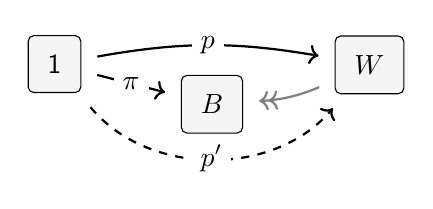
\begin{tikzpicture}[center base]
			% \useasboundingbox (-3,-1) rectangle (3.5,4);
			\node[dpadded] (1) at (0,0.51) {$\sf 1$};
			\node[dpadded] (W) at (4,0.5) {$W$};
			\node[dpadded] (B) at (2,0) {$B$};
			% \node[dpadded] (E) at (6, 0.5 ){$E$};
			% \coordinate (Q) at (6,0); % to even out controls

			\draw[arr] (1) to[bend left=10] node[fill=white]{$p$} (W);
			\draw[arr] (1) to node[fill=white]{$\pi$} (B);

			\draw[arr, gray, ->>] (W) to[bend left=10] (B);
			% \draw[arr, dashed] (B) to[bend right=30] (W);	
			\draw[arr, dashed] (1) to[bend right=50] node[fill=white]{$p'$}(W);	
			% \draw[arr, ->>] (W) to (E);

			% \draw[arr,blue!50] (1) .. controls (2, -1) and (4,-1) .. node[fill=white]{$p'(E)$} (E);
			% \draw[arr,orange!70] (1) .. controls (2,2) and (4,2) .. node[fill=white]{$p(E)$} (E);
		\end{tikzpicture}}
		\caption{PDG Belief Updating via Inconsistency}
		\label{fig:belief-update}
	\end{figure}
}
%joe18: \end{commentout}
	% To understand the update visually in \Cref{fig:belief-update}, imagine the original distribution $p$ from $\sf 1$ to $W$ being replaced by the path $p' := p(W \mid B) \circ \pi$  on the left. The gray arrow on the bottom left is the definition of the random variable, as in \Cref{ex:randomvars}, and the dashed one is its inversion, which can be computed by Bayes' rule.  %that factors through $B$ via the new observation $\pi$.
	% To query the resulting distribution on, an arbitrary event $E$, with an indicator variable of the same name. Initially, we got a marginal on $E$ by going through $p$; we now use $p'$. Effectively, the orange path to $E$ has been replaced by the blue one.
	% 
	% 
	% To observe $\pi$, we simply view it as a cpd conditioned on $\star$ and add it to our collection. 
	% Although it is likely to be inconsistent, resolving this inconsistency in a way that retains $\pi$ is a belief update. 
	% Even failure retain $\pi$ entirely may not be a concern: so long as an they continue to observe or remember, an agent endures discomfort until $\pi$ is incorporated. This setting is arguably more natural than a standard one: without spending energy, it is easy to forget or partially reject implications of the observation.	
	% Once again, with a PDG, the resolution need not happen immediately. This makes the approach more convincing for cognitively bounded agents, who might have more pressing matters than sorting through beliefs, and who might do them out of order.
}%\end{commentout}
\vleftovers{
	\section{Algorithms} 
		\label{sec:algorithms}
	\subsection{Belief Propagation}
	
	
	\subsection{Sampling}
	
	One of the nice about directed graphical models is that the model itself is roughly a sampling algorithm. For instance, taking a Bayes Net $\cal B$ and generating samples according to the tables is an efficient way to sample $\Pr_{\mathcal B}$.

	This works because there is only one path, but more generally, for any conditional marginal $Y|X$, we can think of all of the different paths in the PDG different ways an agent with knowledge $\dg M$ can get probabilistic estimates of the conditional distribution $\bbr{\dg M}\MaxEnt(Y | X)$. The next result states that, in a precise sense, these various estimates bound the location of the marginal for this maximum entropy distribution, which suggests an efficient sampling algorithm for $\bbr{\dg M}\MaxEnt(Y | X)$, after learning some weights.
	
	\begin{conj}\label{thm:maxent-hull}
		For any PDG $\dg M = \pdgvars[]$ containing variables $X, Y$, the maximum entropy conditional marginal $\bbr{\dg M}\MaxEnt(y \mid x)$ is a convex mixture of the conditional marginals generated by the paths from $X$ to $Y$.  That is, there exist weights $\{\alpha_i \geq 0\}$ on the paths in $\dg M$ and a bias weight $\alpha_0$ with $\sum_i {\alpha_i} = 1$ and
		\[ \bbr{\dg M}\MaxEnt(Y \mid X) = \alpha_0 \  p^{\text{unif}}_Y \sum_{p \in \bbr{\dg M}_\lambda(X, Y)} \alpha_i (p_1 \circ \ldots \circ p_k) \]
		where $p^{\text{unif}}_Y$ is the uniform distribution on $Y$, and $\bbr{\dg M}_\lambda(X,Y)$ is the set of paths from $X$ to $Y$ generated by composition and Bayes Rule in $\dg M$. 
	\end{conj}

	One natural choice of these $\alpha$'s is the certainty scores for each edge, given by a weighted PDG, but we do not have any further formal results in this direction.
	Note that it is common for humans to make decisions in this way: to estimate whether something is realistic by following multiple chains of reasoning weighting them by strength of argument.
	
%	\begin{conj}
%		The conditional marginal of the maximum entropy distribution $\bbr{M}\MaxEnt(b \mid a)$ is in the convex hull of the compositions of paths $A \to B$. 
%	\end{conj}
}


	\section{Discussion}
        %oli8: entirely rewritten.
%joe7* It will need to be rewritten again, I'm afraid.  We should hint
%at what PDGs are good for: the fact that we can keep track of
%different, possibly conflict sources of information (we should make a
%bigger deal of that in the intro), the fact that we can capture lots
%of distributions (we hinted at that; can we say more?), the fact that
%they are modular (which lets us put together different sources of
%information) and the fact
%that we can model inconsistency and how people recover from
%inconsisency.  This will require us to get into the dynamics of PDGs
%(how people recover from inconsistency) and will require another
%paper, but we should mention it here.  A good discussion will easily
%fill up the 8th page.
%oli9: I agree, this plan sounds excellent. While you do your pass, I will write a draft of this in a separate document. 
%oli10        
\commentout{
	Given more computation, would your beliefs be more consistent? Or would you explore further, forming more extensive networks of them?
	The canonical picture of an idealized agent has always given the first answer, but this may not necessarily be the case.
}
 
 	% Do dogs have more or less consistent beliefs than we do? 
%oli8
	% They may just not have as many concepts.
	% It may be that they are no less consistent, but just have fewer concetpts.

%oli10: deleted the previous text, 
	% We have given the semantics of PDGs, a modeling framework that enables formal reasoning about this kind of mental state, and is strictly more expressive than the class of Bayesian Networks. The scoring semantics for fixed $\beta_L = \gamma = 1$ recovers the factor graph. The distribution given by a PDG, however is not generally this one, but rather one that is as consistent as possible with the supplied cpds.
	% 
	% The material covered in the present paper is only part of the picture. There are two very important generalizations that we plan to cover next. First, by minorly relaxing the definition of a cpd so that it doesn't need to provide a distribution for a special \texttt{null} value, we gain a huge amount of expressive power, allowing for simpler representations of events and partial knowledge.
 	% Second, while we have discussed what happens in the limit as $\gamma \to 0$, emphasizing the quantitative part of the PDG, there is also a rich story to be told about the qualitative half. Together with the modularity provided by the PDG, and the relaxation to strict PDGs, PDGs are able to function as causal models.
%oli10: new text.
%joe9*: rewrote completely.  You have a few lines to say more.  It
%would also be good to squeeze in somewhere something about related
%work (e.g., perhaps dependency networks).
\commentout{
PDGs are a powerful tool for representing local probabilistic information.
	Though represented by a graph, the edges are interpreted
        differently. Each edge alone determines a cpd, making PDGs
        formally analogous to a commutative diagram, instead of a
        flow-chart. A more familiar network can be obtained with the
        use of multi-tailed arrows. 

	PDGs have a parameterized semantics $[[ - ]]_\gamma$, which always generalizes Bayesian Networks, and precisely becomes a factor graph when $\gamma=1$.  This exposes an implicit trade-off between quantitative and qualitative data; the two behave very differently, but are unfortunately fused in a factor graph. Both qualitative and quantitative information can be inconsistent, although the former is less straightforward, this preliminary paper we focus on the quantitative limit.

	Incorporating new variables, data, or restricting to subgraphs
        of a PDG is simple, making it possible to construct one by
        simply throwing together some pre-trained statistical
        models. Moreover, in the quantitative limit, PDGs continue to
        have local meaning, in stark contrast with energy-based models
        such as factor graphs. As a result, PDGs are not only a
        flexible representation, but modular as well. 

	The most dramatic feature of PDGs is their ability to deal with inconsistency. A PDG can track conflicting information from different sources, and its semantics identify when this occurs, rather than quietly sweeping problems under the rug.
	As a result, a user may resolve inconsistency in multiple ways. Inconsistency can be dealt with by updating one or multiple tables, by introducing introducing or splitting variables, or even left unresolved as as one searches for clarification. The pain of inconsistency can be mitigated by expressing a decreased confidence, without altering any data. 
}
%joe9: \end{commenout}
We have introduced PDGs, a powerful tool for representing
probabilistic information. 
%oli11: trying again to integrate some of what I wrote above in
%clearer terms. Note that now the commutative diagram hint comes in
%the syntax section.
%joe10*  NO!!  Do NOT mention commutative diagrams. It's a distraction.
%It's also not true that PDGs are equivalent to BN's when both are
%rooted trees.  You also need to require that there are no parallel
%edges.  I just cut this sentence
%Although PDGs are visually similar to a BNs and equivalent when both
%are rooted trees, a slight change in the way edges are interpreted
%brings them in line with commutative diagrams, 
%and makes them
%oli11: I like this adjective more than you do; you're welcome to find a new one
%dramatically
%%
%more expressive. 
They have a number of advantages of other
graphical representations:
\begin{itemize}
  \item They allow us to capture inconsistency,
including conflict information from multiple sources, and
%oli11
% confidence about pieces of information.
express variable confidence in the information. 
\item 
They are much more
modular 
%oli11: If modularity = flexibility + ability to break into local components with meaning, then I buy this.
% If modularity = flexibility of adding things, it's only true for directed models; factor graphs are modular as hell but difficult to interpret and only have global meaning.
than other representations; 
for example, we can
combine information from two sources by simply taking the union of two
PDGs, and it is easy to add new information 
%oli11 added
%joe10: cut; I don't undrstand what this means
%(edges, including any statistical model you happen to have)
(edges)
%oli11: I want something simpler than "representational capacity" but
%I can't think of what to say instead 
%joe10: I odn't know what ``representational capacity'' means.
%and representational capacity (nodes)
and features (nodes)
%oli11
% regarding nodes and edges
without affecting previously-received information.
%oli11: I like what you have written, but my paragraph above says a
%lot more. I'm trying to merge them to make it clearer. 
%oli11: This local meaning is super important. It was in the equation,
%but I keep not being able to show it directly; I'll try to re-word.  
%joe10: we haven't even defined restrictions, nor have we explained
%this point.  You can't bring it up out of the blue now!  After
%starting to make changs, I just cut this sentence
%oli12: we have now explained the point. I'm inserting a part of this
%again.
%joe11*: we have *not* empahsized the point.  Nowhere do we talk about
%preserving local meanings of cpds, nor explained why this is important.
%In addition to their flexibility (and unlike similarly flexible models
%such factor graphs), PDGs are unique in also preserving the local
%meanings of their cpds.  
%oli13*: This is an important subtlety --- if by "modular" you mean
% flexiblle, then factor graphs are in some sense better than PDGs (you don't
% even need to normalize your factors!), but we have not time or space. 
% I guess I have to drop it..
\commentout{
%In stark contrast to factor graphs,
In contrast to factor graphs,
%joe10: I don't agree
%oli12*: Why not? You can just add a factor anywhere.
%which are equally flexible,
restrictions of PDGs continue to 
%joe10: you keep using words like ``local'' and ``global''; I don't
%know what they mean.  We can't introduce them out of the blue
retain the same local commitment to the meanings of cpds in the
restriction; this is  
As a result, PDGs exhibit both flexibility and locality, making them
uniquely modular. 
}
\item They allow for a clean separation between quantitiatve
  information (the cpds) and more qualitative information contained by
%joe10
%  the graph struture; this is captured by the terms $\Inc$ and $\IDef$
    the graph structure; this is captured by the terms $\Inc$ and $\IDef{}$
  in our scoring function.
\item PDGs have (several) natural semantics;
%oli11 added
%joe10: I don't understand this
  %, each of which paints a global probabilistic picture with
  %  constraints,
%oli12: this was clarified in the semantics introduction now. edited
%and reinstated. 
%joe11: this was *not* clarified in the introduction, and I don't like
%the terminology.  What does it mean to bear on 
%  each of which which bears on global properties of joint distributions,
%  making a PDG more useful than a mere collection of data. 
one of them (under some assumptions) allows us to pick out a unique
distribtuion specified by the PDG.   This, in turn, shows that PDGS 
%joe11: combined
%
%\end{itemize}
%We showed that PDGs
can capture BNs and factor graphs, in the latter case by choosing 
appropriate parameters in the scoring rule. However, they also avoid
%joe10*: let's make sure that we do this
some of the arguably unnatural properties of factor graphs (a point
discussed in more detail in the appendix).
%joe11
\end{itemize}

We have only scratched the surface of what can be done with PDGs here.
%oli11:added
%joe10: this sentence tailed off.  Feel free to add it again
%For simplicitly of presentation, we have only allowed PDGs to express 
%
One issue we hope to foucs on in the future is dynamics.  We believe
that PDGs will prove a particularly useful tool for examining how agents resolve
inconsistency%
%oli11: inefficient use of space
% , moving from an inconsistent state to a consistent state.
.
%oli11: added
%joe10: This is not ``Moreover''.  It's not quite the right story
%Moreover, it seems that the setups to a very large class of standard
%naturally encoded as PDGs, while their standard resolutions (resp.,
%naturally encoded as PDGs; the standard approaches to deal
%with them (resp.,
%variational inference, Bayesian updating) can be regarded as
%reductions of its inconsistency.   
Inconsistency resolution is a pervasive phenomenon.
For example, belief updating can be naturally viewed as an instance of
resolving inconsistency: We now believe that something is true to
which we earlier assigned probabiity less than 1.  Conditioning can be
viewed as a way of resolving that inconsistency (as can other more
general approaches to belief updating, such as Jeffrey's Rule
\cite{Jeffrey68}. 
%joe10: I don't understand how variational inference fits in, but if
%you can write a clear, crisp sentence, we can add it.
%probability less than 
%problems (e.g., variational approximation, belief updating) are
%
This makes representing inconsistent information using a PDG and then
resolving it an topic that can have a potentially high payoff.
We hope to report on this in the future.

	% \subsection{Probabilities Still Encode Well}	
	% In some sense, while we have yet to find a mental state that
	% is not encoded in some probability distribution, the choice
	% of underlying space is extremely important, and we argue
	% that it changes rapidly. Moreover, sometimes one has to make
	% up new internal mental variables, which also changes the
	% underlying space. PDGs offer a way to describe
	% distributions, together with a number of internal parameters
	% one might not be actively aware of. The relevant parameters,
	% can always be internalized \todo{define internalization}
	% until we reach a distribution.  
	% 
	% However, storing knowledge in the form of another graphical model is extremely cumbersome if the set of worlds changes quickly.	
	% 
	% \begin{example}
	% 	\todo{recall coin example, internalize biases, sets of dists, etc.}
	% \end{example}
	% \begin{example}
	% 	\todo{Point to appendix where we discuss factor graph conversions: these internalize the energy}
	% \end{example}

%joe17* this does not belong in a paper on PDGs
\vfull{
		\subsection{Inconsistency} \label{sec:consistency-ethos}
	
		Believing a logically inconsistent formula can lead you to arbitrarily bad conclusions, having an infeasible set of constraints makes all answers you could give wrong, and having inconsistent preferences can lose you infinite money. We don't want to build inconsistent systems or agents with incoherent views of the world, and so, where possible, we design them so they cannot possibly be broken in this way. Suppose, for example, that we are trying to represent some quantity that must be a point on the unit circle. We could do it with an $x$ and $y$ coordinate, but this could be problematic because $x^2+ y^2$ might not be 1 --- it would be safer and harder to go awry if we parameterize it by an angle $\theta \in [0, 2\pi)$ instead. In the absence of performance benefits (like needing to regularly use the $y$-coordinate and not wanting to compute a sine), why would we take the first approach, introducing a potentially complex data-invariant, when we could avoid it?
		
		This line of thought, though common and defensible, is flawed if we are not perfectly confident in the design of both our system and the ways it can interact with the outside world. Using similar logic, we might ask ourselves: Why ask programmers for type annotations when all instructions are operationally well-defined at run-time?  Why use extra training data if there's already enough there to specify a function? Why estimate a quantity in two ways when they will yield different answers? Why repeat and rephrase your ideas when this could make you contradict yourself? Why write test cases when they could fail and make the project inconsistent? Why conduct an experiment if it could just end up contradicting your current knowledge?
		
		These questions may seem silly, but there is a satisfying information theoretic answer to all of them: redundancy, though costly, is the primary tool that we use to combat the possibility of being wrong. Maintaining data invariants can be expensive but provides diagnostic information; in the example above, settings of $x$ and $y$ that don't lie on the unit circle provide diagnostic information that something has gone wrong.
		In many cases, it is also possible to paper over problems by forcibly re-instating local data invariants: for instance, we could re-normalize any values of $x$ and $y$ (so long as $xy \neq 0$; we can chose an arbitrary point otherwise) at every step. While this would reduce inconsistency, it also hides red flags.
		
		Using a Bayesian Network to represent a probability distribution is like representing a circle with $\theta \in [0, 2\pi)$.
		By construction, the result must be a distribution, and nothing can possibly go wrong so long as we can always decide on exactly one distribution which is sufficient for our purposes.
		%	By construction, the result must be a point on the circle, and nothing can possibly go wrong so long as we're sure that we will always have exactly enough information to determine such a point (for instance, we could never be totally clueless about the point, or just know its $x$ coordinate).
		
		
		The process of mechanistically forcing invariants is homologous to the standard practice for factor graphs: practitioners will often just assume that the density it defines is normalizable, and either forcibly re-normalize or cleverly avoid computing the normalization constant while still assuming that one exists; behavior is usually left unspecified in the unlikely event that it is not defined or zero.
%joe17
}
	
	
%oli8: removing
	% \section{Conclusions}
	
	% \subsection{A LIST OF PDG BENEFITS}\label{sec:list-of-benefits}
	% \todo{Remove and refactor into appendix}
	% \begin{enumerate}[nosep]
	% 	\item PDGs can represent both over-constrained and under-constrained mental states. 
	% 	\item In particular, they may be inconsistent, which gives agents using PDGs the qualitatively new kind of `epistemic modesty': the possibility of realizing that something is wrong with their beliefs.
	% 	\item Many standard algorithms, including as belief propogation, conditioning, and belief revision, can be regarded as resolution of inconsistency.
	% 	\item PDGs can emulate the functionality of other graphical graphical models.
	% 	\item PDGs are more modular, making it much less invasive to combine, reduce, or partially interpret parts of the model, compared to alternatives.
	% 	\item The modularity enables type-forming rules which can be used to implement deductive inference.
	% 	\item The many standard ways of adding and eliminating variables provides an answer to the question, ``why these possible worlds?''
	% 	\item Compared with a standard constraint satisfaction problem, individual components have of have limited impact on the semantics.
	% 	\item The class of free energies defined by PDGs is strictly more expressive than those given by alternative graphical models.
	% \end{enumerate} % trade-off: harder to analyze.
	

\clearpage

%joe17: I didn't check with AAAI wanted in their ethics statement.
%I'm not sure we really need this.
%oli20: It's optional. But it doesn't use paper space, we have something interesting to say, and already have a draft.
	\section*{Ethics Statement}
	% Authors are required to include a statement of the broader impact of their work, including its ethical
	% aspects and future societal consequences. Authors should discuss both positive and negative outcomes,
	% if any. For instance, authors should discuss a) who may benefit from this research, b) who may be
	% put at disadvantage from this research, c) what are the consequences of failure of the system, and d)
	% whether the task/method leverages biases in the data. If authors believe this is not applicable to them,
	% authors can simply state this
%joe10*: rewrote
Because PDGs are a recent theoretical development, there is a lot of
guesswork in evaluating the impact. Here are two views of
%joe1
%opposit polarities.
opposite polarity.

\subsection{Positive Impacts}
One can imagine many applications of enabling simple and coherent
aggregation of (possibly inconsistent) information. In particular we
can imagine using PDGs to build and interpret a communal and global
database of statistical models, in a way that may not only enable more
accurate predictions, but also highlights conflicts between
information.

%joe1: what does fairness have to do with any of the above or below?
%This could have a critical impact on the state of fairness.
This could have many benefits.
Suppose, for instance, that two researchers train models, but use
datasets with
different racial makeups. Rather than trying to get an uninterpretable
%joe1
%model to "get it right" the first time, we could simply highlight any
model to ``get it right'' the first time, we could simply highlight any
%joe1
%such clashes and flag them for review---without needing to see
%feedback from the rest of the world.
such clashes and flag them for review.

%joe1: this seems redundant, so I cut it
%It is well-known that the statistically optimal prediction will
%generally not be well-calibrated and fair. 
Rather than trying to
ensure fairness by design which is both tricky and costly,
we envision an alternative: simply use
statistically optimal results, while allowing socail systems to resolve conflicts,
rather than fiddling with loss functions ourselves.
%joe7: \end{commentout}
% \end{notfocus}

\subsection{Negative Impacts}

We can also imagine less rosy outcomes. To the extent that PDGs can
model and reason with inconsistency,
%joe1: I didn't really undesrtand what you wrote below, so I cut it.
%one might worry that PDGs will
%reproduce some of the ``less rational'' human behavior. Because PDGs
%make it so easy to add information without computation, one can
%imagine a naive implementation being particularly vulnerable to
%attacks where it is fed more data than it can reasonably process. As
if
we adopt the attitude that a PDG need not wait until it is consistent
%joe1
%for use, it is not hard to see a world where it gives very biased and
%poorly-thought out conclusions---such a PDG might be likened to a
%conspiracy theorist, constantly absorbing too much information to
%process it correctly.
to be used, it is not hard to imagine a world where a PDG gives biased and
poorly-thought out conclusions.
It is clear that PDGs need a great deal more
vetting before they can be used for such important purposes as
aggregating the world's statistical knowledge.

PDGs are powerful statistical models, but are by necessity
semantically more complicated than many existing methods. This will
likely restrict their accessibility. To mitigate this, we commit to
making sure our work is widely accessible to researchers of different
backgrounds.



{
    % \small
    % \bibliographystyle{alpha}
    \bibliography{allrefs,z,joe}        
}
%\addbibresource{../uncertainty.bib}
%\addbibresource{../maths.bib}
%\addbibresource{graphical-models.bib}

\appendix
\clearpage
\onecolumn
%
\def\year{2021}\relax
% File: formatting-instruction.tex

\documentclass[letterpaper]{article} % DO NOT CHANGE THIS
\usepackage[margin=1in]{geometry}
% \usepackage{aaai21} % DO NOT CHANGE THIS
\usepackage{times} % DO NOT CHANGE THIS
\usepackage{helvet} % DO NOT CHANGE THIS
\usepackage{courier} % DO NOT CHANGE THIS
\usepackage[hyphens]{url} % DO NOT CHANGE THIS
\usepackage{graphicx} % DO NOT CHANGE THIS
\urlstyle{rm} % DO NOT CHANGE THIS
\def\UrlFont{\rm} % DO NOT CHANGE THIS
\usepackage{graphicx} % DO NOT CHANGE THIS
\usepackage{natbib} % DO NOT CHANGE THIS OR ADD OPTIONS
\usepackage{caption} % DO NOT CHANGE THIS OR ADD OPTIONS
\frenchspacing % DO NOT CHANGE THIS
\setlength{\pdfpagewidth}{8.5in} % DO NOT CHANGE THIS
\setlength{\pdfpageheight}{11in} % DO NOT CHANGE THIS

\usepackage{tikz}
	\usetikzlibrary{positioning,fit,calc, decorations, arrows, shapes, shapes.geometric}
	\usetikzlibrary{backgrounds}
	\usetikzlibrary{patterns}
	\usetikzlibrary{cd}
	
	\pgfdeclaredecoration{arrows}{draw}{
		\state{draw}[width=\pgfdecoratedinputsegmentlength]{%
			\path [every arrow subpath/.try] \pgfextra{%
				\pgfpathmoveto{\pgfpointdecoratedinputsegmentfirst}%
				\pgfpathlineto{\pgfpointdecoratedinputsegmentlast}%
			};
	}}
	%%%%%%%%%%%%
	\tikzset{AmpRep/.style={ampersand replacement=\&}}
	\tikzset{center base/.style={baseline={([yshift=-.8ex]current bounding box.center)}}}
	\tikzset{paperfig/.style={center base,scale=0.9, every node/.style={transform shape}}}

	\tikzset{is bn/.style={background rectangle/.style={fill=blue!35,opacity=0.3, rounded corners=5},show background rectangle}}
	% Node Stylings
	\tikzset{dpadded/.style={rounded corners=2, inner sep=0.7em, draw, outer sep=0.3em, fill={black!50}, fill opacity=0.08, text opacity=1}}
	\tikzset{dpad0/.style={outer sep=0.05em, inner sep=0.3em, draw=gray!75, rounded corners=4, fill=black!08, fill opacity=1}}
	\tikzset{dpad/.style args={#1}{every matrix/.append style={nodes={dpadded, #1}}}}
	\tikzset{light pad/.style={outer sep=0.2em, inner sep=0.5em, draw=gray!50}}
		
	\tikzset{arr/.style={draw, ->, thick, shorten <=3pt, shorten >=3pt}}
	\tikzset{arr0/.style={draw, ->, thick, shorten <=0pt, shorten >=0pt}}
	\tikzset{arr1/.style={draw, ->, thick, shorten <=1pt, shorten >=1pt}}
	\tikzset{arr2/.style={draw, ->, thick, shorten <=2pt, shorten >=2pt}}
	\tikzset{archain/.style args={#1}{arr, every arrow subpath/.style={draw,arr, #1}, decoration=arrows, decorate}}


	\tikzset{fgnode/.style={dpadded,inner sep=0.6em, circle},
	factor/.style={light pad, fill=black}}	
	
	
	\newcommand\cmergearr[4]{
		\draw[arr,-] (#1) -- (#4) -- (#2);
		\draw[arr, shorten <=0] (#4) -- (#3);
	}
	\newcommand\mergearr[3]{
		\coordinate (center-#1#2#3) at (barycentric cs:#1=1,#2=1,#3=1.2);
		\cmergearr{#1}{#2}{#3}{center-#1#2#3}
	}
	\newcommand\cunmergearr[4]{
		\draw[arr,-, , shorten >=0] (#1) -- (#4);
		\draw[arr, shorten <=0] (#4) -- (#2);
		\draw[arr, shorten <=0] (#4) -- (#3);
	}
	\newcommand\unmergearr[3]{
		\coordinate (center-#1#2#3) at (barycentric cs:#1=1.2,#2=1,#3=1);
		\cunmergearr{#1}{#2}{#3}{center-#1#2#3}
	}

	
	\usetikzlibrary{matrix}
	\tikzset{toprule/.style={%
	        execute at end cell={%
	            \draw [line cap=rect,#1] 
	            (\tikzmatrixname-\the\pgfmatrixcurrentrow-\the\pgfmatrixcurrentcolumn.north west) -- (\tikzmatrixname-\the\pgfmatrixcurrentrow-\the\pgfmatrixcurrentcolumn.north east);%
	        }
	    },
	    bottomrule/.style={%
	        execute at end cell={%
	            \draw [line cap=rect,#1] (\tikzmatrixname-\the\pgfmatrixcurrentrow-\the\pgfmatrixcurrentcolumn.south west) -- (\tikzmatrixname-\the\pgfmatrixcurrentrow-\the\pgfmatrixcurrentcolumn.south east);%
	        }
	    },
	    leftrule/.style={%
	        execute at end cell={%
	            \draw [line cap=rect,#1] (\tikzmatrixname-\the\pgfmatrixcurrentrow-\the\pgfmatrixcurrentcolumn.north west) -- (\tikzmatrixname-\the\pgfmatrixcurrentrow-\the\pgfmatrixcurrentcolumn.south west);%
	        }
	    },
	    rightrule/.style={%
	        execute at end cell={%
	            \draw [line cap=rect,#1] (\tikzmatrixname-\the\pgfmatrixcurrentrow-\the\pgfmatrixcurrentcolumn.north east) -- (\tikzmatrixname-\the\pgfmatrixcurrentrow-\the\pgfmatrixcurrentcolumn.south east);%
	        }
	    },
	    table with head/.style={
		    matrix of nodes,
		    row sep=-\pgflinewidth,
		    column sep=-\pgflinewidth,
		    nodes={rectangle,minimum width=2.5em, outer sep=0pt},
		    row 1/.style={toprule=thick, bottomrule},
  	    }
	}
\newif\ifprecompiledfigs
\precompiledfigsfalse
% \precompiledfigstrue

\newif\ifexternalizefigures\externalizefiguresfalse

\newif\ifappendix\appendixtrue
\newif\ifbody\bodyfalse

\ifexternalizefigures\else
	\usetikzlibrary{external}
	\tikzexternalize[prefix=tikz/]  % activate!
	% \usepackage{etoolbox}
	%  \AtBeginEnvironment{tikzcd}{\tikzexternaldisable} %... except careful of tikzcd...
	%  \AtEndEnvironment{tikzcd}{\tikzexternalenable}
\fi
%END_FOLD


%BEGIN_FOLD: Theorems and Tools

\usepackage{booktabs}       % professional-quality tables
\usepackage{amsfonts}       % blackboard math symbols
\usepackage{nicefrac}       % compact symbols for 1/2, etc.
\usepackage{microtype}      % microtypography
\usepackage{mathtools}		%also loads amsmath
\usepackage{amssymb, bbm}

%oli20: oops, this is vorboten :(
% \usepackage[format=plain,
%             labelfont={sl},
%             textfont={it,small}]{caption}

\usepackage{relsize}
\usepackage{environ} % http://ctan.org/pkg/environ; for capturing body as a parameter for idxmats

\usepackage{color}
%\usepackage{stmaryrd}

\usepackage{amsthm}
\usepackage{thmtools}

\theoremstyle{plain}
\newtheorem{theorem}{Theorem}[section]
\newtheorem{coro}{Corollary}[theorem]
\newtheorem{prop}[theorem]{Proposition}
\newtheorem{lemma}[theorem]{Lemma}
\newtheorem{fact}[theorem]{Fact}
\newtheorem{conj}[theorem]{Conjecture}

\theoremstyle{definition}

% no section numbers for theorems in AAAI style ... 
%joe17: can you reinstate this?
%oli20:done
\declaretheorem[name=Definition,qed=$\square$,numberwithin=section]{defn} %
\declaretheorem[name=Construction,qed=$\square$,sibling=defn]{constr}
\declaretheorem[qed=$\square$]{example}

\theoremstyle{remark}
\newtheorem*{remark}{Remark}

\usepackage{xstring}
\usepackage{enumitem}

\usepackage{environ}
\usepackage{xstring}

% Wow this works I'm brilliant
\def\wrapwith#1[#2;#3]{
	\expandarg\IfSubStr{#1}{,}{
		\expandafter#2{\expandarg\StrBefore{#1}{,}}
		\expandarg\StrBehind{#1}{,}[\tmp]
		\xdef\tmp{\expandafter\unexpanded\expandafter{\tmp}}
		#3
		\wrapwith{\tmp}[#2;{#3}]
	}{ \expandafter#2{#1} }
}
\def\hwrapcells#1[#2]{\wrapwith#1[#2;&]}
\def\vwrapcells#1[#2]{\wrapwith#1[#2;\\]}
\NewEnviron{mymathenv}{$\BODY$}

\newcommand{\smalltext}[1]{\text{\footnotesize#1}}
\newsavebox{\idxmatsavebox}
\def\makeinvisibleidxstyle#1#2{\phantom{\hbox{#1#2}}}
\newenvironment{idxmatphant}[4][\color{gray}\smalltext]{%
	\def\idxstyle{#1}
	\def\colitems{#3}
	\def\rowitems{#2}
	\def\phantitems{#4}
	\begin{lrbox}{\idxmatsavebox}$%$\begin{mymathenv}
	\begin{matrix}  \begin{matrix} \hwrapcells{\colitems}[\idxstyle]  \end{matrix}
		% &\vphantom{\idxstyle\colitems}
		\\[-0.05em]
		\left[
		\begin{matrix}
			\hwrapcells{\phantitems}[\expandafter\makeinvisibleidxstyle\idxstyle]  \\[-1.2em]
	}{
		\end{matrix}\right]		&\hspace{-0.8em}\begin{matrix*}[l] \vwrapcells{\rowitems}[\idxstyle] \end{matrix*}\hspace{0.1em}%
	\end{matrix}%
	$%\end{mymathenv}
	\end{lrbox}%
	\raisebox{0.75em}{\usebox\idxmatsavebox}
%	\vspace{-0.5em}
}

\newenvironment{idxmat}[3][\color{gray}\smalltext]
	{\begingroup\idxmatphant[#1]{#2}{#3}{#3}}
	{\endidxmatphant\endgroup}

\newenvironment{sqidxmat}[2][\color{gray}\smalltext]
	{\begingroup\idxmat[#1]{#2}{#2}}
	{\endidxmat\endgroup}


%%%%%%%%%%%%
% better alignment for cases
\makeatletter
\renewenvironment{cases}[1][l]{\matrix@check\cases\env@cases{#1}}{\endarray\right.}
\def\env@cases#1{%
	\let\@ifnextchar\new@ifnextchar
	\left\lbrace\def\arraystretch{1.2}%
	\array{@{}#1@{\quad}l@{}}}
\makeatother

\newcommand\numberthis{\addtocounter{equation}{1}\tag{\theequation}}

%oli20: apparently this is not allowed in AAAI style.
%oli21: but it helps me edit so I'm reenabling it until later
%oli25:
% \usepackage{xr}
% \usepackage{xr-hyper}
\usepackage{zref-xr}
% \usepackage{hyperref}
\zxrsetup{toltxlabel=true, tozreflabel=false}
\zexternaldocument*{pdg}
%oli24: the time has come... goodbye links and colors :(
% \usepackage{hyperref}
% \definecolor{deepgreen}{rgb}{0,0.5,0}
% \hypersetup{colorlinks=true, linkcolor=blue!50!black, urlcolor=magenta, citecolor=deepgreen}

\usepackage[noabbrev,nameinlink,capitalize]{cleveref}
\crefname{example}{Example}{Examples}
\crefname{defn}{Definition}{Definitions}
\crefname{prop}{Proposition}{Propositions}
\crefname{constr}{Construction}{Constructions}
\crefname{conj}{Conjecture}{Conjectures}
\crefname{fact}{Fact}{Facts}
%\crefname{section}{\S\!}{\S\!}


\usepackage{float}
% \usepackage{subcaption}
\newcounter{subfigure}
	% \captionsetup[subfigure]{subrefformat=simple,labelformat=simple}
	\renewcommand\thesubfigure{\thefigure(\alph{subfigure})}
    
\newenvironment{old}[1]{\par\noindent{\bf \Cref{#1}.} \em \noindent}{\par\medskip}

%% Version of recall that pulls the savebox:
% \usepackage{xpatch}
% \makeatletter
% \xpatchcmd{\thmt@restatable}% Edit \thmt@restatable
%    {\csname #2\@xa\endcsname\ifx\@nx#1\@nx\else[{#1}]\fi}% Replace this code
%    % {\ifthmt@thisistheone\csname #2\@xa\endcsname\typeout{oiii[#1;#2\@xa;#3;\csname thmt@stored@#3\endcsname]}\ifx\@nx#1\@nx\else[#1]\fi\else\csname #2\@xa\endcsname\fi}% with this code
%    {\ifthmt@thisistheone\csname #2\@xa\endcsname\ifx\@nx#1\@nx\else[{#1}]\fi
%    \else\fi}
%    {\typeout{oii Success1?}}{\typeout{oiii failure1?}} % execute code for success/failure instances
% \xpatchcmd{\thmt@restatable}% Edit \thmt@restatable
%    {\csname end#2\endcsname}
%    {\ifthmt@thisistheone\csname end#2\endcsname\else\fi}
%    {\typeout{oii Success2?}}{\typeout{oiii failure2?}}
% \newcommand{\recall}[1]{\medskip\par\noindent{\bf \expandarg\Cref{thmt@@#1}.} \begingroup\em \noindent
%    \expandafter\csname#1\endcsname* \endgroup\par\smallskip}
% \makeatother

\newcommand{\restate}[2]
	{\medskip\par\noindent{\bf \expandarg\Cref{thmt@@#1}.}%
 	\noindent\begingroup\em #2 \endgroup\par\smallskip}


%oli16: The extra space was because there was extra space in the paragraph, not
%because this length was too big. By breaking arrays, everything will be better.
\allowdisplaybreaks

\newcommand{\begthm}[3][]{\begin{#2}[{name=#1},restate=#3,label=#3]}

%TODO
\newcommand{\createversion}[2][{gray}{0.75}]{
	\definecolor{v#2color}#1\relax
    \expandafter\xdef\csname v#2on\endcsname{%
		% \xdef\gamma{\tau}%
		% \expandafter\renewcommand\csname v#2\endcsname{ONN}%
		% \expandafter\xdef{\csname v#2on\endcsname}##{{\color{v##2color} #1}}
	}
	\expandafter\xdef\csname v#2off\endcsname{
	% 	\expandafter\newcommand\csname v #2\endcsname[1]{{\color{v ##2 color} #1}}
	}
}
\createversion{test}
% \vteston
%END_FOLD

%BEGIN_FOLD   %%%% Version knobs %%%%%. 
%oli20: your commenting system is better than the one based on comment package, 
% which is way more problematic than I thought.
% I'm killing it and refactoring all comments to be like yours. I'm not annotating
% everything I'm doing here but the result will be way clearer and less problematic.

\definecolor{vfullcolor}{gray}{0.7}
\newcommand\vfull[1]{{\color{vfullcolor} #1}}
\renewcommand\vfull[1]{} % disable vfull

\definecolor{vleftoverscolor}{gray}{0.85}
\newcommand{\vleftovers}[1]{{\color{vleftoverscolor} #1}} 
\renewcommand{\vleftovers}[1]{} %disable vleftovers

\definecolor{notationcolor}{rgb}{0.9,0.9,.9} 
\newcommand{\notation}[1]{{\color{notationcolor} #1}}
\renewcommand{\notation}[1]{\ignorespaces} % disable notation

\definecolor{contentiouscolor}{rgb}{0.7,0.3,.1} 
\newcommand{\commentout}[1]{\ignorespaces} 

% \newcommand{\contentious}[1]{
% 	\noindent\colorbox{red!10!white}{\parbox{\linewidth-3pt}{\color{red!10!black}#1}}}
% \newcommand{\valpha}[1]{%
% 	% \colorbox{red!10!white}
% 	{\color{red!10!black}{#1}}%
% }
% \newcommand{\valpha}[1]{{\color{red!80!black}#1}}
\newcommand{\valpha}[1]{#1}

%END_FOLD


%BEGIN_FOLD definitions
%BEGIN_FOLD %%%%%   general shorthand I use   %%%%%%%%%%%%%%%%%

%\usepackage{stmaryrd}
%\DeclarePairedDelimiter{\ccbr}{\lBrace}{\rBrace}
%\DeclarePairedDelimiter{\bbr}{\llbracket}{\rrbracket}
%\DeclarePairedDelimiter{\ppr}{\llparenthesis}{\rrparenthesis}

\DeclarePairedDelimiterX{\bbr}[1]{[}{]}{\mspace{-3.5mu}\delimsize[#1\delimsize]\mspace{-3.5mu}}
\DeclarePairedDelimiter{\norm}{\lVert}{\rVert}

\let\Horig\H
\let\H\relax
\DeclareMathOperator{\H}{\mathrm{H}} % Entropy
\DeclareMathOperator{\I}{\mathrm{I}} % Information
\DeclareMathOperator*{\Ex}{\mathbb{E}} % Expectation
\DeclareMathOperator*{\argmin}{arg\;min}
\newcommand{\CI}{\mathrel{\perp\mspace{-10mu}\perp}} % Conditional Independence
\newcommand\mat[1]{\mathbf{#1}}
\DeclarePairedDelimiterX{\infdivx}[2]{(}{)}{%
	#1\;\delimsize\|\;#2%
}
\newcommand{\thickD}{I\mkern-8muD}
\newcommand{\kldiv}{\thickD\infdivx}


\newcommand{\todo}[1]{{\color{red}\ \!\Large\smash{\textbf{[}}{\normalsize\textsc{todo:} #1}\ \!\smash{\textbf{]}}}}
\newcommand{\note}[1]{{\color{blue}\ \!\Large\smash{\textbf{[}}{\normalsize\textsc{note:} #1}\ \!\smash{\textbf{]}}}}



% SPACES
\newcommand\Set{\mathbb{S}\mathrm{et}}
\newcommand\FinSet{\mathbb{F}\mathrm{in}\mathrm{S}\mathrm{et}}
\newcommand\Meas{\mathbb{M}\mathrm{eas}}
\newcommand\two{\mathbbm 2}

%END_FOLD

%BEGIN_FOLD %%%%%    PDG-specific macros     %%%%%%%%%%%%%%%%
\DeclarePairedDelimiterXPP{\SD}[1]{}{[}{]}{_{\text{sd}}}{\mspace{-3.5mu}\delimsize[#1\delimsize]\mspace{-3.5mu}}
		
%\usepackage{stmaryrd}
%\newcommand{\none}{\varobslash}
\newcommand{\none}{\bullet}

\def\sheq{\!=\!}
\DeclareMathOperator\dcap{\mathop{\dot\cap}}
\newcommand{\tto}{\rightarrow\mathrel{\mspace{-15mu}}\rightarrow}

\newcommand{\bp}[1][L]{\mat{p}_{\!_{#1}\!}}
\newcommand{\V}{\mathcal V}
\newcommand{\N}{\mathcal N}
\newcommand{\Ed}{\mathcal E}
\newcommand{\pdgvars}[1][]{(\N#1, \Ed#1, \V#1, \mat p#1, \beta#1)}


\DeclareMathAlphabet{\mathdcal}{U}{dutchcal}{m}{n}
\DeclareMathAlphabet{\mathbdcal}{U}{dutchcal}{b}{n}
%joe1:out of curiousity, why not use \mathcal?  That's what you use
%for BNs.  Why do PDG use a different font?
\newcommand{\dg}[1]{\mathbdcal{#1}}
\newcommand{\var}[1]{\mathsf{#1}}
\newcommand\Pa{\mathbf{Pa}}

%oli20: better spacing
% \newcommand{\IDef}[1]{\mathit{IDef}_{#1}}
\newcommand{\IDef}[1]{\mathit{IDef}_{\!#1}}

\newcommand\Inc{\mathit{Inc}}
\newcommand{\PDGof}[1]{{\dg M}_{#1}}
%oli22: a macro for unweighted PDGs
\newcommand{\UPDGof}[1]{{\dg N}_{#1}}
\newcommand{\WFGof}[1]{\Psi_{{#1}}}
%oli22: and for unweighted ones
\newcommand{\FGof}[1]{\Phi_{{#1}}}
%oli22: want to refer to the variable graph
\newcommand{\Gr}{\mathcal G}
%oli22: Gibbs Free Energy conflicts with \mathcal G. Now it lives in 
% this macro.
\newcommand\GFE{\mathit{G\mkern-4mu F\mkern-4.5mu E}}
%oli22: Right now we're using (\N, \V) to refer to variables of a
% PDG. I think it's important to keep both \N and \V but am happy to change
% the way we combine them. Factored into a macro so it's easier to change.
\newcommand{\varsNV}[1][\N,\V]{(#1)}


% \makeatletter %Arguments: L, X, Y, \scriptscriptstyle, -1pt (for raisebox)
% \newcommand{\ed@helper}[5]{#2\!%
%   \overset{\smash{\mskip-5mu\raisebox{-1pt}{$\scriptscriptstyle
%         #1$}}}{\rightarrow}\! #3} 
% \makeatother

%oli22: the edge notation is now uniform. Choose between the following
% Default: display as "X -L-> Y" (leave uncommented).
\newcommand{\ed}[3]{#2\!%
  \overset{\smash{\mskip-5mu\raisebox{-1pt}{$\scriptscriptstyle
        #1$}}}{\rightarrow}\! #3} 
% Option: uncomment to display as  "L = (X,Y,\ell)" instead.
% \renewcommand{\ed}[3]{#2 = (#1,#3,\ell)} 
\newcommand{\alle}[1][L]{_{ \ed {#1}XY}}


\begin{document}
\appendix
\onecolumn
%
\def\year{2021}\relax
% File: formatting-instruction.tex

\documentclass[letterpaper]{article} % DO NOT CHANGE THIS
\usepackage[margin=1in]{geometry}
% \usepackage{aaai21} % DO NOT CHANGE THIS
\usepackage{times} % DO NOT CHANGE THIS
\usepackage{helvet} % DO NOT CHANGE THIS
\usepackage{courier} % DO NOT CHANGE THIS
\usepackage[hyphens]{url} % DO NOT CHANGE THIS
\usepackage{graphicx} % DO NOT CHANGE THIS
\urlstyle{rm} % DO NOT CHANGE THIS
\def\UrlFont{\rm} % DO NOT CHANGE THIS
\usepackage{graphicx} % DO NOT CHANGE THIS
\usepackage{natbib} % DO NOT CHANGE THIS OR ADD OPTIONS
\usepackage{caption} % DO NOT CHANGE THIS OR ADD OPTIONS
\frenchspacing % DO NOT CHANGE THIS
\setlength{\pdfpagewidth}{8.5in} % DO NOT CHANGE THIS
\setlength{\pdfpageheight}{11in} % DO NOT CHANGE THIS

\usepackage{tikz}
	\usetikzlibrary{positioning,fit,calc, decorations, arrows, shapes, shapes.geometric}
	\usetikzlibrary{backgrounds}
	\usetikzlibrary{patterns}
	\usetikzlibrary{cd}
	
	\pgfdeclaredecoration{arrows}{draw}{
		\state{draw}[width=\pgfdecoratedinputsegmentlength]{%
			\path [every arrow subpath/.try] \pgfextra{%
				\pgfpathmoveto{\pgfpointdecoratedinputsegmentfirst}%
				\pgfpathlineto{\pgfpointdecoratedinputsegmentlast}%
			};
	}}
	%%%%%%%%%%%%
	\tikzset{AmpRep/.style={ampersand replacement=\&}}
	\tikzset{center base/.style={baseline={([yshift=-.8ex]current bounding box.center)}}}
	\tikzset{paperfig/.style={center base,scale=0.9, every node/.style={transform shape}}}

	\tikzset{is bn/.style={background rectangle/.style={fill=blue!35,opacity=0.3, rounded corners=5},show background rectangle}}
	% Node Stylings
	\tikzset{dpadded/.style={rounded corners=2, inner sep=0.7em, draw, outer sep=0.3em, fill={black!50}, fill opacity=0.08, text opacity=1}}
	\tikzset{dpad0/.style={outer sep=0.05em, inner sep=0.3em, draw=gray!75, rounded corners=4, fill=black!08, fill opacity=1}}
	\tikzset{dpad/.style args={#1}{every matrix/.append style={nodes={dpadded, #1}}}}
	\tikzset{light pad/.style={outer sep=0.2em, inner sep=0.5em, draw=gray!50}}
		
	\tikzset{arr/.style={draw, ->, thick, shorten <=3pt, shorten >=3pt}}
	\tikzset{arr0/.style={draw, ->, thick, shorten <=0pt, shorten >=0pt}}
	\tikzset{arr1/.style={draw, ->, thick, shorten <=1pt, shorten >=1pt}}
	\tikzset{arr2/.style={draw, ->, thick, shorten <=2pt, shorten >=2pt}}
	\tikzset{archain/.style args={#1}{arr, every arrow subpath/.style={draw,arr, #1}, decoration=arrows, decorate}}


	\tikzset{fgnode/.style={dpadded,inner sep=0.6em, circle},
	factor/.style={light pad, fill=black}}	
	
	
	\newcommand\cmergearr[4]{
		\draw[arr,-] (#1) -- (#4) -- (#2);
		\draw[arr, shorten <=0] (#4) -- (#3);
	}
	\newcommand\mergearr[3]{
		\coordinate (center-#1#2#3) at (barycentric cs:#1=1,#2=1,#3=1.2);
		\cmergearr{#1}{#2}{#3}{center-#1#2#3}
	}
	\newcommand\cunmergearr[4]{
		\draw[arr,-, , shorten >=0] (#1) -- (#4);
		\draw[arr, shorten <=0] (#4) -- (#2);
		\draw[arr, shorten <=0] (#4) -- (#3);
	}
	\newcommand\unmergearr[3]{
		\coordinate (center-#1#2#3) at (barycentric cs:#1=1.2,#2=1,#3=1);
		\cunmergearr{#1}{#2}{#3}{center-#1#2#3}
	}

	
	\usetikzlibrary{matrix}
	\tikzset{toprule/.style={%
	        execute at end cell={%
	            \draw [line cap=rect,#1] 
	            (\tikzmatrixname-\the\pgfmatrixcurrentrow-\the\pgfmatrixcurrentcolumn.north west) -- (\tikzmatrixname-\the\pgfmatrixcurrentrow-\the\pgfmatrixcurrentcolumn.north east);%
	        }
	    },
	    bottomrule/.style={%
	        execute at end cell={%
	            \draw [line cap=rect,#1] (\tikzmatrixname-\the\pgfmatrixcurrentrow-\the\pgfmatrixcurrentcolumn.south west) -- (\tikzmatrixname-\the\pgfmatrixcurrentrow-\the\pgfmatrixcurrentcolumn.south east);%
	        }
	    },
	    leftrule/.style={%
	        execute at end cell={%
	            \draw [line cap=rect,#1] (\tikzmatrixname-\the\pgfmatrixcurrentrow-\the\pgfmatrixcurrentcolumn.north west) -- (\tikzmatrixname-\the\pgfmatrixcurrentrow-\the\pgfmatrixcurrentcolumn.south west);%
	        }
	    },
	    rightrule/.style={%
	        execute at end cell={%
	            \draw [line cap=rect,#1] (\tikzmatrixname-\the\pgfmatrixcurrentrow-\the\pgfmatrixcurrentcolumn.north east) -- (\tikzmatrixname-\the\pgfmatrixcurrentrow-\the\pgfmatrixcurrentcolumn.south east);%
	        }
	    },
	    table with head/.style={
		    matrix of nodes,
		    row sep=-\pgflinewidth,
		    column sep=-\pgflinewidth,
		    nodes={rectangle,minimum width=2.5em, outer sep=0pt},
		    row 1/.style={toprule=thick, bottomrule},
  	    }
	}
\newif\ifprecompiledfigs
\precompiledfigsfalse
% \precompiledfigstrue

\newif\ifexternalizefigures\externalizefiguresfalse

\newif\ifappendix\appendixtrue
\newif\ifbody\bodyfalse

\ifexternalizefigures\else
	\usetikzlibrary{external}
	\tikzexternalize[prefix=tikz/]  % activate!
	% \usepackage{etoolbox}
	%  \AtBeginEnvironment{tikzcd}{\tikzexternaldisable} %... except careful of tikzcd...
	%  \AtEndEnvironment{tikzcd}{\tikzexternalenable}
\fi
%END_FOLD


%BEGIN_FOLD: Theorems and Tools

\usepackage{booktabs}       % professional-quality tables
\usepackage{amsfonts}       % blackboard math symbols
\usepackage{nicefrac}       % compact symbols for 1/2, etc.
\usepackage{microtype}      % microtypography
\usepackage{mathtools}		%also loads amsmath
\usepackage{amssymb, bbm}

%oli20: oops, this is vorboten :(
% \usepackage[format=plain,
%             labelfont={sl},
%             textfont={it,small}]{caption}

\usepackage{relsize}
\usepackage{environ} % http://ctan.org/pkg/environ; for capturing body as a parameter for idxmats

\usepackage{color}
%\usepackage{stmaryrd}

\usepackage{amsthm}
\usepackage{thmtools}

\theoremstyle{plain}
\newtheorem{theorem}{Theorem}[section]
\newtheorem{coro}{Corollary}[theorem]
\newtheorem{prop}[theorem]{Proposition}
\newtheorem{lemma}[theorem]{Lemma}
\newtheorem{fact}[theorem]{Fact}
\newtheorem{conj}[theorem]{Conjecture}

\theoremstyle{definition}

% no section numbers for theorems in AAAI style ... 
%joe17: can you reinstate this?
%oli20:done
\declaretheorem[name=Definition,qed=$\square$,numberwithin=section]{defn} %
\declaretheorem[name=Construction,qed=$\square$,sibling=defn]{constr}
\declaretheorem[qed=$\square$]{example}

\theoremstyle{remark}
\newtheorem*{remark}{Remark}

\usepackage{xstring}
\usepackage{enumitem}

\usepackage{environ}
\usepackage{xstring}

% Wow this works I'm brilliant
\def\wrapwith#1[#2;#3]{
	\expandarg\IfSubStr{#1}{,}{
		\expandafter#2{\expandarg\StrBefore{#1}{,}}
		\expandarg\StrBehind{#1}{,}[\tmp]
		\xdef\tmp{\expandafter\unexpanded\expandafter{\tmp}}
		#3
		\wrapwith{\tmp}[#2;{#3}]
	}{ \expandafter#2{#1} }
}
\def\hwrapcells#1[#2]{\wrapwith#1[#2;&]}
\def\vwrapcells#1[#2]{\wrapwith#1[#2;\\]}
\NewEnviron{mymathenv}{$\BODY$}

\newcommand{\smalltext}[1]{\text{\footnotesize#1}}
\newsavebox{\idxmatsavebox}
\def\makeinvisibleidxstyle#1#2{\phantom{\hbox{#1#2}}}
\newenvironment{idxmatphant}[4][\color{gray}\smalltext]{%
	\def\idxstyle{#1}
	\def\colitems{#3}
	\def\rowitems{#2}
	\def\phantitems{#4}
	\begin{lrbox}{\idxmatsavebox}$%$\begin{mymathenv}
	\begin{matrix}  \begin{matrix} \hwrapcells{\colitems}[\idxstyle]  \end{matrix}
		% &\vphantom{\idxstyle\colitems}
		\\[-0.05em]
		\left[
		\begin{matrix}
			\hwrapcells{\phantitems}[\expandafter\makeinvisibleidxstyle\idxstyle]  \\[-1.2em]
	}{
		\end{matrix}\right]		&\hspace{-0.8em}\begin{matrix*}[l] \vwrapcells{\rowitems}[\idxstyle] \end{matrix*}\hspace{0.1em}%
	\end{matrix}%
	$%\end{mymathenv}
	\end{lrbox}%
	\raisebox{0.75em}{\usebox\idxmatsavebox}
%	\vspace{-0.5em}
}

\newenvironment{idxmat}[3][\color{gray}\smalltext]
	{\begingroup\idxmatphant[#1]{#2}{#3}{#3}}
	{\endidxmatphant\endgroup}

\newenvironment{sqidxmat}[2][\color{gray}\smalltext]
	{\begingroup\idxmat[#1]{#2}{#2}}
	{\endidxmat\endgroup}


%%%%%%%%%%%%
% better alignment for cases
\makeatletter
\renewenvironment{cases}[1][l]{\matrix@check\cases\env@cases{#1}}{\endarray\right.}
\def\env@cases#1{%
	\let\@ifnextchar\new@ifnextchar
	\left\lbrace\def\arraystretch{1.2}%
	\array{@{}#1@{\quad}l@{}}}
\makeatother

\newcommand\numberthis{\addtocounter{equation}{1}\tag{\theequation}}

%oli20: apparently this is not allowed in AAAI style.
%oli21: but it helps me edit so I'm reenabling it until later
%oli25:
% \usepackage{xr}
% \usepackage{xr-hyper}
\usepackage{zref-xr}
% \usepackage{hyperref}
\zxrsetup{toltxlabel=true, tozreflabel=false}
\zexternaldocument*{pdg}
%oli24: the time has come... goodbye links and colors :(
% \usepackage{hyperref}
% \definecolor{deepgreen}{rgb}{0,0.5,0}
% \hypersetup{colorlinks=true, linkcolor=blue!50!black, urlcolor=magenta, citecolor=deepgreen}

\usepackage[noabbrev,nameinlink,capitalize]{cleveref}
\crefname{example}{Example}{Examples}
\crefname{defn}{Definition}{Definitions}
\crefname{prop}{Proposition}{Propositions}
\crefname{constr}{Construction}{Constructions}
\crefname{conj}{Conjecture}{Conjectures}
\crefname{fact}{Fact}{Facts}
%\crefname{section}{\S\!}{\S\!}


\usepackage{float}
% \usepackage{subcaption}
\newcounter{subfigure}
	% \captionsetup[subfigure]{subrefformat=simple,labelformat=simple}
	\renewcommand\thesubfigure{\thefigure(\alph{subfigure})}
    
\newenvironment{old}[1]{\par\noindent{\bf \Cref{#1}.} \em \noindent}{\par\medskip}

%% Version of recall that pulls the savebox:
% \usepackage{xpatch}
% \makeatletter
% \xpatchcmd{\thmt@restatable}% Edit \thmt@restatable
%    {\csname #2\@xa\endcsname\ifx\@nx#1\@nx\else[{#1}]\fi}% Replace this code
%    % {\ifthmt@thisistheone\csname #2\@xa\endcsname\typeout{oiii[#1;#2\@xa;#3;\csname thmt@stored@#3\endcsname]}\ifx\@nx#1\@nx\else[#1]\fi\else\csname #2\@xa\endcsname\fi}% with this code
%    {\ifthmt@thisistheone\csname #2\@xa\endcsname\ifx\@nx#1\@nx\else[{#1}]\fi
%    \else\fi}
%    {\typeout{oii Success1?}}{\typeout{oiii failure1?}} % execute code for success/failure instances
% \xpatchcmd{\thmt@restatable}% Edit \thmt@restatable
%    {\csname end#2\endcsname}
%    {\ifthmt@thisistheone\csname end#2\endcsname\else\fi}
%    {\typeout{oii Success2?}}{\typeout{oiii failure2?}}
% \newcommand{\recall}[1]{\medskip\par\noindent{\bf \expandarg\Cref{thmt@@#1}.} \begingroup\em \noindent
%    \expandafter\csname#1\endcsname* \endgroup\par\smallskip}
% \makeatother

\newcommand{\restate}[2]
	{\medskip\par\noindent{\bf \expandarg\Cref{thmt@@#1}.}%
 	\noindent\begingroup\em #2 \endgroup\par\smallskip}


%oli16: The extra space was because there was extra space in the paragraph, not
%because this length was too big. By breaking arrays, everything will be better.
\allowdisplaybreaks

\newcommand{\begthm}[3][]{\begin{#2}[{name=#1},restate=#3,label=#3]}

%TODO
\newcommand{\createversion}[2][{gray}{0.75}]{
	\definecolor{v#2color}#1\relax
    \expandafter\xdef\csname v#2on\endcsname{%
		% \xdef\gamma{\tau}%
		% \expandafter\renewcommand\csname v#2\endcsname{ONN}%
		% \expandafter\xdef{\csname v#2on\endcsname}##{{\color{v##2color} #1}}
	}
	\expandafter\xdef\csname v#2off\endcsname{
	% 	\expandafter\newcommand\csname v #2\endcsname[1]{{\color{v ##2 color} #1}}
	}
}
\createversion{test}
% \vteston
%END_FOLD

%BEGIN_FOLD   %%%% Version knobs %%%%%. 
%oli20: your commenting system is better than the one based on comment package, 
% which is way more problematic than I thought.
% I'm killing it and refactoring all comments to be like yours. I'm not annotating
% everything I'm doing here but the result will be way clearer and less problematic.

\definecolor{vfullcolor}{gray}{0.7}
\newcommand\vfull[1]{{\color{vfullcolor} #1}}
\renewcommand\vfull[1]{} % disable vfull

\definecolor{vleftoverscolor}{gray}{0.85}
\newcommand{\vleftovers}[1]{{\color{vleftoverscolor} #1}} 
\renewcommand{\vleftovers}[1]{} %disable vleftovers

\definecolor{notationcolor}{rgb}{0.9,0.9,.9} 
\newcommand{\notation}[1]{{\color{notationcolor} #1}}
\renewcommand{\notation}[1]{\ignorespaces} % disable notation

\definecolor{contentiouscolor}{rgb}{0.7,0.3,.1} 
\newcommand{\commentout}[1]{\ignorespaces} 

% \newcommand{\contentious}[1]{
% 	\noindent\colorbox{red!10!white}{\parbox{\linewidth-3pt}{\color{red!10!black}#1}}}
% \newcommand{\valpha}[1]{%
% 	% \colorbox{red!10!white}
% 	{\color{red!10!black}{#1}}%
% }
% \newcommand{\valpha}[1]{{\color{red!80!black}#1}}
\newcommand{\valpha}[1]{#1}

%END_FOLD


%BEGIN_FOLD definitions
%BEGIN_FOLD %%%%%   general shorthand I use   %%%%%%%%%%%%%%%%%

%\usepackage{stmaryrd}
%\DeclarePairedDelimiter{\ccbr}{\lBrace}{\rBrace}
%\DeclarePairedDelimiter{\bbr}{\llbracket}{\rrbracket}
%\DeclarePairedDelimiter{\ppr}{\llparenthesis}{\rrparenthesis}

\DeclarePairedDelimiterX{\bbr}[1]{[}{]}{\mspace{-3.5mu}\delimsize[#1\delimsize]\mspace{-3.5mu}}
\DeclarePairedDelimiter{\norm}{\lVert}{\rVert}

\let\Horig\H
\let\H\relax
\DeclareMathOperator{\H}{\mathrm{H}} % Entropy
\DeclareMathOperator{\I}{\mathrm{I}} % Information
\DeclareMathOperator*{\Ex}{\mathbb{E}} % Expectation
\DeclareMathOperator*{\argmin}{arg\;min}
\newcommand{\CI}{\mathrel{\perp\mspace{-10mu}\perp}} % Conditional Independence
\newcommand\mat[1]{\mathbf{#1}}
\DeclarePairedDelimiterX{\infdivx}[2]{(}{)}{%
	#1\;\delimsize\|\;#2%
}
\newcommand{\thickD}{I\mkern-8muD}
\newcommand{\kldiv}{\thickD\infdivx}


\newcommand{\todo}[1]{{\color{red}\ \!\Large\smash{\textbf{[}}{\normalsize\textsc{todo:} #1}\ \!\smash{\textbf{]}}}}
\newcommand{\note}[1]{{\color{blue}\ \!\Large\smash{\textbf{[}}{\normalsize\textsc{note:} #1}\ \!\smash{\textbf{]}}}}



% SPACES
\newcommand\Set{\mathbb{S}\mathrm{et}}
\newcommand\FinSet{\mathbb{F}\mathrm{in}\mathrm{S}\mathrm{et}}
\newcommand\Meas{\mathbb{M}\mathrm{eas}}
\newcommand\two{\mathbbm 2}

%END_FOLD

%BEGIN_FOLD %%%%%    PDG-specific macros     %%%%%%%%%%%%%%%%
\DeclarePairedDelimiterXPP{\SD}[1]{}{[}{]}{_{\text{sd}}}{\mspace{-3.5mu}\delimsize[#1\delimsize]\mspace{-3.5mu}}
		
%\usepackage{stmaryrd}
%\newcommand{\none}{\varobslash}
\newcommand{\none}{\bullet}

\def\sheq{\!=\!}
\DeclareMathOperator\dcap{\mathop{\dot\cap}}
\newcommand{\tto}{\rightarrow\mathrel{\mspace{-15mu}}\rightarrow}

\newcommand{\bp}[1][L]{\mat{p}_{\!_{#1}\!}}
\newcommand{\V}{\mathcal V}
\newcommand{\N}{\mathcal N}
\newcommand{\Ed}{\mathcal E}
\newcommand{\pdgvars}[1][]{(\N#1, \Ed#1, \V#1, \mat p#1, \beta#1)}


\DeclareMathAlphabet{\mathdcal}{U}{dutchcal}{m}{n}
\DeclareMathAlphabet{\mathbdcal}{U}{dutchcal}{b}{n}
%joe1:out of curiousity, why not use \mathcal?  That's what you use
%for BNs.  Why do PDG use a different font?
\newcommand{\dg}[1]{\mathbdcal{#1}}
\newcommand{\var}[1]{\mathsf{#1}}
\newcommand\Pa{\mathbf{Pa}}

%oli20: better spacing
% \newcommand{\IDef}[1]{\mathit{IDef}_{#1}}
\newcommand{\IDef}[1]{\mathit{IDef}_{\!#1}}

\newcommand\Inc{\mathit{Inc}}
\newcommand{\PDGof}[1]{{\dg M}_{#1}}
%oli22: a macro for unweighted PDGs
\newcommand{\UPDGof}[1]{{\dg N}_{#1}}
\newcommand{\WFGof}[1]{\Psi_{{#1}}}
%oli22: and for unweighted ones
\newcommand{\FGof}[1]{\Phi_{{#1}}}
%oli22: want to refer to the variable graph
\newcommand{\Gr}{\mathcal G}
%oli22: Gibbs Free Energy conflicts with \mathcal G. Now it lives in 
% this macro.
\newcommand\GFE{\mathit{G\mkern-4mu F\mkern-4.5mu E}}
%oli22: Right now we're using (\N, \V) to refer to variables of a
% PDG. I think it's important to keep both \N and \V but am happy to change
% the way we combine them. Factored into a macro so it's easier to change.
\newcommand{\varsNV}[1][\N,\V]{(#1)}


% \makeatletter %Arguments: L, X, Y, \scriptscriptstyle, -1pt (for raisebox)
% \newcommand{\ed@helper}[5]{#2\!%
%   \overset{\smash{\mskip-5mu\raisebox{-1pt}{$\scriptscriptstyle
%         #1$}}}{\rightarrow}\! #3} 
% \makeatother

%oli22: the edge notation is now uniform. Choose between the following
% Default: display as "X -L-> Y" (leave uncommented).
\newcommand{\ed}[3]{#2\!%
  \overset{\smash{\mskip-5mu\raisebox{-1pt}{$\scriptscriptstyle
        #1$}}}{\rightarrow}\! #3} 
% Option: uncomment to display as  "L = (X,Y,\ell)" instead.
% \renewcommand{\ed}[3]{#2 = (#1,#3,\ell)} 
\newcommand{\alle}[1][L]{_{ \ed {#1}XY}}


\begin{document}
\appendix
\onecolumn
%
\def\year{2021}\relax
% File: formatting-instruction.tex

\documentclass[letterpaper]{article} % DO NOT CHANGE THIS
\usepackage[margin=1in]{geometry}
% \usepackage{aaai21} % DO NOT CHANGE THIS
\usepackage{times} % DO NOT CHANGE THIS
\usepackage{helvet} % DO NOT CHANGE THIS
\usepackage{courier} % DO NOT CHANGE THIS
\usepackage[hyphens]{url} % DO NOT CHANGE THIS
\usepackage{graphicx} % DO NOT CHANGE THIS
\urlstyle{rm} % DO NOT CHANGE THIS
\def\UrlFont{\rm} % DO NOT CHANGE THIS
\usepackage{graphicx} % DO NOT CHANGE THIS
\usepackage{natbib} % DO NOT CHANGE THIS OR ADD OPTIONS
\usepackage{caption} % DO NOT CHANGE THIS OR ADD OPTIONS
\frenchspacing % DO NOT CHANGE THIS
\setlength{\pdfpagewidth}{8.5in} % DO NOT CHANGE THIS
\setlength{\pdfpageheight}{11in} % DO NOT CHANGE THIS

\usepackage{tikz}
	\usetikzlibrary{positioning,fit,calc, decorations, arrows, shapes, shapes.geometric}
	\usetikzlibrary{backgrounds}
	\usetikzlibrary{patterns}
	\usetikzlibrary{cd}
	
	\pgfdeclaredecoration{arrows}{draw}{
		\state{draw}[width=\pgfdecoratedinputsegmentlength]{%
			\path [every arrow subpath/.try] \pgfextra{%
				\pgfpathmoveto{\pgfpointdecoratedinputsegmentfirst}%
				\pgfpathlineto{\pgfpointdecoratedinputsegmentlast}%
			};
	}}
	%%%%%%%%%%%%
	\tikzset{AmpRep/.style={ampersand replacement=\&}}
	\tikzset{center base/.style={baseline={([yshift=-.8ex]current bounding box.center)}}}
	\tikzset{paperfig/.style={center base,scale=0.9, every node/.style={transform shape}}}

	\tikzset{is bn/.style={background rectangle/.style={fill=blue!35,opacity=0.3, rounded corners=5},show background rectangle}}
	% Node Stylings
	\tikzset{dpadded/.style={rounded corners=2, inner sep=0.7em, draw, outer sep=0.3em, fill={black!50}, fill opacity=0.08, text opacity=1}}
	\tikzset{dpad0/.style={outer sep=0.05em, inner sep=0.3em, draw=gray!75, rounded corners=4, fill=black!08, fill opacity=1}}
	\tikzset{dpad/.style args={#1}{every matrix/.append style={nodes={dpadded, #1}}}}
	\tikzset{light pad/.style={outer sep=0.2em, inner sep=0.5em, draw=gray!50}}
		
	\tikzset{arr/.style={draw, ->, thick, shorten <=3pt, shorten >=3pt}}
	\tikzset{arr0/.style={draw, ->, thick, shorten <=0pt, shorten >=0pt}}
	\tikzset{arr1/.style={draw, ->, thick, shorten <=1pt, shorten >=1pt}}
	\tikzset{arr2/.style={draw, ->, thick, shorten <=2pt, shorten >=2pt}}
	\tikzset{archain/.style args={#1}{arr, every arrow subpath/.style={draw,arr, #1}, decoration=arrows, decorate}}


	\tikzset{fgnode/.style={dpadded,inner sep=0.6em, circle},
	factor/.style={light pad, fill=black}}	
	
	
	\newcommand\cmergearr[4]{
		\draw[arr,-] (#1) -- (#4) -- (#2);
		\draw[arr, shorten <=0] (#4) -- (#3);
	}
	\newcommand\mergearr[3]{
		\coordinate (center-#1#2#3) at (barycentric cs:#1=1,#2=1,#3=1.2);
		\cmergearr{#1}{#2}{#3}{center-#1#2#3}
	}
	\newcommand\cunmergearr[4]{
		\draw[arr,-, , shorten >=0] (#1) -- (#4);
		\draw[arr, shorten <=0] (#4) -- (#2);
		\draw[arr, shorten <=0] (#4) -- (#3);
	}
	\newcommand\unmergearr[3]{
		\coordinate (center-#1#2#3) at (barycentric cs:#1=1.2,#2=1,#3=1);
		\cunmergearr{#1}{#2}{#3}{center-#1#2#3}
	}

	
	\usetikzlibrary{matrix}
	\tikzset{toprule/.style={%
	        execute at end cell={%
	            \draw [line cap=rect,#1] 
	            (\tikzmatrixname-\the\pgfmatrixcurrentrow-\the\pgfmatrixcurrentcolumn.north west) -- (\tikzmatrixname-\the\pgfmatrixcurrentrow-\the\pgfmatrixcurrentcolumn.north east);%
	        }
	    },
	    bottomrule/.style={%
	        execute at end cell={%
	            \draw [line cap=rect,#1] (\tikzmatrixname-\the\pgfmatrixcurrentrow-\the\pgfmatrixcurrentcolumn.south west) -- (\tikzmatrixname-\the\pgfmatrixcurrentrow-\the\pgfmatrixcurrentcolumn.south east);%
	        }
	    },
	    leftrule/.style={%
	        execute at end cell={%
	            \draw [line cap=rect,#1] (\tikzmatrixname-\the\pgfmatrixcurrentrow-\the\pgfmatrixcurrentcolumn.north west) -- (\tikzmatrixname-\the\pgfmatrixcurrentrow-\the\pgfmatrixcurrentcolumn.south west);%
	        }
	    },
	    rightrule/.style={%
	        execute at end cell={%
	            \draw [line cap=rect,#1] (\tikzmatrixname-\the\pgfmatrixcurrentrow-\the\pgfmatrixcurrentcolumn.north east) -- (\tikzmatrixname-\the\pgfmatrixcurrentrow-\the\pgfmatrixcurrentcolumn.south east);%
	        }
	    },
	    table with head/.style={
		    matrix of nodes,
		    row sep=-\pgflinewidth,
		    column sep=-\pgflinewidth,
		    nodes={rectangle,minimum width=2.5em, outer sep=0pt},
		    row 1/.style={toprule=thick, bottomrule},
  	    }
	}
\newif\ifprecompiledfigs
\precompiledfigsfalse
% \precompiledfigstrue

\newif\ifexternalizefigures\externalizefiguresfalse

\newif\ifappendix\appendixtrue
\newif\ifbody\bodyfalse

\ifexternalizefigures\else
	\usetikzlibrary{external}
	\tikzexternalize[prefix=tikz/]  % activate!
	% \usepackage{etoolbox}
	%  \AtBeginEnvironment{tikzcd}{\tikzexternaldisable} %... except careful of tikzcd...
	%  \AtEndEnvironment{tikzcd}{\tikzexternalenable}
\fi
%END_FOLD


%BEGIN_FOLD: Theorems and Tools

\usepackage{booktabs}       % professional-quality tables
\usepackage{amsfonts}       % blackboard math symbols
\usepackage{nicefrac}       % compact symbols for 1/2, etc.
\usepackage{microtype}      % microtypography
\usepackage{mathtools}		%also loads amsmath
\usepackage{amssymb, bbm}

%oli20: oops, this is vorboten :(
% \usepackage[format=plain,
%             labelfont={sl},
%             textfont={it,small}]{caption}

\usepackage{relsize}
\usepackage{environ} % http://ctan.org/pkg/environ; for capturing body as a parameter for idxmats

\usepackage{color}
%\usepackage{stmaryrd}

\usepackage{amsthm}
\usepackage{thmtools}

\theoremstyle{plain}
\newtheorem{theorem}{Theorem}[section]
\newtheorem{coro}{Corollary}[theorem]
\newtheorem{prop}[theorem]{Proposition}
\newtheorem{lemma}[theorem]{Lemma}
\newtheorem{fact}[theorem]{Fact}
\newtheorem{conj}[theorem]{Conjecture}

\theoremstyle{definition}

% no section numbers for theorems in AAAI style ... 
%joe17: can you reinstate this?
%oli20:done
\declaretheorem[name=Definition,qed=$\square$,numberwithin=section]{defn} %
\declaretheorem[name=Construction,qed=$\square$,sibling=defn]{constr}
\declaretheorem[qed=$\square$]{example}

\theoremstyle{remark}
\newtheorem*{remark}{Remark}

\usepackage{xstring}
\usepackage{enumitem}

\input{labelmatrix.tex}
\newcommand\numberthis{\addtocounter{equation}{1}\tag{\theequation}}

%oli20: apparently this is not allowed in AAAI style.
%oli21: but it helps me edit so I'm reenabling it until later
%oli25:
% \usepackage{xr}
% \usepackage{xr-hyper}
\usepackage{zref-xr}
% \usepackage{hyperref}
\zxrsetup{toltxlabel=true, tozreflabel=false}
\zexternaldocument*{pdg}
%oli24: the time has come... goodbye links and colors :(
% \usepackage{hyperref}
% \definecolor{deepgreen}{rgb}{0,0.5,0}
% \hypersetup{colorlinks=true, linkcolor=blue!50!black, urlcolor=magenta, citecolor=deepgreen}

\usepackage[noabbrev,nameinlink,capitalize]{cleveref}
\crefname{example}{Example}{Examples}
\crefname{defn}{Definition}{Definitions}
\crefname{prop}{Proposition}{Propositions}
\crefname{constr}{Construction}{Constructions}
\crefname{conj}{Conjecture}{Conjectures}
\crefname{fact}{Fact}{Facts}
%\crefname{section}{\S\!}{\S\!}


\usepackage{float}
% \usepackage{subcaption}
\newcounter{subfigure}
	% \captionsetup[subfigure]{subrefformat=simple,labelformat=simple}
	\renewcommand\thesubfigure{\thefigure(\alph{subfigure})}
    
\newenvironment{old}[1]{\par\noindent{\bf \Cref{#1}.} \em \noindent}{\par\medskip}

%% Version of recall that pulls the savebox:
% \usepackage{xpatch}
% \makeatletter
% \xpatchcmd{\thmt@restatable}% Edit \thmt@restatable
%    {\csname #2\@xa\endcsname\ifx\@nx#1\@nx\else[{#1}]\fi}% Replace this code
%    % {\ifthmt@thisistheone\csname #2\@xa\endcsname\typeout{oiii[#1;#2\@xa;#3;\csname thmt@stored@#3\endcsname]}\ifx\@nx#1\@nx\else[#1]\fi\else\csname #2\@xa\endcsname\fi}% with this code
%    {\ifthmt@thisistheone\csname #2\@xa\endcsname\ifx\@nx#1\@nx\else[{#1}]\fi
%    \else\fi}
%    {\typeout{oii Success1?}}{\typeout{oiii failure1?}} % execute code for success/failure instances
% \xpatchcmd{\thmt@restatable}% Edit \thmt@restatable
%    {\csname end#2\endcsname}
%    {\ifthmt@thisistheone\csname end#2\endcsname\else\fi}
%    {\typeout{oii Success2?}}{\typeout{oiii failure2?}}
% \newcommand{\recall}[1]{\medskip\par\noindent{\bf \expandarg\Cref{thmt@@#1}.} \begingroup\em \noindent
%    \expandafter\csname#1\endcsname* \endgroup\par\smallskip}
% \makeatother

\newcommand{\restate}[2]
	{\medskip\par\noindent{\bf \expandarg\Cref{thmt@@#1}.}%
 	\noindent\begingroup\em #2 \endgroup\par\smallskip}


%oli16: The extra space was because there was extra space in the paragraph, not
%because this length was too big. By breaking arrays, everything will be better.
\allowdisplaybreaks

\newcommand{\begthm}[3][]{\begin{#2}[{name=#1},restate=#3,label=#3]}

%TODO
\newcommand{\createversion}[2][{gray}{0.75}]{
	\definecolor{v#2color}#1\relax
    \expandafter\xdef\csname v#2on\endcsname{%
		% \xdef\gamma{\tau}%
		% \expandafter\renewcommand\csname v#2\endcsname{ONN}%
		% \expandafter\xdef{\csname v#2on\endcsname}##{{\color{v##2color} #1}}
	}
	\expandafter\xdef\csname v#2off\endcsname{
	% 	\expandafter\newcommand\csname v #2\endcsname[1]{{\color{v ##2 color} #1}}
	}
}
\createversion{test}
% \vteston
%END_FOLD

%BEGIN_FOLD   %%%% Version knobs %%%%%. 
%oli20: your commenting system is better than the one based on comment package, 
% which is way more problematic than I thought.
% I'm killing it and refactoring all comments to be like yours. I'm not annotating
% everything I'm doing here but the result will be way clearer and less problematic.

\definecolor{vfullcolor}{gray}{0.7}
\newcommand\vfull[1]{{\color{vfullcolor} #1}}
\renewcommand\vfull[1]{} % disable vfull

\definecolor{vleftoverscolor}{gray}{0.85}
\newcommand{\vleftovers}[1]{{\color{vleftoverscolor} #1}} 
\renewcommand{\vleftovers}[1]{} %disable vleftovers

\definecolor{notationcolor}{rgb}{0.9,0.9,.9} 
\newcommand{\notation}[1]{{\color{notationcolor} #1}}
\renewcommand{\notation}[1]{\ignorespaces} % disable notation

\definecolor{contentiouscolor}{rgb}{0.7,0.3,.1} 
\newcommand{\commentout}[1]{\ignorespaces} 

% \newcommand{\contentious}[1]{
% 	\noindent\colorbox{red!10!white}{\parbox{\linewidth-3pt}{\color{red!10!black}#1}}}
% \newcommand{\valpha}[1]{%
% 	% \colorbox{red!10!white}
% 	{\color{red!10!black}{#1}}%
% }
% \newcommand{\valpha}[1]{{\color{red!80!black}#1}}
\newcommand{\valpha}[1]{#1}

%END_FOLD


%BEGIN_FOLD definitions
%BEGIN_FOLD %%%%%   general shorthand I use   %%%%%%%%%%%%%%%%%

%\usepackage{stmaryrd}
%\DeclarePairedDelimiter{\ccbr}{\lBrace}{\rBrace}
%\DeclarePairedDelimiter{\bbr}{\llbracket}{\rrbracket}
%\DeclarePairedDelimiter{\ppr}{\llparenthesis}{\rrparenthesis}

\DeclarePairedDelimiterX{\bbr}[1]{[}{]}{\mspace{-3.5mu}\delimsize[#1\delimsize]\mspace{-3.5mu}}
\DeclarePairedDelimiter{\norm}{\lVert}{\rVert}

\let\Horig\H
\let\H\relax
\DeclareMathOperator{\H}{\mathrm{H}} % Entropy
\DeclareMathOperator{\I}{\mathrm{I}} % Information
\DeclareMathOperator*{\Ex}{\mathbb{E}} % Expectation
\DeclareMathOperator*{\argmin}{arg\;min}
\newcommand{\CI}{\mathrel{\perp\mspace{-10mu}\perp}} % Conditional Independence
\newcommand\mat[1]{\mathbf{#1}}
\DeclarePairedDelimiterX{\infdivx}[2]{(}{)}{%
	#1\;\delimsize\|\;#2%
}
\newcommand{\thickD}{I\mkern-8muD}
\newcommand{\kldiv}{\thickD\infdivx}


\newcommand{\todo}[1]{{\color{red}\ \!\Large\smash{\textbf{[}}{\normalsize\textsc{todo:} #1}\ \!\smash{\textbf{]}}}}
\newcommand{\note}[1]{{\color{blue}\ \!\Large\smash{\textbf{[}}{\normalsize\textsc{note:} #1}\ \!\smash{\textbf{]}}}}



% SPACES
\newcommand\Set{\mathbb{S}\mathrm{et}}
\newcommand\FinSet{\mathbb{F}\mathrm{in}\mathrm{S}\mathrm{et}}
\newcommand\Meas{\mathbb{M}\mathrm{eas}}
\newcommand\two{\mathbbm 2}

%END_FOLD

%BEGIN_FOLD %%%%%    PDG-specific macros     %%%%%%%%%%%%%%%%
\DeclarePairedDelimiterXPP{\SD}[1]{}{[}{]}{_{\text{sd}}}{\mspace{-3.5mu}\delimsize[#1\delimsize]\mspace{-3.5mu}}
		
%\usepackage{stmaryrd}
%\newcommand{\none}{\varobslash}
\newcommand{\none}{\bullet}

\def\sheq{\!=\!}
\DeclareMathOperator\dcap{\mathop{\dot\cap}}
\newcommand{\tto}{\rightarrow\mathrel{\mspace{-15mu}}\rightarrow}

\newcommand{\bp}[1][L]{\mat{p}_{\!_{#1}\!}}
\newcommand{\V}{\mathcal V}
\newcommand{\N}{\mathcal N}
\newcommand{\Ed}{\mathcal E}
\newcommand{\pdgvars}[1][]{(\N#1, \Ed#1, \V#1, \mat p#1, \beta#1)}


\DeclareMathAlphabet{\mathdcal}{U}{dutchcal}{m}{n}
\DeclareMathAlphabet{\mathbdcal}{U}{dutchcal}{b}{n}
%joe1:out of curiousity, why not use \mathcal?  That's what you use
%for BNs.  Why do PDG use a different font?
\newcommand{\dg}[1]{\mathbdcal{#1}}
\newcommand{\var}[1]{\mathsf{#1}}
\newcommand\Pa{\mathbf{Pa}}

%oli20: better spacing
% \newcommand{\IDef}[1]{\mathit{IDef}_{#1}}
\newcommand{\IDef}[1]{\mathit{IDef}_{\!#1}}

\newcommand\Inc{\mathit{Inc}}
\newcommand{\PDGof}[1]{{\dg M}_{#1}}
%oli22: a macro for unweighted PDGs
\newcommand{\UPDGof}[1]{{\dg N}_{#1}}
\newcommand{\WFGof}[1]{\Psi_{{#1}}}
%oli22: and for unweighted ones
\newcommand{\FGof}[1]{\Phi_{{#1}}}
%oli22: want to refer to the variable graph
\newcommand{\Gr}{\mathcal G}
%oli22: Gibbs Free Energy conflicts with \mathcal G. Now it lives in 
% this macro.
\newcommand\GFE{\mathit{G\mkern-4mu F\mkern-4.5mu E}}
%oli22: Right now we're using (\N, \V) to refer to variables of a
% PDG. I think it's important to keep both \N and \V but am happy to change
% the way we combine them. Factored into a macro so it's easier to change.
\newcommand{\varsNV}[1][\N,\V]{(#1)}


% \makeatletter %Arguments: L, X, Y, \scriptscriptstyle, -1pt (for raisebox)
% \newcommand{\ed@helper}[5]{#2\!%
%   \overset{\smash{\mskip-5mu\raisebox{-1pt}{$\scriptscriptstyle
%         #1$}}}{\rightarrow}\! #3} 
% \makeatother

%oli22: the edge notation is now uniform. Choose between the following
% Default: display as "X -L-> Y" (leave uncommented).
\newcommand{\ed}[3]{#2\!%
  \overset{\smash{\mskip-5mu\raisebox{-1pt}{$\scriptscriptstyle
        #1$}}}{\rightarrow}\! #3} 
% Option: uncomment to display as  "L = (X,Y,\ell)" instead.
% \renewcommand{\ed}[3]{#2 = (#1,#3,\ell)} 
\newcommand{\alle}[1][L]{_{ \ed {#1}XY}}


\begin{document}
\appendix
\onecolumn
%\include{appendix}
\section{Proofs} \label{sec:proofs}
%oli10: added this subsection and reorganized propositions /
%definitions accordingly.i
	%joe9: removed section
%	\subsection{Standard Definitions and General Facts}
%joe9: let's be consistent and write \mu for the default distribution
%	For brevity, we use the standard notation and write $p(x, y)$
%        instead of $p(X \!=\! x, Y \!=\! y)$, $p(x \mid y)$ instead of
	%        $p(X \!=\! x\mid Y \!=\! y)$, and so forth.
		For brevity, we use the standard notation and write $\mu(x, y)$
	instead of $\mu(X \!=\! x, Y \!=\! y)$, $\mu(x \mid y)$ instead of
	$\mu(X \!=\! x\mid Y \!=\! y)$, and so forth.
%joe9: I don't understand this
%        So long as $x$ is bound solely as an element of $\V(X)$, the
%        meaning is unambiguous.  

	%joe9: this should go where we use it; I put it there
	\commentout{
\begin{defn}[Conditional Entropy]
	If $p$ is a distribution over a set $\Omega$ of out comes, and $X$ and $Y$ are random variables on $\Omega$, then the \emph{conditional entropy}, $\H_p(X \mid Y)$, is defined as 

\end{defn}

%joe9*: I think we shoul cut this; we don't need it.
	\begin{defn}[Sets as Variables] \label{def:set-rv}
	Sets of random variables as random variables. If $S$ is a set of random variables $X_i : \Omega \to \V(X_i)$ on the same set of outcomes $\Omega$, we consider $S$ itself to be the random variable taking values $\V(X) = \{(x_1, \ldots, x_i \ldots) \}$ for $x_i \in \V(X_i)$. Formally, we define its value on a world $\omega$ to be $S(\omega) := (X_1(\omega), \ldots, X_i(\omega), \ldots)$. 
\end{defn}

%joe9*: I think we should cut this; we don't need it.  We need strict
%convexity, which has a much simpler definition.                
%oli10: added
\begin{defn}[Strong Convexity] \label{def:strong-convexity}
	A real-valued function is $m$-\emph{strongly convex}, if there is a quadratic lower bound, with coefficient $m$, away from its first order approximation. More precisely, it is $m$ strongly convex if for every $x, y$ in its domain, 
	\[ f(y) \geq f(x) + \Big\langle\nabla f(x), y-x \Big\rangle + m\norm{x-y}^2_2 \]
\end{defn}

%joe9*: we should cut this; it's doubtless a standard reslt, and we
%don't need it.
%oli11: I actually asked Bobby for a reference and he said it was so
%standard that everyone just says it. He even looked through a couple
%standard convex analysis books and says it's not there. I proved it
%because you asked for a result I couldn't find one. 
%oli11: It may be worth keeping some of the strong convexity stuff
%around though; strong convexity is a _lot_ more useful for finding
%the minimum than strict convexity, and ML people will immediately
	%know that this means it is efficient.
%joe10: NO!  Don't clutter up the paper with things ou don't need!
	%This is bad style!
\begin{prop}\label{prop:neg-ent-convex}
%joe8*: you can't pull 1-strong convexity out of a hat, and define it
%in the proof.  You need to define it, and explain why you care.  Your
%proof also looks at hte function xlog x, so whynot state the
%proposition in terms of that?
%oli10: definition added above
  Negative entropy, restricted to a finite probability
			simplex, is 1-strongly convex. 
\end{prop}
\begin{proof}
	%https://math.stackexchange.com/questions/3077287/how-to-show-negative-entropy-function-fx-x-logx-is-strongly-convex
	Let $X$ be a finite set; the function $f: \Delta(X) \to \mathbb R$ given by $\vec x \mapsto \sum x_i \log x_i$ is strongly convex, as 
	\begin{equation*}
		\partial_j f(\vec x) =  \partial_j\left[\sum_i x_i \log x_i \right] = 
			x_j \partial_j \big[\log x_j \big] + \log x_j = 1 + \log x_j
	\end{equation*}
	So
	\begin{align*}
		\Big\langle \nabla f(x) - \nabla f(y),~ x-y\Big\rangle 
			&= \sum_i \Big((\partial_i f)(\vec x) - (\partial_i f)(\vec y)\Big)(x_i - y_i) \\
			&= \sum_i \Big(\log x_i  - \log y_i \Big)(x_i - y_i) \\
			% &= \sum_i x_i \log x_i + y_i \log y_i + 2 
		\intertext{As $\log$ is concave, we have $\log(y_i) \leq \log(x_i) + (y_i-x_i) \frac{\mathrm d}{\mathrm d x_i} [\log(x_i)]$, and so $\log x_i - \log y_i \geq (1/x) (x - y)  \geq (x-y)$, we have}
		\Big\langle \nabla f(x) - \nabla f(y),~ x-y\Big\rangle
			&= \sum_i \Big(\log x_i  - \log y_i \Big)(x_i - y_i) \\ % from above
			&\geq \sum_i (x_i-y_i)^2 \cdot \frac1{x_i}\\
			&\geq \sum_i (x_i-y_i)^2 \\
			&= \norm{x-y}^2_2 \numberthis\label{proofeqn:strong1}
%joe9: When I latex this, I get the error ``You can't use `\halign' in
%math mode.''  (I've gotten this error all along; it's nothing new.) 
%oli11*: only in aligns that have a \numberthis, or all align environments?
% we should fix this...
%joe10: I'm not sure; I didn't check.  I shouldn't have to spend time
%doing thi!
	\end{align*}
	At the same time, the condition for convexity can be phrased in terms of gradients as the condition that for all $x,y$,
	\[  \Big\langle \nabla f(x) - \nabla f(y),~ x-y\Big\rangle \geq 0\]
	So together with \eqref{proofeqn:strong1}, we conclude that the function $f - \norm{x-y}^2_2$ is convex. Therefore, $f$ is 1-strongly convex.
\end{proof}

	}
%joe9: \end{commentout}
	
\subsection{Properties of Scoring Semantics}

%joe17*: If we use this theorem somewhere, it can stay.  But if not,
%we should cut it.  We should only include results we need.  Also,
%when I latex this, the theorem statement is missing.
%oli20: Yeah, this is a special case of another theorem, and we don't need it. 
% only useful as a property of the first semantics one might keep in mind.
\vleftovers{
	\thmsetconvex*
	\begin{proof}
		Choose any two distributions $p, q \in \SD{M}$ consistent with $M$, any mixture coefficient $\alpha \in [0,1]$, and any edge $(A,B) \in \Ed$.

		By the definition of $\SD{M}$, we have $p(B = b \mid A = a) = q(B = b \mid A = a) = \bmu_{A,B}(a,b)$.  
		For brevity,j we will use little letters ($a$) in place of events ($A = a$).
		Therefore, $p(a\land b) = \bmu_{A,B}(a,b) p(a)$ and $q(ab) = \bmu_{A,B}(a,b) q(a)$. Some algebra reveals:
		\begin{align*}
			\Big( \alpha p + (1-\alpha) q \Big) (B = b \mid A = a) &= 
			\frac{\Big( \alpha p + (1-\alpha) q \Big) (b \land a)}{\Big( \alpha p + (1-\alpha) q \Big) (a)} \\
			&= \frac{ \alpha p(b \land a) + (1-\alpha) q(b \land a) }{\Big( \alpha p(a) + (1-\alpha) q (a)} \\
			&= \frac{ \alpha \bmu_{A,B}(a,b) p(a) + (1-\alpha) \bmu_{A,B}(a,b) q(a) }{\Big( \alpha p(a) + (1-\alpha) q (a)} \\
			&=\bmu_{A,B}(a,b) \left(\frac{ \alpha  p(a) + (1-\alpha) q(a) }{\Big( \alpha p(a) + (1-\alpha) q (a)}\right)\\
			&= \bmu_{A,B}(a,b)
		\end{align*}
		and so the mixture $\Big(\alpha p + (1-\alpha) q \Big)$ is also contained in $\SD{M}$.
	\end{proof}
}
%joe9: just because it's n appendix, it doesn't mean that we shouldn't
%tell a story.
%joe17: If we keep the previous result, this should go above it
In this section, we prove the properties of scoring functions that we
mentioned in the main text,
Propositions~\ref{prop:sd-is-zeroset}, \ref{prop:sem3}, and
\ref{prop:consist}.  We repeat the statements for the reader's convenience.

%joe9: put this first
%	\begin{prop}\label{prop:sd-is-zeroset}
%oli15: consistency
% \begin{old}{prop:sd-is-zeroset}
% 	For any PDG $\dg M$, $\SD{\dg M} = \{ \mu : \bbr{\dg M}_0(\mu) = 0\}$. 
% \end{old}
% \recall{prop:sd-is-zeroset}
\restate{prop:sd-is-zeroset}{
$\SD{\dg M} \!= \{ \mu : \bbr{\dg M}_0(\mu) \!=\! 0\}$ for all $\dg M$.
}
\begin{proof}
	 By taking $\gamma = 0$, the score is just $\Inc$. By
%joe9
%                 definition, any $\mu \in \SD{\dg M}$ satisfies all
%                 constraints, hence satisfies $\mu(Y \mid X=x) =
%                 \bp(x)$ for any $L \in \Ed^{\dg M}$ and $x$ with
%                 \bp(x)$ for any $L \in \Ed^{\dg M}$ and $x$ with
			 definition, a distribution $\mu \in \SD{\dg M}$ satisfies
	  all the
			 constraints, so $\mu(Y = \cdot \mid X=x) =
			 \bp(x)$ for all edges $X \rightarrow Y \in \Ed^{\dg
			   M}$ and $x$ with 
%joe9*: this needs a reference
%oli11
			 % $\mu(X=x)>0$. By Gibbs inequality,
			 $\mu(X=x)>0$. By Gibbs inequality
			 \cite{mackay2003information}, 
			 $\kldiv{\mu(Y|x)}{\bp(x)} = 0$. Since this is true
			 for all edges, we must have $\Inc_{\dg M}( \mu) =
			 0$. Conversely, if $\mu \notin \SD{\dg M}$, then it
			 fails to marginalize to the cpd $\bp$ on some edge
%joe9
			 %                 $L$, and so again by Gibbs inequality
							  $L$, and so again by Gibbs inequality,
			 $\kldiv{\mu(Y|x)}{\bp(x)} > 0$. As relative entropy
			 is non-negative, the sum of these terms over all
			 edges must be positive as well, and so $\Inc_{\dg M}(
			 \mu) \neq 0$. %This is true whether or not $\dg M$ is
						   %consistent. 
\end{proof}


%joe9
Before proving the remaining results, we prove a lemma that will be useful
in other contexts as well. 

%oli11: aaahhh it took me an hour to edit this, and I don't think
%anything even changed. 
% Why did you modify it? It was so much cleaner before.
%joe10: I thought it was overkill ... 
\begin{lemma}
	% [name=\Cref{prop:convex} analog, 	restate=thmincconvex]
	\label{thm:inc-convex}
	$\Inc_{\dg M}( \mu)$ is a convex function of $\mu$.
\end{lemma}
\begin{proof}
%joe14: you need a reference for this
%oli16: I could not find it in MacKay, but it is in Cover and Thomas'
%"Elements of Information Theory". Citation added. 
  %  It is well-known that $\thickD$ is convex, in the sense that
    It is well known that $\thickD$ is convex \cite[Theorem
%joe15: for what it's worth, this was already in joe.bib.  I'm using
%that version, since it corrects some problems in your reference
%(e.g., book titles should be capitalized)
      %      2.7.2]{cover2012elements}, in the sense that
            2.7.2]{coverThomas}, in the sense that  
	\[ \kldiv{\lambda q_1 + (1-\lambda) q_2 }{ \lambda p_1
			  + (1-\lambda) p_2} \leq \lambda \kldiv {q_1}{ p_1} +
%joe9
			%                (1-\lambda) \kldiv{q_2}{p_2} \]
							(1-\lambda) \kldiv{q_2}{p_2}. \] 
%joe9
%		Choose any edge $L \in \Ed$ from $A$ to $B$, and also
			%                any $a \in \mathcal V(A)$.
Given an edge $L \in \Ed$ from $A$ to $B$ and $a \in \mathcal V(A)$,
and   
%oli11
% etting $q_1 = q_2 = \bp(a)$, we get that
setting $q_1 = q_2 = \bp(a)$, we get that
	\[ \thickD(\bp(a) \ ||\ \lambda p_1 + (1-\lambda) p_2)
			\leq \lambda \thickD (\bp(a) \ ||\ p_1) + (1-\lambda)
%joe9
			%                \thickD(\bp(a)\ ||\ p_2) \]
							\thickD(\bp(a)\ ||\ p_2). \] 
	Since this is true for every $a$ and edge, we can take
		   a weighted sum of these inequalities for each $a$
%joe9
		   %               weighted by $p(A=a)$, and therefore
		   weighted by $p(A=a)$; thus, 
%oli11: I think the NeurIPS style guide wants us to avoid
% the TeX primitive $$, in favor of \[, as this behavior can be styled, while the TeX primitve cannot. 
	\begin{align*}
		\Ex_{a\sim p_A} \kldiv{\bp(a)}{\lambda p_1 +
			(1-\lambda) p_2} &\leq 
			 \Ex_{a\sim p_A}\lambda \kldiv {\bp(a)}{p_1} +
											(1-\lambda)
%joe14
                         %			 \kldiv{\bp(a)}{p_2} \\
                         			 \kldiv{\bp(a)}{p_2}. \\
%oli11: the next line does what you added; I'm adding more
% \intertext{and}
%joe14
                        \intertext{Taking a sum over all edges, we get
                        that}
					\sum_{(A, B) \in \Ed}\mskip-10mu\Ex_{a\sim p_A} \kldiv{\bp(a) }{\lambda p_1 + (1-\lambda) p_2} 
			&\leq \sum_{(A, B) \in
							  \Ed}\mskip-10mu\Ex_{a\sim p_A}\lambda
							\kldiv{\bp(a)}{p_1} + (1-\lambda)
%joe14
%							\kldiv{\bp(a)}{p_2} \\
							\kldiv{\bp(a)}{p_2}. \\
		                                        %joe9
%oli11: reinstated intertext and deleted ``$$ and $$''
%oli11 removing "and so" breaks flow of equantions; replace with \implies
		% \intertext{and so,}
%joe14: you shuld use the logical implication symbol in the middle of a proof
%like this.
%oli16: I assume you meant to say "should not". Why is that? The
%symbol is universal, and the words break up the alignment of the
%equations, which helps 
% me see visually what changes were made. The words are also longer,
%causing a more 
% spread-out proof; the words themselves do not carry any extra meaning. It also
% visually simplifies the proof, and I put enough space and use the long versions,
% (instead of \Rightarrow / \Leftarrow), which are very rarely used as formal
% connectives in a language. In any case, this is not even a setting where 
% there could be any confusion between semantics and syntax. 
%
% This is likely to be a place where we have differing sensibilities. I would
% like to be convinced that your way of doing things is better, but as you can
% see, I have a lot of reasons that I dislike this stylistically. Do you have an
% argument that you think could persuade me? If not, the resulting compromise
% below might be the worst of both worlds (display mode equations that you are
% not a fan of, broken up with text in a way that reduces the visual benefit of
% displaymode equations for me, and expands the proof in a way that neither of
% us are happy with).
%joe15: I typically reserve logical symbols for logical expressions.
%It is fairly standard rule, although I'm not going to hunt down a
%reference.  I actully found it hard to distinguish the logical =>
%from the equations, so it made things worse for me.
%oli16: In any case, I'm updating  your change so that it displays
%properly with an intertext. I'm  
% not sure why you don't like "intertext" in general, but perhaps
%\shortintertext 
% gives you what you're looking for?
%joe15: I've never used \interext.  My concern is that it encourages
%you to write a lot of math (equations interspersed with a bit of
%text) rather than English.  I'm also getting lots of latex errors
%that I don't know how to fix.    
    \shortintertext{It follows that} 
%       It follows that
  %                         \implies\qquad
		\Inc_{\dg M}( \lambda p_1) + (1-\lambda)p_2)
%joe9
%                        &\leq \lambda \Inc_{\dg M}(p_1) + (1-\lambda)
					%                        \Inc}{\dg M}(p_2)
%oli11: inserted missing alignment character
					&\leq \lambda \Inc_{\dg M}(p_1) + (1-\lambda)
					\Inc_{\dg M}(p_2). 
											%joe9
%joe16: I still get a latex error here
	\end{align*}
%		Therefore $\Inc_{\dg M}( \mu)$ is a convex function of $\mu$
%oli11:
% I'm still not sure why you even re-structured the TeX of this proof, but it confused my editor. 
	Therefore, $\Inc_{\dg M}( \mu)$ is a convex function of $\mu$.
\end{proof}

%joe9: added glue
The next proposition gives us a useful representation of $\bbr{M}_\gamma$.
\restate{prop:nice-score}{
Letting $x^{\mat w}$ and $y^{\mat w}$ denote the values of
 $X$ and $Y$, respectively, in $\mat w \in \V(\dg M)$, 
we have 
\begin{equation*}
\begin{split}
\bbr{\dg M}(\mu) =  \Ex_{\mat w \sim \mu}\! \Bigg\{
% \bbr{\dg M}(\mu) =  \!\!\!\sum_{\mat w \in \V(\dg M)} \!\!\! \mu(\mat w) \Bigg\{
\sum_{ X \xrightarrow{\!\!L} Y  }
\bigg[\,
%oli26: removing annotations
% \color{gray} \overbrace{\color{black}
	 \!\beta_L \log \frac{1}{\bp(y^{\mat w} |x^{\mat w})}
%oli26
   % }^{\color{gray}\smash{\mathclap{\text{log likelihood / cross entropy}}}} 
%oli26: remove line split
% + \\[-0.5em]
   +
%oli26:
   % \color{gray}\underbrace{\color{black} 
(\valpha{\alpha_L}\gamma - \beta_L ) \log \frac{1}{\mu(y^{\mat w} |x^{\mat w})} 
%oli26:
 %  }_{\color{gray}\smash{\mathclap{\text{local regularization (if $\beta_L > \gamma$)}}}}
 \bigg] - 
%oli26
 % \underbrace{\color{black}
	\gamma \log \frac{1}{\mu(\mat w)}
   % }_{\color{gray}\smash{\mathclap{\text{global regularization}}}}\color{black} 
   \Bigg\} .
\end{split}
\end{equation*}
}
\begin{proof}
%oli26: added
We use the more general formulation of $\IDef{}$ given in \Cref{sec:expfam}, in which each edge $L$'s conditional 
information is weighted by $\alpha_L$.
  \begin{align*}
	\bbr{\dg M}_\gamma(\mu) &:= \Inc_{\dg M}( \mu) + \gamma \IDef{\dg M}(\mu) \\
		% Next, replace expressions for Inc and Extra
		&= \left[\sum\alle \beta_L \Ex_{x\sim \mu_X}\kldiv[\Big]{ \mu(Y | X \sheq x) }{\bp(x) } \right]  + \gamma \left[\sum\alle \alpha_L \H_\mu(Y\mid X) ~-\H(\mu)\right]\\
		% Combine the summations and expectations
		&= \sum\alle 
			\Ex_{x \sim \mu_{\!_X}}  \left[ \beta_L\; \kldiv[\Big]{ \mu(Y \mid x) }{\bp(Y \mid x) } + \gamma \; \alpha_L \H(Y \mid X\sheq x) \right]  - \gamma \H(\mu) \\ 
		% Now, Expand relative and conditional entropy
		&= \sum\alle 
			\Ex_{x \sim \mu_{\!_X}}  \left[ \beta_L\; \left(\sum_{y \in \V(Y)} \mu(y \mid x) \log\frac{\mu(y\mid x)}{\bp(y\mid x)}\right) + \alpha_L\gamma \; \left(\sum_{y \in \V(Y)} \mu(y\mid x) \log \frac{1}{\mu(y\mid x)} \right) \right]  - \gamma  \H(\mu) \\ 
		%combine common \sum \mu(y | x) 
		&= \sum\alle 
			\Ex_{x \sim \mu_{\!_X}}  \left[ \sum_{y \in \V(Y)} \mu(y \mid x) \left(  \beta_L\; \log\frac{\mu(y\mid x)}{\bp(y\mid x)} + \alpha_L \gamma \; \log \frac{1}{\mu(y\mid x)} \right) \right]  - \gamma  \H(\mu) \\
		% Expand entropy and reduce sum to expectation
		&= \sum\alle 
			\Ex_{x \sim \mu_{\!_X}}  \left[ \Ex_{y \sim \mu(Y \mid X=x)} \left(  \beta_L\; \log\frac{\mu(y\mid x)}{\bp(y\mid x)} + \alpha_L \gamma \; \log \frac{1}{\mu(y\mid x)} \right) \right]  - \gamma \sum_{\mat w \in \V(\dg M)} \mu(\mat w) \log \frac{1}{\mu(\mat w)} \\  
		% combine expectation.
		&= \sum\alle 
			\Ex_{x,y \sim \mu_{\!_{XY}}}  \left[ \beta_L\; \log\frac{\mu(y\mid x)}{\bp(y\mid x)} + \alpha_L\gamma \; \log \frac{1}{\mu(y\mid x)}  \right]  - \gamma  \Ex_{\mat w \sim \mu} \left[ \log \frac{1}{\mu(\mat w)}\right] \\
		% swap sum and expectation, and use log rule to split kl divergence
		&= \Ex_{\mat w \sim \mu} \Bigg\{   \sum_{ X \xrightarrow{\!\!L} Y  } \left[
			\beta_L \log \frac{1}{\bp(y\mid x)}   - \beta_L  \log \frac{1}{\mu(y \mid x)}+ \alpha_L\gamma \log \frac{1}{\mu(y \mid x)} \right]\Bigg\}  -  \gamma  \Ex_{\mat w \sim \mu} \left[\log \frac{1}{\mu(\mat w)}\right] \\
		% combine
		&=  \Ex_{\mat w \sim \mu} \Bigg\{ \sum_{ X \xrightarrow{\!\!L} Y  } \left[
			\beta_L \log \frac{1}{\bp(y\mid x)} +
	                        (\alpha_L\gamma - \beta_L ) \log
	                        \frac{1}{\mu(y \mid x)} \right] -
	                        \gamma \log \frac{1}{\mu(\mat w)}  \Bigg\}.  
	\end{align*}
\end{proof}

	%joe9
%        	\begin{prop} \label{prop:convex-if-gamma-small}
%	  For a PDG $\dg M$, and any $\gamma$ such that $0 <
%          \gamma \leq \min_L \beta_L^{\dg M}$, then $\bbr{\dg
%          If $\dg M$ is a PDG and   $0 < \gamma < \min_L \beta_L^{\dg M}$, then
%          then $\bbr{\dg
%                  M}_\gamma$ is a strictly convex function of $\mu$.
%	\end{prop}
We can now prove         Proposition~\ref{prop:sem3}.
% \begin{old}{prop:sem3}
% If $\dg M$ is a PDG and
% $0 < \gamma
% \leq \min_L \beta_L^{\dg M}$, then
% $\bbr{\dg M}_\gamma^*$ is a singleton.
% \end{old}
\restate{prop:sem3}{
If $\dg M$ is a PDG and $0 < \gamma \leq \min_L \nicefrac{\beta_L^{\dg M}}{\alpha_L^{\dg M}}$, then
$\bbr{\dg M}_\gamma^*$ is a singleton. 
}
\begin{proof}
	  %joe9:
It suffices to show that $\bbr{\dg
			  M}_\gamma$ is a strictly convex function of $\mu$,
since every strictly convex function has a unique minimum.
%joe9
%We can rewrite the semantics as
Note that
%oli22: added \alpha to proofs
\begin{align*}
\bbr{M}_\gamma(\mu) 
	&= \Ex_{\mat w \sim \mu} \Bigg\{   \sum_{ X \xrightarrow{\!\!L} Y  } \left[
		\beta_L \log \frac{1}{\bp(y\mid x)} + (\valpha{\alpha_L}\gamma - \beta_L ) \log \frac{1}{\mu(y \mid x)} \right] - \gamma \log \frac{1}{\mu(\mat w)} \Bigg\} \\
	&= \Ex_{\mat w \sim \mu} \Bigg\{   \sum_{ X \xrightarrow{\!\!L} Y  } \left[ \gamma \valpha{\alpha_L} \log \frac{1}{\bp(y\mid x)} + 
		(\beta_L - \valpha{\alpha_L} \gamma) \log \frac{1}{\bp(y\mid x)} - (\beta_L - \valpha{\alpha_L} \gamma) \log \frac{1}{\mu(y \mid x)} \right] - \gamma \log \frac{1}{\mu(\mat w)} \Bigg\}  \\
	&= \Ex_{\mat w \sim \mu} \Bigg\{   \sum_{ X \xrightarrow{\!\!L} Y  } \left[ \gamma \valpha{\alpha_L} \log \frac{1}{\bp(y\mid x)} + 
		(\beta_L - \valpha{\alpha_L} \gamma) \log \frac{\mu(y\mid x)}{\bp(y\mid x)} \right] - \gamma \log \frac{1}{\mu(\mat w)} \Bigg\} \\
	&=  \sum_{ X \xrightarrow{\!\!L} Y  } \left[ \gamma \valpha{\alpha_L} \Ex_{x,y \sim \mu_{\!_{XY}}} \left[ \log \frac{1}{\bp(y\mid x)} \right] + 
		(\beta_L - \valpha{\alpha_L} \gamma) \Ex_{x\sim\mu_X}
          \kldiv[\Big]{\mu(Y\mid x)}{\bp( x)} \right] - \gamma \H(\mu). 
\end{align*}
	The first term, 
	\( \Ex_{x,y \sim \mu_{\!_{XY}}} \left[-\log {\bp(y\mid x)}\right] \) 
	is linear in $\mu$, as $\bp(y\mid x)$ does not depend on $\mu$. %joe9: you need a reference here.  
As for the second term, it is well-known that KL divergence is convex, in the sense that 
	\[ \kldiv{\lambda q_1 + (1-\lambda) q_2 }{ \lambda p_1 +
          (1-\lambda) p_2} \leq \lambda \kldiv {q_1}{ p_1} +
%joe14
        %        (1-\lambda) \kldiv{q_2}{p_2} \]
                (1-\lambda) \kldiv{q_2}{p_2}. \] 
	Therefore, for a distribution on $Y$, setting $p_1 =
%joe9
%                p_2 = \bp(x)$, we discover that for any two
%               conditional marginals $\mu_1(Y \mid X=x)$ and
			%                $\mu_2(Y\mid X=x)$,that
 p_2 = \bp(x)$, for all conditional marginals $\mu_1(Y \mid X=x)$ and
			$\mu_2(Y\mid X=x)$,
	\[ \kldiv{\lambda \mu_1(Y\mid x) + (1-\lambda)
			  \mu_2(Y\mid x) }{ \bp(x) } \leq \lambda \kldiv
			   {\mu_1(Y\mid x)}{\bp(x)} + (1-\lambda)
%joe9
			   %                   \kldiv{\mu_2(Y\mid x)}{\bp(x)} \]
								  \kldiv{\mu_2(Y\mid x)}{\bp(x)}. \] 
	So $\kldiv*{\mu(Y\mid x)}{\bp( x)}$ is convex. As
			convex combinations of convex functions are convex,
			the second term, $\Ex_{x\sim\mu_X}\kldiv*{\mu(Y\mid
			  x)}{\bp( x)}$, is convex.
%joe9: we need a reference
%                Finally, negative entorpy is 1-strongly convex, by
			%                (\Cref{prop:neg-ent-convex}).
Finally, negative entropy is well known to be strictly convex.                

%joe10: what is this adding
%By addition and scaling of the convexity inequalities, any
			Any non-negative linear combinations of the three
			terms is convex, and if this combination applies a
%joe9
%                positive coefficient $\gamma$ to the negative entropy,
%                it must be $\gamma$-strongly convex. Therefore, so
%                long as $(\beta_L \geq \gamma)$ for every $L \in
			positive coefficient to the (strictly convex) negative entropy,
			it must be strictly convex. Therefore, as
			long as $\beta_L \geq \gamma$ for all edges $L \in
			\Ed^{\dg M}$, $\bbr{\dg M}_\gamma$ is
%joe9
%                $\gamma$-strongly convex, and in particular, strictly
strictly convex.  The result follows.
\end{proof}


%oli12: Factor out joint argument; otherwise
%  3.3 and 3.4 have a circular dependence or duplicate each other.
%oli12: 
% It seems we also you had a few subtle bugs and things that caused me to 
% totally re-evaluate whether my proof was correct. It is, and I've fixed up
% yours to be correct as well. I wish I hadn't spent 3 additional hours on this.
%joe14: it's not more general, and thus doesn't read well
%       We first prove a more general version of \Cref{prop:consist}.
%oli16: It is a stronger statement, but I think the reason you say this
% is because you mis-read the numbers. I'm basically proving a stronger version
% of Prop 3.4, because I need it to prove 3.3. 
%joe15: I'm comfortable with the current version, but I will repeat
%that Lemma A.2 is *not* on its own a stronger statement than Proposition 3.4 
% Your change does not work with what I intended to write, because 3.4 is not
% the next theorem, but if we replace  the label (which I have done), your change
% makes sense.
%
%oli16: here's the change:
% We next prove \Cref{prop:consist}.  The first step is provided by the
We next prove \Cref{prop:limit-uniq}.  The first step is provided by the
following lemma.
\begin{lemma}\label{lem:gamma2zero}
%joe14
% $\lim\limits_{\gamma\to0}\bbr{\dg M}_\gamma^* \subseteq \bbr{\dg M}_0^*$ 
 $\lim\limits_{\gamma\to0}\bbr{\dg M}_\gamma^* \subseteq \bbr{\dg M}_0^*$. 
  %where $\Inc(\dg M) := \min_{\mu} \Inc_{\dg M}(\mu)$.
\end{lemma}
\begin{proof}
\def\lb{k}
\def\ub{K}  
%oli12: ... it turns out you maybe can't do it this way? 
% continuity seems too weak.
%oli12 generalizing your proof.
% Suppose that $\bbr{\dg M}^* = \{\mu^*\}$ and 
% that $\bbr{\dg M}^*_\gamma = 
% \{\mu_\gamma\}$.  By the argument above, $\mu_\gamma \rightarrow
% \mu^*$.
% Choose any $\mu^* \in \lim_{\gamma\to0}\bbr{\dg M}^*_\gamma$. By the definition 
% of this limit, we must have a sequence $(\gamma_i, \mu_i)$ such that $\gamma_i\to0$ 
% and $\mu_i\to\mu^*$, with each $\mu_i \in \bbr{\dg M}^*_{\gamma_i}$.
% %
% Since $\bbr{\dg M }_\gamma$ is clearly continuous as a function of
% $\gamma$, it follows that $\bbr{\dg M}_\gamma  (\mu_\gamma)
% \rightarrow \bbr{\dg M}_0(\mu^*)$.  

%oli26: added weight
% Since $\IDef{\dg M}$ is a finite sum of entropies
Since $\IDef{\dg M}$ is a finite weighted sum of entropies
and conditional entropies over the variables $\N^{\dg M}$, which have finite support%
%oli12: removed
%  ; thus
, it is bounded.
Thus, there exist bounds $k$ and $K$ depending only on $\N^{\dg M}$ and
$\V^{\dg M}$, such that $\lb \leq \IDef{\dg M}(\mu) \leq \ub$ for all $\mu$.
%
%oli12: added reasoning
Since $\bbr{\dg M}_\gamma = \Inc_{\dg M} + \gamma \IDef{\dg M}$,
it follows that, for all $\mu \in \V(\dg M)$, we have
%oli12: change to display mode
\[ \Inc_{\dg M}( \mu) + \gamma\lb \leq~ \bbr{\dg M }_\gamma(\mu) 
\leq~  \Inc_{\dg M}( \mu) + \gamma\ub. \]
%joe10: added instead
%oli12: This bit is garbled; the antecedents are all wrong, as "this minimum"
%must refer to [[M]], not Inc, and it's also not clear why "the minimum is
%achieved" results in the particular sequence \mu_gamma that you had before....
%I rewrote it more carefully.
%oli12: This next bit is actually tricky. slowing down.
For any fixed $\gamma$, since this inequality holds for all $\mu$, and
%joe14
%both $\Inc$ and $\IDef{}$ are bounded below, it must be true that
both $\Inc$ and $\IDef{}$ are bounded below, it must be the case that  
\[
\min_{\mu \in \Delta\V(\dg M)} \Big[ \Inc_{\dg M}( \mu) + \gamma\lb \Big]
~\leq~ \min_{\mu \in \Delta\V(\dg M)}\bbr{\dg M }_\gamma(\mu) ~\leq~
\min_{\mu \in \Delta\V(\dg M)} \Big[ \Inc_{\dg M}( \mu) + \gamma\ub
    \Big], \] 
even though the distributions that minimize each expression will in general be different.
Let $\Inc(\dg M) = \min_{\mu} \Inc_{\dg M}(\mu)$.
%joe14
%Since $\Delta\V(\dg M)$ is compact, this minimum of the middle term is
Since $\Delta\V(\dg M)$ is compact, the minimum of the middle term is
achieved.  
Therefore, for any $\mu_\gamma \in \bbr{\dg M}^*_\gamma(\mu)$ that minimizes it, we have
%oli12: a little ambiguous about which minimum we're taking... removed.
% Taking the minimum over $\Delta\V(\dg M)$, we get that
$$\Inc(\dg M) +\gamma \lb \le \bbr{\dg M }_\gamma(\mu_\gamma) \le
		 \Inc(\dg M) +\gamma \ub$$ for all $\gamma \ge 0.$
% $$\Inc(\dg M) +\gamma \lb \le \bbr{\dg M }_\gamma(\mu_\gamma) \le$$
Now taking the limit as $\gamma\rightarrow 0$ from above, we get that
$\Inc(\dg M) = \bbr{\dg M }_0(\mu^*)$.
%joe10* You missed the punchline, which I just added
Thus, $\mu^* \in \bbr{\dg M}_0^*$, as desired.
\commentout{

		\begin{alignat*}{4}\relax
			&\forall\gamma,\mu.~&\gamma\lb &~\leq~& \gamma\IDef{\dg M}(\mu)  &~\leq~&  \gamma\ub \\
		% \intertext{\centering Adding $\Inc_{\dg M}( \mu)$ to each quantity}
			   % \implies
			&\forall\gamma,\mu.~&
			\Inc_{\dg M}( \mu) + \gamma\lb &~\leq~& \Inc_{\dg M}( \mu) +& \gamma\IDef{\dg M}(\mu)  &~\leq~&  \Inc_{\dg M}( \mu) + \gamma\ub \\
			&\forall\gamma,\mu.~&
			\Inc_{\dg M}( \mu) + \gamma\lb &~\leq~& \bbr{\dg M }_\gamma&(\mu)  &~\leq~&  \Inc_{\dg M}( \mu) + \gamma\ub \\


%oli11: Why is this here?
% $\bbr{\dg M }_\gamma (\mu)
% \leq~  \Inc_{\dg M}( \mu) + \gamma K$.
% %joe9: cut all this
\intertext{Since this holds for every $\mu$,
 it in particular must hold for the minimum
						 across all $\mu$, which must be achiveved as
						 $\Inc$ and $\IDef{}$ are bounded below and
						 continuous, and $\Delta\V(\dg M)$ is
						 compact.}




  \implies
		&\forall\gamma.~& 
			\min_{\mu \in \Delta\V(\dg M)} \Big[ \Inc_{\dg M}( \mu) + \gamma\lb \Big]&~\leq~& 
				\min_{\mu \in \Delta\V(\dg M)}& \bbr{\dg M }_\gamma(\mu)  &~\leq~&  
				\min_{\mu \in \Delta\V(\dg M)} \Big[ \Inc_{\dg M}( \mu) + \gamma\ub \Big]\\
		% \implies
		&\forall\gamma.~&
			\min_{\mu \in \Delta\V(\dg M)} \Big[ \Inc_{\dg M}( \mu)\Big] + \gamma\lb &~\leq~& 
				\min_{\mu \in \Delta\V(\dg M)}& \bbr{\dg M }_\gamma(\mu)  &~\leq~&  
				\min_{\mu \in \Delta\V(\dg M)} \Big[ \Inc_{\dg M}( \mu) \Big] + \gamma\ub\\
		% \implies
		&\forall\gamma.~&
			\Inc(\dg M) + \gamma\lb &~\leq~& 
				\min_{\mu \in \Delta\V(\dg M)}& \bbr{\dg M }_\gamma(\mu)  &~\leq~&  
				\Inc(\dg M) + \gamma\ub\\
		\intertext{Since this holds for all $\gamma$, it must
				  hold in the limit as $\gamma \to 0$ from above.}
		% \implies
		&&
			\Inc(\dg M) + \lim_{\gamma\to 0} [\gamma\lb ]&~\leq~& 
				\lim_{\gamma\to 0}\min_{\mu } &\bbr{\dg M }_\gamma(\mu)  &~\leq~&  
				\Inc(\dg M) + \lim_{\gamma\to 0} [\gamma\ub] \\
		% \implies
		&&
			\Inc(\dg M) &~\leq~& 
				\lim_{\gamma\to 0}\min_\mu & \bbr{\dg M }_\gamma(\mu)  &~\leq~&  
				 \Inc(\ M)\\
	\end{alignat*}
		Therefore, we must have
		\[\lim_{\gamma\to 0}\min_\mu \bbr{\dg M }_\gamma(\mu) = \Inc(\dg M) \]
		and in particular, $\lim_{\gamma\to 0}\min_\mu
				\bbr{\dg M }_\gamma(\mu) = 0$ when

$\dg M$ is consistent, by \Cref{prop:sd-is-zeroset}. Therefore any $\mu_* \in \lim_{\gamma \to 0}\argmin_\mu \bbr{\dg M}_\gamma(\mu)$ must satisfy $\bbr{\dg M}_0(\mu_*) = 0$, and thus $\mu_* \in \SD{\dg M}$.
}
%joe9: \end{commentout}
\end{proof}

%oli12
% We first apply this proposition to show that the limit as $\gamma \to
%joe14
% We first apply Lemma~\ref{lem:gamma2zero} to show that the limit as
%oli16
We now apply Lemma~\ref{lem:gamma2zero} to show that the limit as
$\gamma \to 
0$ is unique, as stated in \Cref{prop:limit-uniq}. 
% \begin{old}{prop:limit-uniq}
% $\lim_{\gamma\to0}\bbr{\dg M}_\gamma^*$ is a singleton.
% \end{old}
\restate{prop:limit-uniq}{
	For all $\dg M$, $\lim_{\gamma\to0}\bbr{\dg M}_\gamma^*$ is a singleton.
}
%joe14: there was a lot of whitespace here for some reason; perhaps it's
%how you defined \recall, which is why I slightly redefined it
\begin{proof}
First we show that $\lim_{\gamma \to 0}\bbr{\dg M}_\gamma^*$ cannot be empty.
%joe14: avoid using ``any''
%oli16: I find that sometimes ``any'' is actually clearer. I know that in other
% cases it is ambiguous, but is there a good reason to avoid it always?
%joe15: Since it is often ambiguous (does it mean ``some'' or ``all''?)
%it's usually safest  to avoid it.  I've never found a case where it
%hurts to avoid it.
% like for instance, how could the below, specifically, be misinterpreted? For me it
% emphasizes the universal quanitification in this context.
% Or do you avoid "any" because it's a rule to follow that sometimes protects you?
%Let $(\gamma_n) = \gamma_1, \gamma_2, \ldots$ be any sequence of
Let $(\gamma_n) = \gamma_1, \gamma_2, \ldots$ be a sequence of
positive reals 
%joe14: lots of minor changes
%converging to zero, and for each $n$, let $\mu_n$ be any element in $\bbr{\dg
%M}_\gamma^*$. Because the space $\Delta\V(\dg M)$ is a compact metric
%space, it is sequentially compact, and so, we know by the 
%Bolzano–Weierstrass theorem that the sequence $(\mu_n)$ has at least one
%accumulation point, $\nu$. By our definition of the limit, $\nu \in
converging to zero.  For all $n$, choose some $\mu_n \in \bbr{\dg
M}_{\gamma_n}^*$. Because $\Delta\V(\dg M)$ is a compact metric
space, it is sequentially compact, and so, by the
Bolzano–Weierstrass Theorem, the sequence $(\mu_n)$ has at least one
accumulation point, say $\nu$. By our definition of the limit, $\nu \in
\lim_{\gamma\to0}\bbr{\dg M}_\gamma^*$, as witnessed by the sequence
$(\gamma_n, \mu_n)_n$.  It follows that $\lim_{\gamma\to0}\bbr{\dg
  M}_\gamma^* \ne \emptyset$.

%joe14: we're not proving uniqueness of anything.  Lots more minor changes
%taking into account the possibiity of two different convergent sequences
%oli16*: ?? I'm confused. Isn't the entire point to show that there's a unique
% accumulation point? The statement of the theorem has "singleton". I find that
% these changes in aggregate make the final contradiciton where we say,
% "contradicting the assumption that... and therefore \nu_1 = \nu_2" a bit
% jarring, because we haven't clearly articulated what we're contradicting. 
%I understand that we're proving there's a unique accumulation point,
%but we have used to word unique before and I don't think it's clear
%without a bit of thought what you're proving the uniqueness of.
%Uniquness is the more difficult part. In search of a contradiction,
%$(\gamma_n)$ has two distinct accumulation points.
%Therefore, there are subsequences sequences $(\mu_n)$ and $(\mu'_n)$,
%converging to distinct points $\nu_1$ and $\nu_2$. 
%
%By \Cref{lem:gamma2zero}, we know that $\nu_1, \nu_2 \in \bbr{\dg M}_0^*$, and so $\Inc_{\dg M}(\nu_1) = \Inc_{\dg M}(\mu_1)$. 
%joe14
% Now suppose that $\nu_1, \nu_2  \in  \lim_{\gamma\to0}\bbr{\dg M}_\gamma^*$.
%oli16: It's not a supposition. We've shown it to be non-empty, so we can simply
% choose two elements out of a non-empty set without assumptions. Alternatively,
% we can (as I did originally) suppose that they are distinct.
% The "any"  may be deleted (the meaning without the "any" is the same) if you
% truly  believe that this creates ambiguity in this context, rather than
% clarifying the quantifier (maybe you chose one in a particular way that makes
% the guarantee less universal?)
%joe15: I don't think ``any'' helps, so why say it?
%Now, choose any $\nu_1, \nu_2  \in  \lim_{\gamma\to0}\bbr{\dg
Now, choose $\nu_1, \nu_2  \in  \lim_{\gamma\to0}\bbr{\dg
  M}_\gamma^*$. 
%oli16: I think double subscripts in general are very difficult to track
% and here are both unnecessary, and vaugely defined. I'm therefore
% Chaging "j_n" and "k_n" to $i$ and $j$, respectively. 
% Previously, one might have imagined $j$ to be indexed by $n$, but in fact, the
% reverse is true. If we wanted to make the double sub-script work, I would insist
% on using n_j and $n_k$, but i and j is simpler and on equally good mathematical
% footing, since  i,j can simply be possible indices (values of n) themselves. 
%       Thus, there are subsequences $(\mu_{j_n})$ and $(\mu_{k_n})$ of
Thus, there are subsequences $(\mu_{i})$ and $(\mu_{j})$ of
$(\mu_n)$ converging
to $\nu_1$ and $\nu_2$, respectively.
By \Cref{lem:gamma2zero}, $\nu_1, \nu_2 \in \bbr{\dg M}_0^*$, so
%oli16:
% $\Inc_{\dg M}(\nu_1) = \Inc_{\dg M}(\mu_1)$.  
$\Inc_{\dg M}(\nu_1) = \Inc_{\dg M}(\nu_2)$.  
%joe14: sequential compactness is irrelevant here
%Because  $(\mu_n) \to \nu_1$, $(\mu'_n) \to \nu_2$, and $\IDef{}$ is
%continuous on all of $\Delta\V(\dg M)$ (which is sequentially compact),
Because  $(\mu_{j_n}) \to \nu_1$, $(\mu_{k_n}) \to \nu_2$, and
$\IDef{\dg M}$ is
continuous on $\Delta\V(\dg M)$,
we conclude that  
%$(\IDef{\dg M}(\mu_{n}))\to \IDef{\dg M}(\nu_1)$ and
%$(\IDef{\dg M}(\mu_n'))\to \IDef{\dg M}(\nu_2)$.
%joe14
% $(\IDef{\dg M}(\mu_{j_n}))\to \IDef{\dg M}(\nu_1)$ and
% $(\IDef{\dg M}(\mu_{k_n}))\to \IDef{\dg M}(\nu_2)$.
%oli16
$(\IDef{\dg M}(\mu_{i}))\to \IDef{\dg M}(\nu_1)$ and
$(\IDef{\dg M}(\mu_{j}))\to \IDef{\dg M}(\nu_2)$.

%joe14
%We now suppose, in search of a contradiction, that $\IDef{\dg
%oli16:... ? this is definitely in search of a contradiction, and stating it makes it clearer where we're going by the end of the paragraph. I don't think the change does very much either way, but very much want to know why you felt compelled to make it.
Suppose that $\IDef{\dg
M}(\nu_1) \neq \IDef{\dg M}(\nu_2)$. Without loss of generality,
%joe14
%suppose that $\IDef{\dg M}(\nu_1) > \IDef{\dg M}(\nu_2)$; by this
%assumption and the continuity above, we know there exists some $k^*
%\in \mathbb N$ such that for any $k > k^*$,
%$ \IDef{\dg M}(\mu_k) >  \IDef{\dg M}(\nu_2) $
suppose that $\IDef{\dg M}(\nu_1) > \IDef{\dg M}(\nu_2)$. 
% Since $(\IDef{\dg M}(\mu_{j_n}))\to \IDef{\dg M}(\nu_1)$, there exists some $k^*
% \in \mathbb N$ such that for all $k > k^*$,  
% $ \IDef{\dg M}(\mu_{j_k}) >  \IDef{\dg M}(\nu_2) $.
% But then for all $\gamma$ and $k > k^*$, we have 
% \[ \bbr{\dg M}_\gamma(\mu_k) = \Inc(\mu_k) + \gamma\IDef{\dg M}(\mu_k)
% > \Inc(\nu_2)  
% + \gamma \IDef{\dg M}(\nu_2) = \bbr{\dg M}_\gamma(\nu_2),\]
%oli16: several minor changes to update subscripts and use better notation. (original above).
Since $(\IDef{\dg M}(\mu_{i})) \to \IDef{\dg M}(\nu_1)$, there exists some $i^*
\in \mathbb N$ such that for all $i > i^*$,  
$ \IDef{\dg M}(\mu_{i}) >  \IDef{\dg M}(\nu_2) $.
But then for all $\gamma$ and $i > i^*$, we have 
\[ \bbr{\dg M}_\gamma(\mu_i) = \Inc(\mu_i) + \gamma\IDef{\dg M}(\mu_i)
> \Inc(\nu_2)  
+ \gamma \IDef{\dg M}(\nu_2) = \bbr{\dg M}_\gamma(\nu_2),\]
%joe14
%contradicting the assumption that every $\mu_k$ minimizes
%$\bbr{\dg M}_\gamma$ for some $\gamma$. We thus conclude that we
%oli16
% contradicting the assumption that $\mu_{j_k}$ minimizes
% $\bbr{\dg M}_{\gamma_{j_i}}$. We thus conclude that we
contradicting the assumption that $\mu_{i}$ minimizes
$\bbr{\dg M}_{\gamma_{i}}$. We thus conclude that we
cannot have $\IDef{\dg M}(\nu_1) > \IDef{\dg M}(\nu_2)$.  By the same
argument, we also cannot have $\IDef{\dg M}(\nu_1) < \IDef{\dg
%joe14
%  M}(\nu_2)$, and so $\IDef{\dg M}(\nu_1) =\IDef{\dg M}(\nu_2)$.  
  M}(\nu_2)$, so $\IDef{\dg M}(\nu_1) =\IDef{\dg M}(\nu_2)$.  
  
%  Now, since $\nu_1$ and $\nu_2$ are distinct, and $\bbr{\dg M}_\gamma$
%joe14
%  If $\nu_1$ and $\nu_2$ are distinct, since $\bbr{\dg M}_\gamma$
%oli16: It's easy to use this opportunity to signpost that they cannot be
%distinct, which again will ultimately be the punchline. If we leave your
%changes above, then this is the place we make the assumption that $\nu_1$ and $\nu_2$ are distinct. Moreover, since we use the results of this assumption for the next several paragraph, we cannot bury this assumption in a mere dependent clause for one sentence alone; we must make it clear this is an assumption we are making, and plan to contradict. 
Now, suppose that $\nu_1$ and $\nu_2$ distinct. Since $\bbr{\dg M}_\gamma$
is strictly convex for $\gamma > 0$, among the possible convex
combinations of $\nu_1$ and $\nu_2$, the distribution $\nu_3 = \lambda
%joe14
%\nu_1 + (1-\lambda) \nu_2$ which minimizes $\bbr{\dg M}_\gamma$, must
%lie strictly in between $\nu_1$ and $\nu_2$. 
\nu_1 + (1-\lambda) \nu_2$ that minimizes $\bbr{\dg M}_\gamma$ must
lie strictly between $\nu_1$ and $\nu_2$. 
%joe14*: I don't think convexity gives us quite what we want here
%Because $\Inc$ itself is convex, with $\Inc_{\dg M}(\nu_1) = \Inc_{\dg
%  M}(\nu_2)$, $\Inc_{\dg M}(\nu_3)$ must equal the same value, which
%we call $v$.
%oli16: good catch
Because $\Inc$ itself is convex and $\Inc_{\dg M}(\nu_1) = \Inc_{\dg
  M}(\nu_2) =: v$, we must have $\Inc_{\dg M}(\nu_3) \le v$. 
But since
% $\nu_1 \in \bbr{\dg M}_0^*$,
%oli16: making this clearer, and not breaking the symmetry yet.
$\nu_1,\nu_2 \in \bbr{\dg M}_0^*$ minimize $\Inc$,
we must have $\Inc_{\dg M}(\nu_3) \ge v$.
Thus, $\Inc_{\dg M}(\nu_3) = v$. 
%joe14
%Now, because for any $\gamma > 0$,
Now, because, for all  $\gamma > 0$,
% \[ v + \gamma \IDef{\dg M}(\nu_3) = \bbr{\dg M}_\gamma(\nu_3)
%  	< v + \gamma \IDef{\dg M}(\nu_1), \] 
%oli16: clarifying equation
\[ \bbr{\dg M}_\gamma(\nu_3) = v + \gamma \IDef{\dg M}(\nu_3) 
 	< v + \gamma \IDef{\dg M}(\nu_1) = \bbr{\dg M}_\gamma(\nu_1), \] 
it must be the case that $\IDef{\dg M}(\nu_3) < \IDef{\dg M}(\nu_1)$. 
        
% We now repeat the same argument.
%joe14: it's not clear what technique you're referring
% We repeat the same technique.  Because $(\mu_k) \to \nu_1$ must be some
%$k^*$ such that for any $k > k^*$, we have $\IDef{\dg M}(\mu_k) >
%\IDef{\dg M}(\nu_3)$. But this means that for all such $k$ and for all
We can now get a contradiction by applying the same argument as that used to show
that $\IDef{\dg M}(\nu_1) =\IDef{\dg M}(\nu_2)$.  
%oli16: updating indices
    % Because $(\mu_{j_k}) \to \nu_1$, there exists some
    % $k^*$ such that for all $k > k^*$, we have $\IDef{\dg M}(\mu_{j_k}) >
    % \IDef{\dg M}(\nu_3)$. Thus, for all $k > k^*$ and all
    % $\gamma > 0$, 
    % \[ \bbr{\dg M}_\gamma(\mu_{j_k}) = \Inc(\mu_{j_k}) + \gamma\IDef{\dg M}(\mu_{j_k}) > \Inc(\nu_3) 
    % + \gamma \IDef{\dg M}(\nu_3) = \bbr{\dg M}_\gamma(\nu_3),\]
    Because $(\mu_{i}) \to \nu_1$, there exists some
    $i^*$ such that for all $i > i^*$, we have $\IDef{\dg M}(\mu_{i}) >
    \IDef{\dg M}(\nu_3)$. Thus, for all $i > i^*$ and all
    $\gamma > 0$, 
    \[ \bbr{\dg M}_\gamma(\mu_{i}) = \Inc(\mu_{i}) + \gamma\IDef{\dg M}(\mu_{i}) > \Inc(\nu_3) 
    + \gamma \IDef{\dg M}(\nu_3) = \bbr{\dg M}_\gamma(\nu_3),\]
%again contradicting the assumption that $\mu_{k}$ minimizes
%joe14
% again contradicting the assumption that $\mu_{j_k}$ minimizes
% $\bbr{\dg M}_{\gamma_{j_k}}$.
%oli16
again contradicting the assumption that $\mu_{i}$ minimizes
$\bbr{\dg M}_{\gamma_{i}}$.
%joe14
%As a result, no such $\nu_3$
%exists, which by strict convexity, can only occur if $\nu_1 = \nu_2$.
%Therefore $\lim_{\gamma \to 0}\bbr{\dg M}_\gamma^*$ cannot
%contain two distinct elements.
%oli16*: The jump to the next sentence is really not clear to me. Where does
% the contradiction take us? I see what I wrote above as a neat summary of the
% argument and what actually happens when you unwind this contradiction. It 
% makes it way easier for me to read this passage. What happened when you read it?
% Did you  think, "unnecessary"? Did you understand the intention?
% 
% Aside: @communication: one of the most aggrivating things is when you delete
% things that I added on purpose, reverting changes I spent a lot of time
% trying to get just right, and then give no justification. 
% I suspect this works better when people write more quickly and
% think less hard about what they are writing than I do.
%
    % Thus, we must have $\nu_1 = \nu_2$, and 
%oli16: a very short version of what I had before.
Thus, our supposition that $\nu_1$ was distinct from $\nu_2$ cannot hold, and so
$\lim_{\gamma \to 0}\bbr{\dg M}_\gamma^*$ must be a singleton, as desired.
%joe14
%Combined with the fact that it is
%non-empty, $\lim_{\gamma \to 0}\bbr{\dg M}_\gamma^*$ must be a
%singleton for every choice of $\dg M$. 
\end{proof}

%oli15 updated text.
% Finally, we prove \Cref{prop:consist}.
Finally, \Cref{prop:consist} is a simple corollary of \Cref{lem:gamma2zero} and \Cref{prop:limit-uniq}, as we now show. 
% \opro{prop:consist}
% $\bbr{\dg M}^* \in \bbr{\dg M}_0^*$; in particular, if $\dg M$ is consistent,
% then $\bbr{\dg M}^* \in \SD{\dg  M}$.
% \eopro
\restate{prop:consist}{
$\bbr{\dg M}^* \in \bbr{\dg M}_0^*$, so if $\dg M$ is consistent,
then $\bbr{\dg M}^* \in \SD{\dg  M}$.
}

%joe9 Proposition~\
%        \begin{prop}\label{prop:lim-exist}
%		The limit set
%		\(\displaystyle \smash{\lim_{\gamma\to0}\argmin_{\mu
%\in \Delta\V(\N^{\dg M})}}  \bbr{\dg M}_\gamma\) 
%		is a singleton if every $\beta_L > 0$.
%	\end{prop}
\begin{proof}
By \Cref{prop:limit-uniq}, $\lim_{\gamma \to 0}\bbr{\dg M}_\gamma^*$
%is a unique distribution $\bbr{\dg M}^*$, which was used to justify
%joe14
% is a singleton $\{\mu^*\}$,  where, by definition, $\mu^* = \bbr{\dg M}^*$
%this notation.  \Cref{lem:gamma2zero} therefore immediately gives us $
%oli16: this is confusing and you didn't account for the rest of the sentence that
% you chopped off. I'm trying again without \mu^*, which given your edit below 
% is now less helpful. 
is a singleton. As in the body of the paper, we refer to its unique element by $\bbr{\dg M}^*$
\Cref{lem:gamma2zero} therefore immediately gives us $\bbr{\dg M}^* \in \bbr{\dg M}_0^*$.  

%joe10
If $\dg M$ is consistent, then by \Cref{prop:sd-is-zeroset},
%$\Inc({\dg M}) = 0$, so $\bbr{\dg M}_0(\mu^*) = 0$, and thus $\mu^*
%joe14
%oli16: No changes, but you should know that I originally wrote something like this,
% and then decided that it's kind of hard to parse all the symbols, and thought
% you would appreciate it if I spelled it out with words and a \mu, which has
% the appropriate connotation of a candidate distribution. 
% @communication: Was my assessment accurate? i.e., do you think that words and
% a symbol \mu would in general be a better way to communicate this, than the
% [[M]]( [[M]]^* ) below? If not, why is this collection of symbols acceptable
% without something that "looks like a distribution"? 
$\Inc({\dg M}) = 0$, so $\bbr{\dg M}_0(\bbr{\dg M}^*) = 0$, and thus
$\bbr{\dg M}^* 
\in \SD{\dg M}$. 
\end{proof}


%oli8
% \subsection*{BNs are PDGs.}
%oli11
% \subsection{PDGs as BNs and \Cref{thm:bns-are-pdgs}}
	\subsection{PDGs as Bayesian Networks}
%joe10: you need a story ...
%oli12*: I have not been updating this proof at all because I'm 100% sure it works out, and we have a few extra days to get the appendix in order. I am aware that it desereves dramatic adjustments (esp. simplifications) to bring it in line with the main document, but I am not at all worried.
In this section, we prove Theorem~\ref{thm:bns-are-pdgs}.  
%oli15:
We start by recounting some standard results and notation, all of
which can be found in a standard introduction to information
%joe14
%theory, such as chapter one of MacKay \cite{mackay2003information}.
theory (e.g., \cite[Chapter 1]{mackay2003information}).  

%oli16: adding so that we don't have to deal with bold face anymore...
%oli16: With your rewrite, we still didn't define the joint entropy (which is
%   I don't think is necessary because the word "joint" makes it clear), but 
%   use the symbols.  This succinctly fixes a lot of problems.
%oli16: note that we cannot replace "collection" with "set" because it
% must be able to handle duplicates.
First, note that just as we introduced new variables to model joint dependence
in PDGs, we can view a finite collection $\mathcal X=X_1, \ldots, X_n$ of random
variables, where each $X_i$ has the same sample space, as itself a random
variable% %($\V({\bf X}) = \V(X_1) \times \ldots \times \V(X_n)$)
, taking the value $(x_1, \ldots, x_n)$ iff each $X_i$ takes the value $x_i$.
Doing so allows us to avoid cumbersome and ultimately irrelevant notation which treats sets of raomd variables differently, and requires lots of unnecessary braces, bold face, and uniqueness issues. 
Note the notational convention that the joint variable $X,Y$ may be indicated by a comma.

\begin{defn}[Conditional Independence]\label{defn:cond-indep}
%joe14: it's standard to use boldface for sets of random variables,
%and italics for indiviual variables 
%oli16: I know the standard, and chose non-bold on purpose. 
% I think it is a mistake to make (and especially to emphasize notationally) 
% the distinction between a set of variables and a variable itself when dealing
% with PDGs, when writing general definitions that fare equally well for both,
% because identity can quickly get 
% confusing. For instance, a duplicate variable may be
% included as a node of a PDG (X, X'), and the set {X, X'} might be equivalent to
% { X } if we don't formally include labels. 
%
% My personal preference would be to drop the "sets of" and simply note that a
% set of random variables is itself a random variable. This way there is also 
% no ambiguity between the set { X, Y } and the node X \times Y 
  %%joe15*: The problem is that you use the notation when X, Y, and Z
  %are sets.  So if you're not go to define it for sets (which, as you
  %observed yourself, is the standard, as is the boldface notation),
  %then at a minimum, you have to say that these defintions also apply
  %when X, Y, and Z are sets, and explain what conditional
  %independence means for sets.  There's a reason why the use of sets
  %and boldface is standard.  It's generally a bad idea not to go with
  %standard notation.  If you're not going to do it, you *must* say so
  %and explain why to the reader.
%oli17: I believe I have explained this; let me know if you disagree.
%joe16: I meant ``explain in the text''.  if you did so, let me know where.
 %oli17: I also think the boldface is not as standard in recent papers, for some
% of the reasons I mention below. You say that we have to now separately define
% conditional independence for sets when we use it. I think that the exact
% opposite propblem happens if you only  describe it for sets: you then have to
% deal with how you consider a single variable a spceial case of a set. For us,
% this will be very confusing. Example: for your modified construction that
% turns a BN into a PDG, for[X -> Y], the construction creates a "new" node,
% \Pa(Y), equal to  { X }, and add projection edge { X } -> X. But if we
% consider X = { X }, we have created some ambiguity about the formal details. 
%joe16: we can debate what's more confusing (although I'd rather
% not).  But what is not open to debate is that we have to explain it.
%oli16 Of course, none of this matters very much here because
% conditional independence is not 
% affected by this choice, and this is standard, but I would be unhappy if 
% this notational convention were to sneak into discussion of PDGs -- therefore
% we do not have a shot of universally abiding by the convention anyway, and 
% bold letters are harder to type. 
%
%oli16: After coming back to this, I have decided that because I also do not
% want to be typing " { X } \CI { Y } " if X and Y are just variables and not
% sets of them, and I would rather have an adapter that treats a set like a
% random variable, than a lone variable likea  singleton set, I am deleting the
  % boldface.
%joe16: I don't know what you mean by ``an adapter''  
 %  If $X,Y,Z$ are sets of random variables, and $\mu$ is a
  % If ${\bf X}$, ${\bf Y}$, and ${\bf Z}$ are sets of random variables,
  %oli16
    If $X$, $Y$, and $Z$ are random variables,
    and $\mu$ is a distribution over them, 
    %	then $X$ is \emph{conditionally independent of $Z$ given $Y$}
    %        (according to $\mu$), iff for every $x,y,z \in \V(X,Y,Z)$, we
%joe14
    % then ${\bf X}$ is \emph{conditionally independent of ${\bf Z}$
    %   given ${\bf Y}$}, 
%oli16: removed \bf, and also in the rest of the definition.
    then ${X}$ is \emph{conditionally independent of ${Z}$ given ${Y}$}, 
        %        (according to $\mu$), iff for every $x,y,z \in \V(X,Y,Z)$, we
       (according to $\mu$),  denoted `${ X} \CI_\mu { Z}
        \mid { Y}$, iff for all ${ x}, { y}, { z} \in
        \V({X}, { Y},{ Z})$, we
%joe14: no need for the ``expanded notation'', since you've already
%said that you're not using it
%        have $\mu(x|y) \mu(z|y) = \mu(x,z|y)$---or with expanded
%        notation,  
%	\[ \mu(X=x\mid Y=y)\mu(Z=z\mid Y=y) = \mu(X=x,Z=z \mid Y=y). \]
%	To indicate that this is the case, we write ``$X \CI_\mu Z \mid Y$''.
        have $\mu({ x} \mid { y}) \mu({ z} \mid { y}) =
        \mu({ x,z} \mid { y})$.
\end{defn}

%oli16*: You added the sentence below. If we want to say this, we need
%to say it WAY  
% earlier, because this is all over both the main body of the paper, and also
% appears in several proofs before this point!
%oli16: I'm also deleting it.
% If ${\bf X}$ is a set of random variables, we take $H_\mu({\bf X})$ to be $H(\mu_{\bf X})$. 
%oli16: I started adding this but realized that the marginal notation is not
% defined for sets, and we have actually defined
% We take $\H_\mu(\mathcal X)$ to be $\H(\mu_{})$
%joe15: I would be happy to say it earlier ...
%oli17: We introduce H(Y | X) and H(X) in the IDef paragraph. This
%discussion seems 
% like a bigger distraction there (given that most computer scientists know 
% at least a little about entropy), but we should do it before then.
%joe16: We should define them where they're first used
%oli16*: I'm changing the definition of entropy for single
%variables. There's no 
%reason to throw  the word "set" in and use heavy bold-face notation. It doesn't
%even buy you generality, because a "set of random variables" is just. It just
%confuses the type signatures. The standard presentation of entropy is in terms
%of single variables.  
\begin{fact}[Entropy Chain Rule]\label{fact:entropy-chain-rule}
%joe14: you have to define joint entropy
%oli16: fine I'll say "joint variable"
% If $X,Y$ are random variables, then the joint entropy
    If $X$ and $Y$ are random variables, then the entropy of the joint
%joe15: if you insist on using the (somewhat nonstandard) terminology:
    %    variable $X,Y$ can be written as $\H_\mu(X,Y) =
%oli17: I would prefer not to have parentheses, as it 
% suggests that one should possible write 5 variables 
% as (((X,Y),(Z, W)),U), and the joint entropy H((X,Y)) with two sets of
% parentheses.
% Also, when we say "X1,X2,X2,....", neither of us use parentheses. Why should the 
    % case of n=2 be different?
%joe16: you can't write ``the joint variable X,Y'' without parens.
%That seems strange.
   variable $(X,Y)$ can be written as $\H_\mu(X,Y) = 
\H_\mu( Y \mid X) + \H_\mu(X)$.
%oli16: reverting; I want to define it for X, not {X}, and we've already
% named the result in the title; there's no reason to repeat those words 
% and use "says that", which I think is sloppier.
    %  The \emph{entropy chain rule} says that
    % $H_\mu({\bf X}, {\bf Y}) =   \H_\mu({\bf Y} \mid
    %     {\bf X}) + \H_\mu({\bf X})$. 
It follows that if $\mu$ is a
       distribution over the $n$ variables $X_1, \ldots, X_n$,  then
%        expressions; for $n$ variables, $X_1, \ldots, X_n$,  
	\[ \H(\mu) = \sum_{i = 1}^n \H_\mu(X_i \mid X_1, \ldots X_{i-1}). \]
\end{fact}
%oli16: the fact you promoted to a definition in the "properties of conditional
% mutual information" fact is not a standard definition, and does not emphasize the symmetry... I therefore define it here properly.
\begin{defn}[Conditional Mutual Information]\label{defn:cmi}
%joe15
%  The \emph{conditional mutual information} between a random
  %    variable (or set) of random variables is defined as
   The \emph{conditional mutual information} between two (sets of) random
    variables is defined as  
    \[ \I_\mu(X ; Y \mid Z) := \sum_{x,y,z \in \V(X,Y,Z)} \mu(x,y,z)
%joe15
    %    \log\frac{\mu(z) \mu(x,y,z)}{\mu(x,z)\mu(y,z)} \]
        \log\frac{\mu(z) \mu(x,y,z)}{\mu(x,z)\mu(y,z)}. \] 
\end{defn}


\begin{fact}[Properties of Conditional Mutual Information]\label{fact:cmi}
%joe14
%  The conditional mutual information $\I_\mu(X ; Y \mid Z)$
%        between sets of variables $X$ and $Y$, given $Z$, is equal to
  %        $\H_\mu(X \mid Y) - \H_\mu(X \mid Y, Z)$,
% 
    % Define the \emph{conditional mutual information} $\I_\mu({\bf X };
    % {\bf Y} \mid {\bf Z})$
    % as $\H_\mu({\bf X} \mid {\bf Y}) - \H_\mu({\bf X} \mid {\bf Y}, {\bf
    % %joe14
    % %  Z})$.  Then $\I_\mu({\bf X }; {\bf Y} \mid {\bf Z})$ is
    % %  non-negative for all $\mu$, and equal to zero iff $X \CI_\mu Z \mid Y$. 
    %   Z})$.  Then $\I_\mu({\bf X }; {\bf Y} \mid {\bf Z}) \ge 0$ 
    % for all $\mu$, and $\I_\mu({\bf X }; {\bf Y} \mid {\bf Z}) = 0$ iff $X \CI_\mu Z \mid Y$. 
%oli16: separating definition and useful facts.
For random variables $X,Y$, and $Z$ over a common set of outcomes,
distributed according to a distribution $\mu$,
%joe15
the following properties hold:
\begin{enumerate}
    \item \textbf{(difference identity)} $\I_\mu(X ; Y \mid Z) =
%joe15: addung punuation
      %      \H_\mu(X \mid Y) - \H_\mu(X \mid Y, Z)$
%   \item \textbf{(non-negativity)} $\I_\mu({ X }; { Y} \mid {Z}) \ge 0$ 
%    \item \textbf{(relation to independence)} $\I_\mu({ X }; { Y}
      %   \mid { Z}) = 0$ iff $X \CI_\mu Z \mid Y$
                  \H_\mu(X \mid Y) - \H_\mu(X \mid Y, Z)$; 
   \item \textbf{(non-negativity)} $\I_\mu({ X }; { Y} \mid {Z}) \ge 0$;
    \item \textbf{(relation to independence)} $\I_\mu({ X }; { Y}
         \mid { Z}) = 0$ iff $X \CI_\mu Z \mid Y$.
\end{enumerate}
\end{fact}

%oli15
% We start by formalizing
We now provide the formal details of
the transformation of a BN 
%oli15
% to
into
a PDG.

	\begin{defn}[Transformation of a BN to a PDG]\label{def:bn2PDG}
%joe8: moved from above.  This is where it belongs
Recall that a (quantitative) Bayesian Network $(G, f)$ consists of two
parts: its qualitative graphical structure $G$, 
%oli8: inserted
%joe8
%indicating a set of variables and
%	conditional independencies,
described by a dag,
and its quantitative data $f$, an assignment of 
%oli8: expanded for clarity, removed paragraph break
% a cpd to each node.
a cpd $p_i(X_i \mid \Pa(X_i))$ to each variable $X_i$.
If $\cal B$ is a Bayesian network on random variables
%joe10: you need to bring in \beta
$X_1, \ldots, X_n$, we construct the corresponding PDG
%oli5: I am not attached to the $\Gamma$ notation, but $\dg M$, $\sf
%N$, ...  
% are symbols I've reseved in my head for specific PDGs. In a context where
%\dg M is already defined, I want $\Gamma(\sfN)$ to have nothing to do
%with $\dg M$. 
% Therefore I have reverted the symbols, though I'm also happy to keep looking for suitable notation.
%$\dg M_{\cal B}$ 
$\PDGof{{\mathcal B}}$
%oli5: fixes a bug present in both formulations, described below:
			as follows: we take $\N := \{X_1, \ldots, X_n \} \cup
			% as follows: we take $\N := \{\{X_1\}, \ldots, \{X_n\} \} \cup
%joe4*: 
%                \bigcup_{i=1}^n\{ \Pa(X_i) \}$ to be the set of all of
%                the BN's variables, plus a new variable for each
 %         collection of parents, if not already in the collection.
%oli5: This presentation is nicer than mine, but unfortuantely doesn't
%work for technical reasons: 
% First, we need the union to collapse identical values of parent sets, and second, we want to collapse
% singleton parents to their values (which my original formulation did
%not do either, but can be fixed by using \{\{X_1\}, \ldots, \{X_n\}
%\} instead of \{X_1, \ldots, X_n \}).  
%joe5: I think that mh presentation should work fine, with minor
%modifications, that I suspect will lead to something simpler than
%yours.  Let's discuss.
%oli5: If these symbols are fresh, then they are distinct, forcing
%$|\V(\PDGof{\mathcal B})| = 2 * |\V(\mathcal B)|$. which is
							%unfortuantely not what we want.
%joe5*: \Pa(X_i), by definition, is a set of variables, not a
%variable.  It's *not*, as you say below, a variable ``coresponding'' to the
%parents of X_i.  That's why you need the Pa_i notation.  I can
%understand that you want to identify two variables that correspond to
%the same set.  So perhaps the right thing to do is to have variables
%Y_{\Pa(X_i)}:  i \in {1, ..., n}, |Pa(X_i)| > 1}.  You can point out
%that if Pa(X_i) = 
%Pa(X_j), then Y_{Pa(X_i)} and Y_{Pa(X_j)} are the same variable and
%that if  Pa(X_i) = X_j (so |Pa(X_i)| = 1) then we identify
%Y_{Pa(X_i)} with X_j.
			% \{ \Pa_1, \ldots, \Pa_n\}$.  
			\{ \Pa(X_1), \ldots, \Pa(X_n)\}$.  
%joe6*: This still needs to be corrected
%oli5: \N is required only to be a set. It now has the correct number
%of distinct elements. 
%joe4
That is, the variables of 
%oli5: see above.
	  %	$M_{\cal B}$
	  $\PDGof{{\mathcal B}}$
consist of all the variables in
%oli5:
%	 ${\cal B}$ together with a new variable corresponding to the parents
${\cal B}$ together with a variable corresponding to the parents
of $X_i$%
%oli5:  this case has already been taken care of.
% if $X_i$ has more than one parent
.  (This will be used to deal with the hyperedges.) 
%oli5: No longer necesary to mention explicitly.
%joe5: I disagree; see above.
% 	For simplicity, we can identify $\Pa(X_i)$ with the unique parent of $X_i$ if $X_i$ has only one parent;
%oli5: This already happens automatically.
% if $X_i$ has no parents, then we can take $\Pa(X_i) = \emptyset$ to
% be $\var 1$.    
			The values $\V(X_i)$ for a random variable
			$X_i$ are unchanged, 
%oli5: added
(i.e., $\V^{\PDGof{{\mathcal B}}}(\{X_i\}) := \V(X_i)$)
%joe4: This is where the extended \V notation that I mentioned when
%you first defined \V would come in useful
%                and $\V(\Pa(X_i))$ is defind on
			%               sets as above.
%oli5: The shorthand confuses the two definitions of \V(set of
%vars). They conincide for good reason, but I don't want to even get
			%into this by using the shorthand here.
%joe5: what two definitions?                  
%	and $\V(\Pa_i) = \V(\Pa(X_i))$ 
and $\V^{\PDGof{{\mathcal B}}}(\Pa(X_i)) := \prod_{Y \in \Pa(X_i)} \V(Y)$
%oli5: This case does not require special attention, because there is
%a unique random variable $\sf 1$ which takes one value, and the
%cartesian product of zero sets. This makes the definition feel
	%cleaner to me.
%joe5*: Oliver, I find this frustrating.  You've rewritten something
%that is easy to understand to something which is longer, uses
%undefined verbiage %(``nullary product'') that will be harder for the
%reader.  If you don't believe me, ask your friends!  
(if $\Pa(X_i) = \emptyset$, so that $X_i$ has no parents, then we 
%joe14: added, otherwise the next line doesn't make sense
then we identify $\Pa(X_i)$ with $\var 1$ and
take $\V(\Pa(X_i)) = \{\star\}$). 
%(as is standard, we take the nullary product $\prod_\emptyset$ to be a
%        (as is standard, if $\Pa_i(Y)
%        we take the nullary product $\prod_\emptyset$ to be a
%        singleton set, which results in a the unique random variable
%        $\sf 1$ which takes only a single value; therefore the above
%        holds even when $X_i$ has no parents).   
%joe4
%joe7: I don't see why you need singleton sets; it's inconsistent with
%the definition of \N
%oli9: It's only inconsistent with the definition of \N because you changed my definition of \N and I didn't wnat to touch this further.
% I want to note that my presentation had the benefit of not duplicating every node 
% in a chain X1 -> X2 ->  ... -> Xn. 
% As currently written, we get X1 <- { X1 } -> X2 <- { X2 } -> ... , which is equivalent
% but way uglier. My suggestion is to just change \N so everything is a singleton set.
% Otherwise, we're lying about the conversion earlier (it's an insignificant lie, but still). I think I wrote it properly the first time but you reacted very strongly that it was too hard to read. 
%
%We take the set of edges $\Ed^{\PDGof{\mathcal B}} := \{ (\Pa(X_i), \{X_i\}) : 
We take the set of edges $\Ed^{\PDGof{{\mathcal B}}} := \{ (\Pa(X_i), X_i) : 
%joe14
%i = 1, \ldots, n \} \cup \{ (\Pa_i, \{Y\}) : Y \in
i = 1, \ldots, n \} \cup \{ (\Pa_i, Y) : Y \in
			\Pa(X_i)\}$ to be the set of edges to a variable $X_i$
%joe7: ``projection edge'' is undefined
%                from its parents, plus also projection edges from
	  from its parents, together with an edge from
%joe4
%                the                 sets $\Pa(X_i)$ to their elements.
%oli5:.
% $\Pa_i$ to the variables in $\Pa(X_i)$.  
%joe7
%          from each $\Pa(X_i)$ to every singleton set containing
%          one of its elements. 
	  from $\Pa(X_i)$ to each of the elements of $\Pa(X_i)$, for
	  $i = 1, \ldots, n$.  
	  %joe7: removed paragraph break
	  %
	Finally, we set $\mat p^{\PDGof{{\mathcal
%joe8: this doesn't typecheck
%                  B)}_{(\Pa(X_i), \{X_i\})}$ to be the cpd associated
%                with $X_i$ in $\cal B$;  for each from $\Pa(X_i)$ to
%                $X_j$ for $X_j \in \Pa(X_i)$, we set
%        		\[ \mat p^{\PDGof{\mathcal B}}_{(\Pa(X_i),
%that is, given a setting $(\ldots, y', \ldots)$ of a set including the
%variable $Y$, we give a distribution on $Y$ by  1 if $y = y'$ and 0
%otherwise. 
				B}}}_{(\Pa(X_i), X_i)}$ to be the cpd associated
			with $X_i$ in $\cal B$, and for each node $X_j \in \Pa(X_i)$,
			we define
	\[ \mat p^{\PDGof{\mathcal B}}_{(\Pa(X_i),
			  X_j)}(\ldots, x_j, \ldots) = \delta_{x_j};\]
that is,
%oli12:
% given a setting $(\ldots, x_j, \ldots)$ of $\Pa(X_i)$, 
% we get the distribution $q$ on $X_j$ such that $q(y) = 1$ if $y = x_j$ and 0
% otherwise.
$\mat p_{(\Pa(X_i), X_j)}^{\PDGof{\mathcal B, \beta}}$ is the the cpd 
on $X_j$ that, given a setting $(\ldots, x_j, \ldots)$ of $\Pa(X_i)$, yields the distribution that puts all mass on $x_j$. 
\end{defn}

% \footnote{Contrary to common assertion, this is \emph{not} an abuse of notation so long as $\mathcal V(X) \cap \mathcal V(Y) = \emptyset$, which is always possible by simply tagging values with type information, by $x \mapsto (x, X)$, for instance.}   
%joe9: this is misplaced.  If we want to say this, it should come much
%earlier.  
%When we say a distribution $p$ ``satisfies the constraints given by a
%PDG $\dg M$'', we mean that for every edge from $X$ to $Y$ in $\dg M$,
%associated to the cpd $\mathbf e$, the table of conditional marginals
%$p(y \mid x)$ is equal to $\mathbf e$. 

%joe9: isn't this known?
%oli11*: I don't know why I didn't see this when I wrote it down a long 
% time ago, but this quantity I'm defining is actually just the coditional
% mutual information. 
%To prove our theorem, we now present a helper lemma, which will do
%most of the work. For context, skip to its usage in the proof of
%Theorem~\ref{thm:bns-are-pdgs}. 
\commentout{
The following lemma does most of the work in the proof of 
Theorem~\ref{thm:bns-are-pdgs}. 
\begin{lemma} \label{lem:bnmaxent-component}
%joe9
%  If $\mu$ is a probability distribution over a set of outcomes,
%  and $X$, $Y$, $Z$ are random variables 
If $\mu$ is a probability distribution on some set $W$ and 
and $X$, $Y$, $Z$ are random variables on $W$, 
%joe9: say later that the result generalizes to sets
	%        (or sets of random variables, by Definition~\ref{def:set-rv}),
	then  
%joe: why do you use seimolon
%	\[ \tilde H_\mu(X \mid Y; Z) := \E_{y \sim \mu_{_{Y}}} \Big[
\[ \tilde H_\mu(X \mid Y, Z) := \E_{y \sim \mu_{_{Y}}} \Big[
	\H_\mu(X \mid Y \!=\!y) \Big]  - \H_\mu( X \mid Y, Z)\] 
is (a) non-negative, and (b) equal to zero if and only if $X$ and $Z$ are independent given $Y$.
\end{lemma}
\begin{proof}
% We start by giving this quantity a name. Let's call it $\tilde H$.
\begin{align*}
	\tilde H_\mu(X \mid Y, Z) &= \E_{y \sim \mu_{_{Y}}}  \Big[ \H_\mu(X \mid Y \!=\!y)\Big] - \H_\mu( X \mid Y, Z)  \\
	&=  \left[\sum_{y} \mu(y) \sum_x  \mu(x\mid y) \log \frac{1}{\mu(x \mid y)} \right]+ \left[\sum_{x,y, z} \mu(x, y, z) \log \frac{\mu(x,y,z)}{\mu(y, z)}\right] \\[0.5em]
	&= \left[\sum_{x,y} \mu(x,y) \log \frac{\mu(y)}{\mu(x,y)}
	% \cdot \left( {\color{red} \vphantom{\sum_{z}}\smash{\overbracket{\color{black} \sum_{z}~\mu(z \mid x, y)}^{=1}}}\right)
	\right] + {\left[\sum_{x,y, z} \mu(x, y, z) \log \frac{\mu(x,y,z)}{\mu(y, z)} \right]} \\
	%(below is optional)
	% &= \left[\sum_{x,y, z} \mu(x,y) \mu(z \mid x, y) \log \frac{\mu(y)}{\mu(x,y)} \right] + {\left[\sum_{x,y, z} \mu(x, y, z) \log \frac{\mu(x,y,z)}{\mu(y, z)} \right]} \\
	&= \left[\sum_{x,y, z} \mu(x,y ,z) \log \frac{\mu(y)}{\mu(x,y)}
	\right] + {\left[\sum_{x,y, z} \mu(x, y, z) \log \frac{\mu(x,y,z)}{\mu(y, z)} \right]} \\
	&= \sum_{x,y, z} \mu(x,y ,z) \left[ \log \frac{\mu(y)}{\mu(x,y)} + \log \frac{\mu(x,y,z)}{\mu(y, z)} \right] \\
	&= \sum_{x,y, z}  \mu(x,y ,z) \log
%joe9
%                \left[\frac{\mu(y)\ \mu(x,y,z)}{\mu(x,y)\ \mu(y,z)}
			\left[\frac{\mu(y)\ \mu(x,y,z)}{\mu(x,y)\ \mu(y,z).}
			\right]  \\ 
\end{align*}
% \intertext{
Define $q(x,z,y) := {\mu(x,y)\ \mu(y,z) }/{\mu(y)}$, wherever
%joe9: typo, I assume
%        $\mu(y)\neq 0$, and $\mu(x,y,z) = 0$ otherwise. $q$ is in  fact
			$\mu(y)\neq 0$, and $q(x,y,z) = 0$ otherwise. $q$ is in fact
	a distribution over the values of $X$, $Y$, and $Z$, since it  
is clearly non-negative, and sums to 1, as we now show:
\[
\sum_{x,y,z} q(x,y, z) = \sum_{x,y,z} \frac{\mu(x,y)\ \mu(y,z)}{\mu(y)}
= \sum_{x,y,z} \mu(x \mid y) \mu(y,z)
= \sum_{y,z} \left(\sum_x \mu(x \mid y)\right) \mu(y,z)
= \sum_{y,z}  \mu(y,z)
%joe9
	%	= 1
		= 1.
\]	
With this definition, we return to our computation of $\tilde H_\mu(X \mid Y, Z)$:
% }
\begin{align*}
	\tilde H_\mu(X \mid Y, Z) &= \sum_{x,y, z}  \mu(x,y ,z) \log \left[\frac{\mu(y)\ \mu(x,y,z)}{\mu(x,y)\ \mu(y,z)} \right]  \\ % this is a duplicate line, for readabilitz
	&= \sum_{x,y, z}  \mu(x,y ,z) \log \frac{\mu(x,y,z)}{q(x,y,z)}  \\
%joe9
			%		&= \kldiv{\mu_{_{XYZ}}}{q}
					&= \kldiv{\mu_{_{XYZ}}}{q},
\end{align*}
where $\mu_{_{XYZ}}$ is the marginal of $\mu$ on the settings of $XYZ$, and $\kldiv{\mu_{_{XYZ}}}{q}$ is the relative entropy to $\mu_{_{XYZ}}$ from $q$. By Gibbs' inequality (non-negativity of relative entropy), $\tilde H$ is  (1) non-negative, and (2) equal to zero if and only if $\mu_{_{XYZ}} = q$, meaning that 
\[  \mu(x,y,z) =\begin{cases} \frac{\mu(x,y)\ \mu(y,z)}{\mu(y)} & \text{if }\mu(y) > 0\\ 0 & \text{otherwise} \end{cases} \qquad \implies \qquad \mu(x,y,z) \mu(y) = \mu(x,y) \mu(y, z) \] 
and so $\tilde H_\mu(X \mid Y, Z)$ is (1) non-negative, and
	(2) equal to zero if and only if $X$ and $Z$ are independent
%joe9: typo, I assume
	%        given $Y$ according to $p$.
			given $Y$ according to $\mu$. 
\end{proof}
}

%oli15: added paragraph and lemma. Then removed them and restructured.
% \begin{lemma}
% 	If $\mathcal B$ is a Bayesian Network, then the distribution $\Pr_{\cal B}$ it represents is the unique distribution minimizing $\IDef{\PDGof{\mathcal B}}$, of all those consistent with the cdps of $\mathcal B$. 
% \end{lemma}
%\begin{proof}
%\end{proof}
%oli15* new justification that was badly needed since we don't have the hyper-edge
% presentation anymore. I don't know if you want to add an \iota to the theorem
% statement or not, but this justification
Let $\mathcal X$ be the variables of some BN $\mathcal B$, and
$\mathcal M = \pdgvars$ 
be the PDG $\PDGof{\mathcal B}$.
%joe14*: I found the next few paragraph very hard to follow, although
%I knew what you wanted to say.  Shortened and simplified
%oli16*: I think this is not a point that we should gloss over; I find 
% your shortened version insufficient --- partly because it hides the fact that
% other distributions \mu on all of the variables are a priori possible. 
%joe15*: I strongly disagree.  Of course, other distributions are a
%priori possible, but for the purposes of this proof, we don't want to
%consider them.  I made it clear below that we're making the
%identification just for the purposes of the theorem.  I think that
%making a fuss about this (and, in particular, making \iota explicit)
%would only distract the reader.
%oli17: I agree that it's not necessarily a high-value thing for the
%average reader, 
% but I view it as an important technical underpinning that actually
% has a fair amount 
% of subltety (and I say this speaking as someone who wrestled with
% this point when 
% impelmenting PDGs).
%joe16: Not only is it not a high-value thing for the average reader,
%it has a *negative* value, because it distracts and confuses.  
%
%
% The only reason we can make this identification is the property of the
% scoring function I mentioned, which only occurs when we include the
% projection edges. Because we're making a claim about the scoring function, the
% other direction is less obvious. That's why I include talk of an injection and
% how everything outside of its image gets an infinite score. 
% This is a fundamental change that PDGs make; it reasults in some uglier
% explanations of joint variables, but I view it as the price you have to pay for
% technically eliminating the "set of parents". I think we should actually be
% more explicit with an \iota in the theorem statement as well.
%joe15: I could live with moving the paragraph below to the main text,
%but I dont think that adding the \iota is a good idea (and also
%wouldn't use the symbol iota in any case).  This is a matter of
%tradeoffs; if ou disagree, ask your friends.
%oli17: I agree with you that it's not a great use of space in the
%main text, for the  
% full paper, I like this idea. For the short paper, might it therefore be 
% reasonable to put it earlier in the appendix?
%joe16: This should ideally be mentioned the first time it arises,
%which is in the main text.  But, as you said, we might not have
%space.  Failing that, it should be said the first time that it
%appears in the appendix.  But that seems to be exactly where it is.
%Where would fit in earlier in the appendix?
\commentout{
We admit that in general, the set of variables
$\mathcal X$ is a strict subset of $\N$, and so a reader would be justifiably
suspicious of any claim (such as the one in \Cref{thm:bns-are-pdgs}) in which a distribution over $\mathcal X$ is in a set of distributions over $\N$---the types do not work out. 

However, there is a natural injection $\iota: \Delta \V(\mathcal X) \to \Delta
\V(\mathcal Y)$, taking a joint distribution on the variables $\mathcal X$ and
returning the unique distribution on $\N$ for which the value of a node labeled
$X_1 \times \ldots \times X_n$ is always equal to the tuple of values on $X_1,
\ldots, X_n$. Technically, the statement of theorem should read
\[ \bbr{\PDGof{\mathcal B, \beta}}^*_\gamma = \{ \iota \Pr\nolimits_{\mathcal B} \} . \]
Moreover, any distribution $\mu \in \Delta(\V(\N))$ that is not in the image of $\iota$, will have $\bbr{\dg M}_\gamma(\mu) = \infty$ (for all gamma), and so there is in fact a 1-1 correspondence 
\[ \Big\{ \nu \in \Delta\V(\mathcal X)~\Big|~ \bbr{\dg M}_\gamma(\iota\nu) < \infty \Big \} \quad\leftrightsquigarrow\quad 
\Big\{ \mu \in \Delta\V(\N)~\Big|~ \bbr{\dg M}_\gamma(\mu) < \infty \Big \}.
\]
Therefore, from the perspective of scoring functions (and by
extension, all PDG semantics), the two spaces are equivalent. So long
as we refer only to the scores given by $\bbr{\PDGof{\mathcal B}}$, we
may therefore conflate distributions from the two spaces,  which
justifies the statement of \Cref{thm:bns-are-pdgs}, which we now
restate and prove.
}
Because the set  $\mathcal N$ of variables in $\PDGof{{\mathcal
    B},\beta}$ includes  
variables of the form $\Pa(X_i)$, it is a strict superset of
$\mathcal X = \{X_1,\ldots, X_n\}$, the set of variables of $\mathcal B$.
%joe15
%We can identify a distribution $\mu_{\mathcal X}$ over $\mathcal X$
For the purposes of this theorem, we identify a distribution
$\mu_{\mathcal X}$ over $\mathcal X$ 
with the unique distribution $\Pr_{\cal B}$ whose marginal on the
variables in $\mathcal X$ is $\mu_{\mathcal X}$ such that if $X_j \in
\Pa(X_i)$, then 
$\mu_{\mathcal N}(X_j = x_j' \mid \Pa(X_i) = (\ldots, x_j,\ldots)) =
1$ iff $x_j = x_j'$.  In the argument below, we abuse notation,
dropping the the subscripts $\mathcal X$ and $\mathcal N$ on a
distribution $\mu$.

%joe9
%\thmbnsRpdgs*
% \begin{old}{thm:bns-are-pdgs}
% 	If $\cal B$ is a Bayesian network
% 	and $\Pr_{\cal B}$ is the distribution it specifies, then
% 	for all $\gamma > 0$ and all vectors $\beta$,
% 	$\bbr{\PDGof{\mathcal B, \beta}}_\gamma^* = \{ \Pr_{\cal B}\}$. 
% 	In particular, $\bbr{\PDGof{\mathcal B, \beta}}^* = \Pr_{\cal B}$.
% \end{old}
\restate{thm:bns-are-pdgs}{
If $\cal B$ is a Bayesian network
and $\Pr_{\cal B}$ is the distribution it specifies, then
  for all $\gamma > 0$ and all vectors $\beta$ such
  that $\beta_L > 0$ for all edges $L$,
  $\bbr{\PDGof{\mathcal B, \beta}}_\gamma^* = \{ \Pr_{\cal B}\}$, 
and thus $\bbr{\PDGof{\mathcal B, \beta}}^* = \Pr_{\cal B}$.    
}
\begin{proof}
%oli15 added paragraphs:
%oli15: (note that my use of PDGof here, which I like because it
%allows me to use simplified notation without subscripts, is somewhat
  %confusing with your notation.)
%joe14: I don't see why.  The next line is unnecessary, so I've
%already introduced the notation.
%As before, let $\mathcal X = X_1, \ldots, X_n$ be the variables of $\cal B$.
%joe14:  changing \Pr to \mu throught this proof
%oli16***: NOOOOOOOOO! \mu_{sub} is the marginal of the arbitrary
%distribution \mu on  
% the variables {sub}! I absolutely insist that we do not name
%anything that does 
% not depend on the candidate distribution \mu, with the letter
%\mu. This is VERY 
% important to my sanity. Why is this even a change you wanted to
%make? \Pr matches 
% with our notation for  probability of a factor graph as well... reverting.
%joe15*: We clearly have different sensibilities here.  I strongly
%object to using both \mu and \Pr to denote distributions.  Either use
%variants of \mu throughout or use variants of \Pr throughout.   I can
%live viewing \nu as avariant of \mu. The problem isn't that you kept
%it as a different letter, but that you used completely different
%notation for the same kind of object.  This becomes particularly
%egregious in Theorems 4.1 and 4.2, where you have both Pr and \mu.
%oli17: Though they are the same kind of object, they are obtained in different
% ways. \mu are arbitrary distributions so we just need a fresh letter for them.
% Pr, on the other hand, is not a distribution, but a function, whch gives a 
  % distribution, represented by some data.
%joe16: Sorry, I'm lost.  In what way is Pr a function?  It sure looks
%like a distribution to me, you're treating it as one, and the
%notation  you're using (Pr) is the standard notation for a
%probability distribution.  
% This is also standard, and from 
  % this perspective, Pr and \mu are very different objects.
  %joe16: Sorry; that statement seems absurd to me.
%oli17: I'm curous: would you say it's acceptable to have [[M]]^* be a 
% distribution, even though it has no \mu in it? 
%joe16: here's there a class of notation: THere's the notation that we
%use for distributions and the notation that we use for semantics.  It
%seems reasonable that, in this case, the notation for semantics
%should dominate.
  %oli17: Two potential resolutions:
% [1] Say "let \nu = Pr_{B}" at some point and then manipulate \nu. (it is
  %      important that \nu != \mu, our arbitrary distribution)
%joe16: that won't help, since I'm not happy about using Pr and \mu to
%both denote distributions.    
% [2] Use brackets, like with pdgs. let [B] be the distribution that B represents;
%      we can play with the weight and style of the brackets. This is harder to
%      read in my opinion, but will have the substantial notational benefit of
%      making BNs, factor graphs, and PDGs the same in terms of
%joe16: you could make a case for this (you should then use the same
%style of brackets that you do for M, but at the end of the day,
%you're going to want to talk about a distribution.
  %turning them into  distributions.
%oli17: Until we resolve the above, I will (without marking) turn
%every \mu_{\cal B} 
%      into $\Pr_{\cal B}$ so that they are easier to mass-replace.
%joe15: As a general rule, if you're going to use two different notations for
%the same kind of object, you have to explain why to the reader.  But
%I see no compelling reason to do this here.
% I kept it as a separate letter, very intentionally! 
%  For any cpd $p(X_i \mid \Pa(X_i))$ associated to a node $X_i$ in the
%quantitative Bayesian network $\cal B$, we know that $\Pr_{\cal B}(X_i
  For the cpd $p(X_i \mid \Pa(X_i))$ associated to a node $X_i$ in 
$\cal B$, we have that $\Pr_{\cal B}(X_i
\mid \Pa(X_i)) = p(X_i \mid \Pa(X_i))$.  
%joe14
%Also, for any node corresponding to $\Pa(X_i)$, and $X_j \in
%\Pa(X_i)$, we have $\iota(\Pr_{\cal B}) (X_j \mid \Pa(X_i) =
%\ldots,x_j,\ldots) = \delta_{x_j}$.
For all nodes $X_i$ in $\mathcal B$ and $X_j \in \Pa(X_i)$, 
by construcction, $\Pr_{\cal B}$, when viewed as a distribution on
$\mathcal N$, is also with the cpd on the edge from $\Pa(X_i)$ to
$X_j$.
%joe14: I found this hard to parse, even though I knew what you intended
%Because $\PDGof{\mathcal B, \beta}$ contains precisely the cpds of
%$\mathcal B$, plus projections that match $\iota\mu$ for any
%distribution $\mu$ over $\mathcal X$, we conclude that $\Pr_{\cal B}$
%matches every cpd in $\PDGof{\mathcal B,\beta}$. This is true for any
%$\beta$, as $\SD{\cdot}$ depends only on the cpds, and not the
%weights. Therefore, $\Pr_{\cal B}
Thus, $\Pr_{\cal B}$ is consistent with all the cpds in
$\PDGof{\mathcal B, \beta}$;
%joe14: added
so$\Inc_{\PDGof{\mathcal B,\beta}}(\Pr_{\cal B}) = 0$.
%joe14*: This is true, but not relevant to what we're tring to prove
%Since $\SD{\cdot}$ depends only on the cpds, and not the weights, it
%follows that $\Pr_{\cal B}  \in \SD{\PDGof{\mathcal B, \beta}}$. 
%oli15-end additions.

%joe14: added next sentence and moved up the discussion of what you
%called topooigical orderings
We next want to show  that $\IDef{\PDGof{\mathcal B,\beta}}(\mu) \ge 0$ for all
distributions $\mu$.  To do this, we first need some definitions.
%joe14*: We've already named the variables X_1, ...,X_n. You don't get
%to rename them.  You can assume here that the are ordered in the
%right way, ut then you won't be able to to about topoligical
%orderings.   I rewrote this in a way that will make things easier later.
%and let $X_1, \ldots, X_n$ be an ordering of the variables in $\mathcal B$,
%such each node $X_i$ has parents $\Pa(X_i)$ with
%strictly smaller indices (we call such an ordering
%$\cal B$-topological). At least one $\cal
%B$-topological ordering is possible because the
Let $\rho$ be a permutation of $1, \ldots,  n$.  Define an order
$\prec_{\rho}$ by taking $j \prec_{\rho} i$ if $j$ precedes $i$ in the
permutation; that is, if 
$\rho^{-1}(j)$ < $\rho^{-1}(i)$. Say that a permutation is \emph{compatible with
%oli16
% $\mathcal B$} if $j \in \Pa_iX_i)$ implies $j \prec_{\rho} i$.   There
  $\mathcal B$} if $X_j \in \Pa(X_i)$ implies $j \prec_{\rho} i$.   There
is at least one permutation compatible with $\mathcal B$, since 
the graph underlying $\mathcal B$ is acyclic.
  
%joe14*: why are you restricting to distibutions that are compatible
%with M?  I think that this will cause problems later.  (See below.)
%Choose an arbitrary distribution $\mu$ over the
%variables that is 
%compatible with $\PDGof{\cal B}$ (i.e.,
%each cpd in $\cal B$ must agree with the
%conditional marginals of $\mu$).
Consider an arbitrary distribution $\mu$ over the variables in
$\mathcal X$ (which we also view as a distribution over the variables
in $\mathcal N$, as discussed above).
%oli15 deleted all of the facts. Now in theorems above.
% The following facts wil prove useful:
% 	\begin{description}
% 		\item[Fact 1] (Entropy Chain Rule). using the chain rule for conditional entropy, we can write 
% 		\[ \H(\mu) = \sum_{i = 1}^n \H_\mu(X_i \mid X_1, \ldots X_{i-1}). \]
% 		%
% 
% 
% 		  \item[Fact 2]
% %oli15: rewrote Fact 2 and put it inline.
%joe14
Recall from \Cref{def:bn2PDG}
%that $\PDGof{\cal B}$ contains all
%the cpds in ${\cal B}$  and cpds corresponding to the edges from
%$\Pa(X_i)$ to $X_j \in \Pa(X_i)$.  The latter cpds
%%oli15
% all involve $\delta$
that the cpd on the edge in $\PDGof{{\cal B},\beta}$ from $\Pa(X_i)$ to $X_i$
is just the cpd associated with $X_i$ in ${\cal B}$, while the cpd on
the edge in $\PDGof{{\cal B},\beta}$ from $\Pa(X_i)$ to $X_j \in \Pa(X_i)$
consists only of deterministic distributions (i.e., ones that put
probability 1 on one element), which all have entropy 0.  
%% Therefore, the projeections satisfy
%%$H(\pi_{i,j}(y)) = 0$ for any value of $y \in \V(\Pa(X_i))$, and so
%%the only cpds which could have non-zero expected entropy are the
%%original ones from $\cal B$. As a result, we can write the sum of
Thus,
%joe14
%the sum of expected entropies in $\PDGof{\cal B}$ for all edges can be
%expressed as 
%joe10: this needs to be rewritten and mae consistent with current notation
%oli15
% \[\sum_{Y,X, \ell \in \cal L} ~~\E_{y \sim
% 					  p_Y}  \H (\bp ( y)) = \sum_{i=1}^n\E_{\vec y
% 					  \sim p_{\Pa(X_i)}}  \H (\bp[(\Pa(X_i),X_i)]) \]
\begin{equation}\label{eq:fact2}
\sum_{\ed LXY \in \Ed^{\PDGof{\mathcal B}}} \H_\mu(Y\mid
%joe14
%X)=\sum_{i=1}^n \H_\mu(X_i \mid \Pa(X_i))
X)=\sum_{i=1}^n \H_\mu(X_i \mid \Pa(X_i)). 
% % = \sum_{i=1}^n \E_{\mathbf{v} \sim \mu(\Pa(X_i))}  \H_\mu(X_i \mid \Pa(X_i) = \mat v)
\end{equation}
% 		% since $\cal B$ is a BN, $\PDGof{\mathcal B}$ has $n$ cpds\footnote{exactly $n$ if no cpd is deterministic, otherwise at most $n$} whose target distributions (that is, the distribution that they give for $X_i$) could could have positive entropy, corresponding to the $n$ cpds describing the conditional probability of each variable given settings of its parents.% 
% 		%  	\footnote{Projections, of course, have zero entropy, and so this is true for both the hyper-graph and standard presentations of PDGs.}
% 		% Moreover, since $p$ is compatible with every
% 		%  	cpd, $\bp[\Pa(X_i),X_i]$ 
% 
% \item[Fact 3.] 
% %oli15 now irrelevant. Replacing with conditional mutual information.
% % (Compatibility). Since $\mu$ is
% % 					  compatible with every cpd,
% % 					  $\bp[\Pa(X_i),X_i] = \mu(X_i \mid
% % 					  \Pa(X_i))$. Therefore, $\H_\mu(X_i \mid
% % 					  \Pa(X_i) = \vec y) $, which depends on only
% % 					  on the probability of $X_i$ given $\Pa(X_i)$
% % 					  according to $\mu$, is equal to
% % 					  $\H(\bp[\Pa(X_i),X_i](\vec y))$.  
% The \emph{conditional mutual information} $\I_\mu(X ; Y \mid Z)$ between sets of variables $X$ and $Y$, given $Z$, is equal to $\H_\mu(X \mid Y) - \H_\mu(X \mid Y, Z)$, non-negative for all $\mu$, and equal to zero iff $X$ and $Z$ are conditionally independent given $Z$ \cite{mackay2003information}. %, written ``$X \CI Z \mid Y$''.
% \end{description}
%oli15
% We can now calculate $\H^{\PDGof{\cal B}}$ directly.

%joe14:
Given a permutation $\rho$, let ${\bf X}_{\prec_\rho i} = \{X_j: j
\prec_\rho i\}$.  Observe that 
%We now calculate $\IDef{\PDGof{\mathcal B}}.$
%oli15 rewriting everything.
\begin{align*}
%joe14: 
  %  \IDef{\PDGof{\mathcal B}}(\mu)
    \IDef{\PDGof{\mathcal B,\beta}}(\mu)
 	&= \left[\sum_{\ed LXY \in \Ed^{\PDGof{\mathcal B}}} \H_\mu(Y\mid X) \right] - \H(\mu) \\
	&= \sum_{i=1}^n \H_\mu(X_i \mid \Pa(X_i)) - \sum_{i = 1}^n
%joe14*: perhaps we should say something about the chain rule and permulations
%\H_\mu(X_i \mid X_1, \ldots X_{i-1}) & \text{[by
\H_\mu(X_i \mid {\bf X}_{\prec_\rho i}) & \text{[by
    \Cref{fact:entropy-chain-rule} and \eqref{eq:fact2}]}\\ 
	&= \sum_{i=1}^n \Big[\H_\mu(X_i \mid \Pa(X_i)) - \H_\mu(X_i
%joe14
  %  \mid X_1, \ldots X_{i-1})\Big] \\
%    &= \sum_{i=1}^n \I_\mu \Big( X_i ; \{X_1, \ldots, X_{i-1}\}
  \mid {\bf X}_{\prec_\rho i} )\Big] \\ 
  %oli16
    % &= \sum_{i=1}^n \I_\mu \Big( X_i ; {\bf X}_{\prec_\rho i})
      &= \sum_{i=1}^n \I_\mu \Big( X_i ~;~ {\bf X}_{\prec_\rho i}
    \setminus \Pa(X_i) ~\Big|~ \Pa(X_i) \Big). & \text{[by
        \Cref{fact:cmi}]} 
\end{align*}

% oli15: eliminate old proof.
% \begin{align*}\label{eqn:maxentsum} 
% \H^{\PDGof{\mathcal B}}(\mu) &=
% 			\Bigg[\sum_{Y,X, \ell \in \cal L} ~~\E_{y \sim
% 				\mu_Y}  \H (\bp (y)) \Bigg] - \H(\mu) \\ 
% &= {\Bigg[\sum_{Y,X, \ell \in \cal L} ~~\E_{y
% 				  \sim p_Y}  \H (\bp (y)) \Bigg]} -
% 			\sum_{i = 1}^n \H_\mu(X_i \mid X_1, \ldots
% %joe9
% 			%                        X_{i-1}) & \text{Fact 1} \\
% 									X_{i-1}) & \text{[by
% 										Fact 1]} \\  
% &= \sum_{i = 1}^n  \Bigg[ \E_{\vec y \sim
% 										\mu_{\Pa(X_i)}} \H
% 									  (\bp[\Pa(X_i), X_i]
% 									  (\vec y)) \Bigg] { -
% 									  \sum_{i = 1}^n
% 									  \H_\mu(X_i \mid X_1,
% 									  \ldots X_{i-1})} &
% %joe9
% %                                                \text{Fact 2} \\ 
% 									\text{[by Fact 2]} \\ 
% 						&= \sum_{i = 1}^n  \Bigg[ \E_{\vec y \sim \mu_{\Pa(X_i)}}  \H_\mu (X_i \mid \Pa(X_i) \!=\! \vec y) \Bigg] 
% { - \sum_{i = 1}^n \H_\mu(X_i \mid X_1, \ldots
% %joe9
% %                          X_{i-1})} & \text{Fact 3} \\ 
% 			  X_{i-1})} & \text{[by Fact 3]} \\ 
%   &= \sum_{i = 1}^n  \Bigg[ \E_{\vec y \sim
% 				\mu_{\Pa(X_i)}} \H_\mu (X_i \mid \Pa(X_i)
% 			  \!=\! \vec y)  - \H_\mu(X_i \mid X_1, \ldots
% 			  X_{i-1}) \Bigg]  \\
% 					%joe9: moved below
% %			\intertext{Applying the definition in Lemma~\ref{lem:bnmaxent-component},
% %				with $Y := \Pa(X_i)$,~$Z := \{X_1,
% %\ldots, X_{i-1}\} \setminus \Pa(X_i)$, and $X := X_i$} 
% 		&= \sum_{i = 1}^n  \Bigg[ \tilde H\Big(X_i
% 					  ~\Big|~\Pa(X_i);~~\{X_1, \ldots, X_{i-1}\}
% %joe9
% 			  %                  \setminus \Pa(X_i)\Big) \Bigg]
% 								\setminus \Pa(X_i)\Big) \Bigg],
% %joe9
% %                        \numberthis\label{eqn:maxentsum} 
% 			% \end{array}
% 			% \end{equation}
% \end{align*}%
%oli15
% where the last step follows from the definition in
% Lemma~\ref{lem:bnmaxent-component}, with $Y := \Pa(X_i)$,~$Z := \{X_1, \ldots,
% X_{i-1}\} \setminus \Pa(X_i)$, and $X := X_i$. 
% where the last step follows from the definition of conditional mututal information.
%joe9: I get the same error here
% \footnotetext{To do this, we need to think of sets of variables as variables themselves. Doing so is straightforward (the joint variable takes valeues which are tuples, with probabilities given by the joint distribution on the set of variables), but those that are worried can verify that nothing in the proof of the lemma changes by recognizing this explicitly and writing $x,y,z$ as vectors.}%
%oli15
% Lemma~\ref{lem:bnmaxent-component}
%joe14
%\Cref{fact:cmi} also
%tells us that each individual term of 
%oli15
% the sum in \eqref{eqn:maxentsum}
%the sum above
%is non-negative, and equal to zero if and only if $X_i$ is independent
%joe14
%of every previous (that is, $j < i$) non-parent variable $X_j$ for $j < i$,
%of  all the variables that precede it in the permutation $\rho$,
%given its parents. 	 
%Therefore, 
%oli15
%joe14: you forgot to comment out the next line,  I believe, so I did
%$\H^{\PDGof{\mathcal B}}(\mu)$
Using \Cref{fact:cmi}, it now follows that,
%oli16 added
for all distributions $\mu$,
$\IDef{\PDGof{\mathcal B}}(\mu) \ge 0$.
%oli17: The "furthermore" below is now clear, but a little sparse. It
%takes a little thinking to see why this follows from Fact A.4. Do you
%agree? 
%joe16: I don't object to adding clarification, but I'm not sure what
%you'd want to add
%oli18: TODO
 % \Cref{fact:cmi}, $\IDef{\PDGof{\mathcal B}}(\mu) = 0$ 
%joe15
%Furthermore, for all $\mu$ and and permutations $\rho$,
Furthermore, for all $\mu$ and permutations $\rho$,
%joe14: let latex do the equation numbering
%oli16: Making this slightly less ugly.
%$\IDef{\PDGof{\mathcal B}}(\mu)$
%is non-negative, and
%equal to zero if and only if every
\begin{equation}\label{eq:key}
%oli16 making it legible by employing notation, and clarifying the quantifiers,
% which I worked hard to separate in my proof, and you muddled again here.
% \mbox{$\IDef{\PDGof{\mathcal B}}(\mu) \ge 0$, and
 % $\IDef{\PDGof{\mathcal B}}(\mu) = 0$ iff 
%joe15: again, I don't use <-> outside of logic, although I left the
%\forall i in the next line
  %  \IDef{\PDGof{\mathcal B}}(\mu) = 0 \quad\iff\quad
%    \forall i.~X_i \CI_\mu {\bf X}_{\prec_\rho i}
  \IDef{\PDGof{\mathcal B}}(\mu) = 0 \quad\mbox{ iff }\quad 
    \forall i.~X_i \CI_\mu {\bf X}_{\prec_\rho i}.
%joe14
%\emph{every} variable is independent of all previous variables given
%its parents,
%oli16: deleting. 
% every variable $X_i$ is independent of ${\bf X}_{\prec_\rho i}$
% according to $\mu$.}
\end{equation}
% As conditional independence is symmetric, we conclude that $\H^{\PDGof{\mathcal B}}(\mu) = 0$ iff $\mu$ causes every variable $X$ to be independent of any other $Z$ given $\Pa(X), \Pa(Y)$, which happens iff each varaible is independent of its non-descendants given its parents.
% Here are two alternate ways of using this to conclude that if
% $\H^{\PDGof{\mathcal B}}(p) = 0$, then $p = \Pr_{\cal B}$. 

%joe14*: made story clearer
%oli16*: I think this is way less clear. 
% I cannot read this. What does "it follows that 
% ${\bf X}_{\prec_\rho i}$ for some permutation $\rho$" mean??
%joe15: see my fix of a typo below, which I hope solves your problems
%oli16: I would much prefer to keep further away from this quantifier muddling, either
% by telling the story differently with words (as I did in the now commented 
% version), or with equations, like I have replaced above. This is just way too
% hard to track. I graded an RaU problem that was phrased like this, and 
% most everyone in the class got confused and 
% ended up cheating by messing up the quantifiers at some point.
%joe15: there was a typo here; added ``$X_i$ is independent of'',
%which I hope clarifies the issue.  If that doesn't solve all your
%problems above, let me know.  
%oli17: In conjunction with the display-mode \forall compromise above,
%I'm ok 
% on quantifiers now. There are still some other issues, which I now try to fix 
% myself:
Since the left-hand side of (\ref{eq:key}) is independent of $\rho$,
it follows that $X_i$ is independent of 
${\bf X}_{\prec_\rho i}$ for some permutation $\rho$ iff $X_i$ is independent of
  ${\bf X}_{\prec_\rho i}$ for every permutation $\rho$.  Since there
is a permutation compatible with $\mathcal B$, we get that 
$\IDef{\PDGof{\mathcal B,\beta}}(\Pr_{\cal B}) = 0$.
%oli17: Already stated above, and not a consequence here; removing 
% the phrase below, and adding a period above.
  % and  $\IDef{\PDGof{\mathcal B,\beta}}(\mu') \ge 0$ for all distributions $\mu$. 
%oli17: In the below, I do not think the logical argument is clear. Just because
% IDef is minimized by Pr_B does not mean Pr_B is a minimimum of [[M]]. Adding:
We have now shown that that $\IDef{\PDGof{\mathcal B, \beta}}$ and $\Inc$ are 
non-negative functions of $\mu$, and both are zero at $\Pr_{0\cal B}$. 
% Thus, for all $\gamma > 0$ and all distributions $\beta$, we
%oli17: I assume you mean "vectors \beta". Also this also holds for \gamma = 0.
Thus, for all $\gamma \geq 0$ and all vectors $\beta$, we
have that   $\bbr{\PDGof{\mathcal B, \beta}}_\gamma( \Pr_{\cal
  B}) \le \bbr{\PDGof{\mathcal B, \beta}}_\gamma( \mu)$ for all
distributions $\mu$.  We complete the proof by showing that if
$\mu \ne \Pr_{\cal B}$, then 
$\bbr{\PDGof{\mathcal B, \beta}}_\gamma(\mu) > 0$
%oli17: added because of my change to \gamma \geq 0. Deleted period above.
for $\gamma > 0$.

%joe14*: cut the rest of your proof, and simplified it
\commentout{
%joe9: this seems strnge
%		\textbf{Extending these independences to all variables.}
	% We claim that the following are equivalent:
	% \begin{enumerate}[label=(\alph*)]
	% 	\item $\H^{\PDGof{\cal B}} = 0$ \label{item:noextrainfo}
	% 	\item $X_i \CI X_j \mid \Pa(X_i)$  if $j  < i$ for some $\cal B$-topological ordering of the variables.\label{item:someorder}
	% 	\item $X_i \CI X_j \mid \Pa(X_i)$  if $j  < i$ for every $\cal B$-topological ordering of the variables.\label{item:allorders}
	% \end{enumerate}
	% We have just shown the equivalence of (\ref{item:noextrainfo}) and (\ref{item:someorder}). Now suppose 
	
	% The equivalence of \ref{item:noextrainfo} and \ref{item:someorder}
	%   easily follows, since if there were some topological sort for which the independence didn't hold, then your proof shows that $\H^{\PDGof{\cal B}}(p) \ne 0$.
	% 

We have shown that, for any topological ordering on
the variables of $\cal B$, $\IDef{\PDGof{\cal B}}(\mu) =
%joe9: the \CI symbol hasn't been defined (although most readers will
%know it, you should explain it).
%oli15: using my notation.
% 0$ if and only if, according to $\mu$,  each $X_i \CI
 0$ if and only if  each $X_i \CI_\mu
X_j \mid \Pa(X_i)$ for $j  < i$; we will refer to this
as $(\star)$. 
	
	Now, suppose $X_j$ were a non-descendent of $X_i$, with $j > i$. Because $X_j$ is not a descendent of $X_i$, we can construct a second toplogoical sort of the variables in $\cal B$, in which $\#(X_j) < \#(X_i)$, where $\#(X)$ is the index of $X$ in the new ordering. 
	We can obtain $\#$, for instance, by topologically sorting $X_j$ and its ancestors, and then adding the rest of the variables (which we call $\bf R$) in their original order. The concatination of these two is a valid topological sort because the ancestors of $X_j$ are topologicaly ordered, and the parents of each $X \in \bf R$ occur no later than before.
	
	
	With this new order, suppose that 
	$\IDef{\PDGof{\cal B}}(\mu) = 0$.
	% $\H^{\PDGof{\cal B}}(\mu) = 0$.
	By $(\star)$, since $\#(X_j) < \#(X_i)$, we know that $X_i \CI X_j \mid \Pa(X_i)$ according to $\mu$. Since this is true for an aribitrary $i$ and $j$ without changing the distribution $\mu$, we conclude that if
%oli15
	% $\H^{\PDGof{\cal B}}(\mu) = 0$, 
	$\IDef{\PDGof{\cal B}}(\mu) = 0$, 
	then $\mu$ makes \emph{every} variable $X_i$ independent of its non-descendents $X_j$, given its parents.
	Conversely, if every variable is independent of its non-descendents given its parents, then $\mu$ is the unique distribution determined by $\cal B$, and since each variable of $\cal B$ is independent of previous variables given the values of its parents,  we know by $(\star)$ that
%oli15
 	% $\H^{\PDGof{\cal B}}(\mu) = 0$. 
	$\IDef{\PDGof{\cal B}}(\mu) = 0$. 
	Therefore, if $\mathit{NonDesc}(X)$ is the set of non-descendents of $X$ according to $\mathcal B$, we have
%oli15 
% \[ \H^{\PDGof{\cal B}}(\mu) = 0 \qquad\iff\qquad X_i \CI X_j \mid \Pa(X_i) \] 
\begin{equation}\label{eq:idef-bn-indeps}
 	\IDef{\PDGof{\mathcal B,\beta}}(\mu) = 0 \quad\iff\quad X_i \CI_\mu X_j \mid \Pa(X_i) \quad\text{for all $X_i$ and $X_j \in \mathit{NonDesc}(X_i)$} 
\end{equation}
	% Conversely, if $\H^{\PDGof{\cal B}}(\mu) \neq 0$, then by $\star$ it cannot be the case that in some order, every variable is independent of all previous variables given its parents, and so in every order, some variable is not independent of all previous variables given its parents.  

%oli15 updated argument	
	% Because $\Pr_{\cal B}$ is the unique distribution that satisfies both these
	% independences, we conclude that $\H^{\PDGof{\cal B}}(\mu) = 0$ if and only if
	% $\mu = \Pr_{\cal B}$. 	
	% As $\H^{\PDGof{\cal B}}(\mu)$ is non-negative, $\Pr_{\cal B}$ is its unique minimizer. 
These independencies are exactly the ones prescribed by $\cal B$.
Because $\Pr_{\mathcal B}$ in particular satisfies them,
we have $\IDef{\PDGof{\mathcal B,\beta}}(\Pr_{\cal B}) = 0$.
We also know that that $\Pr_{\cal B} \in \SD{\PDGof{\mathcal B,\beta}}$, for
every vector of weights $\beta$. By \Cref{prop:sd-is-zeroset},
$\Inc_{\PDGof{\mathcal B,\beta}}(\Pr_{\mathcal B}) = 0$. Therefore, for any
$\gamma \geq 0$, we have
\[ \bbr{\PDGof{\mathcal B, \beta}}_\gamma(\Pr\nolimits_{\cal B})
	= \Inc_{\PDGof{\mathcal B,\beta}}(\Pr\nolimits_{\mathcal B}) + \gamma \cdot
	\IDef{\PDGof{\mathcal B, \beta}}(\Pr\nolimits_{\cal B}) = 0
\]
Both $\Inc_{\PDGof{\mathcal B,\beta}}$ and $\IDef{\PDGof{\mathcal B, \beta}}$
are non-negative for every $\mu$, which is sufficient to show $\Pr_{\mathcal B}$
minimizes $\bbr{\PDGof{\mathcal B, \beta}}_\gamma$ for all $\gamma \geq 0$. 

If $\gamma > 0$, we can ensure that $\Pr_{\cal B}$ is its \emph{unique} minimizer. For $\gamma > 0$, if $\bbr{\PDGof{\mathcal B, \beta}}_\gamma(\mu) = 0$, then $\mu$ must have the came cpds as $\mathcal B$ (since $\Inc(\mu) = 0$) and also of the conditional independencies of $\mathcal B$ (by \eqref{eq:idef-bn-indeps} and the fact that $\IDef{}(\mu) = 0$).
% \bbr{\PDGof{\mathcal B, \beta}}_\gamma
We therefore conclue that for any $\gamma\geq0$ and vector $\beta$ of weights, 
\[ \{ \Pr\nolimits_{\cal B} \} = \bbr{\PDGof{\mathcal B, \beta}}_\gamma^* .\]

%oli15 no longer necessary.
% is the unique distribution that satisfies both these independences, 
% we conclude that $\IDef{\PDGof{\mathcal B,\beta}}(\mu) = 0$ if and only if
% $\mu = \Pr_{\cal B}$. 	
% As $\IDef{\PDGof{\mathcal B,\beta}}(\mu)$ is non-negative, $\Pr_{\cal B}$ is its unique minimizer. 
	
	% \textbf{v2. Uniqueness by strong convexity.}
	% Part (a) of Lemma~\ref{lem:bnmaxent-component} tells us that
	% $\H^{\PDGof{\mathcal B}}$ is a sum of strongly convex
	% functions, and hence strongly convex itself. Because the set
	% of distributions that are compatible with $\PDGof{\cal B}$
	% is convex (Lemma~\ref{lem:convex}), $\H^{\PDGof{\mathcal
	% B}}$ has a unique minimum $\mu^*$ on this set. At the same
	% time, the distribution $\Pr_{\cal B}$ described by $\cal B$
	% satisfies the independences from
	% Lemma~\ref{lem:bnmaxent-component}, so we must have
	% $\H^{\PDGof{\mathcal B}}(\Pr_{\cal B}) = 0$, and since
	% $\H^{\PDGof{\cal B}} \geq 0$ and  has a unique minimizer,
% $\Pr_{\cal B} = \mu^*$.
}
%joe14*: new proof
So suppose that $\mu \ne \Pr_{\cal B}$. 
%  Then $\mu$ must  have the same cpds as $\Pr_{\cal B}$, 
%oli17: "the same cpds" as a distribution? Rephrase:
%joe16: `` the mu''?
%Then the $\mu$ must also match each cpd of $\cal B$,
Then $\mu$ must also match each cpd of $\cal B$,
for otherwise $\Inc_{\PDGof{\mathcal B,
\beta}}(\mu) > 0$, and we are done.  
%oli17: added, to clarify this step
Because $\Pr_{\cal B}$ is the \emph{unique} distribution that matches the 
both the cpds and independencies of $\cal B$, $\mu$ must not have all of the 
independencies of $\cal B$. 
%oli17 (end addition)
Thus,
some variable $X_i$, $X_i$ is not independent of some nondescendant $X_j$ in
$\mathcal B$ with respect to $\mu$.  There must be some permutation
$\rho$ of the variables in $\mathcal X$ compatible with ${\mathcal B}$
such that $X_j \prec_{\rho} X_i$ (e.g., we can start with $X_j$ and
its ancestors, and then add the remaining variables appropriately).
Thus, it is not the case that $X_i$ is independent of $X_{\prec \rho,
  i}$, so by (\ref{eq:key}), $\IDef{\PDGof{\mathcal B}}(\mu) > 0$.
This completes the proof.
\end{proof}

\subsection{Factor Graph Proofs}
%joe9
	%	\thmpdgisfg*
% \othm{thm:pdg-is-fg}
% If $\dg M$ is a PDG with $\beta_L = \gamma$ for all edges $L$, then
% $\gamma \GFE_{\Phi(\dg M)} = \bbr{\dg M}_{\gamma}$ and
% $\bbr{\dg M}_{\gamma}^* = \{\Pr_{\Phi({\dg M})} \}$.
% \eothm
\cref{thm:fg-is-pdg,thm:pdg-is-fg} are immediate corolaries of their more general counterparts, \cref{thm:pdg-is-wfg,thm:wfg-is-pdg}, which we will now prove. We start with the view of a PDG  whose weights are proportional, 
as a factor graph.

\restate{thm:pdg-is-wfg}{
For all unweighted PDGs $\dg{N}$ and non-negative vectors $\mat v$
over $\Ed^{\dg N}$, and all $\gamma > 0$, we have that 
%joe20*: you're writing \beta,\alpha; switching it to \alpha \beta,
%and making \beta = v, not \alpha = v.  Does the equality still hold?
%$\bbr{(\dg N, \gamma  \mat v, \mat v)}_{\gamma}
%oli26*: oops.... I did not check this properly...
% it holds if we define the translation PDG -> WFG by dropping \beta and keeping
% alpha, but otherwise it is not true. 
%oli26: replacing with something that is true:
% $\bbr{(\dg N, \mat v/\gamma, \mat v)}_{\gamma} 
 $\bbr{(\dg N, \mat v,  \gamma \mat v)}_{\gamma} 
		= \gamma\,\GFE_{(\Phi_{\dg N}, \mat v)} $ and consequently
%joe20*
%$\bbr{(\dg N, \gamma \mat v, \mat v)}_{\gamma}^*
%oli26*:
% $\bbr{(\dg N, \mat v/\gamma, \mat v)}_{\gamma}^*
$\bbr{(\dg N, \mat v, \gamma \mat v)}_{\gamma}^*
		= \{\Pr_{(\Phi_{\dg N}, \mat v)} \}$. 
}
\begin{proof}
	%oli26: adding the padding to reuse old proof with new notation. Then fixed it when the theorem wasn't true...
	% Let $\dg M := (\dg N, \mat v/\gamma, \mat v)$ be the PDG in question.
	Let $\dg M := (\dg N, \mat v, \gamma \mat v)$ be the PDG in question.
	%oli26: added but it's not right.
	% Explicitly, $\alpha^{\dg M}_L = \nicefrac{v_L}{\gamma}$ and $\beta_L^{\dg M} = v_L$.
	Explicitly, $\alpha^{\dg M}_L = v_L$ and $\beta_L^{\dg M} =  \gamma v_L$.
	By \Cref{prop:nice-score},
	\[ \bbr{\dg M}_\gamma(\mu)= \Ex_{\mat w \sim \mu} \Bigg\{   \sum_{ X \xrightarrow{\!\!L} Y  } \left[
		\beta_L \log \frac{1}{\bp(y\mid x)} + (
		%oli26: added 
			\alpha_L
		\gamma - \beta_L ) \log \frac{1}{\mu(y \mid x)}
					\right] - \gamma \log \frac{1}{\mu(\mat w)}
			\Bigg\}.  \]
	%oli26: consistent notation
	% Let $\{\phi_L\}_{L \in \Ed} := \Phi(\dg M)$ denote the
	Let $\{\phi_L\}_{L \in \Ed} := \Phi_{\dg N}$ denote the
			factors of the factor graph associated with $\dg M$. 
%oli26: add $\alpha_L$
	Because we have $\alpha_L\gamma  = \beta_L$, the middle term cancels, leaving us with
	\begin{align*}
	\bbr{\dg M}_\gamma(\mu) &= \Ex_{\mat w \sim \mu} \Bigg\{   \sum_{ X \xrightarrow{\!\!L} Y  } \left[
		\beta_L \log \frac{1}{\bp(y\mid x)} \right] - \gamma \log \frac{1}{\mu(\mat w)} \Bigg\} \\
		&= \Ex_{\mat w \sim \mu} \Bigg\{   \sum_{ X \xrightarrow{\!\!L} Y  } \left[
%oli26:
	% \gamma \log \frac{1}{\phi(x,y)}  \right] - \gamma \log \frac{1}{\mu(\mat w)} \Bigg\} 
	\gamma v_L \log \frac{1}{\phi(x,y)}  \right] - \gamma \log \frac{1}{\mu(\mat w)} \Bigg\} 
%joe9
			%		&\text{as $\beta_L = \gamma$}\\
%oli26:
					% &\text{[as $\beta_L = \gamma$]}\\
					&\text{[as $\beta_L = v_L \gamma$]}\\
		&= \gamma \Ex_{\mat w \sim \mu} \Bigg\{   \sum_{ X \xrightarrow{\!\!L} Y  } \left[
%oli26:
% \log \frac{1}{\phi(x,y)}
v_L \log \frac{1}{\phi(x,y)}
			 \right] -\log \frac{1}{\mu(\mat w)} \Bigg\} \\
%joe14
        %	&= \gamma \GFE_{\Phi(\dg M)}
%oli26:
        	% &= \gamma \GFE_{\Phi(\dg M)}. 
			&= \gamma \GFE_{(\FGof{\dg N}, \mat v)}. 
	\end{align*}
	It immediately follows that the associated factor graph has 
	%oli20:
	% $\bbr{\dg M}^*_1
	$\bbr{\dg M}^*_\gamma
 	= \{\Pr_{\Phi(\dg M)}\}$, because the free energy is clearly a constant plus the KL divergence from its associated probability distribution.
\end{proof}

%joe9
	%        \thmfgispdg*
% \othm{thm:fg-is-pdg}
% If $\Phi$ is a factor graph, then
% $\gamma \GFE_\Phi = \bbr{\PDGof{\Phi}}_{\gamma} + k$        
% 	where $k$ is a constant, and 
% 	$\bbr{\PDGof{\Phi}}_{\gamma}^* = \{\Pr_{\Phi} \}$. 
% \eothm
\restate{thm:fg-is-pdg}{
	For all WFGs $\Psi = (\Phi,\theta)$ and all $\gamma > 0$,
	we have that
	$\GFE_\Psi
	%joe20*: using notation defined above
	%= \nicefrac1{\gamma} \bbr{(\UPDGof{\Phi}, \theta, \nicefrac{1}{\!\gamma\,}\theta)}_{\gamma}
	= \nicefrac1{\gamma} \bbr{{\dg M}_{\Psi,\gamma}}_{\gamma} 
	+ C$   
	for some constant $C$, so
	$\Pr_{\Psi}$ is the unique element of
	%joe20*: switching alpha and beta again, and using \beta_\theta
	%instead of \theta
	%$\bbr{(\UPDGof{\Phi}, \theta, \nicefrac{1}{\!\gamma\,}\theta)}_{\gamma}^*$.  
	$\bbr{{\dg M}_{\Psi,\gamma}}_{\gamma}^*$.
}
\begin{proof}
%joe14
%  In $\PDGof{\Phi}$, there is edge from $1 \to X_J$ for every $J
%oli26: 
  % In $\PDGof{\Phi}$,  there is an edge from $1 \to X_J$ for every $J
  In $\PDGof{\Psi,\gamma}$,  there is an edge $1 \to X_J$ for every $J
  \in \mathcal J$, and also edges 
 %oli26: double headed arrow for clarity. Also this was reversed and had an i.
  % $X_j \to X_J$ for each $X_i
  $X_J \tto X_j$ for each $X_j
%joe14
  %  \in X_J$. Because the latter edges are deterministic, any
    \in X_J$. Because the latter edges are deterministic, a
        distribution $\mu$ that does not  
%joe14*: I'm confused.  What does the second half (the finite score)
%have to do with the first half?  I just cut the first half.
%oli16: Here is probably not the right place, so I agree with your edit.
% the intention was to point at the same issue as with BNs; that there are 
% more varaibles in M_{\Phi} than there are in Phi. 
%          M}_\gamma(\mu) = \infty$. Even though $\mu$ may be
%        technically defined on a larger space, any distribution that
%oli20: needs kappa, added quantifier.
% M}_\gamma(\mu) = \infty$ .
%oli26: inserted; expand argument
% satisfy them has
satisfy one, say $X_J \tto X_j$, has $\Inc_{\dg M}(\mu) = \infty$.  This is a
property of relative entropy: if there existed $j^* \in \V(X_j)$ and 
$\mat z^* \in \V(J)$ such that $\mat z^*_J \ne j^*$ but $\mu$ placed positive
probability on their co-occurance (i.e., $\mu(j^*, \mat z^*) > 0$),
then we would have
\[ \Ex_{\mat z \sim \mu_{J}}\kldiv[\Big]{\mu(X_j \mid X_J = \mat z)}
	{\mathbbm1[X_j = \mat z_{j}]}
	%{\delta_{\mat j}}
 	= \sum_{\substack{\mat z \in \V(X_J),\\ \iota \in \V(X_j)}} \mu(\mat z, \iota) \log \frac{\mu(\iota \mid \mat z)}{\mathbbm1[\mat z_j = \iota]}
	\geq \mu(\mat z^*, j^*) \log \frac{\mu(j^* \mid \mat z)}{\mathbbm1[\mat z^*_j = j_*]}
	% = \mu(z^0,j^0) \log \frac{\cdots}{0} 
	= \infty. \]
Consequently, any $\mu$ that does not satisfy the the projections has
%oli26: this is now a slightly different proof of the same form.
% $\bbr{\dg M_{\Phi,\kappa}}_\gamma(\mu) = \infty$ for every $\gamma$.
$\bbr{\dg M_{\Psi,\gamma}}_\gamma(\mu) = \infty$ for every $\gamma$.
          Thus, a distribution that 
        has a finite score must match the constraints,
% and so we may identify joint distributions on the original variables $\V(\Phi)$, with
% joint distributions on the expanded space $\V(\UPDGof{\Phi})$ that have a finite score.
%oli26: added
and so we can identify any such distribution with its restriction to the original 
variables of $\Phi$.
%oli26
% Moreover, every  such edge has an associated conditional entropy $\H(X_j \mid
% X_J) = -\Ex_\mu\log(\mu(x_j \mid x_J)) = 0$.
Moreover, for any $\mu$ with finite score and projection $X_J \tto X_j$, the conditional entropy
$\H(X_j \mid X_J) = -\Ex_\mu\log(\mu(x_j \mid x_J))$ and divergence from
the constraints are both zero. 
%oli26:
%  Therefore,  both terms can be safely ignored for these edges. 
Therefore the per-edge terms for both $\IDef{\dg M}$
and $\Inc_{\dg M}$ can be safely ignored for the projections.
%joe14: we've never defined Z_j, although I guess it's clear from context
%	Let $\mat p_J$ be the joint distribution $\frac{1}{Z_J}\phi_J$
%oli20: added some more words about normalization
% Let $\mat p_J$ be the distribution $\frac{1}{Z_J}\phi_J $over $X_J$. Then
%oli26: 
Let $\bp[J]$ be
the normalized distribution $\frac{1}{Z_J}\phi_J$ over $X_J$,
where $Z_J = \sum_{x_J} \phi_J(x_J)$ is the appropriate normalization constant.
%oli20: added 
%oli26: correct spelling, but also it's no longer true
% Then \cref{def:fg2PDG} gives us conficenc $\beta_J := k$ for every $J$,
% Then \cref{def:fg2PDG} gives us confidence $\beta_J := k$ for every $J$,
\cref{def:wfg2pdg}, we have $\PDGof{\Psi,\gamma} = (\UPDGof{\Phi}, \theta, \gamma\theta)$,
and so by \cref{prop:nice-score},
%oli20: changed theorem statement, so changing $\gamma$ to $k$ throughout.
%oli20: also, adding kappa here.
	\begin{align*}
%oli26: make p bold everywhere (was not bold.)
%oli26: this line; also, setting k = \gamma everywhere.
% \bbr{\PDGof{\Phi,\kappa}}_k(\mu) 
\bbr{\PDGof{\Psi,\gamma}}_\gamma(\mu) 
	&= \Ex_{\mat x \sim \mu} \Bigg\{   \sum_{ J \in \mathcal J } \left[
		\beta_J \log \frac{1}{ \bp[J](x_J) } + 
			%oli26: 
			% (k -\beta_J)
			(\alpha_J \gamma -\beta_J)
		 \log \frac{1}{\mu(x_J)} \right] - \gamma \log \frac{1}{\mu(\mat x)} \Bigg\} \\
%oli26: inserted equation.
		 &= \Ex_{ \mat x \sim \mu} \Bigg\{   \sum_{ J \in \mathcal J } \left[
	 		(\gamma\theta_J) \log \frac{1}{ \bp[J](x_J) } + 
	 			(\theta_J \gamma - \gamma\theta_J)
	 		 \log \frac{1}{\mu(x_J)} \right] - \gamma \log \frac{1}{\mu(\mat x)} \Bigg\} \\
		&= \Ex_{ \mat x \sim \mu} \Bigg\{  \sum_{ J \in \mathcal J }\left[
			\gamma\theta_J \log \frac{1}{\bp[J](x_J)}  \right] - \gamma \log \frac{1}{\mu(\mat x)} \Bigg\} 
			% &\text{[as $\beta_J = \gamma \theta_J$]}\\
			\\
		&= \gamma \cdot \Ex_{\mat x \sim \mu} \Bigg\{  \sum_{ J \in \mathcal J } \theta_J
			\log \frac{Z_J}{\phi_J(x_J)}   -\log \frac{1}{\mu(\mat x)} \Bigg\} \\
		&= \gamma \cdot \Ex_{\mat x \sim \mu} \Bigg\{  \sum_{ J \in \mathcal J } \theta_J \left[
			\log \frac{1}{\phi_J(x_J)} + \log Z_J \right]  - \log \frac{1}{\mu(\mat x)} \Bigg\} \\
%oli26: inserted equation
		&= \gamma \cdot \Ex_{\mat x \sim \mu} \Bigg\{  \sum_{ J \in \mathcal J } \theta_J 
			\log \frac{1}{\phi_J(x_J)}  - \log \frac{1}{\mu(\mat x)} \Bigg\}
			 +  \sum_{J \in \mathcal J} \theta_J \log Z_J  \\
        	&= \gamma\, \GFE_{\Psi} + k \log \prod_{J} Z_J,
	\end{align*}
% Moreover, 
% \[ Z_{\Phi,\kappa} = \sum_{x} \left[ \prod_J \phi_J(x_J) \right] 
% 	= \sum_{x} \left[ \prod_J (Z_J \mat p_J(x_J)) \right] 
% 	= \sum_{x} \left[ \prod_J Z_J  \prod_J \mat p_J(x_J) \right]  
% 	=  \prod_J Z_J    \sum_{x} \left[\prod_J \mat p_J(x_J) \right]  \]

%joe14
%	and so again the two functions differ only by the constant
%oli20:
% so again the two functions differ only by the constant $\gamma \log \prod_{J} Z_J$. 
%oli26:
% so the two functions differ only by the constant $k \log \prod_{J} Z_J$. 
which differs from $\GFE_{\Psi}$ by the value $\sum_J \theta_J \log Z_J$, which 
is constant in $\mu$.

	% We know that $ $, and so 
	% \[ Z_\Phi \Pr_\Phi = \prod_J \phi_J  = \prod_J p_J Z_J \]
\end{proof}

\commentout{
% \propfgpdglossless*
\begin{proof}
%joe4: what's a local normalization?      
%oli5: we are required to normalize each cpd 1->X because they are
%distributions. It's local because it's done for each cpd, and these
%normalizations are unlikely to ultimately be compatible with the
%joint distributions on these variables.    
	Because each local normalization results in a local joint
			distribution $\bp[J] = \frac{1}{Z_J}
%joe4*: I'm confused.  What differs from what?  is this what you meant
%                \phi_J$, which only differs by a multiplicative
%               constant, their product will only differ by a
%oli5: You're right, this was super unclear. I rewrote to clarify.
			\phi_J$ on the variables associated with $J$, and these distributions differ from the original factors $\phi_J$ by only a multiplicative 
		   constant, the product of these locally normalized factors differs from the product of the factors by only a constant, and so 
	\[ \Pr\nolimits_F(\vec x) \propto \prod_{J \in \cal J} \phi_J(\vec x) \propto \prod_{J \in \cal J} \left(\frac{\phi_J(\vec x)}{Z_J}\right) \propto \Pr_{\Phi(\PDGof{F})}(\vec x) \]
	and since the two distributions are normalized, they must be equal.
\end{proof}
}

\commentout{
\subsection{Dependency Networks}
Finally, we prove

\restate{thm:dns-are-pdgs}{}
\begin{proof}
	Sketch:  By Theorem 2 of their paper, the stationary point of this procedure is unique, and equal to the only distribution $p$ which both is consistent with the independece assumptions, and also the cpds.  A feq examples strongly suggest thte independece assumptions associated with this structure, are correctly encoded in $\IDef{\PDGof{\mathcal D}}$. This needs to be done more rigorously but I don't expect it to be too bad.
\end{proof}
}


%oli12: New section
\vfull{
\section{Further Details on the Information Deficit}

%oli17: wrapping this in a vfull because the figure takes some time
% to compile; taking the paragraph with me b/c it references the figure. 
    The examples here are in reference to \Cref{fig:info-diagram}.
    \ref{subfig:justX-0}, \ref{subfig:justX-1}, and \ref{subfig:justX-2} show that adding edges makes distriutions more deterministic. 
    As each edge $\ed LXY$ corresponds to an assertion about the ability to determine $Y$ from $X$, this should make some sense.
    In particular, \ref{subfig:justX-2} can be justified by the fact that if you can determine X from two different random draws, the draws probably did not have much randomness in them. Thus we can qualitatively encode a double-headed arrow as two arrows, further justifying the notation.
    	%oli11: note that it does not matter for the semantics, because failing to meet the constraint imposed by a double-headed arrow will give infinite cost anyway, for any edge, as \beta > 0.
    %	
    Without any edges (e.g., \ref{subfig:justX-0},\ref{subfig:justXY}), the $G$-information rewards distributions with the most uncertainty. Each additional edge adds a penalty for a crescent, as when we move from \ref{subfig:justXY} to \ref{subfig:XtoY} to \ref{subfig:XY-cycle}.
    %
    Some graphs (\Cref{subfig:justX-1, subfig:1XY}) are \emph{universal}, in that every distribution gets the same score (so that score must be zero, beause this is the score a degenerate distribution gets). Such a graph has a structure such that \emph{any} distribution can be precisely encoded by the process in (b). 
    %	
    The $G$-information can also indicate independencies and conditional independencies, illustrated respectively in \ref{subfig:XYindep} and \ref{subfig:1XYZ}.

    So far all of the behaviors we have seen have been instances of entropy maximization / minimization, or independencies, but $G$-information captres more: for instance, if $G$ has cycles, as in \ref{subfig:XY-cycle} or \ref{subfig:XYZ-cycle}, the $G$-information prioritizes shared information between all variables. 

    In more complicated examples, where both penalties and rewards exist, we argue that the $G$-information still implicitly captures the qualitative structure. In \ref{subfig:XYZ-bichain}, $X$ and $Y$ determine one another, and $Z$ and $Y$ determine one another. It is clear that $X$ and $Z$ should be indpenedent given $Y$; it can also be argued that $Y$ should not have any randomness of its own (otherwise the draws from $X$ or $Z$ would likey not match one another) and that this structure suggests co-variation of all three variables.


    \definecolor{subfiglabelcolor}{RGB}{0,0,0}
    % \begin{example}
    \begin{figure}
    	\centering
    	\def\vsize{0.4}
    	\def\spacerlength{0.5em}
    \scalebox{0.85}{
    %apparently  I have to manually step the figure number to make subfigures number properly.
    \stepcounter{figure}

    	\begin{tikzpicture}[center base]\refstepcounter{subfigure}\label{subfig:justX-0}
    		\node[dpad0] (X) at (0,1){$X$};
    		\draw[fill=green!50!black]  (0,0) circle (\vsize)  ++(-90:.22) node[label=below:\tiny$X$]{};
    		\useasboundingbox (current bounding box);
    		\node at (-0.5, 0.6){\slshape\color{subfiglabelcolor}\thesubfigure};
    	\end{tikzpicture}\!
    % \hspace{\spacerlength}
    % \adjustbox{valign=b}{
    % \renewcommand{\arraystretch}{1.2}
    \begin{tabular}{c}
    	\begin{tikzpicture}[is bn]\refstepcounter{subfigure}\label{subfig:justX-1}
    		\node[dpad0] (1) at (-0.4,.85){$\var 1$};
    		\node[dpad0] (X) at (0.4,.85){$X$};
    		\draw[arr1] (1)  -- (X);
    		\draw[fill=white!70!black]  (0,0) circle (\vsize) ++(-90:.22) node[label=below:\tiny$X$]{};
    		\node at (-0.6,0.35){};
    		\useasboundingbox (current bounding box);
    		\node at (-0.7, 0.35){\slshape\color{subfiglabelcolor}\thesubfigure};
    	\end{tikzpicture} \\[0.5em]
    	\begin{tikzpicture}\refstepcounter{subfigure}\label{subfig:justX-2}
    		\node[dpad0] (1) at  (-0.45,.85){$\var 1$};
    		\node[dpad0] (X) at  (0.45,.85){$X$};
    		\draw[arr1] (1) to[bend left=20] (X);
    		\draw[arr1] (1) to[bend right=20] (X);
    		\draw[fill=red!50!black] (0,0) circle (\vsize) ++(-90:.22) node[label=below:\tiny$X$]{};
    		\useasboundingbox (current bounding box);
    		\node at (-0.7, 0.35){\slshape\color{subfiglabelcolor}\thesubfigure};
    	\end{tikzpicture}
    \end{tabular}%}
    \hspace{\spacerlength}\vrule\hspace{\spacerlength}
    	%% EXAMPLE: X  Y
    	% \adjustbox{valign=b}{
    	\begin{tabular}{c}
    	\begin{tikzpicture}[]  \refstepcounter{subfigure}\label{subfig:justXY}
    		% \node[dpad0] (1) at (0,2){$\var 1$};
    		\node[dpad0] (X) at (-0.45,.85){$X$};
    		\node[dpad0] (Y) at (0.45,.85){$Y$};
    		% \draw[arr] (1) to[] (X);
    		% \draw[arr] (1) to[] (Y);
    		\path[fill=green!50!black] (-0.2,0) circle (\vsize) ++(-110:.23) node[label=below:\tiny$X$]{};
    		\path[fill=green!50!black] (0.2,0) circle (\vsize) ++(-70:.23) node[label=below:\tiny$Y$]{};
    		\begin{scope}
    			\clip (-0.2,0) circle (\vsize);
    			\clip (0.2,0) circle (\vsize);
    			\fill[green!50!black] (-1,-1) rectangle (3,3);
    			% \draw[ultra thick,white] (-0.2,0) circle (\vsize);
    			% \draw[ultra thick,white] (0.2,0) circle (\vsize);
    		\end{scope}
    		\draw (-0.2,0) circle (\vsize);
    		\draw (0.2,0) circle (\vsize);
    		\useasboundingbox (current bounding box);
    		\node at (-0.8, 0.4){\slshape\color{subfiglabelcolor}\thesubfigure};
    	\end{tikzpicture}\\[0.5em]
    	%% EXAMPLE: X -> Y
    	\begin{tikzpicture}[]\refstepcounter{subfigure}\label{subfig:XtoY}
    		% \node[dpad0] (1) at (0,2){$\var 1$};
    		\node[dpad0] (X) at (-0.45,0.85){$X$};
    		\node[dpad0] (Y) at (0.45,0.85){$Y$};
    		\draw[arr1] (X) to[] (Y);
    		% \draw[arr] (1) to[] (Y);
    		\path[fill=green!50!black] (-0.2,0) circle (\vsize) ++(-110:.23) node[label=below:\tiny$X$]{};
    		\path[fill=white!70!black] (0.2,0) circle (\vsize) ++(-70:.23) node[label=below:\tiny$Y$]{};
    		\begin{scope}
    			\clip (-0.2,0) circle (\vsize);
    			\clip (0.2,0) circle (\vsize);
    			\fill[green!50!black] (-1,-1) rectangle (3,3);
    			% \draw[ultra thick,white] (-0.2,0) circle (\vsize);
    			% \draw[ultra thick,white] (0.2,0) circle (\vsize);
    		\end{scope}
    		\draw (-0.2,0) circle (\vsize);
    		\draw (0.2,0) circle (\vsize);
    		\useasboundingbox (current bounding box);
    		\node at (-0.8, 0.4){\slshape\color{subfiglabelcolor}\thesubfigure};
    	\end{tikzpicture}
    \end{tabular}%}
    % \hspace{\spacerlength}
    \begin{tabular}{c}
    	%% EXAMPLE: X <-> Y
    	\begin{tikzpicture}[center base]\refstepcounter{subfigure}\label{subfig:XY-cycle}
    		% \node[dpad0] (1) at (0,2){$\var 1$};
    		\node[dpad0] (X) at (-0.45,0.85){$X$};
    		\node[dpad0] (Y) at (0.45,0.85){$Y$};
    		\draw[arr1] (X) to[bend left] (Y);
    		\draw[arr1] (Y) to[bend left] (X);
    		\draw[fill=white!70!black] (-0.2,0) circle (\vsize) ++(-110:.25) node[label=below:\tiny$X$]{};
    		\draw[fill=white!70!black] (0.2,0) circle (\vsize) ++(-70:.25) node[label=below:\tiny$Y$]{};
    		\begin{scope}
    			\clip (-0.2,0) circle (\vsize);
    			\clip (0.2,0) circle (\vsize);
    			\fill[green!50!black] (-1,-1) rectangle (3,3);
    			% \draw[ultra thick,white] (-0.2,0) circle (\vsize);
    			% \draw[ultra thick,white] (0.2,0) circle (\vsize);
    		\end{scope}
    		\draw (-0.2,0) circle (\vsize);
    		\draw (0.2,0) circle (\vsize);
    		\useasboundingbox (current bounding box.south west) rectangle (current bounding box.north east);
    		\node at (-0.85, 0.4){\slshape\color{subfiglabelcolor}\thesubfigure};
    	\end{tikzpicture}\\[2.5em]
    % \hspace{\spacerlength}%% EXAMPLE: 1 -> Y;1->X
    	\begin{tikzpicture}[center base, is bn] \refstepcounter{subfigure}\label{subfig:XYindep}
    		\node[dpad0] (1) at (0,0.75){$\var 1$};
    		\node[dpad0] (X) at (-0.7,0.95){$X$};
    		\node[dpad0] (Y) at (0.7,0.95){$Y$};
    		\draw[arr0] (1) to[] (X);
    		\draw[arr0] (1) to[] (Y);
    		\draw[fill=white!70!black] (-0.2,0) circle (\vsize) ++(-110:.23) node[label=below:\tiny$X$]{};
    		\draw[fill=white!70!black] (0.2,0) circle (\vsize) ++(-70:.23) node[label=below:\tiny$Y$]{};
    		\begin{scope}
    			\clip (-0.2,0) circle (\vsize);
    			\clip (0.2,0) circle (\vsize);
    			\fill[red!50!black] (-1,-1) rectangle (3,3);
    			% \draw[ultra thick,white] (-0.2,0) circle (\vsize);
    		% \draw[ultra thick,white] (0.2,0) circle (\vsize);					
    		\end{scope}
    		\draw (-0.2,0) circle (\vsize);
    		\draw (0.2,0) circle (\vsize);
    		\useasboundingbox (current bounding box.south west) rectangle (current bounding box.north east);
    		\node at (-0.88, 0.4){\slshape\color{subfiglabelcolor}\thesubfigure};
    	\end{tikzpicture}
    \end{tabular}
    \hspace{\spacerlength}
    	 %% EXAMPLE: 1 -> X -> Y
    	\begin{tikzpicture}[center base, is bn]\refstepcounter{subfigure}\label{subfig:1XY}
    		\node[dpad0] (1) at (0.15,2){$\var 1$};
    		\node[dpad0] (X) at (-0.45,1.4){$X$};
    		\node[dpad0] (Y) at (0.35,1){$Y$};
    		\draw[arr0] (1) to[] (X);
    		\draw[arr1] (X) to[] (Y);
    		\path[fill=white!70!black] (-0.2,0) circle (\vsize) ++(-110:.23) node[label=below:\tiny$X$]{};
    		\path[fill=white!70!black] (0.2,0) circle (\vsize) ++(-70:.23) node[label=below:\tiny$Y$]{};
    		\begin{scope}
    			\clip (-0.2,0) circle (\vsize);
    			\clip (0.2,0) circle (\vsize);
    			% \fill[red!50!black] (-1,-1) rectangle (3,3);
    			% \draw[ultra thick,white] (-0.2,0) circle (\vsize);
    			% \draw[ultra thick,white] (0.2,0) circle (\vsize);					\end{scope}
    		\end{scope}
    		\draw (-0.2,0) circle (\vsize);
    		\draw (0.2,0) circle (\vsize);
    		\useasboundingbox (current bounding box);
    		\node at (-0.7, 0.6){\slshape\color{subfiglabelcolor}\thesubfigure};
    	\end{tikzpicture}
    \hspace{\spacerlength}\hspace{2.5pt}\vrule\hspace{2.5pt}\hspace{\spacerlength}
    	%% EXAMPLE: 1 -> X -> Y -> Z
    	\begin{tikzpicture}[center base,is bn] \refstepcounter{subfigure}\label{subfig:1XYZ}
    		\node[dpad0] (1) at (-0.5,2.3){$\var1$};
    		\node[dpad0] (X) at (-0.5,1.5){$X$};
    		\node[dpad0] (Y) at (0.35,1.25){$Y$};
    		\node[dpad0] (Z) at (0.25,2.25){$Z$};subfiglabelcolor
    		\draw[arr1] (1) to (X);
    		\draw[arr1] (X) to[] (Y);
    		\draw[arr2] (Y) to[] (Z);
    		\path[fill=white!70!black] (210:0.22) circle (\vsize) ++(-130:.25) node[label=below:\tiny$X$]{};
    		\path[fill=white!70!black] (-30:0.22) circle (\vsize) ++(-50:.25) node[label=below:\tiny$Y$]{};
    		\path[fill=white!70!black] (90:0.22) circle (\vsize) ++(40:.29) node[label=above:\tiny$Z$]{};
    		\begin{scope}
    			\clip (90:0.22) circle (\vsize);
    			\clip (210:0.22) circle (\vsize);
    			\fill[red!50!black] (-1,-1) rectangle (3,3);
    			% \draw[ultra thick,white] (210:0.2) circle (\vsize);		
    			% \draw[ultra thick,white] (90:0.2) circle (\vsize);	
    			\clip (-30:0.22) circle (\vsize);
    			\fill[white!70!black] (-1,-1) rectangle (3,3);
    			% \draw[ultra thick,white] (-30:0.2) circle (\vsize);
    			% \draw[ultra thick,white] (210:0.2) circle (\vsize);		
    			% \draw[ultra thick,white] (90:0.2) circle (\vsize);
    		\end{scope}
    		\begin{scope}
    			\draw[] (-30:0.22) circle (\vsize);
    			\draw[] (210:0.22) circle (\vsize);		
    			\draw[] (90:0.22) circle (\vsize);
    		\end{scope}
    		\useasboundingbox (current bounding box);
    		\node at (-0.7, 0.7){\slshape\color{subfiglabelcolor}\thesubfigure};
    	\end{tikzpicture}
    	\hspace{3pt}
    \hspace{\spacerlength}%\vrule\hspace{\spacerlength}
    	%% EXAMPLE: X -> Y -> Z -> X
    	\begin{tikzpicture}[center base] \refstepcounter{subfigure}\label{subfig:XYZ-cycle}
    		% \node[dpad0] (1) at (-0.5,2.3){$\var1$};
    		\node[dpad0] (X) at (-0.5,1.75){$X$};
    		\node[dpad0] (Y) at (0.35,1.25){$Y$};
    		\node[dpad0] (Z) at (0.25,2.25){$Z$};
    		% \draw[arr0] (1) to (X);
    		\draw[arr1] (X) to[bend right=25] (Y);
    		\draw[arr1] (Y) to[bend right=25] (Z);
    		\draw[arr1] (Z) to[bend right=25] (X);
    		%option: -- either X -> Y -> Z -> X, or <-> Y <-> Z <-> X. For the latter, uncomment the 6 lines below and comment out the next 3.
    		% \draw[arr1] (Z) to[bend left=5] (Y);
    		% \draw[arr1] (Y) to[bend left=5] (X);
    		% \draw[arr1] (X) to[bend left=5] (Z);
    		% \draw[fill=red!50!black] (210:0.22) circle (\vsize) ++(-130:.27) node[label=below:\tiny$X$]{};
    		% \draw[fill=red!50!black] (-30:0.22) circle (\vsize) ++(-50:.27) node[label=below:\tiny$Y$]{};
    		% \draw[fill=red!50!black] (90:0.22) circle (\vsize) ++(140:.31) node[label=above:\tiny$Z$]{};

    		% grey filling for one covering.
    		\draw[fill=white!70!black] (210:0.22) circle (\vsize) ++(-130:.27) node[label=below:\tiny$X$]{};
    		\draw[fill=white!70!black] (-30:0.22) circle (\vsize) ++(-50:.27) node[label=below:\tiny$Y$]{};
    		\draw[fill=white!70!black] (90:0.22) circle (\vsize) ++(40:.31) node[label=above:\tiny$Z$]{};

    		\begin{scope}
    			\clip (-30:0.22) circle (\vsize);
    			\clip (210:0.22) circle (\vsize);
    			% \fill[white!70!black] (-1,-1) rectangle (3,3);
    			\clip (90:0.22) circle (\vsize);
    			\fill[green!50!black] (-1,-1) rectangle (3,3);
    		\end{scope}
    		\begin{scope}
    			\draw[] (-30:0.22) circle (\vsize);
    			\draw[] (210:0.22) circle (\vsize);		
    			\draw[] (90:0.22) circle (\vsize);
    		\end{scope}
    		\useasboundingbox (current bounding box);
    		\node at (-0.7, 0.7){\slshape\color{subfiglabelcolor}\thesubfigure};
    	\end{tikzpicture}
    \hspace{3pt}
    \hspace{\spacerlength}%\vrule\hspace{\spacerlength}
    	%% EXAMPLE: X -> Y <- Z
    	\begin{tikzpicture}[center base] \refstepcounter{subfigure}\label{subfig:XZtoY}
    		% \node[dpad0] (1) at (-0.5,2.3){$\var1$};
    		\node[dpad0] (X) at (-0.45,1.9){$X$};
    		\node[dpad0] (Y) at (0.3,1.25){$Y$};
    		\node[dpad0] (Z) at (0.4,2.15){$Z$};
    		% \draw[arr0] (1) to (X);
    		\draw[arr0] (X) to[] (Y);
    		\draw[arr1] (Z) to[] (Y);
    		\path[fill=green!50!black] (210:0.22) circle (\vsize) ++(-130:.25) node[label=below:\tiny$X$]{};
    		\path[fill=red!50!black] (-30:0.22) circle (\vsize) ++(-50:.25) node[label=below:\tiny$Y$]{};
    		\path[fill=green!50!black] (90:0.22) circle (\vsize) ++(40:.29) node[label=above:\tiny$Z$]{};
    		\begin{scope}
    			\clip (-30:0.22) circle (\vsize);
    			\clip (90:0.22) circle (\vsize);
    			\fill[white!70!black] (-1,-1) rectangle (3,3);
    		\end{scope}
    		\begin{scope}
    			\clip (-30:0.22) circle (\vsize);
    			\clip (210:0.22) circle (\vsize);
    			\fill[white!70!black] (-1,-1) rectangle (3,3);

    			\clip (90:0.22) circle (\vsize);
    			\fill[green!50!black] (-1,-1) rectangle (3,3);
    			% \draw[ultra thick,white] (210:0.2) circle (\vsize);		
    			% \draw[ultra thick,white] (90:0.2) circle (\vsize);	
    			% \draw[ultra thick,white] (-30:0.2) circle (\vsize);
    			% \draw[ultra thick,white] (210:0.2) circle (\vsize);		
    			% \draw[ultra thick,white] (90:0.2) circle (\vsize);
    		\end{scope}
    		\draw[] (-30:0.22) circle (\vsize);
    		\draw[] (210:0.22) circle (\vsize);		
    		\draw[] (90:0.22) circle (\vsize);
    		\useasboundingbox (current bounding box);
    		\node at (-0.7, 0.7){\slshape\color{subfiglabelcolor}\thesubfigure};
    	\end{tikzpicture}~
    	\hspace{\spacerlength}%\vrule\hspace{\spacerlength}
    		%% EXAMPLE: X <-> Y <-> Z
    		\begin{tikzpicture}[center base] \refstepcounter{subfigure}\label{subfig:XYZ-bichain}
    			% \node[dpad0] (1) at (0.1,2.4){$\var1$};
    			\node[dpad0] (X) at (-0.3,1.2){$X$};
    			\node[dpad0] (Y) at (0.3,1.9){$Y$};
    			\node[dpad0] (Z) at (-0.35,2.5){$Z$};
    			% \draw[arr1] (1) to (X);
    			% \draw[arr1] (1) to (Y);
    			\draw[arr1] (X) to[bend right=15] (Y);
    			\draw[arr1] (Y) to[bend right=15] (X);
    			\draw[arr1] (Y) to[bend right=15] (Z);
    			\draw[arr1] (Z) to[bend right=15] (Y);
    			\path[fill=white!70!black] (210:0.22) circle (\vsize) ++(-130:.25) node[label=below:\tiny$X$]{};
    			\path[fill=red!50!black] (-30:0.22) circle (\vsize) ++(-50:.25) node[label=below:\tiny$Y$]{};
    			\path[fill=white!70!black] (90:0.22) circle (\vsize) ++(40:.29) node[label=above:\tiny$Z$]{};
    			\begin{scope}
    				\clip (-30:0.22) circle (\vsize);
    				\clip (90:0.22) circle (\vsize);
    				\fill[white!70!black] (-1,-1) rectangle (3,3);
    			\end{scope}
    			\begin{scope}
    				\clip (90:0.22) circle (\vsize);
    				\clip (210:0.22) circle (\vsize);
    				\fill[red!50!black] (-1,-1) rectangle (3,3);
    			\end{scope}
    			\begin{scope}
    				\clip (-30:0.22) circle (\vsize);
    				\clip (210:0.22) circle (\vsize);
    				\fill[white!70!black] (-1,-1) rectangle (3,3);

    				\clip (90:0.22) circle (\vsize);
    				\fill[green!50!black] (-1,-1) rectangle (3,3);
    				% \draw[ultra thick,white] (210:0.2) circle (\vsize);		
    				% \draw[ultra thick,white] (90:0.2) circle (\vsize);	
    				% \draw[ultra thick,white] (-30:0.2) circle (\vsize);
    				% \draw[ultra thick,white] (210:0.2) circle (\vsize);		
    				% \draw[ultra thick,white] (90:0.2) circle (\vsize);
    			\end{scope}
    			\draw[] (-30:0.22) circle (\vsize);
    			\draw[] (210:0.22) circle (\vsize);		
    			\draw[] (90:0.22) circle (\vsize);
    			\useasboundingbox (current bounding box);
    			\node at (-0.7, 0.7){\slshape\color{subfiglabelcolor}\thesubfigure};
    		\end{tikzpicture}
    }
    \addtocounter{figure}{-1} %undo the thing I did to make subfigs work
    \caption{
	%this caption is garbage.
	Illustrations of example graph information
    	  functions $\{ \IDef{G_i} \}$, drawn underneath their
    	  associated multigraphs $\{ G_i\}$. Each circle represents a
    	  variable; an area in the intersection of circles $\{C_j\}$
    	  but outside of circles $\{D_k\}$ corresponds to information
    	  that is shared between all $C_j$'s, but not in any
    	  $D_k$. Variation of a candidate distribution $\mu$ in a
    	  green area makes its qualitative fit better (according to
    	  $\IDef{}$), while variation in a red area makes its
    	  qualitative fit worse; grey is neutral. Only the boxed
    	  structures in blue, whose graph information functions can be
    	  seen as assertions of (conditional) independence, are
    	  expressible as BNs.
		  } 

    \label{fig:info-diagram}
    \end{figure}
}%\end{vfull}
\bibliographystyle{alpha}
\bibliography{allrefs,z,joe}        
\end{document}

\section{Proofs} \label{sec:proofs}
%oli10: added this subsection and reorganized propositions /
%definitions accordingly.i
	%joe9: removed section
%	\subsection{Standard Definitions and General Facts}
%joe9: let's be consistent and write \mu for the default distribution
%	For brevity, we use the standard notation and write $p(x, y)$
%        instead of $p(X \!=\! x, Y \!=\! y)$, $p(x \mid y)$ instead of
	%        $p(X \!=\! x\mid Y \!=\! y)$, and so forth.
		For brevity, we use the standard notation and write $\mu(x, y)$
	instead of $\mu(X \!=\! x, Y \!=\! y)$, $\mu(x \mid y)$ instead of
	$\mu(X \!=\! x\mid Y \!=\! y)$, and so forth.
%joe9: I don't understand this
%        So long as $x$ is bound solely as an element of $\V(X)$, the
%        meaning is unambiguous.  

	%joe9: this should go where we use it; I put it there
	\commentout{
\begin{defn}[Conditional Entropy]
	If $p$ is a distribution over a set $\Omega$ of out comes, and $X$ and $Y$ are random variables on $\Omega$, then the \emph{conditional entropy}, $\H_p(X \mid Y)$, is defined as 

\end{defn}

%joe9*: I think we shoul cut this; we don't need it.
	\begin{defn}[Sets as Variables] \label{def:set-rv}
	Sets of random variables as random variables. If $S$ is a set of random variables $X_i : \Omega \to \V(X_i)$ on the same set of outcomes $\Omega$, we consider $S$ itself to be the random variable taking values $\V(X) = \{(x_1, \ldots, x_i \ldots) \}$ for $x_i \in \V(X_i)$. Formally, we define its value on a world $\omega$ to be $S(\omega) := (X_1(\omega), \ldots, X_i(\omega), \ldots)$. 
\end{defn}

%joe9*: I think we should cut this; we don't need it.  We need strict
%convexity, which has a much simpler definition.                
%oli10: added
\begin{defn}[Strong Convexity] \label{def:strong-convexity}
	A real-valued function is $m$-\emph{strongly convex}, if there is a quadratic lower bound, with coefficient $m$, away from its first order approximation. More precisely, it is $m$ strongly convex if for every $x, y$ in its domain, 
	\[ f(y) \geq f(x) + \Big\langle\nabla f(x), y-x \Big\rangle + m\norm{x-y}^2_2 \]
\end{defn}

%joe9*: we should cut this; it's doubtless a standard reslt, and we
%don't need it.
%oli11: I actually asked Bobby for a reference and he said it was so
%standard that everyone just says it. He even looked through a couple
%standard convex analysis books and says it's not there. I proved it
%because you asked for a result I couldn't find one. 
%oli11: It may be worth keeping some of the strong convexity stuff
%around though; strong convexity is a _lot_ more useful for finding
%the minimum than strict convexity, and ML people will immediately
	%know that this means it is efficient.
%joe10: NO!  Don't clutter up the paper with things ou don't need!
	%This is bad style!
\begin{prop}\label{prop:neg-ent-convex}
%joe8*: you can't pull 1-strong convexity out of a hat, and define it
%in the proof.  You need to define it, and explain why you care.  Your
%proof also looks at hte function xlog x, so whynot state the
%proposition in terms of that?
%oli10: definition added above
  Negative entropy, restricted to a finite probability
			simplex, is 1-strongly convex. 
\end{prop}
\begin{proof}
	%https://math.stackexchange.com/questions/3077287/how-to-show-negative-entropy-function-fx-x-logx-is-strongly-convex
	Let $X$ be a finite set; the function $f: \Delta(X) \to \mathbb R$ given by $\vec x \mapsto \sum x_i \log x_i$ is strongly convex, as 
	\begin{equation*}
		\partial_j f(\vec x) =  \partial_j\left[\sum_i x_i \log x_i \right] = 
			x_j \partial_j \big[\log x_j \big] + \log x_j = 1 + \log x_j
	\end{equation*}
	So
	\begin{align*}
		\Big\langle \nabla f(x) - \nabla f(y),~ x-y\Big\rangle 
			&= \sum_i \Big((\partial_i f)(\vec x) - (\partial_i f)(\vec y)\Big)(x_i - y_i) \\
			&= \sum_i \Big(\log x_i  - \log y_i \Big)(x_i - y_i) \\
			% &= \sum_i x_i \log x_i + y_i \log y_i + 2 
		\intertext{As $\log$ is concave, we have $\log(y_i) \leq \log(x_i) + (y_i-x_i) \frac{\mathrm d}{\mathrm d x_i} [\log(x_i)]$, and so $\log x_i - \log y_i \geq (1/x) (x - y)  \geq (x-y)$, we have}
		\Big\langle \nabla f(x) - \nabla f(y),~ x-y\Big\rangle
			&= \sum_i \Big(\log x_i  - \log y_i \Big)(x_i - y_i) \\ % from above
			&\geq \sum_i (x_i-y_i)^2 \cdot \frac1{x_i}\\
			&\geq \sum_i (x_i-y_i)^2 \\
			&= \norm{x-y}^2_2 \numberthis\label{proofeqn:strong1}
%joe9: When I latex this, I get the error ``You can't use `\halign' in
%math mode.''  (I've gotten this error all along; it's nothing new.) 
%oli11*: only in aligns that have a \numberthis, or all align environments?
% we should fix this...
%joe10: I'm not sure; I didn't check.  I shouldn't have to spend time
%doing thi!
	\end{align*}
	At the same time, the condition for convexity can be phrased in terms of gradients as the condition that for all $x,y$,
	\[  \Big\langle \nabla f(x) - \nabla f(y),~ x-y\Big\rangle \geq 0\]
	So together with \eqref{proofeqn:strong1}, we conclude that the function $f - \norm{x-y}^2_2$ is convex. Therefore, $f$ is 1-strongly convex.
\end{proof}

	}
%joe9: \end{commentout}
	
\subsection{Properties of Scoring Semantics}

%joe17*: If we use this theorem somewhere, it can stay.  But if not,
%we should cut it.  We should only include results we need.  Also,
%when I latex this, the theorem statement is missing.
%oli20: Yeah, this is a special case of another theorem, and we don't need it. 
% only useful as a property of the first semantics one might keep in mind.
\vleftovers{
	\thmsetconvex*
	\begin{proof}
		Choose any two distributions $p, q \in \SD{M}$ consistent with $M$, any mixture coefficient $\alpha \in [0,1]$, and any edge $(A,B) \in \Ed$.

		By the definition of $\SD{M}$, we have $p(B = b \mid A = a) = q(B = b \mid A = a) = \bmu_{A,B}(a,b)$.  
		For brevity,j we will use little letters ($a$) in place of events ($A = a$).
		Therefore, $p(a\land b) = \bmu_{A,B}(a,b) p(a)$ and $q(ab) = \bmu_{A,B}(a,b) q(a)$. Some algebra reveals:
		\begin{align*}
			\Big( \alpha p + (1-\alpha) q \Big) (B = b \mid A = a) &= 
			\frac{\Big( \alpha p + (1-\alpha) q \Big) (b \land a)}{\Big( \alpha p + (1-\alpha) q \Big) (a)} \\
			&= \frac{ \alpha p(b \land a) + (1-\alpha) q(b \land a) }{\Big( \alpha p(a) + (1-\alpha) q (a)} \\
			&= \frac{ \alpha \bmu_{A,B}(a,b) p(a) + (1-\alpha) \bmu_{A,B}(a,b) q(a) }{\Big( \alpha p(a) + (1-\alpha) q (a)} \\
			&=\bmu_{A,B}(a,b) \left(\frac{ \alpha  p(a) + (1-\alpha) q(a) }{\Big( \alpha p(a) + (1-\alpha) q (a)}\right)\\
			&= \bmu_{A,B}(a,b)
		\end{align*}
		and so the mixture $\Big(\alpha p + (1-\alpha) q \Big)$ is also contained in $\SD{M}$.
	\end{proof}
}
%joe9: just because it's n appendix, it doesn't mean that we shouldn't
%tell a story.
%joe17: If we keep the previous result, this should go above it
In this section, we prove the properties of scoring functions that we
mentioned in the main text,
Propositions~\ref{prop:sd-is-zeroset}, \ref{prop:sem3}, and
\ref{prop:consist}.  We repeat the statements for the reader's convenience.

%joe9: put this first
%	\begin{prop}\label{prop:sd-is-zeroset}
%oli15: consistency
% \begin{old}{prop:sd-is-zeroset}
% 	For any PDG $\dg M$, $\SD{\dg M} = \{ \mu : \bbr{\dg M}_0(\mu) = 0\}$. 
% \end{old}
% \recall{prop:sd-is-zeroset}
\restate{prop:sd-is-zeroset}{
$\SD{\dg M} \!= \{ \mu : \bbr{\dg M}_0(\mu) \!=\! 0\}$ for all $\dg M$.
}
\begin{proof}
	 By taking $\gamma = 0$, the score is just $\Inc$. By
%joe9
%                 definition, any $\mu \in \SD{\dg M}$ satisfies all
%                 constraints, hence satisfies $\mu(Y \mid X=x) =
%                 \bp(x)$ for any $L \in \Ed^{\dg M}$ and $x$ with
%                 \bp(x)$ for any $L \in \Ed^{\dg M}$ and $x$ with
			 definition, a distribution $\mu \in \SD{\dg M}$ satisfies
	  all the
			 constraints, so $\mu(Y = \cdot \mid X=x) =
			 \bp(x)$ for all edges $X \rightarrow Y \in \Ed^{\dg
			   M}$ and $x$ with 
%joe9*: this needs a reference
%oli11
			 % $\mu(X=x)>0$. By Gibbs inequality,
			 $\mu(X=x)>0$. By Gibbs inequality
			 \cite{mackay2003information}, 
			 $\kldiv{\mu(Y|x)}{\bp(x)} = 0$. Since this is true
			 for all edges, we must have $\Inc_{\dg M}( \mu) =
			 0$. Conversely, if $\mu \notin \SD{\dg M}$, then it
			 fails to marginalize to the cpd $\bp$ on some edge
%joe9
			 %                 $L$, and so again by Gibbs inequality
							  $L$, and so again by Gibbs inequality,
			 $\kldiv{\mu(Y|x)}{\bp(x)} > 0$. As relative entropy
			 is non-negative, the sum of these terms over all
			 edges must be positive as well, and so $\Inc_{\dg M}(
			 \mu) \neq 0$. %This is true whether or not $\dg M$ is
						   %consistent. 
\end{proof}


%joe9
Before proving the remaining results, we prove a lemma that will be useful
in other contexts as well. 

%oli11: aaahhh it took me an hour to edit this, and I don't think
%anything even changed. 
% Why did you modify it? It was so much cleaner before.
%joe10: I thought it was overkill ... 
\begin{lemma}
	% [name=\Cref{prop:convex} analog, 	restate=thmincconvex]
	\label{thm:inc-convex}
	$\Inc_{\dg M}( \mu)$ is a convex function of $\mu$.
\end{lemma}
\begin{proof}
%joe14: you need a reference for this
%oli16: I could not find it in MacKay, but it is in Cover and Thomas'
%"Elements of Information Theory". Citation added. 
  %  It is well-known that $\thickD$ is convex, in the sense that
    It is well known that $\thickD$ is convex \cite[Theorem
%joe15: for what it's worth, this was already in joe.bib.  I'm using
%that version, since it corrects some problems in your reference
%(e.g., book titles should be capitalized)
      %      2.7.2]{cover2012elements}, in the sense that
            2.7.2]{coverThomas}, in the sense that  
	\[ \kldiv{\lambda q_1 + (1-\lambda) q_2 }{ \lambda p_1
			  + (1-\lambda) p_2} \leq \lambda \kldiv {q_1}{ p_1} +
%joe9
			%                (1-\lambda) \kldiv{q_2}{p_2} \]
							(1-\lambda) \kldiv{q_2}{p_2}. \] 
%joe9
%		Choose any edge $L \in \Ed$ from $A$ to $B$, and also
			%                any $a \in \mathcal V(A)$.
Given an edge $L \in \Ed$ from $A$ to $B$ and $a \in \mathcal V(A)$,
and   
%oli11
% etting $q_1 = q_2 = \bp(a)$, we get that
setting $q_1 = q_2 = \bp(a)$, we get that
	\[ \thickD(\bp(a) \ ||\ \lambda p_1 + (1-\lambda) p_2)
			\leq \lambda \thickD (\bp(a) \ ||\ p_1) + (1-\lambda)
%joe9
			%                \thickD(\bp(a)\ ||\ p_2) \]
							\thickD(\bp(a)\ ||\ p_2). \] 
	Since this is true for every $a$ and edge, we can take
		   a weighted sum of these inequalities for each $a$
%joe9
		   %               weighted by $p(A=a)$, and therefore
		   weighted by $p(A=a)$; thus, 
%oli11: I think the NeurIPS style guide wants us to avoid
% the TeX primitive $$, in favor of \[, as this behavior can be styled, while the TeX primitve cannot. 
	\begin{align*}
		\Ex_{a\sim p_A} \kldiv{\bp(a)}{\lambda p_1 +
			(1-\lambda) p_2} &\leq 
			 \Ex_{a\sim p_A}\lambda \kldiv {\bp(a)}{p_1} +
											(1-\lambda)
%joe14
                         %			 \kldiv{\bp(a)}{p_2} \\
                         			 \kldiv{\bp(a)}{p_2}. \\
%oli11: the next line does what you added; I'm adding more
% \intertext{and}
%joe14
                        \intertext{Taking a sum over all edges, we get
                        that}
					\sum_{(A, B) \in \Ed}\mskip-10mu\Ex_{a\sim p_A} \kldiv{\bp(a) }{\lambda p_1 + (1-\lambda) p_2} 
			&\leq \sum_{(A, B) \in
							  \Ed}\mskip-10mu\Ex_{a\sim p_A}\lambda
							\kldiv{\bp(a)}{p_1} + (1-\lambda)
%joe14
%							\kldiv{\bp(a)}{p_2} \\
							\kldiv{\bp(a)}{p_2}. \\
		                                        %joe9
%oli11: reinstated intertext and deleted ``$$ and $$''
%oli11 removing "and so" breaks flow of equantions; replace with \implies
		% \intertext{and so,}
%joe14: you shuld use the logical implication symbol in the middle of a proof
%like this.
%oli16: I assume you meant to say "should not". Why is that? The
%symbol is universal, and the words break up the alignment of the
%equations, which helps 
% me see visually what changes were made. The words are also longer,
%causing a more 
% spread-out proof; the words themselves do not carry any extra meaning. It also
% visually simplifies the proof, and I put enough space and use the long versions,
% (instead of \Rightarrow / \Leftarrow), which are very rarely used as formal
% connectives in a language. In any case, this is not even a setting where 
% there could be any confusion between semantics and syntax. 
%
% This is likely to be a place where we have differing sensibilities. I would
% like to be convinced that your way of doing things is better, but as you can
% see, I have a lot of reasons that I dislike this stylistically. Do you have an
% argument that you think could persuade me? If not, the resulting compromise
% below might be the worst of both worlds (display mode equations that you are
% not a fan of, broken up with text in a way that reduces the visual benefit of
% displaymode equations for me, and expands the proof in a way that neither of
% us are happy with).
%joe15: I typically reserve logical symbols for logical expressions.
%It is fairly standard rule, although I'm not going to hunt down a
%reference.  I actully found it hard to distinguish the logical =>
%from the equations, so it made things worse for me.
%oli16: In any case, I'm updating  your change so that it displays
%properly with an intertext. I'm  
% not sure why you don't like "intertext" in general, but perhaps
%\shortintertext 
% gives you what you're looking for?
%joe15: I've never used \interext.  My concern is that it encourages
%you to write a lot of math (equations interspersed with a bit of
%text) rather than English.  I'm also getting lots of latex errors
%that I don't know how to fix.    
    \shortintertext{It follows that} 
%       It follows that
  %                         \implies\qquad
		\Inc_{\dg M}( \lambda p_1) + (1-\lambda)p_2)
%joe9
%                        &\leq \lambda \Inc_{\dg M}(p_1) + (1-\lambda)
					%                        \Inc}{\dg M}(p_2)
%oli11: inserted missing alignment character
					&\leq \lambda \Inc_{\dg M}(p_1) + (1-\lambda)
					\Inc_{\dg M}(p_2). 
											%joe9
%joe16: I still get a latex error here
	\end{align*}
%		Therefore $\Inc_{\dg M}( \mu)$ is a convex function of $\mu$
%oli11:
% I'm still not sure why you even re-structured the TeX of this proof, but it confused my editor. 
	Therefore, $\Inc_{\dg M}( \mu)$ is a convex function of $\mu$.
\end{proof}

%joe9: added glue
The next proposition gives us a useful representation of $\bbr{M}_\gamma$.
\restate{prop:nice-score}{
Letting $x^{\mat w}$ and $y^{\mat w}$ denote the values of
 $X$ and $Y$, respectively, in $\mat w \in \V(\dg M)$, 
we have 
\begin{equation*}
\begin{split}
\bbr{\dg M}(\mu) =  \Ex_{\mat w \sim \mu}\! \Bigg\{
% \bbr{\dg M}(\mu) =  \!\!\!\sum_{\mat w \in \V(\dg M)} \!\!\! \mu(\mat w) \Bigg\{
\sum_{ X \xrightarrow{\!\!L} Y  }
\bigg[\,
%oli26: removing annotations
% \color{gray} \overbrace{\color{black}
	 \!\beta_L \log \frac{1}{\bp(y^{\mat w} |x^{\mat w})}
%oli26
   % }^{\color{gray}\smash{\mathclap{\text{log likelihood / cross entropy}}}} 
%oli26: remove line split
% + \\[-0.5em]
   +
%oli26:
   % \color{gray}\underbrace{\color{black} 
(\valpha{\alpha_L}\gamma - \beta_L ) \log \frac{1}{\mu(y^{\mat w} |x^{\mat w})} 
%oli26:
 %  }_{\color{gray}\smash{\mathclap{\text{local regularization (if $\beta_L > \gamma$)}}}}
 \bigg] - 
%oli26
 % \underbrace{\color{black}
	\gamma \log \frac{1}{\mu(\mat w)}
   % }_{\color{gray}\smash{\mathclap{\text{global regularization}}}}\color{black} 
   \Bigg\} .
\end{split}
\end{equation*}
}
\begin{proof}
%oli26: added
We use the more general formulation of $\IDef{}$ given in \Cref{sec:expfam}, in which each edge $L$'s conditional 
information is weighted by $\alpha_L$.
  \begin{align*}
	\bbr{\dg M}_\gamma(\mu) &:= \Inc_{\dg M}( \mu) + \gamma \IDef{\dg M}(\mu) \\
		% Next, replace expressions for Inc and Extra
		&= \left[\sum\alle \beta_L \Ex_{x\sim \mu_X}\kldiv[\Big]{ \mu(Y | X \sheq x) }{\bp(x) } \right]  + \gamma \left[\sum\alle \alpha_L \H_\mu(Y\mid X) ~-\H(\mu)\right]\\
		% Combine the summations and expectations
		&= \sum\alle 
			\Ex_{x \sim \mu_{\!_X}}  \left[ \beta_L\; \kldiv[\Big]{ \mu(Y \mid x) }{\bp(Y \mid x) } + \gamma \; \alpha_L \H(Y \mid X\sheq x) \right]  - \gamma \H(\mu) \\ 
		% Now, Expand relative and conditional entropy
		&= \sum\alle 
			\Ex_{x \sim \mu_{\!_X}}  \left[ \beta_L\; \left(\sum_{y \in \V(Y)} \mu(y \mid x) \log\frac{\mu(y\mid x)}{\bp(y\mid x)}\right) + \alpha_L\gamma \; \left(\sum_{y \in \V(Y)} \mu(y\mid x) \log \frac{1}{\mu(y\mid x)} \right) \right]  - \gamma  \H(\mu) \\ 
		%combine common \sum \mu(y | x) 
		&= \sum\alle 
			\Ex_{x \sim \mu_{\!_X}}  \left[ \sum_{y \in \V(Y)} \mu(y \mid x) \left(  \beta_L\; \log\frac{\mu(y\mid x)}{\bp(y\mid x)} + \alpha_L \gamma \; \log \frac{1}{\mu(y\mid x)} \right) \right]  - \gamma  \H(\mu) \\
		% Expand entropy and reduce sum to expectation
		&= \sum\alle 
			\Ex_{x \sim \mu_{\!_X}}  \left[ \Ex_{y \sim \mu(Y \mid X=x)} \left(  \beta_L\; \log\frac{\mu(y\mid x)}{\bp(y\mid x)} + \alpha_L \gamma \; \log \frac{1}{\mu(y\mid x)} \right) \right]  - \gamma \sum_{\mat w \in \V(\dg M)} \mu(\mat w) \log \frac{1}{\mu(\mat w)} \\  
		% combine expectation.
		&= \sum\alle 
			\Ex_{x,y \sim \mu_{\!_{XY}}}  \left[ \beta_L\; \log\frac{\mu(y\mid x)}{\bp(y\mid x)} + \alpha_L\gamma \; \log \frac{1}{\mu(y\mid x)}  \right]  - \gamma  \Ex_{\mat w \sim \mu} \left[ \log \frac{1}{\mu(\mat w)}\right] \\
		% swap sum and expectation, and use log rule to split kl divergence
		&= \Ex_{\mat w \sim \mu} \Bigg\{   \sum_{ X \xrightarrow{\!\!L} Y  } \left[
			\beta_L \log \frac{1}{\bp(y\mid x)}   - \beta_L  \log \frac{1}{\mu(y \mid x)}+ \alpha_L\gamma \log \frac{1}{\mu(y \mid x)} \right]\Bigg\}  -  \gamma  \Ex_{\mat w \sim \mu} \left[\log \frac{1}{\mu(\mat w)}\right] \\
		% combine
		&=  \Ex_{\mat w \sim \mu} \Bigg\{ \sum_{ X \xrightarrow{\!\!L} Y  } \left[
			\beta_L \log \frac{1}{\bp(y\mid x)} +
	                        (\alpha_L\gamma - \beta_L ) \log
	                        \frac{1}{\mu(y \mid x)} \right] -
	                        \gamma \log \frac{1}{\mu(\mat w)}  \Bigg\}.  
	\end{align*}
\end{proof}

	%joe9
%        	\begin{prop} \label{prop:convex-if-gamma-small}
%	  For a PDG $\dg M$, and any $\gamma$ such that $0 <
%          \gamma \leq \min_L \beta_L^{\dg M}$, then $\bbr{\dg
%          If $\dg M$ is a PDG and   $0 < \gamma < \min_L \beta_L^{\dg M}$, then
%          then $\bbr{\dg
%                  M}_\gamma$ is a strictly convex function of $\mu$.
%	\end{prop}
We can now prove         Proposition~\ref{prop:sem3}.
% \begin{old}{prop:sem3}
% If $\dg M$ is a PDG and
% $0 < \gamma
% \leq \min_L \beta_L^{\dg M}$, then
% $\bbr{\dg M}_\gamma^*$ is a singleton.
% \end{old}
\restate{prop:sem3}{
If $\dg M$ is a PDG and $0 < \gamma \leq \min_L \nicefrac{\beta_L^{\dg M}}{\alpha_L^{\dg M}}$, then
$\bbr{\dg M}_\gamma^*$ is a singleton. 
}
\begin{proof}
	  %joe9:
It suffices to show that $\bbr{\dg
			  M}_\gamma$ is a strictly convex function of $\mu$,
since every strictly convex function has a unique minimum.
%joe9
%We can rewrite the semantics as
Note that
%oli22: added \alpha to proofs
\begin{align*}
\bbr{M}_\gamma(\mu) 
	&= \Ex_{\mat w \sim \mu} \Bigg\{   \sum_{ X \xrightarrow{\!\!L} Y  } \left[
		\beta_L \log \frac{1}{\bp(y\mid x)} + (\valpha{\alpha_L}\gamma - \beta_L ) \log \frac{1}{\mu(y \mid x)} \right] - \gamma \log \frac{1}{\mu(\mat w)} \Bigg\} \\
	&= \Ex_{\mat w \sim \mu} \Bigg\{   \sum_{ X \xrightarrow{\!\!L} Y  } \left[ \gamma \valpha{\alpha_L} \log \frac{1}{\bp(y\mid x)} + 
		(\beta_L - \valpha{\alpha_L} \gamma) \log \frac{1}{\bp(y\mid x)} - (\beta_L - \valpha{\alpha_L} \gamma) \log \frac{1}{\mu(y \mid x)} \right] - \gamma \log \frac{1}{\mu(\mat w)} \Bigg\}  \\
	&= \Ex_{\mat w \sim \mu} \Bigg\{   \sum_{ X \xrightarrow{\!\!L} Y  } \left[ \gamma \valpha{\alpha_L} \log \frac{1}{\bp(y\mid x)} + 
		(\beta_L - \valpha{\alpha_L} \gamma) \log \frac{\mu(y\mid x)}{\bp(y\mid x)} \right] - \gamma \log \frac{1}{\mu(\mat w)} \Bigg\} \\
	&=  \sum_{ X \xrightarrow{\!\!L} Y  } \left[ \gamma \valpha{\alpha_L} \Ex_{x,y \sim \mu_{\!_{XY}}} \left[ \log \frac{1}{\bp(y\mid x)} \right] + 
		(\beta_L - \valpha{\alpha_L} \gamma) \Ex_{x\sim\mu_X}
          \kldiv[\Big]{\mu(Y\mid x)}{\bp( x)} \right] - \gamma \H(\mu). 
\end{align*}
	The first term, 
	\( \Ex_{x,y \sim \mu_{\!_{XY}}} \left[-\log {\bp(y\mid x)}\right] \) 
	is linear in $\mu$, as $\bp(y\mid x)$ does not depend on $\mu$. %joe9: you need a reference here.  
As for the second term, it is well-known that KL divergence is convex, in the sense that 
	\[ \kldiv{\lambda q_1 + (1-\lambda) q_2 }{ \lambda p_1 +
          (1-\lambda) p_2} \leq \lambda \kldiv {q_1}{ p_1} +
%joe14
        %        (1-\lambda) \kldiv{q_2}{p_2} \]
                (1-\lambda) \kldiv{q_2}{p_2}. \] 
	Therefore, for a distribution on $Y$, setting $p_1 =
%joe9
%                p_2 = \bp(x)$, we discover that for any two
%               conditional marginals $\mu_1(Y \mid X=x)$ and
			%                $\mu_2(Y\mid X=x)$,that
 p_2 = \bp(x)$, for all conditional marginals $\mu_1(Y \mid X=x)$ and
			$\mu_2(Y\mid X=x)$,
	\[ \kldiv{\lambda \mu_1(Y\mid x) + (1-\lambda)
			  \mu_2(Y\mid x) }{ \bp(x) } \leq \lambda \kldiv
			   {\mu_1(Y\mid x)}{\bp(x)} + (1-\lambda)
%joe9
			   %                   \kldiv{\mu_2(Y\mid x)}{\bp(x)} \]
								  \kldiv{\mu_2(Y\mid x)}{\bp(x)}. \] 
	So $\kldiv*{\mu(Y\mid x)}{\bp( x)}$ is convex. As
			convex combinations of convex functions are convex,
			the second term, $\Ex_{x\sim\mu_X}\kldiv*{\mu(Y\mid
			  x)}{\bp( x)}$, is convex.
%joe9: we need a reference
%                Finally, negative entorpy is 1-strongly convex, by
			%                (\Cref{prop:neg-ent-convex}).
Finally, negative entropy is well known to be strictly convex.                

%joe10: what is this adding
%By addition and scaling of the convexity inequalities, any
			Any non-negative linear combinations of the three
			terms is convex, and if this combination applies a
%joe9
%                positive coefficient $\gamma$ to the negative entropy,
%                it must be $\gamma$-strongly convex. Therefore, so
%                long as $(\beta_L \geq \gamma)$ for every $L \in
			positive coefficient to the (strictly convex) negative entropy,
			it must be strictly convex. Therefore, as
			long as $\beta_L \geq \gamma$ for all edges $L \in
			\Ed^{\dg M}$, $\bbr{\dg M}_\gamma$ is
%joe9
%                $\gamma$-strongly convex, and in particular, strictly
strictly convex.  The result follows.
\end{proof}


%oli12: Factor out joint argument; otherwise
%  3.3 and 3.4 have a circular dependence or duplicate each other.
%oli12: 
% It seems we also you had a few subtle bugs and things that caused me to 
% totally re-evaluate whether my proof was correct. It is, and I've fixed up
% yours to be correct as well. I wish I hadn't spent 3 additional hours on this.
%joe14: it's not more general, and thus doesn't read well
%       We first prove a more general version of \Cref{prop:consist}.
%oli16: It is a stronger statement, but I think the reason you say this
% is because you mis-read the numbers. I'm basically proving a stronger version
% of Prop 3.4, because I need it to prove 3.3. 
%joe15: I'm comfortable with the current version, but I will repeat
%that Lemma A.2 is *not* on its own a stronger statement than Proposition 3.4 
% Your change does not work with what I intended to write, because 3.4 is not
% the next theorem, but if we replace  the label (which I have done), your change
% makes sense.
%
%oli16: here's the change:
% We next prove \Cref{prop:consist}.  The first step is provided by the
We next prove \Cref{prop:limit-uniq}.  The first step is provided by the
following lemma.
\begin{lemma}\label{lem:gamma2zero}
%joe14
% $\lim\limits_{\gamma\to0}\bbr{\dg M}_\gamma^* \subseteq \bbr{\dg M}_0^*$ 
 $\lim\limits_{\gamma\to0}\bbr{\dg M}_\gamma^* \subseteq \bbr{\dg M}_0^*$. 
  %where $\Inc(\dg M) := \min_{\mu} \Inc_{\dg M}(\mu)$.
\end{lemma}
\begin{proof}
\def\lb{k}
\def\ub{K}  
%oli12: ... it turns out you maybe can't do it this way? 
% continuity seems too weak.
%oli12 generalizing your proof.
% Suppose that $\bbr{\dg M}^* = \{\mu^*\}$ and 
% that $\bbr{\dg M}^*_\gamma = 
% \{\mu_\gamma\}$.  By the argument above, $\mu_\gamma \rightarrow
% \mu^*$.
% Choose any $\mu^* \in \lim_{\gamma\to0}\bbr{\dg M}^*_\gamma$. By the definition 
% of this limit, we must have a sequence $(\gamma_i, \mu_i)$ such that $\gamma_i\to0$ 
% and $\mu_i\to\mu^*$, with each $\mu_i \in \bbr{\dg M}^*_{\gamma_i}$.
% %
% Since $\bbr{\dg M }_\gamma$ is clearly continuous as a function of
% $\gamma$, it follows that $\bbr{\dg M}_\gamma  (\mu_\gamma)
% \rightarrow \bbr{\dg M}_0(\mu^*)$.  

%oli26: added weight
% Since $\IDef{\dg M}$ is a finite sum of entropies
Since $\IDef{\dg M}$ is a finite weighted sum of entropies
and conditional entropies over the variables $\N^{\dg M}$, which have finite support%
%oli12: removed
%  ; thus
, it is bounded.
Thus, there exist bounds $k$ and $K$ depending only on $\N^{\dg M}$ and
$\V^{\dg M}$, such that $\lb \leq \IDef{\dg M}(\mu) \leq \ub$ for all $\mu$.
%
%oli12: added reasoning
Since $\bbr{\dg M}_\gamma = \Inc_{\dg M} + \gamma \IDef{\dg M}$,
it follows that, for all $\mu \in \V(\dg M)$, we have
%oli12: change to display mode
\[ \Inc_{\dg M}( \mu) + \gamma\lb \leq~ \bbr{\dg M }_\gamma(\mu) 
\leq~  \Inc_{\dg M}( \mu) + \gamma\ub. \]
%joe10: added instead
%oli12: This bit is garbled; the antecedents are all wrong, as "this minimum"
%must refer to [[M]], not Inc, and it's also not clear why "the minimum is
%achieved" results in the particular sequence \mu_gamma that you had before....
%I rewrote it more carefully.
%oli12: This next bit is actually tricky. slowing down.
For any fixed $\gamma$, since this inequality holds for all $\mu$, and
%joe14
%both $\Inc$ and $\IDef{}$ are bounded below, it must be true that
both $\Inc$ and $\IDef{}$ are bounded below, it must be the case that  
\[
\min_{\mu \in \Delta\V(\dg M)} \Big[ \Inc_{\dg M}( \mu) + \gamma\lb \Big]
~\leq~ \min_{\mu \in \Delta\V(\dg M)}\bbr{\dg M }_\gamma(\mu) ~\leq~
\min_{\mu \in \Delta\V(\dg M)} \Big[ \Inc_{\dg M}( \mu) + \gamma\ub
    \Big], \] 
even though the distributions that minimize each expression will in general be different.
Let $\Inc(\dg M) = \min_{\mu} \Inc_{\dg M}(\mu)$.
%joe14
%Since $\Delta\V(\dg M)$ is compact, this minimum of the middle term is
Since $\Delta\V(\dg M)$ is compact, the minimum of the middle term is
achieved.  
Therefore, for any $\mu_\gamma \in \bbr{\dg M}^*_\gamma(\mu)$ that minimizes it, we have
%oli12: a little ambiguous about which minimum we're taking... removed.
% Taking the minimum over $\Delta\V(\dg M)$, we get that
$$\Inc(\dg M) +\gamma \lb \le \bbr{\dg M }_\gamma(\mu_\gamma) \le
		 \Inc(\dg M) +\gamma \ub$$ for all $\gamma \ge 0.$
% $$\Inc(\dg M) +\gamma \lb \le \bbr{\dg M }_\gamma(\mu_\gamma) \le$$
Now taking the limit as $\gamma\rightarrow 0$ from above, we get that
$\Inc(\dg M) = \bbr{\dg M }_0(\mu^*)$.
%joe10* You missed the punchline, which I just added
Thus, $\mu^* \in \bbr{\dg M}_0^*$, as desired.
\commentout{

		\begin{alignat*}{4}\relax
			&\forall\gamma,\mu.~&\gamma\lb &~\leq~& \gamma\IDef{\dg M}(\mu)  &~\leq~&  \gamma\ub \\
		% \intertext{\centering Adding $\Inc_{\dg M}( \mu)$ to each quantity}
			   % \implies
			&\forall\gamma,\mu.~&
			\Inc_{\dg M}( \mu) + \gamma\lb &~\leq~& \Inc_{\dg M}( \mu) +& \gamma\IDef{\dg M}(\mu)  &~\leq~&  \Inc_{\dg M}( \mu) + \gamma\ub \\
			&\forall\gamma,\mu.~&
			\Inc_{\dg M}( \mu) + \gamma\lb &~\leq~& \bbr{\dg M }_\gamma&(\mu)  &~\leq~&  \Inc_{\dg M}( \mu) + \gamma\ub \\


%oli11: Why is this here?
% $\bbr{\dg M }_\gamma (\mu)
% \leq~  \Inc_{\dg M}( \mu) + \gamma K$.
% %joe9: cut all this
\intertext{Since this holds for every $\mu$,
 it in particular must hold for the minimum
						 across all $\mu$, which must be achiveved as
						 $\Inc$ and $\IDef{}$ are bounded below and
						 continuous, and $\Delta\V(\dg M)$ is
						 compact.}




  \implies
		&\forall\gamma.~& 
			\min_{\mu \in \Delta\V(\dg M)} \Big[ \Inc_{\dg M}( \mu) + \gamma\lb \Big]&~\leq~& 
				\min_{\mu \in \Delta\V(\dg M)}& \bbr{\dg M }_\gamma(\mu)  &~\leq~&  
				\min_{\mu \in \Delta\V(\dg M)} \Big[ \Inc_{\dg M}( \mu) + \gamma\ub \Big]\\
		% \implies
		&\forall\gamma.~&
			\min_{\mu \in \Delta\V(\dg M)} \Big[ \Inc_{\dg M}( \mu)\Big] + \gamma\lb &~\leq~& 
				\min_{\mu \in \Delta\V(\dg M)}& \bbr{\dg M }_\gamma(\mu)  &~\leq~&  
				\min_{\mu \in \Delta\V(\dg M)} \Big[ \Inc_{\dg M}( \mu) \Big] + \gamma\ub\\
		% \implies
		&\forall\gamma.~&
			\Inc(\dg M) + \gamma\lb &~\leq~& 
				\min_{\mu \in \Delta\V(\dg M)}& \bbr{\dg M }_\gamma(\mu)  &~\leq~&  
				\Inc(\dg M) + \gamma\ub\\
		\intertext{Since this holds for all $\gamma$, it must
				  hold in the limit as $\gamma \to 0$ from above.}
		% \implies
		&&
			\Inc(\dg M) + \lim_{\gamma\to 0} [\gamma\lb ]&~\leq~& 
				\lim_{\gamma\to 0}\min_{\mu } &\bbr{\dg M }_\gamma(\mu)  &~\leq~&  
				\Inc(\dg M) + \lim_{\gamma\to 0} [\gamma\ub] \\
		% \implies
		&&
			\Inc(\dg M) &~\leq~& 
				\lim_{\gamma\to 0}\min_\mu & \bbr{\dg M }_\gamma(\mu)  &~\leq~&  
				 \Inc(\ M)\\
	\end{alignat*}
		Therefore, we must have
		\[\lim_{\gamma\to 0}\min_\mu \bbr{\dg M }_\gamma(\mu) = \Inc(\dg M) \]
		and in particular, $\lim_{\gamma\to 0}\min_\mu
				\bbr{\dg M }_\gamma(\mu) = 0$ when

$\dg M$ is consistent, by \Cref{prop:sd-is-zeroset}. Therefore any $\mu_* \in \lim_{\gamma \to 0}\argmin_\mu \bbr{\dg M}_\gamma(\mu)$ must satisfy $\bbr{\dg M}_0(\mu_*) = 0$, and thus $\mu_* \in \SD{\dg M}$.
}
%joe9: \end{commentout}
\end{proof}

%oli12
% We first apply this proposition to show that the limit as $\gamma \to
%joe14
% We first apply Lemma~\ref{lem:gamma2zero} to show that the limit as
%oli16
We now apply Lemma~\ref{lem:gamma2zero} to show that the limit as
$\gamma \to 
0$ is unique, as stated in \Cref{prop:limit-uniq}. 
% \begin{old}{prop:limit-uniq}
% $\lim_{\gamma\to0}\bbr{\dg M}_\gamma^*$ is a singleton.
% \end{old}
\restate{prop:limit-uniq}{
	For all $\dg M$, $\lim_{\gamma\to0}\bbr{\dg M}_\gamma^*$ is a singleton.
}
%joe14: there was a lot of whitespace here for some reason; perhaps it's
%how you defined \recall, which is why I slightly redefined it
\begin{proof}
First we show that $\lim_{\gamma \to 0}\bbr{\dg M}_\gamma^*$ cannot be empty.
%joe14: avoid using ``any''
%oli16: I find that sometimes ``any'' is actually clearer. I know that in other
% cases it is ambiguous, but is there a good reason to avoid it always?
%joe15: Since it is often ambiguous (does it mean ``some'' or ``all''?)
%it's usually safest  to avoid it.  I've never found a case where it
%hurts to avoid it.
% like for instance, how could the below, specifically, be misinterpreted? For me it
% emphasizes the universal quanitification in this context.
% Or do you avoid "any" because it's a rule to follow that sometimes protects you?
%Let $(\gamma_n) = \gamma_1, \gamma_2, \ldots$ be any sequence of
Let $(\gamma_n) = \gamma_1, \gamma_2, \ldots$ be a sequence of
positive reals 
%joe14: lots of minor changes
%converging to zero, and for each $n$, let $\mu_n$ be any element in $\bbr{\dg
%M}_\gamma^*$. Because the space $\Delta\V(\dg M)$ is a compact metric
%space, it is sequentially compact, and so, we know by the 
%Bolzano–Weierstrass theorem that the sequence $(\mu_n)$ has at least one
%accumulation point, $\nu$. By our definition of the limit, $\nu \in
converging to zero.  For all $n$, choose some $\mu_n \in \bbr{\dg
M}_{\gamma_n}^*$. Because $\Delta\V(\dg M)$ is a compact metric
space, it is sequentially compact, and so, by the
Bolzano–Weierstrass Theorem, the sequence $(\mu_n)$ has at least one
accumulation point, say $\nu$. By our definition of the limit, $\nu \in
\lim_{\gamma\to0}\bbr{\dg M}_\gamma^*$, as witnessed by the sequence
$(\gamma_n, \mu_n)_n$.  It follows that $\lim_{\gamma\to0}\bbr{\dg
  M}_\gamma^* \ne \emptyset$.

%joe14: we're not proving uniqueness of anything.  Lots more minor changes
%taking into account the possibiity of two different convergent sequences
%oli16*: ?? I'm confused. Isn't the entire point to show that there's a unique
% accumulation point? The statement of the theorem has "singleton". I find that
% these changes in aggregate make the final contradiciton where we say,
% "contradicting the assumption that... and therefore \nu_1 = \nu_2" a bit
% jarring, because we haven't clearly articulated what we're contradicting. 
%I understand that we're proving there's a unique accumulation point,
%but we have used to word unique before and I don't think it's clear
%without a bit of thought what you're proving the uniqueness of.
%Uniquness is the more difficult part. In search of a contradiction,
%$(\gamma_n)$ has two distinct accumulation points.
%Therefore, there are subsequences sequences $(\mu_n)$ and $(\mu'_n)$,
%converging to distinct points $\nu_1$ and $\nu_2$. 
%
%By \Cref{lem:gamma2zero}, we know that $\nu_1, \nu_2 \in \bbr{\dg M}_0^*$, and so $\Inc_{\dg M}(\nu_1) = \Inc_{\dg M}(\mu_1)$. 
%joe14
% Now suppose that $\nu_1, \nu_2  \in  \lim_{\gamma\to0}\bbr{\dg M}_\gamma^*$.
%oli16: It's not a supposition. We've shown it to be non-empty, so we can simply
% choose two elements out of a non-empty set without assumptions. Alternatively,
% we can (as I did originally) suppose that they are distinct.
% The "any"  may be deleted (the meaning without the "any" is the same) if you
% truly  believe that this creates ambiguity in this context, rather than
% clarifying the quantifier (maybe you chose one in a particular way that makes
% the guarantee less universal?)
%joe15: I don't think ``any'' helps, so why say it?
%Now, choose any $\nu_1, \nu_2  \in  \lim_{\gamma\to0}\bbr{\dg
Now, choose $\nu_1, \nu_2  \in  \lim_{\gamma\to0}\bbr{\dg
  M}_\gamma^*$. 
%oli16: I think double subscripts in general are very difficult to track
% and here are both unnecessary, and vaugely defined. I'm therefore
% Chaging "j_n" and "k_n" to $i$ and $j$, respectively. 
% Previously, one might have imagined $j$ to be indexed by $n$, but in fact, the
% reverse is true. If we wanted to make the double sub-script work, I would insist
% on using n_j and $n_k$, but i and j is simpler and on equally good mathematical
% footing, since  i,j can simply be possible indices (values of n) themselves. 
%       Thus, there are subsequences $(\mu_{j_n})$ and $(\mu_{k_n})$ of
Thus, there are subsequences $(\mu_{i})$ and $(\mu_{j})$ of
$(\mu_n)$ converging
to $\nu_1$ and $\nu_2$, respectively.
By \Cref{lem:gamma2zero}, $\nu_1, \nu_2 \in \bbr{\dg M}_0^*$, so
%oli16:
% $\Inc_{\dg M}(\nu_1) = \Inc_{\dg M}(\mu_1)$.  
$\Inc_{\dg M}(\nu_1) = \Inc_{\dg M}(\nu_2)$.  
%joe14: sequential compactness is irrelevant here
%Because  $(\mu_n) \to \nu_1$, $(\mu'_n) \to \nu_2$, and $\IDef{}$ is
%continuous on all of $\Delta\V(\dg M)$ (which is sequentially compact),
Because  $(\mu_{j_n}) \to \nu_1$, $(\mu_{k_n}) \to \nu_2$, and
$\IDef{\dg M}$ is
continuous on $\Delta\V(\dg M)$,
we conclude that  
%$(\IDef{\dg M}(\mu_{n}))\to \IDef{\dg M}(\nu_1)$ and
%$(\IDef{\dg M}(\mu_n'))\to \IDef{\dg M}(\nu_2)$.
%joe14
% $(\IDef{\dg M}(\mu_{j_n}))\to \IDef{\dg M}(\nu_1)$ and
% $(\IDef{\dg M}(\mu_{k_n}))\to \IDef{\dg M}(\nu_2)$.
%oli16
$(\IDef{\dg M}(\mu_{i}))\to \IDef{\dg M}(\nu_1)$ and
$(\IDef{\dg M}(\mu_{j}))\to \IDef{\dg M}(\nu_2)$.

%joe14
%We now suppose, in search of a contradiction, that $\IDef{\dg
%oli16:... ? this is definitely in search of a contradiction, and stating it makes it clearer where we're going by the end of the paragraph. I don't think the change does very much either way, but very much want to know why you felt compelled to make it.
Suppose that $\IDef{\dg
M}(\nu_1) \neq \IDef{\dg M}(\nu_2)$. Without loss of generality,
%joe14
%suppose that $\IDef{\dg M}(\nu_1) > \IDef{\dg M}(\nu_2)$; by this
%assumption and the continuity above, we know there exists some $k^*
%\in \mathbb N$ such that for any $k > k^*$,
%$ \IDef{\dg M}(\mu_k) >  \IDef{\dg M}(\nu_2) $
suppose that $\IDef{\dg M}(\nu_1) > \IDef{\dg M}(\nu_2)$. 
% Since $(\IDef{\dg M}(\mu_{j_n}))\to \IDef{\dg M}(\nu_1)$, there exists some $k^*
% \in \mathbb N$ such that for all $k > k^*$,  
% $ \IDef{\dg M}(\mu_{j_k}) >  \IDef{\dg M}(\nu_2) $.
% But then for all $\gamma$ and $k > k^*$, we have 
% \[ \bbr{\dg M}_\gamma(\mu_k) = \Inc(\mu_k) + \gamma\IDef{\dg M}(\mu_k)
% > \Inc(\nu_2)  
% + \gamma \IDef{\dg M}(\nu_2) = \bbr{\dg M}_\gamma(\nu_2),\]
%oli16: several minor changes to update subscripts and use better notation. (original above).
Since $(\IDef{\dg M}(\mu_{i})) \to \IDef{\dg M}(\nu_1)$, there exists some $i^*
\in \mathbb N$ such that for all $i > i^*$,  
$ \IDef{\dg M}(\mu_{i}) >  \IDef{\dg M}(\nu_2) $.
But then for all $\gamma$ and $i > i^*$, we have 
\[ \bbr{\dg M}_\gamma(\mu_i) = \Inc(\mu_i) + \gamma\IDef{\dg M}(\mu_i)
> \Inc(\nu_2)  
+ \gamma \IDef{\dg M}(\nu_2) = \bbr{\dg M}_\gamma(\nu_2),\]
%joe14
%contradicting the assumption that every $\mu_k$ minimizes
%$\bbr{\dg M}_\gamma$ for some $\gamma$. We thus conclude that we
%oli16
% contradicting the assumption that $\mu_{j_k}$ minimizes
% $\bbr{\dg M}_{\gamma_{j_i}}$. We thus conclude that we
contradicting the assumption that $\mu_{i}$ minimizes
$\bbr{\dg M}_{\gamma_{i}}$. We thus conclude that we
cannot have $\IDef{\dg M}(\nu_1) > \IDef{\dg M}(\nu_2)$.  By the same
argument, we also cannot have $\IDef{\dg M}(\nu_1) < \IDef{\dg
%joe14
%  M}(\nu_2)$, and so $\IDef{\dg M}(\nu_1) =\IDef{\dg M}(\nu_2)$.  
  M}(\nu_2)$, so $\IDef{\dg M}(\nu_1) =\IDef{\dg M}(\nu_2)$.  
  
%  Now, since $\nu_1$ and $\nu_2$ are distinct, and $\bbr{\dg M}_\gamma$
%joe14
%  If $\nu_1$ and $\nu_2$ are distinct, since $\bbr{\dg M}_\gamma$
%oli16: It's easy to use this opportunity to signpost that they cannot be
%distinct, which again will ultimately be the punchline. If we leave your
%changes above, then this is the place we make the assumption that $\nu_1$ and $\nu_2$ are distinct. Moreover, since we use the results of this assumption for the next several paragraph, we cannot bury this assumption in a mere dependent clause for one sentence alone; we must make it clear this is an assumption we are making, and plan to contradict. 
Now, suppose that $\nu_1$ and $\nu_2$ distinct. Since $\bbr{\dg M}_\gamma$
is strictly convex for $\gamma > 0$, among the possible convex
combinations of $\nu_1$ and $\nu_2$, the distribution $\nu_3 = \lambda
%joe14
%\nu_1 + (1-\lambda) \nu_2$ which minimizes $\bbr{\dg M}_\gamma$, must
%lie strictly in between $\nu_1$ and $\nu_2$. 
\nu_1 + (1-\lambda) \nu_2$ that minimizes $\bbr{\dg M}_\gamma$ must
lie strictly between $\nu_1$ and $\nu_2$. 
%joe14*: I don't think convexity gives us quite what we want here
%Because $\Inc$ itself is convex, with $\Inc_{\dg M}(\nu_1) = \Inc_{\dg
%  M}(\nu_2)$, $\Inc_{\dg M}(\nu_3)$ must equal the same value, which
%we call $v$.
%oli16: good catch
Because $\Inc$ itself is convex and $\Inc_{\dg M}(\nu_1) = \Inc_{\dg
  M}(\nu_2) =: v$, we must have $\Inc_{\dg M}(\nu_3) \le v$. 
But since
% $\nu_1 \in \bbr{\dg M}_0^*$,
%oli16: making this clearer, and not breaking the symmetry yet.
$\nu_1,\nu_2 \in \bbr{\dg M}_0^*$ minimize $\Inc$,
we must have $\Inc_{\dg M}(\nu_3) \ge v$.
Thus, $\Inc_{\dg M}(\nu_3) = v$. 
%joe14
%Now, because for any $\gamma > 0$,
Now, because, for all  $\gamma > 0$,
% \[ v + \gamma \IDef{\dg M}(\nu_3) = \bbr{\dg M}_\gamma(\nu_3)
%  	< v + \gamma \IDef{\dg M}(\nu_1), \] 
%oli16: clarifying equation
\[ \bbr{\dg M}_\gamma(\nu_3) = v + \gamma \IDef{\dg M}(\nu_3) 
 	< v + \gamma \IDef{\dg M}(\nu_1) = \bbr{\dg M}_\gamma(\nu_1), \] 
it must be the case that $\IDef{\dg M}(\nu_3) < \IDef{\dg M}(\nu_1)$. 
        
% We now repeat the same argument.
%joe14: it's not clear what technique you're referring
% We repeat the same technique.  Because $(\mu_k) \to \nu_1$ must be some
%$k^*$ such that for any $k > k^*$, we have $\IDef{\dg M}(\mu_k) >
%\IDef{\dg M}(\nu_3)$. But this means that for all such $k$ and for all
We can now get a contradiction by applying the same argument as that used to show
that $\IDef{\dg M}(\nu_1) =\IDef{\dg M}(\nu_2)$.  
%oli16: updating indices
    % Because $(\mu_{j_k}) \to \nu_1$, there exists some
    % $k^*$ such that for all $k > k^*$, we have $\IDef{\dg M}(\mu_{j_k}) >
    % \IDef{\dg M}(\nu_3)$. Thus, for all $k > k^*$ and all
    % $\gamma > 0$, 
    % \[ \bbr{\dg M}_\gamma(\mu_{j_k}) = \Inc(\mu_{j_k}) + \gamma\IDef{\dg M}(\mu_{j_k}) > \Inc(\nu_3) 
    % + \gamma \IDef{\dg M}(\nu_3) = \bbr{\dg M}_\gamma(\nu_3),\]
    Because $(\mu_{i}) \to \nu_1$, there exists some
    $i^*$ such that for all $i > i^*$, we have $\IDef{\dg M}(\mu_{i}) >
    \IDef{\dg M}(\nu_3)$. Thus, for all $i > i^*$ and all
    $\gamma > 0$, 
    \[ \bbr{\dg M}_\gamma(\mu_{i}) = \Inc(\mu_{i}) + \gamma\IDef{\dg M}(\mu_{i}) > \Inc(\nu_3) 
    + \gamma \IDef{\dg M}(\nu_3) = \bbr{\dg M}_\gamma(\nu_3),\]
%again contradicting the assumption that $\mu_{k}$ minimizes
%joe14
% again contradicting the assumption that $\mu_{j_k}$ minimizes
% $\bbr{\dg M}_{\gamma_{j_k}}$.
%oli16
again contradicting the assumption that $\mu_{i}$ minimizes
$\bbr{\dg M}_{\gamma_{i}}$.
%joe14
%As a result, no such $\nu_3$
%exists, which by strict convexity, can only occur if $\nu_1 = \nu_2$.
%Therefore $\lim_{\gamma \to 0}\bbr{\dg M}_\gamma^*$ cannot
%contain two distinct elements.
%oli16*: The jump to the next sentence is really not clear to me. Where does
% the contradiction take us? I see what I wrote above as a neat summary of the
% argument and what actually happens when you unwind this contradiction. It 
% makes it way easier for me to read this passage. What happened when you read it?
% Did you  think, "unnecessary"? Did you understand the intention?
% 
% Aside: @communication: one of the most aggrivating things is when you delete
% things that I added on purpose, reverting changes I spent a lot of time
% trying to get just right, and then give no justification. 
% I suspect this works better when people write more quickly and
% think less hard about what they are writing than I do.
%
    % Thus, we must have $\nu_1 = \nu_2$, and 
%oli16: a very short version of what I had before.
Thus, our supposition that $\nu_1$ was distinct from $\nu_2$ cannot hold, and so
$\lim_{\gamma \to 0}\bbr{\dg M}_\gamma^*$ must be a singleton, as desired.
%joe14
%Combined with the fact that it is
%non-empty, $\lim_{\gamma \to 0}\bbr{\dg M}_\gamma^*$ must be a
%singleton for every choice of $\dg M$. 
\end{proof}

%oli15 updated text.
% Finally, we prove \Cref{prop:consist}.
Finally, \Cref{prop:consist} is a simple corollary of \Cref{lem:gamma2zero} and \Cref{prop:limit-uniq}, as we now show. 
% \opro{prop:consist}
% $\bbr{\dg M}^* \in \bbr{\dg M}_0^*$; in particular, if $\dg M$ is consistent,
% then $\bbr{\dg M}^* \in \SD{\dg  M}$.
% \eopro
\restate{prop:consist}{
$\bbr{\dg M}^* \in \bbr{\dg M}_0^*$, so if $\dg M$ is consistent,
then $\bbr{\dg M}^* \in \SD{\dg  M}$.
}

%joe9 Proposition~\
%        \begin{prop}\label{prop:lim-exist}
%		The limit set
%		\(\displaystyle \smash{\lim_{\gamma\to0}\argmin_{\mu
%\in \Delta\V(\N^{\dg M})}}  \bbr{\dg M}_\gamma\) 
%		is a singleton if every $\beta_L > 0$.
%	\end{prop}
\begin{proof}
By \Cref{prop:limit-uniq}, $\lim_{\gamma \to 0}\bbr{\dg M}_\gamma^*$
%is a unique distribution $\bbr{\dg M}^*$, which was used to justify
%joe14
% is a singleton $\{\mu^*\}$,  where, by definition, $\mu^* = \bbr{\dg M}^*$
%this notation.  \Cref{lem:gamma2zero} therefore immediately gives us $
%oli16: this is confusing and you didn't account for the rest of the sentence that
% you chopped off. I'm trying again without \mu^*, which given your edit below 
% is now less helpful. 
is a singleton. As in the body of the paper, we refer to its unique element by $\bbr{\dg M}^*$
\Cref{lem:gamma2zero} therefore immediately gives us $\bbr{\dg M}^* \in \bbr{\dg M}_0^*$.  

%joe10
If $\dg M$ is consistent, then by \Cref{prop:sd-is-zeroset},
%$\Inc({\dg M}) = 0$, so $\bbr{\dg M}_0(\mu^*) = 0$, and thus $\mu^*
%joe14
%oli16: No changes, but you should know that I originally wrote something like this,
% and then decided that it's kind of hard to parse all the symbols, and thought
% you would appreciate it if I spelled it out with words and a \mu, which has
% the appropriate connotation of a candidate distribution. 
% @communication: Was my assessment accurate? i.e., do you think that words and
% a symbol \mu would in general be a better way to communicate this, than the
% [[M]]( [[M]]^* ) below? If not, why is this collection of symbols acceptable
% without something that "looks like a distribution"? 
$\Inc({\dg M}) = 0$, so $\bbr{\dg M}_0(\bbr{\dg M}^*) = 0$, and thus
$\bbr{\dg M}^* 
\in \SD{\dg M}$. 
\end{proof}


%oli8
% \subsection*{BNs are PDGs.}
%oli11
% \subsection{PDGs as BNs and \Cref{thm:bns-are-pdgs}}
	\subsection{PDGs as Bayesian Networks}
%joe10: you need a story ...
%oli12*: I have not been updating this proof at all because I'm 100% sure it works out, and we have a few extra days to get the appendix in order. I am aware that it desereves dramatic adjustments (esp. simplifications) to bring it in line with the main document, but I am not at all worried.
In this section, we prove Theorem~\ref{thm:bns-are-pdgs}.  
%oli15:
We start by recounting some standard results and notation, all of
which can be found in a standard introduction to information
%joe14
%theory, such as chapter one of MacKay \cite{mackay2003information}.
theory (e.g., \cite[Chapter 1]{mackay2003information}).  

%oli16: adding so that we don't have to deal with bold face anymore...
%oli16: With your rewrite, we still didn't define the joint entropy (which is
%   I don't think is necessary because the word "joint" makes it clear), but 
%   use the symbols.  This succinctly fixes a lot of problems.
%oli16: note that we cannot replace "collection" with "set" because it
% must be able to handle duplicates.
First, note that just as we introduced new variables to model joint dependence
in PDGs, we can view a finite collection $\mathcal X=X_1, \ldots, X_n$ of random
variables, where each $X_i$ has the same sample space, as itself a random
variable% %($\V({\bf X}) = \V(X_1) \times \ldots \times \V(X_n)$)
, taking the value $(x_1, \ldots, x_n)$ iff each $X_i$ takes the value $x_i$.
Doing so allows us to avoid cumbersome and ultimately irrelevant notation which treats sets of raomd variables differently, and requires lots of unnecessary braces, bold face, and uniqueness issues. 
Note the notational convention that the joint variable $X,Y$ may be indicated by a comma.

\begin{defn}[Conditional Independence]\label{defn:cond-indep}
%joe14: it's standard to use boldface for sets of random variables,
%and italics for indiviual variables 
%oli16: I know the standard, and chose non-bold on purpose. 
% I think it is a mistake to make (and especially to emphasize notationally) 
% the distinction between a set of variables and a variable itself when dealing
% with PDGs, when writing general definitions that fare equally well for both,
% because identity can quickly get 
% confusing. For instance, a duplicate variable may be
% included as a node of a PDG (X, X'), and the set {X, X'} might be equivalent to
% { X } if we don't formally include labels. 
%
% My personal preference would be to drop the "sets of" and simply note that a
% set of random variables is itself a random variable. This way there is also 
% no ambiguity between the set { X, Y } and the node X \times Y 
  %%joe15*: The problem is that you use the notation when X, Y, and Z
  %are sets.  So if you're not go to define it for sets (which, as you
  %observed yourself, is the standard, as is the boldface notation),
  %then at a minimum, you have to say that these defintions also apply
  %when X, Y, and Z are sets, and explain what conditional
  %independence means for sets.  There's a reason why the use of sets
  %and boldface is standard.  It's generally a bad idea not to go with
  %standard notation.  If you're not going to do it, you *must* say so
  %and explain why to the reader.
%oli17: I believe I have explained this; let me know if you disagree.
%joe16: I meant ``explain in the text''.  if you did so, let me know where.
 %oli17: I also think the boldface is not as standard in recent papers, for some
% of the reasons I mention below. You say that we have to now separately define
% conditional independence for sets when we use it. I think that the exact
% opposite propblem happens if you only  describe it for sets: you then have to
% deal with how you consider a single variable a spceial case of a set. For us,
% this will be very confusing. Example: for your modified construction that
% turns a BN into a PDG, for[X -> Y], the construction creates a "new" node,
% \Pa(Y), equal to  { X }, and add projection edge { X } -> X. But if we
% consider X = { X }, we have created some ambiguity about the formal details. 
%joe16: we can debate what's more confusing (although I'd rather
% not).  But what is not open to debate is that we have to explain it.
%oli16 Of course, none of this matters very much here because
% conditional independence is not 
% affected by this choice, and this is standard, but I would be unhappy if 
% this notational convention were to sneak into discussion of PDGs -- therefore
% we do not have a shot of universally abiding by the convention anyway, and 
% bold letters are harder to type. 
%
%oli16: After coming back to this, I have decided that because I also do not
% want to be typing " { X } \CI { Y } " if X and Y are just variables and not
% sets of them, and I would rather have an adapter that treats a set like a
% random variable, than a lone variable likea  singleton set, I am deleting the
  % boldface.
%joe16: I don't know what you mean by ``an adapter''  
 %  If $X,Y,Z$ are sets of random variables, and $\mu$ is a
  % If ${\bf X}$, ${\bf Y}$, and ${\bf Z}$ are sets of random variables,
  %oli16
    If $X$, $Y$, and $Z$ are random variables,
    and $\mu$ is a distribution over them, 
    %	then $X$ is \emph{conditionally independent of $Z$ given $Y$}
    %        (according to $\mu$), iff for every $x,y,z \in \V(X,Y,Z)$, we
%joe14
    % then ${\bf X}$ is \emph{conditionally independent of ${\bf Z}$
    %   given ${\bf Y}$}, 
%oli16: removed \bf, and also in the rest of the definition.
    then ${X}$ is \emph{conditionally independent of ${Z}$ given ${Y}$}, 
        %        (according to $\mu$), iff for every $x,y,z \in \V(X,Y,Z)$, we
       (according to $\mu$),  denoted `${ X} \CI_\mu { Z}
        \mid { Y}$, iff for all ${ x}, { y}, { z} \in
        \V({X}, { Y},{ Z})$, we
%joe14: no need for the ``expanded notation'', since you've already
%said that you're not using it
%        have $\mu(x|y) \mu(z|y) = \mu(x,z|y)$---or with expanded
%        notation,  
%	\[ \mu(X=x\mid Y=y)\mu(Z=z\mid Y=y) = \mu(X=x,Z=z \mid Y=y). \]
%	To indicate that this is the case, we write ``$X \CI_\mu Z \mid Y$''.
        have $\mu({ x} \mid { y}) \mu({ z} \mid { y}) =
        \mu({ x,z} \mid { y})$.
\end{defn}

%oli16*: You added the sentence below. If we want to say this, we need
%to say it WAY  
% earlier, because this is all over both the main body of the paper, and also
% appears in several proofs before this point!
%oli16: I'm also deleting it.
% If ${\bf X}$ is a set of random variables, we take $H_\mu({\bf X})$ to be $H(\mu_{\bf X})$. 
%oli16: I started adding this but realized that the marginal notation is not
% defined for sets, and we have actually defined
% We take $\H_\mu(\mathcal X)$ to be $\H(\mu_{})$
%joe15: I would be happy to say it earlier ...
%oli17: We introduce H(Y | X) and H(X) in the IDef paragraph. This
%discussion seems 
% like a bigger distraction there (given that most computer scientists know 
% at least a little about entropy), but we should do it before then.
%joe16: We should define them where they're first used
%oli16*: I'm changing the definition of entropy for single
%variables. There's no 
%reason to throw  the word "set" in and use heavy bold-face notation. It doesn't
%even buy you generality, because a "set of random variables" is just. It just
%confuses the type signatures. The standard presentation of entropy is in terms
%of single variables.  
\begin{fact}[Entropy Chain Rule]\label{fact:entropy-chain-rule}
%joe14: you have to define joint entropy
%oli16: fine I'll say "joint variable"
% If $X,Y$ are random variables, then the joint entropy
    If $X$ and $Y$ are random variables, then the entropy of the joint
%joe15: if you insist on using the (somewhat nonstandard) terminology:
    %    variable $X,Y$ can be written as $\H_\mu(X,Y) =
%oli17: I would prefer not to have parentheses, as it 
% suggests that one should possible write 5 variables 
% as (((X,Y),(Z, W)),U), and the joint entropy H((X,Y)) with two sets of
% parentheses.
% Also, when we say "X1,X2,X2,....", neither of us use parentheses. Why should the 
    % case of n=2 be different?
%joe16: you can't write ``the joint variable X,Y'' without parens.
%That seems strange.
   variable $(X,Y)$ can be written as $\H_\mu(X,Y) = 
\H_\mu( Y \mid X) + \H_\mu(X)$.
%oli16: reverting; I want to define it for X, not {X}, and we've already
% named the result in the title; there's no reason to repeat those words 
% and use "says that", which I think is sloppier.
    %  The \emph{entropy chain rule} says that
    % $H_\mu({\bf X}, {\bf Y}) =   \H_\mu({\bf Y} \mid
    %     {\bf X}) + \H_\mu({\bf X})$. 
It follows that if $\mu$ is a
       distribution over the $n$ variables $X_1, \ldots, X_n$,  then
%        expressions; for $n$ variables, $X_1, \ldots, X_n$,  
	\[ \H(\mu) = \sum_{i = 1}^n \H_\mu(X_i \mid X_1, \ldots X_{i-1}). \]
\end{fact}
%oli16: the fact you promoted to a definition in the "properties of conditional
% mutual information" fact is not a standard definition, and does not emphasize the symmetry... I therefore define it here properly.
\begin{defn}[Conditional Mutual Information]\label{defn:cmi}
%joe15
%  The \emph{conditional mutual information} between a random
  %    variable (or set) of random variables is defined as
   The \emph{conditional mutual information} between two (sets of) random
    variables is defined as  
    \[ \I_\mu(X ; Y \mid Z) := \sum_{x,y,z \in \V(X,Y,Z)} \mu(x,y,z)
%joe15
    %    \log\frac{\mu(z) \mu(x,y,z)}{\mu(x,z)\mu(y,z)} \]
        \log\frac{\mu(z) \mu(x,y,z)}{\mu(x,z)\mu(y,z)}. \] 
\end{defn}


\begin{fact}[Properties of Conditional Mutual Information]\label{fact:cmi}
%joe14
%  The conditional mutual information $\I_\mu(X ; Y \mid Z)$
%        between sets of variables $X$ and $Y$, given $Z$, is equal to
  %        $\H_\mu(X \mid Y) - \H_\mu(X \mid Y, Z)$,
% 
    % Define the \emph{conditional mutual information} $\I_\mu({\bf X };
    % {\bf Y} \mid {\bf Z})$
    % as $\H_\mu({\bf X} \mid {\bf Y}) - \H_\mu({\bf X} \mid {\bf Y}, {\bf
    % %joe14
    % %  Z})$.  Then $\I_\mu({\bf X }; {\bf Y} \mid {\bf Z})$ is
    % %  non-negative for all $\mu$, and equal to zero iff $X \CI_\mu Z \mid Y$. 
    %   Z})$.  Then $\I_\mu({\bf X }; {\bf Y} \mid {\bf Z}) \ge 0$ 
    % for all $\mu$, and $\I_\mu({\bf X }; {\bf Y} \mid {\bf Z}) = 0$ iff $X \CI_\mu Z \mid Y$. 
%oli16: separating definition and useful facts.
For random variables $X,Y$, and $Z$ over a common set of outcomes,
distributed according to a distribution $\mu$,
%joe15
the following properties hold:
\begin{enumerate}
    \item \textbf{(difference identity)} $\I_\mu(X ; Y \mid Z) =
%joe15: addung punuation
      %      \H_\mu(X \mid Y) - \H_\mu(X \mid Y, Z)$
%   \item \textbf{(non-negativity)} $\I_\mu({ X }; { Y} \mid {Z}) \ge 0$ 
%    \item \textbf{(relation to independence)} $\I_\mu({ X }; { Y}
      %   \mid { Z}) = 0$ iff $X \CI_\mu Z \mid Y$
                  \H_\mu(X \mid Y) - \H_\mu(X \mid Y, Z)$; 
   \item \textbf{(non-negativity)} $\I_\mu({ X }; { Y} \mid {Z}) \ge 0$;
    \item \textbf{(relation to independence)} $\I_\mu({ X }; { Y}
         \mid { Z}) = 0$ iff $X \CI_\mu Z \mid Y$.
\end{enumerate}
\end{fact}

%oli15
% We start by formalizing
We now provide the formal details of
the transformation of a BN 
%oli15
% to
into
a PDG.

	\begin{defn}[Transformation of a BN to a PDG]\label{def:bn2PDG}
%joe8: moved from above.  This is where it belongs
Recall that a (quantitative) Bayesian Network $(G, f)$ consists of two
parts: its qualitative graphical structure $G$, 
%oli8: inserted
%joe8
%indicating a set of variables and
%	conditional independencies,
described by a dag,
and its quantitative data $f$, an assignment of 
%oli8: expanded for clarity, removed paragraph break
% a cpd to each node.
a cpd $p_i(X_i \mid \Pa(X_i))$ to each variable $X_i$.
If $\cal B$ is a Bayesian network on random variables
%joe10: you need to bring in \beta
$X_1, \ldots, X_n$, we construct the corresponding PDG
%oli5: I am not attached to the $\Gamma$ notation, but $\dg M$, $\sf
%N$, ...  
% are symbols I've reseved in my head for specific PDGs. In a context where
%\dg M is already defined, I want $\Gamma(\sfN)$ to have nothing to do
%with $\dg M$. 
% Therefore I have reverted the symbols, though I'm also happy to keep looking for suitable notation.
%$\dg M_{\cal B}$ 
$\PDGof{{\mathcal B}}$
%oli5: fixes a bug present in both formulations, described below:
			as follows: we take $\N := \{X_1, \ldots, X_n \} \cup
			% as follows: we take $\N := \{\{X_1\}, \ldots, \{X_n\} \} \cup
%joe4*: 
%                \bigcup_{i=1}^n\{ \Pa(X_i) \}$ to be the set of all of
%                the BN's variables, plus a new variable for each
 %         collection of parents, if not already in the collection.
%oli5: This presentation is nicer than mine, but unfortuantely doesn't
%work for technical reasons: 
% First, we need the union to collapse identical values of parent sets, and second, we want to collapse
% singleton parents to their values (which my original formulation did
%not do either, but can be fixed by using \{\{X_1\}, \ldots, \{X_n\}
%\} instead of \{X_1, \ldots, X_n \}).  
%joe5: I think that mh presentation should work fine, with minor
%modifications, that I suspect will lead to something simpler than
%yours.  Let's discuss.
%oli5: If these symbols are fresh, then they are distinct, forcing
%$|\V(\PDGof{\mathcal B})| = 2 * |\V(\mathcal B)|$. which is
							%unfortuantely not what we want.
%joe5*: \Pa(X_i), by definition, is a set of variables, not a
%variable.  It's *not*, as you say below, a variable ``coresponding'' to the
%parents of X_i.  That's why you need the Pa_i notation.  I can
%understand that you want to identify two variables that correspond to
%the same set.  So perhaps the right thing to do is to have variables
%Y_{\Pa(X_i)}:  i \in {1, ..., n}, |Pa(X_i)| > 1}.  You can point out
%that if Pa(X_i) = 
%Pa(X_j), then Y_{Pa(X_i)} and Y_{Pa(X_j)} are the same variable and
%that if  Pa(X_i) = X_j (so |Pa(X_i)| = 1) then we identify
%Y_{Pa(X_i)} with X_j.
			% \{ \Pa_1, \ldots, \Pa_n\}$.  
			\{ \Pa(X_1), \ldots, \Pa(X_n)\}$.  
%joe6*: This still needs to be corrected
%oli5: \N is required only to be a set. It now has the correct number
%of distinct elements. 
%joe4
That is, the variables of 
%oli5: see above.
	  %	$M_{\cal B}$
	  $\PDGof{{\mathcal B}}$
consist of all the variables in
%oli5:
%	 ${\cal B}$ together with a new variable corresponding to the parents
${\cal B}$ together with a variable corresponding to the parents
of $X_i$%
%oli5:  this case has already been taken care of.
% if $X_i$ has more than one parent
.  (This will be used to deal with the hyperedges.) 
%oli5: No longer necesary to mention explicitly.
%joe5: I disagree; see above.
% 	For simplicity, we can identify $\Pa(X_i)$ with the unique parent of $X_i$ if $X_i$ has only one parent;
%oli5: This already happens automatically.
% if $X_i$ has no parents, then we can take $\Pa(X_i) = \emptyset$ to
% be $\var 1$.    
			The values $\V(X_i)$ for a random variable
			$X_i$ are unchanged, 
%oli5: added
(i.e., $\V^{\PDGof{{\mathcal B}}}(\{X_i\}) := \V(X_i)$)
%joe4: This is where the extended \V notation that I mentioned when
%you first defined \V would come in useful
%                and $\V(\Pa(X_i))$ is defind on
			%               sets as above.
%oli5: The shorthand confuses the two definitions of \V(set of
%vars). They conincide for good reason, but I don't want to even get
			%into this by using the shorthand here.
%joe5: what two definitions?                  
%	and $\V(\Pa_i) = \V(\Pa(X_i))$ 
and $\V^{\PDGof{{\mathcal B}}}(\Pa(X_i)) := \prod_{Y \in \Pa(X_i)} \V(Y)$
%oli5: This case does not require special attention, because there is
%a unique random variable $\sf 1$ which takes one value, and the
%cartesian product of zero sets. This makes the definition feel
	%cleaner to me.
%joe5*: Oliver, I find this frustrating.  You've rewritten something
%that is easy to understand to something which is longer, uses
%undefined verbiage %(``nullary product'') that will be harder for the
%reader.  If you don't believe me, ask your friends!  
(if $\Pa(X_i) = \emptyset$, so that $X_i$ has no parents, then we 
%joe14: added, otherwise the next line doesn't make sense
then we identify $\Pa(X_i)$ with $\var 1$ and
take $\V(\Pa(X_i)) = \{\star\}$). 
%(as is standard, we take the nullary product $\prod_\emptyset$ to be a
%        (as is standard, if $\Pa_i(Y)
%        we take the nullary product $\prod_\emptyset$ to be a
%        singleton set, which results in a the unique random variable
%        $\sf 1$ which takes only a single value; therefore the above
%        holds even when $X_i$ has no parents).   
%joe4
%joe7: I don't see why you need singleton sets; it's inconsistent with
%the definition of \N
%oli9: It's only inconsistent with the definition of \N because you changed my definition of \N and I didn't wnat to touch this further.
% I want to note that my presentation had the benefit of not duplicating every node 
% in a chain X1 -> X2 ->  ... -> Xn. 
% As currently written, we get X1 <- { X1 } -> X2 <- { X2 } -> ... , which is equivalent
% but way uglier. My suggestion is to just change \N so everything is a singleton set.
% Otherwise, we're lying about the conversion earlier (it's an insignificant lie, but still). I think I wrote it properly the first time but you reacted very strongly that it was too hard to read. 
%
%We take the set of edges $\Ed^{\PDGof{\mathcal B}} := \{ (\Pa(X_i), \{X_i\}) : 
We take the set of edges $\Ed^{\PDGof{{\mathcal B}}} := \{ (\Pa(X_i), X_i) : 
%joe14
%i = 1, \ldots, n \} \cup \{ (\Pa_i, \{Y\}) : Y \in
i = 1, \ldots, n \} \cup \{ (\Pa_i, Y) : Y \in
			\Pa(X_i)\}$ to be the set of edges to a variable $X_i$
%joe7: ``projection edge'' is undefined
%                from its parents, plus also projection edges from
	  from its parents, together with an edge from
%joe4
%                the                 sets $\Pa(X_i)$ to their elements.
%oli5:.
% $\Pa_i$ to the variables in $\Pa(X_i)$.  
%joe7
%          from each $\Pa(X_i)$ to every singleton set containing
%          one of its elements. 
	  from $\Pa(X_i)$ to each of the elements of $\Pa(X_i)$, for
	  $i = 1, \ldots, n$.  
	  %joe7: removed paragraph break
	  %
	Finally, we set $\mat p^{\PDGof{{\mathcal
%joe8: this doesn't typecheck
%                  B)}_{(\Pa(X_i), \{X_i\})}$ to be the cpd associated
%                with $X_i$ in $\cal B$;  for each from $\Pa(X_i)$ to
%                $X_j$ for $X_j \in \Pa(X_i)$, we set
%        		\[ \mat p^{\PDGof{\mathcal B}}_{(\Pa(X_i),
%that is, given a setting $(\ldots, y', \ldots)$ of a set including the
%variable $Y$, we give a distribution on $Y$ by  1 if $y = y'$ and 0
%otherwise. 
				B}}}_{(\Pa(X_i), X_i)}$ to be the cpd associated
			with $X_i$ in $\cal B$, and for each node $X_j \in \Pa(X_i)$,
			we define
	\[ \mat p^{\PDGof{\mathcal B}}_{(\Pa(X_i),
			  X_j)}(\ldots, x_j, \ldots) = \delta_{x_j};\]
that is,
%oli12:
% given a setting $(\ldots, x_j, \ldots)$ of $\Pa(X_i)$, 
% we get the distribution $q$ on $X_j$ such that $q(y) = 1$ if $y = x_j$ and 0
% otherwise.
$\mat p_{(\Pa(X_i), X_j)}^{\PDGof{\mathcal B, \beta}}$ is the the cpd 
on $X_j$ that, given a setting $(\ldots, x_j, \ldots)$ of $\Pa(X_i)$, yields the distribution that puts all mass on $x_j$. 
\end{defn}

% \footnote{Contrary to common assertion, this is \emph{not} an abuse of notation so long as $\mathcal V(X) \cap \mathcal V(Y) = \emptyset$, which is always possible by simply tagging values with type information, by $x \mapsto (x, X)$, for instance.}   
%joe9: this is misplaced.  If we want to say this, it should come much
%earlier.  
%When we say a distribution $p$ ``satisfies the constraints given by a
%PDG $\dg M$'', we mean that for every edge from $X$ to $Y$ in $\dg M$,
%associated to the cpd $\mathbf e$, the table of conditional marginals
%$p(y \mid x)$ is equal to $\mathbf e$. 

%joe9: isn't this known?
%oli11*: I don't know why I didn't see this when I wrote it down a long 
% time ago, but this quantity I'm defining is actually just the coditional
% mutual information. 
%To prove our theorem, we now present a helper lemma, which will do
%most of the work. For context, skip to its usage in the proof of
%Theorem~\ref{thm:bns-are-pdgs}. 
\commentout{
The following lemma does most of the work in the proof of 
Theorem~\ref{thm:bns-are-pdgs}. 
\begin{lemma} \label{lem:bnmaxent-component}
%joe9
%  If $\mu$ is a probability distribution over a set of outcomes,
%  and $X$, $Y$, $Z$ are random variables 
If $\mu$ is a probability distribution on some set $W$ and 
and $X$, $Y$, $Z$ are random variables on $W$, 
%joe9: say later that the result generalizes to sets
	%        (or sets of random variables, by Definition~\ref{def:set-rv}),
	then  
%joe: why do you use seimolon
%	\[ \tilde H_\mu(X \mid Y; Z) := \E_{y \sim \mu_{_{Y}}} \Big[
\[ \tilde H_\mu(X \mid Y, Z) := \E_{y \sim \mu_{_{Y}}} \Big[
	\H_\mu(X \mid Y \!=\!y) \Big]  - \H_\mu( X \mid Y, Z)\] 
is (a) non-negative, and (b) equal to zero if and only if $X$ and $Z$ are independent given $Y$.
\end{lemma}
\begin{proof}
% We start by giving this quantity a name. Let's call it $\tilde H$.
\begin{align*}
	\tilde H_\mu(X \mid Y, Z) &= \E_{y \sim \mu_{_{Y}}}  \Big[ \H_\mu(X \mid Y \!=\!y)\Big] - \H_\mu( X \mid Y, Z)  \\
	&=  \left[\sum_{y} \mu(y) \sum_x  \mu(x\mid y) \log \frac{1}{\mu(x \mid y)} \right]+ \left[\sum_{x,y, z} \mu(x, y, z) \log \frac{\mu(x,y,z)}{\mu(y, z)}\right] \\[0.5em]
	&= \left[\sum_{x,y} \mu(x,y) \log \frac{\mu(y)}{\mu(x,y)}
	% \cdot \left( {\color{red} \vphantom{\sum_{z}}\smash{\overbracket{\color{black} \sum_{z}~\mu(z \mid x, y)}^{=1}}}\right)
	\right] + {\left[\sum_{x,y, z} \mu(x, y, z) \log \frac{\mu(x,y,z)}{\mu(y, z)} \right]} \\
	%(below is optional)
	% &= \left[\sum_{x,y, z} \mu(x,y) \mu(z \mid x, y) \log \frac{\mu(y)}{\mu(x,y)} \right] + {\left[\sum_{x,y, z} \mu(x, y, z) \log \frac{\mu(x,y,z)}{\mu(y, z)} \right]} \\
	&= \left[\sum_{x,y, z} \mu(x,y ,z) \log \frac{\mu(y)}{\mu(x,y)}
	\right] + {\left[\sum_{x,y, z} \mu(x, y, z) \log \frac{\mu(x,y,z)}{\mu(y, z)} \right]} \\
	&= \sum_{x,y, z} \mu(x,y ,z) \left[ \log \frac{\mu(y)}{\mu(x,y)} + \log \frac{\mu(x,y,z)}{\mu(y, z)} \right] \\
	&= \sum_{x,y, z}  \mu(x,y ,z) \log
%joe9
%                \left[\frac{\mu(y)\ \mu(x,y,z)}{\mu(x,y)\ \mu(y,z)}
			\left[\frac{\mu(y)\ \mu(x,y,z)}{\mu(x,y)\ \mu(y,z).}
			\right]  \\ 
\end{align*}
% \intertext{
Define $q(x,z,y) := {\mu(x,y)\ \mu(y,z) }/{\mu(y)}$, wherever
%joe9: typo, I assume
%        $\mu(y)\neq 0$, and $\mu(x,y,z) = 0$ otherwise. $q$ is in  fact
			$\mu(y)\neq 0$, and $q(x,y,z) = 0$ otherwise. $q$ is in fact
	a distribution over the values of $X$, $Y$, and $Z$, since it  
is clearly non-negative, and sums to 1, as we now show:
\[
\sum_{x,y,z} q(x,y, z) = \sum_{x,y,z} \frac{\mu(x,y)\ \mu(y,z)}{\mu(y)}
= \sum_{x,y,z} \mu(x \mid y) \mu(y,z)
= \sum_{y,z} \left(\sum_x \mu(x \mid y)\right) \mu(y,z)
= \sum_{y,z}  \mu(y,z)
%joe9
	%	= 1
		= 1.
\]	
With this definition, we return to our computation of $\tilde H_\mu(X \mid Y, Z)$:
% }
\begin{align*}
	\tilde H_\mu(X \mid Y, Z) &= \sum_{x,y, z}  \mu(x,y ,z) \log \left[\frac{\mu(y)\ \mu(x,y,z)}{\mu(x,y)\ \mu(y,z)} \right]  \\ % this is a duplicate line, for readabilitz
	&= \sum_{x,y, z}  \mu(x,y ,z) \log \frac{\mu(x,y,z)}{q(x,y,z)}  \\
%joe9
			%		&= \kldiv{\mu_{_{XYZ}}}{q}
					&= \kldiv{\mu_{_{XYZ}}}{q},
\end{align*}
where $\mu_{_{XYZ}}$ is the marginal of $\mu$ on the settings of $XYZ$, and $\kldiv{\mu_{_{XYZ}}}{q}$ is the relative entropy to $\mu_{_{XYZ}}$ from $q$. By Gibbs' inequality (non-negativity of relative entropy), $\tilde H$ is  (1) non-negative, and (2) equal to zero if and only if $\mu_{_{XYZ}} = q$, meaning that 
\[  \mu(x,y,z) =\begin{cases} \frac{\mu(x,y)\ \mu(y,z)}{\mu(y)} & \text{if }\mu(y) > 0\\ 0 & \text{otherwise} \end{cases} \qquad \implies \qquad \mu(x,y,z) \mu(y) = \mu(x,y) \mu(y, z) \] 
and so $\tilde H_\mu(X \mid Y, Z)$ is (1) non-negative, and
	(2) equal to zero if and only if $X$ and $Z$ are independent
%joe9: typo, I assume
	%        given $Y$ according to $p$.
			given $Y$ according to $\mu$. 
\end{proof}
}

%oli15: added paragraph and lemma. Then removed them and restructured.
% \begin{lemma}
% 	If $\mathcal B$ is a Bayesian Network, then the distribution $\Pr_{\cal B}$ it represents is the unique distribution minimizing $\IDef{\PDGof{\mathcal B}}$, of all those consistent with the cdps of $\mathcal B$. 
% \end{lemma}
%\begin{proof}
%\end{proof}
%oli15* new justification that was badly needed since we don't have the hyper-edge
% presentation anymore. I don't know if you want to add an \iota to the theorem
% statement or not, but this justification
Let $\mathcal X$ be the variables of some BN $\mathcal B$, and
$\mathcal M = \pdgvars$ 
be the PDG $\PDGof{\mathcal B}$.
%joe14*: I found the next few paragraph very hard to follow, although
%I knew what you wanted to say.  Shortened and simplified
%oli16*: I think this is not a point that we should gloss over; I find 
% your shortened version insufficient --- partly because it hides the fact that
% other distributions \mu on all of the variables are a priori possible. 
%joe15*: I strongly disagree.  Of course, other distributions are a
%priori possible, but for the purposes of this proof, we don't want to
%consider them.  I made it clear below that we're making the
%identification just for the purposes of the theorem.  I think that
%making a fuss about this (and, in particular, making \iota explicit)
%would only distract the reader.
%oli17: I agree that it's not necessarily a high-value thing for the
%average reader, 
% but I view it as an important technical underpinning that actually
% has a fair amount 
% of subltety (and I say this speaking as someone who wrestled with
% this point when 
% impelmenting PDGs).
%joe16: Not only is it not a high-value thing for the average reader,
%it has a *negative* value, because it distracts and confuses.  
%
%
% The only reason we can make this identification is the property of the
% scoring function I mentioned, which only occurs when we include the
% projection edges. Because we're making a claim about the scoring function, the
% other direction is less obvious. That's why I include talk of an injection and
% how everything outside of its image gets an infinite score. 
% This is a fundamental change that PDGs make; it reasults in some uglier
% explanations of joint variables, but I view it as the price you have to pay for
% technically eliminating the "set of parents". I think we should actually be
% more explicit with an \iota in the theorem statement as well.
%joe15: I could live with moving the paragraph below to the main text,
%but I dont think that adding the \iota is a good idea (and also
%wouldn't use the symbol iota in any case).  This is a matter of
%tradeoffs; if ou disagree, ask your friends.
%oli17: I agree with you that it's not a great use of space in the
%main text, for the  
% full paper, I like this idea. For the short paper, might it therefore be 
% reasonable to put it earlier in the appendix?
%joe16: This should ideally be mentioned the first time it arises,
%which is in the main text.  But, as you said, we might not have
%space.  Failing that, it should be said the first time that it
%appears in the appendix.  But that seems to be exactly where it is.
%Where would fit in earlier in the appendix?
\commentout{
We admit that in general, the set of variables
$\mathcal X$ is a strict subset of $\N$, and so a reader would be justifiably
suspicious of any claim (such as the one in \Cref{thm:bns-are-pdgs}) in which a distribution over $\mathcal X$ is in a set of distributions over $\N$---the types do not work out. 

However, there is a natural injection $\iota: \Delta \V(\mathcal X) \to \Delta
\V(\mathcal Y)$, taking a joint distribution on the variables $\mathcal X$ and
returning the unique distribution on $\N$ for which the value of a node labeled
$X_1 \times \ldots \times X_n$ is always equal to the tuple of values on $X_1,
\ldots, X_n$. Technically, the statement of theorem should read
\[ \bbr{\PDGof{\mathcal B, \beta}}^*_\gamma = \{ \iota \Pr\nolimits_{\mathcal B} \} . \]
Moreover, any distribution $\mu \in \Delta(\V(\N))$ that is not in the image of $\iota$, will have $\bbr{\dg M}_\gamma(\mu) = \infty$ (for all gamma), and so there is in fact a 1-1 correspondence 
\[ \Big\{ \nu \in \Delta\V(\mathcal X)~\Big|~ \bbr{\dg M}_\gamma(\iota\nu) < \infty \Big \} \quad\leftrightsquigarrow\quad 
\Big\{ \mu \in \Delta\V(\N)~\Big|~ \bbr{\dg M}_\gamma(\mu) < \infty \Big \}.
\]
Therefore, from the perspective of scoring functions (and by
extension, all PDG semantics), the two spaces are equivalent. So long
as we refer only to the scores given by $\bbr{\PDGof{\mathcal B}}$, we
may therefore conflate distributions from the two spaces,  which
justifies the statement of \Cref{thm:bns-are-pdgs}, which we now
restate and prove.
}
Because the set  $\mathcal N$ of variables in $\PDGof{{\mathcal
    B},\beta}$ includes  
variables of the form $\Pa(X_i)$, it is a strict superset of
$\mathcal X = \{X_1,\ldots, X_n\}$, the set of variables of $\mathcal B$.
%joe15
%We can identify a distribution $\mu_{\mathcal X}$ over $\mathcal X$
For the purposes of this theorem, we identify a distribution
$\mu_{\mathcal X}$ over $\mathcal X$ 
with the unique distribution $\Pr_{\cal B}$ whose marginal on the
variables in $\mathcal X$ is $\mu_{\mathcal X}$ such that if $X_j \in
\Pa(X_i)$, then 
$\mu_{\mathcal N}(X_j = x_j' \mid \Pa(X_i) = (\ldots, x_j,\ldots)) =
1$ iff $x_j = x_j'$.  In the argument below, we abuse notation,
dropping the the subscripts $\mathcal X$ and $\mathcal N$ on a
distribution $\mu$.

%joe9
%\thmbnsRpdgs*
% \begin{old}{thm:bns-are-pdgs}
% 	If $\cal B$ is a Bayesian network
% 	and $\Pr_{\cal B}$ is the distribution it specifies, then
% 	for all $\gamma > 0$ and all vectors $\beta$,
% 	$\bbr{\PDGof{\mathcal B, \beta}}_\gamma^* = \{ \Pr_{\cal B}\}$. 
% 	In particular, $\bbr{\PDGof{\mathcal B, \beta}}^* = \Pr_{\cal B}$.
% \end{old}
\restate{thm:bns-are-pdgs}{
If $\cal B$ is a Bayesian network
and $\Pr_{\cal B}$ is the distribution it specifies, then
  for all $\gamma > 0$ and all vectors $\beta$ such
  that $\beta_L > 0$ for all edges $L$,
  $\bbr{\PDGof{\mathcal B, \beta}}_\gamma^* = \{ \Pr_{\cal B}\}$, 
and thus $\bbr{\PDGof{\mathcal B, \beta}}^* = \Pr_{\cal B}$.    
}
\begin{proof}
%oli15 added paragraphs:
%oli15: (note that my use of PDGof here, which I like because it
%allows me to use simplified notation without subscripts, is somewhat
  %confusing with your notation.)
%joe14: I don't see why.  The next line is unnecessary, so I've
%already introduced the notation.
%As before, let $\mathcal X = X_1, \ldots, X_n$ be the variables of $\cal B$.
%joe14:  changing \Pr to \mu throught this proof
%oli16***: NOOOOOOOOO! \mu_{sub} is the marginal of the arbitrary
%distribution \mu on  
% the variables {sub}! I absolutely insist that we do not name
%anything that does 
% not depend on the candidate distribution \mu, with the letter
%\mu. This is VERY 
% important to my sanity. Why is this even a change you wanted to
%make? \Pr matches 
% with our notation for  probability of a factor graph as well... reverting.
%joe15*: We clearly have different sensibilities here.  I strongly
%object to using both \mu and \Pr to denote distributions.  Either use
%variants of \mu throughout or use variants of \Pr throughout.   I can
%live viewing \nu as avariant of \mu. The problem isn't that you kept
%it as a different letter, but that you used completely different
%notation for the same kind of object.  This becomes particularly
%egregious in Theorems 4.1 and 4.2, where you have both Pr and \mu.
%oli17: Though they are the same kind of object, they are obtained in different
% ways. \mu are arbitrary distributions so we just need a fresh letter for them.
% Pr, on the other hand, is not a distribution, but a function, whch gives a 
  % distribution, represented by some data.
%joe16: Sorry, I'm lost.  In what way is Pr a function?  It sure looks
%like a distribution to me, you're treating it as one, and the
%notation  you're using (Pr) is the standard notation for a
%probability distribution.  
% This is also standard, and from 
  % this perspective, Pr and \mu are very different objects.
  %joe16: Sorry; that statement seems absurd to me.
%oli17: I'm curous: would you say it's acceptable to have [[M]]^* be a 
% distribution, even though it has no \mu in it? 
%joe16: here's there a class of notation: THere's the notation that we
%use for distributions and the notation that we use for semantics.  It
%seems reasonable that, in this case, the notation for semantics
%should dominate.
  %oli17: Two potential resolutions:
% [1] Say "let \nu = Pr_{B}" at some point and then manipulate \nu. (it is
  %      important that \nu != \mu, our arbitrary distribution)
%joe16: that won't help, since I'm not happy about using Pr and \mu to
%both denote distributions.    
% [2] Use brackets, like with pdgs. let [B] be the distribution that B represents;
%      we can play with the weight and style of the brackets. This is harder to
%      read in my opinion, but will have the substantial notational benefit of
%      making BNs, factor graphs, and PDGs the same in terms of
%joe16: you could make a case for this (you should then use the same
%style of brackets that you do for M, but at the end of the day,
%you're going to want to talk about a distribution.
  %turning them into  distributions.
%oli17: Until we resolve the above, I will (without marking) turn
%every \mu_{\cal B} 
%      into $\Pr_{\cal B}$ so that they are easier to mass-replace.
%joe15: As a general rule, if you're going to use two different notations for
%the same kind of object, you have to explain why to the reader.  But
%I see no compelling reason to do this here.
% I kept it as a separate letter, very intentionally! 
%  For any cpd $p(X_i \mid \Pa(X_i))$ associated to a node $X_i$ in the
%quantitative Bayesian network $\cal B$, we know that $\Pr_{\cal B}(X_i
  For the cpd $p(X_i \mid \Pa(X_i))$ associated to a node $X_i$ in 
$\cal B$, we have that $\Pr_{\cal B}(X_i
\mid \Pa(X_i)) = p(X_i \mid \Pa(X_i))$.  
%joe14
%Also, for any node corresponding to $\Pa(X_i)$, and $X_j \in
%\Pa(X_i)$, we have $\iota(\Pr_{\cal B}) (X_j \mid \Pa(X_i) =
%\ldots,x_j,\ldots) = \delta_{x_j}$.
For all nodes $X_i$ in $\mathcal B$ and $X_j \in \Pa(X_i)$, 
by construcction, $\Pr_{\cal B}$, when viewed as a distribution on
$\mathcal N$, is also with the cpd on the edge from $\Pa(X_i)$ to
$X_j$.
%joe14: I found this hard to parse, even though I knew what you intended
%Because $\PDGof{\mathcal B, \beta}$ contains precisely the cpds of
%$\mathcal B$, plus projections that match $\iota\mu$ for any
%distribution $\mu$ over $\mathcal X$, we conclude that $\Pr_{\cal B}$
%matches every cpd in $\PDGof{\mathcal B,\beta}$. This is true for any
%$\beta$, as $\SD{\cdot}$ depends only on the cpds, and not the
%weights. Therefore, $\Pr_{\cal B}
Thus, $\Pr_{\cal B}$ is consistent with all the cpds in
$\PDGof{\mathcal B, \beta}$;
%joe14: added
so$\Inc_{\PDGof{\mathcal B,\beta}}(\Pr_{\cal B}) = 0$.
%joe14*: This is true, but not relevant to what we're tring to prove
%Since $\SD{\cdot}$ depends only on the cpds, and not the weights, it
%follows that $\Pr_{\cal B}  \in \SD{\PDGof{\mathcal B, \beta}}$. 
%oli15-end additions.

%joe14: added next sentence and moved up the discussion of what you
%called topooigical orderings
We next want to show  that $\IDef{\PDGof{\mathcal B,\beta}}(\mu) \ge 0$ for all
distributions $\mu$.  To do this, we first need some definitions.
%joe14*: We've already named the variables X_1, ...,X_n. You don't get
%to rename them.  You can assume here that the are ordered in the
%right way, ut then you won't be able to to about topoligical
%orderings.   I rewrote this in a way that will make things easier later.
%and let $X_1, \ldots, X_n$ be an ordering of the variables in $\mathcal B$,
%such each node $X_i$ has parents $\Pa(X_i)$ with
%strictly smaller indices (we call such an ordering
%$\cal B$-topological). At least one $\cal
%B$-topological ordering is possible because the
Let $\rho$ be a permutation of $1, \ldots,  n$.  Define an order
$\prec_{\rho}$ by taking $j \prec_{\rho} i$ if $j$ precedes $i$ in the
permutation; that is, if 
$\rho^{-1}(j)$ < $\rho^{-1}(i)$. Say that a permutation is \emph{compatible with
%oli16
% $\mathcal B$} if $j \in \Pa_iX_i)$ implies $j \prec_{\rho} i$.   There
  $\mathcal B$} if $X_j \in \Pa(X_i)$ implies $j \prec_{\rho} i$.   There
is at least one permutation compatible with $\mathcal B$, since 
the graph underlying $\mathcal B$ is acyclic.
  
%joe14*: why are you restricting to distibutions that are compatible
%with M?  I think that this will cause problems later.  (See below.)
%Choose an arbitrary distribution $\mu$ over the
%variables that is 
%compatible with $\PDGof{\cal B}$ (i.e.,
%each cpd in $\cal B$ must agree with the
%conditional marginals of $\mu$).
Consider an arbitrary distribution $\mu$ over the variables in
$\mathcal X$ (which we also view as a distribution over the variables
in $\mathcal N$, as discussed above).
%oli15 deleted all of the facts. Now in theorems above.
% The following facts wil prove useful:
% 	\begin{description}
% 		\item[Fact 1] (Entropy Chain Rule). using the chain rule for conditional entropy, we can write 
% 		\[ \H(\mu) = \sum_{i = 1}^n \H_\mu(X_i \mid X_1, \ldots X_{i-1}). \]
% 		%
% 
% 
% 		  \item[Fact 2]
% %oli15: rewrote Fact 2 and put it inline.
%joe14
Recall from \Cref{def:bn2PDG}
%that $\PDGof{\cal B}$ contains all
%the cpds in ${\cal B}$  and cpds corresponding to the edges from
%$\Pa(X_i)$ to $X_j \in \Pa(X_i)$.  The latter cpds
%%oli15
% all involve $\delta$
that the cpd on the edge in $\PDGof{{\cal B},\beta}$ from $\Pa(X_i)$ to $X_i$
is just the cpd associated with $X_i$ in ${\cal B}$, while the cpd on
the edge in $\PDGof{{\cal B},\beta}$ from $\Pa(X_i)$ to $X_j \in \Pa(X_i)$
consists only of deterministic distributions (i.e., ones that put
probability 1 on one element), which all have entropy 0.  
%% Therefore, the projeections satisfy
%%$H(\pi_{i,j}(y)) = 0$ for any value of $y \in \V(\Pa(X_i))$, and so
%%the only cpds which could have non-zero expected entropy are the
%%original ones from $\cal B$. As a result, we can write the sum of
Thus,
%joe14
%the sum of expected entropies in $\PDGof{\cal B}$ for all edges can be
%expressed as 
%joe10: this needs to be rewritten and mae consistent with current notation
%oli15
% \[\sum_{Y,X, \ell \in \cal L} ~~\E_{y \sim
% 					  p_Y}  \H (\bp ( y)) = \sum_{i=1}^n\E_{\vec y
% 					  \sim p_{\Pa(X_i)}}  \H (\bp[(\Pa(X_i),X_i)]) \]
\begin{equation}\label{eq:fact2}
\sum_{\ed LXY \in \Ed^{\PDGof{\mathcal B}}} \H_\mu(Y\mid
%joe14
%X)=\sum_{i=1}^n \H_\mu(X_i \mid \Pa(X_i))
X)=\sum_{i=1}^n \H_\mu(X_i \mid \Pa(X_i)). 
% % = \sum_{i=1}^n \E_{\mathbf{v} \sim \mu(\Pa(X_i))}  \H_\mu(X_i \mid \Pa(X_i) = \mat v)
\end{equation}
% 		% since $\cal B$ is a BN, $\PDGof{\mathcal B}$ has $n$ cpds\footnote{exactly $n$ if no cpd is deterministic, otherwise at most $n$} whose target distributions (that is, the distribution that they give for $X_i$) could could have positive entropy, corresponding to the $n$ cpds describing the conditional probability of each variable given settings of its parents.% 
% 		%  	\footnote{Projections, of course, have zero entropy, and so this is true for both the hyper-graph and standard presentations of PDGs.}
% 		% Moreover, since $p$ is compatible with every
% 		%  	cpd, $\bp[\Pa(X_i),X_i]$ 
% 
% \item[Fact 3.] 
% %oli15 now irrelevant. Replacing with conditional mutual information.
% % (Compatibility). Since $\mu$ is
% % 					  compatible with every cpd,
% % 					  $\bp[\Pa(X_i),X_i] = \mu(X_i \mid
% % 					  \Pa(X_i))$. Therefore, $\H_\mu(X_i \mid
% % 					  \Pa(X_i) = \vec y) $, which depends on only
% % 					  on the probability of $X_i$ given $\Pa(X_i)$
% % 					  according to $\mu$, is equal to
% % 					  $\H(\bp[\Pa(X_i),X_i](\vec y))$.  
% The \emph{conditional mutual information} $\I_\mu(X ; Y \mid Z)$ between sets of variables $X$ and $Y$, given $Z$, is equal to $\H_\mu(X \mid Y) - \H_\mu(X \mid Y, Z)$, non-negative for all $\mu$, and equal to zero iff $X$ and $Z$ are conditionally independent given $Z$ \cite{mackay2003information}. %, written ``$X \CI Z \mid Y$''.
% \end{description}
%oli15
% We can now calculate $\H^{\PDGof{\cal B}}$ directly.

%joe14:
Given a permutation $\rho$, let ${\bf X}_{\prec_\rho i} = \{X_j: j
\prec_\rho i\}$.  Observe that 
%We now calculate $\IDef{\PDGof{\mathcal B}}.$
%oli15 rewriting everything.
\begin{align*}
%joe14: 
  %  \IDef{\PDGof{\mathcal B}}(\mu)
    \IDef{\PDGof{\mathcal B,\beta}}(\mu)
 	&= \left[\sum_{\ed LXY \in \Ed^{\PDGof{\mathcal B}}} \H_\mu(Y\mid X) \right] - \H(\mu) \\
	&= \sum_{i=1}^n \H_\mu(X_i \mid \Pa(X_i)) - \sum_{i = 1}^n
%joe14*: perhaps we should say something about the chain rule and permulations
%\H_\mu(X_i \mid X_1, \ldots X_{i-1}) & \text{[by
\H_\mu(X_i \mid {\bf X}_{\prec_\rho i}) & \text{[by
    \Cref{fact:entropy-chain-rule} and \eqref{eq:fact2}]}\\ 
	&= \sum_{i=1}^n \Big[\H_\mu(X_i \mid \Pa(X_i)) - \H_\mu(X_i
%joe14
  %  \mid X_1, \ldots X_{i-1})\Big] \\
%    &= \sum_{i=1}^n \I_\mu \Big( X_i ; \{X_1, \ldots, X_{i-1}\}
  \mid {\bf X}_{\prec_\rho i} )\Big] \\ 
  %oli16
    % &= \sum_{i=1}^n \I_\mu \Big( X_i ; {\bf X}_{\prec_\rho i})
      &= \sum_{i=1}^n \I_\mu \Big( X_i ~;~ {\bf X}_{\prec_\rho i}
    \setminus \Pa(X_i) ~\Big|~ \Pa(X_i) \Big). & \text{[by
        \Cref{fact:cmi}]} 
\end{align*}

% oli15: eliminate old proof.
% \begin{align*}\label{eqn:maxentsum} 
% \H^{\PDGof{\mathcal B}}(\mu) &=
% 			\Bigg[\sum_{Y,X, \ell \in \cal L} ~~\E_{y \sim
% 				\mu_Y}  \H (\bp (y)) \Bigg] - \H(\mu) \\ 
% &= {\Bigg[\sum_{Y,X, \ell \in \cal L} ~~\E_{y
% 				  \sim p_Y}  \H (\bp (y)) \Bigg]} -
% 			\sum_{i = 1}^n \H_\mu(X_i \mid X_1, \ldots
% %joe9
% 			%                        X_{i-1}) & \text{Fact 1} \\
% 									X_{i-1}) & \text{[by
% 										Fact 1]} \\  
% &= \sum_{i = 1}^n  \Bigg[ \E_{\vec y \sim
% 										\mu_{\Pa(X_i)}} \H
% 									  (\bp[\Pa(X_i), X_i]
% 									  (\vec y)) \Bigg] { -
% 									  \sum_{i = 1}^n
% 									  \H_\mu(X_i \mid X_1,
% 									  \ldots X_{i-1})} &
% %joe9
% %                                                \text{Fact 2} \\ 
% 									\text{[by Fact 2]} \\ 
% 						&= \sum_{i = 1}^n  \Bigg[ \E_{\vec y \sim \mu_{\Pa(X_i)}}  \H_\mu (X_i \mid \Pa(X_i) \!=\! \vec y) \Bigg] 
% { - \sum_{i = 1}^n \H_\mu(X_i \mid X_1, \ldots
% %joe9
% %                          X_{i-1})} & \text{Fact 3} \\ 
% 			  X_{i-1})} & \text{[by Fact 3]} \\ 
%   &= \sum_{i = 1}^n  \Bigg[ \E_{\vec y \sim
% 				\mu_{\Pa(X_i)}} \H_\mu (X_i \mid \Pa(X_i)
% 			  \!=\! \vec y)  - \H_\mu(X_i \mid X_1, \ldots
% 			  X_{i-1}) \Bigg]  \\
% 					%joe9: moved below
% %			\intertext{Applying the definition in Lemma~\ref{lem:bnmaxent-component},
% %				with $Y := \Pa(X_i)$,~$Z := \{X_1,
% %\ldots, X_{i-1}\} \setminus \Pa(X_i)$, and $X := X_i$} 
% 		&= \sum_{i = 1}^n  \Bigg[ \tilde H\Big(X_i
% 					  ~\Big|~\Pa(X_i);~~\{X_1, \ldots, X_{i-1}\}
% %joe9
% 			  %                  \setminus \Pa(X_i)\Big) \Bigg]
% 								\setminus \Pa(X_i)\Big) \Bigg],
% %joe9
% %                        \numberthis\label{eqn:maxentsum} 
% 			% \end{array}
% 			% \end{equation}
% \end{align*}%
%oli15
% where the last step follows from the definition in
% Lemma~\ref{lem:bnmaxent-component}, with $Y := \Pa(X_i)$,~$Z := \{X_1, \ldots,
% X_{i-1}\} \setminus \Pa(X_i)$, and $X := X_i$. 
% where the last step follows from the definition of conditional mututal information.
%joe9: I get the same error here
% \footnotetext{To do this, we need to think of sets of variables as variables themselves. Doing so is straightforward (the joint variable takes valeues which are tuples, with probabilities given by the joint distribution on the set of variables), but those that are worried can verify that nothing in the proof of the lemma changes by recognizing this explicitly and writing $x,y,z$ as vectors.}%
%oli15
% Lemma~\ref{lem:bnmaxent-component}
%joe14
%\Cref{fact:cmi} also
%tells us that each individual term of 
%oli15
% the sum in \eqref{eqn:maxentsum}
%the sum above
%is non-negative, and equal to zero if and only if $X_i$ is independent
%joe14
%of every previous (that is, $j < i$) non-parent variable $X_j$ for $j < i$,
%of  all the variables that precede it in the permutation $\rho$,
%given its parents. 	 
%Therefore, 
%oli15
%joe14: you forgot to comment out the next line,  I believe, so I did
%$\H^{\PDGof{\mathcal B}}(\mu)$
Using \Cref{fact:cmi}, it now follows that,
%oli16 added
for all distributions $\mu$,
$\IDef{\PDGof{\mathcal B}}(\mu) \ge 0$.
%oli17: The "furthermore" below is now clear, but a little sparse. It
%takes a little thinking to see why this follows from Fact A.4. Do you
%agree? 
%joe16: I don't object to adding clarification, but I'm not sure what
%you'd want to add
%oli18: TODO
 % \Cref{fact:cmi}, $\IDef{\PDGof{\mathcal B}}(\mu) = 0$ 
%joe15
%Furthermore, for all $\mu$ and and permutations $\rho$,
Furthermore, for all $\mu$ and permutations $\rho$,
%joe14: let latex do the equation numbering
%oli16: Making this slightly less ugly.
%$\IDef{\PDGof{\mathcal B}}(\mu)$
%is non-negative, and
%equal to zero if and only if every
\begin{equation}\label{eq:key}
%oli16 making it legible by employing notation, and clarifying the quantifiers,
% which I worked hard to separate in my proof, and you muddled again here.
% \mbox{$\IDef{\PDGof{\mathcal B}}(\mu) \ge 0$, and
 % $\IDef{\PDGof{\mathcal B}}(\mu) = 0$ iff 
%joe15: again, I don't use <-> outside of logic, although I left the
%\forall i in the next line
  %  \IDef{\PDGof{\mathcal B}}(\mu) = 0 \quad\iff\quad
%    \forall i.~X_i \CI_\mu {\bf X}_{\prec_\rho i}
  \IDef{\PDGof{\mathcal B}}(\mu) = 0 \quad\mbox{ iff }\quad 
    \forall i.~X_i \CI_\mu {\bf X}_{\prec_\rho i}.
%joe14
%\emph{every} variable is independent of all previous variables given
%its parents,
%oli16: deleting. 
% every variable $X_i$ is independent of ${\bf X}_{\prec_\rho i}$
% according to $\mu$.}
\end{equation}
% As conditional independence is symmetric, we conclude that $\H^{\PDGof{\mathcal B}}(\mu) = 0$ iff $\mu$ causes every variable $X$ to be independent of any other $Z$ given $\Pa(X), \Pa(Y)$, which happens iff each varaible is independent of its non-descendants given its parents.
% Here are two alternate ways of using this to conclude that if
% $\H^{\PDGof{\mathcal B}}(p) = 0$, then $p = \Pr_{\cal B}$. 

%joe14*: made story clearer
%oli16*: I think this is way less clear. 
% I cannot read this. What does "it follows that 
% ${\bf X}_{\prec_\rho i}$ for some permutation $\rho$" mean??
%joe15: see my fix of a typo below, which I hope solves your problems
%oli16: I would much prefer to keep further away from this quantifier muddling, either
% by telling the story differently with words (as I did in the now commented 
% version), or with equations, like I have replaced above. This is just way too
% hard to track. I graded an RaU problem that was phrased like this, and 
% most everyone in the class got confused and 
% ended up cheating by messing up the quantifiers at some point.
%joe15: there was a typo here; added ``$X_i$ is independent of'',
%which I hope clarifies the issue.  If that doesn't solve all your
%problems above, let me know.  
%oli17: In conjunction with the display-mode \forall compromise above,
%I'm ok 
% on quantifiers now. There are still some other issues, which I now try to fix 
% myself:
Since the left-hand side of (\ref{eq:key}) is independent of $\rho$,
it follows that $X_i$ is independent of 
${\bf X}_{\prec_\rho i}$ for some permutation $\rho$ iff $X_i$ is independent of
  ${\bf X}_{\prec_\rho i}$ for every permutation $\rho$.  Since there
is a permutation compatible with $\mathcal B$, we get that 
$\IDef{\PDGof{\mathcal B,\beta}}(\Pr_{\cal B}) = 0$.
%oli17: Already stated above, and not a consequence here; removing 
% the phrase below, and adding a period above.
  % and  $\IDef{\PDGof{\mathcal B,\beta}}(\mu') \ge 0$ for all distributions $\mu$. 
%oli17: In the below, I do not think the logical argument is clear. Just because
% IDef is minimized by Pr_B does not mean Pr_B is a minimimum of [[M]]. Adding:
We have now shown that that $\IDef{\PDGof{\mathcal B, \beta}}$ and $\Inc$ are 
non-negative functions of $\mu$, and both are zero at $\Pr_{0\cal B}$. 
% Thus, for all $\gamma > 0$ and all distributions $\beta$, we
%oli17: I assume you mean "vectors \beta". Also this also holds for \gamma = 0.
Thus, for all $\gamma \geq 0$ and all vectors $\beta$, we
have that   $\bbr{\PDGof{\mathcal B, \beta}}_\gamma( \Pr_{\cal
  B}) \le \bbr{\PDGof{\mathcal B, \beta}}_\gamma( \mu)$ for all
distributions $\mu$.  We complete the proof by showing that if
$\mu \ne \Pr_{\cal B}$, then 
$\bbr{\PDGof{\mathcal B, \beta}}_\gamma(\mu) > 0$
%oli17: added because of my change to \gamma \geq 0. Deleted period above.
for $\gamma > 0$.

%joe14*: cut the rest of your proof, and simplified it
\commentout{
%joe9: this seems strnge
%		\textbf{Extending these independences to all variables.}
	% We claim that the following are equivalent:
	% \begin{enumerate}[label=(\alph*)]
	% 	\item $\H^{\PDGof{\cal B}} = 0$ \label{item:noextrainfo}
	% 	\item $X_i \CI X_j \mid \Pa(X_i)$  if $j  < i$ for some $\cal B$-topological ordering of the variables.\label{item:someorder}
	% 	\item $X_i \CI X_j \mid \Pa(X_i)$  if $j  < i$ for every $\cal B$-topological ordering of the variables.\label{item:allorders}
	% \end{enumerate}
	% We have just shown the equivalence of (\ref{item:noextrainfo}) and (\ref{item:someorder}). Now suppose 
	
	% The equivalence of \ref{item:noextrainfo} and \ref{item:someorder}
	%   easily follows, since if there were some topological sort for which the independence didn't hold, then your proof shows that $\H^{\PDGof{\cal B}}(p) \ne 0$.
	% 

We have shown that, for any topological ordering on
the variables of $\cal B$, $\IDef{\PDGof{\cal B}}(\mu) =
%joe9: the \CI symbol hasn't been defined (although most readers will
%know it, you should explain it).
%oli15: using my notation.
% 0$ if and only if, according to $\mu$,  each $X_i \CI
 0$ if and only if  each $X_i \CI_\mu
X_j \mid \Pa(X_i)$ for $j  < i$; we will refer to this
as $(\star)$. 
	
	Now, suppose $X_j$ were a non-descendent of $X_i$, with $j > i$. Because $X_j$ is not a descendent of $X_i$, we can construct a second toplogoical sort of the variables in $\cal B$, in which $\#(X_j) < \#(X_i)$, where $\#(X)$ is the index of $X$ in the new ordering. 
	We can obtain $\#$, for instance, by topologically sorting $X_j$ and its ancestors, and then adding the rest of the variables (which we call $\bf R$) in their original order. The concatination of these two is a valid topological sort because the ancestors of $X_j$ are topologicaly ordered, and the parents of each $X \in \bf R$ occur no later than before.
	
	
	With this new order, suppose that 
	$\IDef{\PDGof{\cal B}}(\mu) = 0$.
	% $\H^{\PDGof{\cal B}}(\mu) = 0$.
	By $(\star)$, since $\#(X_j) < \#(X_i)$, we know that $X_i \CI X_j \mid \Pa(X_i)$ according to $\mu$. Since this is true for an aribitrary $i$ and $j$ without changing the distribution $\mu$, we conclude that if
%oli15
	% $\H^{\PDGof{\cal B}}(\mu) = 0$, 
	$\IDef{\PDGof{\cal B}}(\mu) = 0$, 
	then $\mu$ makes \emph{every} variable $X_i$ independent of its non-descendents $X_j$, given its parents.
	Conversely, if every variable is independent of its non-descendents given its parents, then $\mu$ is the unique distribution determined by $\cal B$, and since each variable of $\cal B$ is independent of previous variables given the values of its parents,  we know by $(\star)$ that
%oli15
 	% $\H^{\PDGof{\cal B}}(\mu) = 0$. 
	$\IDef{\PDGof{\cal B}}(\mu) = 0$. 
	Therefore, if $\mathit{NonDesc}(X)$ is the set of non-descendents of $X$ according to $\mathcal B$, we have
%oli15 
% \[ \H^{\PDGof{\cal B}}(\mu) = 0 \qquad\iff\qquad X_i \CI X_j \mid \Pa(X_i) \] 
\begin{equation}\label{eq:idef-bn-indeps}
 	\IDef{\PDGof{\mathcal B,\beta}}(\mu) = 0 \quad\iff\quad X_i \CI_\mu X_j \mid \Pa(X_i) \quad\text{for all $X_i$ and $X_j \in \mathit{NonDesc}(X_i)$} 
\end{equation}
	% Conversely, if $\H^{\PDGof{\cal B}}(\mu) \neq 0$, then by $\star$ it cannot be the case that in some order, every variable is independent of all previous variables given its parents, and so in every order, some variable is not independent of all previous variables given its parents.  

%oli15 updated argument	
	% Because $\Pr_{\cal B}$ is the unique distribution that satisfies both these
	% independences, we conclude that $\H^{\PDGof{\cal B}}(\mu) = 0$ if and only if
	% $\mu = \Pr_{\cal B}$. 	
	% As $\H^{\PDGof{\cal B}}(\mu)$ is non-negative, $\Pr_{\cal B}$ is its unique minimizer. 
These independencies are exactly the ones prescribed by $\cal B$.
Because $\Pr_{\mathcal B}$ in particular satisfies them,
we have $\IDef{\PDGof{\mathcal B,\beta}}(\Pr_{\cal B}) = 0$.
We also know that that $\Pr_{\cal B} \in \SD{\PDGof{\mathcal B,\beta}}$, for
every vector of weights $\beta$. By \Cref{prop:sd-is-zeroset},
$\Inc_{\PDGof{\mathcal B,\beta}}(\Pr_{\mathcal B}) = 0$. Therefore, for any
$\gamma \geq 0$, we have
\[ \bbr{\PDGof{\mathcal B, \beta}}_\gamma(\Pr\nolimits_{\cal B})
	= \Inc_{\PDGof{\mathcal B,\beta}}(\Pr\nolimits_{\mathcal B}) + \gamma \cdot
	\IDef{\PDGof{\mathcal B, \beta}}(\Pr\nolimits_{\cal B}) = 0
\]
Both $\Inc_{\PDGof{\mathcal B,\beta}}$ and $\IDef{\PDGof{\mathcal B, \beta}}$
are non-negative for every $\mu$, which is sufficient to show $\Pr_{\mathcal B}$
minimizes $\bbr{\PDGof{\mathcal B, \beta}}_\gamma$ for all $\gamma \geq 0$. 

If $\gamma > 0$, we can ensure that $\Pr_{\cal B}$ is its \emph{unique} minimizer. For $\gamma > 0$, if $\bbr{\PDGof{\mathcal B, \beta}}_\gamma(\mu) = 0$, then $\mu$ must have the came cpds as $\mathcal B$ (since $\Inc(\mu) = 0$) and also of the conditional independencies of $\mathcal B$ (by \eqref{eq:idef-bn-indeps} and the fact that $\IDef{}(\mu) = 0$).
% \bbr{\PDGof{\mathcal B, \beta}}_\gamma
We therefore conclue that for any $\gamma\geq0$ and vector $\beta$ of weights, 
\[ \{ \Pr\nolimits_{\cal B} \} = \bbr{\PDGof{\mathcal B, \beta}}_\gamma^* .\]

%oli15 no longer necessary.
% is the unique distribution that satisfies both these independences, 
% we conclude that $\IDef{\PDGof{\mathcal B,\beta}}(\mu) = 0$ if and only if
% $\mu = \Pr_{\cal B}$. 	
% As $\IDef{\PDGof{\mathcal B,\beta}}(\mu)$ is non-negative, $\Pr_{\cal B}$ is its unique minimizer. 
	
	% \textbf{v2. Uniqueness by strong convexity.}
	% Part (a) of Lemma~\ref{lem:bnmaxent-component} tells us that
	% $\H^{\PDGof{\mathcal B}}$ is a sum of strongly convex
	% functions, and hence strongly convex itself. Because the set
	% of distributions that are compatible with $\PDGof{\cal B}$
	% is convex (Lemma~\ref{lem:convex}), $\H^{\PDGof{\mathcal
	% B}}$ has a unique minimum $\mu^*$ on this set. At the same
	% time, the distribution $\Pr_{\cal B}$ described by $\cal B$
	% satisfies the independences from
	% Lemma~\ref{lem:bnmaxent-component}, so we must have
	% $\H^{\PDGof{\mathcal B}}(\Pr_{\cal B}) = 0$, and since
	% $\H^{\PDGof{\cal B}} \geq 0$ and  has a unique minimizer,
% $\Pr_{\cal B} = \mu^*$.
}
%joe14*: new proof
So suppose that $\mu \ne \Pr_{\cal B}$. 
%  Then $\mu$ must  have the same cpds as $\Pr_{\cal B}$, 
%oli17: "the same cpds" as a distribution? Rephrase:
%joe16: `` the mu''?
%Then the $\mu$ must also match each cpd of $\cal B$,
Then $\mu$ must also match each cpd of $\cal B$,
for otherwise $\Inc_{\PDGof{\mathcal B,
\beta}}(\mu) > 0$, and we are done.  
%oli17: added, to clarify this step
Because $\Pr_{\cal B}$ is the \emph{unique} distribution that matches the 
both the cpds and independencies of $\cal B$, $\mu$ must not have all of the 
independencies of $\cal B$. 
%oli17 (end addition)
Thus,
some variable $X_i$, $X_i$ is not independent of some nondescendant $X_j$ in
$\mathcal B$ with respect to $\mu$.  There must be some permutation
$\rho$ of the variables in $\mathcal X$ compatible with ${\mathcal B}$
such that $X_j \prec_{\rho} X_i$ (e.g., we can start with $X_j$ and
its ancestors, and then add the remaining variables appropriately).
Thus, it is not the case that $X_i$ is independent of $X_{\prec \rho,
  i}$, so by (\ref{eq:key}), $\IDef{\PDGof{\mathcal B}}(\mu) > 0$.
This completes the proof.
\end{proof}

\subsection{Factor Graph Proofs}
%joe9
	%	\thmpdgisfg*
% \othm{thm:pdg-is-fg}
% If $\dg M$ is a PDG with $\beta_L = \gamma$ for all edges $L$, then
% $\gamma \GFE_{\Phi(\dg M)} = \bbr{\dg M}_{\gamma}$ and
% $\bbr{\dg M}_{\gamma}^* = \{\Pr_{\Phi({\dg M})} \}$.
% \eothm
\cref{thm:fg-is-pdg,thm:pdg-is-fg} are immediate corolaries of their more general counterparts, \cref{thm:pdg-is-wfg,thm:wfg-is-pdg}, which we will now prove. We start with the view of a PDG  whose weights are proportional, 
as a factor graph.

\restate{thm:pdg-is-wfg}{
For all unweighted PDGs $\dg{N}$ and non-negative vectors $\mat v$
over $\Ed^{\dg N}$, and all $\gamma > 0$, we have that 
%joe20*: you're writing \beta,\alpha; switching it to \alpha \beta,
%and making \beta = v, not \alpha = v.  Does the equality still hold?
%$\bbr{(\dg N, \gamma  \mat v, \mat v)}_{\gamma}
%oli26*: oops.... I did not check this properly...
% it holds if we define the translation PDG -> WFG by dropping \beta and keeping
% alpha, but otherwise it is not true. 
%oli26: replacing with something that is true:
% $\bbr{(\dg N, \mat v/\gamma, \mat v)}_{\gamma} 
 $\bbr{(\dg N, \mat v,  \gamma \mat v)}_{\gamma} 
		= \gamma\,\GFE_{(\Phi_{\dg N}, \mat v)} $ and consequently
%joe20*
%$\bbr{(\dg N, \gamma \mat v, \mat v)}_{\gamma}^*
%oli26*:
% $\bbr{(\dg N, \mat v/\gamma, \mat v)}_{\gamma}^*
$\bbr{(\dg N, \mat v, \gamma \mat v)}_{\gamma}^*
		= \{\Pr_{(\Phi_{\dg N}, \mat v)} \}$. 
}
\begin{proof}
	%oli26: adding the padding to reuse old proof with new notation. Then fixed it when the theorem wasn't true...
	% Let $\dg M := (\dg N, \mat v/\gamma, \mat v)$ be the PDG in question.
	Let $\dg M := (\dg N, \mat v, \gamma \mat v)$ be the PDG in question.
	%oli26: added but it's not right.
	% Explicitly, $\alpha^{\dg M}_L = \nicefrac{v_L}{\gamma}$ and $\beta_L^{\dg M} = v_L$.
	Explicitly, $\alpha^{\dg M}_L = v_L$ and $\beta_L^{\dg M} =  \gamma v_L$.
	By \Cref{prop:nice-score},
	\[ \bbr{\dg M}_\gamma(\mu)= \Ex_{\mat w \sim \mu} \Bigg\{   \sum_{ X \xrightarrow{\!\!L} Y  } \left[
		\beta_L \log \frac{1}{\bp(y\mid x)} + (
		%oli26: added 
			\alpha_L
		\gamma - \beta_L ) \log \frac{1}{\mu(y \mid x)}
					\right] - \gamma \log \frac{1}{\mu(\mat w)}
			\Bigg\}.  \]
	%oli26: consistent notation
	% Let $\{\phi_L\}_{L \in \Ed} := \Phi(\dg M)$ denote the
	Let $\{\phi_L\}_{L \in \Ed} := \Phi_{\dg N}$ denote the
			factors of the factor graph associated with $\dg M$. 
%oli26: add $\alpha_L$
	Because we have $\alpha_L\gamma  = \beta_L$, the middle term cancels, leaving us with
	\begin{align*}
	\bbr{\dg M}_\gamma(\mu) &= \Ex_{\mat w \sim \mu} \Bigg\{   \sum_{ X \xrightarrow{\!\!L} Y  } \left[
		\beta_L \log \frac{1}{\bp(y\mid x)} \right] - \gamma \log \frac{1}{\mu(\mat w)} \Bigg\} \\
		&= \Ex_{\mat w \sim \mu} \Bigg\{   \sum_{ X \xrightarrow{\!\!L} Y  } \left[
%oli26:
	% \gamma \log \frac{1}{\phi(x,y)}  \right] - \gamma \log \frac{1}{\mu(\mat w)} \Bigg\} 
	\gamma v_L \log \frac{1}{\phi(x,y)}  \right] - \gamma \log \frac{1}{\mu(\mat w)} \Bigg\} 
%joe9
			%		&\text{as $\beta_L = \gamma$}\\
%oli26:
					% &\text{[as $\beta_L = \gamma$]}\\
					&\text{[as $\beta_L = v_L \gamma$]}\\
		&= \gamma \Ex_{\mat w \sim \mu} \Bigg\{   \sum_{ X \xrightarrow{\!\!L} Y  } \left[
%oli26:
% \log \frac{1}{\phi(x,y)}
v_L \log \frac{1}{\phi(x,y)}
			 \right] -\log \frac{1}{\mu(\mat w)} \Bigg\} \\
%joe14
        %	&= \gamma \GFE_{\Phi(\dg M)}
%oli26:
        	% &= \gamma \GFE_{\Phi(\dg M)}. 
			&= \gamma \GFE_{(\FGof{\dg N}, \mat v)}. 
	\end{align*}
	It immediately follows that the associated factor graph has 
	%oli20:
	% $\bbr{\dg M}^*_1
	$\bbr{\dg M}^*_\gamma
 	= \{\Pr_{\Phi(\dg M)}\}$, because the free energy is clearly a constant plus the KL divergence from its associated probability distribution.
\end{proof}

%joe9
	%        \thmfgispdg*
% \othm{thm:fg-is-pdg}
% If $\Phi$ is a factor graph, then
% $\gamma \GFE_\Phi = \bbr{\PDGof{\Phi}}_{\gamma} + k$        
% 	where $k$ is a constant, and 
% 	$\bbr{\PDGof{\Phi}}_{\gamma}^* = \{\Pr_{\Phi} \}$. 
% \eothm
\restate{thm:fg-is-pdg}{
	For all WFGs $\Psi = (\Phi,\theta)$ and all $\gamma > 0$,
	we have that
	$\GFE_\Psi
	%joe20*: using notation defined above
	%= \nicefrac1{\gamma} \bbr{(\UPDGof{\Phi}, \theta, \nicefrac{1}{\!\gamma\,}\theta)}_{\gamma}
	= \nicefrac1{\gamma} \bbr{{\dg M}_{\Psi,\gamma}}_{\gamma} 
	+ C$   
	for some constant $C$, so
	$\Pr_{\Psi}$ is the unique element of
	%joe20*: switching alpha and beta again, and using \beta_\theta
	%instead of \theta
	%$\bbr{(\UPDGof{\Phi}, \theta, \nicefrac{1}{\!\gamma\,}\theta)}_{\gamma}^*$.  
	$\bbr{{\dg M}_{\Psi,\gamma}}_{\gamma}^*$.
}
\begin{proof}
%joe14
%  In $\PDGof{\Phi}$, there is edge from $1 \to X_J$ for every $J
%oli26: 
  % In $\PDGof{\Phi}$,  there is an edge from $1 \to X_J$ for every $J
  In $\PDGof{\Psi,\gamma}$,  there is an edge $1 \to X_J$ for every $J
  \in \mathcal J$, and also edges 
 %oli26: double headed arrow for clarity. Also this was reversed and had an i.
  % $X_j \to X_J$ for each $X_i
  $X_J \tto X_j$ for each $X_j
%joe14
  %  \in X_J$. Because the latter edges are deterministic, any
    \in X_J$. Because the latter edges are deterministic, a
        distribution $\mu$ that does not  
%joe14*: I'm confused.  What does the second half (the finite score)
%have to do with the first half?  I just cut the first half.
%oli16: Here is probably not the right place, so I agree with your edit.
% the intention was to point at the same issue as with BNs; that there are 
% more varaibles in M_{\Phi} than there are in Phi. 
%          M}_\gamma(\mu) = \infty$. Even though $\mu$ may be
%        technically defined on a larger space, any distribution that
%oli20: needs kappa, added quantifier.
% M}_\gamma(\mu) = \infty$ .
%oli26: inserted; expand argument
% satisfy them has
satisfy one, say $X_J \tto X_j$, has $\Inc_{\dg M}(\mu) = \infty$.  This is a
property of relative entropy: if there existed $j^* \in \V(X_j)$ and 
$\mat z^* \in \V(J)$ such that $\mat z^*_J \ne j^*$ but $\mu$ placed positive
probability on their co-occurance (i.e., $\mu(j^*, \mat z^*) > 0$),
then we would have
\[ \Ex_{\mat z \sim \mu_{J}}\kldiv[\Big]{\mu(X_j \mid X_J = \mat z)}
	{\mathbbm1[X_j = \mat z_{j}]}
	%{\delta_{\mat j}}
 	= \sum_{\substack{\mat z \in \V(X_J),\\ \iota \in \V(X_j)}} \mu(\mat z, \iota) \log \frac{\mu(\iota \mid \mat z)}{\mathbbm1[\mat z_j = \iota]}
	\geq \mu(\mat z^*, j^*) \log \frac{\mu(j^* \mid \mat z)}{\mathbbm1[\mat z^*_j = j_*]}
	% = \mu(z^0,j^0) \log \frac{\cdots}{0} 
	= \infty. \]
Consequently, any $\mu$ that does not satisfy the the projections has
%oli26: this is now a slightly different proof of the same form.
% $\bbr{\dg M_{\Phi,\kappa}}_\gamma(\mu) = \infty$ for every $\gamma$.
$\bbr{\dg M_{\Psi,\gamma}}_\gamma(\mu) = \infty$ for every $\gamma$.
          Thus, a distribution that 
        has a finite score must match the constraints,
% and so we may identify joint distributions on the original variables $\V(\Phi)$, with
% joint distributions on the expanded space $\V(\UPDGof{\Phi})$ that have a finite score.
%oli26: added
and so we can identify any such distribution with its restriction to the original 
variables of $\Phi$.
%oli26
% Moreover, every  such edge has an associated conditional entropy $\H(X_j \mid
% X_J) = -\Ex_\mu\log(\mu(x_j \mid x_J)) = 0$.
Moreover, for any $\mu$ with finite score and projection $X_J \tto X_j$, the conditional entropy
$\H(X_j \mid X_J) = -\Ex_\mu\log(\mu(x_j \mid x_J))$ and divergence from
the constraints are both zero. 
%oli26:
%  Therefore,  both terms can be safely ignored for these edges. 
Therefore the per-edge terms for both $\IDef{\dg M}$
and $\Inc_{\dg M}$ can be safely ignored for the projections.
%joe14: we've never defined Z_j, although I guess it's clear from context
%	Let $\mat p_J$ be the joint distribution $\frac{1}{Z_J}\phi_J$
%oli20: added some more words about normalization
% Let $\mat p_J$ be the distribution $\frac{1}{Z_J}\phi_J $over $X_J$. Then
%oli26: 
Let $\bp[J]$ be
the normalized distribution $\frac{1}{Z_J}\phi_J$ over $X_J$,
where $Z_J = \sum_{x_J} \phi_J(x_J)$ is the appropriate normalization constant.
%oli20: added 
%oli26: correct spelling, but also it's no longer true
% Then \cref{def:fg2PDG} gives us conficenc $\beta_J := k$ for every $J$,
% Then \cref{def:fg2PDG} gives us confidence $\beta_J := k$ for every $J$,
\cref{def:wfg2pdg}, we have $\PDGof{\Psi,\gamma} = (\UPDGof{\Phi}, \theta, \gamma\theta)$,
and so by \cref{prop:nice-score},
%oli20: changed theorem statement, so changing $\gamma$ to $k$ throughout.
%oli20: also, adding kappa here.
	\begin{align*}
%oli26: make p bold everywhere (was not bold.)
%oli26: this line; also, setting k = \gamma everywhere.
% \bbr{\PDGof{\Phi,\kappa}}_k(\mu) 
\bbr{\PDGof{\Psi,\gamma}}_\gamma(\mu) 
	&= \Ex_{\mat x \sim \mu} \Bigg\{   \sum_{ J \in \mathcal J } \left[
		\beta_J \log \frac{1}{ \bp[J](x_J) } + 
			%oli26: 
			% (k -\beta_J)
			(\alpha_J \gamma -\beta_J)
		 \log \frac{1}{\mu(x_J)} \right] - \gamma \log \frac{1}{\mu(\mat x)} \Bigg\} \\
%oli26: inserted equation.
		 &= \Ex_{ \mat x \sim \mu} \Bigg\{   \sum_{ J \in \mathcal J } \left[
	 		(\gamma\theta_J) \log \frac{1}{ \bp[J](x_J) } + 
	 			(\theta_J \gamma - \gamma\theta_J)
	 		 \log \frac{1}{\mu(x_J)} \right] - \gamma \log \frac{1}{\mu(\mat x)} \Bigg\} \\
		&= \Ex_{ \mat x \sim \mu} \Bigg\{  \sum_{ J \in \mathcal J }\left[
			\gamma\theta_J \log \frac{1}{\bp[J](x_J)}  \right] - \gamma \log \frac{1}{\mu(\mat x)} \Bigg\} 
			% &\text{[as $\beta_J = \gamma \theta_J$]}\\
			\\
		&= \gamma \cdot \Ex_{\mat x \sim \mu} \Bigg\{  \sum_{ J \in \mathcal J } \theta_J
			\log \frac{Z_J}{\phi_J(x_J)}   -\log \frac{1}{\mu(\mat x)} \Bigg\} \\
		&= \gamma \cdot \Ex_{\mat x \sim \mu} \Bigg\{  \sum_{ J \in \mathcal J } \theta_J \left[
			\log \frac{1}{\phi_J(x_J)} + \log Z_J \right]  - \log \frac{1}{\mu(\mat x)} \Bigg\} \\
%oli26: inserted equation
		&= \gamma \cdot \Ex_{\mat x \sim \mu} \Bigg\{  \sum_{ J \in \mathcal J } \theta_J 
			\log \frac{1}{\phi_J(x_J)}  - \log \frac{1}{\mu(\mat x)} \Bigg\}
			 +  \sum_{J \in \mathcal J} \theta_J \log Z_J  \\
        	&= \gamma\, \GFE_{\Psi} + k \log \prod_{J} Z_J,
	\end{align*}
% Moreover, 
% \[ Z_{\Phi,\kappa} = \sum_{x} \left[ \prod_J \phi_J(x_J) \right] 
% 	= \sum_{x} \left[ \prod_J (Z_J \mat p_J(x_J)) \right] 
% 	= \sum_{x} \left[ \prod_J Z_J  \prod_J \mat p_J(x_J) \right]  
% 	=  \prod_J Z_J    \sum_{x} \left[\prod_J \mat p_J(x_J) \right]  \]

%joe14
%	and so again the two functions differ only by the constant
%oli20:
% so again the two functions differ only by the constant $\gamma \log \prod_{J} Z_J$. 
%oli26:
% so the two functions differ only by the constant $k \log \prod_{J} Z_J$. 
which differs from $\GFE_{\Psi}$ by the value $\sum_J \theta_J \log Z_J$, which 
is constant in $\mu$.

	% We know that $ $, and so 
	% \[ Z_\Phi \Pr_\Phi = \prod_J \phi_J  = \prod_J p_J Z_J \]
\end{proof}

\commentout{
% \propfgpdglossless*
\begin{proof}
%joe4: what's a local normalization?      
%oli5: we are required to normalize each cpd 1->X because they are
%distributions. It's local because it's done for each cpd, and these
%normalizations are unlikely to ultimately be compatible with the
%joint distributions on these variables.    
	Because each local normalization results in a local joint
			distribution $\bp[J] = \frac{1}{Z_J}
%joe4*: I'm confused.  What differs from what?  is this what you meant
%                \phi_J$, which only differs by a multiplicative
%               constant, their product will only differ by a
%oli5: You're right, this was super unclear. I rewrote to clarify.
			\phi_J$ on the variables associated with $J$, and these distributions differ from the original factors $\phi_J$ by only a multiplicative 
		   constant, the product of these locally normalized factors differs from the product of the factors by only a constant, and so 
	\[ \Pr\nolimits_F(\vec x) \propto \prod_{J \in \cal J} \phi_J(\vec x) \propto \prod_{J \in \cal J} \left(\frac{\phi_J(\vec x)}{Z_J}\right) \propto \Pr_{\Phi(\PDGof{F})}(\vec x) \]
	and since the two distributions are normalized, they must be equal.
\end{proof}
}

\commentout{
\subsection{Dependency Networks}
Finally, we prove

\restate{thm:dns-are-pdgs}{}
\begin{proof}
	Sketch:  By Theorem 2 of their paper, the stationary point of this procedure is unique, and equal to the only distribution $p$ which both is consistent with the independece assumptions, and also the cpds.  A feq examples strongly suggest thte independece assumptions associated with this structure, are correctly encoded in $\IDef{\PDGof{\mathcal D}}$. This needs to be done more rigorously but I don't expect it to be too bad.
\end{proof}
}


%oli12: New section
\vfull{
\section{Further Details on the Information Deficit}

%oli17: wrapping this in a vfull because the figure takes some time
% to compile; taking the paragraph with me b/c it references the figure. 
    The examples here are in reference to \Cref{fig:info-diagram}.
    \ref{subfig:justX-0}, \ref{subfig:justX-1}, and \ref{subfig:justX-2} show that adding edges makes distriutions more deterministic. 
    As each edge $\ed LXY$ corresponds to an assertion about the ability to determine $Y$ from $X$, this should make some sense.
    In particular, \ref{subfig:justX-2} can be justified by the fact that if you can determine X from two different random draws, the draws probably did not have much randomness in them. Thus we can qualitatively encode a double-headed arrow as two arrows, further justifying the notation.
    	%oli11: note that it does not matter for the semantics, because failing to meet the constraint imposed by a double-headed arrow will give infinite cost anyway, for any edge, as \beta > 0.
    %	
    Without any edges (e.g., \ref{subfig:justX-0},\ref{subfig:justXY}), the $G$-information rewards distributions with the most uncertainty. Each additional edge adds a penalty for a crescent, as when we move from \ref{subfig:justXY} to \ref{subfig:XtoY} to \ref{subfig:XY-cycle}.
    %
    Some graphs (\Cref{subfig:justX-1, subfig:1XY}) are \emph{universal}, in that every distribution gets the same score (so that score must be zero, beause this is the score a degenerate distribution gets). Such a graph has a structure such that \emph{any} distribution can be precisely encoded by the process in (b). 
    %	
    The $G$-information can also indicate independencies and conditional independencies, illustrated respectively in \ref{subfig:XYindep} and \ref{subfig:1XYZ}.

    So far all of the behaviors we have seen have been instances of entropy maximization / minimization, or independencies, but $G$-information captres more: for instance, if $G$ has cycles, as in \ref{subfig:XY-cycle} or \ref{subfig:XYZ-cycle}, the $G$-information prioritizes shared information between all variables. 

    In more complicated examples, where both penalties and rewards exist, we argue that the $G$-information still implicitly captures the qualitative structure. In \ref{subfig:XYZ-bichain}, $X$ and $Y$ determine one another, and $Z$ and $Y$ determine one another. It is clear that $X$ and $Z$ should be indpenedent given $Y$; it can also be argued that $Y$ should not have any randomness of its own (otherwise the draws from $X$ or $Z$ would likey not match one another) and that this structure suggests co-variation of all three variables.


    \definecolor{subfiglabelcolor}{RGB}{0,0,0}
    % \begin{example}
    \begin{figure}
    	\centering
    	\def\vsize{0.4}
    	\def\spacerlength{0.5em}
    \scalebox{0.85}{
    %apparently  I have to manually step the figure number to make subfigures number properly.
    \stepcounter{figure}

    	\begin{tikzpicture}[center base]\refstepcounter{subfigure}\label{subfig:justX-0}
    		\node[dpad0] (X) at (0,1){$X$};
    		\draw[fill=green!50!black]  (0,0) circle (\vsize)  ++(-90:.22) node[label=below:\tiny$X$]{};
    		\useasboundingbox (current bounding box);
    		\node at (-0.5, 0.6){\slshape\color{subfiglabelcolor}\thesubfigure};
    	\end{tikzpicture}\!
    % \hspace{\spacerlength}
    % \adjustbox{valign=b}{
    % \renewcommand{\arraystretch}{1.2}
    \begin{tabular}{c}
    	\begin{tikzpicture}[is bn]\refstepcounter{subfigure}\label{subfig:justX-1}
    		\node[dpad0] (1) at (-0.4,.85){$\var 1$};
    		\node[dpad0] (X) at (0.4,.85){$X$};
    		\draw[arr1] (1)  -- (X);
    		\draw[fill=white!70!black]  (0,0) circle (\vsize) ++(-90:.22) node[label=below:\tiny$X$]{};
    		\node at (-0.6,0.35){};
    		\useasboundingbox (current bounding box);
    		\node at (-0.7, 0.35){\slshape\color{subfiglabelcolor}\thesubfigure};
    	\end{tikzpicture} \\[0.5em]
    	\begin{tikzpicture}\refstepcounter{subfigure}\label{subfig:justX-2}
    		\node[dpad0] (1) at  (-0.45,.85){$\var 1$};
    		\node[dpad0] (X) at  (0.45,.85){$X$};
    		\draw[arr1] (1) to[bend left=20] (X);
    		\draw[arr1] (1) to[bend right=20] (X);
    		\draw[fill=red!50!black] (0,0) circle (\vsize) ++(-90:.22) node[label=below:\tiny$X$]{};
    		\useasboundingbox (current bounding box);
    		\node at (-0.7, 0.35){\slshape\color{subfiglabelcolor}\thesubfigure};
    	\end{tikzpicture}
    \end{tabular}%}
    \hspace{\spacerlength}\vrule\hspace{\spacerlength}
    	%% EXAMPLE: X  Y
    	% \adjustbox{valign=b}{
    	\begin{tabular}{c}
    	\begin{tikzpicture}[]  \refstepcounter{subfigure}\label{subfig:justXY}
    		% \node[dpad0] (1) at (0,2){$\var 1$};
    		\node[dpad0] (X) at (-0.45,.85){$X$};
    		\node[dpad0] (Y) at (0.45,.85){$Y$};
    		% \draw[arr] (1) to[] (X);
    		% \draw[arr] (1) to[] (Y);
    		\path[fill=green!50!black] (-0.2,0) circle (\vsize) ++(-110:.23) node[label=below:\tiny$X$]{};
    		\path[fill=green!50!black] (0.2,0) circle (\vsize) ++(-70:.23) node[label=below:\tiny$Y$]{};
    		\begin{scope}
    			\clip (-0.2,0) circle (\vsize);
    			\clip (0.2,0) circle (\vsize);
    			\fill[green!50!black] (-1,-1) rectangle (3,3);
    			% \draw[ultra thick,white] (-0.2,0) circle (\vsize);
    			% \draw[ultra thick,white] (0.2,0) circle (\vsize);
    		\end{scope}
    		\draw (-0.2,0) circle (\vsize);
    		\draw (0.2,0) circle (\vsize);
    		\useasboundingbox (current bounding box);
    		\node at (-0.8, 0.4){\slshape\color{subfiglabelcolor}\thesubfigure};
    	\end{tikzpicture}\\[0.5em]
    	%% EXAMPLE: X -> Y
    	\begin{tikzpicture}[]\refstepcounter{subfigure}\label{subfig:XtoY}
    		% \node[dpad0] (1) at (0,2){$\var 1$};
    		\node[dpad0] (X) at (-0.45,0.85){$X$};
    		\node[dpad0] (Y) at (0.45,0.85){$Y$};
    		\draw[arr1] (X) to[] (Y);
    		% \draw[arr] (1) to[] (Y);
    		\path[fill=green!50!black] (-0.2,0) circle (\vsize) ++(-110:.23) node[label=below:\tiny$X$]{};
    		\path[fill=white!70!black] (0.2,0) circle (\vsize) ++(-70:.23) node[label=below:\tiny$Y$]{};
    		\begin{scope}
    			\clip (-0.2,0) circle (\vsize);
    			\clip (0.2,0) circle (\vsize);
    			\fill[green!50!black] (-1,-1) rectangle (3,3);
    			% \draw[ultra thick,white] (-0.2,0) circle (\vsize);
    			% \draw[ultra thick,white] (0.2,0) circle (\vsize);
    		\end{scope}
    		\draw (-0.2,0) circle (\vsize);
    		\draw (0.2,0) circle (\vsize);
    		\useasboundingbox (current bounding box);
    		\node at (-0.8, 0.4){\slshape\color{subfiglabelcolor}\thesubfigure};
    	\end{tikzpicture}
    \end{tabular}%}
    % \hspace{\spacerlength}
    \begin{tabular}{c}
    	%% EXAMPLE: X <-> Y
    	\begin{tikzpicture}[center base]\refstepcounter{subfigure}\label{subfig:XY-cycle}
    		% \node[dpad0] (1) at (0,2){$\var 1$};
    		\node[dpad0] (X) at (-0.45,0.85){$X$};
    		\node[dpad0] (Y) at (0.45,0.85){$Y$};
    		\draw[arr1] (X) to[bend left] (Y);
    		\draw[arr1] (Y) to[bend left] (X);
    		\draw[fill=white!70!black] (-0.2,0) circle (\vsize) ++(-110:.25) node[label=below:\tiny$X$]{};
    		\draw[fill=white!70!black] (0.2,0) circle (\vsize) ++(-70:.25) node[label=below:\tiny$Y$]{};
    		\begin{scope}
    			\clip (-0.2,0) circle (\vsize);
    			\clip (0.2,0) circle (\vsize);
    			\fill[green!50!black] (-1,-1) rectangle (3,3);
    			% \draw[ultra thick,white] (-0.2,0) circle (\vsize);
    			% \draw[ultra thick,white] (0.2,0) circle (\vsize);
    		\end{scope}
    		\draw (-0.2,0) circle (\vsize);
    		\draw (0.2,0) circle (\vsize);
    		\useasboundingbox (current bounding box.south west) rectangle (current bounding box.north east);
    		\node at (-0.85, 0.4){\slshape\color{subfiglabelcolor}\thesubfigure};
    	\end{tikzpicture}\\[2.5em]
    % \hspace{\spacerlength}%% EXAMPLE: 1 -> Y;1->X
    	\begin{tikzpicture}[center base, is bn] \refstepcounter{subfigure}\label{subfig:XYindep}
    		\node[dpad0] (1) at (0,0.75){$\var 1$};
    		\node[dpad0] (X) at (-0.7,0.95){$X$};
    		\node[dpad0] (Y) at (0.7,0.95){$Y$};
    		\draw[arr0] (1) to[] (X);
    		\draw[arr0] (1) to[] (Y);
    		\draw[fill=white!70!black] (-0.2,0) circle (\vsize) ++(-110:.23) node[label=below:\tiny$X$]{};
    		\draw[fill=white!70!black] (0.2,0) circle (\vsize) ++(-70:.23) node[label=below:\tiny$Y$]{};
    		\begin{scope}
    			\clip (-0.2,0) circle (\vsize);
    			\clip (0.2,0) circle (\vsize);
    			\fill[red!50!black] (-1,-1) rectangle (3,3);
    			% \draw[ultra thick,white] (-0.2,0) circle (\vsize);
    		% \draw[ultra thick,white] (0.2,0) circle (\vsize);					
    		\end{scope}
    		\draw (-0.2,0) circle (\vsize);
    		\draw (0.2,0) circle (\vsize);
    		\useasboundingbox (current bounding box.south west) rectangle (current bounding box.north east);
    		\node at (-0.88, 0.4){\slshape\color{subfiglabelcolor}\thesubfigure};
    	\end{tikzpicture}
    \end{tabular}
    \hspace{\spacerlength}
    	 %% EXAMPLE: 1 -> X -> Y
    	\begin{tikzpicture}[center base, is bn]\refstepcounter{subfigure}\label{subfig:1XY}
    		\node[dpad0] (1) at (0.15,2){$\var 1$};
    		\node[dpad0] (X) at (-0.45,1.4){$X$};
    		\node[dpad0] (Y) at (0.35,1){$Y$};
    		\draw[arr0] (1) to[] (X);
    		\draw[arr1] (X) to[] (Y);
    		\path[fill=white!70!black] (-0.2,0) circle (\vsize) ++(-110:.23) node[label=below:\tiny$X$]{};
    		\path[fill=white!70!black] (0.2,0) circle (\vsize) ++(-70:.23) node[label=below:\tiny$Y$]{};
    		\begin{scope}
    			\clip (-0.2,0) circle (\vsize);
    			\clip (0.2,0) circle (\vsize);
    			% \fill[red!50!black] (-1,-1) rectangle (3,3);
    			% \draw[ultra thick,white] (-0.2,0) circle (\vsize);
    			% \draw[ultra thick,white] (0.2,0) circle (\vsize);					\end{scope}
    		\end{scope}
    		\draw (-0.2,0) circle (\vsize);
    		\draw (0.2,0) circle (\vsize);
    		\useasboundingbox (current bounding box);
    		\node at (-0.7, 0.6){\slshape\color{subfiglabelcolor}\thesubfigure};
    	\end{tikzpicture}
    \hspace{\spacerlength}\hspace{2.5pt}\vrule\hspace{2.5pt}\hspace{\spacerlength}
    	%% EXAMPLE: 1 -> X -> Y -> Z
    	\begin{tikzpicture}[center base,is bn] \refstepcounter{subfigure}\label{subfig:1XYZ}
    		\node[dpad0] (1) at (-0.5,2.3){$\var1$};
    		\node[dpad0] (X) at (-0.5,1.5){$X$};
    		\node[dpad0] (Y) at (0.35,1.25){$Y$};
    		\node[dpad0] (Z) at (0.25,2.25){$Z$};subfiglabelcolor
    		\draw[arr1] (1) to (X);
    		\draw[arr1] (X) to[] (Y);
    		\draw[arr2] (Y) to[] (Z);
    		\path[fill=white!70!black] (210:0.22) circle (\vsize) ++(-130:.25) node[label=below:\tiny$X$]{};
    		\path[fill=white!70!black] (-30:0.22) circle (\vsize) ++(-50:.25) node[label=below:\tiny$Y$]{};
    		\path[fill=white!70!black] (90:0.22) circle (\vsize) ++(40:.29) node[label=above:\tiny$Z$]{};
    		\begin{scope}
    			\clip (90:0.22) circle (\vsize);
    			\clip (210:0.22) circle (\vsize);
    			\fill[red!50!black] (-1,-1) rectangle (3,3);
    			% \draw[ultra thick,white] (210:0.2) circle (\vsize);		
    			% \draw[ultra thick,white] (90:0.2) circle (\vsize);	
    			\clip (-30:0.22) circle (\vsize);
    			\fill[white!70!black] (-1,-1) rectangle (3,3);
    			% \draw[ultra thick,white] (-30:0.2) circle (\vsize);
    			% \draw[ultra thick,white] (210:0.2) circle (\vsize);		
    			% \draw[ultra thick,white] (90:0.2) circle (\vsize);
    		\end{scope}
    		\begin{scope}
    			\draw[] (-30:0.22) circle (\vsize);
    			\draw[] (210:0.22) circle (\vsize);		
    			\draw[] (90:0.22) circle (\vsize);
    		\end{scope}
    		\useasboundingbox (current bounding box);
    		\node at (-0.7, 0.7){\slshape\color{subfiglabelcolor}\thesubfigure};
    	\end{tikzpicture}
    	\hspace{3pt}
    \hspace{\spacerlength}%\vrule\hspace{\spacerlength}
    	%% EXAMPLE: X -> Y -> Z -> X
    	\begin{tikzpicture}[center base] \refstepcounter{subfigure}\label{subfig:XYZ-cycle}
    		% \node[dpad0] (1) at (-0.5,2.3){$\var1$};
    		\node[dpad0] (X) at (-0.5,1.75){$X$};
    		\node[dpad0] (Y) at (0.35,1.25){$Y$};
    		\node[dpad0] (Z) at (0.25,2.25){$Z$};
    		% \draw[arr0] (1) to (X);
    		\draw[arr1] (X) to[bend right=25] (Y);
    		\draw[arr1] (Y) to[bend right=25] (Z);
    		\draw[arr1] (Z) to[bend right=25] (X);
    		%option: -- either X -> Y -> Z -> X, or <-> Y <-> Z <-> X. For the latter, uncomment the 6 lines below and comment out the next 3.
    		% \draw[arr1] (Z) to[bend left=5] (Y);
    		% \draw[arr1] (Y) to[bend left=5] (X);
    		% \draw[arr1] (X) to[bend left=5] (Z);
    		% \draw[fill=red!50!black] (210:0.22) circle (\vsize) ++(-130:.27) node[label=below:\tiny$X$]{};
    		% \draw[fill=red!50!black] (-30:0.22) circle (\vsize) ++(-50:.27) node[label=below:\tiny$Y$]{};
    		% \draw[fill=red!50!black] (90:0.22) circle (\vsize) ++(140:.31) node[label=above:\tiny$Z$]{};

    		% grey filling for one covering.
    		\draw[fill=white!70!black] (210:0.22) circle (\vsize) ++(-130:.27) node[label=below:\tiny$X$]{};
    		\draw[fill=white!70!black] (-30:0.22) circle (\vsize) ++(-50:.27) node[label=below:\tiny$Y$]{};
    		\draw[fill=white!70!black] (90:0.22) circle (\vsize) ++(40:.31) node[label=above:\tiny$Z$]{};

    		\begin{scope}
    			\clip (-30:0.22) circle (\vsize);
    			\clip (210:0.22) circle (\vsize);
    			% \fill[white!70!black] (-1,-1) rectangle (3,3);
    			\clip (90:0.22) circle (\vsize);
    			\fill[green!50!black] (-1,-1) rectangle (3,3);
    		\end{scope}
    		\begin{scope}
    			\draw[] (-30:0.22) circle (\vsize);
    			\draw[] (210:0.22) circle (\vsize);		
    			\draw[] (90:0.22) circle (\vsize);
    		\end{scope}
    		\useasboundingbox (current bounding box);
    		\node at (-0.7, 0.7){\slshape\color{subfiglabelcolor}\thesubfigure};
    	\end{tikzpicture}
    \hspace{3pt}
    \hspace{\spacerlength}%\vrule\hspace{\spacerlength}
    	%% EXAMPLE: X -> Y <- Z
    	\begin{tikzpicture}[center base] \refstepcounter{subfigure}\label{subfig:XZtoY}
    		% \node[dpad0] (1) at (-0.5,2.3){$\var1$};
    		\node[dpad0] (X) at (-0.45,1.9){$X$};
    		\node[dpad0] (Y) at (0.3,1.25){$Y$};
    		\node[dpad0] (Z) at (0.4,2.15){$Z$};
    		% \draw[arr0] (1) to (X);
    		\draw[arr0] (X) to[] (Y);
    		\draw[arr1] (Z) to[] (Y);
    		\path[fill=green!50!black] (210:0.22) circle (\vsize) ++(-130:.25) node[label=below:\tiny$X$]{};
    		\path[fill=red!50!black] (-30:0.22) circle (\vsize) ++(-50:.25) node[label=below:\tiny$Y$]{};
    		\path[fill=green!50!black] (90:0.22) circle (\vsize) ++(40:.29) node[label=above:\tiny$Z$]{};
    		\begin{scope}
    			\clip (-30:0.22) circle (\vsize);
    			\clip (90:0.22) circle (\vsize);
    			\fill[white!70!black] (-1,-1) rectangle (3,3);
    		\end{scope}
    		\begin{scope}
    			\clip (-30:0.22) circle (\vsize);
    			\clip (210:0.22) circle (\vsize);
    			\fill[white!70!black] (-1,-1) rectangle (3,3);

    			\clip (90:0.22) circle (\vsize);
    			\fill[green!50!black] (-1,-1) rectangle (3,3);
    			% \draw[ultra thick,white] (210:0.2) circle (\vsize);		
    			% \draw[ultra thick,white] (90:0.2) circle (\vsize);	
    			% \draw[ultra thick,white] (-30:0.2) circle (\vsize);
    			% \draw[ultra thick,white] (210:0.2) circle (\vsize);		
    			% \draw[ultra thick,white] (90:0.2) circle (\vsize);
    		\end{scope}
    		\draw[] (-30:0.22) circle (\vsize);
    		\draw[] (210:0.22) circle (\vsize);		
    		\draw[] (90:0.22) circle (\vsize);
    		\useasboundingbox (current bounding box);
    		\node at (-0.7, 0.7){\slshape\color{subfiglabelcolor}\thesubfigure};
    	\end{tikzpicture}~
    	\hspace{\spacerlength}%\vrule\hspace{\spacerlength}
    		%% EXAMPLE: X <-> Y <-> Z
    		\begin{tikzpicture}[center base] \refstepcounter{subfigure}\label{subfig:XYZ-bichain}
    			% \node[dpad0] (1) at (0.1,2.4){$\var1$};
    			\node[dpad0] (X) at (-0.3,1.2){$X$};
    			\node[dpad0] (Y) at (0.3,1.9){$Y$};
    			\node[dpad0] (Z) at (-0.35,2.5){$Z$};
    			% \draw[arr1] (1) to (X);
    			% \draw[arr1] (1) to (Y);
    			\draw[arr1] (X) to[bend right=15] (Y);
    			\draw[arr1] (Y) to[bend right=15] (X);
    			\draw[arr1] (Y) to[bend right=15] (Z);
    			\draw[arr1] (Z) to[bend right=15] (Y);
    			\path[fill=white!70!black] (210:0.22) circle (\vsize) ++(-130:.25) node[label=below:\tiny$X$]{};
    			\path[fill=red!50!black] (-30:0.22) circle (\vsize) ++(-50:.25) node[label=below:\tiny$Y$]{};
    			\path[fill=white!70!black] (90:0.22) circle (\vsize) ++(40:.29) node[label=above:\tiny$Z$]{};
    			\begin{scope}
    				\clip (-30:0.22) circle (\vsize);
    				\clip (90:0.22) circle (\vsize);
    				\fill[white!70!black] (-1,-1) rectangle (3,3);
    			\end{scope}
    			\begin{scope}
    				\clip (90:0.22) circle (\vsize);
    				\clip (210:0.22) circle (\vsize);
    				\fill[red!50!black] (-1,-1) rectangle (3,3);
    			\end{scope}
    			\begin{scope}
    				\clip (-30:0.22) circle (\vsize);
    				\clip (210:0.22) circle (\vsize);
    				\fill[white!70!black] (-1,-1) rectangle (3,3);

    				\clip (90:0.22) circle (\vsize);
    				\fill[green!50!black] (-1,-1) rectangle (3,3);
    				% \draw[ultra thick,white] (210:0.2) circle (\vsize);		
    				% \draw[ultra thick,white] (90:0.2) circle (\vsize);	
    				% \draw[ultra thick,white] (-30:0.2) circle (\vsize);
    				% \draw[ultra thick,white] (210:0.2) circle (\vsize);		
    				% \draw[ultra thick,white] (90:0.2) circle (\vsize);
    			\end{scope}
    			\draw[] (-30:0.22) circle (\vsize);
    			\draw[] (210:0.22) circle (\vsize);		
    			\draw[] (90:0.22) circle (\vsize);
    			\useasboundingbox (current bounding box);
    			\node at (-0.7, 0.7){\slshape\color{subfiglabelcolor}\thesubfigure};
    		\end{tikzpicture}
    }
    \addtocounter{figure}{-1} %undo the thing I did to make subfigs work
    \caption{
	%this caption is garbage.
	Illustrations of example graph information
    	  functions $\{ \IDef{G_i} \}$, drawn underneath their
    	  associated multigraphs $\{ G_i\}$. Each circle represents a
    	  variable; an area in the intersection of circles $\{C_j\}$
    	  but outside of circles $\{D_k\}$ corresponds to information
    	  that is shared between all $C_j$'s, but not in any
    	  $D_k$. Variation of a candidate distribution $\mu$ in a
    	  green area makes its qualitative fit better (according to
    	  $\IDef{}$), while variation in a red area makes its
    	  qualitative fit worse; grey is neutral. Only the boxed
    	  structures in blue, whose graph information functions can be
    	  seen as assertions of (conditional) independence, are
    	  expressible as BNs.
		  } 

    \label{fig:info-diagram}
    \end{figure}
}%\end{vfull}
\bibliographystyle{alpha}
\bibliography{allrefs,z,joe}        
\end{document}

\section{Proofs} \label{sec:proofs}
%oli10: added this subsection and reorganized propositions /
%definitions accordingly.i
	%joe9: removed section
%	\subsection{Standard Definitions and General Facts}
%joe9: let's be consistent and write \mu for the default distribution
%	For brevity, we use the standard notation and write $p(x, y)$
%        instead of $p(X \!=\! x, Y \!=\! y)$, $p(x \mid y)$ instead of
	%        $p(X \!=\! x\mid Y \!=\! y)$, and so forth.
		For brevity, we use the standard notation and write $\mu(x, y)$
	instead of $\mu(X \!=\! x, Y \!=\! y)$, $\mu(x \mid y)$ instead of
	$\mu(X \!=\! x\mid Y \!=\! y)$, and so forth.
%joe9: I don't understand this
%        So long as $x$ is bound solely as an element of $\V(X)$, the
%        meaning is unambiguous.  

	%joe9: this should go where we use it; I put it there
	\commentout{
\begin{defn}[Conditional Entropy]
	If $p$ is a distribution over a set $\Omega$ of out comes, and $X$ and $Y$ are random variables on $\Omega$, then the \emph{conditional entropy}, $\H_p(X \mid Y)$, is defined as 

\end{defn}

%joe9*: I think we shoul cut this; we don't need it.
	\begin{defn}[Sets as Variables] \label{def:set-rv}
	Sets of random variables as random variables. If $S$ is a set of random variables $X_i : \Omega \to \V(X_i)$ on the same set of outcomes $\Omega$, we consider $S$ itself to be the random variable taking values $\V(X) = \{(x_1, \ldots, x_i \ldots) \}$ for $x_i \in \V(X_i)$. Formally, we define its value on a world $\omega$ to be $S(\omega) := (X_1(\omega), \ldots, X_i(\omega), \ldots)$. 
\end{defn}

%joe9*: I think we should cut this; we don't need it.  We need strict
%convexity, which has a much simpler definition.                
%oli10: added
\begin{defn}[Strong Convexity] \label{def:strong-convexity}
	A real-valued function is $m$-\emph{strongly convex}, if there is a quadratic lower bound, with coefficient $m$, away from its first order approximation. More precisely, it is $m$ strongly convex if for every $x, y$ in its domain, 
	\[ f(y) \geq f(x) + \Big\langle\nabla f(x), y-x \Big\rangle + m\norm{x-y}^2_2 \]
\end{defn}

%joe9*: we should cut this; it's doubtless a standard reslt, and we
%don't need it.
%oli11: I actually asked Bobby for a reference and he said it was so
%standard that everyone just says it. He even looked through a couple
%standard convex analysis books and says it's not there. I proved it
%because you asked for a result I couldn't find one. 
%oli11: It may be worth keeping some of the strong convexity stuff
%around though; strong convexity is a _lot_ more useful for finding
%the minimum than strict convexity, and ML people will immediately
	%know that this means it is efficient.
%joe10: NO!  Don't clutter up the paper with things ou don't need!
	%This is bad style!
\begin{prop}\label{prop:neg-ent-convex}
%joe8*: you can't pull 1-strong convexity out of a hat, and define it
%in the proof.  You need to define it, and explain why you care.  Your
%proof also looks at hte function xlog x, so whynot state the
%proposition in terms of that?
%oli10: definition added above
  Negative entropy, restricted to a finite probability
			simplex, is 1-strongly convex. 
\end{prop}
\begin{proof}
	%https://math.stackexchange.com/questions/3077287/how-to-show-negative-entropy-function-fx-x-logx-is-strongly-convex
	Let $X$ be a finite set; the function $f: \Delta(X) \to \mathbb R$ given by $\vec x \mapsto \sum x_i \log x_i$ is strongly convex, as 
	\begin{equation*}
		\partial_j f(\vec x) =  \partial_j\left[\sum_i x_i \log x_i \right] = 
			x_j \partial_j \big[\log x_j \big] + \log x_j = 1 + \log x_j
	\end{equation*}
	So
	\begin{align*}
		\Big\langle \nabla f(x) - \nabla f(y),~ x-y\Big\rangle 
			&= \sum_i \Big((\partial_i f)(\vec x) - (\partial_i f)(\vec y)\Big)(x_i - y_i) \\
			&= \sum_i \Big(\log x_i  - \log y_i \Big)(x_i - y_i) \\
			% &= \sum_i x_i \log x_i + y_i \log y_i + 2 
		\intertext{As $\log$ is concave, we have $\log(y_i) \leq \log(x_i) + (y_i-x_i) \frac{\mathrm d}{\mathrm d x_i} [\log(x_i)]$, and so $\log x_i - \log y_i \geq (1/x) (x - y)  \geq (x-y)$, we have}
		\Big\langle \nabla f(x) - \nabla f(y),~ x-y\Big\rangle
			&= \sum_i \Big(\log x_i  - \log y_i \Big)(x_i - y_i) \\ % from above
			&\geq \sum_i (x_i-y_i)^2 \cdot \frac1{x_i}\\
			&\geq \sum_i (x_i-y_i)^2 \\
			&= \norm{x-y}^2_2 \numberthis\label{proofeqn:strong1}
%joe9: When I latex this, I get the error ``You can't use `\halign' in
%math mode.''  (I've gotten this error all along; it's nothing new.) 
%oli11*: only in aligns that have a \numberthis, or all align environments?
% we should fix this...
%joe10: I'm not sure; I didn't check.  I shouldn't have to spend time
%doing thi!
	\end{align*}
	At the same time, the condition for convexity can be phrased in terms of gradients as the condition that for all $x,y$,
	\[  \Big\langle \nabla f(x) - \nabla f(y),~ x-y\Big\rangle \geq 0\]
	So together with \eqref{proofeqn:strong1}, we conclude that the function $f - \norm{x-y}^2_2$ is convex. Therefore, $f$ is 1-strongly convex.
\end{proof}

	}
%joe9: \end{commentout}
	
\subsection{Properties of Scoring Semantics}

%joe17*: If we use this theorem somewhere, it can stay.  But if not,
%we should cut it.  We should only include results we need.  Also,
%when I latex this, the theorem statement is missing.
%oli20: Yeah, this is a special case of another theorem, and we don't need it. 
% only useful as a property of the first semantics one might keep in mind.
\vleftovers{
	\thmsetconvex*
	\begin{proof}
		Choose any two distributions $p, q \in \SD{M}$ consistent with $M$, any mixture coefficient $\alpha \in [0,1]$, and any edge $(A,B) \in \Ed$.

		By the definition of $\SD{M}$, we have $p(B = b \mid A = a) = q(B = b \mid A = a) = \bmu_{A,B}(a,b)$.  
		For brevity,j we will use little letters ($a$) in place of events ($A = a$).
		Therefore, $p(a\land b) = \bmu_{A,B}(a,b) p(a)$ and $q(ab) = \bmu_{A,B}(a,b) q(a)$. Some algebra reveals:
		\begin{align*}
			\Big( \alpha p + (1-\alpha) q \Big) (B = b \mid A = a) &= 
			\frac{\Big( \alpha p + (1-\alpha) q \Big) (b \land a)}{\Big( \alpha p + (1-\alpha) q \Big) (a)} \\
			&= \frac{ \alpha p(b \land a) + (1-\alpha) q(b \land a) }{\Big( \alpha p(a) + (1-\alpha) q (a)} \\
			&= \frac{ \alpha \bmu_{A,B}(a,b) p(a) + (1-\alpha) \bmu_{A,B}(a,b) q(a) }{\Big( \alpha p(a) + (1-\alpha) q (a)} \\
			&=\bmu_{A,B}(a,b) \left(\frac{ \alpha  p(a) + (1-\alpha) q(a) }{\Big( \alpha p(a) + (1-\alpha) q (a)}\right)\\
			&= \bmu_{A,B}(a,b)
		\end{align*}
		and so the mixture $\Big(\alpha p + (1-\alpha) q \Big)$ is also contained in $\SD{M}$.
	\end{proof}
}
%joe9: just because it's n appendix, it doesn't mean that we shouldn't
%tell a story.
%joe17: If we keep the previous result, this should go above it
In this section, we prove the properties of scoring functions that we
mentioned in the main text,
Propositions~\ref{prop:sd-is-zeroset}, \ref{prop:sem3}, and
\ref{prop:consist}.  We repeat the statements for the reader's convenience.

%joe9: put this first
%	\begin{prop}\label{prop:sd-is-zeroset}
%oli15: consistency
% \begin{old}{prop:sd-is-zeroset}
% 	For any PDG $\dg M$, $\SD{\dg M} = \{ \mu : \bbr{\dg M}_0(\mu) = 0\}$. 
% \end{old}
% \recall{prop:sd-is-zeroset}
\restate{prop:sd-is-zeroset}{
$\SD{\dg M} \!= \{ \mu : \bbr{\dg M}_0(\mu) \!=\! 0\}$ for all $\dg M$.
}
\begin{proof}
	 By taking $\gamma = 0$, the score is just $\Inc$. By
%joe9
%                 definition, any $\mu \in \SD{\dg M}$ satisfies all
%                 constraints, hence satisfies $\mu(Y \mid X=x) =
%                 \bp(x)$ for any $L \in \Ed^{\dg M}$ and $x$ with
%                 \bp(x)$ for any $L \in \Ed^{\dg M}$ and $x$ with
			 definition, a distribution $\mu \in \SD{\dg M}$ satisfies
	  all the
			 constraints, so $\mu(Y = \cdot \mid X=x) =
			 \bp(x)$ for all edges $X \rightarrow Y \in \Ed^{\dg
			   M}$ and $x$ with 
%joe9*: this needs a reference
%oli11
			 % $\mu(X=x)>0$. By Gibbs inequality,
			 $\mu(X=x)>0$. By Gibbs inequality
			 \cite{mackay2003information}, 
			 $\kldiv{\mu(Y|x)}{\bp(x)} = 0$. Since this is true
			 for all edges, we must have $\Inc_{\dg M}( \mu) =
			 0$. Conversely, if $\mu \notin \SD{\dg M}$, then it
			 fails to marginalize to the cpd $\bp$ on some edge
%joe9
			 %                 $L$, and so again by Gibbs inequality
							  $L$, and so again by Gibbs inequality,
			 $\kldiv{\mu(Y|x)}{\bp(x)} > 0$. As relative entropy
			 is non-negative, the sum of these terms over all
			 edges must be positive as well, and so $\Inc_{\dg M}(
			 \mu) \neq 0$. %This is true whether or not $\dg M$ is
						   %consistent. 
\end{proof}


%joe9
Before proving the remaining results, we prove a lemma that will be useful
in other contexts as well. 

%oli11: aaahhh it took me an hour to edit this, and I don't think
%anything even changed. 
% Why did you modify it? It was so much cleaner before.
%joe10: I thought it was overkill ... 
\begin{lemma}
	% [name=\Cref{prop:convex} analog, 	restate=thmincconvex]
	\label{thm:inc-convex}
	$\Inc_{\dg M}( \mu)$ is a convex function of $\mu$.
\end{lemma}
\begin{proof}
%joe14: you need a reference for this
%oli16: I could not find it in MacKay, but it is in Cover and Thomas'
%"Elements of Information Theory". Citation added. 
  %  It is well-known that $\thickD$ is convex, in the sense that
    It is well known that $\thickD$ is convex \cite[Theorem
%joe15: for what it's worth, this was already in joe.bib.  I'm using
%that version, since it corrects some problems in your reference
%(e.g., book titles should be capitalized)
      %      2.7.2]{cover2012elements}, in the sense that
            2.7.2]{coverThomas}, in the sense that  
	\[ \kldiv{\lambda q_1 + (1-\lambda) q_2 }{ \lambda p_1
			  + (1-\lambda) p_2} \leq \lambda \kldiv {q_1}{ p_1} +
%joe9
			%                (1-\lambda) \kldiv{q_2}{p_2} \]
							(1-\lambda) \kldiv{q_2}{p_2}. \] 
%joe9
%		Choose any edge $L \in \Ed$ from $A$ to $B$, and also
			%                any $a \in \mathcal V(A)$.
Given an edge $L \in \Ed$ from $A$ to $B$ and $a \in \mathcal V(A)$,
and   
%oli11
% etting $q_1 = q_2 = \bp(a)$, we get that
setting $q_1 = q_2 = \bp(a)$, we get that
	\[ \thickD(\bp(a) \ ||\ \lambda p_1 + (1-\lambda) p_2)
			\leq \lambda \thickD (\bp(a) \ ||\ p_1) + (1-\lambda)
%joe9
			%                \thickD(\bp(a)\ ||\ p_2) \]
							\thickD(\bp(a)\ ||\ p_2). \] 
	Since this is true for every $a$ and edge, we can take
		   a weighted sum of these inequalities for each $a$
%joe9
		   %               weighted by $p(A=a)$, and therefore
		   weighted by $p(A=a)$; thus, 
%oli11: I think the NeurIPS style guide wants us to avoid
% the TeX primitive $$, in favor of \[, as this behavior can be styled, while the TeX primitve cannot. 
	\begin{align*}
		\Ex_{a\sim p_A} \kldiv{\bp(a)}{\lambda p_1 +
			(1-\lambda) p_2} &\leq 
			 \Ex_{a\sim p_A}\lambda \kldiv {\bp(a)}{p_1} +
											(1-\lambda)
%joe14
                         %			 \kldiv{\bp(a)}{p_2} \\
                         			 \kldiv{\bp(a)}{p_2}. \\
%oli11: the next line does what you added; I'm adding more
% \intertext{and}
%joe14
                        \intertext{Taking a sum over all edges, we get
                        that}
					\sum_{(A, B) \in \Ed}\mskip-10mu\Ex_{a\sim p_A} \kldiv{\bp(a) }{\lambda p_1 + (1-\lambda) p_2} 
			&\leq \sum_{(A, B) \in
							  \Ed}\mskip-10mu\Ex_{a\sim p_A}\lambda
							\kldiv{\bp(a)}{p_1} + (1-\lambda)
%joe14
%							\kldiv{\bp(a)}{p_2} \\
							\kldiv{\bp(a)}{p_2}. \\
		                                        %joe9
%oli11: reinstated intertext and deleted ``$$ and $$''
%oli11 removing "and so" breaks flow of equantions; replace with \implies
		% \intertext{and so,}
%joe14: you shuld use the logical implication symbol in the middle of a proof
%like this.
%oli16: I assume you meant to say "should not". Why is that? The
%symbol is universal, and the words break up the alignment of the
%equations, which helps 
% me see visually what changes were made. The words are also longer,
%causing a more 
% spread-out proof; the words themselves do not carry any extra meaning. It also
% visually simplifies the proof, and I put enough space and use the long versions,
% (instead of \Rightarrow / \Leftarrow), which are very rarely used as formal
% connectives in a language. In any case, this is not even a setting where 
% there could be any confusion between semantics and syntax. 
%
% This is likely to be a place where we have differing sensibilities. I would
% like to be convinced that your way of doing things is better, but as you can
% see, I have a lot of reasons that I dislike this stylistically. Do you have an
% argument that you think could persuade me? If not, the resulting compromise
% below might be the worst of both worlds (display mode equations that you are
% not a fan of, broken up with text in a way that reduces the visual benefit of
% displaymode equations for me, and expands the proof in a way that neither of
% us are happy with).
%joe15: I typically reserve logical symbols for logical expressions.
%It is fairly standard rule, although I'm not going to hunt down a
%reference.  I actully found it hard to distinguish the logical =>
%from the equations, so it made things worse for me.
%oli16: In any case, I'm updating  your change so that it displays
%properly with an intertext. I'm  
% not sure why you don't like "intertext" in general, but perhaps
%\shortintertext 
% gives you what you're looking for?
%joe15: I've never used \interext.  My concern is that it encourages
%you to write a lot of math (equations interspersed with a bit of
%text) rather than English.  I'm also getting lots of latex errors
%that I don't know how to fix.    
    \shortintertext{It follows that} 
%       It follows that
  %                         \implies\qquad
		\Inc_{\dg M}( \lambda p_1) + (1-\lambda)p_2)
%joe9
%                        &\leq \lambda \Inc_{\dg M}(p_1) + (1-\lambda)
					%                        \Inc}{\dg M}(p_2)
%oli11: inserted missing alignment character
					&\leq \lambda \Inc_{\dg M}(p_1) + (1-\lambda)
					\Inc_{\dg M}(p_2). 
											%joe9
%joe16: I still get a latex error here
	\end{align*}
%		Therefore $\Inc_{\dg M}( \mu)$ is a convex function of $\mu$
%oli11:
% I'm still not sure why you even re-structured the TeX of this proof, but it confused my editor. 
	Therefore, $\Inc_{\dg M}( \mu)$ is a convex function of $\mu$.
\end{proof}

%joe9: added glue
The next proposition gives us a useful representation of $\bbr{M}_\gamma$.
\restate{prop:nice-score}{
Letting $x^{\mat w}$ and $y^{\mat w}$ denote the values of
 $X$ and $Y$, respectively, in $\mat w \in \V(\dg M)$, 
we have 
\begin{equation*}
\begin{split}
\bbr{\dg M}(\mu) =  \Ex_{\mat w \sim \mu}\! \Bigg\{
% \bbr{\dg M}(\mu) =  \!\!\!\sum_{\mat w \in \V(\dg M)} \!\!\! \mu(\mat w) \Bigg\{
\sum_{ X \xrightarrow{\!\!L} Y  }
\bigg[\,
%oli26: removing annotations
% \color{gray} \overbrace{\color{black}
	 \!\beta_L \log \frac{1}{\bp(y^{\mat w} |x^{\mat w})}
%oli26
   % }^{\color{gray}\smash{\mathclap{\text{log likelihood / cross entropy}}}} 
%oli26: remove line split
% + \\[-0.5em]
   +
%oli26:
   % \color{gray}\underbrace{\color{black} 
(\valpha{\alpha_L}\gamma - \beta_L ) \log \frac{1}{\mu(y^{\mat w} |x^{\mat w})} 
%oli26:
 %  }_{\color{gray}\smash{\mathclap{\text{local regularization (if $\beta_L > \gamma$)}}}}
 \bigg] - 
%oli26
 % \underbrace{\color{black}
	\gamma \log \frac{1}{\mu(\mat w)}
   % }_{\color{gray}\smash{\mathclap{\text{global regularization}}}}\color{black} 
   \Bigg\} .
\end{split}
\end{equation*}
}
\begin{proof}
%oli26: added
We use the more general formulation of $\IDef{}$ given in \Cref{sec:expfam}, in which each edge $L$'s conditional 
information is weighted by $\alpha_L$.
  \begin{align*}
	\bbr{\dg M}_\gamma(\mu) &:= \Inc_{\dg M}( \mu) + \gamma \IDef{\dg M}(\mu) \\
		% Next, replace expressions for Inc and Extra
		&= \left[\sum\alle \beta_L \Ex_{x\sim \mu_X}\kldiv[\Big]{ \mu(Y | X \sheq x) }{\bp(x) } \right]  + \gamma \left[\sum\alle \alpha_L \H_\mu(Y\mid X) ~-\H(\mu)\right]\\
		% Combine the summations and expectations
		&= \sum\alle 
			\Ex_{x \sim \mu_{\!_X}}  \left[ \beta_L\; \kldiv[\Big]{ \mu(Y \mid x) }{\bp(Y \mid x) } + \gamma \; \alpha_L \H(Y \mid X\sheq x) \right]  - \gamma \H(\mu) \\ 
		% Now, Expand relative and conditional entropy
		&= \sum\alle 
			\Ex_{x \sim \mu_{\!_X}}  \left[ \beta_L\; \left(\sum_{y \in \V(Y)} \mu(y \mid x) \log\frac{\mu(y\mid x)}{\bp(y\mid x)}\right) + \alpha_L\gamma \; \left(\sum_{y \in \V(Y)} \mu(y\mid x) \log \frac{1}{\mu(y\mid x)} \right) \right]  - \gamma  \H(\mu) \\ 
		%combine common \sum \mu(y | x) 
		&= \sum\alle 
			\Ex_{x \sim \mu_{\!_X}}  \left[ \sum_{y \in \V(Y)} \mu(y \mid x) \left(  \beta_L\; \log\frac{\mu(y\mid x)}{\bp(y\mid x)} + \alpha_L \gamma \; \log \frac{1}{\mu(y\mid x)} \right) \right]  - \gamma  \H(\mu) \\
		% Expand entropy and reduce sum to expectation
		&= \sum\alle 
			\Ex_{x \sim \mu_{\!_X}}  \left[ \Ex_{y \sim \mu(Y \mid X=x)} \left(  \beta_L\; \log\frac{\mu(y\mid x)}{\bp(y\mid x)} + \alpha_L \gamma \; \log \frac{1}{\mu(y\mid x)} \right) \right]  - \gamma \sum_{\mat w \in \V(\dg M)} \mu(\mat w) \log \frac{1}{\mu(\mat w)} \\  
		% combine expectation.
		&= \sum\alle 
			\Ex_{x,y \sim \mu_{\!_{XY}}}  \left[ \beta_L\; \log\frac{\mu(y\mid x)}{\bp(y\mid x)} + \alpha_L\gamma \; \log \frac{1}{\mu(y\mid x)}  \right]  - \gamma  \Ex_{\mat w \sim \mu} \left[ \log \frac{1}{\mu(\mat w)}\right] \\
		% swap sum and expectation, and use log rule to split kl divergence
		&= \Ex_{\mat w \sim \mu} \Bigg\{   \sum_{ X \xrightarrow{\!\!L} Y  } \left[
			\beta_L \log \frac{1}{\bp(y\mid x)}   - \beta_L  \log \frac{1}{\mu(y \mid x)}+ \alpha_L\gamma \log \frac{1}{\mu(y \mid x)} \right]\Bigg\}  -  \gamma  \Ex_{\mat w \sim \mu} \left[\log \frac{1}{\mu(\mat w)}\right] \\
		% combine
		&=  \Ex_{\mat w \sim \mu} \Bigg\{ \sum_{ X \xrightarrow{\!\!L} Y  } \left[
			\beta_L \log \frac{1}{\bp(y\mid x)} +
	                        (\alpha_L\gamma - \beta_L ) \log
	                        \frac{1}{\mu(y \mid x)} \right] -
	                        \gamma \log \frac{1}{\mu(\mat w)}  \Bigg\}.  
	\end{align*}
\end{proof}

	%joe9
%        	\begin{prop} \label{prop:convex-if-gamma-small}
%	  For a PDG $\dg M$, and any $\gamma$ such that $0 <
%          \gamma \leq \min_L \beta_L^{\dg M}$, then $\bbr{\dg
%          If $\dg M$ is a PDG and   $0 < \gamma < \min_L \beta_L^{\dg M}$, then
%          then $\bbr{\dg
%                  M}_\gamma$ is a strictly convex function of $\mu$.
%	\end{prop}
We can now prove         Proposition~\ref{prop:sem3}.
% \begin{old}{prop:sem3}
% If $\dg M$ is a PDG and
% $0 < \gamma
% \leq \min_L \beta_L^{\dg M}$, then
% $\bbr{\dg M}_\gamma^*$ is a singleton.
% \end{old}
\restate{prop:sem3}{
If $\dg M$ is a PDG and $0 < \gamma \leq \min_L \nicefrac{\beta_L^{\dg M}}{\alpha_L^{\dg M}}$, then
$\bbr{\dg M}_\gamma^*$ is a singleton. 
}
\begin{proof}
	  %joe9:
It suffices to show that $\bbr{\dg
			  M}_\gamma$ is a strictly convex function of $\mu$,
since every strictly convex function has a unique minimum.
%joe9
%We can rewrite the semantics as
Note that
%oli22: added \alpha to proofs
\begin{align*}
\bbr{M}_\gamma(\mu) 
	&= \Ex_{\mat w \sim \mu} \Bigg\{   \sum_{ X \xrightarrow{\!\!L} Y  } \left[
		\beta_L \log \frac{1}{\bp(y\mid x)} + (\valpha{\alpha_L}\gamma - \beta_L ) \log \frac{1}{\mu(y \mid x)} \right] - \gamma \log \frac{1}{\mu(\mat w)} \Bigg\} \\
	&= \Ex_{\mat w \sim \mu} \Bigg\{   \sum_{ X \xrightarrow{\!\!L} Y  } \left[ \gamma \valpha{\alpha_L} \log \frac{1}{\bp(y\mid x)} + 
		(\beta_L - \valpha{\alpha_L} \gamma) \log \frac{1}{\bp(y\mid x)} - (\beta_L - \valpha{\alpha_L} \gamma) \log \frac{1}{\mu(y \mid x)} \right] - \gamma \log \frac{1}{\mu(\mat w)} \Bigg\}  \\
	&= \Ex_{\mat w \sim \mu} \Bigg\{   \sum_{ X \xrightarrow{\!\!L} Y  } \left[ \gamma \valpha{\alpha_L} \log \frac{1}{\bp(y\mid x)} + 
		(\beta_L - \valpha{\alpha_L} \gamma) \log \frac{\mu(y\mid x)}{\bp(y\mid x)} \right] - \gamma \log \frac{1}{\mu(\mat w)} \Bigg\} \\
	&=  \sum_{ X \xrightarrow{\!\!L} Y  } \left[ \gamma \valpha{\alpha_L} \Ex_{x,y \sim \mu_{\!_{XY}}} \left[ \log \frac{1}{\bp(y\mid x)} \right] + 
		(\beta_L - \valpha{\alpha_L} \gamma) \Ex_{x\sim\mu_X}
          \kldiv[\Big]{\mu(Y\mid x)}{\bp( x)} \right] - \gamma \H(\mu). 
\end{align*}
	The first term, 
	\( \Ex_{x,y \sim \mu_{\!_{XY}}} \left[-\log {\bp(y\mid x)}\right] \) 
	is linear in $\mu$, as $\bp(y\mid x)$ does not depend on $\mu$. %joe9: you need a reference here.  
As for the second term, it is well-known that KL divergence is convex, in the sense that 
	\[ \kldiv{\lambda q_1 + (1-\lambda) q_2 }{ \lambda p_1 +
          (1-\lambda) p_2} \leq \lambda \kldiv {q_1}{ p_1} +
%joe14
        %        (1-\lambda) \kldiv{q_2}{p_2} \]
                (1-\lambda) \kldiv{q_2}{p_2}. \] 
	Therefore, for a distribution on $Y$, setting $p_1 =
%joe9
%                p_2 = \bp(x)$, we discover that for any two
%               conditional marginals $\mu_1(Y \mid X=x)$ and
			%                $\mu_2(Y\mid X=x)$,that
 p_2 = \bp(x)$, for all conditional marginals $\mu_1(Y \mid X=x)$ and
			$\mu_2(Y\mid X=x)$,
	\[ \kldiv{\lambda \mu_1(Y\mid x) + (1-\lambda)
			  \mu_2(Y\mid x) }{ \bp(x) } \leq \lambda \kldiv
			   {\mu_1(Y\mid x)}{\bp(x)} + (1-\lambda)
%joe9
			   %                   \kldiv{\mu_2(Y\mid x)}{\bp(x)} \]
								  \kldiv{\mu_2(Y\mid x)}{\bp(x)}. \] 
	So $\kldiv*{\mu(Y\mid x)}{\bp( x)}$ is convex. As
			convex combinations of convex functions are convex,
			the second term, $\Ex_{x\sim\mu_X}\kldiv*{\mu(Y\mid
			  x)}{\bp( x)}$, is convex.
%joe9: we need a reference
%                Finally, negative entorpy is 1-strongly convex, by
			%                (\Cref{prop:neg-ent-convex}).
Finally, negative entropy is well known to be strictly convex.                

%joe10: what is this adding
%By addition and scaling of the convexity inequalities, any
			Any non-negative linear combinations of the three
			terms is convex, and if this combination applies a
%joe9
%                positive coefficient $\gamma$ to the negative entropy,
%                it must be $\gamma$-strongly convex. Therefore, so
%                long as $(\beta_L \geq \gamma)$ for every $L \in
			positive coefficient to the (strictly convex) negative entropy,
			it must be strictly convex. Therefore, as
			long as $\beta_L \geq \gamma$ for all edges $L \in
			\Ed^{\dg M}$, $\bbr{\dg M}_\gamma$ is
%joe9
%                $\gamma$-strongly convex, and in particular, strictly
strictly convex.  The result follows.
\end{proof}


%oli12: Factor out joint argument; otherwise
%  3.3 and 3.4 have a circular dependence or duplicate each other.
%oli12: 
% It seems we also you had a few subtle bugs and things that caused me to 
% totally re-evaluate whether my proof was correct. It is, and I've fixed up
% yours to be correct as well. I wish I hadn't spent 3 additional hours on this.
%joe14: it's not more general, and thus doesn't read well
%       We first prove a more general version of \Cref{prop:consist}.
%oli16: It is a stronger statement, but I think the reason you say this
% is because you mis-read the numbers. I'm basically proving a stronger version
% of Prop 3.4, because I need it to prove 3.3. 
%joe15: I'm comfortable with the current version, but I will repeat
%that Lemma A.2 is *not* on its own a stronger statement than Proposition 3.4 
% Your change does not work with what I intended to write, because 3.4 is not
% the next theorem, but if we replace  the label (which I have done), your change
% makes sense.
%
%oli16: here's the change:
% We next prove \Cref{prop:consist}.  The first step is provided by the
We next prove \Cref{prop:limit-uniq}.  The first step is provided by the
following lemma.
\begin{lemma}\label{lem:gamma2zero}
%joe14
% $\lim\limits_{\gamma\to0}\bbr{\dg M}_\gamma^* \subseteq \bbr{\dg M}_0^*$ 
 $\lim\limits_{\gamma\to0}\bbr{\dg M}_\gamma^* \subseteq \bbr{\dg M}_0^*$. 
  %where $\Inc(\dg M) := \min_{\mu} \Inc_{\dg M}(\mu)$.
\end{lemma}
\begin{proof}
\def\lb{k}
\def\ub{K}  
%oli12: ... it turns out you maybe can't do it this way? 
% continuity seems too weak.
%oli12 generalizing your proof.
% Suppose that $\bbr{\dg M}^* = \{\mu^*\}$ and 
% that $\bbr{\dg M}^*_\gamma = 
% \{\mu_\gamma\}$.  By the argument above, $\mu_\gamma \rightarrow
% \mu^*$.
% Choose any $\mu^* \in \lim_{\gamma\to0}\bbr{\dg M}^*_\gamma$. By the definition 
% of this limit, we must have a sequence $(\gamma_i, \mu_i)$ such that $\gamma_i\to0$ 
% and $\mu_i\to\mu^*$, with each $\mu_i \in \bbr{\dg M}^*_{\gamma_i}$.
% %
% Since $\bbr{\dg M }_\gamma$ is clearly continuous as a function of
% $\gamma$, it follows that $\bbr{\dg M}_\gamma  (\mu_\gamma)
% \rightarrow \bbr{\dg M}_0(\mu^*)$.  

%oli26: added weight
% Since $\IDef{\dg M}$ is a finite sum of entropies
Since $\IDef{\dg M}$ is a finite weighted sum of entropies
and conditional entropies over the variables $\N^{\dg M}$, which have finite support%
%oli12: removed
%  ; thus
, it is bounded.
Thus, there exist bounds $k$ and $K$ depending only on $\N^{\dg M}$ and
$\V^{\dg M}$, such that $\lb \leq \IDef{\dg M}(\mu) \leq \ub$ for all $\mu$.
%
%oli12: added reasoning
Since $\bbr{\dg M}_\gamma = \Inc_{\dg M} + \gamma \IDef{\dg M}$,
it follows that, for all $\mu \in \V(\dg M)$, we have
%oli12: change to display mode
\[ \Inc_{\dg M}( \mu) + \gamma\lb \leq~ \bbr{\dg M }_\gamma(\mu) 
\leq~  \Inc_{\dg M}( \mu) + \gamma\ub. \]
%joe10: added instead
%oli12: This bit is garbled; the antecedents are all wrong, as "this minimum"
%must refer to [[M]], not Inc, and it's also not clear why "the minimum is
%achieved" results in the particular sequence \mu_gamma that you had before....
%I rewrote it more carefully.
%oli12: This next bit is actually tricky. slowing down.
For any fixed $\gamma$, since this inequality holds for all $\mu$, and
%joe14
%both $\Inc$ and $\IDef{}$ are bounded below, it must be true that
both $\Inc$ and $\IDef{}$ are bounded below, it must be the case that  
\[
\min_{\mu \in \Delta\V(\dg M)} \Big[ \Inc_{\dg M}( \mu) + \gamma\lb \Big]
~\leq~ \min_{\mu \in \Delta\V(\dg M)}\bbr{\dg M }_\gamma(\mu) ~\leq~
\min_{\mu \in \Delta\V(\dg M)} \Big[ \Inc_{\dg M}( \mu) + \gamma\ub
    \Big], \] 
even though the distributions that minimize each expression will in general be different.
Let $\Inc(\dg M) = \min_{\mu} \Inc_{\dg M}(\mu)$.
%joe14
%Since $\Delta\V(\dg M)$ is compact, this minimum of the middle term is
Since $\Delta\V(\dg M)$ is compact, the minimum of the middle term is
achieved.  
Therefore, for any $\mu_\gamma \in \bbr{\dg M}^*_\gamma(\mu)$ that minimizes it, we have
%oli12: a little ambiguous about which minimum we're taking... removed.
% Taking the minimum over $\Delta\V(\dg M)$, we get that
$$\Inc(\dg M) +\gamma \lb \le \bbr{\dg M }_\gamma(\mu_\gamma) \le
		 \Inc(\dg M) +\gamma \ub$$ for all $\gamma \ge 0.$
% $$\Inc(\dg M) +\gamma \lb \le \bbr{\dg M }_\gamma(\mu_\gamma) \le$$
Now taking the limit as $\gamma\rightarrow 0$ from above, we get that
$\Inc(\dg M) = \bbr{\dg M }_0(\mu^*)$.
%joe10* You missed the punchline, which I just added
Thus, $\mu^* \in \bbr{\dg M}_0^*$, as desired.
\commentout{

		\begin{alignat*}{4}\relax
			&\forall\gamma,\mu.~&\gamma\lb &~\leq~& \gamma\IDef{\dg M}(\mu)  &~\leq~&  \gamma\ub \\
		% \intertext{\centering Adding $\Inc_{\dg M}( \mu)$ to each quantity}
			   % \implies
			&\forall\gamma,\mu.~&
			\Inc_{\dg M}( \mu) + \gamma\lb &~\leq~& \Inc_{\dg M}( \mu) +& \gamma\IDef{\dg M}(\mu)  &~\leq~&  \Inc_{\dg M}( \mu) + \gamma\ub \\
			&\forall\gamma,\mu.~&
			\Inc_{\dg M}( \mu) + \gamma\lb &~\leq~& \bbr{\dg M }_\gamma&(\mu)  &~\leq~&  \Inc_{\dg M}( \mu) + \gamma\ub \\


%oli11: Why is this here?
% $\bbr{\dg M }_\gamma (\mu)
% \leq~  \Inc_{\dg M}( \mu) + \gamma K$.
% %joe9: cut all this
\intertext{Since this holds for every $\mu$,
 it in particular must hold for the minimum
						 across all $\mu$, which must be achiveved as
						 $\Inc$ and $\IDef{}$ are bounded below and
						 continuous, and $\Delta\V(\dg M)$ is
						 compact.}




  \implies
		&\forall\gamma.~& 
			\min_{\mu \in \Delta\V(\dg M)} \Big[ \Inc_{\dg M}( \mu) + \gamma\lb \Big]&~\leq~& 
				\min_{\mu \in \Delta\V(\dg M)}& \bbr{\dg M }_\gamma(\mu)  &~\leq~&  
				\min_{\mu \in \Delta\V(\dg M)} \Big[ \Inc_{\dg M}( \mu) + \gamma\ub \Big]\\
		% \implies
		&\forall\gamma.~&
			\min_{\mu \in \Delta\V(\dg M)} \Big[ \Inc_{\dg M}( \mu)\Big] + \gamma\lb &~\leq~& 
				\min_{\mu \in \Delta\V(\dg M)}& \bbr{\dg M }_\gamma(\mu)  &~\leq~&  
				\min_{\mu \in \Delta\V(\dg M)} \Big[ \Inc_{\dg M}( \mu) \Big] + \gamma\ub\\
		% \implies
		&\forall\gamma.~&
			\Inc(\dg M) + \gamma\lb &~\leq~& 
				\min_{\mu \in \Delta\V(\dg M)}& \bbr{\dg M }_\gamma(\mu)  &~\leq~&  
				\Inc(\dg M) + \gamma\ub\\
		\intertext{Since this holds for all $\gamma$, it must
				  hold in the limit as $\gamma \to 0$ from above.}
		% \implies
		&&
			\Inc(\dg M) + \lim_{\gamma\to 0} [\gamma\lb ]&~\leq~& 
				\lim_{\gamma\to 0}\min_{\mu } &\bbr{\dg M }_\gamma(\mu)  &~\leq~&  
				\Inc(\dg M) + \lim_{\gamma\to 0} [\gamma\ub] \\
		% \implies
		&&
			\Inc(\dg M) &~\leq~& 
				\lim_{\gamma\to 0}\min_\mu & \bbr{\dg M }_\gamma(\mu)  &~\leq~&  
				 \Inc(\ M)\\
	\end{alignat*}
		Therefore, we must have
		\[\lim_{\gamma\to 0}\min_\mu \bbr{\dg M }_\gamma(\mu) = \Inc(\dg M) \]
		and in particular, $\lim_{\gamma\to 0}\min_\mu
				\bbr{\dg M }_\gamma(\mu) = 0$ when

$\dg M$ is consistent, by \Cref{prop:sd-is-zeroset}. Therefore any $\mu_* \in \lim_{\gamma \to 0}\argmin_\mu \bbr{\dg M}_\gamma(\mu)$ must satisfy $\bbr{\dg M}_0(\mu_*) = 0$, and thus $\mu_* \in \SD{\dg M}$.
}
%joe9: \end{commentout}
\end{proof}

%oli12
% We first apply this proposition to show that the limit as $\gamma \to
%joe14
% We first apply Lemma~\ref{lem:gamma2zero} to show that the limit as
%oli16
We now apply Lemma~\ref{lem:gamma2zero} to show that the limit as
$\gamma \to 
0$ is unique, as stated in \Cref{prop:limit-uniq}. 
% \begin{old}{prop:limit-uniq}
% $\lim_{\gamma\to0}\bbr{\dg M}_\gamma^*$ is a singleton.
% \end{old}
\restate{prop:limit-uniq}{
	For all $\dg M$, $\lim_{\gamma\to0}\bbr{\dg M}_\gamma^*$ is a singleton.
}
%joe14: there was a lot of whitespace here for some reason; perhaps it's
%how you defined \recall, which is why I slightly redefined it
\begin{proof}
First we show that $\lim_{\gamma \to 0}\bbr{\dg M}_\gamma^*$ cannot be empty.
%joe14: avoid using ``any''
%oli16: I find that sometimes ``any'' is actually clearer. I know that in other
% cases it is ambiguous, but is there a good reason to avoid it always?
%joe15: Since it is often ambiguous (does it mean ``some'' or ``all''?)
%it's usually safest  to avoid it.  I've never found a case where it
%hurts to avoid it.
% like for instance, how could the below, specifically, be misinterpreted? For me it
% emphasizes the universal quanitification in this context.
% Or do you avoid "any" because it's a rule to follow that sometimes protects you?
%Let $(\gamma_n) = \gamma_1, \gamma_2, \ldots$ be any sequence of
Let $(\gamma_n) = \gamma_1, \gamma_2, \ldots$ be a sequence of
positive reals 
%joe14: lots of minor changes
%converging to zero, and for each $n$, let $\mu_n$ be any element in $\bbr{\dg
%M}_\gamma^*$. Because the space $\Delta\V(\dg M)$ is a compact metric
%space, it is sequentially compact, and so, we know by the 
%Bolzano–Weierstrass theorem that the sequence $(\mu_n)$ has at least one
%accumulation point, $\nu$. By our definition of the limit, $\nu \in
converging to zero.  For all $n$, choose some $\mu_n \in \bbr{\dg
M}_{\gamma_n}^*$. Because $\Delta\V(\dg M)$ is a compact metric
space, it is sequentially compact, and so, by the
Bolzano–Weierstrass Theorem, the sequence $(\mu_n)$ has at least one
accumulation point, say $\nu$. By our definition of the limit, $\nu \in
\lim_{\gamma\to0}\bbr{\dg M}_\gamma^*$, as witnessed by the sequence
$(\gamma_n, \mu_n)_n$.  It follows that $\lim_{\gamma\to0}\bbr{\dg
  M}_\gamma^* \ne \emptyset$.

%joe14: we're not proving uniqueness of anything.  Lots more minor changes
%taking into account the possibiity of two different convergent sequences
%oli16*: ?? I'm confused. Isn't the entire point to show that there's a unique
% accumulation point? The statement of the theorem has "singleton". I find that
% these changes in aggregate make the final contradiciton where we say,
% "contradicting the assumption that... and therefore \nu_1 = \nu_2" a bit
% jarring, because we haven't clearly articulated what we're contradicting. 
%I understand that we're proving there's a unique accumulation point,
%but we have used to word unique before and I don't think it's clear
%without a bit of thought what you're proving the uniqueness of.
%Uniquness is the more difficult part. In search of a contradiction,
%$(\gamma_n)$ has two distinct accumulation points.
%Therefore, there are subsequences sequences $(\mu_n)$ and $(\mu'_n)$,
%converging to distinct points $\nu_1$ and $\nu_2$. 
%
%By \Cref{lem:gamma2zero}, we know that $\nu_1, \nu_2 \in \bbr{\dg M}_0^*$, and so $\Inc_{\dg M}(\nu_1) = \Inc_{\dg M}(\mu_1)$. 
%joe14
% Now suppose that $\nu_1, \nu_2  \in  \lim_{\gamma\to0}\bbr{\dg M}_\gamma^*$.
%oli16: It's not a supposition. We've shown it to be non-empty, so we can simply
% choose two elements out of a non-empty set without assumptions. Alternatively,
% we can (as I did originally) suppose that they are distinct.
% The "any"  may be deleted (the meaning without the "any" is the same) if you
% truly  believe that this creates ambiguity in this context, rather than
% clarifying the quantifier (maybe you chose one in a particular way that makes
% the guarantee less universal?)
%joe15: I don't think ``any'' helps, so why say it?
%Now, choose any $\nu_1, \nu_2  \in  \lim_{\gamma\to0}\bbr{\dg
Now, choose $\nu_1, \nu_2  \in  \lim_{\gamma\to0}\bbr{\dg
  M}_\gamma^*$. 
%oli16: I think double subscripts in general are very difficult to track
% and here are both unnecessary, and vaugely defined. I'm therefore
% Chaging "j_n" and "k_n" to $i$ and $j$, respectively. 
% Previously, one might have imagined $j$ to be indexed by $n$, but in fact, the
% reverse is true. If we wanted to make the double sub-script work, I would insist
% on using n_j and $n_k$, but i and j is simpler and on equally good mathematical
% footing, since  i,j can simply be possible indices (values of n) themselves. 
%       Thus, there are subsequences $(\mu_{j_n})$ and $(\mu_{k_n})$ of
Thus, there are subsequences $(\mu_{i})$ and $(\mu_{j})$ of
$(\mu_n)$ converging
to $\nu_1$ and $\nu_2$, respectively.
By \Cref{lem:gamma2zero}, $\nu_1, \nu_2 \in \bbr{\dg M}_0^*$, so
%oli16:
% $\Inc_{\dg M}(\nu_1) = \Inc_{\dg M}(\mu_1)$.  
$\Inc_{\dg M}(\nu_1) = \Inc_{\dg M}(\nu_2)$.  
%joe14: sequential compactness is irrelevant here
%Because  $(\mu_n) \to \nu_1$, $(\mu'_n) \to \nu_2$, and $\IDef{}$ is
%continuous on all of $\Delta\V(\dg M)$ (which is sequentially compact),
Because  $(\mu_{j_n}) \to \nu_1$, $(\mu_{k_n}) \to \nu_2$, and
$\IDef{\dg M}$ is
continuous on $\Delta\V(\dg M)$,
we conclude that  
%$(\IDef{\dg M}(\mu_{n}))\to \IDef{\dg M}(\nu_1)$ and
%$(\IDef{\dg M}(\mu_n'))\to \IDef{\dg M}(\nu_2)$.
%joe14
% $(\IDef{\dg M}(\mu_{j_n}))\to \IDef{\dg M}(\nu_1)$ and
% $(\IDef{\dg M}(\mu_{k_n}))\to \IDef{\dg M}(\nu_2)$.
%oli16
$(\IDef{\dg M}(\mu_{i}))\to \IDef{\dg M}(\nu_1)$ and
$(\IDef{\dg M}(\mu_{j}))\to \IDef{\dg M}(\nu_2)$.

%joe14
%We now suppose, in search of a contradiction, that $\IDef{\dg
%oli16:... ? this is definitely in search of a contradiction, and stating it makes it clearer where we're going by the end of the paragraph. I don't think the change does very much either way, but very much want to know why you felt compelled to make it.
Suppose that $\IDef{\dg
M}(\nu_1) \neq \IDef{\dg M}(\nu_2)$. Without loss of generality,
%joe14
%suppose that $\IDef{\dg M}(\nu_1) > \IDef{\dg M}(\nu_2)$; by this
%assumption and the continuity above, we know there exists some $k^*
%\in \mathbb N$ such that for any $k > k^*$,
%$ \IDef{\dg M}(\mu_k) >  \IDef{\dg M}(\nu_2) $
suppose that $\IDef{\dg M}(\nu_1) > \IDef{\dg M}(\nu_2)$. 
% Since $(\IDef{\dg M}(\mu_{j_n}))\to \IDef{\dg M}(\nu_1)$, there exists some $k^*
% \in \mathbb N$ such that for all $k > k^*$,  
% $ \IDef{\dg M}(\mu_{j_k}) >  \IDef{\dg M}(\nu_2) $.
% But then for all $\gamma$ and $k > k^*$, we have 
% \[ \bbr{\dg M}_\gamma(\mu_k) = \Inc(\mu_k) + \gamma\IDef{\dg M}(\mu_k)
% > \Inc(\nu_2)  
% + \gamma \IDef{\dg M}(\nu_2) = \bbr{\dg M}_\gamma(\nu_2),\]
%oli16: several minor changes to update subscripts and use better notation. (original above).
Since $(\IDef{\dg M}(\mu_{i})) \to \IDef{\dg M}(\nu_1)$, there exists some $i^*
\in \mathbb N$ such that for all $i > i^*$,  
$ \IDef{\dg M}(\mu_{i}) >  \IDef{\dg M}(\nu_2) $.
But then for all $\gamma$ and $i > i^*$, we have 
\[ \bbr{\dg M}_\gamma(\mu_i) = \Inc(\mu_i) + \gamma\IDef{\dg M}(\mu_i)
> \Inc(\nu_2)  
+ \gamma \IDef{\dg M}(\nu_2) = \bbr{\dg M}_\gamma(\nu_2),\]
%joe14
%contradicting the assumption that every $\mu_k$ minimizes
%$\bbr{\dg M}_\gamma$ for some $\gamma$. We thus conclude that we
%oli16
% contradicting the assumption that $\mu_{j_k}$ minimizes
% $\bbr{\dg M}_{\gamma_{j_i}}$. We thus conclude that we
contradicting the assumption that $\mu_{i}$ minimizes
$\bbr{\dg M}_{\gamma_{i}}$. We thus conclude that we
cannot have $\IDef{\dg M}(\nu_1) > \IDef{\dg M}(\nu_2)$.  By the same
argument, we also cannot have $\IDef{\dg M}(\nu_1) < \IDef{\dg
%joe14
%  M}(\nu_2)$, and so $\IDef{\dg M}(\nu_1) =\IDef{\dg M}(\nu_2)$.  
  M}(\nu_2)$, so $\IDef{\dg M}(\nu_1) =\IDef{\dg M}(\nu_2)$.  
  
%  Now, since $\nu_1$ and $\nu_2$ are distinct, and $\bbr{\dg M}_\gamma$
%joe14
%  If $\nu_1$ and $\nu_2$ are distinct, since $\bbr{\dg M}_\gamma$
%oli16: It's easy to use this opportunity to signpost that they cannot be
%distinct, which again will ultimately be the punchline. If we leave your
%changes above, then this is the place we make the assumption that $\nu_1$ and $\nu_2$ are distinct. Moreover, since we use the results of this assumption for the next several paragraph, we cannot bury this assumption in a mere dependent clause for one sentence alone; we must make it clear this is an assumption we are making, and plan to contradict. 
Now, suppose that $\nu_1$ and $\nu_2$ distinct. Since $\bbr{\dg M}_\gamma$
is strictly convex for $\gamma > 0$, among the possible convex
combinations of $\nu_1$ and $\nu_2$, the distribution $\nu_3 = \lambda
%joe14
%\nu_1 + (1-\lambda) \nu_2$ which minimizes $\bbr{\dg M}_\gamma$, must
%lie strictly in between $\nu_1$ and $\nu_2$. 
\nu_1 + (1-\lambda) \nu_2$ that minimizes $\bbr{\dg M}_\gamma$ must
lie strictly between $\nu_1$ and $\nu_2$. 
%joe14*: I don't think convexity gives us quite what we want here
%Because $\Inc$ itself is convex, with $\Inc_{\dg M}(\nu_1) = \Inc_{\dg
%  M}(\nu_2)$, $\Inc_{\dg M}(\nu_3)$ must equal the same value, which
%we call $v$.
%oli16: good catch
Because $\Inc$ itself is convex and $\Inc_{\dg M}(\nu_1) = \Inc_{\dg
  M}(\nu_2) =: v$, we must have $\Inc_{\dg M}(\nu_3) \le v$. 
But since
% $\nu_1 \in \bbr{\dg M}_0^*$,
%oli16: making this clearer, and not breaking the symmetry yet.
$\nu_1,\nu_2 \in \bbr{\dg M}_0^*$ minimize $\Inc$,
we must have $\Inc_{\dg M}(\nu_3) \ge v$.
Thus, $\Inc_{\dg M}(\nu_3) = v$. 
%joe14
%Now, because for any $\gamma > 0$,
Now, because, for all  $\gamma > 0$,
% \[ v + \gamma \IDef{\dg M}(\nu_3) = \bbr{\dg M}_\gamma(\nu_3)
%  	< v + \gamma \IDef{\dg M}(\nu_1), \] 
%oli16: clarifying equation
\[ \bbr{\dg M}_\gamma(\nu_3) = v + \gamma \IDef{\dg M}(\nu_3) 
 	< v + \gamma \IDef{\dg M}(\nu_1) = \bbr{\dg M}_\gamma(\nu_1), \] 
it must be the case that $\IDef{\dg M}(\nu_3) < \IDef{\dg M}(\nu_1)$. 
        
% We now repeat the same argument.
%joe14: it's not clear what technique you're referring
% We repeat the same technique.  Because $(\mu_k) \to \nu_1$ must be some
%$k^*$ such that for any $k > k^*$, we have $\IDef{\dg M}(\mu_k) >
%\IDef{\dg M}(\nu_3)$. But this means that for all such $k$ and for all
We can now get a contradiction by applying the same argument as that used to show
that $\IDef{\dg M}(\nu_1) =\IDef{\dg M}(\nu_2)$.  
%oli16: updating indices
    % Because $(\mu_{j_k}) \to \nu_1$, there exists some
    % $k^*$ such that for all $k > k^*$, we have $\IDef{\dg M}(\mu_{j_k}) >
    % \IDef{\dg M}(\nu_3)$. Thus, for all $k > k^*$ and all
    % $\gamma > 0$, 
    % \[ \bbr{\dg M}_\gamma(\mu_{j_k}) = \Inc(\mu_{j_k}) + \gamma\IDef{\dg M}(\mu_{j_k}) > \Inc(\nu_3) 
    % + \gamma \IDef{\dg M}(\nu_3) = \bbr{\dg M}_\gamma(\nu_3),\]
    Because $(\mu_{i}) \to \nu_1$, there exists some
    $i^*$ such that for all $i > i^*$, we have $\IDef{\dg M}(\mu_{i}) >
    \IDef{\dg M}(\nu_3)$. Thus, for all $i > i^*$ and all
    $\gamma > 0$, 
    \[ \bbr{\dg M}_\gamma(\mu_{i}) = \Inc(\mu_{i}) + \gamma\IDef{\dg M}(\mu_{i}) > \Inc(\nu_3) 
    + \gamma \IDef{\dg M}(\nu_3) = \bbr{\dg M}_\gamma(\nu_3),\]
%again contradicting the assumption that $\mu_{k}$ minimizes
%joe14
% again contradicting the assumption that $\mu_{j_k}$ minimizes
% $\bbr{\dg M}_{\gamma_{j_k}}$.
%oli16
again contradicting the assumption that $\mu_{i}$ minimizes
$\bbr{\dg M}_{\gamma_{i}}$.
%joe14
%As a result, no such $\nu_3$
%exists, which by strict convexity, can only occur if $\nu_1 = \nu_2$.
%Therefore $\lim_{\gamma \to 0}\bbr{\dg M}_\gamma^*$ cannot
%contain two distinct elements.
%oli16*: The jump to the next sentence is really not clear to me. Where does
% the contradiction take us? I see what I wrote above as a neat summary of the
% argument and what actually happens when you unwind this contradiction. It 
% makes it way easier for me to read this passage. What happened when you read it?
% Did you  think, "unnecessary"? Did you understand the intention?
% 
% Aside: @communication: one of the most aggrivating things is when you delete
% things that I added on purpose, reverting changes I spent a lot of time
% trying to get just right, and then give no justification. 
% I suspect this works better when people write more quickly and
% think less hard about what they are writing than I do.
%
    % Thus, we must have $\nu_1 = \nu_2$, and 
%oli16: a very short version of what I had before.
Thus, our supposition that $\nu_1$ was distinct from $\nu_2$ cannot hold, and so
$\lim_{\gamma \to 0}\bbr{\dg M}_\gamma^*$ must be a singleton, as desired.
%joe14
%Combined with the fact that it is
%non-empty, $\lim_{\gamma \to 0}\bbr{\dg M}_\gamma^*$ must be a
%singleton for every choice of $\dg M$. 
\end{proof}

%oli15 updated text.
% Finally, we prove \Cref{prop:consist}.
Finally, \Cref{prop:consist} is a simple corollary of \Cref{lem:gamma2zero} and \Cref{prop:limit-uniq}, as we now show. 
% \opro{prop:consist}
% $\bbr{\dg M}^* \in \bbr{\dg M}_0^*$; in particular, if $\dg M$ is consistent,
% then $\bbr{\dg M}^* \in \SD{\dg  M}$.
% \eopro
\restate{prop:consist}{
$\bbr{\dg M}^* \in \bbr{\dg M}_0^*$, so if $\dg M$ is consistent,
then $\bbr{\dg M}^* \in \SD{\dg  M}$.
}

%joe9 Proposition~\
%        \begin{prop}\label{prop:lim-exist}
%		The limit set
%		\(\displaystyle \smash{\lim_{\gamma\to0}\argmin_{\mu
%\in \Delta\V(\N^{\dg M})}}  \bbr{\dg M}_\gamma\) 
%		is a singleton if every $\beta_L > 0$.
%	\end{prop}
\begin{proof}
By \Cref{prop:limit-uniq}, $\lim_{\gamma \to 0}\bbr{\dg M}_\gamma^*$
%is a unique distribution $\bbr{\dg M}^*$, which was used to justify
%joe14
% is a singleton $\{\mu^*\}$,  where, by definition, $\mu^* = \bbr{\dg M}^*$
%this notation.  \Cref{lem:gamma2zero} therefore immediately gives us $
%oli16: this is confusing and you didn't account for the rest of the sentence that
% you chopped off. I'm trying again without \mu^*, which given your edit below 
% is now less helpful. 
is a singleton. As in the body of the paper, we refer to its unique element by $\bbr{\dg M}^*$
\Cref{lem:gamma2zero} therefore immediately gives us $\bbr{\dg M}^* \in \bbr{\dg M}_0^*$.  

%joe10
If $\dg M$ is consistent, then by \Cref{prop:sd-is-zeroset},
%$\Inc({\dg M}) = 0$, so $\bbr{\dg M}_0(\mu^*) = 0$, and thus $\mu^*
%joe14
%oli16: No changes, but you should know that I originally wrote something like this,
% and then decided that it's kind of hard to parse all the symbols, and thought
% you would appreciate it if I spelled it out with words and a \mu, which has
% the appropriate connotation of a candidate distribution. 
% @communication: Was my assessment accurate? i.e., do you think that words and
% a symbol \mu would in general be a better way to communicate this, than the
% [[M]]( [[M]]^* ) below? If not, why is this collection of symbols acceptable
% without something that "looks like a distribution"? 
$\Inc({\dg M}) = 0$, so $\bbr{\dg M}_0(\bbr{\dg M}^*) = 0$, and thus
$\bbr{\dg M}^* 
\in \SD{\dg M}$. 
\end{proof}


%oli8
% \subsection*{BNs are PDGs.}
%oli11
% \subsection{PDGs as BNs and \Cref{thm:bns-are-pdgs}}
	\subsection{PDGs as Bayesian Networks}
%joe10: you need a story ...
%oli12*: I have not been updating this proof at all because I'm 100% sure it works out, and we have a few extra days to get the appendix in order. I am aware that it desereves dramatic adjustments (esp. simplifications) to bring it in line with the main document, but I am not at all worried.
In this section, we prove Theorem~\ref{thm:bns-are-pdgs}.  
%oli15:
We start by recounting some standard results and notation, all of
which can be found in a standard introduction to information
%joe14
%theory, such as chapter one of MacKay \cite{mackay2003information}.
theory (e.g., \cite[Chapter 1]{mackay2003information}).  

%oli16: adding so that we don't have to deal with bold face anymore...
%oli16: With your rewrite, we still didn't define the joint entropy (which is
%   I don't think is necessary because the word "joint" makes it clear), but 
%   use the symbols.  This succinctly fixes a lot of problems.
%oli16: note that we cannot replace "collection" with "set" because it
% must be able to handle duplicates.
First, note that just as we introduced new variables to model joint dependence
in PDGs, we can view a finite collection $\mathcal X=X_1, \ldots, X_n$ of random
variables, where each $X_i$ has the same sample space, as itself a random
variable% %($\V({\bf X}) = \V(X_1) \times \ldots \times \V(X_n)$)
, taking the value $(x_1, \ldots, x_n)$ iff each $X_i$ takes the value $x_i$.
Doing so allows us to avoid cumbersome and ultimately irrelevant notation which treats sets of raomd variables differently, and requires lots of unnecessary braces, bold face, and uniqueness issues. 
Note the notational convention that the joint variable $X,Y$ may be indicated by a comma.

\begin{defn}[Conditional Independence]\label{defn:cond-indep}
%joe14: it's standard to use boldface for sets of random variables,
%and italics for indiviual variables 
%oli16: I know the standard, and chose non-bold on purpose. 
% I think it is a mistake to make (and especially to emphasize notationally) 
% the distinction between a set of variables and a variable itself when dealing
% with PDGs, when writing general definitions that fare equally well for both,
% because identity can quickly get 
% confusing. For instance, a duplicate variable may be
% included as a node of a PDG (X, X'), and the set {X, X'} might be equivalent to
% { X } if we don't formally include labels. 
%
% My personal preference would be to drop the "sets of" and simply note that a
% set of random variables is itself a random variable. This way there is also 
% no ambiguity between the set { X, Y } and the node X \times Y 
  %%joe15*: The problem is that you use the notation when X, Y, and Z
  %are sets.  So if you're not go to define it for sets (which, as you
  %observed yourself, is the standard, as is the boldface notation),
  %then at a minimum, you have to say that these defintions also apply
  %when X, Y, and Z are sets, and explain what conditional
  %independence means for sets.  There's a reason why the use of sets
  %and boldface is standard.  It's generally a bad idea not to go with
  %standard notation.  If you're not going to do it, you *must* say so
  %and explain why to the reader.
%oli17: I believe I have explained this; let me know if you disagree.
%joe16: I meant ``explain in the text''.  if you did so, let me know where.
 %oli17: I also think the boldface is not as standard in recent papers, for some
% of the reasons I mention below. You say that we have to now separately define
% conditional independence for sets when we use it. I think that the exact
% opposite propblem happens if you only  describe it for sets: you then have to
% deal with how you consider a single variable a spceial case of a set. For us,
% this will be very confusing. Example: for your modified construction that
% turns a BN into a PDG, for[X -> Y], the construction creates a "new" node,
% \Pa(Y), equal to  { X }, and add projection edge { X } -> X. But if we
% consider X = { X }, we have created some ambiguity about the formal details. 
%joe16: we can debate what's more confusing (although I'd rather
% not).  But what is not open to debate is that we have to explain it.
%oli16 Of course, none of this matters very much here because
% conditional independence is not 
% affected by this choice, and this is standard, but I would be unhappy if 
% this notational convention were to sneak into discussion of PDGs -- therefore
% we do not have a shot of universally abiding by the convention anyway, and 
% bold letters are harder to type. 
%
%oli16: After coming back to this, I have decided that because I also do not
% want to be typing " { X } \CI { Y } " if X and Y are just variables and not
% sets of them, and I would rather have an adapter that treats a set like a
% random variable, than a lone variable likea  singleton set, I am deleting the
  % boldface.
%joe16: I don't know what you mean by ``an adapter''  
 %  If $X,Y,Z$ are sets of random variables, and $\mu$ is a
  % If ${\bf X}$, ${\bf Y}$, and ${\bf Z}$ are sets of random variables,
  %oli16
    If $X$, $Y$, and $Z$ are random variables,
    and $\mu$ is a distribution over them, 
    %	then $X$ is \emph{conditionally independent of $Z$ given $Y$}
    %        (according to $\mu$), iff for every $x,y,z \in \V(X,Y,Z)$, we
%joe14
    % then ${\bf X}$ is \emph{conditionally independent of ${\bf Z}$
    %   given ${\bf Y}$}, 
%oli16: removed \bf, and also in the rest of the definition.
    then ${X}$ is \emph{conditionally independent of ${Z}$ given ${Y}$}, 
        %        (according to $\mu$), iff for every $x,y,z \in \V(X,Y,Z)$, we
       (according to $\mu$),  denoted `${ X} \CI_\mu { Z}
        \mid { Y}$, iff for all ${ x}, { y}, { z} \in
        \V({X}, { Y},{ Z})$, we
%joe14: no need for the ``expanded notation'', since you've already
%said that you're not using it
%        have $\mu(x|y) \mu(z|y) = \mu(x,z|y)$---or with expanded
%        notation,  
%	\[ \mu(X=x\mid Y=y)\mu(Z=z\mid Y=y) = \mu(X=x,Z=z \mid Y=y). \]
%	To indicate that this is the case, we write ``$X \CI_\mu Z \mid Y$''.
        have $\mu({ x} \mid { y}) \mu({ z} \mid { y}) =
        \mu({ x,z} \mid { y})$.
\end{defn}

%oli16*: You added the sentence below. If we want to say this, we need
%to say it WAY  
% earlier, because this is all over both the main body of the paper, and also
% appears in several proofs before this point!
%oli16: I'm also deleting it.
% If ${\bf X}$ is a set of random variables, we take $H_\mu({\bf X})$ to be $H(\mu_{\bf X})$. 
%oli16: I started adding this but realized that the marginal notation is not
% defined for sets, and we have actually defined
% We take $\H_\mu(\mathcal X)$ to be $\H(\mu_{})$
%joe15: I would be happy to say it earlier ...
%oli17: We introduce H(Y | X) and H(X) in the IDef paragraph. This
%discussion seems 
% like a bigger distraction there (given that most computer scientists know 
% at least a little about entropy), but we should do it before then.
%joe16: We should define them where they're first used
%oli16*: I'm changing the definition of entropy for single
%variables. There's no 
%reason to throw  the word "set" in and use heavy bold-face notation. It doesn't
%even buy you generality, because a "set of random variables" is just. It just
%confuses the type signatures. The standard presentation of entropy is in terms
%of single variables.  
\begin{fact}[Entropy Chain Rule]\label{fact:entropy-chain-rule}
%joe14: you have to define joint entropy
%oli16: fine I'll say "joint variable"
% If $X,Y$ are random variables, then the joint entropy
    If $X$ and $Y$ are random variables, then the entropy of the joint
%joe15: if you insist on using the (somewhat nonstandard) terminology:
    %    variable $X,Y$ can be written as $\H_\mu(X,Y) =
%oli17: I would prefer not to have parentheses, as it 
% suggests that one should possible write 5 variables 
% as (((X,Y),(Z, W)),U), and the joint entropy H((X,Y)) with two sets of
% parentheses.
% Also, when we say "X1,X2,X2,....", neither of us use parentheses. Why should the 
    % case of n=2 be different?
%joe16: you can't write ``the joint variable X,Y'' without parens.
%That seems strange.
   variable $(X,Y)$ can be written as $\H_\mu(X,Y) = 
\H_\mu( Y \mid X) + \H_\mu(X)$.
%oli16: reverting; I want to define it for X, not {X}, and we've already
% named the result in the title; there's no reason to repeat those words 
% and use "says that", which I think is sloppier.
    %  The \emph{entropy chain rule} says that
    % $H_\mu({\bf X}, {\bf Y}) =   \H_\mu({\bf Y} \mid
    %     {\bf X}) + \H_\mu({\bf X})$. 
It follows that if $\mu$ is a
       distribution over the $n$ variables $X_1, \ldots, X_n$,  then
%        expressions; for $n$ variables, $X_1, \ldots, X_n$,  
	\[ \H(\mu) = \sum_{i = 1}^n \H_\mu(X_i \mid X_1, \ldots X_{i-1}). \]
\end{fact}
%oli16: the fact you promoted to a definition in the "properties of conditional
% mutual information" fact is not a standard definition, and does not emphasize the symmetry... I therefore define it here properly.
\begin{defn}[Conditional Mutual Information]\label{defn:cmi}
%joe15
%  The \emph{conditional mutual information} between a random
  %    variable (or set) of random variables is defined as
   The \emph{conditional mutual information} between two (sets of) random
    variables is defined as  
    \[ \I_\mu(X ; Y \mid Z) := \sum_{x,y,z \in \V(X,Y,Z)} \mu(x,y,z)
%joe15
    %    \log\frac{\mu(z) \mu(x,y,z)}{\mu(x,z)\mu(y,z)} \]
        \log\frac{\mu(z) \mu(x,y,z)}{\mu(x,z)\mu(y,z)}. \] 
\end{defn}


\begin{fact}[Properties of Conditional Mutual Information]\label{fact:cmi}
%joe14
%  The conditional mutual information $\I_\mu(X ; Y \mid Z)$
%        between sets of variables $X$ and $Y$, given $Z$, is equal to
  %        $\H_\mu(X \mid Y) - \H_\mu(X \mid Y, Z)$,
% 
    % Define the \emph{conditional mutual information} $\I_\mu({\bf X };
    % {\bf Y} \mid {\bf Z})$
    % as $\H_\mu({\bf X} \mid {\bf Y}) - \H_\mu({\bf X} \mid {\bf Y}, {\bf
    % %joe14
    % %  Z})$.  Then $\I_\mu({\bf X }; {\bf Y} \mid {\bf Z})$ is
    % %  non-negative for all $\mu$, and equal to zero iff $X \CI_\mu Z \mid Y$. 
    %   Z})$.  Then $\I_\mu({\bf X }; {\bf Y} \mid {\bf Z}) \ge 0$ 
    % for all $\mu$, and $\I_\mu({\bf X }; {\bf Y} \mid {\bf Z}) = 0$ iff $X \CI_\mu Z \mid Y$. 
%oli16: separating definition and useful facts.
For random variables $X,Y$, and $Z$ over a common set of outcomes,
distributed according to a distribution $\mu$,
%joe15
the following properties hold:
\begin{enumerate}
    \item \textbf{(difference identity)} $\I_\mu(X ; Y \mid Z) =
%joe15: addung punuation
      %      \H_\mu(X \mid Y) - \H_\mu(X \mid Y, Z)$
%   \item \textbf{(non-negativity)} $\I_\mu({ X }; { Y} \mid {Z}) \ge 0$ 
%    \item \textbf{(relation to independence)} $\I_\mu({ X }; { Y}
      %   \mid { Z}) = 0$ iff $X \CI_\mu Z \mid Y$
                  \H_\mu(X \mid Y) - \H_\mu(X \mid Y, Z)$; 
   \item \textbf{(non-negativity)} $\I_\mu({ X }; { Y} \mid {Z}) \ge 0$;
    \item \textbf{(relation to independence)} $\I_\mu({ X }; { Y}
         \mid { Z}) = 0$ iff $X \CI_\mu Z \mid Y$.
\end{enumerate}
\end{fact}

%oli15
% We start by formalizing
We now provide the formal details of
the transformation of a BN 
%oli15
% to
into
a PDG.

	\begin{defn}[Transformation of a BN to a PDG]\label{def:bn2PDG}
%joe8: moved from above.  This is where it belongs
Recall that a (quantitative) Bayesian Network $(G, f)$ consists of two
parts: its qualitative graphical structure $G$, 
%oli8: inserted
%joe8
%indicating a set of variables and
%	conditional independencies,
described by a dag,
and its quantitative data $f$, an assignment of 
%oli8: expanded for clarity, removed paragraph break
% a cpd to each node.
a cpd $p_i(X_i \mid \Pa(X_i))$ to each variable $X_i$.
If $\cal B$ is a Bayesian network on random variables
%joe10: you need to bring in \beta
$X_1, \ldots, X_n$, we construct the corresponding PDG
%oli5: I am not attached to the $\Gamma$ notation, but $\dg M$, $\sf
%N$, ...  
% are symbols I've reseved in my head for specific PDGs. In a context where
%\dg M is already defined, I want $\Gamma(\sfN)$ to have nothing to do
%with $\dg M$. 
% Therefore I have reverted the symbols, though I'm also happy to keep looking for suitable notation.
%$\dg M_{\cal B}$ 
$\PDGof{{\mathcal B}}$
%oli5: fixes a bug present in both formulations, described below:
			as follows: we take $\N := \{X_1, \ldots, X_n \} \cup
			% as follows: we take $\N := \{\{X_1\}, \ldots, \{X_n\} \} \cup
%joe4*: 
%                \bigcup_{i=1}^n\{ \Pa(X_i) \}$ to be the set of all of
%                the BN's variables, plus a new variable for each
 %         collection of parents, if not already in the collection.
%oli5: This presentation is nicer than mine, but unfortuantely doesn't
%work for technical reasons: 
% First, we need the union to collapse identical values of parent sets, and second, we want to collapse
% singleton parents to their values (which my original formulation did
%not do either, but can be fixed by using \{\{X_1\}, \ldots, \{X_n\}
%\} instead of \{X_1, \ldots, X_n \}).  
%joe5: I think that mh presentation should work fine, with minor
%modifications, that I suspect will lead to something simpler than
%yours.  Let's discuss.
%oli5: If these symbols are fresh, then they are distinct, forcing
%$|\V(\PDGof{\mathcal B})| = 2 * |\V(\mathcal B)|$. which is
							%unfortuantely not what we want.
%joe5*: \Pa(X_i), by definition, is a set of variables, not a
%variable.  It's *not*, as you say below, a variable ``coresponding'' to the
%parents of X_i.  That's why you need the Pa_i notation.  I can
%understand that you want to identify two variables that correspond to
%the same set.  So perhaps the right thing to do is to have variables
%Y_{\Pa(X_i)}:  i \in {1, ..., n}, |Pa(X_i)| > 1}.  You can point out
%that if Pa(X_i) = 
%Pa(X_j), then Y_{Pa(X_i)} and Y_{Pa(X_j)} are the same variable and
%that if  Pa(X_i) = X_j (so |Pa(X_i)| = 1) then we identify
%Y_{Pa(X_i)} with X_j.
			% \{ \Pa_1, \ldots, \Pa_n\}$.  
			\{ \Pa(X_1), \ldots, \Pa(X_n)\}$.  
%joe6*: This still needs to be corrected
%oli5: \N is required only to be a set. It now has the correct number
%of distinct elements. 
%joe4
That is, the variables of 
%oli5: see above.
	  %	$M_{\cal B}$
	  $\PDGof{{\mathcal B}}$
consist of all the variables in
%oli5:
%	 ${\cal B}$ together with a new variable corresponding to the parents
${\cal B}$ together with a variable corresponding to the parents
of $X_i$%
%oli5:  this case has already been taken care of.
% if $X_i$ has more than one parent
.  (This will be used to deal with the hyperedges.) 
%oli5: No longer necesary to mention explicitly.
%joe5: I disagree; see above.
% 	For simplicity, we can identify $\Pa(X_i)$ with the unique parent of $X_i$ if $X_i$ has only one parent;
%oli5: This already happens automatically.
% if $X_i$ has no parents, then we can take $\Pa(X_i) = \emptyset$ to
% be $\var 1$.    
			The values $\V(X_i)$ for a random variable
			$X_i$ are unchanged, 
%oli5: added
(i.e., $\V^{\PDGof{{\mathcal B}}}(\{X_i\}) := \V(X_i)$)
%joe4: This is where the extended \V notation that I mentioned when
%you first defined \V would come in useful
%                and $\V(\Pa(X_i))$ is defind on
			%               sets as above.
%oli5: The shorthand confuses the two definitions of \V(set of
%vars). They conincide for good reason, but I don't want to even get
			%into this by using the shorthand here.
%joe5: what two definitions?                  
%	and $\V(\Pa_i) = \V(\Pa(X_i))$ 
and $\V^{\PDGof{{\mathcal B}}}(\Pa(X_i)) := \prod_{Y \in \Pa(X_i)} \V(Y)$
%oli5: This case does not require special attention, because there is
%a unique random variable $\sf 1$ which takes one value, and the
%cartesian product of zero sets. This makes the definition feel
	%cleaner to me.
%joe5*: Oliver, I find this frustrating.  You've rewritten something
%that is easy to understand to something which is longer, uses
%undefined verbiage %(``nullary product'') that will be harder for the
%reader.  If you don't believe me, ask your friends!  
(if $\Pa(X_i) = \emptyset$, so that $X_i$ has no parents, then we 
%joe14: added, otherwise the next line doesn't make sense
then we identify $\Pa(X_i)$ with $\var 1$ and
take $\V(\Pa(X_i)) = \{\star\}$). 
%(as is standard, we take the nullary product $\prod_\emptyset$ to be a
%        (as is standard, if $\Pa_i(Y)
%        we take the nullary product $\prod_\emptyset$ to be a
%        singleton set, which results in a the unique random variable
%        $\sf 1$ which takes only a single value; therefore the above
%        holds even when $X_i$ has no parents).   
%joe4
%joe7: I don't see why you need singleton sets; it's inconsistent with
%the definition of \N
%oli9: It's only inconsistent with the definition of \N because you changed my definition of \N and I didn't wnat to touch this further.
% I want to note that my presentation had the benefit of not duplicating every node 
% in a chain X1 -> X2 ->  ... -> Xn. 
% As currently written, we get X1 <- { X1 } -> X2 <- { X2 } -> ... , which is equivalent
% but way uglier. My suggestion is to just change \N so everything is a singleton set.
% Otherwise, we're lying about the conversion earlier (it's an insignificant lie, but still). I think I wrote it properly the first time but you reacted very strongly that it was too hard to read. 
%
%We take the set of edges $\Ed^{\PDGof{\mathcal B}} := \{ (\Pa(X_i), \{X_i\}) : 
We take the set of edges $\Ed^{\PDGof{{\mathcal B}}} := \{ (\Pa(X_i), X_i) : 
%joe14
%i = 1, \ldots, n \} \cup \{ (\Pa_i, \{Y\}) : Y \in
i = 1, \ldots, n \} \cup \{ (\Pa_i, Y) : Y \in
			\Pa(X_i)\}$ to be the set of edges to a variable $X_i$
%joe7: ``projection edge'' is undefined
%                from its parents, plus also projection edges from
	  from its parents, together with an edge from
%joe4
%                the                 sets $\Pa(X_i)$ to their elements.
%oli5:.
% $\Pa_i$ to the variables in $\Pa(X_i)$.  
%joe7
%          from each $\Pa(X_i)$ to every singleton set containing
%          one of its elements. 
	  from $\Pa(X_i)$ to each of the elements of $\Pa(X_i)$, for
	  $i = 1, \ldots, n$.  
	  %joe7: removed paragraph break
	  %
	Finally, we set $\mat p^{\PDGof{{\mathcal
%joe8: this doesn't typecheck
%                  B)}_{(\Pa(X_i), \{X_i\})}$ to be the cpd associated
%                with $X_i$ in $\cal B$;  for each from $\Pa(X_i)$ to
%                $X_j$ for $X_j \in \Pa(X_i)$, we set
%        		\[ \mat p^{\PDGof{\mathcal B}}_{(\Pa(X_i),
%that is, given a setting $(\ldots, y', \ldots)$ of a set including the
%variable $Y$, we give a distribution on $Y$ by  1 if $y = y'$ and 0
%otherwise. 
				B}}}_{(\Pa(X_i), X_i)}$ to be the cpd associated
			with $X_i$ in $\cal B$, and for each node $X_j \in \Pa(X_i)$,
			we define
	\[ \mat p^{\PDGof{\mathcal B}}_{(\Pa(X_i),
			  X_j)}(\ldots, x_j, \ldots) = \delta_{x_j};\]
that is,
%oli12:
% given a setting $(\ldots, x_j, \ldots)$ of $\Pa(X_i)$, 
% we get the distribution $q$ on $X_j$ such that $q(y) = 1$ if $y = x_j$ and 0
% otherwise.
$\mat p_{(\Pa(X_i), X_j)}^{\PDGof{\mathcal B, \beta}}$ is the the cpd 
on $X_j$ that, given a setting $(\ldots, x_j, \ldots)$ of $\Pa(X_i)$, yields the distribution that puts all mass on $x_j$. 
\end{defn}

% \footnote{Contrary to common assertion, this is \emph{not} an abuse of notation so long as $\mathcal V(X) \cap \mathcal V(Y) = \emptyset$, which is always possible by simply tagging values with type information, by $x \mapsto (x, X)$, for instance.}   
%joe9: this is misplaced.  If we want to say this, it should come much
%earlier.  
%When we say a distribution $p$ ``satisfies the constraints given by a
%PDG $\dg M$'', we mean that for every edge from $X$ to $Y$ in $\dg M$,
%associated to the cpd $\mathbf e$, the table of conditional marginals
%$p(y \mid x)$ is equal to $\mathbf e$. 

%joe9: isn't this known?
%oli11*: I don't know why I didn't see this when I wrote it down a long 
% time ago, but this quantity I'm defining is actually just the coditional
% mutual information. 
%To prove our theorem, we now present a helper lemma, which will do
%most of the work. For context, skip to its usage in the proof of
%Theorem~\ref{thm:bns-are-pdgs}. 
\commentout{
The following lemma does most of the work in the proof of 
Theorem~\ref{thm:bns-are-pdgs}. 
\begin{lemma} \label{lem:bnmaxent-component}
%joe9
%  If $\mu$ is a probability distribution over a set of outcomes,
%  and $X$, $Y$, $Z$ are random variables 
If $\mu$ is a probability distribution on some set $W$ and 
and $X$, $Y$, $Z$ are random variables on $W$, 
%joe9: say later that the result generalizes to sets
	%        (or sets of random variables, by Definition~\ref{def:set-rv}),
	then  
%joe: why do you use seimolon
%	\[ \tilde H_\mu(X \mid Y; Z) := \E_{y \sim \mu_{_{Y}}} \Big[
\[ \tilde H_\mu(X \mid Y, Z) := \E_{y \sim \mu_{_{Y}}} \Big[
	\H_\mu(X \mid Y \!=\!y) \Big]  - \H_\mu( X \mid Y, Z)\] 
is (a) non-negative, and (b) equal to zero if and only if $X$ and $Z$ are independent given $Y$.
\end{lemma}
\begin{proof}
% We start by giving this quantity a name. Let's call it $\tilde H$.
\begin{align*}
	\tilde H_\mu(X \mid Y, Z) &= \E_{y \sim \mu_{_{Y}}}  \Big[ \H_\mu(X \mid Y \!=\!y)\Big] - \H_\mu( X \mid Y, Z)  \\
	&=  \left[\sum_{y} \mu(y) \sum_x  \mu(x\mid y) \log \frac{1}{\mu(x \mid y)} \right]+ \left[\sum_{x,y, z} \mu(x, y, z) \log \frac{\mu(x,y,z)}{\mu(y, z)}\right] \\[0.5em]
	&= \left[\sum_{x,y} \mu(x,y) \log \frac{\mu(y)}{\mu(x,y)}
	% \cdot \left( {\color{red} \vphantom{\sum_{z}}\smash{\overbracket{\color{black} \sum_{z}~\mu(z \mid x, y)}^{=1}}}\right)
	\right] + {\left[\sum_{x,y, z} \mu(x, y, z) \log \frac{\mu(x,y,z)}{\mu(y, z)} \right]} \\
	%(below is optional)
	% &= \left[\sum_{x,y, z} \mu(x,y) \mu(z \mid x, y) \log \frac{\mu(y)}{\mu(x,y)} \right] + {\left[\sum_{x,y, z} \mu(x, y, z) \log \frac{\mu(x,y,z)}{\mu(y, z)} \right]} \\
	&= \left[\sum_{x,y, z} \mu(x,y ,z) \log \frac{\mu(y)}{\mu(x,y)}
	\right] + {\left[\sum_{x,y, z} \mu(x, y, z) \log \frac{\mu(x,y,z)}{\mu(y, z)} \right]} \\
	&= \sum_{x,y, z} \mu(x,y ,z) \left[ \log \frac{\mu(y)}{\mu(x,y)} + \log \frac{\mu(x,y,z)}{\mu(y, z)} \right] \\
	&= \sum_{x,y, z}  \mu(x,y ,z) \log
%joe9
%                \left[\frac{\mu(y)\ \mu(x,y,z)}{\mu(x,y)\ \mu(y,z)}
			\left[\frac{\mu(y)\ \mu(x,y,z)}{\mu(x,y)\ \mu(y,z).}
			\right]  \\ 
\end{align*}
% \intertext{
Define $q(x,z,y) := {\mu(x,y)\ \mu(y,z) }/{\mu(y)}$, wherever
%joe9: typo, I assume
%        $\mu(y)\neq 0$, and $\mu(x,y,z) = 0$ otherwise. $q$ is in  fact
			$\mu(y)\neq 0$, and $q(x,y,z) = 0$ otherwise. $q$ is in fact
	a distribution over the values of $X$, $Y$, and $Z$, since it  
is clearly non-negative, and sums to 1, as we now show:
\[
\sum_{x,y,z} q(x,y, z) = \sum_{x,y,z} \frac{\mu(x,y)\ \mu(y,z)}{\mu(y)}
= \sum_{x,y,z} \mu(x \mid y) \mu(y,z)
= \sum_{y,z} \left(\sum_x \mu(x \mid y)\right) \mu(y,z)
= \sum_{y,z}  \mu(y,z)
%joe9
	%	= 1
		= 1.
\]	
With this definition, we return to our computation of $\tilde H_\mu(X \mid Y, Z)$:
% }
\begin{align*}
	\tilde H_\mu(X \mid Y, Z) &= \sum_{x,y, z}  \mu(x,y ,z) \log \left[\frac{\mu(y)\ \mu(x,y,z)}{\mu(x,y)\ \mu(y,z)} \right]  \\ % this is a duplicate line, for readabilitz
	&= \sum_{x,y, z}  \mu(x,y ,z) \log \frac{\mu(x,y,z)}{q(x,y,z)}  \\
%joe9
			%		&= \kldiv{\mu_{_{XYZ}}}{q}
					&= \kldiv{\mu_{_{XYZ}}}{q},
\end{align*}
where $\mu_{_{XYZ}}$ is the marginal of $\mu$ on the settings of $XYZ$, and $\kldiv{\mu_{_{XYZ}}}{q}$ is the relative entropy to $\mu_{_{XYZ}}$ from $q$. By Gibbs' inequality (non-negativity of relative entropy), $\tilde H$ is  (1) non-negative, and (2) equal to zero if and only if $\mu_{_{XYZ}} = q$, meaning that 
\[  \mu(x,y,z) =\begin{cases} \frac{\mu(x,y)\ \mu(y,z)}{\mu(y)} & \text{if }\mu(y) > 0\\ 0 & \text{otherwise} \end{cases} \qquad \implies \qquad \mu(x,y,z) \mu(y) = \mu(x,y) \mu(y, z) \] 
and so $\tilde H_\mu(X \mid Y, Z)$ is (1) non-negative, and
	(2) equal to zero if and only if $X$ and $Z$ are independent
%joe9: typo, I assume
	%        given $Y$ according to $p$.
			given $Y$ according to $\mu$. 
\end{proof}
}

%oli15: added paragraph and lemma. Then removed them and restructured.
% \begin{lemma}
% 	If $\mathcal B$ is a Bayesian Network, then the distribution $\Pr_{\cal B}$ it represents is the unique distribution minimizing $\IDef{\PDGof{\mathcal B}}$, of all those consistent with the cdps of $\mathcal B$. 
% \end{lemma}
%\begin{proof}
%\end{proof}
%oli15* new justification that was badly needed since we don't have the hyper-edge
% presentation anymore. I don't know if you want to add an \iota to the theorem
% statement or not, but this justification
Let $\mathcal X$ be the variables of some BN $\mathcal B$, and
$\mathcal M = \pdgvars$ 
be the PDG $\PDGof{\mathcal B}$.
%joe14*: I found the next few paragraph very hard to follow, although
%I knew what you wanted to say.  Shortened and simplified
%oli16*: I think this is not a point that we should gloss over; I find 
% your shortened version insufficient --- partly because it hides the fact that
% other distributions \mu on all of the variables are a priori possible. 
%joe15*: I strongly disagree.  Of course, other distributions are a
%priori possible, but for the purposes of this proof, we don't want to
%consider them.  I made it clear below that we're making the
%identification just for the purposes of the theorem.  I think that
%making a fuss about this (and, in particular, making \iota explicit)
%would only distract the reader.
%oli17: I agree that it's not necessarily a high-value thing for the
%average reader, 
% but I view it as an important technical underpinning that actually
% has a fair amount 
% of subltety (and I say this speaking as someone who wrestled with
% this point when 
% impelmenting PDGs).
%joe16: Not only is it not a high-value thing for the average reader,
%it has a *negative* value, because it distracts and confuses.  
%
%
% The only reason we can make this identification is the property of the
% scoring function I mentioned, which only occurs when we include the
% projection edges. Because we're making a claim about the scoring function, the
% other direction is less obvious. That's why I include talk of an injection and
% how everything outside of its image gets an infinite score. 
% This is a fundamental change that PDGs make; it reasults in some uglier
% explanations of joint variables, but I view it as the price you have to pay for
% technically eliminating the "set of parents". I think we should actually be
% more explicit with an \iota in the theorem statement as well.
%joe15: I could live with moving the paragraph below to the main text,
%but I dont think that adding the \iota is a good idea (and also
%wouldn't use the symbol iota in any case).  This is a matter of
%tradeoffs; if ou disagree, ask your friends.
%oli17: I agree with you that it's not a great use of space in the
%main text, for the  
% full paper, I like this idea. For the short paper, might it therefore be 
% reasonable to put it earlier in the appendix?
%joe16: This should ideally be mentioned the first time it arises,
%which is in the main text.  But, as you said, we might not have
%space.  Failing that, it should be said the first time that it
%appears in the appendix.  But that seems to be exactly where it is.
%Where would fit in earlier in the appendix?
\commentout{
We admit that in general, the set of variables
$\mathcal X$ is a strict subset of $\N$, and so a reader would be justifiably
suspicious of any claim (such as the one in \Cref{thm:bns-are-pdgs}) in which a distribution over $\mathcal X$ is in a set of distributions over $\N$---the types do not work out. 

However, there is a natural injection $\iota: \Delta \V(\mathcal X) \to \Delta
\V(\mathcal Y)$, taking a joint distribution on the variables $\mathcal X$ and
returning the unique distribution on $\N$ for which the value of a node labeled
$X_1 \times \ldots \times X_n$ is always equal to the tuple of values on $X_1,
\ldots, X_n$. Technically, the statement of theorem should read
\[ \bbr{\PDGof{\mathcal B, \beta}}^*_\gamma = \{ \iota \Pr\nolimits_{\mathcal B} \} . \]
Moreover, any distribution $\mu \in \Delta(\V(\N))$ that is not in the image of $\iota$, will have $\bbr{\dg M}_\gamma(\mu) = \infty$ (for all gamma), and so there is in fact a 1-1 correspondence 
\[ \Big\{ \nu \in \Delta\V(\mathcal X)~\Big|~ \bbr{\dg M}_\gamma(\iota\nu) < \infty \Big \} \quad\leftrightsquigarrow\quad 
\Big\{ \mu \in \Delta\V(\N)~\Big|~ \bbr{\dg M}_\gamma(\mu) < \infty \Big \}.
\]
Therefore, from the perspective of scoring functions (and by
extension, all PDG semantics), the two spaces are equivalent. So long
as we refer only to the scores given by $\bbr{\PDGof{\mathcal B}}$, we
may therefore conflate distributions from the two spaces,  which
justifies the statement of \Cref{thm:bns-are-pdgs}, which we now
restate and prove.
}
Because the set  $\mathcal N$ of variables in $\PDGof{{\mathcal
    B},\beta}$ includes  
variables of the form $\Pa(X_i)$, it is a strict superset of
$\mathcal X = \{X_1,\ldots, X_n\}$, the set of variables of $\mathcal B$.
%joe15
%We can identify a distribution $\mu_{\mathcal X}$ over $\mathcal X$
For the purposes of this theorem, we identify a distribution
$\mu_{\mathcal X}$ over $\mathcal X$ 
with the unique distribution $\Pr_{\cal B}$ whose marginal on the
variables in $\mathcal X$ is $\mu_{\mathcal X}$ such that if $X_j \in
\Pa(X_i)$, then 
$\mu_{\mathcal N}(X_j = x_j' \mid \Pa(X_i) = (\ldots, x_j,\ldots)) =
1$ iff $x_j = x_j'$.  In the argument below, we abuse notation,
dropping the the subscripts $\mathcal X$ and $\mathcal N$ on a
distribution $\mu$.

%joe9
%\thmbnsRpdgs*
% \begin{old}{thm:bns-are-pdgs}
% 	If $\cal B$ is a Bayesian network
% 	and $\Pr_{\cal B}$ is the distribution it specifies, then
% 	for all $\gamma > 0$ and all vectors $\beta$,
% 	$\bbr{\PDGof{\mathcal B, \beta}}_\gamma^* = \{ \Pr_{\cal B}\}$. 
% 	In particular, $\bbr{\PDGof{\mathcal B, \beta}}^* = \Pr_{\cal B}$.
% \end{old}
\restate{thm:bns-are-pdgs}{
If $\cal B$ is a Bayesian network
and $\Pr_{\cal B}$ is the distribution it specifies, then
  for all $\gamma > 0$ and all vectors $\beta$ such
  that $\beta_L > 0$ for all edges $L$,
  $\bbr{\PDGof{\mathcal B, \beta}}_\gamma^* = \{ \Pr_{\cal B}\}$, 
and thus $\bbr{\PDGof{\mathcal B, \beta}}^* = \Pr_{\cal B}$.    
}
\begin{proof}
%oli15 added paragraphs:
%oli15: (note that my use of PDGof here, which I like because it
%allows me to use simplified notation without subscripts, is somewhat
  %confusing with your notation.)
%joe14: I don't see why.  The next line is unnecessary, so I've
%already introduced the notation.
%As before, let $\mathcal X = X_1, \ldots, X_n$ be the variables of $\cal B$.
%joe14:  changing \Pr to \mu throught this proof
%oli16***: NOOOOOOOOO! \mu_{sub} is the marginal of the arbitrary
%distribution \mu on  
% the variables {sub}! I absolutely insist that we do not name
%anything that does 
% not depend on the candidate distribution \mu, with the letter
%\mu. This is VERY 
% important to my sanity. Why is this even a change you wanted to
%make? \Pr matches 
% with our notation for  probability of a factor graph as well... reverting.
%joe15*: We clearly have different sensibilities here.  I strongly
%object to using both \mu and \Pr to denote distributions.  Either use
%variants of \mu throughout or use variants of \Pr throughout.   I can
%live viewing \nu as avariant of \mu. The problem isn't that you kept
%it as a different letter, but that you used completely different
%notation for the same kind of object.  This becomes particularly
%egregious in Theorems 4.1 and 4.2, where you have both Pr and \mu.
%oli17: Though they are the same kind of object, they are obtained in different
% ways. \mu are arbitrary distributions so we just need a fresh letter for them.
% Pr, on the other hand, is not a distribution, but a function, whch gives a 
  % distribution, represented by some data.
%joe16: Sorry, I'm lost.  In what way is Pr a function?  It sure looks
%like a distribution to me, you're treating it as one, and the
%notation  you're using (Pr) is the standard notation for a
%probability distribution.  
% This is also standard, and from 
  % this perspective, Pr and \mu are very different objects.
  %joe16: Sorry; that statement seems absurd to me.
%oli17: I'm curous: would you say it's acceptable to have [[M]]^* be a 
% distribution, even though it has no \mu in it? 
%joe16: here's there a class of notation: THere's the notation that we
%use for distributions and the notation that we use for semantics.  It
%seems reasonable that, in this case, the notation for semantics
%should dominate.
  %oli17: Two potential resolutions:
% [1] Say "let \nu = Pr_{B}" at some point and then manipulate \nu. (it is
  %      important that \nu != \mu, our arbitrary distribution)
%joe16: that won't help, since I'm not happy about using Pr and \mu to
%both denote distributions.    
% [2] Use brackets, like with pdgs. let [B] be the distribution that B represents;
%      we can play with the weight and style of the brackets. This is harder to
%      read in my opinion, but will have the substantial notational benefit of
%      making BNs, factor graphs, and PDGs the same in terms of
%joe16: you could make a case for this (you should then use the same
%style of brackets that you do for M, but at the end of the day,
%you're going to want to talk about a distribution.
  %turning them into  distributions.
%oli17: Until we resolve the above, I will (without marking) turn
%every \mu_{\cal B} 
%      into $\Pr_{\cal B}$ so that they are easier to mass-replace.
%joe15: As a general rule, if you're going to use two different notations for
%the same kind of object, you have to explain why to the reader.  But
%I see no compelling reason to do this here.
% I kept it as a separate letter, very intentionally! 
%  For any cpd $p(X_i \mid \Pa(X_i))$ associated to a node $X_i$ in the
%quantitative Bayesian network $\cal B$, we know that $\Pr_{\cal B}(X_i
  For the cpd $p(X_i \mid \Pa(X_i))$ associated to a node $X_i$ in 
$\cal B$, we have that $\Pr_{\cal B}(X_i
\mid \Pa(X_i)) = p(X_i \mid \Pa(X_i))$.  
%joe14
%Also, for any node corresponding to $\Pa(X_i)$, and $X_j \in
%\Pa(X_i)$, we have $\iota(\Pr_{\cal B}) (X_j \mid \Pa(X_i) =
%\ldots,x_j,\ldots) = \delta_{x_j}$.
For all nodes $X_i$ in $\mathcal B$ and $X_j \in \Pa(X_i)$, 
by construcction, $\Pr_{\cal B}$, when viewed as a distribution on
$\mathcal N$, is also with the cpd on the edge from $\Pa(X_i)$ to
$X_j$.
%joe14: I found this hard to parse, even though I knew what you intended
%Because $\PDGof{\mathcal B, \beta}$ contains precisely the cpds of
%$\mathcal B$, plus projections that match $\iota\mu$ for any
%distribution $\mu$ over $\mathcal X$, we conclude that $\Pr_{\cal B}$
%matches every cpd in $\PDGof{\mathcal B,\beta}$. This is true for any
%$\beta$, as $\SD{\cdot}$ depends only on the cpds, and not the
%weights. Therefore, $\Pr_{\cal B}
Thus, $\Pr_{\cal B}$ is consistent with all the cpds in
$\PDGof{\mathcal B, \beta}$;
%joe14: added
so$\Inc_{\PDGof{\mathcal B,\beta}}(\Pr_{\cal B}) = 0$.
%joe14*: This is true, but not relevant to what we're tring to prove
%Since $\SD{\cdot}$ depends only on the cpds, and not the weights, it
%follows that $\Pr_{\cal B}  \in \SD{\PDGof{\mathcal B, \beta}}$. 
%oli15-end additions.

%joe14: added next sentence and moved up the discussion of what you
%called topooigical orderings
We next want to show  that $\IDef{\PDGof{\mathcal B,\beta}}(\mu) \ge 0$ for all
distributions $\mu$.  To do this, we first need some definitions.
%joe14*: We've already named the variables X_1, ...,X_n. You don't get
%to rename them.  You can assume here that the are ordered in the
%right way, ut then you won't be able to to about topoligical
%orderings.   I rewrote this in a way that will make things easier later.
%and let $X_1, \ldots, X_n$ be an ordering of the variables in $\mathcal B$,
%such each node $X_i$ has parents $\Pa(X_i)$ with
%strictly smaller indices (we call such an ordering
%$\cal B$-topological). At least one $\cal
%B$-topological ordering is possible because the
Let $\rho$ be a permutation of $1, \ldots,  n$.  Define an order
$\prec_{\rho}$ by taking $j \prec_{\rho} i$ if $j$ precedes $i$ in the
permutation; that is, if 
$\rho^{-1}(j)$ < $\rho^{-1}(i)$. Say that a permutation is \emph{compatible with
%oli16
% $\mathcal B$} if $j \in \Pa_iX_i)$ implies $j \prec_{\rho} i$.   There
  $\mathcal B$} if $X_j \in \Pa(X_i)$ implies $j \prec_{\rho} i$.   There
is at least one permutation compatible with $\mathcal B$, since 
the graph underlying $\mathcal B$ is acyclic.
  
%joe14*: why are you restricting to distibutions that are compatible
%with M?  I think that this will cause problems later.  (See below.)
%Choose an arbitrary distribution $\mu$ over the
%variables that is 
%compatible with $\PDGof{\cal B}$ (i.e.,
%each cpd in $\cal B$ must agree with the
%conditional marginals of $\mu$).
Consider an arbitrary distribution $\mu$ over the variables in
$\mathcal X$ (which we also view as a distribution over the variables
in $\mathcal N$, as discussed above).
%oli15 deleted all of the facts. Now in theorems above.
% The following facts wil prove useful:
% 	\begin{description}
% 		\item[Fact 1] (Entropy Chain Rule). using the chain rule for conditional entropy, we can write 
% 		\[ \H(\mu) = \sum_{i = 1}^n \H_\mu(X_i \mid X_1, \ldots X_{i-1}). \]
% 		%
% 
% 
% 		  \item[Fact 2]
% %oli15: rewrote Fact 2 and put it inline.
%joe14
Recall from \Cref{def:bn2PDG}
%that $\PDGof{\cal B}$ contains all
%the cpds in ${\cal B}$  and cpds corresponding to the edges from
%$\Pa(X_i)$ to $X_j \in \Pa(X_i)$.  The latter cpds
%%oli15
% all involve $\delta$
that the cpd on the edge in $\PDGof{{\cal B},\beta}$ from $\Pa(X_i)$ to $X_i$
is just the cpd associated with $X_i$ in ${\cal B}$, while the cpd on
the edge in $\PDGof{{\cal B},\beta}$ from $\Pa(X_i)$ to $X_j \in \Pa(X_i)$
consists only of deterministic distributions (i.e., ones that put
probability 1 on one element), which all have entropy 0.  
%% Therefore, the projeections satisfy
%%$H(\pi_{i,j}(y)) = 0$ for any value of $y \in \V(\Pa(X_i))$, and so
%%the only cpds which could have non-zero expected entropy are the
%%original ones from $\cal B$. As a result, we can write the sum of
Thus,
%joe14
%the sum of expected entropies in $\PDGof{\cal B}$ for all edges can be
%expressed as 
%joe10: this needs to be rewritten and mae consistent with current notation
%oli15
% \[\sum_{Y,X, \ell \in \cal L} ~~\E_{y \sim
% 					  p_Y}  \H (\bp ( y)) = \sum_{i=1}^n\E_{\vec y
% 					  \sim p_{\Pa(X_i)}}  \H (\bp[(\Pa(X_i),X_i)]) \]
\begin{equation}\label{eq:fact2}
\sum_{\ed LXY \in \Ed^{\PDGof{\mathcal B}}} \H_\mu(Y\mid
%joe14
%X)=\sum_{i=1}^n \H_\mu(X_i \mid \Pa(X_i))
X)=\sum_{i=1}^n \H_\mu(X_i \mid \Pa(X_i)). 
% % = \sum_{i=1}^n \E_{\mathbf{v} \sim \mu(\Pa(X_i))}  \H_\mu(X_i \mid \Pa(X_i) = \mat v)
\end{equation}
% 		% since $\cal B$ is a BN, $\PDGof{\mathcal B}$ has $n$ cpds\footnote{exactly $n$ if no cpd is deterministic, otherwise at most $n$} whose target distributions (that is, the distribution that they give for $X_i$) could could have positive entropy, corresponding to the $n$ cpds describing the conditional probability of each variable given settings of its parents.% 
% 		%  	\footnote{Projections, of course, have zero entropy, and so this is true for both the hyper-graph and standard presentations of PDGs.}
% 		% Moreover, since $p$ is compatible with every
% 		%  	cpd, $\bp[\Pa(X_i),X_i]$ 
% 
% \item[Fact 3.] 
% %oli15 now irrelevant. Replacing with conditional mutual information.
% % (Compatibility). Since $\mu$ is
% % 					  compatible with every cpd,
% % 					  $\bp[\Pa(X_i),X_i] = \mu(X_i \mid
% % 					  \Pa(X_i))$. Therefore, $\H_\mu(X_i \mid
% % 					  \Pa(X_i) = \vec y) $, which depends on only
% % 					  on the probability of $X_i$ given $\Pa(X_i)$
% % 					  according to $\mu$, is equal to
% % 					  $\H(\bp[\Pa(X_i),X_i](\vec y))$.  
% The \emph{conditional mutual information} $\I_\mu(X ; Y \mid Z)$ between sets of variables $X$ and $Y$, given $Z$, is equal to $\H_\mu(X \mid Y) - \H_\mu(X \mid Y, Z)$, non-negative for all $\mu$, and equal to zero iff $X$ and $Z$ are conditionally independent given $Z$ \cite{mackay2003information}. %, written ``$X \CI Z \mid Y$''.
% \end{description}
%oli15
% We can now calculate $\H^{\PDGof{\cal B}}$ directly.

%joe14:
Given a permutation $\rho$, let ${\bf X}_{\prec_\rho i} = \{X_j: j
\prec_\rho i\}$.  Observe that 
%We now calculate $\IDef{\PDGof{\mathcal B}}.$
%oli15 rewriting everything.
\begin{align*}
%joe14: 
  %  \IDef{\PDGof{\mathcal B}}(\mu)
    \IDef{\PDGof{\mathcal B,\beta}}(\mu)
 	&= \left[\sum_{\ed LXY \in \Ed^{\PDGof{\mathcal B}}} \H_\mu(Y\mid X) \right] - \H(\mu) \\
	&= \sum_{i=1}^n \H_\mu(X_i \mid \Pa(X_i)) - \sum_{i = 1}^n
%joe14*: perhaps we should say something about the chain rule and permulations
%\H_\mu(X_i \mid X_1, \ldots X_{i-1}) & \text{[by
\H_\mu(X_i \mid {\bf X}_{\prec_\rho i}) & \text{[by
    \Cref{fact:entropy-chain-rule} and \eqref{eq:fact2}]}\\ 
	&= \sum_{i=1}^n \Big[\H_\mu(X_i \mid \Pa(X_i)) - \H_\mu(X_i
%joe14
  %  \mid X_1, \ldots X_{i-1})\Big] \\
%    &= \sum_{i=1}^n \I_\mu \Big( X_i ; \{X_1, \ldots, X_{i-1}\}
  \mid {\bf X}_{\prec_\rho i} )\Big] \\ 
  %oli16
    % &= \sum_{i=1}^n \I_\mu \Big( X_i ; {\bf X}_{\prec_\rho i})
      &= \sum_{i=1}^n \I_\mu \Big( X_i ~;~ {\bf X}_{\prec_\rho i}
    \setminus \Pa(X_i) ~\Big|~ \Pa(X_i) \Big). & \text{[by
        \Cref{fact:cmi}]} 
\end{align*}

% oli15: eliminate old proof.
% \begin{align*}\label{eqn:maxentsum} 
% \H^{\PDGof{\mathcal B}}(\mu) &=
% 			\Bigg[\sum_{Y,X, \ell \in \cal L} ~~\E_{y \sim
% 				\mu_Y}  \H (\bp (y)) \Bigg] - \H(\mu) \\ 
% &= {\Bigg[\sum_{Y,X, \ell \in \cal L} ~~\E_{y
% 				  \sim p_Y}  \H (\bp (y)) \Bigg]} -
% 			\sum_{i = 1}^n \H_\mu(X_i \mid X_1, \ldots
% %joe9
% 			%                        X_{i-1}) & \text{Fact 1} \\
% 									X_{i-1}) & \text{[by
% 										Fact 1]} \\  
% &= \sum_{i = 1}^n  \Bigg[ \E_{\vec y \sim
% 										\mu_{\Pa(X_i)}} \H
% 									  (\bp[\Pa(X_i), X_i]
% 									  (\vec y)) \Bigg] { -
% 									  \sum_{i = 1}^n
% 									  \H_\mu(X_i \mid X_1,
% 									  \ldots X_{i-1})} &
% %joe9
% %                                                \text{Fact 2} \\ 
% 									\text{[by Fact 2]} \\ 
% 						&= \sum_{i = 1}^n  \Bigg[ \E_{\vec y \sim \mu_{\Pa(X_i)}}  \H_\mu (X_i \mid \Pa(X_i) \!=\! \vec y) \Bigg] 
% { - \sum_{i = 1}^n \H_\mu(X_i \mid X_1, \ldots
% %joe9
% %                          X_{i-1})} & \text{Fact 3} \\ 
% 			  X_{i-1})} & \text{[by Fact 3]} \\ 
%   &= \sum_{i = 1}^n  \Bigg[ \E_{\vec y \sim
% 				\mu_{\Pa(X_i)}} \H_\mu (X_i \mid \Pa(X_i)
% 			  \!=\! \vec y)  - \H_\mu(X_i \mid X_1, \ldots
% 			  X_{i-1}) \Bigg]  \\
% 					%joe9: moved below
% %			\intertext{Applying the definition in Lemma~\ref{lem:bnmaxent-component},
% %				with $Y := \Pa(X_i)$,~$Z := \{X_1,
% %\ldots, X_{i-1}\} \setminus \Pa(X_i)$, and $X := X_i$} 
% 		&= \sum_{i = 1}^n  \Bigg[ \tilde H\Big(X_i
% 					  ~\Big|~\Pa(X_i);~~\{X_1, \ldots, X_{i-1}\}
% %joe9
% 			  %                  \setminus \Pa(X_i)\Big) \Bigg]
% 								\setminus \Pa(X_i)\Big) \Bigg],
% %joe9
% %                        \numberthis\label{eqn:maxentsum} 
% 			% \end{array}
% 			% \end{equation}
% \end{align*}%
%oli15
% where the last step follows from the definition in
% Lemma~\ref{lem:bnmaxent-component}, with $Y := \Pa(X_i)$,~$Z := \{X_1, \ldots,
% X_{i-1}\} \setminus \Pa(X_i)$, and $X := X_i$. 
% where the last step follows from the definition of conditional mututal information.
%joe9: I get the same error here
% \footnotetext{To do this, we need to think of sets of variables as variables themselves. Doing so is straightforward (the joint variable takes valeues which are tuples, with probabilities given by the joint distribution on the set of variables), but those that are worried can verify that nothing in the proof of the lemma changes by recognizing this explicitly and writing $x,y,z$ as vectors.}%
%oli15
% Lemma~\ref{lem:bnmaxent-component}
%joe14
%\Cref{fact:cmi} also
%tells us that each individual term of 
%oli15
% the sum in \eqref{eqn:maxentsum}
%the sum above
%is non-negative, and equal to zero if and only if $X_i$ is independent
%joe14
%of every previous (that is, $j < i$) non-parent variable $X_j$ for $j < i$,
%of  all the variables that precede it in the permutation $\rho$,
%given its parents. 	 
%Therefore, 
%oli15
%joe14: you forgot to comment out the next line,  I believe, so I did
%$\H^{\PDGof{\mathcal B}}(\mu)$
Using \Cref{fact:cmi}, it now follows that,
%oli16 added
for all distributions $\mu$,
$\IDef{\PDGof{\mathcal B}}(\mu) \ge 0$.
%oli17: The "furthermore" below is now clear, but a little sparse. It
%takes a little thinking to see why this follows from Fact A.4. Do you
%agree? 
%joe16: I don't object to adding clarification, but I'm not sure what
%you'd want to add
%oli18: TODO
 % \Cref{fact:cmi}, $\IDef{\PDGof{\mathcal B}}(\mu) = 0$ 
%joe15
%Furthermore, for all $\mu$ and and permutations $\rho$,
Furthermore, for all $\mu$ and permutations $\rho$,
%joe14: let latex do the equation numbering
%oli16: Making this slightly less ugly.
%$\IDef{\PDGof{\mathcal B}}(\mu)$
%is non-negative, and
%equal to zero if and only if every
\begin{equation}\label{eq:key}
%oli16 making it legible by employing notation, and clarifying the quantifiers,
% which I worked hard to separate in my proof, and you muddled again here.
% \mbox{$\IDef{\PDGof{\mathcal B}}(\mu) \ge 0$, and
 % $\IDef{\PDGof{\mathcal B}}(\mu) = 0$ iff 
%joe15: again, I don't use <-> outside of logic, although I left the
%\forall i in the next line
  %  \IDef{\PDGof{\mathcal B}}(\mu) = 0 \quad\iff\quad
%    \forall i.~X_i \CI_\mu {\bf X}_{\prec_\rho i}
  \IDef{\PDGof{\mathcal B}}(\mu) = 0 \quad\mbox{ iff }\quad 
    \forall i.~X_i \CI_\mu {\bf X}_{\prec_\rho i}.
%joe14
%\emph{every} variable is independent of all previous variables given
%its parents,
%oli16: deleting. 
% every variable $X_i$ is independent of ${\bf X}_{\prec_\rho i}$
% according to $\mu$.}
\end{equation}
% As conditional independence is symmetric, we conclude that $\H^{\PDGof{\mathcal B}}(\mu) = 0$ iff $\mu$ causes every variable $X$ to be independent of any other $Z$ given $\Pa(X), \Pa(Y)$, which happens iff each varaible is independent of its non-descendants given its parents.
% Here are two alternate ways of using this to conclude that if
% $\H^{\PDGof{\mathcal B}}(p) = 0$, then $p = \Pr_{\cal B}$. 

%joe14*: made story clearer
%oli16*: I think this is way less clear. 
% I cannot read this. What does "it follows that 
% ${\bf X}_{\prec_\rho i}$ for some permutation $\rho$" mean??
%joe15: see my fix of a typo below, which I hope solves your problems
%oli16: I would much prefer to keep further away from this quantifier muddling, either
% by telling the story differently with words (as I did in the now commented 
% version), or with equations, like I have replaced above. This is just way too
% hard to track. I graded an RaU problem that was phrased like this, and 
% most everyone in the class got confused and 
% ended up cheating by messing up the quantifiers at some point.
%joe15: there was a typo here; added ``$X_i$ is independent of'',
%which I hope clarifies the issue.  If that doesn't solve all your
%problems above, let me know.  
%oli17: In conjunction with the display-mode \forall compromise above,
%I'm ok 
% on quantifiers now. There are still some other issues, which I now try to fix 
% myself:
Since the left-hand side of (\ref{eq:key}) is independent of $\rho$,
it follows that $X_i$ is independent of 
${\bf X}_{\prec_\rho i}$ for some permutation $\rho$ iff $X_i$ is independent of
  ${\bf X}_{\prec_\rho i}$ for every permutation $\rho$.  Since there
is a permutation compatible with $\mathcal B$, we get that 
$\IDef{\PDGof{\mathcal B,\beta}}(\Pr_{\cal B}) = 0$.
%oli17: Already stated above, and not a consequence here; removing 
% the phrase below, and adding a period above.
  % and  $\IDef{\PDGof{\mathcal B,\beta}}(\mu') \ge 0$ for all distributions $\mu$. 
%oli17: In the below, I do not think the logical argument is clear. Just because
% IDef is minimized by Pr_B does not mean Pr_B is a minimimum of [[M]]. Adding:
We have now shown that that $\IDef{\PDGof{\mathcal B, \beta}}$ and $\Inc$ are 
non-negative functions of $\mu$, and both are zero at $\Pr_{0\cal B}$. 
% Thus, for all $\gamma > 0$ and all distributions $\beta$, we
%oli17: I assume you mean "vectors \beta". Also this also holds for \gamma = 0.
Thus, for all $\gamma \geq 0$ and all vectors $\beta$, we
have that   $\bbr{\PDGof{\mathcal B, \beta}}_\gamma( \Pr_{\cal
  B}) \le \bbr{\PDGof{\mathcal B, \beta}}_\gamma( \mu)$ for all
distributions $\mu$.  We complete the proof by showing that if
$\mu \ne \Pr_{\cal B}$, then 
$\bbr{\PDGof{\mathcal B, \beta}}_\gamma(\mu) > 0$
%oli17: added because of my change to \gamma \geq 0. Deleted period above.
for $\gamma > 0$.

%joe14*: cut the rest of your proof, and simplified it
\commentout{
%joe9: this seems strnge
%		\textbf{Extending these independences to all variables.}
	% We claim that the following are equivalent:
	% \begin{enumerate}[label=(\alph*)]
	% 	\item $\H^{\PDGof{\cal B}} = 0$ \label{item:noextrainfo}
	% 	\item $X_i \CI X_j \mid \Pa(X_i)$  if $j  < i$ for some $\cal B$-topological ordering of the variables.\label{item:someorder}
	% 	\item $X_i \CI X_j \mid \Pa(X_i)$  if $j  < i$ for every $\cal B$-topological ordering of the variables.\label{item:allorders}
	% \end{enumerate}
	% We have just shown the equivalence of (\ref{item:noextrainfo}) and (\ref{item:someorder}). Now suppose 
	
	% The equivalence of \ref{item:noextrainfo} and \ref{item:someorder}
	%   easily follows, since if there were some topological sort for which the independence didn't hold, then your proof shows that $\H^{\PDGof{\cal B}}(p) \ne 0$.
	% 

We have shown that, for any topological ordering on
the variables of $\cal B$, $\IDef{\PDGof{\cal B}}(\mu) =
%joe9: the \CI symbol hasn't been defined (although most readers will
%know it, you should explain it).
%oli15: using my notation.
% 0$ if and only if, according to $\mu$,  each $X_i \CI
 0$ if and only if  each $X_i \CI_\mu
X_j \mid \Pa(X_i)$ for $j  < i$; we will refer to this
as $(\star)$. 
	
	Now, suppose $X_j$ were a non-descendent of $X_i$, with $j > i$. Because $X_j$ is not a descendent of $X_i$, we can construct a second toplogoical sort of the variables in $\cal B$, in which $\#(X_j) < \#(X_i)$, where $\#(X)$ is the index of $X$ in the new ordering. 
	We can obtain $\#$, for instance, by topologically sorting $X_j$ and its ancestors, and then adding the rest of the variables (which we call $\bf R$) in their original order. The concatination of these two is a valid topological sort because the ancestors of $X_j$ are topologicaly ordered, and the parents of each $X \in \bf R$ occur no later than before.
	
	
	With this new order, suppose that 
	$\IDef{\PDGof{\cal B}}(\mu) = 0$.
	% $\H^{\PDGof{\cal B}}(\mu) = 0$.
	By $(\star)$, since $\#(X_j) < \#(X_i)$, we know that $X_i \CI X_j \mid \Pa(X_i)$ according to $\mu$. Since this is true for an aribitrary $i$ and $j$ without changing the distribution $\mu$, we conclude that if
%oli15
	% $\H^{\PDGof{\cal B}}(\mu) = 0$, 
	$\IDef{\PDGof{\cal B}}(\mu) = 0$, 
	then $\mu$ makes \emph{every} variable $X_i$ independent of its non-descendents $X_j$, given its parents.
	Conversely, if every variable is independent of its non-descendents given its parents, then $\mu$ is the unique distribution determined by $\cal B$, and since each variable of $\cal B$ is independent of previous variables given the values of its parents,  we know by $(\star)$ that
%oli15
 	% $\H^{\PDGof{\cal B}}(\mu) = 0$. 
	$\IDef{\PDGof{\cal B}}(\mu) = 0$. 
	Therefore, if $\mathit{NonDesc}(X)$ is the set of non-descendents of $X$ according to $\mathcal B$, we have
%oli15 
% \[ \H^{\PDGof{\cal B}}(\mu) = 0 \qquad\iff\qquad X_i \CI X_j \mid \Pa(X_i) \] 
\begin{equation}\label{eq:idef-bn-indeps}
 	\IDef{\PDGof{\mathcal B,\beta}}(\mu) = 0 \quad\iff\quad X_i \CI_\mu X_j \mid \Pa(X_i) \quad\text{for all $X_i$ and $X_j \in \mathit{NonDesc}(X_i)$} 
\end{equation}
	% Conversely, if $\H^{\PDGof{\cal B}}(\mu) \neq 0$, then by $\star$ it cannot be the case that in some order, every variable is independent of all previous variables given its parents, and so in every order, some variable is not independent of all previous variables given its parents.  

%oli15 updated argument	
	% Because $\Pr_{\cal B}$ is the unique distribution that satisfies both these
	% independences, we conclude that $\H^{\PDGof{\cal B}}(\mu) = 0$ if and only if
	% $\mu = \Pr_{\cal B}$. 	
	% As $\H^{\PDGof{\cal B}}(\mu)$ is non-negative, $\Pr_{\cal B}$ is its unique minimizer. 
These independencies are exactly the ones prescribed by $\cal B$.
Because $\Pr_{\mathcal B}$ in particular satisfies them,
we have $\IDef{\PDGof{\mathcal B,\beta}}(\Pr_{\cal B}) = 0$.
We also know that that $\Pr_{\cal B} \in \SD{\PDGof{\mathcal B,\beta}}$, for
every vector of weights $\beta$. By \Cref{prop:sd-is-zeroset},
$\Inc_{\PDGof{\mathcal B,\beta}}(\Pr_{\mathcal B}) = 0$. Therefore, for any
$\gamma \geq 0$, we have
\[ \bbr{\PDGof{\mathcal B, \beta}}_\gamma(\Pr\nolimits_{\cal B})
	= \Inc_{\PDGof{\mathcal B,\beta}}(\Pr\nolimits_{\mathcal B}) + \gamma \cdot
	\IDef{\PDGof{\mathcal B, \beta}}(\Pr\nolimits_{\cal B}) = 0
\]
Both $\Inc_{\PDGof{\mathcal B,\beta}}$ and $\IDef{\PDGof{\mathcal B, \beta}}$
are non-negative for every $\mu$, which is sufficient to show $\Pr_{\mathcal B}$
minimizes $\bbr{\PDGof{\mathcal B, \beta}}_\gamma$ for all $\gamma \geq 0$. 

If $\gamma > 0$, we can ensure that $\Pr_{\cal B}$ is its \emph{unique} minimizer. For $\gamma > 0$, if $\bbr{\PDGof{\mathcal B, \beta}}_\gamma(\mu) = 0$, then $\mu$ must have the came cpds as $\mathcal B$ (since $\Inc(\mu) = 0$) and also of the conditional independencies of $\mathcal B$ (by \eqref{eq:idef-bn-indeps} and the fact that $\IDef{}(\mu) = 0$).
% \bbr{\PDGof{\mathcal B, \beta}}_\gamma
We therefore conclue that for any $\gamma\geq0$ and vector $\beta$ of weights, 
\[ \{ \Pr\nolimits_{\cal B} \} = \bbr{\PDGof{\mathcal B, \beta}}_\gamma^* .\]

%oli15 no longer necessary.
% is the unique distribution that satisfies both these independences, 
% we conclude that $\IDef{\PDGof{\mathcal B,\beta}}(\mu) = 0$ if and only if
% $\mu = \Pr_{\cal B}$. 	
% As $\IDef{\PDGof{\mathcal B,\beta}}(\mu)$ is non-negative, $\Pr_{\cal B}$ is its unique minimizer. 
	
	% \textbf{v2. Uniqueness by strong convexity.}
	% Part (a) of Lemma~\ref{lem:bnmaxent-component} tells us that
	% $\H^{\PDGof{\mathcal B}}$ is a sum of strongly convex
	% functions, and hence strongly convex itself. Because the set
	% of distributions that are compatible with $\PDGof{\cal B}$
	% is convex (Lemma~\ref{lem:convex}), $\H^{\PDGof{\mathcal
	% B}}$ has a unique minimum $\mu^*$ on this set. At the same
	% time, the distribution $\Pr_{\cal B}$ described by $\cal B$
	% satisfies the independences from
	% Lemma~\ref{lem:bnmaxent-component}, so we must have
	% $\H^{\PDGof{\mathcal B}}(\Pr_{\cal B}) = 0$, and since
	% $\H^{\PDGof{\cal B}} \geq 0$ and  has a unique minimizer,
% $\Pr_{\cal B} = \mu^*$.
}
%joe14*: new proof
So suppose that $\mu \ne \Pr_{\cal B}$. 
%  Then $\mu$ must  have the same cpds as $\Pr_{\cal B}$, 
%oli17: "the same cpds" as a distribution? Rephrase:
%joe16: `` the mu''?
%Then the $\mu$ must also match each cpd of $\cal B$,
Then $\mu$ must also match each cpd of $\cal B$,
for otherwise $\Inc_{\PDGof{\mathcal B,
\beta}}(\mu) > 0$, and we are done.  
%oli17: added, to clarify this step
Because $\Pr_{\cal B}$ is the \emph{unique} distribution that matches the 
both the cpds and independencies of $\cal B$, $\mu$ must not have all of the 
independencies of $\cal B$. 
%oli17 (end addition)
Thus,
some variable $X_i$, $X_i$ is not independent of some nondescendant $X_j$ in
$\mathcal B$ with respect to $\mu$.  There must be some permutation
$\rho$ of the variables in $\mathcal X$ compatible with ${\mathcal B}$
such that $X_j \prec_{\rho} X_i$ (e.g., we can start with $X_j$ and
its ancestors, and then add the remaining variables appropriately).
Thus, it is not the case that $X_i$ is independent of $X_{\prec \rho,
  i}$, so by (\ref{eq:key}), $\IDef{\PDGof{\mathcal B}}(\mu) > 0$.
This completes the proof.
\end{proof}

\subsection{Factor Graph Proofs}
%joe9
	%	\thmpdgisfg*
% \othm{thm:pdg-is-fg}
% If $\dg M$ is a PDG with $\beta_L = \gamma$ for all edges $L$, then
% $\gamma \GFE_{\Phi(\dg M)} = \bbr{\dg M}_{\gamma}$ and
% $\bbr{\dg M}_{\gamma}^* = \{\Pr_{\Phi({\dg M})} \}$.
% \eothm
\cref{thm:fg-is-pdg,thm:pdg-is-fg} are immediate corolaries of their more general counterparts, \cref{thm:pdg-is-wfg,thm:wfg-is-pdg}, which we will now prove. We start with the view of a PDG  whose weights are proportional, 
as a factor graph.

\restate{thm:pdg-is-wfg}{
For all unweighted PDGs $\dg{N}$ and non-negative vectors $\mat v$
over $\Ed^{\dg N}$, and all $\gamma > 0$, we have that 
%joe20*: you're writing \beta,\alpha; switching it to \alpha \beta,
%and making \beta = v, not \alpha = v.  Does the equality still hold?
%$\bbr{(\dg N, \gamma  \mat v, \mat v)}_{\gamma}
%oli26*: oops.... I did not check this properly...
% it holds if we define the translation PDG -> WFG by dropping \beta and keeping
% alpha, but otherwise it is not true. 
%oli26: replacing with something that is true:
% $\bbr{(\dg N, \mat v/\gamma, \mat v)}_{\gamma} 
 $\bbr{(\dg N, \mat v,  \gamma \mat v)}_{\gamma} 
		= \gamma\,\GFE_{(\Phi_{\dg N}, \mat v)} $ and consequently
%joe20*
%$\bbr{(\dg N, \gamma \mat v, \mat v)}_{\gamma}^*
%oli26*:
% $\bbr{(\dg N, \mat v/\gamma, \mat v)}_{\gamma}^*
$\bbr{(\dg N, \mat v, \gamma \mat v)}_{\gamma}^*
		= \{\Pr_{(\Phi_{\dg N}, \mat v)} \}$. 
}
\begin{proof}
	%oli26: adding the padding to reuse old proof with new notation. Then fixed it when the theorem wasn't true...
	% Let $\dg M := (\dg N, \mat v/\gamma, \mat v)$ be the PDG in question.
	Let $\dg M := (\dg N, \mat v, \gamma \mat v)$ be the PDG in question.
	%oli26: added but it's not right.
	% Explicitly, $\alpha^{\dg M}_L = \nicefrac{v_L}{\gamma}$ and $\beta_L^{\dg M} = v_L$.
	Explicitly, $\alpha^{\dg M}_L = v_L$ and $\beta_L^{\dg M} =  \gamma v_L$.
	By \Cref{prop:nice-score},
	\[ \bbr{\dg M}_\gamma(\mu)= \Ex_{\mat w \sim \mu} \Bigg\{   \sum_{ X \xrightarrow{\!\!L} Y  } \left[
		\beta_L \log \frac{1}{\bp(y\mid x)} + (
		%oli26: added 
			\alpha_L
		\gamma - \beta_L ) \log \frac{1}{\mu(y \mid x)}
					\right] - \gamma \log \frac{1}{\mu(\mat w)}
			\Bigg\}.  \]
	%oli26: consistent notation
	% Let $\{\phi_L\}_{L \in \Ed} := \Phi(\dg M)$ denote the
	Let $\{\phi_L\}_{L \in \Ed} := \Phi_{\dg N}$ denote the
			factors of the factor graph associated with $\dg M$. 
%oli26: add $\alpha_L$
	Because we have $\alpha_L\gamma  = \beta_L$, the middle term cancels, leaving us with
	\begin{align*}
	\bbr{\dg M}_\gamma(\mu) &= \Ex_{\mat w \sim \mu} \Bigg\{   \sum_{ X \xrightarrow{\!\!L} Y  } \left[
		\beta_L \log \frac{1}{\bp(y\mid x)} \right] - \gamma \log \frac{1}{\mu(\mat w)} \Bigg\} \\
		&= \Ex_{\mat w \sim \mu} \Bigg\{   \sum_{ X \xrightarrow{\!\!L} Y  } \left[
%oli26:
	% \gamma \log \frac{1}{\phi(x,y)}  \right] - \gamma \log \frac{1}{\mu(\mat w)} \Bigg\} 
	\gamma v_L \log \frac{1}{\phi(x,y)}  \right] - \gamma \log \frac{1}{\mu(\mat w)} \Bigg\} 
%joe9
			%		&\text{as $\beta_L = \gamma$}\\
%oli26:
					% &\text{[as $\beta_L = \gamma$]}\\
					&\text{[as $\beta_L = v_L \gamma$]}\\
		&= \gamma \Ex_{\mat w \sim \mu} \Bigg\{   \sum_{ X \xrightarrow{\!\!L} Y  } \left[
%oli26:
% \log \frac{1}{\phi(x,y)}
v_L \log \frac{1}{\phi(x,y)}
			 \right] -\log \frac{1}{\mu(\mat w)} \Bigg\} \\
%joe14
        %	&= \gamma \GFE_{\Phi(\dg M)}
%oli26:
        	% &= \gamma \GFE_{\Phi(\dg M)}. 
			&= \gamma \GFE_{(\FGof{\dg N}, \mat v)}. 
	\end{align*}
	It immediately follows that the associated factor graph has 
	%oli20:
	% $\bbr{\dg M}^*_1
	$\bbr{\dg M}^*_\gamma
 	= \{\Pr_{\Phi(\dg M)}\}$, because the free energy is clearly a constant plus the KL divergence from its associated probability distribution.
\end{proof}

%joe9
	%        \thmfgispdg*
% \othm{thm:fg-is-pdg}
% If $\Phi$ is a factor graph, then
% $\gamma \GFE_\Phi = \bbr{\PDGof{\Phi}}_{\gamma} + k$        
% 	where $k$ is a constant, and 
% 	$\bbr{\PDGof{\Phi}}_{\gamma}^* = \{\Pr_{\Phi} \}$. 
% \eothm
\restate{thm:fg-is-pdg}{
	For all WFGs $\Psi = (\Phi,\theta)$ and all $\gamma > 0$,
	we have that
	$\GFE_\Psi
	%joe20*: using notation defined above
	%= \nicefrac1{\gamma} \bbr{(\UPDGof{\Phi}, \theta, \nicefrac{1}{\!\gamma\,}\theta)}_{\gamma}
	= \nicefrac1{\gamma} \bbr{{\dg M}_{\Psi,\gamma}}_{\gamma} 
	+ C$   
	for some constant $C$, so
	$\Pr_{\Psi}$ is the unique element of
	%joe20*: switching alpha and beta again, and using \beta_\theta
	%instead of \theta
	%$\bbr{(\UPDGof{\Phi}, \theta, \nicefrac{1}{\!\gamma\,}\theta)}_{\gamma}^*$.  
	$\bbr{{\dg M}_{\Psi,\gamma}}_{\gamma}^*$.
}
\begin{proof}
%joe14
%  In $\PDGof{\Phi}$, there is edge from $1 \to X_J$ for every $J
%oli26: 
  % In $\PDGof{\Phi}$,  there is an edge from $1 \to X_J$ for every $J
  In $\PDGof{\Psi,\gamma}$,  there is an edge $1 \to X_J$ for every $J
  \in \mathcal J$, and also edges 
 %oli26: double headed arrow for clarity. Also this was reversed and had an i.
  % $X_j \to X_J$ for each $X_i
  $X_J \tto X_j$ for each $X_j
%joe14
  %  \in X_J$. Because the latter edges are deterministic, any
    \in X_J$. Because the latter edges are deterministic, a
        distribution $\mu$ that does not  
%joe14*: I'm confused.  What does the second half (the finite score)
%have to do with the first half?  I just cut the first half.
%oli16: Here is probably not the right place, so I agree with your edit.
% the intention was to point at the same issue as with BNs; that there are 
% more varaibles in M_{\Phi} than there are in Phi. 
%          M}_\gamma(\mu) = \infty$. Even though $\mu$ may be
%        technically defined on a larger space, any distribution that
%oli20: needs kappa, added quantifier.
% M}_\gamma(\mu) = \infty$ .
%oli26: inserted; expand argument
% satisfy them has
satisfy one, say $X_J \tto X_j$, has $\Inc_{\dg M}(\mu) = \infty$.  This is a
property of relative entropy: if there existed $j^* \in \V(X_j)$ and 
$\mat z^* \in \V(J)$ such that $\mat z^*_J \ne j^*$ but $\mu$ placed positive
probability on their co-occurance (i.e., $\mu(j^*, \mat z^*) > 0$),
then we would have
\[ \Ex_{\mat z \sim \mu_{J}}\kldiv[\Big]{\mu(X_j \mid X_J = \mat z)}
	{\mathbbm1[X_j = \mat z_{j}]}
	%{\delta_{\mat j}}
 	= \sum_{\substack{\mat z \in \V(X_J),\\ \iota \in \V(X_j)}} \mu(\mat z, \iota) \log \frac{\mu(\iota \mid \mat z)}{\mathbbm1[\mat z_j = \iota]}
	\geq \mu(\mat z^*, j^*) \log \frac{\mu(j^* \mid \mat z)}{\mathbbm1[\mat z^*_j = j_*]}
	% = \mu(z^0,j^0) \log \frac{\cdots}{0} 
	= \infty. \]
Consequently, any $\mu$ that does not satisfy the the projections has
%oli26: this is now a slightly different proof of the same form.
% $\bbr{\dg M_{\Phi,\kappa}}_\gamma(\mu) = \infty$ for every $\gamma$.
$\bbr{\dg M_{\Psi,\gamma}}_\gamma(\mu) = \infty$ for every $\gamma$.
          Thus, a distribution that 
        has a finite score must match the constraints,
% and so we may identify joint distributions on the original variables $\V(\Phi)$, with
% joint distributions on the expanded space $\V(\UPDGof{\Phi})$ that have a finite score.
%oli26: added
and so we can identify any such distribution with its restriction to the original 
variables of $\Phi$.
%oli26
% Moreover, every  such edge has an associated conditional entropy $\H(X_j \mid
% X_J) = -\Ex_\mu\log(\mu(x_j \mid x_J)) = 0$.
Moreover, for any $\mu$ with finite score and projection $X_J \tto X_j$, the conditional entropy
$\H(X_j \mid X_J) = -\Ex_\mu\log(\mu(x_j \mid x_J))$ and divergence from
the constraints are both zero. 
%oli26:
%  Therefore,  both terms can be safely ignored for these edges. 
Therefore the per-edge terms for both $\IDef{\dg M}$
and $\Inc_{\dg M}$ can be safely ignored for the projections.
%joe14: we've never defined Z_j, although I guess it's clear from context
%	Let $\mat p_J$ be the joint distribution $\frac{1}{Z_J}\phi_J$
%oli20: added some more words about normalization
% Let $\mat p_J$ be the distribution $\frac{1}{Z_J}\phi_J $over $X_J$. Then
%oli26: 
Let $\bp[J]$ be
the normalized distribution $\frac{1}{Z_J}\phi_J$ over $X_J$,
where $Z_J = \sum_{x_J} \phi_J(x_J)$ is the appropriate normalization constant.
%oli20: added 
%oli26: correct spelling, but also it's no longer true
% Then \cref{def:fg2PDG} gives us conficenc $\beta_J := k$ for every $J$,
% Then \cref{def:fg2PDG} gives us confidence $\beta_J := k$ for every $J$,
\cref{def:wfg2pdg}, we have $\PDGof{\Psi,\gamma} = (\UPDGof{\Phi}, \theta, \gamma\theta)$,
and so by \cref{prop:nice-score},
%oli20: changed theorem statement, so changing $\gamma$ to $k$ throughout.
%oli20: also, adding kappa here.
	\begin{align*}
%oli26: make p bold everywhere (was not bold.)
%oli26: this line; also, setting k = \gamma everywhere.
% \bbr{\PDGof{\Phi,\kappa}}_k(\mu) 
\bbr{\PDGof{\Psi,\gamma}}_\gamma(\mu) 
	&= \Ex_{\mat x \sim \mu} \Bigg\{   \sum_{ J \in \mathcal J } \left[
		\beta_J \log \frac{1}{ \bp[J](x_J) } + 
			%oli26: 
			% (k -\beta_J)
			(\alpha_J \gamma -\beta_J)
		 \log \frac{1}{\mu(x_J)} \right] - \gamma \log \frac{1}{\mu(\mat x)} \Bigg\} \\
%oli26: inserted equation.
		 &= \Ex_{ \mat x \sim \mu} \Bigg\{   \sum_{ J \in \mathcal J } \left[
	 		(\gamma\theta_J) \log \frac{1}{ \bp[J](x_J) } + 
	 			(\theta_J \gamma - \gamma\theta_J)
	 		 \log \frac{1}{\mu(x_J)} \right] - \gamma \log \frac{1}{\mu(\mat x)} \Bigg\} \\
		&= \Ex_{ \mat x \sim \mu} \Bigg\{  \sum_{ J \in \mathcal J }\left[
			\gamma\theta_J \log \frac{1}{\bp[J](x_J)}  \right] - \gamma \log \frac{1}{\mu(\mat x)} \Bigg\} 
			% &\text{[as $\beta_J = \gamma \theta_J$]}\\
			\\
		&= \gamma \cdot \Ex_{\mat x \sim \mu} \Bigg\{  \sum_{ J \in \mathcal J } \theta_J
			\log \frac{Z_J}{\phi_J(x_J)}   -\log \frac{1}{\mu(\mat x)} \Bigg\} \\
		&= \gamma \cdot \Ex_{\mat x \sim \mu} \Bigg\{  \sum_{ J \in \mathcal J } \theta_J \left[
			\log \frac{1}{\phi_J(x_J)} + \log Z_J \right]  - \log \frac{1}{\mu(\mat x)} \Bigg\} \\
%oli26: inserted equation
		&= \gamma \cdot \Ex_{\mat x \sim \mu} \Bigg\{  \sum_{ J \in \mathcal J } \theta_J 
			\log \frac{1}{\phi_J(x_J)}  - \log \frac{1}{\mu(\mat x)} \Bigg\}
			 +  \sum_{J \in \mathcal J} \theta_J \log Z_J  \\
        	&= \gamma\, \GFE_{\Psi} + k \log \prod_{J} Z_J,
	\end{align*}
% Moreover, 
% \[ Z_{\Phi,\kappa} = \sum_{x} \left[ \prod_J \phi_J(x_J) \right] 
% 	= \sum_{x} \left[ \prod_J (Z_J \mat p_J(x_J)) \right] 
% 	= \sum_{x} \left[ \prod_J Z_J  \prod_J \mat p_J(x_J) \right]  
% 	=  \prod_J Z_J    \sum_{x} \left[\prod_J \mat p_J(x_J) \right]  \]

%joe14
%	and so again the two functions differ only by the constant
%oli20:
% so again the two functions differ only by the constant $\gamma \log \prod_{J} Z_J$. 
%oli26:
% so the two functions differ only by the constant $k \log \prod_{J} Z_J$. 
which differs from $\GFE_{\Psi}$ by the value $\sum_J \theta_J \log Z_J$, which 
is constant in $\mu$.

	% We know that $ $, and so 
	% \[ Z_\Phi \Pr_\Phi = \prod_J \phi_J  = \prod_J p_J Z_J \]
\end{proof}

\commentout{
% \propfgpdglossless*
\begin{proof}
%joe4: what's a local normalization?      
%oli5: we are required to normalize each cpd 1->X because they are
%distributions. It's local because it's done for each cpd, and these
%normalizations are unlikely to ultimately be compatible with the
%joint distributions on these variables.    
	Because each local normalization results in a local joint
			distribution $\bp[J] = \frac{1}{Z_J}
%joe4*: I'm confused.  What differs from what?  is this what you meant
%                \phi_J$, which only differs by a multiplicative
%               constant, their product will only differ by a
%oli5: You're right, this was super unclear. I rewrote to clarify.
			\phi_J$ on the variables associated with $J$, and these distributions differ from the original factors $\phi_J$ by only a multiplicative 
		   constant, the product of these locally normalized factors differs from the product of the factors by only a constant, and so 
	\[ \Pr\nolimits_F(\vec x) \propto \prod_{J \in \cal J} \phi_J(\vec x) \propto \prod_{J \in \cal J} \left(\frac{\phi_J(\vec x)}{Z_J}\right) \propto \Pr_{\Phi(\PDGof{F})}(\vec x) \]
	and since the two distributions are normalized, they must be equal.
\end{proof}
}

\commentout{
\subsection{Dependency Networks}
Finally, we prove

\restate{thm:dns-are-pdgs}{}
\begin{proof}
	Sketch:  By Theorem 2 of their paper, the stationary point of this procedure is unique, and equal to the only distribution $p$ which both is consistent with the independece assumptions, and also the cpds.  A feq examples strongly suggest thte independece assumptions associated with this structure, are correctly encoded in $\IDef{\PDGof{\mathcal D}}$. This needs to be done more rigorously but I don't expect it to be too bad.
\end{proof}
}


%oli12: New section
\vfull{
\section{Further Details on the Information Deficit}

%oli17: wrapping this in a vfull because the figure takes some time
% to compile; taking the paragraph with me b/c it references the figure. 
    The examples here are in reference to \Cref{fig:info-diagram}.
    \ref{subfig:justX-0}, \ref{subfig:justX-1}, and \ref{subfig:justX-2} show that adding edges makes distriutions more deterministic. 
    As each edge $\ed LXY$ corresponds to an assertion about the ability to determine $Y$ from $X$, this should make some sense.
    In particular, \ref{subfig:justX-2} can be justified by the fact that if you can determine X from two different random draws, the draws probably did not have much randomness in them. Thus we can qualitatively encode a double-headed arrow as two arrows, further justifying the notation.
    	%oli11: note that it does not matter for the semantics, because failing to meet the constraint imposed by a double-headed arrow will give infinite cost anyway, for any edge, as \beta > 0.
    %	
    Without any edges (e.g., \ref{subfig:justX-0},\ref{subfig:justXY}), the $G$-information rewards distributions with the most uncertainty. Each additional edge adds a penalty for a crescent, as when we move from \ref{subfig:justXY} to \ref{subfig:XtoY} to \ref{subfig:XY-cycle}.
    %
    Some graphs (\Cref{subfig:justX-1, subfig:1XY}) are \emph{universal}, in that every distribution gets the same score (so that score must be zero, beause this is the score a degenerate distribution gets). Such a graph has a structure such that \emph{any} distribution can be precisely encoded by the process in (b). 
    %	
    The $G$-information can also indicate independencies and conditional independencies, illustrated respectively in \ref{subfig:XYindep} and \ref{subfig:1XYZ}.

    So far all of the behaviors we have seen have been instances of entropy maximization / minimization, or independencies, but $G$-information captres more: for instance, if $G$ has cycles, as in \ref{subfig:XY-cycle} or \ref{subfig:XYZ-cycle}, the $G$-information prioritizes shared information between all variables. 

    In more complicated examples, where both penalties and rewards exist, we argue that the $G$-information still implicitly captures the qualitative structure. In \ref{subfig:XYZ-bichain}, $X$ and $Y$ determine one another, and $Z$ and $Y$ determine one another. It is clear that $X$ and $Z$ should be indpenedent given $Y$; it can also be argued that $Y$ should not have any randomness of its own (otherwise the draws from $X$ or $Z$ would likey not match one another) and that this structure suggests co-variation of all three variables.


    \definecolor{subfiglabelcolor}{RGB}{0,0,0}
    % \begin{example}
    \begin{figure}
    	\centering
    	\def\vsize{0.4}
    	\def\spacerlength{0.5em}
    \scalebox{0.85}{
    %apparently  I have to manually step the figure number to make subfigures number properly.
    \stepcounter{figure}

    	\begin{tikzpicture}[center base]\refstepcounter{subfigure}\label{subfig:justX-0}
    		\node[dpad0] (X) at (0,1){$X$};
    		\draw[fill=green!50!black]  (0,0) circle (\vsize)  ++(-90:.22) node[label=below:\tiny$X$]{};
    		\useasboundingbox (current bounding box);
    		\node at (-0.5, 0.6){\slshape\color{subfiglabelcolor}\thesubfigure};
    	\end{tikzpicture}\!
    % \hspace{\spacerlength}
    % \adjustbox{valign=b}{
    % \renewcommand{\arraystretch}{1.2}
    \begin{tabular}{c}
    	\begin{tikzpicture}[is bn]\refstepcounter{subfigure}\label{subfig:justX-1}
    		\node[dpad0] (1) at (-0.4,.85){$\var 1$};
    		\node[dpad0] (X) at (0.4,.85){$X$};
    		\draw[arr1] (1)  -- (X);
    		\draw[fill=white!70!black]  (0,0) circle (\vsize) ++(-90:.22) node[label=below:\tiny$X$]{};
    		\node at (-0.6,0.35){};
    		\useasboundingbox (current bounding box);
    		\node at (-0.7, 0.35){\slshape\color{subfiglabelcolor}\thesubfigure};
    	\end{tikzpicture} \\[0.5em]
    	\begin{tikzpicture}\refstepcounter{subfigure}\label{subfig:justX-2}
    		\node[dpad0] (1) at  (-0.45,.85){$\var 1$};
    		\node[dpad0] (X) at  (0.45,.85){$X$};
    		\draw[arr1] (1) to[bend left=20] (X);
    		\draw[arr1] (1) to[bend right=20] (X);
    		\draw[fill=red!50!black] (0,0) circle (\vsize) ++(-90:.22) node[label=below:\tiny$X$]{};
    		\useasboundingbox (current bounding box);
    		\node at (-0.7, 0.35){\slshape\color{subfiglabelcolor}\thesubfigure};
    	\end{tikzpicture}
    \end{tabular}%}
    \hspace{\spacerlength}\vrule\hspace{\spacerlength}
    	%% EXAMPLE: X  Y
    	% \adjustbox{valign=b}{
    	\begin{tabular}{c}
    	\begin{tikzpicture}[]  \refstepcounter{subfigure}\label{subfig:justXY}
    		% \node[dpad0] (1) at (0,2){$\var 1$};
    		\node[dpad0] (X) at (-0.45,.85){$X$};
    		\node[dpad0] (Y) at (0.45,.85){$Y$};
    		% \draw[arr] (1) to[] (X);
    		% \draw[arr] (1) to[] (Y);
    		\path[fill=green!50!black] (-0.2,0) circle (\vsize) ++(-110:.23) node[label=below:\tiny$X$]{};
    		\path[fill=green!50!black] (0.2,0) circle (\vsize) ++(-70:.23) node[label=below:\tiny$Y$]{};
    		\begin{scope}
    			\clip (-0.2,0) circle (\vsize);
    			\clip (0.2,0) circle (\vsize);
    			\fill[green!50!black] (-1,-1) rectangle (3,3);
    			% \draw[ultra thick,white] (-0.2,0) circle (\vsize);
    			% \draw[ultra thick,white] (0.2,0) circle (\vsize);
    		\end{scope}
    		\draw (-0.2,0) circle (\vsize);
    		\draw (0.2,0) circle (\vsize);
    		\useasboundingbox (current bounding box);
    		\node at (-0.8, 0.4){\slshape\color{subfiglabelcolor}\thesubfigure};
    	\end{tikzpicture}\\[0.5em]
    	%% EXAMPLE: X -> Y
    	\begin{tikzpicture}[]\refstepcounter{subfigure}\label{subfig:XtoY}
    		% \node[dpad0] (1) at (0,2){$\var 1$};
    		\node[dpad0] (X) at (-0.45,0.85){$X$};
    		\node[dpad0] (Y) at (0.45,0.85){$Y$};
    		\draw[arr1] (X) to[] (Y);
    		% \draw[arr] (1) to[] (Y);
    		\path[fill=green!50!black] (-0.2,0) circle (\vsize) ++(-110:.23) node[label=below:\tiny$X$]{};
    		\path[fill=white!70!black] (0.2,0) circle (\vsize) ++(-70:.23) node[label=below:\tiny$Y$]{};
    		\begin{scope}
    			\clip (-0.2,0) circle (\vsize);
    			\clip (0.2,0) circle (\vsize);
    			\fill[green!50!black] (-1,-1) rectangle (3,3);
    			% \draw[ultra thick,white] (-0.2,0) circle (\vsize);
    			% \draw[ultra thick,white] (0.2,0) circle (\vsize);
    		\end{scope}
    		\draw (-0.2,0) circle (\vsize);
    		\draw (0.2,0) circle (\vsize);
    		\useasboundingbox (current bounding box);
    		\node at (-0.8, 0.4){\slshape\color{subfiglabelcolor}\thesubfigure};
    	\end{tikzpicture}
    \end{tabular}%}
    % \hspace{\spacerlength}
    \begin{tabular}{c}
    	%% EXAMPLE: X <-> Y
    	\begin{tikzpicture}[center base]\refstepcounter{subfigure}\label{subfig:XY-cycle}
    		% \node[dpad0] (1) at (0,2){$\var 1$};
    		\node[dpad0] (X) at (-0.45,0.85){$X$};
    		\node[dpad0] (Y) at (0.45,0.85){$Y$};
    		\draw[arr1] (X) to[bend left] (Y);
    		\draw[arr1] (Y) to[bend left] (X);
    		\draw[fill=white!70!black] (-0.2,0) circle (\vsize) ++(-110:.25) node[label=below:\tiny$X$]{};
    		\draw[fill=white!70!black] (0.2,0) circle (\vsize) ++(-70:.25) node[label=below:\tiny$Y$]{};
    		\begin{scope}
    			\clip (-0.2,0) circle (\vsize);
    			\clip (0.2,0) circle (\vsize);
    			\fill[green!50!black] (-1,-1) rectangle (3,3);
    			% \draw[ultra thick,white] (-0.2,0) circle (\vsize);
    			% \draw[ultra thick,white] (0.2,0) circle (\vsize);
    		\end{scope}
    		\draw (-0.2,0) circle (\vsize);
    		\draw (0.2,0) circle (\vsize);
    		\useasboundingbox (current bounding box.south west) rectangle (current bounding box.north east);
    		\node at (-0.85, 0.4){\slshape\color{subfiglabelcolor}\thesubfigure};
    	\end{tikzpicture}\\[2.5em]
    % \hspace{\spacerlength}%% EXAMPLE: 1 -> Y;1->X
    	\begin{tikzpicture}[center base, is bn] \refstepcounter{subfigure}\label{subfig:XYindep}
    		\node[dpad0] (1) at (0,0.75){$\var 1$};
    		\node[dpad0] (X) at (-0.7,0.95){$X$};
    		\node[dpad0] (Y) at (0.7,0.95){$Y$};
    		\draw[arr0] (1) to[] (X);
    		\draw[arr0] (1) to[] (Y);
    		\draw[fill=white!70!black] (-0.2,0) circle (\vsize) ++(-110:.23) node[label=below:\tiny$X$]{};
    		\draw[fill=white!70!black] (0.2,0) circle (\vsize) ++(-70:.23) node[label=below:\tiny$Y$]{};
    		\begin{scope}
    			\clip (-0.2,0) circle (\vsize);
    			\clip (0.2,0) circle (\vsize);
    			\fill[red!50!black] (-1,-1) rectangle (3,3);
    			% \draw[ultra thick,white] (-0.2,0) circle (\vsize);
    		% \draw[ultra thick,white] (0.2,0) circle (\vsize);					
    		\end{scope}
    		\draw (-0.2,0) circle (\vsize);
    		\draw (0.2,0) circle (\vsize);
    		\useasboundingbox (current bounding box.south west) rectangle (current bounding box.north east);
    		\node at (-0.88, 0.4){\slshape\color{subfiglabelcolor}\thesubfigure};
    	\end{tikzpicture}
    \end{tabular}
    \hspace{\spacerlength}
    	 %% EXAMPLE: 1 -> X -> Y
    	\begin{tikzpicture}[center base, is bn]\refstepcounter{subfigure}\label{subfig:1XY}
    		\node[dpad0] (1) at (0.15,2){$\var 1$};
    		\node[dpad0] (X) at (-0.45,1.4){$X$};
    		\node[dpad0] (Y) at (0.35,1){$Y$};
    		\draw[arr0] (1) to[] (X);
    		\draw[arr1] (X) to[] (Y);
    		\path[fill=white!70!black] (-0.2,0) circle (\vsize) ++(-110:.23) node[label=below:\tiny$X$]{};
    		\path[fill=white!70!black] (0.2,0) circle (\vsize) ++(-70:.23) node[label=below:\tiny$Y$]{};
    		\begin{scope}
    			\clip (-0.2,0) circle (\vsize);
    			\clip (0.2,0) circle (\vsize);
    			% \fill[red!50!black] (-1,-1) rectangle (3,3);
    			% \draw[ultra thick,white] (-0.2,0) circle (\vsize);
    			% \draw[ultra thick,white] (0.2,0) circle (\vsize);					\end{scope}
    		\end{scope}
    		\draw (-0.2,0) circle (\vsize);
    		\draw (0.2,0) circle (\vsize);
    		\useasboundingbox (current bounding box);
    		\node at (-0.7, 0.6){\slshape\color{subfiglabelcolor}\thesubfigure};
    	\end{tikzpicture}
    \hspace{\spacerlength}\hspace{2.5pt}\vrule\hspace{2.5pt}\hspace{\spacerlength}
    	%% EXAMPLE: 1 -> X -> Y -> Z
    	\begin{tikzpicture}[center base,is bn] \refstepcounter{subfigure}\label{subfig:1XYZ}
    		\node[dpad0] (1) at (-0.5,2.3){$\var1$};
    		\node[dpad0] (X) at (-0.5,1.5){$X$};
    		\node[dpad0] (Y) at (0.35,1.25){$Y$};
    		\node[dpad0] (Z) at (0.25,2.25){$Z$};subfiglabelcolor
    		\draw[arr1] (1) to (X);
    		\draw[arr1] (X) to[] (Y);
    		\draw[arr2] (Y) to[] (Z);
    		\path[fill=white!70!black] (210:0.22) circle (\vsize) ++(-130:.25) node[label=below:\tiny$X$]{};
    		\path[fill=white!70!black] (-30:0.22) circle (\vsize) ++(-50:.25) node[label=below:\tiny$Y$]{};
    		\path[fill=white!70!black] (90:0.22) circle (\vsize) ++(40:.29) node[label=above:\tiny$Z$]{};
    		\begin{scope}
    			\clip (90:0.22) circle (\vsize);
    			\clip (210:0.22) circle (\vsize);
    			\fill[red!50!black] (-1,-1) rectangle (3,3);
    			% \draw[ultra thick,white] (210:0.2) circle (\vsize);		
    			% \draw[ultra thick,white] (90:0.2) circle (\vsize);	
    			\clip (-30:0.22) circle (\vsize);
    			\fill[white!70!black] (-1,-1) rectangle (3,3);
    			% \draw[ultra thick,white] (-30:0.2) circle (\vsize);
    			% \draw[ultra thick,white] (210:0.2) circle (\vsize);		
    			% \draw[ultra thick,white] (90:0.2) circle (\vsize);
    		\end{scope}
    		\begin{scope}
    			\draw[] (-30:0.22) circle (\vsize);
    			\draw[] (210:0.22) circle (\vsize);		
    			\draw[] (90:0.22) circle (\vsize);
    		\end{scope}
    		\useasboundingbox (current bounding box);
    		\node at (-0.7, 0.7){\slshape\color{subfiglabelcolor}\thesubfigure};
    	\end{tikzpicture}
    	\hspace{3pt}
    \hspace{\spacerlength}%\vrule\hspace{\spacerlength}
    	%% EXAMPLE: X -> Y -> Z -> X
    	\begin{tikzpicture}[center base] \refstepcounter{subfigure}\label{subfig:XYZ-cycle}
    		% \node[dpad0] (1) at (-0.5,2.3){$\var1$};
    		\node[dpad0] (X) at (-0.5,1.75){$X$};
    		\node[dpad0] (Y) at (0.35,1.25){$Y$};
    		\node[dpad0] (Z) at (0.25,2.25){$Z$};
    		% \draw[arr0] (1) to (X);
    		\draw[arr1] (X) to[bend right=25] (Y);
    		\draw[arr1] (Y) to[bend right=25] (Z);
    		\draw[arr1] (Z) to[bend right=25] (X);
    		%option: -- either X -> Y -> Z -> X, or <-> Y <-> Z <-> X. For the latter, uncomment the 6 lines below and comment out the next 3.
    		% \draw[arr1] (Z) to[bend left=5] (Y);
    		% \draw[arr1] (Y) to[bend left=5] (X);
    		% \draw[arr1] (X) to[bend left=5] (Z);
    		% \draw[fill=red!50!black] (210:0.22) circle (\vsize) ++(-130:.27) node[label=below:\tiny$X$]{};
    		% \draw[fill=red!50!black] (-30:0.22) circle (\vsize) ++(-50:.27) node[label=below:\tiny$Y$]{};
    		% \draw[fill=red!50!black] (90:0.22) circle (\vsize) ++(140:.31) node[label=above:\tiny$Z$]{};

    		% grey filling for one covering.
    		\draw[fill=white!70!black] (210:0.22) circle (\vsize) ++(-130:.27) node[label=below:\tiny$X$]{};
    		\draw[fill=white!70!black] (-30:0.22) circle (\vsize) ++(-50:.27) node[label=below:\tiny$Y$]{};
    		\draw[fill=white!70!black] (90:0.22) circle (\vsize) ++(40:.31) node[label=above:\tiny$Z$]{};

    		\begin{scope}
    			\clip (-30:0.22) circle (\vsize);
    			\clip (210:0.22) circle (\vsize);
    			% \fill[white!70!black] (-1,-1) rectangle (3,3);
    			\clip (90:0.22) circle (\vsize);
    			\fill[green!50!black] (-1,-1) rectangle (3,3);
    		\end{scope}
    		\begin{scope}
    			\draw[] (-30:0.22) circle (\vsize);
    			\draw[] (210:0.22) circle (\vsize);		
    			\draw[] (90:0.22) circle (\vsize);
    		\end{scope}
    		\useasboundingbox (current bounding box);
    		\node at (-0.7, 0.7){\slshape\color{subfiglabelcolor}\thesubfigure};
    	\end{tikzpicture}
    \hspace{3pt}
    \hspace{\spacerlength}%\vrule\hspace{\spacerlength}
    	%% EXAMPLE: X -> Y <- Z
    	\begin{tikzpicture}[center base] \refstepcounter{subfigure}\label{subfig:XZtoY}
    		% \node[dpad0] (1) at (-0.5,2.3){$\var1$};
    		\node[dpad0] (X) at (-0.45,1.9){$X$};
    		\node[dpad0] (Y) at (0.3,1.25){$Y$};
    		\node[dpad0] (Z) at (0.4,2.15){$Z$};
    		% \draw[arr0] (1) to (X);
    		\draw[arr0] (X) to[] (Y);
    		\draw[arr1] (Z) to[] (Y);
    		\path[fill=green!50!black] (210:0.22) circle (\vsize) ++(-130:.25) node[label=below:\tiny$X$]{};
    		\path[fill=red!50!black] (-30:0.22) circle (\vsize) ++(-50:.25) node[label=below:\tiny$Y$]{};
    		\path[fill=green!50!black] (90:0.22) circle (\vsize) ++(40:.29) node[label=above:\tiny$Z$]{};
    		\begin{scope}
    			\clip (-30:0.22) circle (\vsize);
    			\clip (90:0.22) circle (\vsize);
    			\fill[white!70!black] (-1,-1) rectangle (3,3);
    		\end{scope}
    		\begin{scope}
    			\clip (-30:0.22) circle (\vsize);
    			\clip (210:0.22) circle (\vsize);
    			\fill[white!70!black] (-1,-1) rectangle (3,3);

    			\clip (90:0.22) circle (\vsize);
    			\fill[green!50!black] (-1,-1) rectangle (3,3);
    			% \draw[ultra thick,white] (210:0.2) circle (\vsize);		
    			% \draw[ultra thick,white] (90:0.2) circle (\vsize);	
    			% \draw[ultra thick,white] (-30:0.2) circle (\vsize);
    			% \draw[ultra thick,white] (210:0.2) circle (\vsize);		
    			% \draw[ultra thick,white] (90:0.2) circle (\vsize);
    		\end{scope}
    		\draw[] (-30:0.22) circle (\vsize);
    		\draw[] (210:0.22) circle (\vsize);		
    		\draw[] (90:0.22) circle (\vsize);
    		\useasboundingbox (current bounding box);
    		\node at (-0.7, 0.7){\slshape\color{subfiglabelcolor}\thesubfigure};
    	\end{tikzpicture}~
    	\hspace{\spacerlength}%\vrule\hspace{\spacerlength}
    		%% EXAMPLE: X <-> Y <-> Z
    		\begin{tikzpicture}[center base] \refstepcounter{subfigure}\label{subfig:XYZ-bichain}
    			% \node[dpad0] (1) at (0.1,2.4){$\var1$};
    			\node[dpad0] (X) at (-0.3,1.2){$X$};
    			\node[dpad0] (Y) at (0.3,1.9){$Y$};
    			\node[dpad0] (Z) at (-0.35,2.5){$Z$};
    			% \draw[arr1] (1) to (X);
    			% \draw[arr1] (1) to (Y);
    			\draw[arr1] (X) to[bend right=15] (Y);
    			\draw[arr1] (Y) to[bend right=15] (X);
    			\draw[arr1] (Y) to[bend right=15] (Z);
    			\draw[arr1] (Z) to[bend right=15] (Y);
    			\path[fill=white!70!black] (210:0.22) circle (\vsize) ++(-130:.25) node[label=below:\tiny$X$]{};
    			\path[fill=red!50!black] (-30:0.22) circle (\vsize) ++(-50:.25) node[label=below:\tiny$Y$]{};
    			\path[fill=white!70!black] (90:0.22) circle (\vsize) ++(40:.29) node[label=above:\tiny$Z$]{};
    			\begin{scope}
    				\clip (-30:0.22) circle (\vsize);
    				\clip (90:0.22) circle (\vsize);
    				\fill[white!70!black] (-1,-1) rectangle (3,3);
    			\end{scope}
    			\begin{scope}
    				\clip (90:0.22) circle (\vsize);
    				\clip (210:0.22) circle (\vsize);
    				\fill[red!50!black] (-1,-1) rectangle (3,3);
    			\end{scope}
    			\begin{scope}
    				\clip (-30:0.22) circle (\vsize);
    				\clip (210:0.22) circle (\vsize);
    				\fill[white!70!black] (-1,-1) rectangle (3,3);

    				\clip (90:0.22) circle (\vsize);
    				\fill[green!50!black] (-1,-1) rectangle (3,3);
    				% \draw[ultra thick,white] (210:0.2) circle (\vsize);		
    				% \draw[ultra thick,white] (90:0.2) circle (\vsize);	
    				% \draw[ultra thick,white] (-30:0.2) circle (\vsize);
    				% \draw[ultra thick,white] (210:0.2) circle (\vsize);		
    				% \draw[ultra thick,white] (90:0.2) circle (\vsize);
    			\end{scope}
    			\draw[] (-30:0.22) circle (\vsize);
    			\draw[] (210:0.22) circle (\vsize);		
    			\draw[] (90:0.22) circle (\vsize);
    			\useasboundingbox (current bounding box);
    			\node at (-0.7, 0.7){\slshape\color{subfiglabelcolor}\thesubfigure};
    		\end{tikzpicture}
    }
    \addtocounter{figure}{-1} %undo the thing I did to make subfigs work
    \caption{
	%this caption is garbage.
	Illustrations of example graph information
    	  functions $\{ \IDef{G_i} \}$, drawn underneath their
    	  associated multigraphs $\{ G_i\}$. Each circle represents a
    	  variable; an area in the intersection of circles $\{C_j\}$
    	  but outside of circles $\{D_k\}$ corresponds to information
    	  that is shared between all $C_j$'s, but not in any
    	  $D_k$. Variation of a candidate distribution $\mu$ in a
    	  green area makes its qualitative fit better (according to
    	  $\IDef{}$), while variation in a red area makes its
    	  qualitative fit worse; grey is neutral. Only the boxed
    	  structures in blue, whose graph information functions can be
    	  seen as assertions of (conditional) independence, are
    	  expressible as BNs.
		  } 

    \label{fig:info-diagram}
    \end{figure}
}%\end{vfull}
\bibliographystyle{alpha}
\bibliography{allrefs,z,joe}        
\end{document}

\section{Proofs} \label{sec:proofs}
%oli10: added this subsection and reorganized propositions /
%definitions accordingly.i
	%joe9: removed section
%	\subsection{Standard Definitions and General Facts}
%joe9: let's be consistent and write \mu for the default distribution
%	For brevity, we use the standard notation and write $p(x, y)$
%        instead of $p(X \!=\! x, Y \!=\! y)$, $p(x \mid y)$ instead of
	%        $p(X \!=\! x\mid Y \!=\! y)$, and so forth.
		For brevity, we use the standard notation and write $\mu(x, y)$
	instead of $\mu(X \!=\! x, Y \!=\! y)$, $\mu(x \mid y)$ instead of
	$\mu(X \!=\! x\mid Y \!=\! y)$, and so forth.
%joe9: I don't understand this
%        So long as $x$ is bound solely as an element of $\V(X)$, the
%        meaning is unambiguous.  

	%joe9: this should go where we use it; I put it there
	\commentout{
\begin{defn}[Conditional Entropy]
	If $p$ is a distribution over a set $\Omega$ of out comes, and $X$ and $Y$ are random variables on $\Omega$, then the \emph{conditional entropy}, $\H_p(X \mid Y)$, is defined as 

\end{defn}

%joe9*: I think we shoul cut this; we don't need it.
	\begin{defn}[Sets as Variables] \label{def:set-rv}
	Sets of random variables as random variables. If $S$ is a set of random variables $X_i : \Omega \to \V(X_i)$ on the same set of outcomes $\Omega$, we consider $S$ itself to be the random variable taking values $\V(X) = \{(x_1, \ldots, x_i \ldots) \}$ for $x_i \in \V(X_i)$. Formally, we define its value on a world $\omega$ to be $S(\omega) := (X_1(\omega), \ldots, X_i(\omega), \ldots)$. 
\end{defn}

%joe9*: I think we should cut this; we don't need it.  We need strict
%convexity, which has a much simpler definition.                
%oli10: added
\begin{defn}[Strong Convexity] \label{def:strong-convexity}
	A real-valued function is $m$-\emph{strongly convex}, if there is a quadratic lower bound, with coefficient $m$, away from its first order approximation. More precisely, it is $m$ strongly convex if for every $x, y$ in its domain, 
	\[ f(y) \geq f(x) + \Big\langle\nabla f(x), y-x \Big\rangle + m\norm{x-y}^2_2 \]
\end{defn}

%joe9*: we should cut this; it's doubtless a standard reslt, and we
%don't need it.
%oli11: I actually asked Bobby for a reference and he said it was so
%standard that everyone just says it. He even looked through a couple
%standard convex analysis books and says it's not there. I proved it
%because you asked for a result I couldn't find one. 
%oli11: It may be worth keeping some of the strong convexity stuff
%around though; strong convexity is a _lot_ more useful for finding
%the minimum than strict convexity, and ML people will immediately
	%know that this means it is efficient.
%joe10: NO!  Don't clutter up the paper with things ou don't need!
	%This is bad style!
\begin{prop}\label{prop:neg-ent-convex}
%joe8*: you can't pull 1-strong convexity out of a hat, and define it
%in the proof.  You need to define it, and explain why you care.  Your
%proof also looks at hte function xlog x, so whynot state the
%proposition in terms of that?
%oli10: definition added above
  Negative entropy, restricted to a finite probability
			simplex, is 1-strongly convex. 
\end{prop}
\begin{proof}
	%https://math.stackexchange.com/questions/3077287/how-to-show-negative-entropy-function-fx-x-logx-is-strongly-convex
	Let $X$ be a finite set; the function $f: \Delta(X) \to \mathbb R$ given by $\vec x \mapsto \sum x_i \log x_i$ is strongly convex, as 
	\begin{equation*}
		\partial_j f(\vec x) =  \partial_j\left[\sum_i x_i \log x_i \right] = 
			x_j \partial_j \big[\log x_j \big] + \log x_j = 1 + \log x_j
	\end{equation*}
	So
	\begin{align*}
		\Big\langle \nabla f(x) - \nabla f(y),~ x-y\Big\rangle 
			&= \sum_i \Big((\partial_i f)(\vec x) - (\partial_i f)(\vec y)\Big)(x_i - y_i) \\
			&= \sum_i \Big(\log x_i  - \log y_i \Big)(x_i - y_i) \\
			% &= \sum_i x_i \log x_i + y_i \log y_i + 2 
		\intertext{As $\log$ is concave, we have $\log(y_i) \leq \log(x_i) + (y_i-x_i) \frac{\mathrm d}{\mathrm d x_i} [\log(x_i)]$, and so $\log x_i - \log y_i \geq (1/x) (x - y)  \geq (x-y)$, we have}
		\Big\langle \nabla f(x) - \nabla f(y),~ x-y\Big\rangle
			&= \sum_i \Big(\log x_i  - \log y_i \Big)(x_i - y_i) \\ % from above
			&\geq \sum_i (x_i-y_i)^2 \cdot \frac1{x_i}\\
			&\geq \sum_i (x_i-y_i)^2 \\
			&= \norm{x-y}^2_2 \numberthis\label{proofeqn:strong1}
%joe9: When I latex this, I get the error ``You can't use `\halign' in
%math mode.''  (I've gotten this error all along; it's nothing new.) 
%oli11*: only in aligns that have a \numberthis, or all align environments?
% we should fix this...
%joe10: I'm not sure; I didn't check.  I shouldn't have to spend time
%doing thi!
	\end{align*}
	At the same time, the condition for convexity can be phrased in terms of gradients as the condition that for all $x,y$,
	\[  \Big\langle \nabla f(x) - \nabla f(y),~ x-y\Big\rangle \geq 0\]
	So together with \eqref{proofeqn:strong1}, we conclude that the function $f - \norm{x-y}^2_2$ is convex. Therefore, $f$ is 1-strongly convex.
\end{proof}

	}
%joe9: \end{commentout}
	
\subsection{Properties of Scoring Semantics}

%joe17*: If we use this theorem somewhere, it can stay.  But if not,
%we should cut it.  We should only include results we need.  Also,
%when I latex this, the theorem statement is missing.
%oli20: Yeah, this is a special case of another theorem, and we don't need it. 
% only useful as a property of the first semantics one might keep in mind.
\vleftovers{
	\thmsetconvex*
	\begin{proof}
		Choose any two distributions $p, q \in \SD{M}$ consistent with $M$, any mixture coefficient $\alpha \in [0,1]$, and any edge $(A,B) \in \Ed$.

		By the definition of $\SD{M}$, we have $p(B = b \mid A = a) = q(B = b \mid A = a) = \bmu_{A,B}(a,b)$.  
		For brevity, we will use little letters ($a$) in place of events ($A = a$).
		Therefore, $p(a\land b) = \bmu_{A,B}(a,b) p(a)$ and $q(ab) = \bmu_{A,B}(a,b) q(a)$. Some algebra reveals:
		\begin{align*}
			\Big( \alpha p + (1-\alpha) q \Big) (B = b \mid A = a) &= 
			\frac{\Big( \alpha p + (1-\alpha) q \Big) (b \land a)}{\Big( \alpha p + (1-\alpha) q \Big) (a)} \\
			&= \frac{ \alpha p(b \land a) + (1-\alpha) q(b \land a) }{\Big( \alpha p(a) + (1-\alpha) q (a)} \\
			&= \frac{ \alpha \bmu_{A,B}(a,b) p(a) + (1-\alpha) \bmu_{A,B}(a,b) q(a) }{\Big( \alpha p(a) + (1-\alpha) q (a)} \\
			&=\bmu_{A,B}(a,b) \left(\frac{ \alpha  p(a) + (1-\alpha) q(a) }{\Big( \alpha p(a) + (1-\alpha) q (a)}\right)\\
			&= \bmu_{A,B}(a,b)
		\end{align*}
		and so the mixture $\Big(\alpha p + (1-\alpha) q \Big)$ is also contained in $\SD{M}$.
	\end{proof}
}
%joe9: just because it's n appendix, it doesn't mean that we shouldn't
%tell a story.
%joe17: If we keep the previous result, this should go above it
In this section, we prove the properties of scoring functions that we
mentioned in the main text,
Propositions~\ref{prop:sd-is-zeroset}, \ref{prop:sem3}, and
\ref{prop:consist}.  We repeat the statements for the reader's convenience.

%joe9: put this first
%	\begin{prop}\label{prop:sd-is-zeroset}
%oli15: consistency
% \begin{old}{prop:sd-is-zeroset}
% 	For any PDG $\dg M$, $\SD{\dg M} = \{ \mu : \bbr{\dg M}_0(\mu) = 0\}$. 
% \end{old}
\recall{prop:sd-is-zeroset}
\begin{proof}
	 By taking $\gamma = 0$, the score is just $\Inc$. By
%joe9
%                 definition, any $\mu \in \SD{\dg M}$ satisfies all
%                 constraints, hence satisfies $\mu(Y \mid X=x) =
%                 \bp(x)$ for any $L \in \Ed^{\dg M}$ and $x$ with
%                 \bp(x)$ for any $L \in \Ed^{\dg M}$ and $x$ with
			 definition, a distribution $\mu \in \SD{\dg M}$ satisfies
	  all the
			 constraints, so $\mu(Y = \cdot \mid X=x) =
			 \bp(x)$ for all edges $X \rightarrow Y \in \Ed^{\dg
			   M}$ and $x$ with 
%joe9*: this needs a reference
%oli11
			 % $\mu(X=x)>0$. By Gibbs inequality,
			 $\mu(X=x)>0$. By Gibbs inequality
			 \cite{mackay2003information}, 
			 $\kldiv{\mu(Y|x)}{\bp(x)} = 0$. Since this is true
			 for all edges, we must have $\Inc_{\dg M}( \mu) =
			 0$. Conversely, if $\mu \notin \SD{\dg M}$, then it
			 fails to marginalize to the cpd $\bp$ on some edge
%joe9
			 %                 $L$, and so again by Gibbs inequality
							  $L$, and so again by Gibbs inequality,
			 $\kldiv{\mu(Y|x)}{\bp(x)} > 0$. As relative entropy
			 is non-negative, the sum of these terms over all
			 edges must be positive as well, and so $\Inc_{\dg M}(
			 \mu) \neq 0$. %This is true whether or not $\dg M$ is
						   %consistent. 
\end{proof}


%joe9
Before proving the remaining results, we prove a lemma that will be useful
in other contexts as well. 

%oli11: aaahhh it took me an hour to edit this, and I don't think
%anything even changed. 
% Why did you modify it? It was so much cleaner before.
%joe10: I thought it was overkill ... 
\begin{lemma}
	% [name=\Cref{prop:convex} analog, 	restate=thmincconvex]
	\label{thm:inc-convex}
	$\Inc_{\dg M}( \mu)$ is a convex function of $\mu$.
\end{lemma}
\begin{proof}
%joe14: you need a reference for this
%oli16: I could not find it in MacKay, but it is in Cover and Thomas'
%"Elements of Information Theory". Citation added. 
  %  It is well-known that $\thickD$ is convex, in the sense that
    It is well known that $\thickD$ is convex \cite[Theorem
%joe15: for what it's worth, this was already in joe.bib.  I'm using
%that version, since it corrects some problems in your reference
%(e.g., book titles should be capitalized)
      %      2.7.2]{cover2012elements}, in the sense that
            2.7.2]{coverThomas}, in the sense that  
	\[ \kldiv{\lambda q_1 + (1-\lambda) q_2 }{ \lambda p_1
			  + (1-\lambda) p_2} \leq \lambda \kldiv {q_1}{ p_1} +
%joe9
			%                (1-\lambda) \kldiv{q_2}{p_2} \]
							(1-\lambda) \kldiv{q_2}{p_2}. \] 
%joe9
%		Choose any edge $L \in \Ed$ from $A$ to $B$, and also
			%                any $a \in \mathcal V(A)$.
Given an edge $L \in \Ed$ from $A$ to $B$ and $a \in \mathcal V(A)$,
and   
%oli11
% etting $q_1 = q_2 = \bp(a)$, we get that
setting $q_1 = q_2 = \bp(a)$, we get that
	\[ \thickD(\bp(a) \ ||\ \lambda p_1 + (1-\lambda) p_2)
			\leq \lambda \thickD (\bp(a) \ ||\ p_1) + (1-\lambda)
%joe9
			%                \thickD(\bp(a)\ ||\ p_2) \]
							\thickD(\bp(a)\ ||\ p_2). \] 
	Since this is true for every $a$ and edge, we can take
		   a weighted sum of these inequalities for each $a$
%joe9
		   %               weighted by $p(A=a)$, and therefore
		   weighted by $p(A=a)$; thus, 
%oli11: I think the NeurIPS style guide wants us to avoid
% the TeX primitive $$, in favor of \[, as this behavior can be styled, while the TeX primitve cannot. 
	\begin{align*}
		\E_{a\sim p_A} \kldiv{\bp(a)}{\lambda p_1 +
			(1-\lambda) p_2} &\leq 
			 \E_{a\sim p_A}\lambda \kldiv {\bp(a)}{p_1} +
											(1-\lambda)
%joe14
                         %			 \kldiv{\bp(a)}{p_2} \\
                         			 \kldiv{\bp(a)}{p_2}. \\
%oli11: the next line does what you added; I'm adding more
% \intertext{and}
%joe14
                        \intertext{Taking a sum over all edges, we get
                        that}
					\sum_{(A, B) \in \Ed}\mskip-10mu\E_{a\sim p_A} \kldiv{\bp(a) }{\lambda p_1 + (1-\lambda) p_2} 
			&\leq \sum_{(A, B) \in
							  \Ed}\mskip-10mu\E_{a\sim p_A}\lambda
							\kldiv{\bp(a)}{p_1} + (1-\lambda)
%joe14
%							\kldiv{\bp(a)}{p_2} \\
							\kldiv{\bp(a)}{p_2}. \\
		                                        %joe9
%oli11: reinstated intertext and deleted ``$$ and $$''
%oli11 removing "and so" breaks flow of equantions; replace with \implies
		% \intertext{and so,}
%joe14: you shuld use the logical implication symbol in the middle of a proof
%like this.
%oli16: I assume you meant to say "should not". Why is that? The
%symbol is universal, and the words break up the alignment of the
%equations, which helps 
% me see visually what changes were made. The words are also longer,
%causing a more 
% spread-out proof; the words themselves do not carry any extra meaning. It also
% visually simplifies the proof, and I put enough space and use the long versions,
% (instead of \Rightarrow / \Leftarrow), which are very rarely used as formal
% connectives in a language. In any case, this is not even a setting where 
% there could be any confusion between semantics and syntax. 
%
% This is likely to be a place where we have differing sensibilities. I would
% like to be convinced that your way of doing things is better, but as you can
% see, I have a lot of reasons that I dislike this stylistically. Do you have an
% argument that you think could persuade me? If not, the resulting compromise
% below might be the worst of both worlds (display mode equations that you are
% not a fan of, broken up with text in a way that reduces the visual benefit of
% displaymode equations for me, and expands the proof in a way that neither of
% us are happy with).
%joe15: I typically reserve logical symbols for logical expressions.
%It is fairly standard rule, although I'm not going to hunt down a
%reference.  I actully found it hard to distinguish the logical =>
%from the equations, so it made things worse for me.
%oli16: In any case, I'm updating  your change so that it displays
%properly with an intertext. I'm  
% not sure why you don't like "intertext" in general, but perhaps
%\shortintertext 
% gives you what you're looking for?
%joe15: I've never used \interext.  My concern is that it encourages
%you to write a lot of math (equations interspersed with a bit of
%text) rather than English.  I'm also getting lots of latex errors
%that I don't know how to fix.    
    \shortintertext{It follows that} 
%       It follows that
  %                         \implies\qquad
		\Inc_{\dg M}( \lambda p_1) + (1-\lambda)p_2)
%joe9
%                        &\leq \lambda \Inc_{\dg M}(p_1) + (1-\lambda)
					%                        \Inc}{\dg M}(p_2)
%oli11: inserted missing alignment character
					&\leq \lambda \Inc_{\dg M}(p_1) + (1-\lambda)
					\Inc_{\dg M}(p_2). 
											%joe9
%joe16: I still get a latex error here
	\end{align*}
%		Therefore $\Inc_{\dg M}( \mu)$ is a convex function of $\mu$
%oli11:
% I'm still not sure why you even re-structured the TeX of this proof, but it confused my editor. 
	Therefore, $\Inc_{\dg M}( \mu)$ is a convex function of $\mu$.
\end{proof}

%joe9: added glue
The next proposition gives us a useful representation of $\bbr{M}_\gamma$.
\recall{prop:nice-score}
% \endold
% \propnicescore*
\begin{proof}
  \begin{align*}
		\bbr{\dg M}_\gamma(\mu) &:= \Inc_{\dg M}( \mu) + \gamma \IDef{\dg M}(\mu) \\
			% Next, replace expressions for Inc and Extra
			&= \left[\sum\alle \beta_L \E_{x\sim \mu_X}\kldiv[\Big]{ \mu(Y | X \sheq x) }{\bp(x) } \right]  + \gamma \left[\sum\alle \H_\mu(Y\mid X) ~-\H(\mu)\right]\\
			% Combine the summations and expectations
			&= \sum\alle 
				\E_{x \sim \mu_{\!_X}}  \left[ \beta_L\; \kldiv[\Big]{ \mu(Y \mid x) }{\bp(Y \mid x) } + \gamma \; \H(Y \mid X\sheq x) \right]  - \gamma \H(\mu) \\ 
			% Now, Expand relative and conditional entropy
			&= \sum\alle 
				\E_{x \sim \mu_{\!_X}}  \left[ \beta_L\; \left(\sum_{y \in \V(Y)} \mu(y \mid x) \log\frac{\mu(y\mid x)}{\bp(y\mid x)}\right) + \gamma \; \left(\sum_{y \in \V(Y)} \mu(y\mid x) \log \frac{1}{\mu(y\mid x)} \right) \right]  - \gamma  \H(\mu) \\ 
			%combine common \sum \mu(y | x) 
			&= \sum\alle 
				\E_{x \sim \mu_{\!_X}}  \left[ \sum_{y \in \V(Y)} \mu(y \mid x) \left(  \beta_L\; \log\frac{\mu(y\mid x)}{\bp(y\mid x)} + \gamma \; \log \frac{1}{\mu(y\mid x)} \right) \right]  - \gamma  \H(\mu) \\
			% Expand entropy and reduce sum to expectation
			&= \sum\alle 
				\E_{x \sim \mu_{\!_X}}  \left[ \E_{y \sim \mu(Y \mid X=x)} \left(  \beta_L\; \log\frac{\mu(y\mid x)}{\bp(y\mid x)} + \gamma \; \log \frac{1}{\mu(y\mid x)} \right) \right]  - \gamma \sum_{\mat w \in \V(\dg M)} \mu(\mat w) \log \frac{1}{\mu(\mat w)} \\  
			% combine expectation.
			&= \sum\alle 
				\E_{x,y \sim \mu_{\!_{XY}}}  \left[ \beta_L\; \log\frac{\mu(y\mid x)}{\bp(y\mid x)} + \gamma \; \log \frac{1}{\mu(y\mid x)}  \right]  - \gamma  \E_{\mat w \sim \mu} \left[ \log \frac{1}{\mu(\mat w)}\right] \\
			% swap sum and expectation, and use log rule to split kl divergence
			&= \E_{\mat w \sim \mu} \Bigg\{   \sum_{ X \xrightarrow{\!\!L} Y  } \left[
				\beta_L \log \frac{1}{\bp(y\mid x)}   - \beta_L  \log \frac{1}{\mu(y \mid x)}+ \gamma \log \frac{1}{\mu(y \mid x)} \right]\Bigg\}  -  \gamma  \E_{\mat w \sim \mu} \left[\log \frac{1}{\mu(\mat w)}\right] \\
			% combine
			&=  \E_{\mat w \sim \mu} \Bigg\{ \sum_{ X \xrightarrow{\!\!L} Y  } \left[
				\beta_L \log \frac{1}{\bp(y\mid x)} +
                                (\gamma - \beta_L ) \log
                                \frac{1}{\mu(y \mid x)} \right] -
                                \gamma \log \frac{1}{\mu(\mat w)}
%joe14
                                %                                \Bigg\}
                                                                \Bigg\}.  
	\end{align*}
\end{proof}

	%joe9
%        	\begin{prop} \label{prop:convex-if-gamma-small}
%	  For a PDG $\dg M$, and any $\gamma$ such that $0 <
%          \gamma \leq \min_L \beta_L^{\dg M}$, then $\bbr{\dg
%          If $\dg M$ is a PDG and   $0 < \gamma < \min_L \beta_L^{\dg M}$, then
%          then $\bbr{\dg
%                  M}_\gamma$ is a strictly convex function of $\mu$.
%	\end{prop}
We can now prove         Proposition~\ref{prop:sem3}.
% \begin{old}{prop:sem3}
% If $\dg M$ is a PDG and
% $0 < \gamma
% \leq \min_L \beta_L^{\dg M}$, then
% $\bbr{\dg M}_\gamma^*$ is a singleton.
% \end{old}
\recall{prop:sem3}
\begin{proof}
	  %joe9:
It suffices to show that $\bbr{\dg
			  M}_\gamma$ is a strictly convex function of $\mu$,
since every strictly convex function has a unique minimum.
%joe9
%We can rewrite the semantics as
Note that
	\begin{align*}
		\bbr{M}_\gamma(\mu) 
			&= \E_{\mat w \sim \mu} \Bigg\{   \sum_{ X \xrightarrow{\!\!L} Y  } \left[
				\beta_L \log \frac{1}{\bp(y\mid x)} + (\gamma - \beta_L ) \log \frac{1}{\mu(y \mid x)} \right] - \gamma \log \frac{1}{\mu(\mat w)} \Bigg\} \\
			&= \E_{\mat w \sim \mu} \Bigg\{   \sum_{ X \xrightarrow{\!\!L} Y  } \left[ \gamma \log \frac{1}{\bp(y\mid x)} + 
				(\beta_L - \gamma) \log \frac{1}{\bp(y\mid x)} - (\beta_L -\gamma) \log \frac{1}{\mu(y \mid x)} \right] - \gamma \log \frac{1}{\mu(\mat w)} \Bigg\}  \\
			&= \E_{\mat w \sim \mu} \Bigg\{   \sum_{ X \xrightarrow{\!\!L} Y  } \left[ \gamma \log \frac{1}{\bp(y\mid x)} + 
				(\beta_L - \gamma) \log \frac{\mu(y\mid x)}{\bp(y\mid x)} \right] - \gamma \log \frac{1}{\mu(\mat w)} \Bigg\} \\
			&=  \sum_{ X \xrightarrow{\!\!L} Y  } \left[ \gamma \E_{x,y \sim \mu_{\!_{XY}}} \left[\log \frac{1}{\bp(y\mid x)} \right] + 
				(\beta_L - \gamma) \E_{x\sim\mu_X}
                  \kldiv[\Big]{\mu(Y\mid x)}{\bp( x)} \right] - \gamma
%joe14: you really do need to punctuate displayed equations
%oli16: I'll try. Until working with you I didn't realize that was
%appropriate.
%joe15: The general rule (sometimes violated for inexplicable reasons
%by the standard Springer style) is that formulas are English
%sentences, and hence need punctuation in appropriate places (periods,
%commas, semicolons, whatever).                
                %                \H(\mu)
                                \H(\mu). 
	\end{align*}
	The first term, 
	\( \E_{x,y \sim \mu_{\!_{XY}}} \left[-\log {\bp(y\mid x)}\right] \) 
	is linear in $\mu$, as $\bp(y\mid x)$ does not depend on $\mu$. %joe9: you need a reference here.  
As for the second term, it is well-known that KL divergence is convex, in the sense that 
	\[ \kldiv{\lambda q_1 + (1-\lambda) q_2 }{ \lambda p_1 +
          (1-\lambda) p_2} \leq \lambda \kldiv {q_1}{ p_1} +
%joe14
        %        (1-\lambda) \kldiv{q_2}{p_2} \]
                (1-\lambda) \kldiv{q_2}{p_2}. \] 
	Therefore, for a distribution on $Y$, setting $p_1 =
%joe9
%                p_2 = \bp(x)$, we discover that for any two
%               conditional marginals $\mu_1(Y \mid X=x)$ and
			%                $\mu_2(Y\mid X=x)$,that
 p_2 = \bp(x)$, for all conditional marginals $\mu_1(Y \mid X=x)$ and
			$\mu_2(Y\mid X=x)$,
	\[ \kldiv{\lambda \mu_1(Y\mid x) + (1-\lambda)
			  \mu_2(Y\mid x) }{ \bp(x) } \leq \lambda \kldiv
			   {\mu_1(Y\mid x)}{\bp(x)} + (1-\lambda)
%joe9
			   %                   \kldiv{\mu_2(Y\mid x)}{\bp(x)} \]
								  \kldiv{\mu_2(Y\mid x)}{\bp(x)}. \] 
	So $\kldiv*{\mu(Y\mid x)}{\bp( x)}$ is convex. As
			convex combinations of convex functions are convex,
			the second term, $\E_{x\sim\mu_X}\kldiv*{\mu(Y\mid
			  x)}{\bp( x)}$, is convex.
%joe9: we need a reference
%                Finally, negative entorpy is 1-strongly convex, by
			%                (\Cref{prop:neg-ent-convex}).
Finally, negative entropy is well known to be strictly convex.                

%joe10: what is this adding
%By addition and scaling of the convexity inequalities, any
			Any non-negative linear combinations of the three
			terms is convex, and if this combination applies a
%joe9
%                positive coefficient $\gamma$ to the negative entropy,
%                it must be $\gamma$-strongly convex. Therefore, so
%                long as $(\beta_L \geq \gamma)$ for every $L \in
			positive coefficient to the (strictly convex) negative entropy,
			it must be strictly convex. Therefore, as
			long as $\beta_L \geq \gamma$ for all edges $L \in
			\Ed^{\dg M}$, $\bbr{\dg M}_\gamma$ is
%joe9
%                $\gamma$-strongly convex, and in particular, strictly
strictly convex.  The result follows.
\end{proof}


%oli12: Factor out joint argument; otherwise
%  3.3 and 3.4 have a circular dependence or duplicate each other.
%oli12: 
% It seems we also you had a few subtle bugs and things that caused me to 
% totally re-evaluate whether my proof was correct. It is, and I've fixed up
% yours to be correct as well. I wish I hadn't spent 3 additional hours on this.
%joe14: it's not more general, and thus doesn't read well
%       We first prove a more general version of \Cref{prop:consist}.
%oli16: It is a stronger statement, but I think the reason you say this
% is because you mis-read the numbers. I'm basically proving a stronger version
% of Prop 3.4, because I need it to prove 3.3. 
%joe15: I'm comfortable with the current version, but I will repeat
%that Lemma A.2 is *not* on its own a stronger statement than Proposition 3.4 
% Your change does not work with what I intended to write, because 3.4 is not
% the next theorem, but if we replace  the label (which I have done), your change
% makes sense.
%
%oli16: here's the change:
% We next prove \Cref{prop:consist}.  The first step is provided by the
We next prove \Cref{prop:limit-uniq}.  The first step is provided by the
following lemma.
\begin{lemma}\label{lem:gamma2zero}
%joe14
% $\lim\limits_{\gamma\to0}\bbr{\dg M}_\gamma^* \subseteq \bbr{\dg M}_0^*$ 
 $\lim\limits_{\gamma\to0}\bbr{\dg M}_\gamma^* \subseteq \bbr{\dg M}_0^*$. 
  %where $\Inc(\dg M) := \min_{\mu} \Inc_{\dg M}(\mu)$.
\end{lemma}
\begin{proof}
\def\lb{k}
\def\ub{K}  
%oli12: ... it turns out you maybe can't do it this way? 
% continuity seems too weak.
%oli12 generalizing your proof.
% Suppose that $\bbr{\dg M}^* = \{\mu^*\}$ and 
% that $\bbr{\dg M}^*_\gamma = 
% \{\mu_\gamma\}$.  By the argument above, $\mu_\gamma \rightarrow
% \mu^*$.
% Choose any $\mu^* \in \lim_{\gamma\to0}\bbr{\dg M}^*_\gamma$. By the definition 
% of this limit, we must have a sequence $(\gamma_i, \mu_i)$ such that $\gamma_i\to0$ 
% and $\mu_i\to\mu^*$, with each $\mu_i \in \bbr{\dg M}^*_{\gamma_i}$.
% %
% Since $\bbr{\dg M }_\gamma$ is clearly continuous as a function of
% $\gamma$, it follows that $\bbr{\dg M}_\gamma  (\mu_\gamma)
% \rightarrow \bbr{\dg M}_0(\mu^*)$.  

Since $\IDef{\dg M}$ is a finite sum of entropies
and conditional entropies over the variables $\N^{\dg M}$, which have finite support%
%oli12: removed
%  ; thus
, it is bounded.
Thus, there exist bounds $k$ and $K$ depending only on $\N^{\dg M}$ and
$\V^{\dg M}$, such that $\lb \leq \IDef{\dg M}(\mu) \leq \ub$ for all $\mu$.
%
%oli12: added reasoning
Since $\bbr{\dg M}_\gamma = \Inc_{\dg M} + \gamma \IDef{\dg M}$,
it follows that, for all $\mu \in \V(\dg M)$, we have
%oli12: change to display mode
\[ \Inc_{\dg M}( \mu) + \gamma\lb \leq~ \bbr{\dg M }_\gamma(\mu) 
\leq~  \Inc_{\dg M}( \mu) + \gamma\ub. \]
%joe10: added instead
%oli12: This bit is garbled; the antecedents are all wrong, as "this minimum"
%must refer to [[M]], not Inc, and it's also not clear why "the minimum is
%achieved" results in the particular sequence \mu_gamma that you had before....
%I rewrote it more carefully.
%oli12: This next bit is actually tricky. slowing down.
For any fixed $\gamma$, since this inequality holds for all $\mu$, and
%joe14
%both $\Inc$ and $\IDef{}$ are bounded below, it must be true that
both $\Inc$ and $\IDef{}$ are bounded below, it must be the case that  
\[
\min_{\mu \in \Delta\V(\dg M)} \Big[ \Inc_{\dg M}( \mu) + \gamma\lb \Big]
~\leq~ \min_{\mu \in \Delta\V(\dg M)}\bbr{\dg M }_\gamma(\mu) ~\leq~
\min_{\mu \in \Delta\V(\dg M)} \Big[ \Inc_{\dg M}( \mu) + \gamma\ub
    \Big], \] 
even though the distributions that minimize each expression will in general be different.
Let $\Inc(\dg M) = \min_{\mu} \Inc_{\dg M}(\mu)$.
%joe14
%Since $\Delta\V(\dg M)$ is compact, this minimum of the middle term is
Since $\Delta\V(\dg M)$ is compact, the minimum of the middle term is
achieved.  
Therefore, for any $\mu_\gamma \in \bbr{\dg M}^*_\gamma(\mu)$ that minimizes it, we have
%oli12: a little ambiguous about which minimum we're taking... removed.
% Taking the minimum over $\Delta\V(\dg M)$, we get that
$$\Inc(\dg M) +\gamma \lb \le \bbr{\dg M }_\gamma(\mu_\gamma) \le
		 \Inc(\dg M) +\gamma \ub$$ for all $\gamma \ge 0.$
% $$\Inc(\dg M) +\gamma \lb \le \bbr{\dg M }_\gamma(\mu_\gamma) \le$$
Now taking the limit as $\gamma\rightarrow 0$ from above, we get that
$\Inc(\dg M) = \bbr{\dg M }_0(\mu^*)$.
%joe10* You missed the punchline, which I just added
Thus, $\mu^* \in \bbr{\dg M}_0^*$, as desired.
\commentout{

		\begin{alignat*}{4}\relax
			&\forall\gamma,\mu.~&\gamma\lb &~\leq~& \gamma\IDef{\dg M}(\mu)  &~\leq~&  \gamma\ub \\
		% \intertext{\centering Adding $\Inc_{\dg M}( \mu)$ to each quantity}
			   % \implies
			&\forall\gamma,\mu.~&
			\Inc_{\dg M}( \mu) + \gamma\lb &~\leq~& \Inc_{\dg M}( \mu) +& \gamma\IDef{\dg M}(\mu)  &~\leq~&  \Inc_{\dg M}( \mu) + \gamma\ub \\
			&\forall\gamma,\mu.~&
			\Inc_{\dg M}( \mu) + \gamma\lb &~\leq~& \bbr{\dg M }_\gamma&(\mu)  &~\leq~&  \Inc_{\dg M}( \mu) + \gamma\ub \\


%oli11: Why is this here?
% $\bbr{\dg M }_\gamma (\mu)
% \leq~  \Inc_{\dg M}( \mu) + \gamma K$.
% %joe9: cut all this
\intertext{Since this holds for every $\mu$,
 it in particular must hold for the minimum
						 across all $\mu$, which must be achiveved as
						 $\Inc$ and $\IDef{}$ are bounded below and
						 continuous, and $\Delta\V(\dg M)$ is
						 compact.}




  \implies
		&\forall\gamma.~& 
			\min_{\mu \in \Delta\V(\dg M)} \Big[ \Inc_{\dg M}( \mu) + \gamma\lb \Big]&~\leq~& 
				\min_{\mu \in \Delta\V(\dg M)}& \bbr{\dg M }_\gamma(\mu)  &~\leq~&  
				\min_{\mu \in \Delta\V(\dg M)} \Big[ \Inc_{\dg M}( \mu) + \gamma\ub \Big]\\
		% \implies
		&\forall\gamma.~&
			\min_{\mu \in \Delta\V(\dg M)} \Big[ \Inc_{\dg M}( \mu)\Big] + \gamma\lb &~\leq~& 
				\min_{\mu \in \Delta\V(\dg M)}& \bbr{\dg M }_\gamma(\mu)  &~\leq~&  
				\min_{\mu \in \Delta\V(\dg M)} \Big[ \Inc_{\dg M}( \mu) \Big] + \gamma\ub\\
		% \implies
		&\forall\gamma.~&
			\Inc(\dg M) + \gamma\lb &~\leq~& 
				\min_{\mu \in \Delta\V(\dg M)}& \bbr{\dg M }_\gamma(\mu)  &~\leq~&  
				\Inc(\dg M) + \gamma\ub\\
		\intertext{Since this holds for all $\gamma$, it must
				  hold in the limit as $\gamma \to 0$ from above.}
		% \implies
		&&
			\Inc(\dg M) + \lim_{\gamma\to 0} [\gamma\lb ]&~\leq~& 
				\lim_{\gamma\to 0}\min_{\mu } &\bbr{\dg M }_\gamma(\mu)  &~\leq~&  
				\Inc(\dg M) + \lim_{\gamma\to 0} [\gamma\ub] \\
		% \implies
		&&
			\Inc(\dg M) &~\leq~& 
				\lim_{\gamma\to 0}\min_\mu & \bbr{\dg M }_\gamma(\mu)  &~\leq~&  
				 \Inc(\ M)\\
	\end{alignat*}
		Therefore, we must have
		\[\lim_{\gamma\to 0}\min_\mu \bbr{\dg M }_\gamma(\mu) = \Inc(\dg M) \]
		and in particular, $\lim_{\gamma\to 0}\min_\mu
				\bbr{\dg M }_\gamma(\mu) = 0$ when

$\dg M$ is consistent, by \Cref{prop:sd-is-zeroset}. Therefore any $\mu_* \in \lim_{\gamma \to 0}\argmin_\mu \bbr{\dg M}_\gamma(\mu)$ must satisfy $\bbr{\dg M}_0(\mu_*) = 0$, and thus $\mu_* \in \SD{\dg M}$.
}
%joe9: \end{commentout}
\end{proof}

%oli12
% We first apply this proposition to show that the limit as $\gamma \to
%joe14
% We first apply Lemma~\ref{lem:gamma2zero} to show that the limit as
%oli16
We now apply Lemma~\ref{lem:gamma2zero} to show that the limit as
$\gamma \to 
0$ is unique, as stated in \Cref{prop:limit-uniq}. 
% \begin{old}{prop:limit-uniq}
% $\lim_{\gamma\to0}\bbr{\dg M}_\gamma^*$ is a singleton.
% \end{old}
\recall{prop:limit-uniq}
%joe14: there was a lot of whitespace here for some reason; perhaps it's
%how you defined \recall, which is why I slightly redefined it
\begin{proof}
First we show that $\lim_{\gamma \to 0}\bbr{\dg M}_\gamma^*$ cannot be empty.
%joe14: avoid using ``any''
%oli16: I find that sometimes ``any'' is actually clearer. I know that in other
% cases it is ambiguous, but is there a good reason to avoid it always?
%joe15: Since it is often ambiguous (does it mean ``some'' or ``all''?)
%it's usually safest  to avoid it.  I've never found a case where it
%hurts to avoid it.
% like for instance, how could the below, specifically, be misinterpreted? For me it
% emphasizes the universal quanitification in this context.
% Or do you avoid "any" because it's a rule to follow that sometimes protects you?
%Let $(\gamma_n) = \gamma_1, \gamma_2, \ldots$ be any sequence of
Let $(\gamma_n) = \gamma_1, \gamma_2, \ldots$ be a sequence of
positive reals 
%joe14: lots of minor changes
%converging to zero, and for each $n$, let $\mu_n$ be any element in $\bbr{\dg
%M}_\gamma^*$. Because the space $\Delta\V(\dg M)$ is a compact metric
%space, it is sequentially compact, and so, we know by the 
%Bolzano–Weierstrass theorem that the sequence $(\mu_n)$ has at least one
%accumulation point, $\nu$. By our definition of the limit, $\nu \in
converging to zero.  For all $n$, choose some $\mu_n \in \bbr{\dg
M}_{\gamma_n}^*$. Because $\Delta\V(\dg M)$ is a compact metric
space, it is sequentially compact, and so, by the
Bolzano–Weierstrass Theorem, the sequence $(\mu_n)$ has at least one
accumulation point, say $\nu$. By our definition of the limit, $\nu \in
\lim_{\gamma\to0}\bbr{\dg M}_\gamma^*$, as witnessed by the sequence
$(\gamma_n, \mu_n)_n$.  It follows that $\lim_{\gamma\to0}\bbr{\dg
  M}_\gamma^* \ne \emptyset$.

%joe14: we're not proving uniqueness of anything.  Lots more minor changes
%taking into account the possibiity of two different convergent sequences
%oli16*: ?? I'm confused. Isn't the entire point to show that there's a unique
% accumulation point? The statement of the theorem has "singleton". I find that
% these changes in aggregate make the final contradiciton where we say,
% "contradicting the assumption that... and therefore \nu_1 = \nu_2" a bit
% jarring, because we haven't clearly articulated what we're contradicting. 
%I understand that we're proving there's a unique accumulation point,
%but we have used to word unique before and I don't think it's clear
%without a bit of thought what you're proving the uniqueness of.
%Uniquness is the more difficult part. In search of a contradiction,
%$(\gamma_n)$ has two distinct accumulation points.
%Therefore, there are subsequences sequences $(\mu_n)$ and $(\mu'_n)$,
%converging to distinct points $\nu_1$ and $\nu_2$. 
%
%By \Cref{lem:gamma2zero}, we know that $\nu_1, \nu_2 \in \bbr{\dg M}_0^*$, and so $\Inc_{\dg M}(\nu_1) = \Inc_{\dg M}(\mu_1)$. 
%joe14
% Now suppose that $\nu_1, \nu_2  \in  \lim_{\gamma\to0}\bbr{\dg M}_\gamma^*$.
%oli16: It's not a supposition. We've shown it to be non-empty, so we can simply
% choose two elements out of a non-empty set without assumptions. Alternatively,
% we can (as I did originally) suppose that they are distinct.
% The "any"  may be deleted (the meaning without the "any" is the same) if you
% truly  believe that this creates ambiguity in this context, rather than
% clarifying the quantifier (maybe you chose one in a particular way that makes
% the guarantee less universal?)
%joe15: I don't think ``any'' helps, so why say it?
%Now, choose any $\nu_1, \nu_2  \in  \lim_{\gamma\to0}\bbr{\dg
Now, choose $\nu_1, \nu_2  \in  \lim_{\gamma\to0}\bbr{\dg
  M}_\gamma^*$. 
%oli16: I think double subscripts in general are very difficult to track
% and here are both unnecessary, and vaugely defined. I'm therefore
% Chaging "j_n" and "k_n" to $i$ and $j$, respectively. 
% Previously, one might have imagined $j$ to be indexed by $n$, but in fact, the
% reverse is true. If we wanted to make the double sub-script work, I would insist
% on using n_j and $n_k$, but i and j is simpler and on equally good mathematical
% footing, since  i,j can simply be possible indices (values of n) themselves. 
%       Thus, there are subsequences $(\mu_{j_n})$ and $(\mu_{k_n})$ of
Thus, there are subsequences $(\mu_{i})$ and $(\mu_{j})$ of
$(\mu_n)$ converging
to $\nu_1$ and $\nu_2$, respectively.
By \Cref{lem:gamma2zero}, $\nu_1, \nu_2 \in \bbr{\dg M}_0^*$, so
%oli16:
% $\Inc_{\dg M}(\nu_1) = \Inc_{\dg M}(\mu_1)$.  
$\Inc_{\dg M}(\nu_1) = \Inc_{\dg M}(\nu_2)$.  
%joe14: sequential compactness is irrelevant here
%Because  $(\mu_n) \to \nu_1$, $(\mu'_n) \to \nu_2$, and $\IDef{}$ is
%continuous on all of $\Delta\V(\dg M)$ (which is sequentially compact),
Because  $(\mu_{j_n}) \to \nu_1$, $(\mu_{k_n}) \to \nu_2$, and
$\IDef{\dg M}$ is
continuous on $\Delta\V(\dg M)$,
we conclude that  
%$(\IDef{\dg M}(\mu_{n}))\to \IDef{\dg M}(\nu_1)$ and
%$(\IDef{\dg M}(\mu_n'))\to \IDef{\dg M}(\nu_2)$.
%joe14
% $(\IDef{\dg M}(\mu_{j_n}))\to \IDef{\dg M}(\nu_1)$ and
% $(\IDef{\dg M}(\mu_{k_n}))\to \IDef{\dg M}(\nu_2)$.
%oli16
$(\IDef{\dg M}(\mu_{i}))\to \IDef{\dg M}(\nu_1)$ and
$(\IDef{\dg M}(\mu_{j}))\to \IDef{\dg M}(\nu_2)$.

%joe14
%We now suppose, in search of a contradiction, that $\IDef{\dg
%oli16:... ? this is definitely in search of a contradiction, and stating it makes it clearer where we're going by the end of the paragraph. I don't think the change does very much either way, but very much want to know why you felt compelled to make it.
Suppose that $\IDef{\dg
M}(\nu_1) \neq \IDef{\dg M}(\nu_2)$. Without loss of generality,
%joe14
%suppose that $\IDef{\dg M}(\nu_1) > \IDef{\dg M}(\nu_2)$; by this
%assumption and the continuity above, we know there exists some $k^*
%\in \mathbb N$ such that for any $k > k^*$,
%$ \IDef{\dg M}(\mu_k) >  \IDef{\dg M}(\nu_2) $
suppose that $\IDef{\dg M}(\nu_1) > \IDef{\dg M}(\nu_2)$. 
% Since $(\IDef{\dg M}(\mu_{j_n}))\to \IDef{\dg M}(\nu_1)$, there exists some $k^*
% \in \mathbb N$ such that for all $k > k^*$,  
% $ \IDef{\dg M}(\mu_{j_k}) >  \IDef{\dg M}(\nu_2) $.
% But then for all $\gamma$ and $k > k^*$, we have 
% \[ \bbr{\dg M}_\gamma(\mu_k) = \Inc(\mu_k) + \gamma\IDef{\dg M}(\mu_k)
% > \Inc(\nu_2)  
% + \gamma \IDef{\dg M}(\nu_2) = \bbr{\dg M}_\gamma(\nu_2),\]
%oli16: several minor changes to update subscripts and use better notation. (original above).
Since $(\IDef{\dg M}(\mu_{i})) \to \IDef{\dg M}(\nu_1)$, there exists some $i^*
\in \mathbb N$ such that for all $i > i^*$,  
$ \IDef{\dg M}(\mu_{i}) >  \IDef{\dg M}(\nu_2) $.
But then for all $\gamma$ and $i > i^*$, we have 
\[ \bbr{\dg M}_\gamma(\mu_i) = \Inc(\mu_i) + \gamma\IDef{\dg M}(\mu_i)
> \Inc(\nu_2)  
+ \gamma \IDef{\dg M}(\nu_2) = \bbr{\dg M}_\gamma(\nu_2),\]
%joe14
%contradicting the assumption that every $\mu_k$ minimizes
%$\bbr{\dg M}_\gamma$ for some $\gamma$. We thus conclude that we
%oli16
% contradicting the assumption that $\mu_{j_k}$ minimizes
% $\bbr{\dg M}_{\gamma_{j_i}}$. We thus conclude that we
contradicting the assumption that $\mu_{i}$ minimizes
$\bbr{\dg M}_{\gamma_{i}}$. We thus conclude that we
cannot have $\IDef{\dg M}(\nu_1) > \IDef{\dg M}(\nu_2)$.  By the same
argument, we also cannot have $\IDef{\dg M}(\nu_1) < \IDef{\dg
%joe14
%  M}(\nu_2)$, and so $\IDef{\dg M}(\nu_1) =\IDef{\dg M}(\nu_2)$.  
  M}(\nu_2)$, so $\IDef{\dg M}(\nu_1) =\IDef{\dg M}(\nu_2)$.  
  
%  Now, since $\nu_1$ and $\nu_2$ are distinct, and $\bbr{\dg M}_\gamma$
%joe14
%  If $\nu_1$ and $\nu_2$ are distinct, since $\bbr{\dg M}_\gamma$
%oli16: It's easy to use this opportunity to signpost that they cannot be
%distinct, which again will ultimately be the punchline. If we leave your
%changes above, then this is the place we make the assumption that $\nu_1$ and $\nu_2$ are distinct. Moreover, since we use the results of this assumption for the next several paragraph, we cannot bury this assumption in a mere dependent clause for one sentence alone; we must make it clear this is an assumption we are making, and plan to contradict. 
Now, suppose that $\nu_1$ and $\nu_2$ distinct. Since $\bbr{\dg M}_\gamma$
is strictly convex for $\gamma > 0$, among the possible convex
combinations of $\nu_1$ and $\nu_2$, the distribution $\nu_3 = \lambda
%joe14
%\nu_1 + (1-\lambda) \nu_2$ which minimizes $\bbr{\dg M}_\gamma$, must
%lie strictly in between $\nu_1$ and $\nu_2$. 
\nu_1 + (1-\lambda) \nu_2$ that minimizes $\bbr{\dg M}_\gamma$ must
lie strictly between $\nu_1$ and $\nu_2$. 
%joe14*: I don't think convexity gives us quite what we want here
%Because $\Inc$ itself is convex, with $\Inc_{\dg M}(\nu_1) = \Inc_{\dg
%  M}(\nu_2)$, $\Inc_{\dg M}(\nu_3)$ must equal the same value, which
%we call $v$.
%oli16: good catch
Because $\Inc$ itself is convex and $\Inc_{\dg M}(\nu_1) = \Inc_{\dg
  M}(\nu_2) =: v$, we must have $\Inc_{\dg M}(\nu_3) \le v$. 
But since
% $\nu_1 \in \bbr{\dg M}_0^*$,
%oli16: making this clearer, and not breaking the symmetry yet.
$\nu_1,\nu_2 \in \bbr{\dg M}_0^*$ minimize $\Inc$,
we must have $\Inc_{\dg M}(\nu_3) \ge v$.
Thus, $\Inc_{\dg M}(\nu_3) = v$. 
%joe14
%Now, because for any $\gamma > 0$,
Now, because, for all  $\gamma > 0$,
% \[ v + \gamma \IDef{\dg M}(\nu_3) = \bbr{\dg M}_\gamma(\nu_3)
%  	< v + \gamma \IDef{\dg M}(\nu_1), \] 
%oli16: clarifying equation
\[ \bbr{\dg M}_\gamma(\nu_3) = v + \gamma \IDef{\dg M}(\nu_3) 
 	< v + \gamma \IDef{\dg M}(\nu_1) = \bbr{\dg M}_\gamma(\nu_1), \] 
it must be the case that $\IDef{\dg M}(\nu_3) < \IDef{\dg M}(\nu_1)$. 
        
% We now repeat the same argument.
%joe14: it's not clear what technique you're referring
% We repeat the same technique.  Because $(\mu_k) \to \nu_1$ must be some
%$k^*$ such that for any $k > k^*$, we have $\IDef{\dg M}(\mu_k) >
%\IDef{\dg M}(\nu_3)$. But this means that for all such $k$ and for all
We can now get a contradiction by applying the same argument as that used to show
that $\IDef{\dg M}(\nu_1) =\IDef{\dg M}(\nu_2)$.  
%oli16: updating indices
    % Because $(\mu_{j_k}) \to \nu_1$, there exists some
    % $k^*$ such that for all $k > k^*$, we have $\IDef{\dg M}(\mu_{j_k}) >
    % \IDef{\dg M}(\nu_3)$. Thus, for all $k > k^*$ and all
    % $\gamma > 0$, 
    % \[ \bbr{\dg M}_\gamma(\mu_{j_k}) = \Inc(\mu_{j_k}) + \gamma\IDef{\dg M}(\mu_{j_k}) > \Inc(\nu_3) 
    % + \gamma \IDef{\dg M}(\nu_3) = \bbr{\dg M}_\gamma(\nu_3),\]
    Because $(\mu_{i}) \to \nu_1$, there exists some
    $i^*$ such that for all $i > i^*$, we have $\IDef{\dg M}(\mu_{i}) >
    \IDef{\dg M}(\nu_3)$. Thus, for all $i > i^*$ and all
    $\gamma > 0$, 
    \[ \bbr{\dg M}_\gamma(\mu_{i}) = \Inc(\mu_{i}) + \gamma\IDef{\dg M}(\mu_{i}) > \Inc(\nu_3) 
    + \gamma \IDef{\dg M}(\nu_3) = \bbr{\dg M}_\gamma(\nu_3),\]
%again contradicting the assumption that $\mu_{k}$ minimizes
%joe14
% again contradicting the assumption that $\mu_{j_k}$ minimizes
% $\bbr{\dg M}_{\gamma_{j_k}}$.
%oli16
again contradicting the assumption that $\mu_{i}$ minimizes
$\bbr{\dg M}_{\gamma_{i}}$.
%joe14
%As a result, no such $\nu_3$
%exists, which by strict convexity, can only occur if $\nu_1 = \nu_2$.
%Therefore $\lim_{\gamma \to 0}\bbr{\dg M}_\gamma^*$ cannot
%contain two distinct elements.
%oli16*: The jump to the next sentence is really not clear to me. Where does
% the contradiction take us? I see what I wrote above as a neat summary of the
% argument and what actually happens when you unwind this contradiction. It 
% makes it way easier for me to read this passage. What happened when you read it?
% Did you  think, "unnecessary"? Did you understand the intention?
% 
% Aside: @communication: one of the most aggrivating things is when you delete
% things that I added on purpose, reverting changes I spent a lot of time
% trying to get just right, and then give no justification. 
% I suspect this works better when people write more quickly and
% think less hard about what they are writing than I do.
%
    % Thus, we must have $\nu_1 = \nu_2$, and 
%oli16: a very short version of what I had before.
Thus, our supposition that $\nu_1$ was distinct from $\nu_2$ cannot hold, and so
$\lim_{\gamma \to 0}\bbr{\dg M}_\gamma^*$ must be a singleton, as desired.
%joe14
%Combined with the fact that it is
%non-empty, $\lim_{\gamma \to 0}\bbr{\dg M}_\gamma^*$ must be a
%singleton for every choice of $\dg M$. 
\end{proof}

%oli15 updated text.
% Finally, we prove \Cref{prop:consist}.
Finally, \Cref{prop:consist} is a simple corollary of \Cref{lem:gamma2zero} and \Cref{prop:limit-uniq}, as we now show. 
% \opro{prop:consist}
% $\bbr{\dg M}^* \in \bbr{\dg M}_0^*$; in particular, if $\dg M$ is consistent,
% then $\bbr{\dg M}^* \in \SD{\dg  M}$.
% \eopro
\recall{prop:consist}

%joe9 Proposition~\
%        \begin{prop}\label{prop:lim-exist}
%		The limit set
%		\(\displaystyle \smash{\lim_{\gamma\to0}\argmin_{\mu
%\in \Delta\V(\N^{\dg M})}}  \bbr{\dg M}_\gamma\) 
%		is a singleton if every $\beta_L > 0$.
%	\end{prop}
\begin{proof}
By \Cref{prop:limit-uniq}, $\lim_{\gamma \to 0}\bbr{\dg M}_\gamma^*$
%is a unique distribution $\bbr{\dg M}^*$, which was used to justify
%joe14
% is a singleton $\{\mu^*\}$,  where, by definition, $\mu^* = \bbr{\dg M}^*$
%this notation.  \Cref{lem:gamma2zero} therefore immediately gives us $
%oli16: this is confusing and you didn't account for the rest of the sentence that
% you chopped off. I'm trying again without \mu^*, which given your edit below 
% is now less helpful. 
is a singleton. As in the body of the paper, we refer to its unique element by $\bbr{\dg M}^*$
\Cref{lem:gamma2zero} therefore immediately gives us $\bbr{\dg M}^* \in \bbr{\dg M}_0^*$.  

%joe10
If $\dg M$ is consistent, then by \Cref{prop:sd-is-zeroset},
%$\Inc({\dg M}) = 0$, so $\bbr{\dg M}_0(\mu^*) = 0$, and thus $\mu^*
%joe14
%oli16: No changes, but you should know that I originally wrote something like this,
% and then decided that it's kind of hard to parse all the symbols, and thought
% you would appreciate it if I spelled it out with words and a \mu, which has
% the appropriate connotation of a candidate distribution. 
% @communication: Was my assessment accurate? i.e., do you think that words and
% a symbol \mu would in general be a better way to communicate this, than the
% [[M]]( [[M]]^* ) below? If not, why is this collection of symbols acceptable
% without something that "looks like a distribution"? 
$\Inc({\dg M}) = 0$, so $\bbr{\dg M}_0(\bbr{\dg M}^*) = 0$, and thus
$\bbr{\dg M}^* 
\in \SD{\dg M}$. 
\end{proof}


%oli8
% \subsection*{BNs are PDGs.}
%oli11
% \subsection{PDGs as BNs and \Cref{thm:bns-are-pdgs}}
	\subsection{PDGs as Bayesian Networks}
%joe10: you need a story ...
%oli12*: I have not been updating this proof at all because I'm 100% sure it works out, and we have a few extra days to get the appendix in order. I am aware that it desereves dramatic adjustments (esp. simplifications) to bring it in line with the main document, but I am not at all worried.
In this section, we prove Theorem~\ref{thm:bns-are-pdgs}.  
%oli15:
We start by recounting some standard results and notation, all of
which can be found in a standard introduction to information
%joe14
%theory, such as chapter one of MacKay \cite{mackay2003information}.
theory (e.g., \cite[Chapter 1]{mackay2003information}).  

%oli16: adding so that we don't have to deal with bold face anymore...
%oli16: With your rewrite, we still didn't define the joint entropy (which is
%   I don't think is necessary because the word "joint" makes it clear), but 
%   use the symbols.  This succinctly fixes a lot of problems.
%oli16: note that we cannot replace "collection" with "set" because it
% must be able to handle duplicates.
First, note that just as we introduced new variables to model joint dependence
in PDGs, we can view a finite collection $\mathcal X=X_1, \ldots, X_n$ of random
variables, where each $X_i$ has the same sample space, as itself a random
variable% %($\V({\bf X}) = \V(X_1) \times \ldots \times \V(X_n)$)
, taking the value $(x_1, \ldots, x_n)$ iff each $X_i$ takes the value $x_i$.
Doing so allows us to avoid cumbersome and ultimately irrelevant notation which treats sets of raomd variables differently, and requires lots of unnecessary braces, bold face, and uniqueness issues. 
Note the notational convention that the joint variable $X,Y$ may be indicated by a comma.

\begin{defn}[Conditional Independence]\label{defn:cond-indep}
%joe14: it's standard to use boldface for sets of random variables,
%and italics for indiviual variables 
%oli16: I know the standard, and chose non-bold on purpose. 
% I think it is a mistake to make (and especially to emphasize notationally) 
% the distinction between a set of variables and a variable itself when dealing
% with PDGs, when writing general definitions that fare equally well for both,
% because identity can quickly get 
% confusing. For instance, a duplicate variable may be
% included as a node of a PDG (X, X'), and the set {X, X'} might be equivalent to
% { X } if we don't formally include labels. 
%
% My personal preference would be to drop the "sets of" and simply note that a
% set of random variables is itself a random variable. This way there is also 
% no ambiguity between the set { X, Y } and the node X \times Y 
  %%joe15*: The problem is that you use the notation when X, Y, and Z
  %are sets.  So if you're not go to define it for sets (which, as you
  %observed yourself, is the standard, as is the boldface notation),
  %then at a minimum, you have to say that these defintions also apply
  %when X, Y, and Z are sets, and explain what conditional
  %independence means for sets.  There's a reason why the use of sets
  %and boldface is standard.  It's generally a bad idea not to go with
  %standard notation.  If you're not going to do it, you *must* say so
  %and explain why to the reader.
%oli17: I believe I have explained this; let me know if you disagree.
%joe16: I meant ``explain in the text''.  if you did so, let me know where.
 %oli17: I also think the boldface is not as standard in recent papers, for some
% of the reasons I mention below. You say that we have to now separately define
% conditional independence for sets when we use it. I think that the exact
% opposite propblem happens if you only  describe it for sets: you then have to
% deal with how you consider a single variable a spceial case of a set. For us,
% this will be very confusing. Example: for your modified construction that
% turns a BN into a PDG, for[X -> Y], the construction creates a "new" node,
% \Pa(Y), equal to  { X }, and add projection edge { X } -> X. But if we
% consider X = { X }, we have created some ambiguity about the formal details. 
%joe16: we can debate what's more confusing (although I'd rather
% not).  But what is not open to debate is that we have to explain it.
%oli16 Of course, none of this matters very much here because
% conditional independence is not 
% affected by this choice, and this is standard, but I would be unhappy if 
% this notational convention were to sneak into discussion of PDGs -- therefore
% we do not have a shot of universally abiding by the convention anyway, and 
% bold letters are harder to type. 
%
%oli16: After coming back to this, I have decided that because I also do not
% want to be typing " { X } \CI { Y } " if X and Y are just variables and not
% sets of them, and I would rather have an adapter that treats a set like a
% random variable, than a lone variable likea  singleton set, I am deleting the
  % boldface.
%joe16: I don't know what you mean by ``an adapter''  
 %  If $X,Y,Z$ are sets of random variables, and $\mu$ is a
  % If ${\bf X}$, ${\bf Y}$, and ${\bf Z}$ are sets of random variables,
  %oli16
    If $X$, $Y$, and $Z$ are random variables,
    and $\mu$ is a distribution over them, 
    %	then $X$ is \emph{conditionally independent of $Z$ given $Y$}
    %        (according to $\mu$), iff for every $x,y,z \in \V(X,Y,Z)$, we
%joe14
    % then ${\bf X}$ is \emph{conditionally independent of ${\bf Z}$
    %   given ${\bf Y}$}, 
%oli16: removed \bf, and also in the rest of the definition.
    then ${X}$ is \emph{conditionally independent of ${Z}$ given ${Y}$}, 
        %        (according to $\mu$), iff for every $x,y,z \in \V(X,Y,Z)$, we
       (according to $\mu$),  denoted `${ X} \CI_\mu { Z}
        \mid { Y}$, iff for all ${ x}, { y}, { z} \in
        \V({X}, { Y},{ Z})$, we
%joe14: no need for the ``expanded notation'', since you've already
%said that you're not using it
%        have $\mu(x|y) \mu(z|y) = \mu(x,z|y)$---or with expanded
%        notation,  
%	\[ \mu(X=x\mid Y=y)\mu(Z=z\mid Y=y) = \mu(X=x,Z=z \mid Y=y). \]
%	To indicate that this is the case, we write ``$X \CI_\mu Z \mid Y$''.
        have $\mu({ x} \mid { y}) \mu({ z} \mid { y}) =
        \mu({ x,z} \mid { y})$.
\end{defn}

%oli16*: You added the sentence below. If we want to say this, we need
%to say it WAY  
% earlier, because this is all over both the main body of the paper, and also
% appears in several proofs before this point!
%oli16: I'm also deleting it.
% If ${\bf X}$ is a set of random variables, we take $H_\mu({\bf X})$ to be $H(\mu_{\bf X})$. 
%oli16: I started adding this but realized that the marginal notation is not
% defined for sets, and we have actually defined
% We take $\H_\mu(\mathcal X)$ to be $\H(\mu_{})$
%joe15: I would be happy to say it earlier ...
%oli17: We introduce H(Y | X) and H(X) in the IDef paragraph. This
%discussion seems 
% like a bigger distraction there (given that most computer scientists know 
% at least a little about entropy), but we should do it before then.
%joe16: We should define them where they're first used
%oli16*: I'm changing the definition of entropy for single
%variables. There's no 
%reason to throw  the word "set" in and use heavy bold-face notation. It doesn't
%even buy you generality, because a "set of random variables" is just. It just
%confuses the type signatures. The standard presentation of entropy is in terms
%of single variables.  
\begin{fact}[Entropy Chain Rule]\label{fact:entropy-chain-rule}
%joe14: you have to define joint entropy
%oli16: fine I'll say "joint variable"
% If $X,Y$ are random variables, then the joint entropy
    If $X$ and $Y$ are random variables, then the entropy of the joint
%joe15: if you insist on using the (somewhat nonstandard) terminology:
    %    variable $X,Y$ can be written as $\H_\mu(X,Y) =
%oli17: I would prefer not to have parentheses, as it 
% suggests that one should possible write 5 variables 
% as (((X,Y),(Z, W)),U), and the joint entropy H((X,Y)) with two sets of
% parentheses.
% Also, when we say "X1,X2,X2,....", neither of us use parentheses. Why should the 
    % case of n=2 be different?
%joe16: you can't write ``the joint variable X,Y'' without parens.
%That seems strange.
   variable $(X,Y)$ can be written as $\H_\mu(X,Y) = 
\H_\mu( Y \mid X) + \H_\mu(X)$.
%oli16: reverting; I want to define it for X, not {X}, and we've already
% named the result in the title; there's no reason to repeat those words 
% and use "says that", which I think is sloppier.
    %  The \emph{entropy chain rule} says that
    % $H_\mu({\bf X}, {\bf Y}) =   \H_\mu({\bf Y} \mid
    %     {\bf X}) + \H_\mu({\bf X})$. 
It follows that if $\mu$ is a
       distribution over the $n$ variables $X_1, \ldots, X_n$,  then
%        expressions; for $n$ variables, $X_1, \ldots, X_n$,  
	\[ \H(\mu) = \sum_{i = 1}^n \H_\mu(X_i \mid X_1, \ldots X_{i-1}). \]
\end{fact}
%oli16: the fact you promoted to a definition in the "properties of conditional
% mutual information" fact is not a standard definition, and does not emphasize the symmetry... I therefore define it here properly.
\begin{defn}[Conditional Mutual Information]\label{defn:cmi}
%joe15
%  The \emph{conditional mutual information} between a random
  %    variable (or set) of random variables is defined as
   The \emph{conditional mutual information} between two (sets of) random
    variables is defined as  
    \[ \I_\mu(X ; Y \mid Z) := \sum_{x,y,z \in \V(X,Y,Z)} \mu(x,y,z)
%joe15
    %    \log\frac{\mu(z) \mu(x,y,z)}{\mu(x,z)\mu(y,z)} \]
        \log\frac{\mu(z) \mu(x,y,z)}{\mu(x,z)\mu(y,z)}. \] 
\end{defn}


\begin{fact}[Properties of Conditional Mutual Information]\label{fact:cmi}
%joe14
%  The conditional mutual information $\I_\mu(X ; Y \mid Z)$
%        between sets of variables $X$ and $Y$, given $Z$, is equal to
  %        $\H_\mu(X \mid Y) - \H_\mu(X \mid Y, Z)$,
% 
    % Define the \emph{conditional mutual information} $\I_\mu({\bf X };
    % {\bf Y} \mid {\bf Z})$
    % as $\H_\mu({\bf X} \mid {\bf Y}) - \H_\mu({\bf X} \mid {\bf Y}, {\bf
    % %joe14
    % %  Z})$.  Then $\I_\mu({\bf X }; {\bf Y} \mid {\bf Z})$ is
    % %  non-negative for all $\mu$, and equal to zero iff $X \CI_\mu Z \mid Y$. 
    %   Z})$.  Then $\I_\mu({\bf X }; {\bf Y} \mid {\bf Z}) \ge 0$ 
    % for all $\mu$, and $\I_\mu({\bf X }; {\bf Y} \mid {\bf Z}) = 0$ iff $X \CI_\mu Z \mid Y$. 
%oli16: separating definition and useful facts.
For random variables $X,Y$, and $Z$ over a common set of outcomes,
distributed according to a distribution $\mu$,
%joe15
the following properties hold:
\begin{enumerate}
    \item \textbf{(difference identity)} $\I_\mu(X ; Y \mid Z) =
%joe15: addung punuation
      %      \H_\mu(X \mid Y) - \H_\mu(X \mid Y, Z)$
%   \item \textbf{(non-negativity)} $\I_\mu({ X }; { Y} \mid {Z}) \ge 0$ 
%    \item \textbf{(relation to independence)} $\I_\mu({ X }; { Y}
      %   \mid { Z}) = 0$ iff $X \CI_\mu Z \mid Y$
                  \H_\mu(X \mid Y) - \H_\mu(X \mid Y, Z)$; 
   \item \textbf{(non-negativity)} $\I_\mu({ X }; { Y} \mid {Z}) \ge 0$;
    \item \textbf{(relation to independence)} $\I_\mu({ X }; { Y}
         \mid { Z}) = 0$ iff $X \CI_\mu Z \mid Y$.
\end{enumerate}
\end{fact}

%oli15
% We start by formalizing
We now provide the formal details of
the transformation of a BN 
%oli15
% to
into
a PDG.

	\begin{defn}[Transformation of a BN to a PDG]\label{def:bn2PDG}
%joe8: moved from above.  This is where it belongs
Recall that a (quantitative) Bayesian Network $(G, f)$ consists of two
parts: its qualitative graphical structure $G$, 
%oli8: inserted
%joe8
%indicating a set of variables and
%	conditional independencies,
described by a dag,
and its quantitative data $f$, an assignment of 
%oli8: expanded for clarity, removed paragraph break
% a cpd to each node.
a cpd $p_i(X_i \mid \Pa(X_i))$ to each variable $X_i$.
If $\cal B$ is a Bayesian network on random variables
%joe10: you need to bring in \beta
$X_1, \ldots, X_n$, we construct the corresponding PDG
%oli5: I am not attached to the $\Gamma$ notation, but $\dg M$, $\sf
%N$, ...  
% are symbols I've reseved in my head for specific PDGs. In a context where
%\dg M is already defined, I want $\Gamma(\sfN)$ to have nothing to do
%with $\dg M$. 
% Therefore I have reverted the symbols, though I'm also happy to keep looking for suitable notation.
%$\dg M_{\cal B}$ 
$\PDGof{{\mathcal B}}$
%oli5: fixes a bug present in both formulations, described below:
			as follows: we take $\N := \{X_1, \ldots, X_n \} \cup
			% as follows: we take $\N := \{\{X_1\}, \ldots, \{X_n\} \} \cup
%joe4*: 
%                \bigcup_{i=1}^n\{ \Pa(X_i) \}$ to be the set of all of
%                the BN's variables, plus a new variable for each
 %         collection of parents, if not already in the collection.
%oli5: This presentation is nicer than mine, but unfortuantely doesn't
%work for technical reasons: 
% First, we need the union to collapse identical values of parent sets, and second, we want to collapse
% singleton parents to their values (which my original formulation did
%not do either, but can be fixed by using \{\{X_1\}, \ldots, \{X_n\}
%\} instead of \{X_1, \ldots, X_n \}).  
%joe5: I think that mh presentation should work fine, with minor
%modifications, that I suspect will lead to something simpler than
%yours.  Let's discuss.
%oli5: If these symbols are fresh, then they are distinct, forcing
%$|\V(\PDGof{\mathcal B})| = 2 * |\V(\mathcal B)|$. which is
							%unfortuantely not what we want.
%joe5*: \Pa(X_i), by definition, is a set of variables, not a
%variable.  It's *not*, as you say below, a variable ``coresponding'' to the
%parents of X_i.  That's why you need the Pa_i notation.  I can
%understand that you want to identify two variables that correspond to
%the same set.  So perhaps the right thing to do is to have variables
%Y_{\Pa(X_i)}:  i \in {1, ..., n}, |Pa(X_i)| > 1}.  You can point out
%that if Pa(X_i) = 
%Pa(X_j), then Y_{Pa(X_i)} and Y_{Pa(X_j)} are the same variable and
%that if  Pa(X_i) = X_j (so |Pa(X_i)| = 1) then we identify
%Y_{Pa(X_i)} with X_j.
			% \{ \Pa_1, \ldots, \Pa_n\}$.  
			\{ \Pa(X_1), \ldots, \Pa(X_n)\}$.  
%joe6*: This still needs to be corrected
%oli5: \N is required only to be a set. It now has the correct number
%of distinct elements. 
%joe4
That is, the variables of 
%oli5: see above.
	  %	$M_{\cal B}$
	  $\PDGof{{\mathcal B}}$
consist of all the variables in
%oli5:
%	 ${\cal B}$ together with a new variable corresponding to the parents
${\cal B}$ together with a variable corresponding to the parents
of $X_i$%
%oli5:  this case has already been taken care of.
% if $X_i$ has more than one parent
.  (This will be used to deal with the hyperedges.) 
%oli5: No longer necesary to mention explicitly.
%joe5: I disagree; see above.
% 	For simplicity, we can identify $\Pa(X_i)$ with the unique parent of $X_i$ if $X_i$ has only one parent;
%oli5: This already happens automatically.
% if $X_i$ has no parents, then we can take $\Pa(X_i) = \emptyset$ to
% be $\var 1$.    
			The values $\V(X_i)$ for a random variable
			$X_i$ are unchanged, 
%oli5: added
(i.e., $\V^{\PDGof{{\mathcal B}}}(\{X_i\}) := \V(X_i)$)
%joe4: This is where the extended \V notation that I mentioned when
%you first defined \V would come in useful
%                and $\V(\Pa(X_i))$ is defind on
			%               sets as above.
%oli5: The shorthand confuses the two definitions of \V(set of
%vars). They conincide for good reason, but I don't want to even get
			%into this by using the shorthand here.
%joe5: what two definitions?                  
%	and $\V(\Pa_i) = \V(\Pa(X_i))$ 
and $\V^{\PDGof{{\mathcal B}}}(\Pa(X_i)) := \prod_{Y \in \Pa(X_i)} \V(Y)$
%oli5: This case does not require special attention, because there is
%a unique random variable $\sf 1$ which takes one value, and the
%cartesian product of zero sets. This makes the definition feel
	%cleaner to me.
%joe5*: Oliver, I find this frustrating.  You've rewritten something
%that is easy to understand to something which is longer, uses
%undefined verbiage %(``nullary product'') that will be harder for the
%reader.  If you don't believe me, ask your friends!  
(if $\Pa(X_i) = \emptyset$, so that $X_i$ has no parents, then we 
%joe14: added, otherwise the next line doesn't make sense
then we identify $\Pa(X_i)$ with $\var 1$ and
take $\V(\Pa(X_i)) = \{\star\}$). 
%(as is standard, we take the nullary product $\prod_\emptyset$ to be a
%        (as is standard, if $\Pa_i(Y)
%        we take the nullary product $\prod_\emptyset$ to be a
%        singleton set, which results in a the unique random variable
%        $\sf 1$ which takes only a single value; therefore the above
%        holds even when $X_i$ has no parents).   
%joe4
%joe7: I don't see why you need singleton sets; it's inconsistent with
%the definition of \N
%oli9: It's only inconsistent with the definition of \N because you changed my definition of \N and I didn't wnat to touch this further.
% I want to note that my presentation had the benefit of not duplicating every node 
% in a chain X1 -> X2 ->  ... -> Xn. 
% As currently written, we get X1 <- { X1 } -> X2 <- { X2 } -> ... , which is equivalent
% but way uglier. My suggestion is to just change \N so everything is a singleton set.
% Otherwise, we're lying about the conversion earlier (it's an insignificant lie, but still). I think I wrote it properly the first time but you reacted very strongly that it was too hard to read. 
%
%We take the set of edges $\Ed^{\PDGof{\mathcal B}} := \{ (\Pa(X_i), \{X_i\}) : 
We take the set of edges $\Ed^{\PDGof{{\mathcal B}}} := \{ (\Pa(X_i), X_i) : 
%joe14
%i = 1, \ldots, n \} \cup \{ (\Pa_i, \{Y\}) : Y \in
i = 1, \ldots, n \} \cup \{ (\Pa_i, Y) : Y \in
			\Pa(X_i)\}$ to be the set of edges to a variable $X_i$
%joe7: ``projection edge'' is undefined
%                from its parents, plus also projection edges from
	  from its parents, together with an edge from
%joe4
%                the                 sets $\Pa(X_i)$ to their elements.
%oli5:.
% $\Pa_i$ to the variables in $\Pa(X_i)$.  
%joe7
%          from each $\Pa(X_i)$ to every singleton set containing
%          one of its elements. 
	  from $\Pa(X_i)$ to each of the elements of $\Pa(X_i)$, for
	  $i = 1, \ldots, n$.  
	  %joe7: removed paragraph break
	  %
	Finally, we set $\mat p^{\PDGof{{\mathcal
%joe8: this doesn't typecheck
%                  B)}_{(\Pa(X_i), \{X_i\})}$ to be the cpd associated
%                with $X_i$ in $\cal B$;  for each from $\Pa(X_i)$ to
%                $X_j$ for $X_j \in \Pa(X_i)$, we set
%        		\[ \mat p^{\PDGof{\mathcal B}}_{(\Pa(X_i),
%that is, given a setting $(\ldots, y', \ldots)$ of a set including the
%variable $Y$, we give a distribution on $Y$ by  1 if $y = y'$ and 0
%otherwise. 
				B}}}_{(\Pa(X_i), X_i)}$ to be the cpd associated
			with $X_i$ in $\cal B$, and for each node $X_j \in \Pa(X_i)$,
			we define
	\[ \mat p^{\PDGof{\mathcal B}}_{(\Pa(X_i),
			  X_j)}(\ldots, x_j, \ldots) = \delta_{x_j};\]
that is,
%oli12:
% given a setting $(\ldots, x_j, \ldots)$ of $\Pa(X_i)$, 
% we get the distribution $q$ on $X_j$ such that $q(y) = 1$ if $y = x_j$ and 0
% otherwise.
$\mat p_{(\Pa(X_i), X_j)}^{\PDGof{\mathcal B, \beta}}$ is the the cpd 
on $X_j$ that, given a setting $(\ldots, x_j, \ldots)$ of $\Pa(X_i)$, yields the distribution that puts all mass on $x_j$. 
\end{defn}

% \footnote{Contrary to common assertion, this is \emph{not} an abuse of notation so long as $\mathcal V(X) \cap \mathcal V(Y) = \emptyset$, which is always possible by simply tagging values with type information, by $x \mapsto (x, X)$, for instance.}   
%joe9: this is misplaced.  If we want to say this, it should come much
%earlier.  
%When we say a distribution $p$ ``satisfies the constraints given by a
%PDG $\dg M$'', we mean that for every edge from $X$ to $Y$ in $\dg M$,
%associated to the cpd $\mathbf e$, the table of conditional marginals
%$p(y \mid x)$ is equal to $\mathbf e$. 

%joe9: isn't this known?
%oli11*: I don't know why I didn't see this when I wrote it down a long 
% time ago, but this quantity I'm defining is actually just the coditional
% mutual information. 
%To prove our theorem, we now present a helper lemma, which will do
%most of the work. For context, skip to its usage in the proof of
%Theorem~\ref{thm:bns-are-pdgs}. 
\commentout{
The following lemma does most of the work in the proof of 
Theorem~\ref{thm:bns-are-pdgs}. 
\begin{lemma} \label{lem:bnmaxent-component}
%joe9
%  If $\mu$ is a probability distribution over a set of outcomes,
%  and $X$, $Y$, $Z$ are random variables 
If $\mu$ is a probability distribution on some set $W$ and 
and $X$, $Y$, $Z$ are random variables on $W$, 
%joe9: say later that the result generalizes to sets
	%        (or sets of random variables, by Definition~\ref{def:set-rv}),
	then  
%joe: why do you use seimolon
%	\[ \tilde H_\mu(X \mid Y; Z) := \E_{y \sim \mu_{_{Y}}} \Big[
\[ \tilde H_\mu(X \mid Y, Z) := \E_{y \sim \mu_{_{Y}}} \Big[
	\H_\mu(X \mid Y \!=\!y) \Big]  - \H_\mu( X \mid Y, Z)\] 
is (a) non-negative, and (b) equal to zero if and only if $X$ and $Z$ are independent given $Y$.
\end{lemma}
\begin{proof}
% We start by giving this quantity a name. Let's call it $\tilde H$.
\begin{align*}
	\tilde H_\mu(X \mid Y, Z) &= \E_{y \sim \mu_{_{Y}}}  \Big[ \H_\mu(X \mid Y \!=\!y)\Big] - \H_\mu( X \mid Y, Z)  \\
	&=  \left[\sum_{y} \mu(y) \sum_x  \mu(x\mid y) \log \frac{1}{\mu(x \mid y)} \right]+ \left[\sum_{x,y, z} \mu(x, y, z) \log \frac{\mu(x,y,z)}{\mu(y, z)}\right] \\[0.5em]
	&= \left[\sum_{x,y} \mu(x,y) \log \frac{\mu(y)}{\mu(x,y)}
	% \cdot \left( {\color{red} \vphantom{\sum_{z}}\smash{\overbracket{\color{black} \sum_{z}~\mu(z \mid x, y)}^{=1}}}\right)
	\right] + {\left[\sum_{x,y, z} \mu(x, y, z) \log \frac{\mu(x,y,z)}{\mu(y, z)} \right]} \\
	%(below is optional)
	% &= \left[\sum_{x,y, z} \mu(x,y) \mu(z \mid x, y) \log \frac{\mu(y)}{\mu(x,y)} \right] + {\left[\sum_{x,y, z} \mu(x, y, z) \log \frac{\mu(x,y,z)}{\mu(y, z)} \right]} \\
	&= \left[\sum_{x,y, z} \mu(x,y ,z) \log \frac{\mu(y)}{\mu(x,y)}
	\right] + {\left[\sum_{x,y, z} \mu(x, y, z) \log \frac{\mu(x,y,z)}{\mu(y, z)} \right]} \\
	&= \sum_{x,y, z} \mu(x,y ,z) \left[ \log \frac{\mu(y)}{\mu(x,y)} + \log \frac{\mu(x,y,z)}{\mu(y, z)} \right] \\
	&= \sum_{x,y, z}  \mu(x,y ,z) \log
%joe9
%                \left[\frac{\mu(y)\ \mu(x,y,z)}{\mu(x,y)\ \mu(y,z)}
			\left[\frac{\mu(y)\ \mu(x,y,z)}{\mu(x,y)\ \mu(y,z).}
			\right]  \\ 
\end{align*}
% \intertext{
Define $q(x,z,y) := {\mu(x,y)\ \mu(y,z) }/{\mu(y)}$, wherever
%joe9: typo, I assume
%        $\mu(y)\neq 0$, and $\mu(x,y,z) = 0$ otherwise. $q$ is in  fact
			$\mu(y)\neq 0$, and $q(x,y,z) = 0$ otherwise. $q$ is in fact
	a distribution over the values of $X$, $Y$, and $Z$, since it  
is clearly non-negative, and sums to 1, as we now show:
\[
\sum_{x,y,z} q(x,y, z) = \sum_{x,y,z} \frac{\mu(x,y)\ \mu(y,z)}{\mu(y)}
= \sum_{x,y,z} \mu(x \mid y) \mu(y,z)
= \sum_{y,z} \left(\sum_x \mu(x \mid y)\right) \mu(y,z)
= \sum_{y,z}  \mu(y,z)
%joe9
	%	= 1
		= 1.
\]	
With this definition, we return to our computation of $\tilde H_\mu(X \mid Y, Z)$:
% }
\begin{align*}
	\tilde H_\mu(X \mid Y, Z) &= \sum_{x,y, z}  \mu(x,y ,z) \log \left[\frac{\mu(y)\ \mu(x,y,z)}{\mu(x,y)\ \mu(y,z)} \right]  \\ % this is a duplicate line, for readabilitz
	&= \sum_{x,y, z}  \mu(x,y ,z) \log \frac{\mu(x,y,z)}{q(x,y,z)}  \\
%joe9
			%		&= \kldiv{\mu_{_{XYZ}}}{q}
					&= \kldiv{\mu_{_{XYZ}}}{q},
\end{align*}
where $\mu_{_{XYZ}}$ is the marginal of $\mu$ on the settings of $XYZ$, and $\kldiv{\mu_{_{XYZ}}}{q}$ is the relative entropy to $\mu_{_{XYZ}}$ from $q$. By Gibbs' inequality (non-negativity of relative entropy), $\tilde H$ is  (1) non-negative, and (2) equal to zero if and only if $\mu_{_{XYZ}} = q$, meaning that 
\[  \mu(x,y,z) =\begin{cases} \frac{\mu(x,y)\ \mu(y,z)}{\mu(y)} & \text{if }\mu(y) > 0\\ 0 & \text{otherwise} \end{cases} \qquad \implies \qquad \mu(x,y,z) \mu(y) = \mu(x,y) \mu(y, z) \] 
and so $\tilde H_\mu(X \mid Y, Z)$ is (1) non-negative, and
	(2) equal to zero if and only if $X$ and $Z$ are independent
%joe9: typo, I assume
	%        given $Y$ according to $p$.
			given $Y$ according to $\mu$. 
\end{proof}
}

%oli15: added paragraph and lemma. Then removed them and restructured.
% \begin{lemma}
% 	If $\mathcal B$ is a Bayesian Network, then the distribution $\Pr_{\cal B}$ it represents is the unique distribution minimizing $\IDef{\PDGof{\mathcal B}}$, of all those consistent with the cdps of $\mathcal B$. 
% \end{lemma}
%\begin{proof}
%\end{proof}
%oli15* new justification that was badly needed since we don't have the hyper-edge
% presentation anymore. I don't know if you want to add an \iota to the theorem
% statement or not, but this justification
Let $\mathcal X$ be the variables of some BN $\mathcal B$, and
$\mathcal M = \pdgvars$ 
be the PDG $\PDGof{\mathcal B}$.
%joe14*: I found the next few paragraph very hard to follow, although
%I knew what you wanted to say.  Shortened and simplified
%oli16*: I think this is not a point that we should gloss over; I find 
% your shortened version insufficient --- partly because it hides the fact that
% other distributions \mu on all of the variables are a priori possible. 
%joe15*: I strongly disagree.  Of course, other distributions are a
%priori possible, but for the purposes of this proof, we don't want to
%consider them.  I made it clear below that we're making the
%identification just for the purposes of the theorem.  I think that
%making a fuss about this (and, in particular, making \iota explicit)
%would only distract the reader.
%oli17: I agree that it's not necessarily a high-value thing for the
%average reader, 
% but I view it as an important technical underpinning that actually
% has a fair amount 
% of subltety (and I say this speaking as someone who wrestled with
% this point when 
% impelmenting PDGs).
%joe16: Not only is it not a high-value thing for the average reader,
%it has a *negative* value, because it distracts and confuses.  
%
%
% The only reason we can make this identification is the property of the
% scoring function I mentioned, which only occurs when we include the
% projection edges. Because we're making a claim about the scoring function, the
% other direction is less obvious. That's why I include talk of an injection and
% how everything outside of its image gets an infinite score. 
% This is a fundamental change that PDGs make; it reasults in some uglier
% explanations of joint variables, but I view it as the price you have to pay for
% technically eliminating the "set of parents". I think we should actually be
% more explicit with an \iota in the theorem statement as well.
%joe15: I could live with moving the paragraph below to the main text,
%but I dont think that adding the \iota is a good idea (and also
%wouldn't use the symbol iota in any case).  This is a matter of
%tradeoffs; if ou disagree, ask your friends.
%oli17: I agree with you that it's not a great use of space in the
%main text, for the  
% full paper, I like this idea. For the short paper, might it therefore be 
% reasonable to put it earlier in the appendix?
%joe16: This should ideally be mentioned the first time it arises,
%which is in the main text.  But, as you said, we might not have
%space.  Failing that, it should be said the first time that it
%appears in the appendix.  But that seems to be exactly where it is.
%Where would fit in earlier in the appendix?
\commentout{
We admit that in general, the set of variables
$\mathcal X$ is a strict subset of $\N$, and so a reader would be justifiably
suspicious of any claim (such as the one in \Cref{thm:bns-are-pdgs}) in which a distribution over $\mathcal X$ is in a set of distributions over $\N$---the types do not work out. 

However, there is a natural injection $\iota: \Delta \V(\mathcal X) \to \Delta
\V(\mathcal Y)$, taking a joint distribution on the variables $\mathcal X$ and
returning the unique distribution on $\N$ for which the value of a node labeled
$X_1 \times \ldots \times X_n$ is always equal to the tuple of values on $X_1,
\ldots, X_n$. Technically, the statement of theorem should read
\[ \bbr{\PDGof{\mathcal B, \beta}}^*_\gamma = \{ \iota \Pr\nolimits_{\mathcal B} \} . \]
Moreover, any distribution $\mu \in \Delta(\V(\N))$ that is not in the image of $\iota$, will have $\bbr{\dg M}_\gamma(\mu) = \infty$ (for all gamma), and so there is in fact a 1-1 correspondence 
\[ \Big\{ \nu \in \Delta\V(\mathcal X)~\Big|~ \bbr{\dg M}_\gamma(\iota\nu) < \infty \Big \} \quad\leftrightsquigarrow\quad 
\Big\{ \mu \in \Delta\V(\N)~\Big|~ \bbr{\dg M}_\gamma(\mu) < \infty \Big \}.
\]
Therefore, from the perspective of scoring functions (and by
extension, all PDG semantics), the two spaces are equivalent. So long
as we refer only to the scores given by $\bbr{\PDGof{\mathcal B}}$, we
may therefore conflate distributions from the two spaces,  which
justifies the statement of \Cref{thm:bns-are-pdgs}, which we now
restate and prove.
}
Because the set  $\mathcal N$ of variables in $\PDGof{{\mathcal
    B},\beta}$ includes  
variables of the form $\Pa(X_i)$, it is a strict superset of
$\mathcal X = \{X_1,\ldots, X_n\}$, the set of variables of $\mathcal B$.
%joe15
%We can identify a distribution $\mu_{\mathcal X}$ over $\mathcal X$
For the purposes of this theorem, we identify a distribution
$\mu_{\mathcal X}$ over $\mathcal X$ 
with the unique distribution $\Pr_{\cal B}$ whose marginal on the
variables in $\mathcal X$ is $\mu_{\mathcal X}$ such that if $X_j \in
\Pa(X_i)$, then 
$\mu_{\mathcal N}(X_j = x_j' \mid \Pa(X_i) = (\ldots, x_j,\ldots)) =
1$ iff $x_j = x_j'$.  In the argument below, we abuse notation,
dropping the the subscripts $\mathcal X$ and $\mathcal N$ on a
distribution $\mu$.

%joe9
%\thmbnsRpdgs*
% \begin{old}{thm:bns-are-pdgs}
% 	If $\cal B$ is a Bayesian network
% 	and $\Pr_{\cal B}$ is the distribution it specifies, then
% 	for all $\gamma > 0$ and all vectors $\beta$,
% 	$\bbr{\PDGof{\mathcal B, \beta}}_\gamma^* = \{ \Pr_{\cal B}\}$. 
% 	In particular, $\bbr{\PDGof{\mathcal B, \beta}}^* = \Pr_{\cal B}$.
% \end{old}
\recall{thm:bns-are-pdgs}
\begin{proof}
%oli15 added paragraphs:
%oli15: (note that my use of PDGof here, which I like because it
%allows me to use simplified notation without subscripts, is somewhat
  %confusing with your notation.)
%joe14: I don't see why.  The next line is unnecessary, so I've
%already introduced the notation.
%As before, let $\mathcal X = X_1, \ldots, X_n$ be the variables of $\cal B$.
%joe14:  changing \Pr to \mu throught this proof
%oli16***: NOOOOOOOOO! \mu_{sub} is the marginal of the arbitrary
%distribution \mu on  
% the variables {sub}! I absolutely insist that we do not name
%anything that does 
% not depend on the candidate distribution \mu, with the letter
%\mu. This is VERY 
% important to my sanity. Why is this even a change you wanted to
%make? \Pr matches 
% with our notation for  probability of a factor graph as well... reverting.
%joe15*: We clearly have different sensibilities here.  I strongly
%object to using both \mu and \Pr to denote distributions.  Either use
%variants of \mu throughout or use variants of \Pr throughout.   I can
%live viewing \nu as avariant of \mu. The problem isn't that you kept
%it as a different letter, but that you used completely different
%notation for the same kind of object.  This becomes particularly
%egregious in Theorems 4.1 and 4.2, where you have both Pr and \mu.
%oli17: Though they are the same kind of object, they are obtained in different
% ways. \mu are arbitrary distributions so we just need a fresh letter for them.
% Pr, on the other hand, is not a distribution, but a function, whch gives a 
  % distribution, represented by some data.
%joe16: Sorry, I'm lost.  In what way is Pr a function?  It sure looks
%like a distribution to me, you're treating it as one, and the
%notation  you're using (Pr) is the standard notation for a
%probability distribution.  
% This is also standard, and from 
  % this perspective, Pr and \mu are very different objects.
  %joe16: Sorry; that statement seems absurd to me.
%oli17: I'm curous: would you say it's acceptable to have [[M]]^* be a 
% distribution, even though it has no \mu in it? 
%joe16: here's there a class of notation: THere's the notation that we
%use for distributions and the notation that we use for semantics.  It
%seems reasonable that, in this case, the notation for semantics
%should dominate.
  %oli17: Two potential resolutions:
% [1] Say "let \nu = Pr_{B}" at some point and then manipulate \nu. (it is
  %      important that \nu != \mu, our arbitrary distribution)
%joe16: that won't help, since I'm not happy about using Pr and \mu to
%both denote distributions.    
% [2] Use brackets, like with pdgs. let [B] be the distribution that B represents;
%      we can play with the weight and style of the brackets. This is harder to
%      read in my opinion, but will have the substantial notational benefit of
%      making BNs, factor graphs, and PDGs the same in terms of
%joe16: you could make a case for this (you should then use the same
%style of brackets that you do for M, but at the end of the day,
%you're going to want to talk about a distribution.
  %turning them into  distributions.
%oli17: Until we resolve the above, I will (without marking) turn
%every \mu_{\cal B} 
%      into $\Pr_{\cal B}$ so that they are easier to mass-replace.
%joe15: As a general rule, if you're going to use two different notations for
%the same kind of object, you have to explain why to the reader.  But
%I see no compelling reason to do this here.
% I kept it as a separate letter, very intentionally! 
%  For any cpd $p(X_i \mid \Pa(X_i))$ associated to a node $X_i$ in the
%quantitative Bayesian network $\cal B$, we know that $\Pr_{\cal B}(X_i
  For the cpd $p(X_i \mid \Pa(X_i))$ associated to a node $X_i$ in 
$\cal B$, we have that $\Pr_{\cal B}(X_i
\mid \Pa(X_i)) = p(X_i \mid \Pa(X_i))$.  
%joe14
%Also, for any node corresponding to $\Pa(X_i)$, and $X_j \in
%\Pa(X_i)$, we have $\iota(\Pr_{\cal B}) (X_j \mid \Pa(X_i) =
%\ldots,x_j,\ldots) = \delta_{x_j}$.
For all nodes $X_i$ in $\mathcal B$ and $X_j \in \Pa(X_i)$, 
by construcction, $\Pr_{\cal B}$, when viewed as a distribution on
$\mathcal N$, is also with the cpd on the edge from $\Pa(X_i)$ to
$X_j$.
%joe14: I found this hard to parse, even though I knew what you intended
%Because $\PDGof{\mathcal B, \beta}$ contains precisely the cpds of
%$\mathcal B$, plus projections that match $\iota\mu$ for any
%distribution $\mu$ over $\mathcal X$, we conclude that $\Pr_{\cal B}$
%matches every cpd in $\PDGof{\mathcal B,\beta}$. This is true for any
%$\beta$, as $\SD{\cdot}$ depends only on the cpds, and not the
%weights. Therefore, $\Pr_{\cal B}
Thus, $\Pr_{\cal B}$ is consistent with all the cpds in
$\PDGof{\mathcal B, \beta}$;
%joe14: added
so$\Inc_{\PDGof{\mathcal B,\beta}}(\Pr_{\cal B}) = 0$.
%joe14*: This is true, but not relevant to what we're tring to prove
%Since $\SD{\cdot}$ depends only on the cpds, and not the weights, it
%follows that $\Pr_{\cal B}  \in \SD{\PDGof{\mathcal B, \beta}}$. 
%oli15-end additions.

%joe14: added next sentence and moved up the discussion of what you
%called topooigical orderings
We next want to show  that $\IDef{\PDGof{\mathcal B,\beta}}(\mu) \ge 0$ for all
distributions $\mu$.  To do this, we first need some definitions.
%joe14*: We've already named the variables X_1, ...,X_n. You don't get
%to rename them.  You can assume here that the are ordered in the
%right way, ut then you won't be able to to about topoligical
%orderings.   I rewrote this in a way that will make things easier later.
%and let $X_1, \ldots, X_n$ be an ordering of the variables in $\mathcal B$,
%such each node $X_i$ has parents $\Pa(X_i)$ with
%strictly smaller indices (we call such an ordering
%$\cal B$-topological). At least one $\cal
%B$-topological ordering is possible because the
Let $\rho$ be a permutation of $1, \ldots,  n$.  Define an order
$\prec_{\rho}$ by taking $j \prec_{\rho} i$ if $j$ precedes $i$ in the
permutation; that is, if 
$\rho^{-1}(j)$ < $\rho^{-1}(i)$. Say that a permutation is \emph{compatible with
%oli16
% $\mathcal B$} if $j \in \Pa_iX_i)$ implies $j \prec_{\rho} i$.   There
  $\mathcal B$} if $X_j \in \Pa(X_i)$ implies $j \prec_{\rho} i$.   There
is at least one permutation compatible with $\mathcal B$, since 
the graph underlying $\mathcal B$ is acyclic.
  
%joe14*: why are you restricting to distibutions that are compatible
%with M?  I think that this will cause problems later.  (See below.)
%Choose an arbitrary distribution $\mu$ over the
%variables that is 
%compatible with $\PDGof{\cal B}$ (i.e.,
%each cpd in $\cal B$ must agree with the
%conditional marginals of $\mu$).
Consider an arbitrary distribution $\mu$ over the variables in
$\mathcal X$ (which we also view as a distribution over the variables
in $\mathcal N$, as discussed above).
%oli15 deleted all of the facts. Now in theorems above.
% The following facts wil prove useful:
% 	\begin{description}
% 		\item[Fact 1] (Entropy Chain Rule). using the chain rule for conditional entropy, we can write 
% 		\[ \H(\mu) = \sum_{i = 1}^n \H_\mu(X_i \mid X_1, \ldots X_{i-1}). \]
% 		%
% 
% 
% 		  \item[Fact 2]
% %oli15: rewrote Fact 2 and put it inline.
%joe14
Recall from \Cref{def:bn2PDG}
%that $\PDGof{\cal B}$ contains all
%the cpds in ${\cal B}$  and cpds corresponding to the edges from
%$\Pa(X_i)$ to $X_j \in \Pa(X_i)$.  The latter cpds
%%oli15
% all involve $\delta$
that the cpd on the edge in $\PDGof{{\cal B},\beta}$ from $\Pa(X_i)$ to $X_i$
is just the cpd associated with $X_i$ in ${\cal B}$, while the cpd on
the edge in $\PDGof{{\cal B},\beta}$ from $\Pa(X_i)$ to $X_j \in \Pa(X_i)$
consists only of deterministic distributions (i.e., ones that put
probability 1 on one element), which all have entropy 0.  
%% Therefore, the projeections satisfy
%%$H(\pi_{i,j}(y)) = 0$ for any value of $y \in \V(\Pa(X_i))$, and so
%%the only cpds which could have non-zero expected entropy are the
%%original ones from $\cal B$. As a result, we can write the sum of
Thus,
%joe14
%the sum of expected entropies in $\PDGof{\cal B}$ for all edges can be
%expressed as 
%joe10: this needs to be rewritten and mae consistent with current notation
%oli15
% \[\sum_{Y,X, \ell \in \cal L} ~~\E_{y \sim
% 					  p_Y}  \H (\bp ( y)) = \sum_{i=1}^n\E_{\vec y
% 					  \sim p_{\Pa(X_i)}}  \H (\bp[(\Pa(X_i),X_i)]) \]
\begin{equation}\label{eq:fact2}
\sum_{\ed LXY \in \Ed^{\PDGof{\mathcal B}}} \H_\mu(Y\mid
%joe14
%X)=\sum_{i=1}^n \H_\mu(X_i \mid \Pa(X_i))
X)=\sum_{i=1}^n \H_\mu(X_i \mid \Pa(X_i)). 
% % = \sum_{i=1}^n \E_{\mathbf{v} \sim \mu(\Pa(X_i))}  \H_\mu(X_i \mid \Pa(X_i) = \mat v)
\end{equation}
% 		% since $\cal B$ is a BN, $\PDGof{\mathcal B}$ has $n$ cpds\footnote{exactly $n$ if no cpd is deterministic, otherwise at most $n$} whose target distributions (that is, the distribution that they give for $X_i$) could could have positive entropy, corresponding to the $n$ cpds describing the conditional probability of each variable given settings of its parents.% 
% 		%  	\footnote{Projections, of course, have zero entropy, and so this is true for both the hyper-graph and standard presentations of PDGs.}
% 		% Moreover, since $p$ is compatible with every
% 		%  	cpd, $\bp[\Pa(X_i),X_i]$ 
% 
% \item[Fact 3.] 
% %oli15 now irrelevant. Replacing with conditional mutual information.
% % (Compatibility). Since $\mu$ is
% % 					  compatible with every cpd,
% % 					  $\bp[\Pa(X_i),X_i] = \mu(X_i \mid
% % 					  \Pa(X_i))$. Therefore, $\H_\mu(X_i \mid
% % 					  \Pa(X_i) = \vec y) $, which depends on only
% % 					  on the probability of $X_i$ given $\Pa(X_i)$
% % 					  according to $\mu$, is equal to
% % 					  $\H(\bp[\Pa(X_i),X_i](\vec y))$.  
% The \emph{conditional mutual information} $\I_\mu(X ; Y \mid Z)$ between sets of variables $X$ and $Y$, given $Z$, is equal to $\H_\mu(X \mid Y) - \H_\mu(X \mid Y, Z)$, non-negative for all $\mu$, and equal to zero iff $X$ and $Z$ are conditionally independent given $Z$ \cite{mackay2003information}. %, written ``$X \CI Z \mid Y$''.
% \end{description}
%oli15
% We can now calculate $\H^{\PDGof{\cal B}}$ directly.

%joe14:
Given a permutation $\rho$, let ${\bf X}_{\prec_\rho i} = \{X_j: j
\prec_\rho i\}$.  Observe that 
%We now calculate $\IDef{\PDGof{\mathcal B}}.$
%oli15 rewriting everything.
\begin{align*}
%joe14: 
  %  \IDef{\PDGof{\mathcal B}}(\mu)
    \IDef{\PDGof{\mathcal B,\beta}}(\mu)
 	&= \left[\sum_{\ed LXY \in \Ed^{\PDGof{\mathcal B}}} \H_\mu(Y\mid X) \right] - \H(\mu) \\
	&= \sum_{i=1}^n \H_\mu(X_i \mid \Pa(X_i)) - \sum_{i = 1}^n
%joe14*: perhaps we should say something about the chain rule and permulations
%\H_\mu(X_i \mid X_1, \ldots X_{i-1}) & \text{[by
\H_\mu(X_i \mid {\bf X}_{\prec_\rho i}) & \text{[by
    \Cref{fact:entropy-chain-rule} and \eqref{eq:fact2}]}\\ 
	&= \sum_{i=1}^n \Big[\H_\mu(X_i \mid \Pa(X_i)) - \H_\mu(X_i
%joe14
  %  \mid X_1, \ldots X_{i-1})\Big] \\
%    &= \sum_{i=1}^n \I_\mu \Big( X_i ; \{X_1, \ldots, X_{i-1}\}
  \mid {\bf X}_{\prec_\rho i} )\Big] \\ 
  %oli16
    % &= \sum_{i=1}^n \I_\mu \Big( X_i ; {\bf X}_{\prec_\rho i})
      &= \sum_{i=1}^n \I_\mu \Big( X_i ~;~ {\bf X}_{\prec_\rho i}
    \setminus \Pa(X_i) ~\Big|~ \Pa(X_i) \Big). & \text{[by
        \Cref{fact:cmi}]} 
\end{align*}

% oli15: eliminate old proof.
% \begin{align*}\label{eqn:maxentsum} 
% \H^{\PDGof{\mathcal B}}(\mu) &=
% 			\Bigg[\sum_{Y,X, \ell \in \cal L} ~~\E_{y \sim
% 				\mu_Y}  \H (\bp (y)) \Bigg] - \H(\mu) \\ 
% &= {\Bigg[\sum_{Y,X, \ell \in \cal L} ~~\E_{y
% 				  \sim p_Y}  \H (\bp (y)) \Bigg]} -
% 			\sum_{i = 1}^n \H_\mu(X_i \mid X_1, \ldots
% %joe9
% 			%                        X_{i-1}) & \text{Fact 1} \\
% 									X_{i-1}) & \text{[by
% 										Fact 1]} \\  
% &= \sum_{i = 1}^n  \Bigg[ \E_{\vec y \sim
% 										\mu_{\Pa(X_i)}} \H
% 									  (\bp[\Pa(X_i), X_i]
% 									  (\vec y)) \Bigg] { -
% 									  \sum_{i = 1}^n
% 									  \H_\mu(X_i \mid X_1,
% 									  \ldots X_{i-1})} &
% %joe9
% %                                                \text{Fact 2} \\ 
% 									\text{[by Fact 2]} \\ 
% 						&= \sum_{i = 1}^n  \Bigg[ \E_{\vec y \sim \mu_{\Pa(X_i)}}  \H_\mu (X_i \mid \Pa(X_i) \!=\! \vec y) \Bigg] 
% { - \sum_{i = 1}^n \H_\mu(X_i \mid X_1, \ldots
% %joe9
% %                          X_{i-1})} & \text{Fact 3} \\ 
% 			  X_{i-1})} & \text{[by Fact 3]} \\ 
%   &= \sum_{i = 1}^n  \Bigg[ \E_{\vec y \sim
% 				\mu_{\Pa(X_i)}} \H_\mu (X_i \mid \Pa(X_i)
% 			  \!=\! \vec y)  - \H_\mu(X_i \mid X_1, \ldots
% 			  X_{i-1}) \Bigg]  \\
% 					%joe9: moved below
% %			\intertext{Applying the definition in Lemma~\ref{lem:bnmaxent-component},
% %				with $Y := \Pa(X_i)$,~$Z := \{X_1,
% %\ldots, X_{i-1}\} \setminus \Pa(X_i)$, and $X := X_i$} 
% 		&= \sum_{i = 1}^n  \Bigg[ \tilde H\Big(X_i
% 					  ~\Big|~\Pa(X_i);~~\{X_1, \ldots, X_{i-1}\}
% %joe9
% 			  %                  \setminus \Pa(X_i)\Big) \Bigg]
% 								\setminus \Pa(X_i)\Big) \Bigg],
% %joe9
% %                        \numberthis\label{eqn:maxentsum} 
% 			% \end{array}
% 			% \end{equation}
% \end{align*}%
%oli15
% where the last step follows from the definition in
% Lemma~\ref{lem:bnmaxent-component}, with $Y := \Pa(X_i)$,~$Z := \{X_1, \ldots,
% X_{i-1}\} \setminus \Pa(X_i)$, and $X := X_i$. 
% where the last step follows from the definition of conditional mututal information.
%joe9: I get the same error here
% \footnotetext{To do this, we need to think of sets of variables as variables themselves. Doing so is straightforward (the joint variable takes valeues which are tuples, with probabilities given by the joint distribution on the set of variables), but those that are worried can verify that nothing in the proof of the lemma changes by recognizing this explicitly and writing $x,y,z$ as vectors.}%
%oli15
% Lemma~\ref{lem:bnmaxent-component}
%joe14
%\Cref{fact:cmi} also
%tells us that each individual term of 
%oli15
% the sum in \eqref{eqn:maxentsum}
%the sum above
%is non-negative, and equal to zero if and only if $X_i$ is independent
%joe14
%of every previous (that is, $j < i$) non-parent variable $X_j$ for $j < i$,
%of  all the variables that precede it in the permutation $\rho$,
%given its parents. 	 
%Therefore, 
%oli15
%joe14: you forgot to comment out the next line,  I believe, so I did
%$\H^{\PDGof{\mathcal B}}(\mu)$
Using \Cref{fact:cmi}, it now follows that,
%oli16 added
for all distributions $\mu$,
$\IDef{\PDGof{\mathcal B}}(\mu) \ge 0$.
%oli17: The "furthermore" below is now clear, but a little sparse. It
%takes a little thinking to see why this follows from Fact A.4. Do you
%agree? 
%joe16: I don't object to adding clarification, but I'm not sure what
%you'd want to add
%oli18: TODO
 % \Cref{fact:cmi}, $\IDef{\PDGof{\mathcal B}}(\mu) = 0$ 
%joe15
%Furthermore, for all $\mu$ and and permutations $\rho$,
Furthermore, for all $\mu$ and permutations $\rho$,
%joe14: let latex do the equation numbering
%oli16: Making this slightly less ugly.
%$\IDef{\PDGof{\mathcal B}}(\mu)$
%is non-negative, and
%equal to zero if and only if every
\begin{equation}\label{eq:key}
%oli16 making it legible by employing notation, and clarifying the quantifiers,
% which I worked hard to separate in my proof, and you muddled again here.
% \mbox{$\IDef{\PDGof{\mathcal B}}(\mu) \ge 0$, and
 % $\IDef{\PDGof{\mathcal B}}(\mu) = 0$ iff 
%joe15: again, I don't use <-> outside of logic, although I left the
%\forall i in the next line
  %  \IDef{\PDGof{\mathcal B}}(\mu) = 0 \quad\iff\quad
%    \forall i.~X_i \CI_\mu {\bf X}_{\prec_\rho i}
  \IDef{\PDGof{\mathcal B}}(\mu) = 0 \quad\mbox{ iff }\quad 
    \forall i.~X_i \CI_\mu {\bf X}_{\prec_\rho i}.
%joe14
%\emph{every} variable is independent of all previous variables given
%its parents,
%oli16: deleting. 
% every variable $X_i$ is independent of ${\bf X}_{\prec_\rho i}$
% according to $\mu$.}
\end{equation}
% As conditional independence is symmetric, we conclude that $\H^{\PDGof{\mathcal B}}(\mu) = 0$ iff $\mu$ causes every variable $X$ to be independent of any other $Z$ given $\Pa(X), \Pa(Y)$, which happens iff each varaible is independent of its non-descendants given its parents.
% Here are two alternate ways of using this to conclude that if
% $\H^{\PDGof{\mathcal B}}(p) = 0$, then $p = \Pr_{\cal B}$. 

%joe14*: made story clearer
%oli16*: I think this is way less clear. 
% I cannot read this. What does "it follows that 
% ${\bf X}_{\prec_\rho i}$ for some permutation $\rho$" mean??
%joe15: see my fix of a typo below, which I hope solves your problems
%oli16: I would much prefer to keep further away from this quantifier muddling, either
% by telling the story differently with words (as I did in the now commented 
% version), or with equations, like I have replaced above. This is just way too
% hard to track. I graded an RaU problem that was phrased like this, and 
% most everyone in the class got confused and 
% ended up cheating by messing up the quantifiers at some point.
%joe15: there was a typo here; added ``$X_i$ is independent of'',
%which I hope clarifies the issue.  If that doesn't solve all your
%problems above, let me know.  
%oli17: In conjunction with the display-mode \forall compromise above,
%I'm ok 
% on quantifiers now. There are still some other issues, which I now try to fix 
% myself:
Since the left-hand side of (\ref{eq:key}) is independent of $\rho$,
it follows that $X_i$ is independent of 
${\bf X}_{\prec_\rho i}$ for some permutation $\rho$ iff $X_i$ is independent of
  ${\bf X}_{\prec_\rho i}$ for every permutation $\rho$.  Since there
is a permutation compatible with $\mathcal B$, we get that 
$\IDef{\PDGof{\mathcal B,\beta}}(\Pr_{\cal B}) = 0$.
%oli17: Already stated above, and not a consequence here; removing 
% the phrase below, and adding a period above.
  % and  $\IDef{\PDGof{\mathcal B,\beta}}(\mu') \ge 0$ for all distributions $\mu$. 
%oli17: In the below, I do not think the logical argument is clear. Just because
% IDef is minimized by Pr_B does not mean Pr_B is a minimimum of [[M]]. Adding:
We have now shown that that $\IDef{\PDGof{\mathcal B, \beta}}$ and $\Inc$ are 
non-negative functions of $\mu$, and both are zero at $\Pr_{0\cal B}$. 
% Thus, for all $\gamma > 0$ and all distributions $\beta$, we
%oli17: I assume you mean "vectors \beta". Also this also holds for \gamma = 0.
Thus, for all $\gamma \geq 0$ and all vectors $\beta$, we
have that   $\bbr{\PDGof{\mathcal B, \beta}}_\gamma( \Pr_{\cal
  B}) \le \bbr{\PDGof{\mathcal B, \beta}}_\gamma( \mu)$ for all
distributions $\mu$.  We complete the proof by showing that if
$\mu \ne \Pr_{\cal B}$, then 
$\bbr{\PDGof{\mathcal B, \beta}}_\gamma(\mu) > 0$
%oli17: added because of my change to \gamma \geq 0. Deleted period above.
for $\gamma > 0$.

%joe14*: cut the rest of your proof, and simplified it
\commentout{
%joe9: this seems strnge
%		\textbf{Extending these independences to all variables.}
	% We claim that the following are equivalent:
	% \begin{enumerate}[label=(\alph*)]
	% 	\item $\H^{\PDGof{\cal B}} = 0$ \label{item:noextrainfo}
	% 	\item $X_i \CI X_j \mid \Pa(X_i)$  if $j  < i$ for some $\cal B$-topological ordering of the variables.\label{item:someorder}
	% 	\item $X_i \CI X_j \mid \Pa(X_i)$  if $j  < i$ for every $\cal B$-topological ordering of the variables.\label{item:allorders}
	% \end{enumerate}
	% We have just shown the equivalence of (\ref{item:noextrainfo}) and (\ref{item:someorder}). Now suppose 
	
	% The equivalence of \ref{item:noextrainfo} and \ref{item:someorder}
	%   easily follows, since if there were some topological sort for which the independence didn't hold, then your proof shows that $\H^{\PDGof{\cal B}}(p) \ne 0$.
	% 

We have shown that, for any topological ordering on
the variables of $\cal B$, $\IDef{\PDGof{\cal B}}(\mu) =
%joe9: the \CI symbol hasn't been defined (although most readers will
%know it, you should explain it).
%oli15: using my notation.
% 0$ if and only if, according to $\mu$,  each $X_i \CI
 0$ if and only if  each $X_i \CI_\mu
X_j \mid \Pa(X_i)$ for $j  < i$; we will refer to this
as $(\star)$. 
	
	Now, suppose $X_j$ were a non-descendent of $X_i$, with $j > i$. Because $X_j$ is not a descendent of $X_i$, we can construct a second toplogoical sort of the variables in $\cal B$, in which $\#(X_j) < \#(X_i)$, where $\#(X)$ is the index of $X$ in the new ordering. 
	We can obtain $\#$, for instance, by topologically sorting $X_j$ and its ancestors, and then adding the rest of the variables (which we call $\bf R$) in their original order. The concatination of these two is a valid topological sort because the ancestors of $X_j$ are topologicaly ordered, and the parents of each $X \in \bf R$ occur no later than before.
	
	
	With this new order, suppose that 
	$\IDef{\PDGof{\cal B}}(\mu) = 0$.
	% $\H^{\PDGof{\cal B}}(\mu) = 0$.
	By $(\star)$, since $\#(X_j) < \#(X_i)$, we know that $X_i \CI X_j \mid \Pa(X_i)$ according to $\mu$. Since this is true for an aribitrary $i$ and $j$ without changing the distribution $\mu$, we conclude that if
%oli15
	% $\H^{\PDGof{\cal B}}(\mu) = 0$, 
	$\IDef{\PDGof{\cal B}}(\mu) = 0$, 
	then $\mu$ makes \emph{every} variable $X_i$ independent of its non-descendents $X_j$, given its parents.
	Conversely, if every variable is independent of its non-descendents given its parents, then $\mu$ is the unique distribution determined by $\cal B$, and since each variable of $\cal B$ is independent of previous variables given the values of its parents,  we know by $(\star)$ that
%oli15
 	% $\H^{\PDGof{\cal B}}(\mu) = 0$. 
	$\IDef{\PDGof{\cal B}}(\mu) = 0$. 
	Therefore, if $\mathit{NonDesc}(X)$ is the set of non-descendents of $X$ according to $\mathcal B$, we have
%oli15 
% \[ \H^{\PDGof{\cal B}}(\mu) = 0 \qquad\iff\qquad X_i \CI X_j \mid \Pa(X_i) \] 
\begin{equation}\label{eq:idef-bn-indeps}
 	\IDef{\PDGof{\mathcal B,\beta}}(\mu) = 0 \quad\iff\quad X_i \CI_\mu X_j \mid \Pa(X_i) \quad\text{for all $X_i$ and $X_j \in \mathit{NonDesc}(X_i)$} 
\end{equation}
	% Conversely, if $\H^{\PDGof{\cal B}}(\mu) \neq 0$, then by $\star$ it cannot be the case that in some order, every variable is independent of all previous variables given its parents, and so in every order, some variable is not independent of all previous variables given its parents.  

%oli15 updated argument	
	% Because $\Pr_{\cal B}$ is the unique distribution that satisfies both these
	% independences, we conclude that $\H^{\PDGof{\cal B}}(\mu) = 0$ if and only if
	% $\mu = \Pr_{\cal B}$. 	
	% As $\H^{\PDGof{\cal B}}(\mu)$ is non-negative, $\Pr_{\cal B}$ is its unique minimizer. 
These independencies are exactly the ones prescribed by $\cal B$.
Because $\Pr_{\mathcal B}$ in particular satisfies them,
we have $\IDef{\PDGof{\mathcal B,\beta}}(\Pr_{\cal B}) = 0$.
We also know that that $\Pr_{\cal B} \in \SD{\PDGof{\mathcal B,\beta}}$, for
every vector of weights $\beta$. By \Cref{prop:sd-is-zeroset},
$\Inc_{\PDGof{\mathcal B,\beta}}(\Pr_{\mathcal B}) = 0$. Therefore, for any
$\gamma \geq 0$, we have
\[ \bbr{\PDGof{\mathcal B, \beta}}_\gamma(\Pr\nolimits_{\cal B})
	= \Inc_{\PDGof{\mathcal B,\beta}}(\Pr\nolimits_{\mathcal B}) + \gamma \cdot
	\IDef{\PDGof{\mathcal B, \beta}}(\Pr\nolimits_{\cal B}) = 0
\]
Both $\Inc_{\PDGof{\mathcal B,\beta}}$ and $\IDef{\PDGof{\mathcal B, \beta}}$
are non-negative for every $\mu$, which is sufficient to show $\Pr_{\mathcal B}$
minimizes $\bbr{\PDGof{\mathcal B, \beta}}_\gamma$ for all $\gamma \geq 0$. 

If $\gamma > 0$, we can ensure that $\Pr_{\cal B}$ is its \emph{unique} minimizer. For $\gamma > 0$, if $\bbr{\PDGof{\mathcal B, \beta}}_\gamma(\mu) = 0$, then $\mu$ must have the came cpds as $\mathcal B$ (since $\Inc(\mu) = 0$) and also of the conditional independencies of $\mathcal B$ (by \eqref{eq:idef-bn-indeps} and the fact that $\IDef{}(\mu) = 0$).
% \bbr{\PDGof{\mathcal B, \beta}}_\gamma
We therefore conclue that for any $\gamma\geq0$ and vector $\beta$ of weights, 
\[ \{ \Pr\nolimits_{\cal B} \} = \bbr{\PDGof{\mathcal B, \beta}}_\gamma^* .\]

%oli15 no longer necessary.
% is the unique distribution that satisfies both these independences, 
% we conclude that $\IDef{\PDGof{\mathcal B,\beta}}(\mu) = 0$ if and only if
% $\mu = \Pr_{\cal B}$. 	
% As $\IDef{\PDGof{\mathcal B,\beta}}(\mu)$ is non-negative, $\Pr_{\cal B}$ is its unique minimizer. 
	
	% \textbf{v2. Uniqueness by strong convexity.}
	% Part (a) of Lemma~\ref{lem:bnmaxent-component} tells us that
	% $\H^{\PDGof{\mathcal B}}$ is a sum of strongly convex
	% functions, and hence strongly convex itself. Because the set
	% of distributions that are compatible with $\PDGof{\cal B}$
	% is convex (Lemma~\ref{lem:convex}), $\H^{\PDGof{\mathcal
	% B}}$ has a unique minimum $\mu^*$ on this set. At the same
	% time, the distribution $\Pr_{\cal B}$ described by $\cal B$
	% satisfies the independences from
	% Lemma~\ref{lem:bnmaxent-component}, so we must have
	% $\H^{\PDGof{\mathcal B}}(\Pr_{\cal B}) = 0$, and since
	% $\H^{\PDGof{\cal B}} \geq 0$ and  has a unique minimizer,
% $\Pr_{\cal B} = \mu^*$.
}
%joe14*: new proof
So suppose that $\mu \ne \Pr_{\cal B}$. 
%  Then $\mu$ must  have the same cpds as $\Pr_{\cal B}$, 
%oli17: "the same cpds" as a distribution? Rephrase:
%joe16: `` the mu''?
%Then the $\mu$ must also match each cpd of $\cal B$,
Then $\mu$ must also match each cpd of $\cal B$,
for otherwise $\Inc_{\PDGof{\mathcal B,
\beta}}(\mu) > 0$, and we are done.  
%oli17: added, to clarify this step
Because $\Pr_{\cal B}$ is the \emph{unique} distribution that matches the 
both the cpds and independencies of $\cal B$, $\mu$ must not have all of the 
independencies of $\cal B$. 
%oli17 (end addition)
Thus,
some variable $X_i$, $X_i$ is not independent of some nondescendant $X_j$ in
$\mathcal B$ with respect to $\mu$.  There must be some permutation
$\rho$ of the variables in $\mathcal X$ compatible with ${\mathcal B}$
such that $X_j \prec_{\rho} X_i$ (e.g., we can start with $X_j$ and
its ancestors, and then add the remaining variables appropriately).
Thus, it is not the case that $X_i$ is independent of $X_{\prec \rho,
  i}$, so by (\ref{eq:key}), $\IDef{\PDGof{\mathcal B}}(\mu) > 0$.
This completes the proof.
\end{proof}

\subsection{Factor Graph Proofs}
%joe9
	%	\thmpdgisfg*
% \othm{thm:pdg-is-fg}
% If $\dg M$ is a PDG with $\beta_L = \gamma$ for all edges $L$, then
% $\gamma \mathcal G_{\Phi(\dg M)} = \bbr{\dg M}_{\gamma}$ and
% $\bbr{\dg M}_{\gamma}^* = \{\Pr_{\Phi({\dg M})} \}$.
% \eothm
\recall{thm:pdg-is-fg}
\begin{proof}
	By \Cref{prop:nice-score},
	\[ \bbr{\dg M}_\gamma(\mu)= \E_{\mat w \sim \mu} \Bigg\{   \sum_{ X \xrightarrow{\!\!L} Y  } \left[
		\beta_L \log \frac{1}{\bp(y\mid x)} + (\gamma
					- \beta_L ) \log \frac{1}{\mu(y \mid x)}
					\right] - \gamma \log \frac{1}{\mu(\mat w)}
			\Bigg\}.  \]
	Let $\{\phi_L\}_{L \in \Ed} := \Phi(\dg M)$ denote the
			factors of the factor graph associated with $\dg M$. 
	Because we have $\gamma  = \beta_L$, the middle term cancels, leaving us with
	\begin{align*}
	\bbr{\dg M}_\gamma(\mu) &= \E_{\mat w \sim \mu} \Bigg\{   \sum_{ X \xrightarrow{\!\!L} Y  } \left[
		\beta_L \log \frac{1}{\bp(y\mid x)} \right] - \gamma \log \frac{1}{\mu(\mat w)} \Bigg\} \\
		&= \E_{\mat w \sim \mu} \Bigg\{   \sum_{ X \xrightarrow{\!\!L} Y  } \left[
			\gamma \log \frac{1}{\phi(x,y)}  \right] - \gamma \log \frac{1}{\mu(\mat w)} \Bigg\} 
%joe9
			%		&\text{as $\beta_L = \gamma$}\\
					&\text{[as $\beta_L = \gamma$]}\\
		&= \gamma \E_{\mat w \sim \mu} \Bigg\{   \sum_{ X \xrightarrow{\!\!L} Y  } \left[
			\log \frac{1}{\phi(x,y)}  \right] -\log \frac{1}{\mu(\mat w)} \Bigg\} \\
%joe14
        %	&= \gamma \mathcal G_{\Phi(\dg M)}
        	&= \gamma \mathcal G_{\Phi(\dg M)}. 
	\end{align*}
	It immediately follows that the associated factor graph has 
	%oli20:
	% $\bbr{\dg M}^*_1
	$\bbr{\dg M}^*_\gamma
 	= \{\Pr_{\Phi(\dg M)}\}$, because the free energy is clearly a constant plus the KL divergence from its associated probability distribution.
\end{proof}

%joe9
	%        \thmfgispdg*
% \othm{thm:fg-is-pdg}
% If $\Phi$ is a factor graph, then
% $\gamma \mathcal G_\Phi = \bbr{\PDGof{\Phi}}_{\gamma} + k$        
% 	where $k$ is a constant, and 
% 	$\bbr{\PDGof{\Phi}}_{\gamma}^* = \{\Pr_{\Phi} \}$. 
% \eothm
\recall{thm:fg-is-pdg}

\begin{proof}
%joe14
%  In $\PDGof{\Phi}$, there is edge from $1 \to X_J$ for every $J
  In $\PDGof{\Phi}$, there is an edge from $1 \to X_J$ for every $J
  \in \mathcal J$, and also edges $X_j \to X_J$ for each $X_i
%joe14
  %  \in X_J$. Because the latter edges are deterministic, any
    \in X_J$. Because the latter edges are deterministic, a
        distribution $\mu$ that does not satisfy them has $\bbr{\dg
%joe14*: I'm confused.  What does the second half (the finite score)
%have to do with the first half?  I just cut the first half.
%oli16: Here is probably not the right place, so I agree with your edit.
% the intention was to point at the same issue as with BNs; that there are 
% more varaibles in M_{\Phi} than there are in Phi. 
%          M}_\gamma(\mu) = \infty$. Even though $\mu$ may be
%        technically defined on a larger space, any distribution that
%oli20: needs kappa, added quantifier.
% M}_\gamma(\mu) = \infty$ .
M_{\Phi,\kappa}}_\gamma(\mu) = \infty$ for every $\gamma$.
          Thus, a distribution that 
        has a finite score must match the constraints. Moreover, every
        such edge has an associated conditional entropy $\H(X_j \mid
%joe14
%        X_J) = -\E_\mu\log(\mu(x_j \mid x_J)) = 0$. Therefore both
        X_J) = -\E_\mu\log(\mu(x_j \mid x_J)) = 0$. Therefore, both
        per-link terms can be safely ignored for these edges. 

%joe14: we've never defined Z_j, although I guess it's clear from context
%	Let $\mat p_J$ be the joint distribution $\frac{1}{Z_J}\phi_J$
%oli20: added some more words about normalization
% Let $\mat p_J$ be the distribution $\frac{1}{Z_J}\phi_J $over $X_J$. Then
Let $\mat p_J$ be the normalized distribution $\frac{1}{Z_J}\phi_J$ over $X_J$,
where $Z_J = \sum_{x_J} \phi_J(x_J)$ is the appropriate normalization constant. Then
%oli20: added 
\cref{def:fg2PDG} gives us conficenc $\beta_J := k$ for every $J$, and so by \cref{prop:nice-score},
%oli20: changed theorem statement, so changing $\gamma$ to $k$ throughout.
%oli20: also, adding kappa here.
	\begin{align*}
	\bbr{\PDGof{\Phi,\kappa}}_k(\mu) &= \E_{ x \sim \mu} \Bigg\{   \sum_{ J \in \mathcal J } \left[
		\beta_J \log \frac{1}{ p_J(x_J) } + (k -
%oli20: what's an L?
 % \beta_L
 	\beta_J
		  ) \log \frac{1}{\mu(x_J)} \right] - k \log \frac{1}{\mu(\mat x)} \Bigg\} \\
		&= \E_{ x \sim \mu} \Bigg\{  \sum_{ J \in \mathcal J }\left[
			k \log \frac{1}{p_J(x_J)}  \right] - k \log \frac{1}{\mu(\mat x)} \Bigg\} 
			&\text{[as $\beta_J = k$]}\\
		&= k \cdot \E_{x \sim \mu} \Bigg\{  \sum_{ J \in \mathcal J } \left[
			\log \frac{Z_J}{\phi_J(x_J)}  \right] -\log \frac{1}{\mu(\mat x)} \Bigg\} \\
		&= k \cdot \E_{x \sim \mu} \Bigg\{  \sum_{ J \in \mathcal J } \left[
			\log \frac{1}{\phi_J(x_J)} + \log Z_J \right]  - \log \frac{1}{\mu(\mat x)} \Bigg\} \\
        	&= k\, \mathcal G_{\Phi,\kappa} + k \log \prod_{J} Z_J,
	\end{align*}
% Moreover, 
% \[ Z_{\Phi,\kappa} = \sum_{x} \left[ \prod_J \phi_J(x_J) \right] 
% 	= \sum_{x} \left[ \prod_J (Z_J \mat p_J(x_J)) \right] 
% 	= \sum_{x} \left[ \prod_J Z_J  \prod_J \mat p_J(x_J) \right]  
% 	=  \prod_J Z_J    \sum_{x} \left[\prod_J \mat p_J(x_J) \right]  \]

%joe14
%	and so again the two functions differ only by the constant
%oli20:
% so again the two functions differ only by the constant $\gamma \log \prod_{J} Z_J$. 
so the two functions differ only by the constant $k \log \prod_{J} Z_J$. 
	% We know that $ $, and so 
	% \[ Z_\Phi \Pr_\Phi = \prod_J \phi_J  = \prod_J p_J Z_J \]
\end{proof}
\commentout{
% \propfgpdglossless*
\begin{proof}
%joe4: what's a local normalization?      
%oli5: we are required to normalize each cpd 1->X because they are
%distributions. It's local because it's done for each cpd, and these
%normalizations are unlikely to ultimately be compatible with the
%joint distributions on these variables.    
	Because each local normalization results in a local joint
			distribution $\bp[J] = \frac{1}{Z_J}
%joe4*: I'm confused.  What differs from what?  is this what you meant
%                \phi_J$, which only differs by a multiplicative
%               constant, their product will only differ by a
%oli5: You're right, this was super unclear. I rewrote to clarify.
			\phi_J$ on the variables associated with $J$, and these distributions differ from the original factors $\phi_J$ by only a multiplicative 
		   constant, the product of these locally normalized factors differs from the product of the factors by only a constant, and so 
	\[ \Pr\nolimits_F(\vec x) \propto \prod_{J \in \cal J} \phi_J(\vec x) \propto \prod_{J \in \cal J} \left(\frac{\phi_J(\vec x)}{Z_J}\right) \propto \Pr_{\Phi(\PDGof{F})}(\vec x) \]
	and since the two distributions are normalized, they must be equal.
\end{proof}
}

%oli12: New section
\vfull{
\section{Further Details on the Information Deficit}

%oli17: wrapping this in a vfull because the figure takes some time
% to compile; taking the paragraph with me b/c it references the figure. 
    The examples here are in reference to \Cref{fig:info-diagram}.
    \ref{subfig:justX-0}, \ref{subfig:justX-1}, and \ref{subfig:justX-2} show that adding edges makes distriutions more deterministic. 
    As each edge $\ed LXY$ corresponds to an assertion about the ability to determine $Y$ from $X$, this should make some sense.
    In particular, \ref{subfig:justX-2} can be justified by the fact that if you can determine X from two different random draws, the draws probably did not have much randomness in them. Thus we can qualitatively encode a double-headed arrow as two arrows, further justifying the notation.
    	%oli11: note that it does not matter for the semantics, because failing to meet the constraint imposed by a double-headed arrow will give infinite cost anyway, for any edge, as \beta > 0.
    %	
    Without any edges (e.g., \ref{subfig:justX-0},\ref{subfig:justXY}), the $G$-information rewards distributions with the most uncertainty. Each additional edge adds a penalty for a crescent, as when we move from \ref{subfig:justXY} to \ref{subfig:XtoY} to \ref{subfig:XY-cycle}.
    %
    Some graphs (\Cref{subfig:justX-1, subfig:1XY}) are \emph{universal}, in that every distribution gets the same score (so that score must be zero, beause this is the score a degenerate distribution gets). Such a graph has a structure such that \emph{any} distribution can be precisely encoded by the process in (b). 
    %	
    The $G$-information can also indicate independencies and conditional independencies, illustrated respectively in \ref{subfig:XYindep} and \ref{subfig:1XYZ}.

    So far all of the behaviors we have seen have been instances of entropy maximization / minimization, or independencies, but $G$-information captres more: for instance, if $G$ has cycles, as in \ref{subfig:XY-cycle} or \ref{subfig:XYZ-cycle}, the $G$-information prioritizes shared information between all variables. 

    In more complicated examples, where both penalties and rewards exist, we argue that the $G$-information still implicitly captures the qualitative structure. In \ref{subfig:XYZ-bichain}, $X$ and $Y$ determine one another, and $Z$ and $Y$ determine one another. It is clear that $X$ and $Z$ should be indpenedent given $Y$; it can also be argued that $Y$ should not have any randomness of its own (otherwise the draws from $X$ or $Z$ would likey not match one another) and that this structure suggests co-variation of all three variables.


    \definecolor{subfiglabelcolor}{RGB}{0,0,0}
    % \begin{example}
    \begin{figure}
    	\centering
    	\def\vsize{0.4}
    	\def\spacerlength{0.5em}
    \scalebox{0.85}{
    %apparently  I have to manually step the figure number to make subfigures number properly.
    \stepcounter{figure}

    	\begin{tikzpicture}[center base]\refstepcounter{subfigure}\label{subfig:justX-0}
    		\node[dpad0] (X) at (0,1){$X$};
    		\draw[fill=green!50!black]  (0,0) circle (\vsize)  ++(-90:.22) node[label=below:\tiny$X$]{};
    		\useasboundingbox (current bounding box);
    		\node at (-0.5, 0.6){\slshape\color{subfiglabelcolor}\thesubfigure};
    	\end{tikzpicture}\!
    % \hspace{\spacerlength}
    % \adjustbox{valign=b}{
    % \renewcommand{\arraystretch}{1.2}
    \begin{tabular}{c}
    	\begin{tikzpicture}[is bn]\refstepcounter{subfigure}\label{subfig:justX-1}
    		\node[dpad0] (1) at (-0.4,.85){$\var 1$};
    		\node[dpad0] (X) at (0.4,.85){$X$};
    		\draw[arr1] (1)  -- (X);
    		\draw[fill=white!70!black]  (0,0) circle (\vsize) ++(-90:.22) node[label=below:\tiny$X$]{};
    		\node at (-0.6,0.35){};
    		\useasboundingbox (current bounding box);
    		\node at (-0.7, 0.35){\slshape\color{subfiglabelcolor}\thesubfigure};
    	\end{tikzpicture} \\[0.5em]
    	\begin{tikzpicture}\refstepcounter{subfigure}\label{subfig:justX-2}
    		\node[dpad0] (1) at  (-0.45,.85){$\var 1$};
    		\node[dpad0] (X) at  (0.45,.85){$X$};
    		\draw[arr1] (1) to[bend left=20] (X);
    		\draw[arr1] (1) to[bend right=20] (X);
    		\draw[fill=red!50!black] (0,0) circle (\vsize) ++(-90:.22) node[label=below:\tiny$X$]{};
    		\useasboundingbox (current bounding box);
    		\node at (-0.7, 0.35){\slshape\color{subfiglabelcolor}\thesubfigure};
    	\end{tikzpicture}
    \end{tabular}%}
    \hspace{\spacerlength}\vrule\hspace{\spacerlength}
    	%% EXAMPLE: X  Y
    	% \adjustbox{valign=b}{
    	\begin{tabular}{c}
    	\begin{tikzpicture}[]  \refstepcounter{subfigure}\label{subfig:justXY}
    		% \node[dpad0] (1) at (0,2){$\var 1$};
    		\node[dpad0] (X) at (-0.45,.85){$X$};
    		\node[dpad0] (Y) at (0.45,.85){$Y$};
    		% \draw[arr] (1) to[] (X);
    		% \draw[arr] (1) to[] (Y);
    		\path[fill=green!50!black] (-0.2,0) circle (\vsize) ++(-110:.23) node[label=below:\tiny$X$]{};
    		\path[fill=green!50!black] (0.2,0) circle (\vsize) ++(-70:.23) node[label=below:\tiny$Y$]{};
    		\begin{scope}
    			\clip (-0.2,0) circle (\vsize);
    			\clip (0.2,0) circle (\vsize);
    			\fill[green!50!black] (-1,-1) rectangle (3,3);
    			% \draw[ultra thick,white] (-0.2,0) circle (\vsize);
    			% \draw[ultra thick,white] (0.2,0) circle (\vsize);
    		\end{scope}
    		\draw (-0.2,0) circle (\vsize);
    		\draw (0.2,0) circle (\vsize);
    		\useasboundingbox (current bounding box);
    		\node at (-0.8, 0.4){\slshape\color{subfiglabelcolor}\thesubfigure};
    	\end{tikzpicture}\\[0.5em]
    	%% EXAMPLE: X -> Y
    	\begin{tikzpicture}[]\refstepcounter{subfigure}\label{subfig:XtoY}
    		% \node[dpad0] (1) at (0,2){$\var 1$};
    		\node[dpad0] (X) at (-0.45,0.85){$X$};
    		\node[dpad0] (Y) at (0.45,0.85){$Y$};
    		\draw[arr1] (X) to[] (Y);
    		% \draw[arr] (1) to[] (Y);
    		\path[fill=green!50!black] (-0.2,0) circle (\vsize) ++(-110:.23) node[label=below:\tiny$X$]{};
    		\path[fill=white!70!black] (0.2,0) circle (\vsize) ++(-70:.23) node[label=below:\tiny$Y$]{};
    		\begin{scope}
    			\clip (-0.2,0) circle (\vsize);
    			\clip (0.2,0) circle (\vsize);
    			\fill[green!50!black] (-1,-1) rectangle (3,3);
    			% \draw[ultra thick,white] (-0.2,0) circle (\vsize);
    			% \draw[ultra thick,white] (0.2,0) circle (\vsize);
    		\end{scope}
    		\draw (-0.2,0) circle (\vsize);
    		\draw (0.2,0) circle (\vsize);
    		\useasboundingbox (current bounding box);
    		\node at (-0.8, 0.4){\slshape\color{subfiglabelcolor}\thesubfigure};
    	\end{tikzpicture}
    \end{tabular}%}
    % \hspace{\spacerlength}
    \begin{tabular}{c}
    	%% EXAMPLE: X <-> Y
    	\begin{tikzpicture}[center base]\refstepcounter{subfigure}\label{subfig:XY-cycle}
    		% \node[dpad0] (1) at (0,2){$\var 1$};
    		\node[dpad0] (X) at (-0.45,0.85){$X$};
    		\node[dpad0] (Y) at (0.45,0.85){$Y$};
    		\draw[arr1] (X) to[bend left] (Y);
    		\draw[arr1] (Y) to[bend left] (X);
    		\draw[fill=white!70!black] (-0.2,0) circle (\vsize) ++(-110:.25) node[label=below:\tiny$X$]{};
    		\draw[fill=white!70!black] (0.2,0) circle (\vsize) ++(-70:.25) node[label=below:\tiny$Y$]{};
    		\begin{scope}
    			\clip (-0.2,0) circle (\vsize);
    			\clip (0.2,0) circle (\vsize);
    			\fill[green!50!black] (-1,-1) rectangle (3,3);
    			% \draw[ultra thick,white] (-0.2,0) circle (\vsize);
    			% \draw[ultra thick,white] (0.2,0) circle (\vsize);
    		\end{scope}
    		\draw (-0.2,0) circle (\vsize);
    		\draw (0.2,0) circle (\vsize);
    		\useasboundingbox (current bounding box.south west) rectangle (current bounding box.north east);
    		\node at (-0.85, 0.4){\slshape\color{subfiglabelcolor}\thesubfigure};
    	\end{tikzpicture}\\[2.5em]
    % \hspace{\spacerlength}%% EXAMPLE: 1 -> Y;1->X
    	\begin{tikzpicture}[center base, is bn] \refstepcounter{subfigure}\label{subfig:XYindep}
    		\node[dpad0] (1) at (0,0.75){$\var 1$};
    		\node[dpad0] (X) at (-0.7,0.95){$X$};
    		\node[dpad0] (Y) at (0.7,0.95){$Y$};
    		\draw[arr0] (1) to[] (X);
    		\draw[arr0] (1) to[] (Y);
    		\draw[fill=white!70!black] (-0.2,0) circle (\vsize) ++(-110:.23) node[label=below:\tiny$X$]{};
    		\draw[fill=white!70!black] (0.2,0) circle (\vsize) ++(-70:.23) node[label=below:\tiny$Y$]{};
    		\begin{scope}
    			\clip (-0.2,0) circle (\vsize);
    			\clip (0.2,0) circle (\vsize);
    			\fill[red!50!black] (-1,-1) rectangle (3,3);
    			% \draw[ultra thick,white] (-0.2,0) circle (\vsize);
    		% \draw[ultra thick,white] (0.2,0) circle (\vsize);					
    		\end{scope}
    		\draw (-0.2,0) circle (\vsize);
    		\draw (0.2,0) circle (\vsize);
    		\useasboundingbox (current bounding box.south west) rectangle (current bounding box.north east);
    		\node at (-0.88, 0.4){\slshape\color{subfiglabelcolor}\thesubfigure};
    	\end{tikzpicture}
    \end{tabular}
    \hspace{\spacerlength}
    	 %% EXAMPLE: 1 -> X -> Y
    	\begin{tikzpicture}[center base, is bn]\refstepcounter{subfigure}\label{subfig:1XY}
    		\node[dpad0] (1) at (0.15,2){$\var 1$};
    		\node[dpad0] (X) at (-0.45,1.4){$X$};
    		\node[dpad0] (Y) at (0.35,1){$Y$};
    		\draw[arr0] (1) to[] (X);
    		\draw[arr1] (X) to[] (Y);
    		\path[fill=white!70!black] (-0.2,0) circle (\vsize) ++(-110:.23) node[label=below:\tiny$X$]{};
    		\path[fill=white!70!black] (0.2,0) circle (\vsize) ++(-70:.23) node[label=below:\tiny$Y$]{};
    		\begin{scope}
    			\clip (-0.2,0) circle (\vsize);
    			\clip (0.2,0) circle (\vsize);
    			% \fill[red!50!black] (-1,-1) rectangle (3,3);
    			% \draw[ultra thick,white] (-0.2,0) circle (\vsize);
    			% \draw[ultra thick,white] (0.2,0) circle (\vsize);					\end{scope}
    		\end{scope}
    		\draw (-0.2,0) circle (\vsize);
    		\draw (0.2,0) circle (\vsize);
    		\useasboundingbox (current bounding box);
    		\node at (-0.7, 0.6){\slshape\color{subfiglabelcolor}\thesubfigure};
    	\end{tikzpicture}
    \hspace{\spacerlength}\hspace{2.5pt}\vrule\hspace{2.5pt}\hspace{\spacerlength}
    	%% EXAMPLE: 1 -> X -> Y -> Z
    	\begin{tikzpicture}[center base,is bn] \refstepcounter{subfigure}\label{subfig:1XYZ}
    		\node[dpad0] (1) at (-0.5,2.3){$\var1$};
    		\node[dpad0] (X) at (-0.5,1.5){$X$};
    		\node[dpad0] (Y) at (0.35,1.25){$Y$};
    		\node[dpad0] (Z) at (0.25,2.25){$Z$};subfiglabelcolor
    		\draw[arr1] (1) to (X);
    		\draw[arr1] (X) to[] (Y);
    		\draw[arr2] (Y) to[] (Z);
    		\path[fill=white!70!black] (210:0.22) circle (\vsize) ++(-130:.25) node[label=below:\tiny$X$]{};
    		\path[fill=white!70!black] (-30:0.22) circle (\vsize) ++(-50:.25) node[label=below:\tiny$Y$]{};
    		\path[fill=white!70!black] (90:0.22) circle (\vsize) ++(40:.29) node[label=above:\tiny$Z$]{};
    		\begin{scope}
    			\clip (90:0.22) circle (\vsize);
    			\clip (210:0.22) circle (\vsize);
    			\fill[red!50!black] (-1,-1) rectangle (3,3);
    			% \draw[ultra thick,white] (210:0.2) circle (\vsize);		
    			% \draw[ultra thick,white] (90:0.2) circle (\vsize);	
    			\clip (-30:0.22) circle (\vsize);
    			\fill[white!70!black] (-1,-1) rectangle (3,3);
    			% \draw[ultra thick,white] (-30:0.2) circle (\vsize);
    			% \draw[ultra thick,white] (210:0.2) circle (\vsize);		
    			% \draw[ultra thick,white] (90:0.2) circle (\vsize);
    		\end{scope}
    		\begin{scope}
    			\draw[] (-30:0.22) circle (\vsize);
    			\draw[] (210:0.22) circle (\vsize);		
    			\draw[] (90:0.22) circle (\vsize);
    		\end{scope}
    		\useasboundingbox (current bounding box);
    		\node at (-0.7, 0.7){\slshape\color{subfiglabelcolor}\thesubfigure};
    	\end{tikzpicture}
    	\hspace{3pt}
    \hspace{\spacerlength}%\vrule\hspace{\spacerlength}
    	%% EXAMPLE: X -> Y -> Z -> X
    	\begin{tikzpicture}[center base] \refstepcounter{subfigure}\label{subfig:XYZ-cycle}
    		% \node[dpad0] (1) at (-0.5,2.3){$\var1$};
    		\node[dpad0] (X) at (-0.5,1.75){$X$};
    		\node[dpad0] (Y) at (0.35,1.25){$Y$};
    		\node[dpad0] (Z) at (0.25,2.25){$Z$};
    		% \draw[arr0] (1) to (X);
    		\draw[arr1] (X) to[bend right=25] (Y);
    		\draw[arr1] (Y) to[bend right=25] (Z);
    		\draw[arr1] (Z) to[bend right=25] (X);
    		%option: -- either X -> Y -> Z -> X, or <-> Y <-> Z <-> X. For the latter, uncomment the 6 lines below and comment out the next 3.
    		% \draw[arr1] (Z) to[bend left=5] (Y);
    		% \draw[arr1] (Y) to[bend left=5] (X);
    		% \draw[arr1] (X) to[bend left=5] (Z);
    		% \draw[fill=red!50!black] (210:0.22) circle (\vsize) ++(-130:.27) node[label=below:\tiny$X$]{};
    		% \draw[fill=red!50!black] (-30:0.22) circle (\vsize) ++(-50:.27) node[label=below:\tiny$Y$]{};
    		% \draw[fill=red!50!black] (90:0.22) circle (\vsize) ++(140:.31) node[label=above:\tiny$Z$]{};

    		% grey filling for one covering.
    		\draw[fill=white!70!black] (210:0.22) circle (\vsize) ++(-130:.27) node[label=below:\tiny$X$]{};
    		\draw[fill=white!70!black] (-30:0.22) circle (\vsize) ++(-50:.27) node[label=below:\tiny$Y$]{};
    		\draw[fill=white!70!black] (90:0.22) circle (\vsize) ++(40:.31) node[label=above:\tiny$Z$]{};

    		\begin{scope}
    			\clip (-30:0.22) circle (\vsize);
    			\clip (210:0.22) circle (\vsize);
    			% \fill[white!70!black] (-1,-1) rectangle (3,3);
    			\clip (90:0.22) circle (\vsize);
    			\fill[green!50!black] (-1,-1) rectangle (3,3);
    		\end{scope}
    		\begin{scope}
    			\draw[] (-30:0.22) circle (\vsize);
    			\draw[] (210:0.22) circle (\vsize);		
    			\draw[] (90:0.22) circle (\vsize);
    		\end{scope}
    		\useasboundingbox (current bounding box);
    		\node at (-0.7, 0.7){\slshape\color{subfiglabelcolor}\thesubfigure};
    	\end{tikzpicture}
    \hspace{3pt}
    \hspace{\spacerlength}%\vrule\hspace{\spacerlength}
    	%% EXAMPLE: X -> Y <- Z
    	\begin{tikzpicture}[center base] \refstepcounter{subfigure}\label{subfig:XZtoY}
    		% \node[dpad0] (1) at (-0.5,2.3){$\var1$};
    		\node[dpad0] (X) at (-0.45,1.9){$X$};
    		\node[dpad0] (Y) at (0.3,1.25){$Y$};
    		\node[dpad0] (Z) at (0.4,2.15){$Z$};
    		% \draw[arr0] (1) to (X);
    		\draw[arr0] (X) to[] (Y);
    		\draw[arr1] (Z) to[] (Y);
    		\path[fill=green!50!black] (210:0.22) circle (\vsize) ++(-130:.25) node[label=below:\tiny$X$]{};
    		\path[fill=red!50!black] (-30:0.22) circle (\vsize) ++(-50:.25) node[label=below:\tiny$Y$]{};
    		\path[fill=green!50!black] (90:0.22) circle (\vsize) ++(40:.29) node[label=above:\tiny$Z$]{};
    		\begin{scope}
    			\clip (-30:0.22) circle (\vsize);
    			\clip (90:0.22) circle (\vsize);
    			\fill[white!70!black] (-1,-1) rectangle (3,3);
    		\end{scope}
    		\begin{scope}
    			\clip (-30:0.22) circle (\vsize);
    			\clip (210:0.22) circle (\vsize);
    			\fill[white!70!black] (-1,-1) rectangle (3,3);

    			\clip (90:0.22) circle (\vsize);
    			\fill[green!50!black] (-1,-1) rectangle (3,3);
    			% \draw[ultra thick,white] (210:0.2) circle (\vsize);		
    			% \draw[ultra thick,white] (90:0.2) circle (\vsize);	
    			% \draw[ultra thick,white] (-30:0.2) circle (\vsize);
    			% \draw[ultra thick,white] (210:0.2) circle (\vsize);		
    			% \draw[ultra thick,white] (90:0.2) circle (\vsize);
    		\end{scope}
    		\draw[] (-30:0.22) circle (\vsize);
    		\draw[] (210:0.22) circle (\vsize);		
    		\draw[] (90:0.22) circle (\vsize);
    		\useasboundingbox (current bounding box);
    		\node at (-0.7, 0.7){\slshape\color{subfiglabelcolor}\thesubfigure};
    	\end{tikzpicture}~
    	\hspace{\spacerlength}%\vrule\hspace{\spacerlength}
    		%% EXAMPLE: X <-> Y <-> Z
    		\begin{tikzpicture}[center base] \refstepcounter{subfigure}\label{subfig:XYZ-bichain}
    			% \node[dpad0] (1) at (0.1,2.4){$\var1$};
    			\node[dpad0] (X) at (-0.3,1.2){$X$};
    			\node[dpad0] (Y) at (0.3,1.9){$Y$};
    			\node[dpad0] (Z) at (-0.35,2.5){$Z$};
    			% \draw[arr1] (1) to (X);
    			% \draw[arr1] (1) to (Y);
    			\draw[arr1] (X) to[bend right=15] (Y);
    			\draw[arr1] (Y) to[bend right=15] (X);
    			\draw[arr1] (Y) to[bend right=15] (Z);
    			\draw[arr1] (Z) to[bend right=15] (Y);
    			\path[fill=white!70!black] (210:0.22) circle (\vsize) ++(-130:.25) node[label=below:\tiny$X$]{};
    			\path[fill=red!50!black] (-30:0.22) circle (\vsize) ++(-50:.25) node[label=below:\tiny$Y$]{};
    			\path[fill=white!70!black] (90:0.22) circle (\vsize) ++(40:.29) node[label=above:\tiny$Z$]{};
    			\begin{scope}
    				\clip (-30:0.22) circle (\vsize);
    				\clip (90:0.22) circle (\vsize);
    				\fill[white!70!black] (-1,-1) rectangle (3,3);
    			\end{scope}
    			\begin{scope}
    				\clip (90:0.22) circle (\vsize);
    				\clip (210:0.22) circle (\vsize);
    				\fill[red!50!black] (-1,-1) rectangle (3,3);
    			\end{scope}
    			\begin{scope}
    				\clip (-30:0.22) circle (\vsize);
    				\clip (210:0.22) circle (\vsize);
    				\fill[white!70!black] (-1,-1) rectangle (3,3);

    				\clip (90:0.22) circle (\vsize);
    				\fill[green!50!black] (-1,-1) rectangle (3,3);
    				% \draw[ultra thick,white] (210:0.2) circle (\vsize);		
    				% \draw[ultra thick,white] (90:0.2) circle (\vsize);	
    				% \draw[ultra thick,white] (-30:0.2) circle (\vsize);
    				% \draw[ultra thick,white] (210:0.2) circle (\vsize);		
    				% \draw[ultra thick,white] (90:0.2) circle (\vsize);
    			\end{scope}
    			\draw[] (-30:0.22) circle (\vsize);
    			\draw[] (210:0.22) circle (\vsize);		
    			\draw[] (90:0.22) circle (\vsize);
    			\useasboundingbox (current bounding box);
    			\node at (-0.7, 0.7){\slshape\color{subfiglabelcolor}\thesubfigure};
    		\end{tikzpicture}
    }
    \addtocounter{figure}{-1} %undo the thing I did to make subfigs work
    \caption{
	%this caption is garbage.
	Illustrations of example graph information
    	  functions $\{ \IDef{G_i} \}$, drawn underneath their
    	  associated multigraphs $\{ G_i\}$. Each circle represents a
    	  variable; an area in the intersection of circles $\{C_j\}$
    	  but outside of circles $\{D_k\}$ corresponds to information
    	  that is shared between all $C_j$'s, but not in any
    	  $D_k$. Variation of a candidate distribution $\mu$ in a
    	  green area makes its qualitative fit better (according to
    	  $\IDef{}$), while variation in a red area makes its
    	  qualitative fit worse; grey is neutral. Only the boxed
    	  structures in blue, whose graph information functions can be
    	  seen as assertions of (conditional) independence, are
    	  expressible as BNs.
		  } 

    \label{fig:info-diagram}
    \end{figure}
}%\end{vfull}

\end{document}
